
% WARNING!  Do not type any of the following 10 characters except as directed:
%                &   $   #   %   _   {   }   ^   ~   \
%
%%
%%  default option for pdfx.sty  if not specified on the command-line.
\providecommand{\pdfxopt}{a-1b}
%%
%%  Use  {filecontents}  for the  .xmpdata file before input encoding is specified.
%%
%%%%%%%%%%%%%%%%%%%%%%%%%%%%%%%%%%%%%%%%%%%%%%%%%%%
\begin{filecontents*}{\jobname.xmpdata}
	% a macro definition, used below
	\pdfxEnableCommands{% simple macro definitions can be provided everything expands to characters
	 \def\RossPete{Ross \& Pete}
	 }
	\Title{Linear Algebra (\jobname)}%  *not* set by LaTeX's  \title
	\Author{Jason Siefken\sep et al.}% *not* set by LaTeX's \author
	\Subject{Linear Algebra textbook/workbook}
	\Keywords{linear algebra\sep vectors\sep mathematics\sep textbook}
	\Org{University of Toronto}
	\CreatorTool{LaTeX + pdfx.sty with options \pdfxopt}
	\Copyright{Jason Siefken}
	\WebStatement{https://github.com/siefkenj/IBLLinearAlgebra/}% should be URL to copyright statement on the web
	\CoverDisplayDate{2020}
	\CoverDate{2020-06-14}%  must be in format  YYYY-MM-DD  or  YYYY-MM
	\Doi{0.0.0.0}%
	%
	% setting the color profile, these reproduce the defaults; use your own, if required
	%
	% RGB is used with PDF/A (4 parameters):
	\setRGBcolorprofile{sRGB_IEC61966-2-1_black_scaled.icc}{sRGB_IEC61966-2-1_black_scaled}{sRGB IEC61966 v2.1 with black scaling}{http://www.color.org}
	%
	%  For Adobe Color Profiles, set the directory for your system
	%
	%  e.g.  on Mac OS X
	%  What is it under Windows ?
	%
	\gdef\ColorProfileDir{./common/}
	%
	%  For available profiles, see file  AdobeColorProfiles.tex
	%  For PDF/X-4p or PDF/X-5pg   see file  AdobeExternalProfiles.tex
	%
	%  Now you can use the macros defined in those files:
	 \FOGRAXXXIX
	%
	% or CMYK is used with  PDF/X (4 parameters)
	% \setCMYKcolorprofile{\ColorProfileDir coated_FOGRA39L_argl.icc}{Coated FOGRA39}{FOGRA39 (ISO Coated v2 300\%\space (ECI))}{http://www.color.org}
\end{filecontents*}

\documentclass{workbook}


% pdfx will set color profile etc. information appropriately, so the pdf renders
% consistently across devices. But, it doesn't work with the xelatex-based tectonics
\usepackage{ifxetex}
	\usepackage[utf8]{inputenc}
\ifxetex
\else
	\usepackage[a-3u]{pdfx}
	\hypersetup{hidelinks=true, linkcolor = {0 0 1} }
\fi

%%%
% import all needed packages and macros
%%%
\usepackage[yyyymmdd]{datetime}
%%
%% All packages and macros needed for the problemsets
%%

\usepackage{amsmath}

\usepackage{lipsum}
%\usepackage{showframe}
%\usepackage{layout}


\usepackage[charter,cal=cmcal]{mathdesign} %different font
%\usepackage{avant}

\usepackage{microtype}
\usepackage{mathtools}
\usepackage{etoolbox}
%\usepackage{amsfonts}
%\usepackage{amssymb}
\usepackage{graphicx}
\graphicspath{{images/}}
\usepackage[inline]{enumitem}
\usepackage{xparse}
\usepackage{ifthen}
\usepackage{caption}
\usepackage{subcaption}
\usepackage{tikz}
	\usetikzlibrary{fit}
	\usetikzlibrary{fadings}
	\usetikzlibrary{calc}
	\tikzset{>=latex}
	\usetikzlibrary{cd}
	\usetikzlibrary{spy}
	\usetikzlibrary{patterns}
\usepackage{fancyhdr}
\usepackage{calc}
\usepackage{wrapfig}
\usepackage{marginnote}
\usepackage{mparhack}
\usepackage{marginfix}
\usepackage{indextools}
\usepackage[open=false]{bookmark}  % render the pdf TOC in the proper order
\hypersetup{
	hidelinks=true,
	linkcolor = {0 0 1},
	unicode=true,
	psdextra=true,
}
\usepackage{common/nicematrix}

%\usepackage[
%  linktocpage=false,      % no page numbers are clickable
%  colorlinks=false,       % no color
%  breaklinks=true,        % break URLs
%  bookmarks,              % creates bookmarks in pdf
%  hyperfootnotes=true,    % clickable footnotes
%  pdfborder={0 0 0},      % for removing borders around links
%  bookmarksnumbered=true, % If Acrobat bookmarks are requested, include section numbers.
%  bookmarksopen=false,    % If Acrobat bookmarks are requested, show them with all the subtrees expanded.
%  %hidelinks=true,
%  %linkcolor=blue,
%  %citecolor=blue,
%  %urlcolor=blue,
%  pdfpagemode={UseOutlines}, % show pdf bookmarks (indices) on startup; does not function all the time
%  pdftitle={...}, % title
%  pdfauthor={...}, % author
%  pdfkeywords={...}, % subject of the document
%  pdfsubject={...}, % list of keywords
%  pdfmenubar=true,        % make PDF viewer’s menu bar visible
%  pdfpagelabels,
%]{hyperref}
%\usepackage[hidelinks,]{hyperref}
\usepackage{fnpct} % fancy footnote spacing
\usepackage{bm}
\usepackage{systeme}
\usepackage{datatool}% http://ctan.org/pkg/datatool for sorted lists
\usepackage{xspace}


\usepackage{pgfplots}
\pgfplotsset{compat=newest}
	\usepgfplotslibrary{fillbetween}
%%%
% Useful Linear Algebra macros
%%%
\newcommand{\declarecommand}[1]{\providecommand{#1}{}\renewcommand{#1}}
\declarecommand{\R}{\mathbb{R}}  % we don't care if it's already defined.  We really want *this* command!
\declarecommand{\Z}{\mathbb{Z}}
\declarecommand{\Q}{\mathbb{Q}}
\declarecommand{\N}{\mathbb{N}}
\declarecommand{\C}{\mathbb{C}}
\declarecommand{\d}{\mathrm{d}}
\declarecommand{\dd}{\mathbbm{d}} % exterior derivative
\DeclareMathOperator{\Span}{span}
\DeclareMathOperator{\Img}{img}
\DeclareMathOperator{\Id}{id}
\DeclareMathOperator{\Ident}{\Id}
\DeclareMathOperator{\Vol}{Vol}
\DeclareMathOperator{\VolChange}{Vol\hspace{1.5pt}Change}
\DeclareMathOperator{\Range}{range}
\DeclareMathOperator{\Rref}{rref}
\DeclareMathOperator{\Rank}{rank}
\DeclareMathOperator{\Comp}{\Vcomp}
\DeclareMathOperator{\Vcomp}{v\hspace{1pt}comp}
\DeclareMathOperator{\Null}{null}
\DeclareMathOperator{\Nullity}{nullity}
\DeclareMathOperator{\Char}{char}
\DeclareMathOperator{\Proj}{proj}
\DeclareMathOperator{\Flux}{Flux}
\DeclareMathOperator{\Circ}{Circ}
\DeclareMathOperator{\chr}{char}
\DeclareMathOperator{\Dim}{dim}
\DeclareMathOperator{\Perp}{perp}
\DeclareMathOperator{\Ker}{kernel}
\DeclareMathOperator{\Row}{row}
\DeclareMathOperator{\Col}{col}
\DeclareMathOperator{\Rep}{Rep}
\newcommand{\BasisChange}[2]{[#2\!\leftarrow\!#1]}
\newcommand{\proj}{\Proj}
\newcommand{\rref}{\Rref}
\newcommand{\xhat}{{\vec e_1}}
\newcommand{\yhat}{{\vec e_2}}
\newcommand{\zhat}{{\vec e_3}}
\newcommand{\sbasis}[1]{\vec { e}_{#1}}
\newcommand{\mat}[1]{\begin{bmatrix*}[r]#1\end{bmatrix*}}
\newcommand{\matc}[1]{\begin{bmatrix}#1\end{bmatrix}}
\newcommand{\formarg}[2]{\big(#1;\, #2\big)}
\DeclarePairedDelimiter\abs{\lvert}{\rvert}
\DeclarePairedDelimiter\Abs{\lvert}{\rvert}
\DeclarePairedDelimiter\norm{\lVert}{\rVert}
\newcommand{\Norm}[1]{\norm{#1}}
% just to make sure it exists
\providecommand\given{}
% can be useful to refer to this outside \Set
\newcommand\SetSymbol[1][]{%
	\nonscript\::%
	\allowbreak
	\nonscript\:
	\mathopen{}}
\DeclarePairedDelimiterX\Set[1]\{\}{%
	\renewcommand\given{\SetSymbol[\delimsize]}
	#1
}
\newcommand{\Rrefto}{\xrightarrow{\text{row reduces to}}}


% redefine bmatrix,etc to allow optional argument for augmenting
% code from https://tex.stackexchange.com/questions/2233/whats-the-best-way-make-an-augmented-coefficient-matrix
\makeatletter
\renewcommand*\env@matrix[1][*\c@MaxMatrixCols c]{%
  \hskip -\arraycolsep
  \let\@ifnextchar\new@ifnextchar
  \array{#1}}
\makeatother

\newcommand{\scaledgrid}[1]{%
	\begin{tikzpicture}[scale=#1]
		\draw[thin, white!20!black, dotted] (-4.1,-4.1) grid (4.1,4.1);
		\draw[ <->] (-4.3,0) -- (4.3,0);
		\draw[ <->] (0,-4.3) -- (0,4.3);
	\end{tikzpicture}
}
\newcommand{\scaledshortgrid}[1]{%
	\begin{tikzpicture}[scale=#1]
		\draw[thin, white!20!black, dotted] (-4.1,-2.1) grid (4.1,2.1);
		\draw[ <->] (-4.3,0) -- (4.3,0);
		\draw[ <->] (0,-2.3) -- (0,2.3);
	\end{tikzpicture}
}
\newcommand{\singlegrid}{\scaledgrid{1}}
\newcommand{\doublegrid}{\mbox{\scaledgrid{.9}\scaledgrid{.9}}\par}
\newcommand{\triplegrid}{\mbox{\scaledgrid{.6}\scaledgrid{.6}\scaledgrid{.6}}\par}

% labels for source attributions
\NewDocumentCommand{\beezer}{o}{%
	\IfNoValueTF{#1}{%
		{\color{blue}\sffamily{B}}%
	}{%
		{\color{blue}\sffamily{B}}%  XXX Todo, make this href to the appropriate problem number
	}\xspace%
}
\NewDocumentCommand{\hefferon}{o}{%
	\IfNoValueTF{#1}{%
		{\color{blue}\sffamily{H}}%
	}{%
		{\color{blue}\sffamily{H}}%  XXX Todo, make this href to the appropriate problem number
	}\xspace%
}

\DeclareDocumentEnvironment{beforeyouread}{}{
Before you read, make sure you are comfortable with the following.
Please do the ``Quick Check'' problem to see if you are comfortable with each
task.
\begin{itemize}
}{
\end{itemize}
}
\newcommand\quickcheck[1]{\par {\footnotesize \textsc{Quick Check.} \textrm{#1}}}

% Dummy, voidable environments
\DeclareDocumentEnvironment{bookonly}{o}{}{}
\DeclareDocumentEnvironment{displayonly}{o}{}{}


% in non-xelatex engines, hyperref is loaded by `pdfx`. If `pdfx` is not loaded, load it here.
\ifxetex
	\usepackage{hyperref}
	\hypersetup{hidelinks=true, linkcolor = {0 0 1} }
\else
\fi

%%%
% Set up the footers to have the correct copyright notices
%%%

\fancypagestyle{siefken}{%
	\rfoot{\footnotesize\it \copyright\,Jason Siefken, 2015--2020 \ \makebox(30,5){\includegraphics[height=1.2em]{by-sa.pdf}}}
	\lfoot{}
	\renewcommand{\headrulewidth}{0pt}
}
\fancypagestyle{iola}{%
	\rfoot{\footnotesize\it \copyright\,IOLA Team \url{iola.math.vt.edu} \ \makebox(30,5){\includegraphics[height=2.2em]{images/iolalogo.png}}}
	\lfoot{}
	\renewcommand{\headrulewidth}{0pt}
}

\DeclareDocumentEnvironment{iola}{o}{%
	\newpage
	\pagestyle{iola}
}{%
	\newpage
}


%%
% Allow hiding of environments
%%
\usepackage{environ}% http://ctan.org/pkg/environ
\makeatletter
\newcommand{\voidenvironment}[1]{%
  \expandafter\providecommand\csname env@#1@save@env\endcsname{}%
  \expandafter\providecommand\csname env@#1@process\endcsname{}%
  \@ifundefined{#1}{}{\RenewEnviron{#1}{}}%
}
\makeatother
% allow pagebreaks that only display in `standard` mode
\newcommand{\displayonlynewpage}{\begin{displayonly}\newpage\end{displayonly}}
% allow pagebreaks that only display in `book` mode
\newcommand{\bookonlynewpage}{\begin{bookonly}\newpage\end{bookonly}}


%
% Set up the three render modes: standard, instructor, and solutions.
% These render with varying amounts of extra data (like solutions and notes)
%
\newtoggle{instructor}
\newtoggle{standard}
\newtoggle{solutions}
\newtoggle{book}
\newcommand{\setinstructor}{
	\toggletrue{instructor}
	\togglefalse{standard}
	\togglefalse{solutions}
	\togglefalse{book}
}
\newcommand{\setstandard}{
	\togglefalse{instructor}
	\toggletrue{standard}
	\togglefalse{solutions}
	\togglefalse{book}
}
\newcommand{\setsolutions}{
	\togglefalse{instructor}
	\togglefalse{standard}
	\toggletrue{solutions}
	\togglefalse{book}
}
\newcommand{\setbook}{
	\togglefalse{instructor}
	\togglefalse{standard}
	\togglefalse{solutions}
	\toggletrue{book}
}


%
% Infer the document level from the \jobname
%
\usepackage{xstring}
\IfSubStr{\jobname}{\detokenize{book}}{\setbook}{
	\IfSubStr{\jobname}{\detokenize{solutions}}{\setsolutions}{
		\IfSubStr{\jobname}{\detokenize{instructor}}{\setinstructor}{
			\setstandard
		}
	}
}


\setbookoptions{
	twosided = false,
	inline solutions = false,
}


\NewColoredEnvironment{
	name = lesson,
	display name = Lesson,
	banner color = Plum,
	title color = Plum,
	banner on left = true,
	open right = false,
}
\NewColoredEnvironment{
	name = module,
	display name = Module,
	banner color = Turquoise,
	title color = Cerulean,
	definition color = Cerulean,
	theorem color = myorange,
}
\NewColoredEnvironment{
	name = appendix,
	display name = Appendix,
	banner color = LimeGreen,
	title color = LimeGreen!70!Green!80!black,
	definition color = Cerulean,
	theorem color = myorange,
}
\NewColoredEnvironment{
	name = indices,
	display name = Indices,
	banner color = Green,
	title color = Green,
}
\NewColoredEnvironment{
	name = tutorial,
	display name = Tutorial,
	banner color = Peach,
	title color = Peach!80!black,
	emphbox color = Peach,
	% We will print tutorial worksheets back-to-back to save space
	open right = false,
}





%
% Hide the non-problem environments
%
\newcommand{\coversubtitle}{} % we override the subtitle in each mode, so make sure the command exists to override.
\iftoggle{instructor}{
	\voidenvironment{module}
	\voidenvironment{appendix}
	\voidenvironment{bookonly}
	\voidenvironment{displayonly}
	\renewcommand{\coversubtitle}{Instructor Guide}
}{}
\iftoggle{solutions}{
	\voidenvironment{module}
	\voidenvironment{appendix}
	\voidenvironment{bookonly}
	\voidenvironment{displayonly}
	\voidenvironment{lesson}
	\voidenvironment{notes}
	\renewcommand{\coversubtitle}{Solutions}
}{}
\iftoggle{standard}{
	\voidenvironment{module}
	\voidenvironment{appendix}
	\voidenvironment{bookonly}
	\voidenvironment{solution}
	\voidenvironment{annotation}
	\voidenvironment{lesson}
	\renewcommand{\coversubtitle}{MAT223 Notes}
	\loadgeometry{default}
}{}
\iftoggle{book}{
	\voidenvironment{displayonly}
	\voidenvironment{solution}
	\voidenvironment{annotation}
	\voidenvironment{lesson}
	\renewcommand{\coversubtitle}{{\hspace{-5pt}\begin{tabular}{l}MAT223 Workbook\\\small\today{} Edition\end{tabular}}}
	\setbookoptions{
		twosided = true,
		inline solutions = false,
	}
	\loadgeometry{book}
}{}
%\voidenvironment{solution}
%\voidenvironment{annotation}
%\voidenvironment{lesson}
%%\voidenvironment{notes}
%%\voidenvironment{displayonly}

% Allow an index to be created
\makeindex[title=Index of Terms, columns=3]
\makeindex[name=definitions, title=Index of Definitions, columns=3]
\makeindex[name=symbols, title=Index of Symbols, columns=3]

\indexsetup{
	level=\Heading,
	noclearpage
}

\begin{document}
%%
%% Import definitions from definition.tex; all definitions can be restated multiple times
%%

%%
%% Start Definitions (each of these we can reuse)
%%
\begin{SaveDefinition}[
		key=SubsetSuperset,
		title={Subset \& Superset}
	]
	The set $B$ is a \emph{subset}\index[definitions]{Subset} of the set $A$, written $B\subseteq A$\index[symbols]{$\subseteq$}, if for all
	$b\in B$ we also have $b\in A$.  In this case, $A$ is called a \emph{superset}\index[definitions]{Superset}
	of $B$.\footnote{
		Some mathematicians use the symbol $\subset$ instead of $\subseteq$.}
\end{SaveDefinition}
\begin{SaveDefinition}[
		key=SetEquality,
		title={Set Equality}
	]
	The sets $A$ and $B$ are \emph{equal}\index{Set!equality}\index[definitions]{Set!equality}, written $A=B$, if $A\subseteq B$ and $B\subseteq A$.
\end{SaveDefinition}
\begin{SaveDefinition}[
		key=SetSubtraction,
		title={Set Subtraction}
	]
	For sets $A$ and $B$, the \emph{set-wise difference}\index[definitions]{Set!subtraction}\index{Set!subtraction} between $A$ and $B$,
	written $A\backslash B$, is the set
	\[
		A\backslash B = \Set{x\given x\in A\text{ and }x\notin B}.
	\]
\end{SaveDefinition}
\begin{SaveDefinition}[
		key=UnionsIntersections,
		title={Unions \& Intersections}
	]
	Let $X$ and $Y$ be sets. The \emph{union}\index[definitions]{Set!union}\index{Set!union}\index[symbols]{$\cup$} of $X$ and $Y$ and the 
	\emph{intersection}\index[definitions]{Set!intersection}\index{Set!intersection}\index[symbols]{$\cap$} of $X$
	and $Y$ are defined as follows.

	\smallskip

	\hfill\begin{minipage}{\dimexpr\textwidth-3cm}
	\begin{itemize}
		\item[(union)] $X\cup Y = \Set{ a \given a\in X\text{ or }a\in Y}$.
		\item[(intersection)] $X\cap Y = \Set{ a \given a\in X\text{ and }a\in Y}$.
	\end{itemize}
	\end{minipage}
\end{SaveDefinition}

\begin{SaveDefinition}[key=Set, title={Set}]
	A \emph{set}\index[definitions]{Set} is a (possibly infinite) collection of items and is notated
	with curly braces (for example, $\{1,2,3\}$ is the set containing the
	numbers 1, 2, and 3). We call the items in a set
	\emph{elements}.

	If $X$ is a set and $a$ is an element of $X$, we may write $a\in X$,
	which is read ``$a$ is an element of $X$.''

	If $X$ is a set, a
	\emph{subset} $Y$ of $X$ (written $Y\subseteq X$) is a set such that
	every element of $Y$ is an element of $X$. Two sets are called
	\emph{equal} if they are subsets of each other (i.e., $X=Y$ if $X\subseteq
	Y$ and $Y\subseteq X$).

	We can define a subset using
	\emph{set-builder notation}. That is, if $X$ is a set, we can define the
	subset
	\[
		Y= \Set*{a\in X \given \text{some rule involving }a},
	\]
	 which is read ``$Y$ is the set of $a$ in $X$ {\bf such that} some rule
	involving $a$ is true.'' If $X$ is intuitive, we may omit it and simply write
	$Y=\{a:\text{some rule involving }a\}$. You may equivalently use ``$|$''
	instead of ``$:$'', writing $Y=\{a\,|\,\text{some rule involving }a\}$.
\end{SaveDefinition}

\begin{SaveDefinition}[key=ZeroVector, title={Zero Vector}]
		The \emph{zero vector}\index{Zero vector ($\vec 0$)}\index[definitions]{Zero vector ($\vec 0$)}, notated as $\vec 0$\index[symbols]{$\vec 0$},
		is the vector with no magnitude.
\end{SaveDefinition}

\begin{SaveDefinition}[key=LinearCombination, title={Linear Combination}]
	A \emph{linear combination}\index{Linear combination}\index[definitions]{Linear combination} of the vectors
	$\vec v_{1},\vec v_{2},\ldots,\vec v_{n}$ is a vector
	\[
		\vec w = \alpha_{1}\vec v_{1}+\alpha_{2}\vec v_{2}+\cdots+\alpha_{n}\vec
		v_{n}.
	\]
	 The scalars $\alpha_{1},\alpha_{2},\ldots,\alpha_{n}$ are called the
	\emph{coefficients}\index{Linear combination!coefficient of}\index[definitions]{Linear combination!coefficient of} of the linear combination.
\end{SaveDefinition}

\begin{SaveDefinition}[
	key=NonnegativeConvexLinearCombinations,
	title={Non-negative \& Convex Linear Combinations}]

	Let
	$\vec w=\alpha_{1}\vec v_{1}+\alpha_{2}\vec v_{2}+\cdots+\alpha_{n}\vec
	v_{n}.$
	The vector $\vec w$ is called a 
	\emph{non-negative}\index{Linear combination!non-negative}\index[definitions]{Linear combination!non-negative} linear combination of
	$\vec v_{1},\vec v_{2},\ldots,\vec v_{n}$ if
	\[\alpha_{1},\alpha_{2},\ldots,\alpha_{n}\geq 0.\]

	The vector $\vec w$ is called a 
	\emph{convex}\index{Linear combination!convex}\index[definitions]{Linear combination!convex} linear combination of
	$\vec v_{1},\vec v_{2},\ldots,\vec v_{n}$
	if \[\alpha_{1},\alpha_{2},\ldots,\alpha_{n}\geq 0\qquad\text{and}\qquad
	\alpha_{1}+\alpha_{2}+\cdots+\alpha_{n}=1.\]
\end{SaveDefinition}

\begin{SaveDefinition}[key=VectorFormofaLine, title={Vector Form of a Line}]
	Let $\ell$ be a line and let $\vec d$ and $\vec p$ be vectors. If $\ell=\Set{\vec
	x\given \vec x= t\vec d+\vec p\text{ for some } t\in\R }$, we say the vector equation

	\[
		\vec x=t\vec d+\vec p
	\]
	 is $\ell$ expressed in
	\emph{vector form}\index{Line!vector form of}\index[definitions]{Line!vector form of}. The vector $\vec d$ is called a
	\emph{direction vector}\index{Line!direction vector for}\index[definitions]{Line!direction vector for} for $\ell$.
\end{SaveDefinition}

\begin{SaveDefinition}[key=VectorFormofaPlane, title={Vector Form of a Plane}]
	A plane $\mathcal P$ is written in
	\emph{vector form}\index{Plane!vector form of}\index[definitions]{Plane!vector form of} if it is expressed as
	\[
		\vec x=t\vec d_{1} +s\vec d_{2}+\vec p
	\]
	 for some vectors $\vec d_{1}$ and $\vec d_{2}$ and point $\vec p$. That
	is,
	$\mathcal P = \{\vec x: \vec x= t\vec d_{1}+s\vec d_{2} +\vec p\text{ for
	some }t,s\in\R \}$. The vectors $\vec d_{1}$ and $\vec d_{2}$ are called
	\emph{direction vectors}\index{Plane!direction vector for}\index[definitions]{Plane!direction vector for} for $\mathcal P$.
\end{SaveDefinition}

\begin{SaveDefinition}[key=Span, title={Span}]
	The
	\emph{span}\index{Span}\index[definitions]{Span} of a set of vectors $V$ is the set of all linear
	combinations of vectors in $V$. That is,
	\[
		\Span V = \Set{\vec v \given \vec v=\alpha_1\vec v_1+\alpha_2\vec
		v_2 + \cdots +\alpha_n\vec v_n\text{ for some }\vec v_1,\vec v_2,\ldots,\vec
		v_n\in V \text{ and scalars }\alpha_1,\alpha_2,\ldots,\alpha_n}.
	\]
	\index[symbols]{$\Span V$}

	Additionally, we define $\Span\Set{} = \Set{\vec 0}$.
\end{SaveDefinition}

\begin{SaveDefinition}[key=SetAddition, title={Set Addition}]
	If $A$ and $B$ are sets of vectors, then the
	\emph{set sum}\index{Set sum}\index[definitions]{Set sum} of $A$ and $B$, denoted $A+B$, is
	\[
		A+B=\Set{\vec x \given \vec x=\vec a+\vec b\text{ for some }\vec
		a\in A\text{ and } \vec b\in B}.
	\]

\end{SaveDefinition}

\begin{SaveDefinition}[
	key=LinearlyDependentIndependentGeometric,
	title={Linearly Dependent \& Independent (Geometric)}]

	We say the vectors $\vec v_{1},\vec v_{2},\ldots,\vec v_{n}$ are
	\emph{linearly dependent}\index{Linearly dependent} if for at least one $i$,
	\[
		\vec v_{i}\in\Span\Set{\vec v_1,\vec v_2,\ldots,\vec v_{i-1}, \vec
		v_{i+1},\ldots,\vec v_n}.
	\]
	 Otherwise, they are called
	\emph{linearly independent}\index{Linearly independent}\index[definitions]{Linear dependence/independence!geometric definition}.
\end{SaveDefinition}

\begin{SaveDefinition}[
	key=TrivialLinearCombination,
	title={Trivial Linear Combination}]

	The linear combination $\alpha_1\vec v_1+\cdots+\alpha_n\vec v_n$ is called
	\emph{trivial}\index{Linear combination!trivial}\index[definitions]{Linear combination!trivial}
	if $\alpha_1=\cdots=\alpha_n=0$. If at least one $\alpha_i\neq 0$,
	the linear combination is called \emph{non-trivial}.
\end{SaveDefinition}

\begin{SaveDefinition}[
	key=LinearlyDependentIndependentAlgebraic,
	title={Linearly Dependent \& Independent (Algebraic)}]

	The vectors $\vec v_{1},\vec v_{2},\ldots,\vec v_{n}$ are
	\emph{linearly dependent} if there is a non-trivial linear combination
	of $\vec v_{1},\ldots,\vec v_{n}$ that equals the zero vector. Otherwise they
	are linearly independent\index[definitions]{Linear dependence/independence!algebraic definition}.
\end{SaveDefinition}

\begin{SaveDefinition}[
	key=HomogeneousSystem,
	title={Homogeneous System}]

	A system of linear equations or a vector equation in the variables $\alpha_1$, \ldots, 
	$\alpha_n$ is called
	\emph{homogeneous}\index{System of linear equations!homogeneous}\index[definitions]{Homogeneous system} if it takes the form
	\[
		\alpha_1\vec v_1+\alpha_2\vec v_2+\cdots +\alpha_n\vec v_n=\vec 0,
	\]
	where the right side of the equation is $\vec 0$.
\end{SaveDefinition}


\begin{SaveDefinition}[key=Norm, title={Norm}]
	The
	\emph{norm} of a vector $\vec v=\matc{v_1\\\vdots\\v_n}$ is the length/magnitude
	of $\vec v$. It is written $\|\vec v\|$ and can be computed from the Pythagorean
	formula
	\[
		\|\vec v\|=\sqrt{v_1^2+\cdots +v_n^2}.
	\]

\end{SaveDefinition}

\begin{SaveDefinition}[key=DotProduct, title={Dot Product}]
	If $\vec a=\matc{a_1\\a_2\\ \vdots\\a_n}$ and
	$\vec b=\matc{b_1\\b_2\\ \vdots\\b_n}$ are two vectors in $n$-dimensional
	space, then the
	\emph{dot product} of $\vec a$ an $\vec b$ is
	\[
		\vec a\cdot\vec b = a_{1}b_{1}+a_{2}b_{2}+\cdots+a_{n}b_{n}.
	\]
	 Equivalently, the dot product is defined by the geometric formula
	\[
		\vec a\cdot \vec b = \|\vec a\|\|\vec b\|\cos \theta
	\]
	 where $\theta$ is the angle between $\vec a$ and $\vec b$.
\end{SaveDefinition}

\begin{SaveDefinition}[key=Direction, title={Direction}]
	The vector $\vec u$ points in the \emph{direction}\index{Direction}\index{Vector!positive direction of} of
	the vector $\vec v$ if $k\vec u=\vec v$ for some scalar $k$.
	The vector $\vec u$ points in the \emph{positive direction} of
	$\vec v$ if $k\vec u=\vec v$ for some positive scalar $k$.
\end{SaveDefinition}

\begin{SaveDefinition}[key=Distance, title={Distance}]
	The
	\emph{distance} between two vectors $\vec u$ and $\vec v$ is
	$\|\vec u-\vec v\|$.
\end{SaveDefinition}

\begin{SaveDefinition}[key=UnitVector, title={Unit Vector}]
	A vector $\vec v$ is called a
	\emph{unit vector} if $\|\vec v\|=1$.
\end{SaveDefinition}

\begin{SaveDefinition}[key=Orthogonal, title={Orthogonal}]
	Two vectors $\vec u$ and $\vec v$ are
	\emph{orthogonal}\index{Orthogonal}\index[definitions]{Orthogonal} to each other if $\vec u\cdot \vec v=0$. The word orthogonal
	is synonymous with the word perpendicular.
\end{SaveDefinition}

\begin{SaveDefinition}[key=NormalVector, title={Normal Vector}]
	A
	\emph{normal vector}\index[definitions]{Line!normal vector}\index{Plane!normal vector}\index{Line!normal vector}\index{Plane!normal vector} to a line (or plane or hyperplane) is a non-zero
	vector that is orthogonal to all direction vectors for the line (or plane
	or hyperplane).
\end{SaveDefinition}

\begin{SaveDefinition}[key=NormalFormofaLine, title={Normal Form of a Line}]

	A line $\ell\subseteq \R^2$ is expressed in \emph{normal form}\index[definitions]{Line!normal form}\index{Line!normal form} if there exist
	vectors $\vec n\neq \vec 0$ and $\vec p$ so that $\ell$ is the solution set to the equation
	\[
		\vec n\cdot (\vec x-\vec p)=0.
	\]
	The equation $\vec n\cdot (\vec x-\vec p)=0$ is called the \emph{normal form of $\ell$}.
\end{SaveDefinition}

\begin{SaveDefinition}[key=Hyperplane, title={Hyperplane}]
	The set $X\subseteq \R^n$ is called a \emph{hyperplane}\index{Hyperplane}\index[definitions]{Hyperplane} if there
	exists $\vec n\neq \vec 0$ and $\vec p$ so that $X$ is the set of solutions
	to the equation
	\[
		\vec n\cdot (\vec x-\vec p)=0.
	\]
\end{SaveDefinition}


\begin{SaveDefinition}[key=Projection, title={Projection}]
	Let $X$ be a set. The
	\emph{projection} of the vector $\vec v$ onto $X$, written $\Proj_{X}\vec
	v$, is the closest point in $X$ to $\vec v$.\index[definitions]{Projection}\index{Projection}\index[symbols]{$\Proj_{X}\vec v$}
\end{SaveDefinition}

\begin{SaveDefinition}[key=Component, title={Vector Components}]
	Let $\vec u$ and $\vec v\neq \vec 0$ be vectors. The
	\emph{vector component of $\vec u$ in the $\vec v$ direction}, written $\Comp_{\vec
	v}\vec u$, is the vector in the direction of $\vec v$ so that
	$\vec u-\Comp_{\vec v}\vec u$ is orthogonal to $\vec v$.\index{Vector component}\index[definitions]{Vector component}\index[symbols]{$\Vcomp_{\vec v}\vec u$}
	\begin{center}
		\usetikzlibrary{patterns, decorations.pathreplacing}
		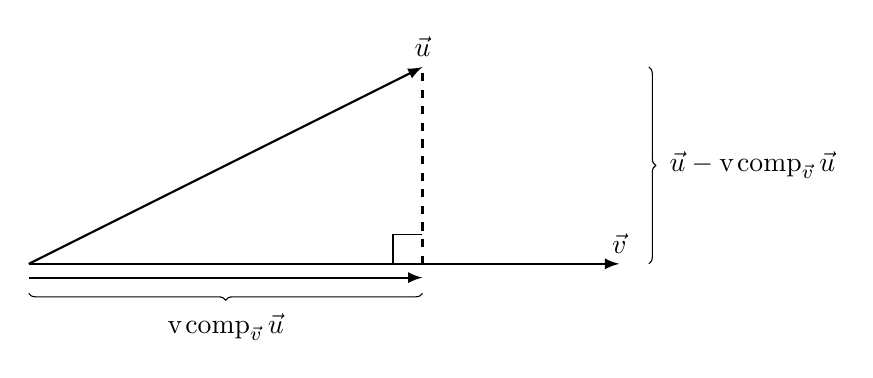
\begin{tikzpicture}[>=latex, scale=2.5]
			\draw[->,thick,black] (0,0) -- (2,1) node [above]
				{$\vec u$};

			\draw[->,thick,black] (0,0) -- (3,0) node [above]
				{$\vec v$};

			\draw[->,thick,black,yshift=-.07cm] (0,0) -- (2,0);
			\draw[decoration={brace, mirror}, decorate, yshift=-.15cm]
				(0,0) -- (2,0) node [midway,below,yshift=-4pt] {$\Comp_{\vec
				v}\vec u$};

			\draw[dashed,thick,black] (2,0) -- (2,1);
			\draw[decoration={brace, mirror}, decorate, xshift=1.15cm]
				(2,0) -- (2,1) node [midway,right,xshift=4pt]
				{$\vec u-\Comp_{\vec v}\vec u$};

			\draw[thin,black] (1.85,0)--(1.85,.15)--(2,.15);
		\end{tikzpicture}
	\end{center}
\end{SaveDefinition}

\begin{SaveDefinition}[key=Subspace, title={Subspace}]
	A non-empty subset $V\subseteq \R^{n}$ is called a \emph{subspace}\index{Subspace}\index[definitions]{Subspaces} if for all $\vec u,\vec v\in V$ and all
	scalars $k$ we have
	\begin{enumerate}
		\item[(i)] $\vec u+\vec v\in V$; and

		\item[(ii)] $k\vec u\in V$.
	\end{enumerate}
\end{SaveDefinition}

\begin{SaveDefinition}[key=TrivialSubspace, title={Trivial Subspace}]
	The subset $\Set{\vec 0}\subseteq\R^n$ is called the \emph{trivial subspace}\index{Subspace!trivial subspace}\index[definitions]{Subspace!trivial subspace}.
\end{SaveDefinition}

\begin{SaveDefinition}[key=Basis, title={Basis}]
	A
	\emph{basis}\index[definitions]{Basis}\index{Basis} for a subspace $\mathcal V$ is a linearly independent set of vectors,
	$\mathcal B$, so that $\Span\mathcal B=\mathcal V$.
\end{SaveDefinition}

\begin{SaveDefinition}[key=Dimension, title={Dimension}]
	The
	\emph{dimension}\index[definitions]{Subspace!dimension}\index{Subspace!dimension} of a subspace $V$ is the number of elements in a basis
	for $V$.
\end{SaveDefinition}

\begin{SaveDefinition}[key=StandardBasisforRn, title={Standard Basis}]
	The \emph{standard basis}\index[definitions]{Basis!standard basis}\index{Basis!standard basis} for $\R^n$ is the set $\Set{\vec e_1,\ldots,\vec e_n}$ where
	\[
		\vec e_1=\matc{1\\0\\0\\\vdots}\qquad
		\vec e_2=\matc{0\\1\\0\\\vdots}\qquad
		\vec e_3=\matc{0\\0\\1\\\vdots}\qquad\cdots.
	\]
	That is $\vec e_i$ is the vector with a $1$ in its
	$i$th coordinate and zeros elsewhere.
\end{SaveDefinition}

\begin{SaveDefinition}[
	key=RepresentationinaBasis,
	title={Representation in a Basis}]

	Let $\mathcal B=\Set{\vec b_1,\ldots,\vec b_n}$ be a basis for a
	subspace $V$ and let $\vec v\in V$. The
	\emph{representation of $\vec v$ in the $\mathcal B$ basis}\index{Vector!representation in a basis}\index[definitions]{Vector!representation in a basis}, notated $[\vec
	v]_{\mathcal B}$\index[symbols]{$[\vec v]_{\mathcal B}$}, is the column matrix
	\[
		[\vec v]_{\mathcal B}= \matc{\alpha_1\\\vdots\\\alpha_n}
	\]
	 where $\alpha_{1},\ldots,\alpha_{n}$ uniquely satisfy
	$\vec v=\alpha_{1}\vec b_{1}+\cdots+\alpha_{n}\vec b_{n}.$

	Conversely,
	\[
		\matc{\alpha_1\\\vdots\\\alpha_n}_{\mathcal B}= \alpha_{1}\vec b_{1}+\cdots
		+\alpha_{n}\vec b_{n}
	\]
	 is notation for the linear combination of $\vec b_{1},\ldots,\vec b_{n}$
	with coefficients $\alpha_{1},\ldots,\alpha_{n}$.
\end{SaveDefinition}

\begin{SaveDefinition}[key=OrthonormalBasis, title={Orthonormal Basis}]
	A basis $\mathcal B=\{\vec b_{1},\ldots,\vec b_{n}\}$ is called
	\emph{orthonormal}\index[definitions]{Basis!orthonormal basis}\index{Basis!orthonormal basis} if every basis vector is a unit vector and all
	basis vectors are orthogonal to each other. That is,
	\[
		\vec b_i\cdot \vec b_j=\begin{cases}
			1 &\text{ if }\quad i=j\\
			0 &\text{ if }\quad i\neq j
		\end{cases}.
	\]
\end{SaveDefinition}

\begin{SaveDefinition}[key=OrientationofaBasis, title={Orientation of a Basis}]
	The ordered basis $\mathcal B=\{\vec b_{1},\ldots,\vec b_{n}\}$ is
	\emph{right-handed}\index[definitions]{Basis!right-handed}\index{Basis!right-handed} or
	\emph{positively oriented}\index[definitions]{Basis!positively oriented}\index{Basis!positively oriented} if it can be continuously transformed to the
	standard basis (with $\vec b_{i}\mapsto \vec e_{i}$) while remaining
	linearly independent throughout the transformation. Otherwise,
	$\mathcal B$ is called
	\emph{left-handed}\index[definitions]{Basis!left-handed}\index{Basis!left-handed} or
	\emph{negatively oriented}\index[definitions]{Basis!negatively oriented}\index{Basis!negatively oriented}.
\end{SaveDefinition}

\begin{SaveDefinition}[key=LinearTransformation, title={Linear Transformation}]
	Let $V$ and $W$ be subspaces. A function $T:V\to W$ is called a
	\emph{linear transformation}\index[definitions]{Linear transformation}\index{Linear transformation} if
	\[
		T(\vec u+\vec v)=T(\vec u)+T(\vec v) \qquad\text{and}\qquad T(\alpha
		\vec v)=\alpha T(\vec v)
	\]
	 for all vectors $\vec u,\vec v\in V$ and all scalars $\alpha$.
\end{SaveDefinition}

\begin{SaveDefinition}[key=ImageofaSet, title={Image of a Set}]
	Let $L:\R^n\to \R^m$ be a transformation and let $X\subseteq \R^n$ be a set. The
	\emph{image of the set $X$ under $L$}\index[definitions]{Set!image of}\index{Set!image of}, denoted $L(X)$\index[symbols]{$L(X)$ (Image of a set)}, is the set
	\[
		L(X)=\Set{\vec y\in \R^m \given \vec y=L(\vec x)\text{ for some }\vec
		x\in X}.
	\]
\end{SaveDefinition}

\begin{SaveDefinition}[key=CompositionofFunctions, title={Composition of Functions}]
	Let $f:A\to B$ and $g:B\to C$. The \emph{composition}\index[definitions]{Function!composition}\index{Function!composition} of $g$ and $f$, notated $g\circ f$\index[symbols]{$g\circ f$},
	is the function $h:A\to C$ defined by
	\[
		h(x)=g\circ f(x) = g\Big(f(x)\Big).
	\]
\end{SaveDefinition}

\begin{SaveDefinition}[key=Range, title={Range}]
	The
	\emph{range} (or
	\emph{image})\index[definitions]{Linear transformation!range (image)}\index{Linear transformation!range (image)} of a linear transformation $T:V\to W$ is the set of vectors
	that $T$ can output. That is,
	\[
		\Range(T)=\Set{\vec y\in W \given \vec y=T\vec x\text{ for some }\vec
		x\in V}.
	\]

\end{SaveDefinition}

\begin{SaveDefinition}[key=NullSpace, title={Null Space}]
	The
	\emph{null space} (or
	\emph{kernel})\index[definitions]{Linear transformation!null space (kernel)}\index{Linear transformations!null space (kernel)} of a linear transformation $T:V\to W$ is the set of vectors
	that get mapped to the zero vector under $T$. That is,
	\[
		\Null(T)=\Set{\vec x\in V \given T\vec x=\vec 0}.
	\]

\end{SaveDefinition}

\begin{SaveDefinition}[
	key=InducedTransformation,
	title={Induced Transformation}]

	Let $M$ be an $n\times m$ matrix. We say $M$
	\emph{induces}\index[definitions]{Matrix!linear transformation induced by}\index{Matrix!linear transformation induced by}\index[definitions]{Linear transformation!induced}\index{Linear transformation!induced} a linear transformation $\mathcal T_{M}:\R^{m}\to\R^{n}$ defined
	by
	\[
		[\mathcal T_{M}\vec v]_{\mathcal E'}= M[\vec v]_{\mathcal E},
	\]
	 where $\mathcal E$ is the standard basis for $\R^{m}$ and $\mathcal E'$
	is the standard basis for $\R^{n}$.
\end{SaveDefinition}

\begin{SaveDefinition}[
	key=Transpose,
	title={Transpose}]

	Let $M$ be an $n\times m$ matrix defined by
	\[
		M=\matc{
			a_{11}&a_{12}&a_{13}&\cdots & a_{1m}\\
		a_{21}&a_{22}&a_{23}&\cdots&a_{2m}\\
		\vdots &\vdots&\vdots &\ddots&\vdots\\
		a_{n1}&a_{n2}&a_{n3}&\cdots&a_{nm}}.
	\]
	The \emph{transpose}\index[definitions]{Matrix!transpose of}\index{Matrix!transpose of} of $M$, notated $M^T$\index[symbols]{$M^T$}, is the $m\times n$ matrix produced by swapping the rows
	and columns of $M$. That is
	\[
		M^T=\matc{
		a_{11}&a_{21}&\cdots&a_{n1}\\
		a_{12}&a_{22}&\cdots&a_{n2}\\
		a_{13}&a_{23}&\cdots&a_{n3}\\
		\vdots&\vdots&\ddots&\vdots\\
		a_{1m}&a_{2m}&\cdots&a_{nm}}.
	\]
\end{SaveDefinition}

\begin{SaveDefinition}[
	key=ElementaryMatrix,
	title={Elementary Matrix}]

	A matrix is called an \emph{elementary matrix}\index[definitions]{Matrix!elementary matrix}\index{Matrix!elementary matrix} if it is an identity matrix with a single elementary row operation applied.
\end{SaveDefinition}

\begin{SaveDefinition}[
	key=MatrixInverse,
	title={Matrix Inverse}]
		
	The \emph{inverse}\index[definitions]{Matrix!inverse of}\index{Matrix!inverse of} of a matrix $A$ is a
		matrix $B$ such that $AB=I$ and $BA=I$.
		In this case, $B$ is called the inverse of $A$ and is notated $A^{-1}$.
\end{SaveDefinition}

\begin{SaveDefinition}[
	key=IdentityFunction,
	title={Identity Function}]
	
	Let $X$ be a set. The \emph{identity function}\index[definitions]{Function!identity function}\index{Function!identity function} with domain and codomain $X$,
	notated $\Ident:X\to X$\index[symbols]{$\Ident$}, is the function satisfying
	\[
		\Ident(x)=x
	\]
	for all $x\in X$.
\end{SaveDefinition}

\begin{SaveDefinition}[
	key=InverseFunction,
	title={Inverse Function}]
		
	Let $f:X\to Y$ be a function. We say $f$ is \emph{invertible}\index[definitions]{Function!invertible function}\index{Function!invertible function} if
	there exists a function $g:Y\to X$ so that $f\circ g=\Ident$ and $g\circ f=\Ident$.
	In this case, we call $g$ an \emph{inverse}\index[definitions]{Function!inverse of}\index{Function!inverse of} of $f$ and write
	\[
		f^{-1}=g.
	\]
\end{SaveDefinition}

\begin{SaveDefinition}[
	key=Onetoone,
	title={One-to-one}]
		
	Let $f:X\to Y$ be a function. We say $f$ is \emph{one-to-one}\index[definitions]{One-to-one function}\index{One-to-one function} (or \emph{injective}\index{Injective function}\index[definitions]{Injective function}) if
	distinct inputs to $f$ produce distinct outputs. That is $f(x)=f(y)$ implies $x=y$.
\end{SaveDefinition}

\begin{SaveDefinition}[
	key=Onto,
	title={Onto}]
		
	Let $f:X\to Y$ be a function.
	We say $f$ is \emph{onto}\index{Onto function}\index[definitions]{Onto function} (or \emph{surjective}\index{Surjective function}\index[definitions]{Surjective function}) if every point in the codomain of $f$ gets mapped to.
	That is $\Range(f)=Y$.
\end{SaveDefinition}

\begin{SaveDefinition}[
	key=IdentityMatrix,
	title={Identity Matrix}]
	
	An \emph{identity matrix}\index{Matrix!identity matrix}\index[definitions]{Matrix!identity matrix} is a square matrix with ones on the diagonal
	and zeros everywhere else. The $n\times n$ identity matrix is denoted $I_{n\times n}$,
	or just $I$ when its size is implied.
\end{SaveDefinition}

\begin{SaveDefinition}[key=FundamentalSubspaces, title={Fundamental Subspaces}]
	\index{Matrix!fundmamental subspaces of}\index[definitions]{Matrix!fundamental subspaces of}
	Associated with any matrix $M$ are three fundamental subspaces: the
	\emph{row space}\index{Matrix!row space}\index[definitions]{Matrix!row space} of $M$, denoted $\Row(M)$\index[symbols]{$\Row(M)$}, is the span of the rows of
	$M$; the
	\emph{column space}\index{Matrix!column space}\index[definitions]{Matrix!column space} of $M$, denoted $\Col(M)$\index[symbols]{$\Col(M)$}, is the span of the
	columns of $M$; and the
	\emph{null space}\index{Matrix!null space}\index[definitions]{Matrix!null space} of $M$, denoted $\Null(M)$\index[symbols]{$\Null(M)$}, is the set of solutions to
	$M\vec x=\vec 0$.
\end{SaveDefinition}

\begin{SaveDefinition}[key=RankofaLinearTransformation, title={Rank of a Linear Transformation}]
	For a linear transformation $T:\R^n\to \R^m$, the
	\emph{rank}\index[definitions]{Linear transformation!rank}\index{Linear transformation!rank} of $T$, denoted $\Rank(T)$\index[symbols]{$\Rank(T)$}, is the dimension of the range of
	$T$.
\end{SaveDefinition}

\begin{SaveDefinition}[key=RankofaMatrix, title={Rank of a Matrix}]
	Let $M$ be a matrix.
	The \emph{rank}\index[definitions]{Matrix!rank}\index{Matrix!rank} of $M$, denoted $\Rank(M)$\index[symbols]{$\Rank(M)$}, is the rank of
	the linear transformation induced by $M$.
\end{SaveDefinition}

\begin{SaveDefinition}[key=NullityofaMatrix, title={Nullity of a Matrix}]
	Let $M$ be a matrix.
	The \emph{nullity}\index[definitions]{Matrix!nullity}\index{Matrix!nullity} of $M$, denoted $\Nullity(M)$\index[symbols]{$\Nullity(M)$}, is the nullity of
	the linear transformation induced by $M$.
\end{SaveDefinition}

\begin{SaveDefinition}[key=Rank, title={Rank}]
	For a linear transformation $T:\R^n\to \R^m$, the
	\emph{rank} of $T$, denoted $\Rank(T)$, is the dimension of the range of
	$T$.\index[definitions]{Linear transformation!rank}\index{Linear transformation!rank}

	For an $m\times n$ matrix $M$, the
	\emph{rank} of $M$, denoted $\Rank(M)$, is the dimension of the 
	column space of $M$.\index[definitions]{Matrix!nullity}\index{Matrix!nullity}
\end{SaveDefinition}

\begin{SaveDefinition}[key=Nullity, title={Nullity}]
	For a linear transformation $T:\R^n\to \R^m$, the
	\emph{nullity} of $T$, denoted $\Nullity(T)$, is the dimension of the null space of
	$T$.\index[definitions]{Linear transformation!nullity}\index{Linear transformation!nullity}
\end{SaveDefinition}

\begin{SaveDefinition}[key=ChangeofBasisMatrix, title={Change of Basis Matrix}]
	Let $\mathcal A$ and $\mathcal B$ be bases for $\R^n$. The matrix $M$ is called
	a \emph{change of basis} matrix\index[definition]{Change of basis matrix}\index{Change of basis matrix} (which converts from $\mathcal A$ to $\mathcal B$) if
	for all $\vec x\in \R^n$
	\[
		M[\vec x]_{\mathcal A}=[\vec x]_{\mathcal B}.
	\]
	 Notationally, $\BasisChange{\mathcal A}{\mathcal B}$\index[symbols]{$\BasisChange{\mathcal A}{\mathcal B}$}
	stands for the change of basis matrix converting from $\mathcal A$ to $\mathcal B$,
	and we may write $M=\BasisChange{\mathcal A}{\mathcal B}$.
\end{SaveDefinition}

\begin{SaveDefinition}[key=LinearTransformationinaBasis, title={Linear Transformation in a Basis}]
	Let $\mathcal T:\R^n\to\R^n$ be a linear transformation and let $\mathcal B$ be a
	basis for $\R^n$. The \emph{matrix for $\mathcal T$ with respect to $\mathcal B$}, notated
	$[\mathcal T]_{\mathcal B}$,
	is the $n\times n$ matrix satisfying
	\[
		[\mathcal T\vec x]_{\mathcal B} = [\mathcal T]_{\mathcal B}[\vec x]_{\mathcal B}.
	\]
	In this case, we say the matrix $[\mathcal T]_{\mathcal B}$\index[symbols]{$[\mathcal T]_{\mathcal B}$} is the representation
	of $\mathcal T$ in the $\mathcal B$ basis.
	\index{Matrix!of a linear transformation}\index[definitions]{Matrix!of a linear transformation}\index{Linear transformation!representation in a basis}\index[definitions]{Linear transformation!representation in a basis}
\end{SaveDefinition}

\begin{SaveDefinition}[key=SimilarMatrices, title={Similar Matrices}]
	The matrices $A$ and $B$ are called
	\emph{similar matrices}\index[definitions]{Matrix!similar matrices},
	denoted $A\sim B$\index[symbols]{$\sim$}, if $A$ and $B$ represent the
	same linear transformation but in possibly different bases. Equivalently,
	$A\sim B$ if there is an invertible matrix $X$ so that
	\[
		A=XBX^{-1}.
	\]

\end{SaveDefinition}

\begin{SaveDefinition}[key=Unitncube, title={Unit $n$-cube}]
	The
	\emph{unit $n$-cube}\index[definitions]{Unit $n$-cube ($C_n$)}\index{Unit $n$-cube ($C_n$)} is the $n$-dimensional cube with sides given by the
	standard basis vectors and lower-left corner located at the origin. That
	is
	\[
		C_{n}=\Set*{\vec x\in\R^n:\vec x=\sum_{i=1}^n\alpha_i\vec e_i\text{
		for some }\alpha_1,\ldots,\alpha_n\in[0,1]}=[0,1]^{n}.
	\]\index[symbols]{$C_n$}

\end{SaveDefinition}

\begin{SaveDefinition}[key=Determinant, title={Determinant}]
	The
	\emph{determinant}\index{Determinant}\index[definitions]{Determinant} of a linear transformation $\mathcal T:\R^{n}\to \R^{n}$, denoted $\det(\mathcal T)$\index[symbols]{$\det(\mathcal T)$} or $\Abs{\mathcal T}$\index[symbols]{$\Abs{\mathcal T}$}, is
	the oriented volume of the image of the unit $n$-cube. The determinant of
	a square matrix is the determinant of its induced transformation.
\end{SaveDefinition}

\begin{SaveDefinition}[key=OrientationPreservingLinearTransformation, title={Orientation Preserving Linear Transformation}]
	Let $\mathcal T:\R^n\to\R^n$ be a linear transformation. We say $\mathcal T$
	is \emph{orientation preserving}\index[definitions]{Linear transformation!orientation preserving}\index{Linear transformation!orientation preserving} if the ordered basis $\Set{\mathcal T(\vec e_1),\ldots, \mathcal T(\vec e_n)}$
	is positively oriented  and we say $\mathcal T$
	is \emph{orientation reversing}\index[definitions]{Linear transformation!orientation reversing}\index{Linear transformation!orientation reversing} if the ordered basis $\Set{\mathcal T(\vec e_1),\ldots, \mathcal T(\vec e_n)}$
	is negatively oriented. If $\Set{\mathcal T(\vec e_1),\ldots, \mathcal T(\vec e_n)}$
	is not a basis for $\R^n$, then $\mathcal T$ is neither orientation preserving nor orientation reversing.
\end{SaveDefinition}

\begin{SaveDefinition}[key=Eigenvector, title={Eigenvector}]
	Let $X$ be a linear transformation or a matrix. An
	\emph{eigenvector}\index[definitions]{Eigenvector}\index{Eigenvector} for $X$ is a non-zero vector that doesn't change
	directions when $X$ is applied. That is, $\vec v\neq \vec 0$ is an
	eigenvector for $X$ if
	\[
		X\vec v=\lambda \vec v
	\]
	 for some scalar $\lambda$. We call $\lambda$ the
	\emph{eigenvalue}\index[definitions]{Eigenvalue}\index{Eigenvalue} of $X$ corresponding to the eigenvector $\vec v$.
\end{SaveDefinition}

\begin{SaveDefinition}[
	key=CharacteristicPolynomial,
	title={Characteristic Polynomial}]

	For a matrix $A$, the
	\emph{characteristic polynomial}\index{Characteristic polynomial}\index[definition]{Characteristic Polynomial} of $A$ is
	\[
		\chr(A)=\det(A-\lambda I).
	\]\index[symbols]{$\chr(A)$}

\end{SaveDefinition}

\begin{SaveDefinition}[key=Diagonalizable, title={Diagonalizable}]
	A matrix is
	\emph{diagonalizable}\index{Matrix!diagonalizable}\index[definitions]{Matrix!diagonalizible} if it is similar to a diagonal matrix.
\end{SaveDefinition}

\begin{SaveDefinition}[key=Eigenspace, title={Eigenspace}]
	Let $A$ be an $n\times n$ matrix with eigenvalues
	$\lambda_{1},\ldots,\lambda_{m}$. The
	\emph{eigenspace}\index[definitions]{Eigenspace}\index{Eigenspace} of $A$ corresponding to the eigenvalue $\lambda_{i}$
	is the null space of $A-\lambda_{i} I$. That is, it is the space spanned
	by all eigenvectors that have the eigenvalue $\lambda_{i}$.

	The
	\emph{geometric multiplicity}\index[definitions]{Eigenvalue!geometric multiplicity}\index{Eigenvalue!geometric multiplicity} of an eigenvalue $\lambda_{i}$ is the
	dimension of the corresponding eigenspace. The
	\emph{algebraic multiplicity}\index[definitions]{Eigenvalue!algebraic multiplicity}\index{Eigenvalue!algebraic multiplicity} of $\lambda_{i}$ is the number of times
	$\lambda_{i}$ occurs as a root of the characteristic polynomial of $A$ (i.e.,
	the number of times $x-\lambda_{i}$ occurs as a factor).
\end{SaveDefinition}




%%
%% End Definitions
%%






\pagestyle{empty}

\begin{tikzpicture}[remember picture,overlay, shift={(current page.north west)}, >=latex]
	\definecolor{coverblue}{HTML}{ffd33c}
	\definecolor{coverpink}{HTML}{ff97e8}
	\definecolor{coveraccentpink}{HTML}{ffd33c}
	\definecolor{coverorange}{HTML}{ffffff}
	\definecolor{covershade}{HTML}{3f004d}


	\newcommand{\LINEARALGEBRAoutline}{(26.3109,27.9294) -- (26.3109,25.4774) --
      (20.8620,25.4774) -- (20.8620,9.8119) -- (18.5190,9.8119) -- (18.5190,27.9294)
      -- cycle

	  (30.0421,12.3456) .. controls (30.7232,12.3456)
      and (31.2953,11.8008) .. (31.2953,11.0924) .. controls (31.2953,10.4113) and
      (30.7232,9.8392) .. (30.0421,9.8392) .. controls (29.3337,9.8392) and
      (28.7888,10.4113) .. (28.7888,11.0924) .. controls (28.7888,11.8008) and
      (29.3337,12.3456) .. (30.0421,12.3456) -- cycle(31.2136,27.9294) --
      (31.2136,14.3072) -- (28.9250,14.3072) -- (28.9250,27.9294) -- cycle
     
	  (44.8196,27.9294) -- (44.8196,19.7561) ..
      controls (44.8196,18.2577) and (44.2202,16.8954) .. (43.2394,15.9146) ..
      controls (42.2586,14.9338) and (40.8964,14.3072) .. (39.3979,14.3072) ..
      controls (38.3082,14.3072) and (37.0549,14.9066) .. (36.3738,15.7512) --
      (36.3738,14.6342) -- (34.0036,14.6342) -- (34.0036,27.9294) --
      (36.3738,27.9294) -- (36.3738,19.7561) .. controls (36.3738,18.9660) and
      (36.7280,18.2032) .. (37.2729,17.6583) .. controls (37.8178,17.1134) and
      (38.5534,16.7592) .. (39.3979,16.7592) .. controls (40.2425,16.7592) and
      (40.9781,17.0861) .. (41.5230,17.6310) .. controls (42.0679,18.1759) and
      (42.4221,18.9115) .. (42.4221,19.7561) -- (42.4221,27.9294) -- cycle

     (60.6302,22.1536) .. controls (60.9571,19.9468)
      and (60.2488,17.9035) .. (58.6959,16.3233) .. controls (57.4699,15.0701) and
      (55.7262,14.3345) .. (53.8464,14.3345) .. controls (51.9665,14.3345) and
      (50.2229,15.0701) .. (48.9969,16.3233) .. controls (47.7709,17.5765) and
      (46.9808,19.3202) .. (46.9808,21.2000) .. controls (46.9808,23.0799) and
      (47.7709,24.8235) .. (48.9969,26.0495) .. controls (50.2229,27.2755) and
      (51.9665,28.0656) .. (53.8464,28.0656) .. controls (56.3528,28.0656) and
      (58.4779,26.7579) .. (59.8674,24.4966) -- (57.7968,23.2706) .. controls
      (56.7888,24.8235) and (55.4810,25.6136) .. (53.8464,25.6136) .. controls
      (52.8383,25.6136) and (51.9120,25.2867) .. (51.1764,24.7146) .. controls
      (50.4136,24.1424) and (49.5962,23.1071) .. (49.5962,22.1536) --
      cycle(53.8464,16.5685) .. controls (56.1621,16.5685) and (58.0965,18.2577) ..
      (58.0965,20.0558) -- (49.5962,20.0558) .. controls (49.5962,18.2577) and
      (51.5578,16.5685) .. (53.8464,16.5685) -- cycle
     
	(76.3834,27.9294) -- (76.3834,14.6342) --
      (73.9314,14.6342) -- (73.9314,16.4323) .. controls (72.8416,15.1246) and
      (71.2342,14.3617) .. (69.4906,14.3617) .. controls (67.5562,14.3617) and
      (65.8943,15.0973) .. (64.6411,16.3506) .. controls (63.3878,17.6038) and
      (62.6250,19.3474) .. (62.6250,21.2273) .. controls (62.6250,23.1071) and
      (63.3878,24.8508) .. (64.6411,26.0768) .. controls (65.8943,27.3028) and
      (67.5562,28.0656) .. (69.4906,28.0656) .. controls (71.2342,28.0656) and
      (72.8144,27.1665) .. (73.9314,25.8588) -- (73.9314,27.9294) --
      cycle(69.4906,16.7865) .. controls (70.7166,16.7865) and (71.8336,17.2769) ..
      (72.6237,18.0669) .. controls (73.4137,18.8570) and (73.9041,20.0013) ..
      (73.9041,21.2273) .. controls (73.9041,22.4533) and (73.4137,23.5703) ..
      (72.6237,24.3604) .. controls (71.8336,25.1505) and (70.7166,25.6409) ..
      (69.4906,25.6409) .. controls (68.2646,25.6409) and (67.1203,25.1505) ..
      (66.3302,24.3604) .. controls (65.5401,23.5703) and (65.0497,22.4533) ..
      (65.0497,21.2273) .. controls (65.0497,20.0013) and (65.5401,18.8570) ..
      (66.3302,18.0669) .. controls (67.1203,17.2769) and (68.2646,16.7865) ..
      (69.4906,16.7865) -- cycle

     (87.4637,15.5877) .. controls (86.2377,14.5797)
      and (85.2025,14.1983) .. (84.0309,14.1983) .. controls (83.2409,14.1983) and
      (82.5598,14.3617) .. (81.9331,14.6614) .. controls (80.2167,15.5605) and
      (79.1270,17.2769) .. (79.1270,19.2657) -- (79.1270,27.9294) --
      (81.4700,27.9294) -- (81.4700,19.2657) .. controls (81.4700,18.5301) and
      (81.7697,17.8762) .. (82.2328,17.3858) .. controls (82.6960,16.8954) and
      (83.3498,16.6230) .. (84.0309,16.6230) .. controls (84.3851,16.6230) and
      (84.7938,16.7320) .. (85.2025,16.9227) -- cycle

    (118.1877,27.9294) -- (111.8942,9.8392) --
      (109.1698,9.8392) -- (102.8764,27.9294) -- (105.4646,27.9294) --
      (107.6986,21.5542) -- (113.3654,21.5542) -- (115.5995,27.9294) --
      cycle(112.5753,19.2657) -- (108.4614,19.2657) -- (110.5320,13.3537) -- cycle

    (122.6779,27.9294) -- (122.6779,9.8119) --
      (120.4983,9.8119) -- (120.4983,27.9294) -- cycle

    (131.9609,33.7324) .. controls (133.8408,33.7324)
      and (135.5844,32.9423) .. (136.8104,31.6891) .. controls (138.0364,30.4359)
      and (138.8265,28.7195) .. (138.8265,26.7851) -- (138.8265,14.5524) --
      (136.3745,14.5524) -- (136.3745,16.4323) .. controls (135.7207,15.5605) and
      (134.1405,14.3072) .. (131.9337,14.3072) .. controls (130.0538,14.3072) and
      (128.3374,15.0701) .. (127.1114,16.2688) .. controls (125.8855,17.4948) and
      (125.0954,19.2112) .. (125.0954,21.0911) .. controls (125.0954,22.9437) and
      (125.8582,24.7146) .. (127.0842,26.0223) .. controls (128.3102,27.3573) and
      (130.0538,28.2018) .. (131.9337,28.2018) .. controls (133.6773,28.2018) and
      (135.1758,27.4662) .. (136.3745,26.1313) -- (136.3745,26.7851) .. controls
      (136.3745,28.0111) and (135.8841,29.1281) .. (135.0940,29.9455) .. controls
      (134.3039,30.7628) and (133.1869,31.2804) .. (131.9609,31.2804) .. controls
      (130.6260,31.2804) and (129.4817,30.7083) .. (128.5009,29.5640) --
      (126.3486,30.8445) .. controls (127.8743,32.6971) and (129.7814,33.7324) ..
      (131.9609,33.7324) -- cycle(131.9337,16.7865) .. controls (133.1597,16.7865)
      and (134.2767,17.2769) .. (135.0668,18.0942) .. controls (135.8569,18.9115)
      and (136.3473,20.0558) .. (136.3473,21.2818) .. controls (136.3473,22.5078)
      and (135.8569,23.6520) .. (135.0668,24.4421) .. controls (134.2768,25.2322)
      and (133.1597,25.7498) .. (131.9337,25.7498) .. controls (130.7077,25.7498)
      and (129.5907,25.2322) .. (128.8006,24.4421) .. controls (128.0106,23.6520)
      and (127.4929,22.5078) .. (127.4929,21.2818) .. controls (127.4929,20.0558)
      and (128.0106,18.9115) .. (128.8006,18.0942) .. controls (129.5907,17.2769)
      and (130.7077,16.7865) .. (131.9337,16.7865) -- cycle

     (154.9211,22.1536) .. controls (155.2480,19.9468)
      and (154.5397,17.9035) .. (152.9868,16.3233) .. controls (151.7608,15.0701)
      and (150.0171,14.3345) .. (148.1373,14.3345) .. controls (146.2574,14.3345)
      and (144.5138,15.0701) .. (143.2878,16.3233) .. controls (142.0618,17.5765)
      and (141.2717,19.3202) .. (141.2717,21.2000) .. controls (141.2717,23.0799)
      and (142.0618,24.8235) .. (143.2878,26.0495) .. controls (144.5138,27.2755)
      and (146.2574,28.0656) .. (148.1373,28.0656) .. controls (150.6437,28.0656)
      and (152.7688,26.7579) .. (154.1583,24.4966) -- (152.0877,23.2706) .. controls
      (151.0796,24.8235) and (149.7719,25.6136) .. (148.1373,25.6136) .. controls
      (147.1292,25.6136) and (146.2029,25.2867) .. (145.4673,24.7146) .. controls
      (144.7045,24.1424) and (143.8871,23.1071) .. (143.8871,22.1536) --
      cycle(148.1373,16.5685) .. controls (150.4530,16.5685) and (152.3874,18.2577)
      .. (152.3874,20.0558) -- (143.8871,20.0558) .. controls (143.8871,18.2577) and
      (145.8487,16.5685) .. (148.1373,16.5685) -- cycle
    
    (164.3744,28.0656) .. controls (166.2543,28.0656)
      and (168.0252,27.3028) .. (169.2512,26.0223) .. controls (170.4772,24.7418)
      and (171.2673,23.0254) .. (171.2673,21.0911) .. controls (171.2673,19.1567)
      and (170.4772,17.4403) .. (169.2512,16.1598) .. controls (168.0252,14.8794)
      and (166.2543,14.1165) .. (164.3744,14.1165) .. controls (162.0859,14.1165)
      and (160.5330,15.3153) .. (159.8519,16.2688) -- (159.8519,9.8392) --
      (157.4544,9.8392) -- (157.4544,27.9294) -- (159.8519,27.9294) --
      (159.8519,25.8316) .. controls (160.9689,27.1665) and (162.6308,28.0656) ..
      (164.3744,28.0656) -- cycle(164.3744,16.5958) .. controls (165.6004,16.5958)
      and (166.7175,17.0861) .. (167.5075,17.9035) .. controls (168.2976,18.7208)
      and (168.8153,19.8651) .. (168.8153,21.0911) .. controls (168.8153,22.3715)
      and (168.2976,23.4613) .. (167.5075,24.2787) .. controls (166.7175,25.0960)
      and (165.6004,25.6136) .. (164.3744,25.6136) .. controls (163.1484,25.6136)
      and (162.0042,25.0960) .. (161.2141,24.2787) .. controls (160.4240,23.4613)
      and (159.9064,22.3715) .. (159.9064,21.0911) .. controls (159.9064,19.8651)
      and (160.4240,18.7208) .. (161.2141,17.9035) .. controls (162.0042,17.0862)
      and (163.1484,16.5958) .. (164.3744,16.5958) -- cycle

     (182.0739,15.5877) .. controls (180.8479,14.5797)
      and (179.8126,14.1983) .. (178.6411,14.1983) .. controls (177.8510,14.1983)
      and (177.1699,14.3617) .. (176.5433,14.6614) .. controls (174.8269,15.5605)
      and (173.7371,17.2769) .. (173.7371,19.2657) -- (173.7371,27.9294) --
      (176.0801,27.9294) -- (176.0801,19.2657) .. controls (176.0801,18.5301) and
      (176.3798,17.8762) .. (176.8430,17.3858) .. controls (177.3061,16.8954) and
      (177.9600,16.6230) .. (178.6411,16.6230) .. controls (178.9953,16.6230) and
      (179.4039,16.7320) .. (179.8126,16.9227) -- cycle

     (195.3112,27.9294) -- (195.3112,14.6342) --
      (192.8592,14.6342) -- (192.8592,16.4323) .. controls (191.7695,15.1246) and
      (190.1620,14.3617) .. (188.4184,14.3617) .. controls (186.4841,14.3617) and
      (184.8222,15.0973) .. (183.5689,16.3506) .. controls (182.3157,17.6038) and
      (181.5528,19.3474) .. (181.5528,21.2273) .. controls (181.5528,23.1071) and
      (182.3157,24.8508) .. (183.5689,26.0768) .. controls (184.8222,27.3028) and
      (186.4841,28.0656) .. (188.4184,28.0656) .. controls (190.1620,28.0656) and
      (191.7422,27.1665) .. (192.8592,25.8588) -- (192.8592,27.9294) --
      cycle(188.4184,16.7865) .. controls (189.6444,16.7865) and (190.7614,17.2769)
      .. (191.5515,18.0669) .. controls (192.3416,18.8570) and (192.8320,20.0013) ..
      (192.8320,21.2273) .. controls (192.8320,22.4533) and (192.3416,23.5703) ..
      (191.5515,24.3604) .. controls (190.7614,25.1505) and (189.6444,25.6409) ..
      (188.4184,25.6409) .. controls (187.1924,25.6409) and (186.0481,25.1505) ..
      (185.2581,24.3604) .. controls (184.4680,23.5703) and (183.9776,22.4533) ..
      (183.9776,21.2273) .. controls (183.9776,20.0013) and (184.4680,18.8570) ..
      (185.2581,18.0669) .. controls (186.0481,17.2769) and (187.1924,16.7865) ..
      (188.4184,16.7865) -- cycle}

	\begin{scope}
		\node[anchor=south east,inner sep=0pt,outer sep=0pt,] 
		at (current page.south east) {\includegraphics[width=\paperwidth, height=\paperheight]{images/orangeback.jpg}};

		\fill[path fading=north,covershade] (0,2.2in) rectangle ([yshift=-1.01in, xshift=2pt]current page.north east);
		\fill[covershade] (0,-1in) rectangle ([yshift=-2.05in]current page.north east);
		\fill[path fading=south, covershade] (0,-2in) rectangle ([xshift=1in,yshift=2in]current page.south east);
	\end{scope}


  \begin{scope}[yscale=-1, xscale=1, x=2.7pt, y=2.7pt,line join=miter,line cap=butt,line width=1.3pt, yshift=2.3cm, xshift=.7cm,
	  ]

	  \coordinate (E) at (57.55,23.15);
	  \coordinate (A) at (195.3,27.9);
	  \coordinate (C) at (195.3,104);
	  \coordinate (SUB) at (141, 30);
		
	  \fill[coverblue, opacity=.7] \LINEARALGEBRAoutline;
	  \draw[coverblue, line width=1.3pt] \LINEARALGEBRAoutline;
  \end{scope}

  	\coordinate (X) at (3, -15);
	\path (E) --  (C)  
		coordinate[pos=0] (X1)
		coordinate[pos=.017] (X2)
		coordinate[pos=.08] (X3)
		coordinate[pos=.2] (X4)
		coordinate[pos=.5] (X5)
		coordinate[pos=1] (X6)
		-- (A);
	\draw[coverpink, line width=1.3pt] (E) --  (C)  
		-- (A);
	\begin{scope}[coverorange, line width=0.5pt]
		\draw[->] 
			(X) -- (X1) node[pos=.5, above left] {\Large $\vec u$};
		\draw[->] 
			(X) -- (X2);
		\draw[->] 
			(X) -- (X3);
		\draw[->] 
			(X) -- (X4);
		\draw[->, coveraccentpink, line width=1.3pt] 
			(X) -- (X5) node[pos=.6, below right] {\Large $\vec w_{\alpha}=\alpha {\color{coverorange}\vec u} + (1-\alpha){\color{coverorange}\vec v}$};
		\draw[->] 
			(X) -- (X6) node[pos=.7, below right] {\Large $\vec v$};
	\end{scope}

	\path[white] (SUB) node[anchor=north west] {\Large \bfseries \sffamily \coversubtitle};

\newcommand{\authornames}{\huge \sffamily \bfseries \begin{tabular}{r}Jason Siefken\end{tabular}}
	\newcommand{\ypadd}{.5em}
	\newcommand{\xpadd}{1em}

	\draw (0, -24) node[right, xshift=10em] (AUTHOR) {\phantom{\authornames}};
	\path let \p1 = (AUTHOR.north) in coordinate (Ab1) at (0,\y1+\ypadd);
	\path let \p1 = (AUTHOR.north east) in coordinate (Ab2) at (\x1+\xpadd,\y1+\ypadd);
	\path let \p1 = (AUTHOR.south east) in coordinate (Ab3) at (\x1+\xpadd,\y1-\ypadd);
	\path let \p1 = (AUTHOR.south) in coordinate (Ab4) at (0,\y1-\ypadd);

	\path[fill=covershade, path fading=west, opacity=.8] (Ab1) -- (Ab2) -- (Ab3) -- (Ab4);
	\draw[covershade!80!black, line width=1.3pt] (Ab1) -- (Ab2) -- (Ab3) -- (Ab4);
	\draw (0, -24) node[right, xshift=10em, white] (AUTHOR) {\authornames};

\end{tikzpicture}


\newpage

\begin{bookonly}
	\clearpage
	\hbox{}
	\newpage
	\begin{center}
	{\color{myorange}\huge\bfseries\sffamily Linear Algebra}\\

\vspace{.2in}
{
\it \copyright\,Jason Siefken, 2016--2022 \\
Creative Commons By-Attribution Share-Alike\, \makebox(30,5){\includegraphics[height=1.2em]{by-sa.pdf}}
}
\end{center}

\section*{About this Book}

\subsection*{For the student}

This book is your introductory guide to linear algebra. It is divided into
\emph{modules}, and each module is further divided into \emph{exposition},
\emph{practice problems}, and \emph{core exercises}.

The \emph{exposition} is easy to find---it's the text that starts each
module and explains the big ideas of linear algebra.  The \emph{practice
problems} immediately follow the exposition and are there so you can
practice with concepts you've learned.  Following the practice problems
are the \emph{core exercises}. The core exercises build up, through
examples, the concepts discussed in the exposition.

To optimally learn from this text, you should:
\begin{itemize}
	\item Start each module by reading through the \emph{exposition} to get familiar with the main ideas and 
		linear algebra terminology.

	\item Work through the \emph{core exercises} to develop an understanding and intuition behind the main ideas
		and their subtleties.

	\item Re-read the \emph{exposition} and identify which concepts each core exercise connects with.

	\item Work through the \emph{practice problems}. These will serve as a check on whether you've understood
		the main ideas well enough to apply them.
\end{itemize}

{\bf The core exercises.} Most (but not all) core exercises will be
worked through during lecture time, and there is space for you to work
provided after each
of the core exercises. The point of the core exercises is to develop the main ideas of
linear algebra by exploring examples. When working on core exercises, think
``it's the journey that matters not the destination''. The
answers are not the point! If you're struggling, keep with it. The
concepts you struggle with you remember well, and if you look up the
answer, you're likely to forget just a few minutes later. 

{\bf So many definitions.} A big part of linear algebra is learning precise and
technical language\footnote{ Beyond three dimensions, things get very confusing
very quickly.  Having precise definitions allows us to make arguments that
rely on logic instead of intuition; and logic works in all dimensions.}.
There are many terms and definitions you need to learn, and by far the
best way to successfully learn these terms is to understand where they
come from, why they're needed, and practice using them. That is, don't
try to memorize definitions word for word. Instead memorize the idea
and \emph{reconstruct} the definition; go through the core exercises and
identify which definitions appear where; and explain linear algebra to
others using these technical terms.

{\bf Contributing to the book.} Did you find an error? Do you
have a better way to explain a linear algebra concept? Please,
contribute to this book!  This book is open-source, and we welcome
contributions and improvements. To contribute to/fix part of
this book, make a \emph{Pull Request} or open an \emph{Issue} at
\url{https://github.com/siefkenj/IBLLinearAlgebra}. If you contribute,
you'll get your name added to the contributor list.


\subsection*{For the instructor}

This book is designed for a one-semester introductory linear algebra course
course with a focus on geometry (MAT223 at the University of Toronto). 
It has not been designed for an ``intro to proofs''-style course, but could be adapted for one.

Unlike a traditional textbook that is grouped into chapters and sections
by subject, this book is grouped into modules. Each module contains exposition
about a subject, practice problems (for students to work on by themselves), and core exercises
(for students to work on with your guidance). Modules group related concepts, but the 
modules have been designed to facilitate learning linear algebra rather than to serve
as a reference. For example, information about change-of-basis is spread across several non-consecutive
modules; each time change-of-basis is readdressed, more detail is added.

{\bf Using the book.} This book has been designed for use in large 
active-learning classrooms driven by a \emph{think, pair-share}/small-group-discussion format.
Specifically, the \emph{core exercises} (these are the problems which aren't labeled ``Practice Problems''
and for which space is provided to write answers) are designed for use during class time.

A typical class day looks like:
\begin{enumerate}
	\item {\bf Student pre-reading.} Before class, students will read through the relevant module.

	\item {\bf Introduction by instructor.} This may involve giving a definition,
		a broader context for the day's topics, or answering questions.

	\item {\bf Students work on problems.} Students work individually or in pairs/small groups
		on the prescribed core exercise. During this time the instructor moves
		around the room addressing questions that students may have and giving
		one-on-one coaching.

	\item {\bf Instructor intervention.} When most students have successfully solved
		the problem, the instructor refocuses the class by providing an
		explanation or soliciting explanations from students.
		This is also time for the instructor to ensure that everyone has
		understood the main point of the exercise (since it is sometimes
		easy to miss the point!).

		If students are having trouble, the instructor can give hints
		and additional guidance to ensure students' struggle is productive.

	\item {\bf Repeat step 3.}
\end{enumerate}

Using this format, students are thinking (and happily so) most of the class. Further,
after struggling with a question, students are especially primed to hear the insights of the instructor.

{\bf Conceptual lean.}
The \emph{core exercises} are geared towards concepts instead of computation, though some core exercises
focus on simple computation. They also have a geometric lean. Vectors are initially
introduced with familiar coordinate notation, but eventually, coordinates are understood to be
\emph{representations} of vectors rather than ``true'' geometric vectors, and objects like the
determinant are defined via oriented volumes rather than formulas involving matrix entries.

Specifically lacking are exercises focusing on the mechanical skills of row reduction and
computing matrix inverses. Students must practice these skills, but they require little instructor
intervention and so can be learned outside of lecture (which is why core exercises don't focus on
these skills).

{\bf How to prepare.}
Running an active-learning classroom is less scripted than lecturing.
The largest
challenges are: (i) understanding where students are at, (ii) figuring out what to do given the current
understanding of the students, and (iii) timing.

To prepare for a class day, you should:
\begin{enumerate}
	\item {\bf Strategize about learning objectives.} Figure out what the point of the day's lesson is
		and brain storm some examples that would illustrate that point.
	\item {\bf Work through the core exercises.} 
	%	By working through the exercises yourself, you
	%	will be ready to build off student reasoning, and better able to direct a class towards
	%	the important ideas\footnote{ The content of linear algebra is fairly non-linear. One of the hardest parts
	%	of teaching linear algebra is coming up with an explanation that only depends on ideas that have already been taught.}.
	\item {\bf Reflect.} Reflect on how each core exercise addresses the day's goals. Compare with the examples you
		brainstormed and prepare follow-up questions that you can use in class to test for understanding.
	\item {\bf Schedule.} Write timestamps next to each core exercise indicating at what minute you hope
		to start each exercise. Give more time for the exercises that you judge as foundational, and be prepared
		to triage. It's appropriate to leave exercises or parts of exercises for homework, but change the order
		of exercises at your peril---they really do build on each other.
\end{enumerate}

A typical
50 minute class is enough to get through 2--3 core exercises (depending on the difficulty), and class observations
show that class time is split 50/50 between students working and instructor explanations.

\subsection*{License}
 Unless otherwise mentioned, pages of this document are licensed under
the Creative Commons By-Attribution Share-Alike License. That means, you are free
to use, copy, and modify this document provided that you provide attribution to the
previous copyright holders and you release your derivative work under the same license.
Full text of the license is at \url{http://creativecommons.org/licenses/by-sa/4.0/}

If you modify this document, you may add your name to the copyright list. Also,
if you think your contributions would be helpful to others, consider making a
pull request, or opening an \emph{issue} at \url{https://github.com/siefkenj/IBLLinearAlgebra}

{\bf Incorporated content.}
Content from other sources is reproduced here with permission and retains the
Author's copyright. Please see the footnote of each page to verify the
copyright.

Included in this text are tasks created by the Inquiry-Oriented Linear Algebra (IOLA) project. Details
about these tasks can be found on their website \url{http://iola.math.vt.edu/}. Also included are some
practice problems from Beezer's \emph{A First Course in Linear Algebra} (marked with the symbol \beezer next to the
problem), and from Hefferon's \emph{Linear Algebra} (marked with the symbol \hefferon next to the problem).

{\bf Contributing.} You can report errors in the book or contribute to the book by filing an \emph{Issue} or
a \emph{Pull Request} on the book's GitHub page: \url{https://github.com/siefkenj/IBLLinearAlgebra/}


	\section*{Contributors}
	% sorting code from
% http://tex.stackexchange.com/questions/121489/alphabetically-display-the-items-in-itemize
\newcommand{\sortitem}[2][\relax]{%
  \DTLnewrow{list}% Create a new entry
  \ifx#1\relax
    \DTLnewdbentry{list}{sortlabel}{#2}% Add entry sortlabel (no optional argument)
  \else
    \DTLnewdbentry{list}{sortlabel}{#1}% Add entry sortlabel (optional argument)
  \fi%
  \DTLnewdbentry{list}{description}{#2}% Add entry description
}
\newenvironment{sortedlist}{%
  \DTLifdbexists{list}{\DTLcleardb{list}}{\DTLnewdb{list}}% Create new/discard old list
}{%
  \DTLsort{sortlabel}{list}% Sort list
  \begin{itemize*}[label={\color{mypink}$\circ$}]%
    \DTLforeach*{list}{\theDesc=description}{%
      \item \theDesc}% Print each item
  \end{itemize*}%
}

This book is a collaborative effort.  The following people have contributed
to its creation:
\begin{quote}
\begin{sortedlist}
	\sortitem[Wang]{Tianhao (Patrick) Wang}
	\sortitem[Khan]{Sameul Khan}
	\sortitem[King]{Avery King}
	\sortitem[Frohlich]{Jesse Frohlich}
	\sortitem[Wolske]{Zack Wolske}
	\sortitem[Le]{Dan Le}
	\sortitem[Qiu]{Ruo Ning (Nancy) Qiu}
    \sortitem[Li]{Xintong (Alucart) Li}
    \sortitem[Chen]{Shukui Chen}
    \sortitem[Kim]{Julia Kim}
    \sortitem[El-Sheikha]{Hassan El-Sheikha}
    \sortitem[Wang]{Robert Wang}
\end{sortedlist}
{\color{mypink}$\circ$}
\end{quote}

	\section*{Dedication}
	\begin{center}
		This book is dedicated to
		\href{https://www.gazettetimes.com/news/local/obituaries/dr-robert-main-burton/article_9c087f07-c005-515a-bb3f-2c9c6a6b7332.html}{\color{blue}Dr.~Bob Burton}---friend and mentor.

		\emph{\large ``Sometimes you have to walk the mystical path with practical feet.''}
	\end{center}
	\newpage
	\mbox{}
	\newpage
\end{bookonly}

\setcounter{page}{1}
\pagestyle{siefken}


\addcontentsline{toc}{chapter}{Lessons}

\begin{module}
	\Title{Sets, Vectors \& Notation}

	In this module you will learn
	\begin{itemize}
		\item The basics of sets and set-builder notation.
		\item The definition of vectors and how they relate to points.
		\item Column vector notation and how to represent vectors in drawings.
		\item How to compute linear combinations of vectors and use systems of linear
			equations to answer questions about linear combinations of vectors.
	\end{itemize}

	\Heading{Sets}
Modern mathematics makes heavy use of \emph{sets}.  
A set is an unordered collection of distinct objects.  We won't try and pin
it down more than this---our intuition about collections
of objects will suffice\footnote{ When you pursue more rigorous math,
you rely on definitions to get yourself out of philosophical jams.  For instance,
with our definition of set, consider ``the set of all sets that don't
contain themselves''.  Such a set cannot exist!
This is called \emph{Russel's Paradox}\index{Russel's Paradox}, and shows
that if we start talking about sets of sets, we may need more than
intuition.}. We write a set with curly-braces $\{$ and $\}$ and
list the objects inside.  For instance
\[
	\Set{1,2,3}.
\]
This would be read aloud as ``the set containing the elements $1$, $2$, and $3$''.
Things in a set are called \emph{elements}\index{Set!element of},
and the symbol $\in$\index[symbols]{$\in$} is used to specify that something is an element of a set.
In contrast, $\notin$\index[symbols]{$\notin$} is used to specify something is not an element of a set.  For example,
\[
	3\in\Set{1,2,3}\qquad 4\notin\Set{1,2,3}.
\]
Sets can contain mixtures of objects, including other sets.  For example,
\[
	\Set{1,2,a,\Set{-70,\infty}, x}
\]
is a perfectly valid set.

It is tradition to use capital letters to name sets.  So we might say $A=\{6,7,12\}$
or $X=\{7\}$.  However there are some special sets which
already have names/symbols associated with them.
The \emph{empty set}\index{Set!empty}\index[definitions]{Set!empty} is the set containing no elements
and is written $\emptyset$\index[symbols]{$\emptyset$} or $\Set{}$.  Note that $\Set{\emptyset}$ is \emph{not}
the empty set---it is the set containing the empty set!  It is also traditional
to call elements of a set \emph{points}\index{Point!of a set} regardless of whether you
consider them ``point-like''.

\Heading{Operations on Sets}
If the set $A$ contains all the elements that the set $B$ does, we call $B$ a \emph{subset}
of $A$. Conversely, we call $A$ a \emph{superset} of $B$.  
\SavedDefinitionRender{SubsetSuperset}

Some simple examples are $\Set{1,2,3}\subseteq \Set{1,2,3,4}$ and $\Set{1,2,3}\subseteq\Set{1,2,3}$.
There's something funny about that last example, though.  Those two sets are not only subsets/supersets
of each other, they're \emph{equal}.  As surprising as it seems, we actually need to define
what it means for two sets to be equal.
\SavedDefinitionRender{SetEquality}
Having a definition of equality to lean on will help us when we need to prove things about sets.

\begin{example}
	Let $A$ be the set of numbers that can be expressed
	as $2n$ for some whole number $n$, and let $B$ be the
	set of numbers that can be expressed as $m+1$ where $m$ is
	an odd whole number.  We will show $A=B$.

	First, let us show $A\subseteq B$.  If $x\in A$, then $x=2n$
	for some whole number $n$.  Therefore 
	\[x=2n=2(n-1)+1+1=m+1\] where
	$m=2(n-1)+1$ is, by definition, an odd number.  Thus $x\in B$,
	which proves $A\subseteq B$.

	Now we will show $B\subseteq A$.  Let $x\in B$.  By definition,
	$x=m+1$ for some odd $m$. By the definition of oddness, $m=2k+1$
	for some whole number $k$.  Thus 
	\begin{align*}
		x=m+1&=(2k+1)+1=2k+2\\
		&=2(k+1)=2n,
	\end{align*} where $n=k+1$, and so $x\in A$.  Since $A\subseteq B$
	and $B\subseteq A$, by definition $A=B$.
\end{example}


\Heading{Set-builder Notation}
Specifying sets by listing all their elements can be a hassle, and if there are an infinite
number of elements, it's impossible!  Fortunately, \emph{set-builder notation}\index{Set-builder notation}\index[definitions]{Set-builder notation}
solves these problems.
If $X$ is a set, we can define a subset 
\[
	Y= \Set{a\in X\given\text{some rule involving }a},
\]
which is read ``$Y$ is the set of $a$ in $X$ \emph{such that} some rule
involving $a$ is true.''  If $X$ is intuitive, we may omit it and
simply write $Y=\Set{a\given\text{some rule involving }a}$\footnote{ If you want
to get technical, to make this notation unambiguous, you define a 
\emph{universe of discourse}.  That is, a set $\mathcal U$ containing
every object you might want to talk about.  Then $\Set{a\given\text{some rule involving }a}$
is short for $\Set{a\in\mathcal U\given\text{some rule involving }a}$}.  You may equivalently
use ``$|$'' instead of ``$:$'', writing $Y=\{a\,|\,\text{some rule involving }a\}$.

There are also some common operations we can do with two sets.
\SavedDefinitionRender{UnionsIntersections}

For example, if $A=\Set{1,2,3}$ and $B=\Set{-1,0,1,2}$, then $A\cap B=\Set{1,2}$ and $A\cup B=
\Set{-1,0,1,2,3}$.  Set unions and intersections are \emph{associative}, which means it doesn't
matter how you apply parentheses to an expression involving just unions or just intersections.
For example $(A\cup B)\cup C=A\cup(B\cup C)$, which means
we can give an unambiguous meaning to an expression like $A\cup B\cup C$ (just put
the parentheses wherever you like).  But watch out, $(A\cup B)\cap C$ means something
different than $A\cup(B\cap C)$!

%\SavedDefinitionRender{SetSubtraction}

Some common sets have special notation:
\begin{align*}
	\emptyset &= \Set{}\text{, the empty set}\\
	\N\index[symbols]{$\N$} &= \Set{0,1,2,3,\ldots}=\Set{\text{natural numbers}}\\
	\Z\index[symbols]{$\Z$} &= \Set{\ldots, -3,-2,-1,0,1,2,3,\ldots}=\Set{\text{integers}}\\
	\Q\index[symbols]{$\Q$} &= \Set{\text{rational numbers}}\\
	\R\index[symbols]{$\R$} &= \Set{\text{real numbers}}\\
	\R^n\index[symbols]{$\R^n$} &= \Set{\text{vectors in $n$-dimensional Euclidean space}}\\
\end{align*}



\Heading{Vectors \& Scalars}
A \emph{scalar}\index{Scalar}\index[definitions]{Scalar} number (also referred to as a \emph{scalar} or just an ordinary
\emph{number}) models a relationship between quantities. For example,
a recipe might call for \emph{six} times as much flour as sugar. In 
contrast, a \emph{vector}\index{Vector}\index[definitions]{Vector} models a relationship between points. For example,
the store might be \emph{2km East and 4km North} from your house.
In this way, a vector may be thought of as a \emph{displacement} with a \emph{direction}\index{Vector!direction of}
and a \emph{magnitude}\index{Vector!magnitude of}\footnote{
	Though in this book we will treat vectors as geometric objects 
	relating to Euclidean
	space, they are much more general.  For instance, someone's internet
	browsing habits could be described by a vector---the topics they
	find most interesting might be the ``direction'' and the amount
	of time they browse might be the ``magnitude.''
}.

Given points $P=(1,1)$ and $Q=(3,2)$, we specify the
\emph{displacement}\index{Displacement} from $P$ to $Q$ as a vector
$\overrightarrow{PQ}$ whose magnitude is $\sqrt{5}$ (as given by the Pythagorean
theorem) and whose direction is specified by a directed line segment from $P$ to $Q$.

\begin{center}
	\usetikzlibrary{patterns,decorations.pathreplacing}
	\begin{tikzpicture}
		\coordinate (A) at (1,1);
		\coordinate (B) at (3,2);
		\begin{axis}[
		    anchor=origin,
		    disabledatascaling,
		    xmin=-1,xmax=5,
		    ymin=-1,ymax=3,
		    x=1cm,y=1cm,
		    grid=both,
		    grid style={line width=.1pt, draw=gray!10},
		    %major grid style={line width=.2pt,draw=gray!50},
		    axis lines=middle,
		    minor tick num=0,
		    enlargelimits={abs=0.5},
		    axis line style={latex-latex},
		    ticklabel style={font=\tiny,fill=white},
		    xlabel style={at={(ticklabel* cs:1)},anchor=north west},
		    ylabel style={at={(ticklabel* cs:1)},anchor=south west}
		]

		\draw [mypink,fill] (A) circle (1.5pt) node [below right] {$P$};
		\draw [mypink,fill] (B) circle (1.5pt) node [below right] {$Q$};
		\draw[->,thick,myred!60!white] (A) -- (B) node [midway,above,yshift=2pt] {$\overrightarrow{PQ}$};

		\end{axis}
	\end{tikzpicture}
\end{center}



\Heading{Vector Notation}
There are many ways to represent vector quantities in writing.  If
we have two points, $P$ and $Q$, we write $\overrightarrow{PQ}$ to represent the
vector from $P$ to $Q$.  Absent points, a bold-faced letter (like {\bfseries a})
or an arrow over 
a letter (like $\vec a$) are the most common vector notations.
In this text, we will use $\vec a$ to represent a vector.
The notation $\norm{\vec a}$\index[symbols]{$\norm{\:\cdot\:}$}\index{Vector!magnitude of}\index{Vector!norm of}
represents the magnitude of the vector $\vec a$, which is sometimes called
the \emph{norm} or \emph{length} of $\vec a$.


Graphically, we may represent vectors as directed line segments (a
line segment with an arrow at one end), however we must take care to
distinguish between the picture we draw and the ``true'' vector.
For example, directed line segments always \emph{start} somewhere, but a vector
models a displacement and has no sense of ``origin''.

Consider the following: for the points $A=(1,1)$, $B=(3,2)$, $X=(1,0)$, and $Y=(3,1)$, define the vectors
$\vec a = \overrightarrow{AB}$ and $\vec x=\overrightarrow{XY}$.  


\begin{center}
	\usetikzlibrary{patterns,decorations.pathreplacing}
	\begin{tikzpicture}
		\coordinate (A) at (2,1);
		\begin{axis}[
		    anchor=origin,
		    disabledatascaling,
		    xmin=-1,xmax=5,
		    ymin=-1,ymax=3,
		    x=1cm,y=1cm,
		    grid=both,
		    grid style={line width=.1pt, draw=gray!10},
		    %major grid style={line width=.2pt,draw=gray!50},
		    axis lines=middle,
		    minor tick num=0,
		    enlargelimits={abs=0.5},
		    axis line style={latex-latex},
		    ticklabel style={font=\tiny,fill=white},
		    xlabel style={at={(ticklabel* cs:1)},anchor=north west},
		    ylabel style={at={(ticklabel* cs:1)},anchor=south west}
		]

			\draw[->,thick,myred!60!white] (1,1) -- +(A) node [midway,above,xshift=-8pt] {$\vec a=\overrightarrow{AB}$};
			\draw[->,thick,mypink] (1,0) -- +(A) node [midway,above,xshift=-8pt] {$\vec x=\overrightarrow{XY}$};
		\end{axis}
	\end{tikzpicture}
\end{center}

Are these 
the same or different vectors?  As directed line segments,
they are different because they are at different locations in space.  
However, both $\vec a$ and $\vec x$ have the same
magnitude and direction.  Thus, $\vec a=\vec x$ despite the fact that $A\neq X$\footnote{
	Some theories use \emph{rooted vectors}\index{Vector!rooted} instead of
	vectors as the fundamental object of study. A rooted vector
	represents a magnitude, direction, \emph{and} a starting point. And, 
	as rooted vectors, $\vec a\neq \vec x$ (from the example above).
	But for us, vectors will always be unrooted, even though our graphical
	representations of vectors might appear rooted.
}.
\begin{emphbox}[Takeaway]
	A vector is not the same as a line segment and a vector by itself
	has no ``origin''.
\end{emphbox}


\Heading{Vectors and Points}
The distinction between vectors and points is sometimes nebulous because
the two are so closely related.  A \emph{point}\index{Point!in Euclidean Space}
in Euclidean space specifies an absolute position whereas a vector
specifies a displacement (i.e., a magnitude and direction).  However, given a point $P$,
one associates $P$ with the vector $\vec p=\overrightarrow{OP}$, where $O$
is the origin.  Similarly, we associate the vector $\vec v$ with
the point $V$ so that $\overrightarrow{OV}=\vec v$.
Thus, we have a way to unambiguously go back and forth between vectors and
points\footnote{ Mathematically, we say there is an \emph{isomorphism}\index{Isomorphism} between
vectors and points (once an origin is fixed, of course!).}.  As such, \emph{we will treat vectors and points
interchangeably}.

\begin{emphbox}[Takeaway]
	Vectors and points can and will be treated interchangeably.
\end{emphbox}

\Heading{Vector Arithmetic}

Vectors provide a natural way to give directions.
For example, suppose $\xhat$ points one kilometer eastwards and $\yhat$
points one kilometer northwards.  Now, if you were standing at the origin
and wanted to move to a location 3 kilometers east and 2 kilometers north, you might say:
``Walk 3 times the length of $\xhat$  in the $\xhat$ direction and 2 times
the length of $\yhat$ in the $\yhat$ direction.''  Mathematically, we express this
as
\[
	3\xhat+2\yhat.
\]
Of course, we've incidentally described a new vector.  Let $P$
be the point at 3-east and 2-north.  Then
\[
	\overrightarrow{OP}=3\xhat+2\yhat.
\]
If the vector $\vec r$ points north but has a length of 10 kilometers, we have
a similar formula:
\[
	\overrightarrow{OP}=3\xhat+\tfrac{1}{5}\vec r,
\]
and we have the relationship $\vec r=10\yhat$.
Our notation here is very suggestive.  Indeed, if we could make
sense of ``$\alpha\vec v$'' (scalar multiplication) and ``$\vec v+\vec w$'' (vector addition)
for any scalar $\alpha$ and any vectors
$\vec v$ and $\vec w$, we could
do algebra with vectors.

We will define scalar multiplication\index[definitions]{Vector operations!scalar multiplication}\index{Vector operations!scalar multiplication}\index{Vector operations!addition}\index[definitions]{Vector operations!addition} intuitively:
For a vector $\vec v$ and a scalar $\alpha>0$, the
vector $\vec w=\alpha\vec v$ is the vector pointing in the same direction as
$\vec v$ but with length scaled by $\alpha$.  That is, $\norm{\vec w}=\alpha\norm{\vec v}$.
Similarly, $-\vec v$ is the vector of the same length as $\vec v$ but
pointing in the exact opposite direction.

\begin{center}
	\usetikzlibrary{patterns,decorations.pathreplacing}
	\begin{tikzpicture}
		\coordinate (A) at (2,1);

		\draw[->,thick,green!50!black] (1,0) -- +($(A) + (A)$) node [midway,below right ] {$2\vec v$};
		\draw[->,thick,myred!60!white] (0,0) -- +(A) node [midway,above left] {$\vec v$};
		\draw[->,thick,mypink] (-1,0) -- +($-.5*(A)$) node [midway,right,xshift=4pt] {$-\tfrac{1}{2}\vec v$};
	\end{tikzpicture}
\end{center}

For two vectors $\vec u$ and $\vec v$, the sum $\vec w=\vec u+\vec v$ represents
the displacement vector created by first displacing along $\vec u$
and then displacing along $\vec v$.

\begin{center}
	\usetikzlibrary{patterns,decorations.pathreplacing}
	\begin{tikzpicture}
		\coordinate (A) at (1,1);
		\coordinate (B) at (-.5,2);
		\coordinate (C) at (3,3);

		\draw[->,thick,myred!60!white] (A) -- (B) node [midway,below left] {$\vec u$};
		\draw[->,thick,mypink] (B) -- (C) node [midway,above left] {$\vec v$};
		\draw[->,thick,green!50!black, dashed, xshift=2pt, yshift=-1pt] (1,1) -- (3,3) node [midway,below right] {$\vec w=\vec u+\vec v$};
	\end{tikzpicture}
\end{center}


\begin{emphbox}[Takeaway]
	You add vectors tip to tail and you scale vectors by changing their length.
\end{emphbox}
Now, there is one snag.  What should $\vec v+(-\vec v)$ be?  Well, first we
displace along $\vec v$ and then we displace in the exact opposite direction
by the same amount.  So, we have gone nowhere.  This corresponds to a displacement
with zero magnitude.  But, what direction did we displace?  Here we make a philosophical
stand.

\SavedDefinitionRender{ZeroVector}

We will be pragmatic about the direction of the zero vector and say,
\emph{the zero vector does not have a well-defined direction}\footnote{
	In the mathematically precise definition of vector, the idea of ``magnitude''
	and ``direction'' are dropped.  Instead, a set of vectors is defined to be
	a set over which you can reasonably define addition and scalar multiplication.
}.  That means
sometimes we consider the zero vector to point in every direction and sometimes
we consider it to point in no directions.  It depends on our mood---but we must
never talk about \emph{the} direction of the zero vector, since it's not defined.

Formalizing, for vectors $\vec u$, $\vec v$, $\vec w$, and scalars $\alpha$ and $\beta$, the
following laws are always satisfied:
\begin{align*}
	(\vec u+\vec v)+\vec w&=\vec u+(\vec v+\vec w)\tag{Associativity}\\
	\vec u+\vec v&=\vec v+\vec u\tag{Commutativity}\\
	\alpha(\vec u+\vec v)&=\alpha\vec u+\alpha \vec v\tag{Distributivity}
\end{align*}\index{Vector operations!laws of}
and
\begin{align*}
	(\alpha\beta)\vec v&=\alpha(\beta \vec v)\tag{Associativity II}\\
	(\alpha+\beta)\vec v&=\alpha\vec v+\beta \vec v\tag{Distributivity II}
\end{align*}

Indeed, if we intuitively think about vectors in flat (Euclidean) space,
all of these properties are satisfied\footnote{
	If we deviate from flat space, some of these
	rules are no longer respected.  Consider moving 100 kilometers
	north then 100 kilometers east on a sphere.  Is this the
	same as moving 100 kilometers east and then 100 kilometers north?
}.  From now on, these properties of vector operations will be considered
the
\emph{laws (or axioms) of vector arithmetic}.

We group scalar multiplication
and vector addition under one name: \emph{linear combinations}.

\SavedDefinitionRender{LinearCombination}

\Heading{Coordinates and the Standard Basis}

Consider the standard, flat, Euclidean plane (which is notated by $\R^2$).
A coordinate system for $\R^2$ is a way to assign a unique pair of numbers to every point
in $\R^2$.
Though there are infinitely many coordinate systems we could choose for the plane,
there is one standard one: the $xy$-coordinate system depicted below (which you're already familiar with). 
\begin{center}
	\begin{tikzpicture}
		\begin{axis}[
		    anchor=origin,
		    disabledatascaling,
		    xmin=-1,xmax=3,
		    ymin=-1,ymax=2,
		    x=1cm,y=1cm,
		    grid=both,
		    grid style={line width=.1pt, draw=gray!10},
		    %major grid style={line width=.2pt,draw=gray!50},
		    axis lines=middle,
		    minor tick num=0,
		    enlargelimits={abs=0.5},
		    axis line style={->},
		    ticklabel style={font=\tiny,fill=white},
		    xlabel={$x$}, ylabel={$y$},
		    xlabel style={at={(ticklabel* cs:1)},anchor=west},
		    ylabel style={at={(ticklabel* cs:1)},anchor=south}
		]

		\end{axis}
		\draw[] (.2,1) node[right,myorange!60!black] {Standard Coordinate System};
	\end{tikzpicture}
	\hspace{1cm}
	\begin{tikzpicture}
		\begin{axis}[
		    anchor=origin,
		    disabledatascaling,
		    xmin=-1,xmax=3,
		    ymin=-1,ymax=2,
		    x=1cm,y=1cm,
		    grid=both,
		    grid style={line width=.1pt, draw=gray!10},
		    %major grid style={line width=.2pt,draw=gray!50},
		    axis lines=middle,
		    minor tick num=0,
		    enlargelimits={abs=0.5},
		    axis line style={->},
		    ticklabel style={font=\tiny,fill=white},
		    xlabel={$x$}, ylabel={$y$},
		    xlabel style={at={(ticklabel* cs:1)},anchor=west},
		    ylabel style={at={(ticklabel* cs:1)},anchor=south}
		]

		\end{axis}
		\draw[->, mypink, very thick] (0,0)--(1,0) node[below,midway,mypink] {$\xhat$};
		\draw[->, myorange, very thick] (0,0)--(0,1) node[left,midway,myorange!80!black] {$\yhat$};
	\end{tikzpicture}
\end{center}

In conjunction with the standard coordinate system, there are also \emph{standard basis vectors}\index{Standard basis}\index{Basis!standard basis}.
The vector $\xhat$ always points one unit in the direction of the positive $x$-axis and $\yhat$
always points one unit in the direction of the positive $y$-axis.

Using the standard basis, we can represent every point (or vector) in the plane 
as a linear combination. If the point $P$ has $xy$-coordinates $(\alpha,\beta)$, then
$\overrightarrow{OP}=\alpha\xhat+\beta\yhat$. Not only that, but this is the
\emph{only} way to represent the vector $\overrightarrow{OP}$ as a linear combination of
$\xhat$ and $\yhat$.

\begin{emphbox}[Takeaway]
	Every vector in $\R^2$ can be written uniquely as a linear combination of the standard basis vectors.
\end{emphbox}

For a vector $\vec w=\alpha\xhat+\beta\yhat$,
we call the pair $(\alpha,\beta)$  the
\emph{standard coordinates}\index{Coordinates} of the vector $\vec w$.  There
are many equivalent notations used to represent a vector in coordinates.
\begin{center}
	\begin{tabular}{c p{7cm}}
		$(\alpha,\beta)$ & parentheses\\
		$\langle \alpha,\beta\rangle$ & angle brackets\\
		$\mat{\alpha&\beta}$ & square brackets in a row (a row matrix/row vector)\\
		$\mat{\alpha\\\beta}$ & square brackets in a column (a column matrix/column vector)\\
	\end{tabular}
\end{center}

Coordinates and vectors go hand in hand, and we will often write
\[
	\vec v=\mat{\alpha\\\beta}
\]
as a shorthand for ``$\vec v=\alpha\xhat+\beta\yhat$''.

\Heading{Solving Problems with Coordinates}

Coordinates allow for vector arithmetic to be carried out in a mechanical way.
 Suppose $\vec u=\mat{a\\b}$ and $\vec v=\mat{x\\y}$.
Then,
\[
	\vec u=\vec v\qquad\iff\qquad \mat{a\\b}=\mat{x\\y}\qquad\iff\qquad a=x\text{ and }b=y.
\]
Further,
\[
	\vec u+\vec v=\mat{a\\b}+\mat{x\\y}=\mat{a+x\\b+y}\qquad\text{and}\qquad t\vec v=t\mat{a\\b}=\mat{ta\\tb}
\]
for any scalar $t$.

Using these rules, otherwise complicated questions about vectors can be reduced
to simple algebra questions\footnote{ So simple, that computers are able to answer billions of
such questions a second as you play your favorite video game!}.

\begin{example}
	Let $\vec x=\xhat-\yhat$, $\vec y=3\xhat-\yhat$, and $\vec r=2\xhat+2\yhat$. Is
	$\vec r$ a linear combination of $\vec x$ and $\vec y$?

	By definition, $\vec r$ is a linear combination of $\vec x$ and $\vec y$ if there exist scalars $a$ and $b$ such that
	\[
	    \vec r= a\vec x+b\vec y.
	\]
	Rewriting everything in coordinates, we see this is equivalent to the equation
	\[
		\mat{2\\2}=a\mat{1\\-1}+b\mat{3\\-1} = \mat{a+3b\\-a-b}.
	\]
	Therefore, we need to determine if the system of equations
	\[
	    \sysdelim\{.
		\systeme{
			a+3b=2,    
			-a-b=2     
		}
	\]
	has a solution.
	After solving, we find
	$a=-4$ and $b=2$ is the only solution. Thus, $\vec r$ is a linear combination of $\vec x$ and $\vec y$. More specifically, 
	\[
	    \vec r = -4\vec x+2\vec y.
	\]
\end{example}

\Heading{Higher Dimensions}
We coordinatize three dimensional space (notated by $\R^3$) by constructing $x$, $y$, and $z$ axes.
Again, $\R^3$ has standard basis vectors $\xhat$, $\yhat$, and $\zhat$ which each
point one unit along the $x$, $y$, and $z$ axes, respectively.

Since we live in three dimensional space, its study has a long history, and many notations
for the standard basis of three dimensional space are in use. This text will use $\xhat$, $\yhat$, $\zhat$, but other common
notations include:
\begin{center}
	\begin{tabular}{c  c  c}
		$\hat{\mathbf{x}}$ & $\hat{\mathbf{y}}$ &$\hat{\mathbf{z}}$\\
		$\hat{\imath}$ & $\hat{\jmath}$ &$\hat{k}$\\
		$\mathbf{i}$ & $\mathbf j$ & $\mathbf k$\\
		$\vec e_1$ & $\vec e_2$ & $\vec e_3$
	\end{tabular}
\end{center}

Beyond three dimensions, drawing pictures becomes hard, but we can still use vectors.
We use $\R^n$ to notate $n$-dimensional Euclidean space. The standard basis for $\R^n$ is
$\sbasis{1}$, $\sbasis{2}$, \ldots, $\sbasis{n}$. Again, every vector in $\R^n$ can be written
uniquely as a linear combination of the standard basis, and a coordinate representation
of a vector in $\R^n$ is a list of $n$ scalars.

\begin{example}
	Let $\vec x,\vec y\in\R^3$ be given by $\vec x=2\xhat-\zhat$ and $\vec y=6\yhat+3\zhat$.
	Compute $\vec z=\vec x+2\vec y$.

	\[
		\vec z=\vec x+2\vec y=\quad\mat{2\\0\\-1}+2\mat{0\\6\\3}\quad
		=\quad\mat{2\\0\\-1}+\mat{0\\12\\6}\quad=\quad\mat{2\\12\\5}\quad=2\xhat+12\yhat+5\zhat
	\]
\end{example}

	\begin{exercises}
		Topics:
		Sets, set builder notation, set operations,
		vectors \& scalars, vector notation, vectors \& points, vector arithmetic,
		coordinates \& the standard basis, higher dimensions,
	\begin{problist}
		% Computation.
		\prob[\beezer[VO.C10]]
		Compute
		\[
			4\mat{2\\-3\\4\\1\\0}+
			(-2)\mat{1\\2\\-5\\2\\4}+
			\mat{-1\\3\\0\\1\\2}
		\]
		\prob[\hefferon[2.21,2.22]]
			Decide if the vector is in the set. If it is, what value of the
			parameters produce that vector?
			\begin{enumerate}
				\item $\mat{5\\-5}$ and $\Set[\bigg]{k\mat{1\\-1}\given k\in\R}$
				\item $\mat{-1 \\ 2 \\ 1}$ and
					$\Set[\Bigg]{
						i\mat{-2 \\ 1 \\ 0} +j\mat{3 \\ 0 \\ 1}\given i,j\in\R
          }$
					\item
						$\mat{3 \\ -1}$ and $\Set[\bigg]{k\mat{-6 \\ 2}\given k\in\R}$
					\item
						$\mat{5 \\ 4}$ and $\Set[\bigg]{j\mat{5 \\ -4}\given j\in\R}$
					\item $\mat{2 \\ 1 \\ -1}$,
						$\Set[\bigg]{
							\mat{0 \\ 3 \\ -7}
							+r\mat{1 \\ -1 \\ 3}\given r\in\R
						}$
					\item $\mat{1 \\ 0 \\ 1}$,
						$\Set[\bigg]{
							j\mat{2 \\ 0 \\ 1}
							+k\mat{-3 \\ -1 \\ 1}\given j,k\in\R
						}$
			\end{enumerate}
		\prob
		\prob
		% Conceptual.
		\prob
			Write
		\prob
		\prob
		% Challenge.
		\prob
		\prob
		\prob
		\begin{enumerate}
			\item   The first part
			\item   The second part
		\end{enumerate}
	\end{problist}
	\begin{solution}
		Solutions to the parts
		\begin{enumerate}
			\item   $(2,4,8)$
			\item   $(15,6,-21)$
		\end{enumerate}
	\end{solution}
\end{exercises}

\end{module}

\begin{lesson}
	\Title{Linear Combinations}

	\Heading{Textbook}
	Module 1

	\Heading{Objectives}
	\begin{itemize}
		\item Internalize vectors as geometric objects representing displacements.

		\item Use column vector notation to write vectors.

		\item Relate points and vectors and be able to interpret a point as
			a vector and a vector as a point.

		\item Solve simple equations involving vectors.
	\end{itemize}

	\Heading{Motivation} Students have differing levels of experience with vectors.
	We want to establish a common notation for vectors and use vector notation
	along with algebra to solve simple questions. E.g., ``How can I get to location
	$A$ given that I can only walk parallel to the lines $y=4x$ and $y=-x$?''


	\begin{annotation}
		\begin{notes}
			\begin{itemize}
			\item
			We will use the language \emph{component of $\vec v$ in
			the direction $\vec u$} in the future and it will be a \emph{vector}.
			For this reason, try to refer to the entries of a column
			vector as \emph{coordinates} or \emph{entries} instead of components.

			\item
			Though we will almost exclusively use
			column vector notation in this course, students should be able to parse
			questions phrased in terms of row vectors.
			\end{itemize}
		\end{notes}
	\end{annotation}We will use column vector notation and the idea of equating
	coordinates in order to solve problems.

\end{lesson}

\begin{iola}
\section*{The Magic Carpet Ride}
\addcontentsline{toc}{subsection}{The Magic Carpet Ride}

\question
\begin{annotation}
	\begin{goals}
		\Goal{Hands-on experience with vectors as displacements.}
		\begin{itemize}
			\item Internalize vectors as geometric objects representing
				displacements.

			\item Use column vector notation to write vectors.

			\item Use pre-existing knowledge of algebra to answer vector
				questions.
		\end{itemize}
	\end{goals}
	\begin{notes}

		\begin{itemize}
			\item There are many ways to solve this problem.
				Some students
				might start with equations. After they use their
				equations to solve the problem, make them draw a picture
				and come up with a graphical solution.

			\item When the students start coming up with vector equations,
				give them the vocabulary of \emph{linear
				combinations}
				and \emph{column vector notation}.
		\end{itemize}
	\end{notes}
\end{annotation}
You are a young adventurer. Having spent most of your time in the mythical city of Oronto,
	you decide to leave home for the first time. Your parents
want to help you on your journey, so just before your departure, they give you two
gifts. Specifically, they give you two forms of transportation: a hover board and
a magic carpet. Your parents inform you that both the hover board and the magic carpet
have restrictions in how they operate:

\begin{minipage}{\textwidth}
	\vspace{.5cm}
	\begin{wrapfigure}{l}{1in}
	\vspace{-.8cm}
	\includegraphics[width=1in]{images/HoverBoard-small.png}
	\end{wrapfigure}

	We denote the restriction on the hover board's movement by the vector
	$\mat{3 \\1}$. By this we mean that if
	the hover board traveled ``forward'' for one hour, it would move along a
	``diagonal'' path that would result in a displacement of 3 km East and
	1 km North of its starting location.
\end{minipage}

\begin{minipage}{\textwidth}
	\vspace{.5cm}
	\begin{wrapfigure}{l}{1in}
	\vspace{-.8cm}
	\includegraphics[width=1in]{images/MagicCarpet-small.png}
	\end{wrapfigure}

	We denote the restriction on the magic carpet's movement by the vector
	$\mat{1 \\2 }$. By this we mean that if the
	magic carpet traveled ``forward'' for one hour, it would move along a
	``diagonal'' path that would result in a displacement of 1 km East and
	2 km North of its starting location.
\end{minipage}

\lfoot{\footnotesize Drawings by \url{@DavidsonJohnR} (twitter)}

\vspace{10mm}

% Scenario Section
\textbf{Scenario One: The Maiden Voyage}

Your Uncle Cramer suggests that your first adventure should be to go visit
the wise man, Old Man Gauss. Uncle Cramer tells you that Old Man Gauss
lives in a cabin that is 107 km East and 64 km North of your home.

\vspace{5mm}

\textbf{Task:}
\par
Investigate whether or not you can use the hover board and the magic
carpet to get to Gauss's cabin. If so, how? If it is not possible to
get to the cabin with these modes of transportation, why is that the case?

%\vspace{5mm}
% As a group, state and explain your answer(s) on the group whiteboard. Use
% the vector notation for each mode of transportation as part of your
% explanation and use a diagram or graphic to help illustrate your
% point(s).
\end{iola}

\begin{lesson}
	\Title{Linear Combinations}

	\Heading{Textbook}
	Module 1

	\Heading{Objectives}
	\begin{itemize}
		\item Set up and solve vector equations $a\vec v+b\vec u=\vec w$. The solving
			method may be ad hoc.
		\item Use set notation and set operations/relations $\cup$, $\cap$, $\in$, $\subseteq$.
		\item Translate between set-builder notation and words in multiple ways.
	\end{itemize}

	\Heading{Motivation}
	We revisit questions about linear combinations more formally and generate a need for
	algebra. The algebra we do to solve vector equations will become algorithmic when
	we learn row reduction, but at the moment, any method is fine.

	\begin{annotation}
		\begin{notes}
			You will have a mix of MAT135/136 and MAT137 students.
			The MAT137 students will be doing logic and sets in their
			class. The MAT135 students won't. Make sure not to leave them
			behind!
		\end{notes}
	\end{annotation}
	As we talk about more complex objects, we need precise ways to talk about
	groups of vectors. I.e., we need sets and set-builder notation. This preview of set-builder
	notation will take some of the difficulty away when we define span as a set of vectors.

	In this course we will be using formal and precise language. Part of this lesson
	is that there are multiple correct ways (and multiple incorrect ways) to use formal
	language. Gone are the days of ``there's only one right answer and it is 4''!

\end{lesson}

\begin{iola}
\section*{The Magic Carpet Ride, Hide and Seek}
\addcontentsline{toc}{subsection}{The Magic Carpet Ride, Hide and Seek}
\question

\begin{annotation}
	\begin{goals}
		\Goal{Address an existential question involving vectors: ``Is it possible
		to find a linear combination that does\ldots?''}

		The goal of this problem is to
		\begin{itemize}
			\item Formalize geometric questions using the language of vectors.
			\item Find both geometric and algebraic arguments to support the same
				conclusion.
			\item Establish what a ``negative multiple'' of a vector should be.
		\end{itemize}
	\end{goals}
	\begin{notes}
		\begin{itemize}
			\item Both \emph{yes} and \emph{no} are valid answers to
				this question depending on whether you are allowed
				to go backwards. Establish that ``negative'' multiples of
				a vector mean traveling backwards along that vector.
			\item This problem can be solved with algebra by finding a formula
				for the coefficients for an arbitrary position or with geometry,
				with arguments eventually hinging on the fact that non-parallel
				lines do not intersect.
		\end{itemize}
	\end{notes}
\end{annotation}
You are a young adventurer. Having spent most of your time in the mythical city of Oronto,
	you decide to leave home for the first time. Your parents
want to help you on your journey, so just before your departure, they give
you two gifts. Specifically, they give you two forms of transportation:
a hover board and a magic carpet. Your parents inform you that both the
hover board and the magic carpet have restrictions in how they operate:



\begin{minipage}{\textwidth}
	\vspace{.5cm}
	\begin{wrapfigure}{l}{1in}
	\vspace{-.8cm}
	\includegraphics[width=1in]{images/HoverBoard-small.png}
	\end{wrapfigure}

	We denote the restriction on the hover board's movement by the vector
	$\mat{3 \\1}$. By this we mean that if
	the hover board traveled ``forward'' for one hour, it would move along a
	``diagonal'' path that would result in a displacement of 3 km East and
	1 km North of its starting location.
\end{minipage}

\begin{minipage}{\textwidth}
	\vspace{.5cm}
	\begin{wrapfigure}{l}{1in}
	\vspace{-.8cm}
	\includegraphics[width=1in]{images/MagicCarpet-small.png}
	\end{wrapfigure}

	We denote the restriction on the magic carpet's movement by the vector
	$\mat{1 \\2 }$. By this we mean that if the
	magic carpet traveled ``forward'' for one hour, it would move along a
	``diagonal'' path that would result in a displacement of 1 km East and
	2 km North of its starting location.
	\vspace{1cm}
\end{minipage}



\textbf{Scenario Two: Hide-and-Seek}

Old Man Gauss wants to move to a cabin in a different location. You are
not sure whether Gauss is just trying to test your wits at finding him
or if he actually wants to hide somewhere that you can't visit him.

\vspace{5mm}

\textbf{Are there some locations that he can hide and you cannot reach him
with these two modes of transportation?}

Describe the places that you
can reach using a combination of the hover board and the magic carpet and
those you cannot. Specify these geometrically and algebraically. Include
a symbolic representation using vector notation. Also, include a convincing
argument supporting your answer.

%\vspace{5mm} \par \textbf{Use your
%group's whiteboard as a space to write out our work as your work together
%on this problem.}
\end{iola}







\section*{Sets and Set Notation}
\vspace{-.5cm}

	\SavedDefinitionRender{Set}

	\begin{definition}
		Some common sets are
		\begin{itemize}
			\item[] $\N=\Set{\text{natural numbers}} = \Set{\text{non-negative whole numbers}}$.
			\item[] $\Z=\Set{\text{integers}} = \Set{\text{whole numbers, including negatives}}$.
			\item[] $\R=\Set{\text{real numbers}}$.
			\item[] $\R^n=\Set{\text{vectors in $n$-dimensional Euclidean space}}$.
		\end{itemize}
	\end{definition}


	\question
	\begin{annotation}
		\begin{goals}
			\Goal{Practice reading sets and set-builder notation.}

			The goal of this problem is to
			\begin{itemize}
				\item Become familiar with $\in$, $\subseteq$, and $=$ in
					the context of sets.
				\item Distinguish between $\in$ and $\subseteq$.
				\item Use quantifiers with sets.
			\end{itemize}
		\end{goals}

		\begin{notes}
			\begin{itemize}
				\item Most are easy up through (h).
				\item Make students ``fix'' (i) so it
					becomes true.
				\item (j) and (k) are an opportunity to use
					the definition of set equality. Students don't
					realize that $=$'s has a definition.
			\end{itemize}
		\end{notes}
	\end{annotation}
	\begin{parts}
		\item Which of the following statements are true?
		\begin{enumerate}
			\item $3\in\Set{1,2,3}$.
				\begin{solution}[inline]True\end{solution}
			\item $1.5\in\Set{1,2,3}$.
				\begin{solution}[inline]False\end{solution}
			\item $4\in\Set{1,2,3}$.
				\begin{solution}[inline]False\end{solution}
			\item ``b''$\in \Set{ x \given x\text{ is an English letter}}$.
				\begin{solution}[inline]True\end{solution}
			\item ``\`o''$\in \Set{x \given x\text{ is an English letter}}$.
				\begin{solution}[inline]False\end{solution}
			\item $\Set{1,2} \subseteq \Set{1,2,3}$.
				\begin{solution}[inline]True\end{solution}
			\item For some $a\in \Set{1,2,3}$, $a \geq 3$.
				\begin{solution}[inline]True\end{solution}
			\item For any $a\in \Set{1,2,3}$, $a\geq 3$.
				\begin{solution}[inline]False\end{solution}
			\item $1 \subseteq \Set{1,2,3}$.
				\begin{solution}[inline]False\end{solution}
			\item $\Set{1,2,3}=\Set{x\in\R \given 1\leq x\leq 3}$.
				\begin{solution}[inline]False\end{solution}
			\item $\Set{1,2,3}=\Set{x\in\Z \given 1\leq x\leq 3}$.
				\begin{solution}[inline]True\end{solution}
		\end{enumerate}
	\end{parts}

	\bookonlynewpage
	\question
	\begin{annotation}
		\begin{goals}
			\Goal{Practice writing sets using set-builder notation.}

			The goal of this problem is to
			\begin{itemize}
				\item Express English descriptions using math notation.
				\item Recognize there is more than one correct way to
					write formal math.
				\item Preview vector form of a line.
			\end{itemize}
		\end{goals}

		\begin{notes}
			\begin{itemize}
				\item There are multiple correct ways to write
					each of these sets. It's a good opportunity
					to get many correct and incorrect sets up on the
					board for discussing.
				\item Don't worry about the geometry of $B$. That's coming
					in a later problem.
			\end{itemize}
		\end{notes}
	\end{annotation}
		Write the following in set-builder notation
	\begin{parts}
			\item The subset $A\subseteq \R$ of real numbers larger than $\sqrt{2}$.
				\begin{solution}
					$\Set*{x\in\R \given x>\sqrt{2}}$.
				\end{solution}
			\item The subset $B\subseteq \R^2$ of vectors whose first coordinate
			is twice the second.
				\begin{solution}
					$\Set*{\vec v\in\R^2\given \vec v=\mat{a\\b}\text{ with }a=2b}$
					or
					$\Set*{\vec v\in\R^2\given\vec v=\mat{2t\\t}\text{ for some }t\in \R}$\\
					or
					$\Set*{\mat{a\\b}\in\R^2\given a=2b}$.
				\end{solution}
	\end{parts}

	\displayonlynewpage
	\begin{bookonly}\vspace{\stretch{1}}\end{bookonly}
	\SavedDefinitionRender{UnionsIntersections}

	\question
	\begin{annotation}
		\begin{goals}
			\Goal{Apply the definition of $\cup$ and $\cap$.}
		\end{goals}

		\begin{notes}
			\begin{itemize}
				\item It's not important to emphasize that $\cup$ and $\cap$ are binary
			operations but we ask for $X\cup Y\cup Z$ without parenthesis.
			Students won't worry if you don't bring it up.
				\item It won't be clear to them how to write the empty set.
					Some will write $\{\emptyset\}$. Make sure this comes out.
			\end{itemize}
		\end{notes}
	\end{annotation}
	Let $X=\Set{1,2,3}$ and $Y=\Set{2,3,4,5}$ and $Z=\Set{4,5,6}$.  Compute
	\begin{parts}
		\item $X\cup Y$ \begin{solution}[inline]$\Set{1,2,3,4,5}$\end{solution}
		\item $X\cap Y$ \begin{solution}[inline]$\Set{2,3}$\end{solution}
		\item $X\cup Y\cup Z$ \begin{solution}[inline]$\Set{1,2,3,4,5,6}$\end{solution}
		\item $X\cap Y\cap Z$ \begin{solution}[inline]$\emptyset=\Set{}$\end{solution}
	\end{parts}
	\begin{bookonly}\vspace{\stretch{1}}\end{bookonly}

%\begin{module}
%All Defs:
%\edef\mylist{\pgfkeysvalueof{/definitions/all}}
%\foreach \x in \mylist {
%	\x
%	\SavedDefinitionRender{\x}
%}
%\end{module}









\begin{lesson}
	\Title{Visualizing Sets, Formal Language of Linear Combinations}

	\Heading{Textbook}
	Module 1

	\Heading{Objectives}
	\begin{itemize}
		\item Draw pictures of formally-described subsets of $\R^2$.
		\item Graphically represent $\cup$ and $\cap$ for subsets of $\R^2$.
		\item Graphically represent linear combinations and then come up with
			algebraic arguments to support graphical intuition.
	\end{itemize}

	\Heading{Motivation}

	We want to build a bridge between the formal language of linear combinations
	and set-builder notation and geometric intuition. Where as last time
	the focus was on formal language, this time the focus is on linking geometry
	to formal descriptions.


\end{lesson}

	\bookonlynewpage
	\question
	\begin{annotation}
		\begin{goals}
			\Goal{Visualize sets of vectors.}

			The goal of this problem is to
			\begin{itemize}
				\item Apply set-builder notation in the context of vectors.
				\item Distinguish between ``for all'' and ``for some''
					in set builder notation.
				\item Practice unions and intersections.
				\item Practice thinking about set equality.
			\end{itemize}
		\end{goals}

		\begin{notes}
			\begin{itemize}
				\item 1--3 will be easy.
				\item Have a discussion about when you
					should draw vectors as arrows
					vs\mbox{.} as points.
				\item 4 gets at a subtle point that will come up again
					when we define span.
				\item Many will miss 7. Writing a proof for this is
					good practice.
			\end{itemize}
		\end{notes}
	\end{annotation}
	Draw the following subsets of $\R^2$.
	\begin{parts}
		\item $V=\Set*{\vec x\in\R^2 \given \vec x=\mat{0\\t}\text{ for some }t\in\R}$.
		\item $H=\Set*{\vec x\in\R^2 \given \vec x=\mat{t\\0}\text{ for some }t\in\R}$.
		\item $D=\Set*{\vec x\in\R^2 \given \vec x=t\mat{1\\1}\text{ for some }t\in\R}$.
		\begin{solution}
	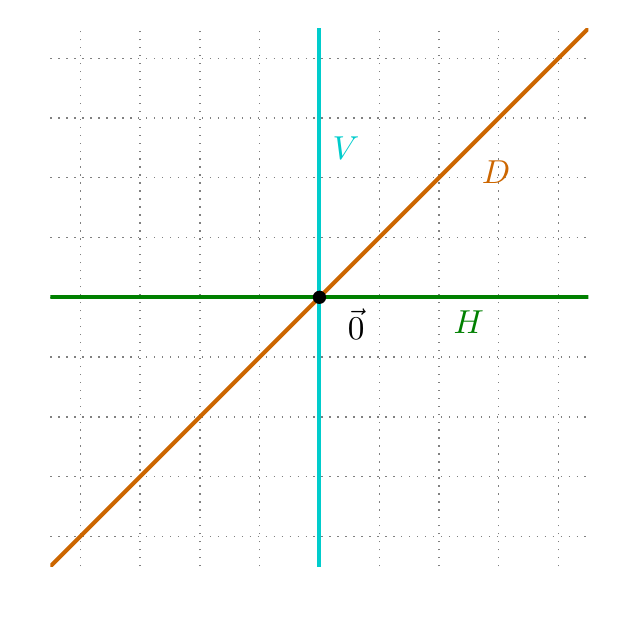
\begin{tikzpicture}[scale=1.2, >=latex]
    \begin{axis}[scale=1,
		    axis equal image,
		    axis line style={draw=none},
		    tick style={draw=none},
		    yticklabels={,,},
		    xticklabels={,,},
		 xmin=-4.5,
		 xmax=4.5,
		 ymin=-4.5,
		 ymax=4.5,
		 major grid style={dotted, gray},
                 xtick={-10,-9,...,10},
                 ytick={-10,-9,...,10},
                 grid=both,
		 anchor=origin]

	    \draw[Green, very thick] (-5,0) -- (5,0) node[near end, below] {$H$};
	    \draw[cyan!80!black, very thick] (0,-5) -- (0,5) node[near end, right] {$V$};
	    \draw[orange!80!black, very thick] (-5,-5) -- (5,5) node[near end, below right] {$D$};

	    \fill[fill=black] (0,0) circle[radius=2pt] node[below right, xshift=5pt] {\color{black}$\vec 0$};
    \end{axis}
\end{tikzpicture}
		\end{solution}
		\item $N=\Set*{\vec x\in\R^2 \given \vec x=t\mat{1\\1}\text{ for all }t\in\R}$.
				\begin{solution}[inline]
			$N=\Set{}$.
		\end{solution}

		\item $V\cup H$.
			\begin{solution}[inline]
			$V\cup H$ looks like a ``$+$'' going through the origin.
		\end{solution}
		\item $V\cap H$.
			\begin{solution}[inline]
				$V\cap H=\Set{\vec 0}$ is just the origin.
		\end{solution}
		\item Does $V\cup H=\R^2$?
			\begin{solution}
				No. $V\cup H$ does not contain $\mat{1\\1}$ while $\R^2$ does contain
				$\mat{1\\1}$.
			\end{solution}
	\end{parts}

	\begin{bookonly}\begin{center}\hspace{-2cm}\triplegrid\hspace{-2cm}\triplegrid\end{center}\end{bookonly}
	\bookonlynewpage
	\displayonlynewpage
\section*{Vector Combinations}
	\vspace{-1em}

	\SavedDefinitionRender{LinearCombination}

	\question
	\label{ProbSkewBasis}
	\begin{annotation}
		\begin{goals}
			\Goal{Practice linear combinations.}

			The goal of this problem is to
			\begin{itemize}
				\item Practice using the formal term \emph{linear combination}.
				\item Foreshadow span.
			\end{itemize}
		\end{goals}

		\begin{notes}
			\begin{itemize}
				\item In 2, the question should arise: ``Is $3\vec v_1$
					a linear combination of $\vec v_1$ \emph{and}
					$\vec v_2$?'' Address this.
				\item Refer to the magic carpet ride for 5. You don't
					need to do a full proof.
			\end{itemize}
		\end{notes}
	\end{annotation}
	Let $\vec v_1=\mat{1\\1}$, $\vec v_2=\mat{1\\-1}$, and $\vec w=2\vec v_1+\vec v_2$.
	\begin{parts}
		\item Write $\vec w$ as a column vector. When $\vec w$ is written as a
			linear combination of $\vec v_1$ and $\vec v_2$, what are the
			coefficients of $\vec v_1$ and $\vec v_2$?
			\begin{solution}
				$\vec w=\mat{3\\1}$; the coefficients are $(2,1)$.
			\end{solution}
		\item Is $\mat{3\\3}$ a linear combination of $\vec v_1$ and $\vec v_2$?
			\begin{solution}[inline]
				Yes. $\mat{3\\3}=3\vec v_1+0\vec v_2$.
			\end{solution}

		\item Is $\mat{0\\0}$ a linear combination of $\vec v_1$ and $\vec v_2$?
			\begin{solution}[inline]
				Yes. $\vec 0=0\vec v_1+0\vec v_2$.
			\end{solution}
		\item Is $\mat{4\\0}$ a linear combination of $\vec v_1$ and $\vec v_2$?
			\begin{solution}[inline]
				Yes. $\mat{4\\0}=2\vec v_1+2\vec v_2$.
			\end{solution}
		\item Can you find a vector in $\R^2$ that isn't a linear combination of
		$\vec v_1$ and $\vec v_2$?
			\begin{solution}
				No. $\mat{1\\0}=\tfrac{1}{2}\vec v_1+\tfrac{1}{2}\vec v_2$ and
				$\mat{0\\1}=\tfrac{1}{2}\vec v_1-\tfrac{1}{2}\vec v_2$.
				Therefore
				\[
					\mat{a\\b}
					= a\mat{1\\0}+b\mat{0\\1}
					= a(\tfrac{1}{2}\vec v_1+\tfrac{1}{2}\vec v_2)
						+b(\tfrac{1}{2}\vec v_1-\tfrac{1}{2}\vec v_2)
					=(\tfrac{a+b}{2})\vec v_1+(\tfrac{a-b}{2})\vec v_2.
				\]
				Therefore any vector in $\R^2$ can be written as linear combinations
				of $\vec v_1$ and $\vec v_2$.
			\end{solution}
		\item Can you find a vector in $\R^2$ that isn't a linear combination of
			$\vec v_1$?
			\begin{solution}
				Yes. All linear combinations of $\vec v_1$ have equal $x$ and
				$y$ coordinates, therefore $\vec w=\mat{2\\1}$ is not a linear
				combination of $\vec v_1$.
			\end{solution}
	\end{parts}


	\bookonlynewpage
	\question
	\begin{annotation}
		\begin{goals}
			\Goal{Practice formal writing.}
		\end{goals}

		\begin{notes}
			\begin{itemize}
				\item Make everyone \emph{write}. They will think
					they can do it, but they will find it hard if
					they try.
			\end{itemize}
		\end{notes}
	\end{annotation}
	Recall the \emph{Magic Carpet Ride} task where the hover board could
	travel in the direction $\vec h=\mat{3\\1}$ and the magic carpet could
	move in the direction $\vec m=\mat{1\\2}$.
	\begin{parts}
		\item Rephrase the sentence \emph{``Gauss can be reached using just the
			magic carpet and the hover board''} using formal mathematical
			language.
			\begin{solution}
				Gauss's location can be written as a linear combination of
				$\vec m$ and $\vec h$.
			\end{solution}
		\item Rephrase the sentence \emph{``There is nowhere Gauss can hide
			where he is inaccessible by magic carpet and hover board''} using
			formal mathematical language.
			\begin{solution}
				Every vector in $\R^2$ can be written as a linear combination
				of $\vec m$ and	$\vec h$.
			\end{solution}
		\item Rephrase the sentence \emph{``$\R^2$ is the set of all linear
			combinations of $\vec h$ and $\vec m$''} using formal mathematical
			language.
			\begin{solution}
				$\R^2=\Set{\vec v\given \vec v=t\vec m+s\vec h\text{ for some }t,s\in \R}$.
			\end{solution}
	\end{parts}

\begin{module}
	\Title{Sets of Vectors, Lines \& Planes}

	In this module you will learn
	\begin{itemize}
		\item How to draw a set of vectors making an appropriate choice of when to use
			line segments and when to use dots to represent vectors.
		\item The \emph{vector form} of lines and planes, including how to determine
			the intersection of lines and planes in vector form.
		\item Restricted linear combinations and how to use them to represent common geometric
			objects (like line segments or polygons).
	\end{itemize}

	\label{MODULELINESANDPLANES}
With a handle on vectors, we can now use them to describe some common geometric
objects: lines and planes.

\Heading{Lines}
Consider for a moment the line $\ell$ through the points $P$ and $Q$.  When $P,Q\in\R^2$, we
can describe $\ell$ with an equation of the form $y=mx+b$ (provided it isn't a vertical line), but if
$P,Q\in\R^3$, it's much harder to describe $\ell$ with an equation. We can solve this problem by using vectors. 

Let $\vec d=\overrightarrow{PQ}$ and consider the set of points (or vectors) $\vec x$ that can be expressed as
\[
	\vec x=t\vec d+P
\]
for $t\in \R$.  Geometrically, this is the set of all points we get by starting at $P$ and
displacing by some multiple of $\vec d$.  This is a line!


\begin{center}
	\begin{tikzpicture}
		\coordinate (A) at (1,1);
		\coordinate (B) at (3,2);
		\coordinate (D) at ($(B)-(A)$);
		\begin{axis}[
		    anchor=origin,
		    disabledatascaling,
		    xmin=-1,xmax=5,
		    ymin=-1,ymax=3,
		    x=1cm,y=1cm,
		    grid=both,
		    grid style={line width=.1pt, draw=gray!10},
		    %major grid style={line width=.2pt,draw=gray!50},
		    axis lines=middle,
		    minor tick num=0,
		    enlargelimits={abs=0.5},
		    axis line style={latex-latex},
		    ticklabel style={font=\tiny,fill=white},
		    xlabel style={at={(ticklabel* cs:1)},anchor=north west},
		    ylabel style={at={(ticklabel* cs:1)},anchor=south west}
		]

		\draw [Green,fill] (A) circle[radius=1.5pt] node [below right] {$P$};
		\draw [Green,fill] (B) circle[radius=1.5pt] node [below right] {$Q$};
		\draw[->,thick,myred!60!white] (A) -- (B) node [midway,below right,yshift=2pt] {$\vec d$};


		\end{axis}
		\foreach \x in {-1,5} {
			\draw [mypink,fill] ($(A)+\x/3*(D)$) circle[radius=1.5pt] node [left] {\footnotesize$\tfrac{\x}{3}\vec d+P$};
		}
		\foreach \x in {-3,-2,4,6} {
			\draw [mypink,fill] ($(A)+\x/3*(D)$) circle[radius=1.5pt];
		}
	\end{tikzpicture}
	\begin{tikzpicture}
		\coordinate (A) at (1,1);
		\coordinate (B) at (3,2);
		\coordinate (D) at ($(B)-(A)$);
		\begin{axis}[
		    anchor=origin,
		    disabledatascaling,
		    xmin=-1,xmax=5,
		    ymin=-1,ymax=3,
		    x=1cm,y=1cm,
		    grid=both,
		    grid style={line width=.1pt, draw=gray!10},
		    %major grid style={line width=.2pt,draw=gray!50},
		    axis lines=middle,
		    minor tick num=0,
		    enlargelimits={abs=0.5},
		    axis line style={latex-latex},
		    ticklabel style={font=\tiny,fill=white},
		    xlabel style={at={(ticklabel* cs:1)},anchor=north west},
		    ylabel style={at={(ticklabel* cs:1)},anchor=south west}
		]

		\draw [Green,fill] (A) circle[radius=1.5pt] node [below right] {$P$};
		\draw [Green,fill] (B) circle[radius=1.5pt] node [below right] {$Q$};
		\draw[->,thick,myred!60!white] (A) -- (B) node [midway,below right,yshift=2pt] {$\vec d$};

		\end{axis}

		\foreach \x in {-3,-2,-1,0,4,5,6} {
			\draw [->, gray!50!white] (0,0) -- ($(A)+\x/3*(D)$);
		}
		\foreach \x in {-1,5} {
			\draw [mypink,fill] ($(A)+\x/3*(D)$) circle[radius=1.5pt] node [left] {\footnotesize$\tfrac{\x}{3}\vec d+P$};
		}
		\foreach \x in {-3,-2,4,6} {
			\draw [mypink,fill] ($(A)+\x/3*(D)$) circle[radius=1.5pt];
		}
	\end{tikzpicture}
\end{center}
We simultaneously interpret this line as a set of points (the points that make up
the line) and as a set of vectors 
rooted at the origin (the vectors pointing from the origin to the line).
Note that sometimes we draw vectors as directed line segments.
Other times, we draw
each vector by marking only its ending point because drawing each vector as a line segment
would make
it hard to see what is going on.

Which picture below do you think best represents $\ell$?
\begin{center}
	\begin{tikzpicture}
		\coordinate (A) at (1,1);
		\coordinate (B) at (3,2);
		\coordinate (D) at ($(B)-(A)$);
		\begin{axis}[
		    anchor=origin,
		    disabledatascaling,
		    xmin=-1,xmax=5,
		    ymin=-1,ymax=3,
		    x=1cm,y=1cm,
		    grid=both,
		    grid style={line width=.1pt, draw=gray!10},
		    %major grid style={line width=.2pt,draw=gray!50},
		    axis lines=middle,
		    minor tick num=0,
		    enlargelimits={abs=0.5},
		    axis line style={latex-latex},
		    ticklabel style={font=\tiny,fill=white},
		    xlabel style={at={(ticklabel* cs:1)},anchor=north west},
		    ylabel style={at={(ticklabel* cs:1)},anchor=south west}
		]

		\node[above right] at (0,3) {~Vectors in $\ell$ as dots};
		\draw [mypink, thick] ($(A)-3*(D)$) -- ($(A)+3*(D)$);
		\end{axis}
	\end{tikzpicture}
	\begin{tikzpicture}
		\coordinate (A) at (1,1);
		\coordinate (B) at (3,2);
		\coordinate (D) at ($(B)-(A)$);
		\begin{axis}[
		    anchor=origin,
		    disabledatascaling,
		    xmin=-1,xmax=5,
		    ymin=-1,ymax=3,
		    x=1cm,y=1cm,
		    grid=both,
		    grid style={line width=.1pt, draw=gray!10},
		    %major grid style={line width=.2pt,draw=gray!50},
		    axis lines=middle,
		    minor tick num=0,
		    enlargelimits={abs=0.5},
		    axis line style={latex-latex},
		    ticklabel style={font=\tiny,fill=white},
		    xlabel style={at={(ticklabel* cs:1)},anchor=north west},
		    ylabel style={at={(ticklabel* cs:1)},anchor=south west}
		]
			\node[above right] at (0,3) {~Vectors in $\ell$ as arrows from $(0,0)$};
		\end{axis}

		\foreach \x in {-8,...,14} {
			\draw [->, mypink] (0,0) -- ($(A)+\x/6*(D)$);
		}
	\end{tikzpicture}
\end{center}


\begin{emphbox}[Takeaway]
	When drawing a picture depicting several vectors, make an appropriate choice (arrows, dots, or
	a mix) so that the picture is clear.
\end{emphbox}

The line $\ell$ described above can be written in set-builder notation
as:
\[
	\ell=\Set{\vec x\given \vec x=t\vec d+P\text{ for some }t\in \R}.
\]
Notice that in set-builder notation, we write ``for some $t\in \R$.'' Make sure you
understand why replacing ``for some $t\in\R$'' with ``for
all $t\in \R$'' would be incorrect.

\medskip
Writing lines with set-builder notation all the time can be overkill,
so we will allow ourselves to describe lines in a shorthand called \emph{vector form}\footnote{
	$y=mx+b$ form of a line is also shorthand.  The line $\ell$ described by the equation
	$y=mx+b$ is actually the set $\Set{(x,y)\in\R^2\given y=mx+b}$.
}.

\SavedDefinitionRender{VectorFormofaLine}

We can also use coordinates when writing a line in vector form. For example,
\[
	\mat{x\\y}=t\mat{d_1\\d_2}+\mat{p_1\\p_2}
\]
corresponds to the line passing through $\mat{p_1\\p_2}$ with $\mat{d_1\\d_2}$ as a direction vector.

The ``$t$'' that appears in a vector form is called the \emph{parameter variable}\index[definitions]{Parameter variable}\index{Parameter variable}, and for this
reason, some textbooks use the term \emph{parametric form} in place of ``vector form''. 

\medskip
Writing a line in vector form requires only a point on the line and a direction for the line\footnote{ Notice that
a direction vector \emph{for} a line $\ell$ is different than a vector \emph{in} a line $\ell$.},
which makes converting from another form into vector form straightforward.
\begin{example}
	Find vector form of the line $\ell\subseteq\R^2$ with equation $y=2x+3$.

	First, we find two
	points on $\ell$.  By guess-and-check, we see $P=(0,3)$ and $Q=(1,5)$ are on $\ell$.
	Thus, a direction vector for $\ell$ is given by
	\[
		\vec d = \mat{1\\5}-\mat{0\\3}=\mat{1\\2}.
	\]
	We may now express $\ell$ in vector form as
	\[
		\vec x=t\vec d+P
	\]
	or, using coordinates, as
	\[
		\mat{x\\y} = t\mat{1\\2}+\mat{0\\3}.
	\]
\end{example}

It's important to note that when we write a line in vector form, it is a \emph{specific shorthand} notation.
If we augment the notation, we no longer have written a line in ``vector form''.

\begin{example} Let $\ell$ be a line, let $\vec d$ be a direction vector for $\ell$, and let $\vec p\in \ell$
	be a point on $\ell$. Writing
	\[
		\vec x=t\vec d+\vec p
	\]
	or 
	\[
		\vec x=t\vec d+\vec p\quad\text{ where }\quad t\in \R
	\]
	specifies $\ell$ in vector form; both are shorthands for $\Set{\vec x\given
	\vec x=t\vec d+\vec p\text{ for some }t\in \R}$. But,
	\[
		\vec x=t\vec d+\vec p\quad\text{ for some }\quad t\in \R
	\]
	and
	\[
		\vec x=t\vec d+\vec p\quad\text{ for all }\quad t\in \R
	\]
	are logical statements about the vectors $\vec x$, $\vec d$, and
	$\vec p$. These statements are either true or false; they do \emph{not} 
	specify $\ell$ in vector form.

	Similarly, the statement
	\[
		\ell = t\vec d+\vec p
	\]
	is mathematically nonsensical and does not specify $\ell$ in vector form. (On the
	left is a \emph{set} and on the right is a \emph{vector}!)

\end{example}

\begin{emphbox}[Takeaway]
	Vector form is a specific shorthand for a set. If ``extra'' words or symbols are added
	to the vector form, it stops being a shorthand.
\end{emphbox}

But, why is vector form useful? For starters, every line can be expressed in vector form 
(you cannot write a vertical line in $y=mx+b$ form, and in $\R^3$, you would need two linear equations
to represent a line). But, the most useful thing about expressing a line in vector form is that
you can easily generate points on that line.

Suppose $\ell$ can be represented in vector form as $\vec x=t\vec d+\vec p$.
Then, for every $t\in \R$, the vector $t\vec d +\vec p\in\ell$. Not only that, but as $t$ ranges over
$\R$, all points on $\ell$ are ``traced out''. Thus, we can find points on $\ell$ without having to ``solve''
any equations.

The downside to using vector form is that it is not unique. There are multiple direction vectors and multiple points
for every line.  Thus, merely by looking at the vector equation for two lines, it can be hard to tell if
they're equal.

For example,
\[
	\mat{x\\y} = t\mat{1\\2}+\mat{0\\3},\qquad
	\mat{x\\y} = t\mat{2\\4}+\mat{0\\3},\quad\text{and}\quad
	\mat{x\\y} = t\mat{1\\2}+\mat{1\\5}
\]
all represent the same line.  In the second equation, the direction vector is parallel but scaled, and in
the third equation, a different point on the line was chosen.

Recall that in vector form, the variable $t$ is called the \emph{parameter variable}.  It is an instance of
a \emph{dummy variable}. In other words, $t$ is a placeholder---just because ``$t$'' appears in two different vector
forms, doesn't mean it's the same quantity.

To drive this point home, let's think about vector form in terms
of the sets it specifies. Let $\vec d_1,\vec d_2\neq\vec 0$ and $\vec p_1,\vec p_2$ be vectors and define the lines
\[
	\ell_1=\Set{\vec x\given \vec x=t\vec d_1+\vec p_1\text{ for some }t\in\R}
\]
and
\[
	\ell_2=\Set{\vec x\given \vec x=t\vec d_2+\vec p_2\text{ for some }t\in\R}.
\]
These lines have vector forms $\vec x=t\vec d_1+\vec p_1$ and $\vec x=t\vec d_2+\vec p_2$.
However, declaring that $\ell_1=\ell_2$ if and only if $t\vec d_1+\vec p_1=t\vec d_2+\vec p_2$
does \emph{not} make sense.   Instead, as per the definition, $\ell_1=\ell_2$ if $\ell_1\subseteq\ell_2$ and $\ell_2\subseteq\ell_1$.
If $\vec x\in\ell_1$ then $\vec x=t\vec d_1+\vec p_1$ for some $t\in\R$.  If $\vec x\in\ell_2$
then $\vec x=t\vec d_2+\vec p_2$ for some \emph{possibly different} $t\in \R$.  This can get
confusing really quickly.  The easiest way to avoid confusion is to use different parameter variables 
when comparing different vector forms.

\begin{example}
	Determine if the lines $\ell_1$ and $\ell_2$, given in vector form as 
	\[
		\vec x=t\mat{1\\1}+\mat{2\\1}\qquad\text{and}\qquad
		\vec x=t\mat{2\\2}+\mat{4\\3},
	\]
	are the same line.  
	
	To determine this, we need to figure out if $\vec x\in\ell_1$
	implies $\vec x\in \ell_2$ and if $\vec x\in\ell_2$ implies $\vec x\in\ell_1$.

	If $\vec x\in\ell_1$, then $\vec x=t\mat{1\\1}+\mat{2\\1}$ for some $t\in\R$.  If
	$\vec x\in\ell_2$, then $\vec x=s\mat{2\\2}+\mat{4\\3}$ for some $s\in \R$.  Thus if
	\[
		t\mat{1\\1}+\mat{2\\1} = \vec x = s\mat{2\\2}+\mat{4\\3}
	\]
	always has a solution, $\ell_1=\ell_2$.  Moving everything to one side, we see
	\begin{align*}
		\vec 0 = \mat{4\\3}-\mat{2\\1} + s\mat{2\\2}-t\mat{1\\1}
		&=\mat{2\\2}+s\mat{2\\2}-t\mat{1\\1}\\
		&=(s+1)\mat{2\\2}-\tfrac{t}{2}\mat{2\\2}\\
		&= (s+1-\tfrac{t}{2})\mat{2\\2}.
	\end{align*}
	This equation has a solution whenever $s+1-t/2=0$ has a solution.  Since for every $s$, the
	equation $s+1-t/2=0$ has a solution, and for every $t$, the equation $s+1-t/2=0$ has a solution,
	we know $\ell_1=\ell_2$.
\end{example}


\Heading{Vector Form in Higher Dimensions}
The geometry of lines in space ($\R^3$ and above) is a bit more complicated than that of lines
in the plane.  Lines in the plane either intersect or are parallel.
In space,  we have to be careful about what we mean by
``parallel lines,'' since lines with entirely different directions can
still fail to intersect\footnote{ Recall that in Euclidean geometry
two lines are defined to be parallel if they coincide or never intersect.}.

\begin{center}
  \begin{tikzpicture}
    \begin{axis}[grid=major,view={20}{40},z buffer=sort,
	    zmin=0,
	    xticklabels={,,}, yticklabels={,,}, zticklabels={,,}
	    ]
	    \addplot3 [no marks,orange,ultra thick] coordinates {(0,10,10) (20,10,30)};
	    \addplot3 [no marks,orange,dashed, thick] coordinates {(0,10,0) (20,10,0)};
	    \addplot3 [no marks,mypink,ultra thick] coordinates {(0,0,20) (20,20,0)};
	    \addplot3 [no marks,mypink,dashed, thick] coordinates {(0,0,0) (20,20,0)};
	%\addplot3[domain=4:30,samples=80,samples y=0,mark=none,orange, opacity=0.5,ultra thick]
	%    ({x},{118.89/x},{2*x});
    \end{axis}
  \end{tikzpicture}
\end{center}

\begin{example}
Consider the lines described by
\begin{align*}
\vec x &= t( 1, 3, -2 ) + ( 1, 2, 1 ) \\
\vec x &= t( -2, -6, 4) + ( 3, 1, 0 ).
\end{align*}
They have parallel directions since $( -2, -6, 4 ) = -2( 1, 3,-2 )$.
Hence, in this case, we say the lines are \emph{parallel}\index{Line!parallel}.  (How can
we be sure the lines are not the same?)
\end{example}

\begin{example}
Consider the lines described by
\begin{align*}
	\vec x &= t(1, 3, -2 ) + ( 1, 2, 1 ) \\
	\vec x &= t( 0, 2, 3) + ( 0, 3, 9 ).
\end{align*}
They are not parallel because neither of the direction
vectors is a multiple
of the other.  They may or may not intersect.  (If they don't,
	we say the lines are \emph{skew}\index{Line!skew}.)  How can we find out?
	Mirroring our earlier approach,
	we can set their equations equal and see if we can solve for a point
	of intersection \emph{after ensuring we give their parametric variables
	different names}.   We'll keep one parametric variable named $t$ and name the
	other one $s$.  Thus, we want
\[
\vec x = t( 1, 3, -2 ) + ( 1, 2, 1 ) =
s( 0, 2, 3) + ( 0, 3, 9 ),
\]
which after collecting terms yields
\[
    ( t + 1, 3t + 2, -2t + 1 ) = ( 0, 2s + 3, 3s + 9).
\]
Reading coordinate by coordinate, we get three equations
\begin{align*}
    t + 1 &= 0 \\
    3t +2 &= 2s + 3 \\
    -2t + 1 &=  3s + 9
\end{align*}
in two unknowns  $s$ and $t$.  This is an {\it overdetermined\/}
system\index{System of linear equations!overdetermined system}, and it may or may not have a solution.
The first two equations yield $t = -1$  and $s = -2$.  Putting
these values in the last equation yields $(-2)(-1) + 1 = 3(-2) + 9$,
which is indeed true.
Hence, the equations are consistent, and the lines
intersect.   To find the point of intersection, put $t = -1$
in the equation for the vector equation of the first line (or
$s = -2$ in that for the second) to obtain  $( 0, -1, 3 )$.
\end{example}

\Heading{Planes}

Any two distinct points define a line.  To define a plane, we
need three points.  But there's a caveat: the three points cannot
be on the same line, otherwise they'd define a line
and not a plane.  Let $A,B,C\in\R^3$ be three points that are not
collinear and let $\mathcal P$ be the plane that passes through $A$,
$B$, and $C$.

Just like lines, planes have direction vectors.  For $\mathcal P$, both
$\vec d_1=\overrightarrow{AB}$ and $\vec d_2=\overrightarrow{AC}$ are direction
vectors.  Of course, $\vec d_1$, $\vec d_2$ and their multiples
are not the only direction vectors for $\mathcal P$. There are infinitely many more, including
$\vec d_1+\vec d_2$, and $\vec d_1-7\vec d_2$, and so on.  However, since a plane
is a \emph{two}-dimensional object, we only need two different direction vectors to describe it.

Like lines, planes have a vector form.  Using the direction vectors $\vec d_1=\overrightarrow{AB}$ and 
$\vec d_2=\overrightarrow{AC}$,
the plane $\mathcal P$ can be written in vector form as
\[
	\mat{x\\y\\z} = t\vec d_1+s\vec d_2+A.
\]
\begin{center}
  \begin{tikzpicture}
    \begin{axis}[grid=major,view={20}{40},z buffer=sort,
	    %zmin=0,
	    xticklabels={,,}, yticklabels={,,}, zticklabels={,,}
	    ]
		\addplot3 [data cs=cart,surf,domain=-10:10,samples=2, opacity=0.5]
		{x+y};
		\coordinate (A) at (axis cs:-3,-3,-6);
		\coordinate (B) at (axis cs:3,4,7);
		\coordinate (C) at (axis cs:-4,4,0);

		\draw [mypink,fill] (A) circle[radius=1.5pt] node [below right] {$A$};
		\draw [->, thick] (A) -- (B) node [midway,below right] {$\vec d_1$};
		\draw [->, thick] (A) -- (C) node [midway,above left] {$\vec d_2$};
    \end{axis}
  \end{tikzpicture}
\end{center}

\SavedDefinitionRender{VectorFormofaPlane}

\begin{example}
	Describe the plane $\mathcal P\subseteq \R^3$ with equation $z=2x+y+3$ in vector form.

	To describe $\mathcal P$ in vector form, we need a point on $\mathcal P$ and two direction
	vectors for $\mathcal P$. By guess-and-check, we see the points
	\[
		A=\mat{0\\0\\3}\qquad B=\mat{1\\0\\5}\qquad C=\mat{0\\1\\4}
	\]
	are all in $\mathcal P$. Thus
	\[
		\vec d_1=B-A=\mat{1\\0\\2}\qquad \text{and}\qquad
		\vec d_2=C-A=\mat{0\\1\\1}
	\]
	are both direction vectors for $\mathcal P$.  Since these vectors are not parallel, 
	we can express $\mathcal P$ in vector
	form as
	\[
		\vec x=t\vec d_1+s\vec d_2+A=t\mat{1\\0\\2}+s\mat{0\\1\\1}+\mat{0\\0\\3}.
	\]
\end{example}


\begin{example}
	Find the line of intersection between $\mathcal P_1$ and $\mathcal P_2$ where the planes
	are given in vector form by
	\[
		\overbrace{\vec x=t\mat{1\\1\\0}+s\mat{-1\\0\\1}+\mat{1\\2\\3}}^{\displaystyle\mathcal P_1}
		\qquad\text{and}\qquad
		\overbrace{\vec x=t\mat{-1\\0\\2}+s\mat{1\\2\\1}+\mat{0\\0\\3}}^{\displaystyle\mathcal P_2}.
	\]

	Just like in the example for lines, we are looking for points $\vec x$ that are in both planes. To
	keep from getting mixed up, we'll use $a$, $b$, $c$, and $d$ as parameter variables. Therefore, we are looking
	for solutions to
	\[
		a\mat{1\\1\\0}+b\mat{-1\\0\\1}+\mat{1\\2\\3}=\vec x=c\mat{-1\\0\\2}+d\mat{1\\2\\1}+\mat{0\\0\\3}.
	\]
	Collecting terms, this is equivalent to the system of equations
	\[
		\systeme{a-b+c-d=-1,a-2d=-2,b-2c-d=0}.
	\]
	This system is underdetermined (there are four variables and three equations). If $\mathcal P_1$ 
	and $\mathcal P_2$ indeed intersect in a line, we know there must an infinite number
	of solutions to this system. After row reducing\footnote{ See Appendix \ref{APPSLEI}, System \eqref{EQVECEQ2} and \eqref{EQEQUIVSYS}.}, we see
	\[
		\mat{a\\b\\c\\d} = \matc{r\\r/2-1\\-1\\r/2+1}
	\]
	is a solution for every $r\in\R$. We can substitute these parameters into either of the original equations
	to get an equation for the line of intersection. Picking the second one, we see
	\[
		\vec x=c\mat{-1\\0\\2}+d\mat{1\\2\\1}+\mat{0\\0\\3}=-\mat{-1\\0\\2}+(\tfrac{r}{2}+1)\mat{1\\2\\1}+\mat{0\\0\\3}
		=\tfrac{r}{2}\mat{1\\2\\1}+\mat{2\\2\\2}
	\]
	is in both planes for every $r\in \R$. Therefore, we may express $\mathcal P_1\cap \mathcal P_2$ in vector form as
	\[
		\vec x=r\matc{1/2\\1\\1/2}+\mat{2\\2\\2}.
	\]
\end{example}

\Heading{Restricted Linear Combinations}

Using vectors, we can describe more than just lines and planes---we can describe 
all sorts of geometric objects.

Recall that when we write $\vec x=t\vec d+\vec p$
to describe the line $\ell$,
what we mean is
\[
	\ell=\Set{\vec x\given \vec x=t\vec d+\vec p\text{ for some }t\in \R}.
\]
The line $\ell$ stretches off infinitely in both directions. But, what if we wanted
to describe just a part of $\ell$? We can do this by placing additional restrictions
on $t$.
For example, consider the ray $R$
and the line segment $S$:
\begin{align*}
	R&=\Set{\vec x\given \vec x=t\vec d+\vec p\text{ for some }t\geq 0}\\
	S&=\Set{\vec x\given \vec x=t\vec d+\vec p\text{ for some }t\in [0,2]}
\end{align*}

\begin{center}
	\begin{tikzpicture}
		\begin{axis}[
		    anchor=origin,
		    disabledatascaling,
		    xmin=-1,xmax=4,
		    ymin=-1,ymax=3,
		    x=1cm,y=1cm,
		    grid=both,
		    grid style={line width=.1pt, draw=gray!10},
			xtick={0,1,2,3,4},
		    %major grid style={line width=.2pt,draw=gray!50},
		    axis lines=middle,
		    minor tick num=0,
		    enlargelimits={abs=0.5},
		    axis line style={latex-latex},
		    ticklabel style={font=\tiny,fill=white},
		    xlabel style={at={(ticklabel* cs:1)},anchor=north west},
		    ylabel style={at={(ticklabel* cs:1)},anchor=south west}
		]

			\draw [mypink, very thick] (0,0) -- (5,3) node[midway, below right] {$R$};
			\draw [black!70!white, thick,dashed, ->, yshift=.15cm] (0,0) -- (5/5,3/5) node[midway, above] {$\vec d$};
		\end{axis}
			\node[above right] at (0,3) {~The ray $R$};
	\end{tikzpicture}
	~~~~
	\begin{tikzpicture}
		\begin{axis}[
		    anchor=origin,
		    disabledatascaling,
		    xmin=-1,xmax=4,
		    ymin=-1,ymax=3,
			xtick={0,1,2,3,4},
		    x=1cm,y=1cm,
		    grid=both,
		    grid style={line width=.1pt, draw=gray!10},
		    %major grid style={line width=.2pt,draw=gray!50},
		    axis lines=middle,
		    minor tick num=0,
		    enlargelimits={abs=0.5},
		    axis line style={latex-latex},
		    ticklabel style={font=\tiny,fill=white},
		    xlabel style={at={(ticklabel* cs:1)},anchor=north west},
		    ylabel style={at={(ticklabel* cs:1)},anchor=south west}
		]
			\draw [mygreen, very thick] (0,0) -- (10/5,6/5) node[midway, below right] {$S$};
			\draw [black!70!white, thick,dashed, ->, yshift=.15cm] (0,0) -- (5/5,3/5) node[midway, above] {$\vec d$};
		\end{axis}
			\node[above right] at (0,3) {~The line segment $S$};
	\end{tikzpicture}
\end{center}

We can also make polygons by adding restrictions to the vector form of a plane. Let
$\vec a=\mat{2\\1}$ and $\vec b=\mat{-1\\1}$ and consider the unit square $U$ and
the parallelogram $P$ defined by
\begin{align*}
	U&=\Set{\vec x\given \vec x=t\xhat+s\yhat\text{ for some }t,s\in [0,1]}\\
	P&=\Set{\vec x\given \vec x=t\vec a+s\vec b\text{ for some }t\in [0,1]\text{ and }s\in[-1,1]}
\end{align*}

\begin{center}
	\begin{tikzpicture}
		\begin{axis}[
		    anchor=origin,
		    disabledatascaling,
		    xmin=-2,xmax=3,
		    ymin=-1,ymax=2,
			xtick={-2,...,3},
			ytick={-2,...,3},
		    x=1cm,y=1cm,
		    grid=both,
		    grid style={line width=.1pt, draw=gray!10},
		    %major grid style={line width=.2pt,draw=gray!50},
		    axis lines=middle,
		    minor tick num=0,
		    enlargelimits={abs=0.5},
		    axis line style={latex-latex},
		    ticklabel style={font=\tiny,fill=white},
		    xlabel style={at={(ticklabel* cs:1)},anchor=north west},
		    ylabel style={at={(ticklabel* cs:1)},anchor=south west}
		]

			\fill [mypink, opacity=.3] (0,0) -- (1,0) -- (1,1) node[midway, right, opacity=1] {$U$} -- (0,1) -- cycle;
			\draw [black!70!white, thick,dashed, ->, yshift=-.15cm] (0,0) -- (1,0) node[midway, below] {$\xhat$};
			\draw [black!70!white, thick,dashed, ->, xshift=-.15cm] (0,0) -- (0,1) node[midway, left] {$\yhat$};
		\end{axis}
			\node[above right] at (0,2) {~The unit square $U$};
	\end{tikzpicture}
	~~~~
	\begin{tikzpicture}
		\begin{axis}[
		    anchor=origin,
		    disabledatascaling,
		    xmin=-2,xmax=3,
		    ymin=-1,ymax=2,
			xtick={-2,...,3},
			ytick={-2,...,3},
		    x=1cm,y=1cm,
		    grid=both,
		    grid style={line width=.1pt, draw=gray!10},
		    %major grid style={line width=.2pt,draw=gray!50},
		    axis lines=middle,
		    minor tick num=0,
		    enlargelimits={abs=0.5},
		    axis line style={latex-latex},
		    ticklabel style={font=\tiny,fill=white},
		    xlabel style={at={(ticklabel* cs:1)},anchor=north west},
		    ylabel style={at={(ticklabel* cs:1)},anchor=south west}
		]
			\fill [mygreen, opacity=.3] (1,2) -- (3,0) -- (1,-1) node[midway, below right, opacity=1] {$P$} -- (-1,1) -- cycle;
			\draw [black!70!white, thick,dashed, ->] (0,0) -- (2,1) node[midway, below right] {$\vec a$};
			\draw [black!70!white, thick,dashed, ->] (0,0) -- (-1,1) node[midway, left, yshift=-3pt] {$\vec b$};
		\end{axis}
			\node[above right] at (0,2) {~The parallelogram $P$};
	\end{tikzpicture}
\end{center}

Each set so far is a set of linear combinations, and we 
have made different shapes by restricting the coefficients of those linear
combinations. There are two ways of restricting linear combinations that arise
often enough to get their own names.

\SavedDefinitionRender{NonnegativeConvexLinearCombinations}

You can think of non-negative linear combinations as vectors you can arrive at by
only displacing ``forward''.
Convex linear combinations can be thought of as weighted averages of vectors (the average of $\vec v_1,\ldots,
\vec v_n$ would be the convex linear combination with coefficients $\alpha_i=\frac{1}{n}$). 
A convex linear combination
of two vectors gives a point on the line segment connecting them. 

\begin{example}
	Let $\vec a=\mat{2\\1}$ and $\vec b=\mat{1\\-1}$ and define
	\begin{align*}
		A&=\Set{\vec x\given \vec x\text{ is a convex linear combination of }\vec a\text{ and }\vec b}\\
		&=\Set{\vec x\given \vec x=\alpha\vec a+(1-\alpha)\vec b\text{ for some }\alpha\in [0,1]}.
	\end{align*}
	Draw $A$.

	We know $\vec x=\alpha\vec a+(1-\alpha)\vec b\in A$ whenever $\alpha\in[0,1]$. If we rearrange the
	equation $\vec x=\alpha\vec a+(1-\alpha)\vec b$, we see
	\[
		\vec x=\alpha\vec a-\alpha\vec b+\vec b = \alpha(\vec a-\vec b)+\vec b,
	\]
	which looks like the vector form of a line which passes through $\vec b$ with direction $\vec a-\vec b$.
	However, we have the additional restriction $\alpha\in[0,1]$, so $A$ is only the part of that line which connects $\vec a$
	and $\vec b$.

\begin{center}
	\begin{tikzpicture}
	\tikzset{test/.style n args={3}{
	    postaction={
	    decorate,
	    decoration={
	    markings,
	    mark=between positions 0 and \pgfdecoratedpathlength step 0.5pt with {
	    \pgfmathsetmacro\myval{multiply(
		divide(
		\pgfkeysvalueof{/pgf/decoration/mark info/distance from start}, \pgfdecoratedpathlength
		),
		100
	    )};
	    \pgfsetfillcolor{#3!\myval!#2};
	    \pgfpathcircle{\pgfpointorigin}{#1};
	    \pgfusepath{fill};}
	}}}}
		\begin{axis}[
		    anchor=origin,
		    name=plot1,
		    disabledatascaling,
		    xmin=-1,xmax=3,
		    ymin=-1,ymax=2,
			xtick={-4,...,4},
			ytick={-2,...,4},
		    x=1cm,y=1cm,
		    grid=both,
		    grid style={line width=.1pt, draw=black!10},
		    %major grid style={line width=.2pt,draw=gray!50},
		    axis lines=middle,
		    minor tick num=0,
		    enlargelimits={abs=0.5},
		    axis line style={latex-latex},
		    ticklabel style={font=\tiny,fill=\currentbackgroundcolor},
		    xlabel style={at={(ticklabel* cs:1)},anchor=north west},
		    ylabel style={at={(ticklabel* cs:1)},anchor=south west}
		]
			\coordinate (A) at (2,1);
			\coordinate (B) at (1,-1);
			\coordinate (C) at ($.3*(A)+.7*(B)$);
			\coordinate (D) at ($.7*(A)+.3*(B)$);
			%\fill[mypink] (A) circle[radius=2pt] node[above right] {$\vec a$};
			%\fill[mygreen] (B) circle[radius=2pt] node[above right] {$\vec b$};
			\draw[thick, mypink, ->] (0,0) -- (A) ;
			\draw[thick, mypink!30!mygreen, ->] (0,0) -- (C) ;
			\draw[thick, mypink!70!mygreen, ->] (0,0) -- (D) ;
			\draw[thick, mygreen, ->] (0,0) -- (B);
		\end{axis}
		\node[right, mypink] at (A) {\small$\vec a=1\vec a+(1-1)\vec b$};
		\node[right, mypink!30!mygreen] at (C) {\small$\tfrac{1}{3}\vec a+(1-\tfrac{1}{3})\vec b$};
		\node[right, mypink!70!mygreen] at (D) {\small$\tfrac{2}{3}\vec a+(1-\tfrac{2}{3})\vec b$};
		\node[right, mygreen] at (B) {\small$\vec b=0\vec a+(1-0)\vec b$};
	\end{tikzpicture}
	\begin{tikzpicture}
	\tikzset{test/.style n args={3}{
	    postaction={
	    decorate,
	    decoration={
	    markings,
	    mark=between positions 0 and \pgfdecoratedpathlength step 0.5pt with {
	    \pgfmathsetmacro\myval{multiply(
		divide(
		\pgfkeysvalueof{/pgf/decoration/mark info/distance from start}, \pgfdecoratedpathlength
		),
		100
	    )};
	    \pgfsetfillcolor{#3!\myval!#2};
	    \pgfpathcircle{\pgfpointorigin}{#1};
	    \pgfusepath{fill};}
	}}}}
		\begin{axis}[
		    anchor=origin,
		    name=plot1,
		    disabledatascaling,
		    xmin=-1,xmax=3,
		    ymin=-1,ymax=2,
			xtick={-4,...,4},
			ytick={-2,...,4},
		    x=1cm,y=1cm,
		    grid=both,
		    grid style={line width=.1pt, draw=black!10},
		    %major grid style={line width=.2pt,draw=gray!50},
		    axis lines=middle,
		    minor tick num=0,
		    enlargelimits={abs=0.5},
		    axis line style={latex-latex},
		    ticklabel style={font=\tiny,fill=\currentbackgroundcolor},
		    xlabel style={at={(ticklabel* cs:1)},anchor=north west},
		    ylabel style={at={(ticklabel* cs:1)},anchor=south west}
		]
			\coordinate (A) at (2,1);
			\coordinate (B) at (1,-1);
			\coordinate (C) at ($.3*(A)+.7*(B)$);
			\coordinate (D) at ($.7*(A)+.3*(B)$);
			\fill[mypink] (A) circle[radius=2pt];
			\fill[mygreen] (B) circle[radius=2pt];
			%\draw[thick, mypink, ->] (0,0) -- (A) ;
			%\draw[thick, mypink!30!mygreen, ->] (0,0) -- (C) ;
			%\draw[thick, mypink!70!mygreen, ->] (0,0) -- (D) ;
			%\draw[thick, mygreen, ->] (0,0) -- (B) node[below right] {$\vec b=0\vec a+(1-0)\vec b$};
		\end{axis}
		\draw [test={0.8pt}{mypink}{mygreen}, thick] (A) to node[midway, above left, mygreen!40!mypink] {$A$}(B) ;
		\node[above right, mypink] at (A) {$\vec a$};
		\node[below right, mygreen] at (B) {$\vec b$};
	\end{tikzpicture}
\end{center}
Since $A$ is an infinite collection of vectors, it's better to draw vectors in $A$ as dots rather than lines from the origin.
\end{example}


	\begin{exercises}
	\begin{problist}
		\prob  Express the following lines in vector form.
		\begin{enumerate}
			\item   $\ell_1\subseteq\R^2$ with equation $4x-3y=-10$.
			\item   $\ell_2\subseteq\R^2$ which passes through the points $A=(1,1)$ and $B=(2,7)$.
			\item   $\ell_3\subseteq\R^2$ which passes through $\vec 0$ and is parallel to the line
				with equation $4x-3y=-10$.
			\item   $\ell_4\subseteq\R^3$ which passes through the points $A=(-1,-1,0)$ and $B=(2,3,5)$.
			\item   $\ell_5\subseteq\R^3$ which is contained in the $yz$-plane and where the coordinates
				of every point in $\ell_5$ satisfy $x+2y-3z=5$.
		\end{enumerate}
		\begin{solution}
			\begin{enumerate}
				\item $\ell_1: \vec{x}=t\mat{3\\4}+\mat{2\\6}$
				\item $\ell_2: \vec{x}=t\mat{1\\6}+\mat{1\\1}$
				\item $\ell_3: \vec{x}=t\mat{3\\4}$
				\item $\ell_4: \vec{x}=t\mat{3\\4\\5}+\mat{2\\3\\5}$
				\item $\ell_5: \vec{x}=t\mat{0\\3\\2}+\mat{0\\1\\-1}$
			\end{enumerate}
		\end{solution}
		\prob Express the following planes in vector form.
		\begin{enumerate}
			\item   $\mathcal P_1\subseteq\R^3$ with equation $4x-z=0$.
			\item   $\mathcal P_2\subseteq\R^3$ which passes through the points $A=(-1,-1,0)$, $B=(2,3,5)$, and $C=(3,3,3)$.
			\item   $\mathcal P_3\subseteq\R^3$ with equation $4x-3y+z=-10$.
			\item   $\mathcal P_4\subseteq\R^3$ which is parallel to the $yz$-plane and passes through the point $X=(1,-1,1)$.
			\item   $\R^2$.
			\item   $\mathcal P_5\subseteq\R^4$ which passes through $A=(1,-1,1,-1)$,
				and where the coordinates of every point in $\mathcal P_5$ satisfy the equations $x+y+2z-w=3$
				and $x+y+z+w=0$.
		\end{enumerate}
		\begin{solution}
			\begin{enumerate}
				\item $\mathcal{P}_1: \vec{x}=t\mat{1\\0\\4}+s\mat{0\\1\\0}$
				\item $\mathcal{P}_2: \vec{x}=t\mat{3\\4\\5}+s\mat{4\\4\\3}+\mat{2\\3\\5}$
				\item $\mathcal{P}_3: \vec{x}=t\mat{1\\0\\-4}+s\mat{0\\1\\3}+\mat{0\\3\\-1}$
				\item $\mathcal{P}_4: \vec{x}=t\mat{0\\1\\0}+s\mat{0\\0\\1}+\mat{1\\-1\\1}$
				\item $\R^2: \vec{x}=t\mat{1\\0}+s\mat{0\\1}$
				\item $\mathcal{P}_5: \vec{x}=t\mat{-1\\1\\0\\0}+s\mat{-3\\0\\2\\1}+\mat{1\\-1\\1\\-1}$
			\end{enumerate}
		\end{solution}
		\prob Let $\ell_1$, $\ell_2$, and $\ell_3$ be described in vector form by
		\[
			\overbrace{\vec x=t\mat{1\\1}+\mat{1\\3}}^{\displaystyle \ell_1}
			\quad
			\overbrace{\vec x=t\mat{1\\3}+\mat{1\\1}}^{\displaystyle \ell_2}
			\quad
			\overbrace{\vec x=t\mat{2\\2}+\mat{2\\4}}^{\displaystyle \ell_3}.
		\]
		\begin{enumerate}
			\item
				Determine which pairs of the lines $\ell_1$, $\ell_2$, and $\ell_3$ intersect, 
				coincide, or are parallel.
			\item What is $\ell_1\cap\ell_2\cap\ell_3$?
		\end{enumerate}
		\begin{solution}
			\begin{enumerate}
				\item The lines $\ell_1$ and $\ell_3$ coincide. The line $\ell_2$ intersects with both $\ell_1$ and $\ell_3$.
				\item $\ell_1\cap\ell_2\cap\ell_3=\Set*{\mat{2\\4}}$
			\end{enumerate}
		\end{solution}
		\prob Let $\mathcal P_1\subseteq\R^3$ be the plane with equation $x+2y-z=3$. Let
		$\mathcal P_2$ and $\ell$ be described in vector form by
		\[
			\overbrace{\vec x=t\mat{1\\1\\1}+s\mat{0\\0\\2}+\mat{1\\3\\1}}^{\displaystyle \mathcal P_2},
			\qquad
			\overbrace{\vec x=t\mat{1\\3\\1}+\mat{1\\1\\0}}^{\displaystyle \ell}.
		\]
		\begin{enumerate}
			\item Find $\mathcal P_1\cap \ell$.
			\item Find $\mathcal P_1\cap \mathcal P_2$.
			\item Find $\mathcal P_2\cap \ell$.
			\item Give an example of a plane $\mathcal P_3$ so that
				$\mathcal P_3\cap\ell$ is empty.
			\item Does there exist a plane $\mathcal P_2'$ that is 
				parallel to $\mathcal P_2$, but which does not
				intersect $\ell$? Why or why not?
		\end{enumerate}
		\begin{solution}
			\begin{enumerate}
				\item $\mathcal{P}_1\cap\ell=\Set*{\mat{1\\1\\0}}$
				\item $\mathcal{P}_1\cap\mathcal{P}_2: \vec{x}=t\mat{1\\1\\3}+\mat{-1/3\\5/3\\0}$
				\item $\mathcal{P}_2\cap\ell=\Set*{\mat{2\\4\\1}}$
				\item $\mathcal{P}_3: \vec{x}=t\mat{1\\3\\1}+s\mat{1\\0\\0}$
				\item 
				Suppose $\mathcal{P}_2'$ is a plane that is parallel to $\mathcal{P}_2$. Notice that $\mathcal{P}_2'$ can be expressed with the equation $x-y=c$ for some $c\in\R$.
				
				Finding such a plane $\mathcal{P}_2'$ which does not intersect $\ell$ is now equivalent to finding a number $c\in\R$ so that $(1+t)-(1+3t) \neq c$ for all $t\in\R$. But, $t=-1/2c$ solves the equation $(1+t)-(1+3t)=c$, so any plane $\mathcal{P}_2'$ that is parallel to $\mathcal{P}_2$ must intersect $\ell$.
			\end{enumerate}
		\end{solution}
		\prob
		Let $\vec a=\mat{1\\1}$ and $\vec b=\mat{1\\-1}$. 
		The goal of this question is to produce a drawing of the set of convex linear combinations of $\vec a$ and $\vec b$.
		\begin{enumerate}
			\item Let $A$ be the set of all non-negative linear combinations of $\vec a$ and $\vec b$. Draw $A$.
			\item Let $\ell$ be the set 
			\[
				\Set{\alpha \vec a + \beta \vec b\given \alpha, \beta \in \R\text{ and } \alpha+\beta = 1}
			\]
			Rewrite $\ell$ in set-builder notation using only a single variable $t$. (Hint: Let $t$ be $\alpha$.)
			\item Justify why $\ell$ is a line, and write $\ell$ in vector form.
			\item Draw both $A$ and $\ell$ on the same grid. On a separate grid, draw $A\cap \ell$.
			\item Write the $A \cap \ell$ in set-builder notation. 
				How does $A\cap \ell$ relate to convex linear combinations?
			\item Determine the endpoints of $A \cap \ell$.
		\end{enumerate}
		\begin{solution}
			\begin{enumerate}
				\item 
				\begin{tikzpicture}[baseline = (current bounding box.north)]
					\begin{axis}[
						anchor=origin,
						disabledatascaling,
						xmin=-1,xmax=2,
						ymin=-1,ymax=1,
						xtick={-2,...,3},
						ytick={-2,...,3},
						x=1cm,y=1cm,
						grid=both,
						grid style={line width=.1pt, draw=gray!10},
						%major grid style={line width=.2pt,draw=gray!50},
						axis lines=middle,
						minor tick num=0,
						enlargelimits={abs=0.5},
						axis line style={latex-latex},
						ticklabel style={font=\tiny,fill=white},
						xlabel style={at={(ticklabel* cs:1)},anchor=north west},
						ylabel style={at={(ticklabel* cs:1)},anchor=south west}
					]
						\fill [mygreen, opacity=.3] (0,0) -- (3,3) -- (3,-3) -- cycle;
						\draw [black, thick, dashed, ->] (0,0) -- (1,1) node[midway, above left] {$\vec a$};
						\draw [black, thick, dashed, ->] (0,0) -- (1,-1) node[midway, below left, yshift=2pt] {$\vec b$};
					\end{axis}
					\node [mygreen] at (1.5,0.25) {$A$};
				\end{tikzpicture}
				\item $\ell$
				is given by the set
				\[
					\Set{\vec x\in\R^2\given \vec x=t \vec a + (1-t) \vec b\text{ for some }t\in\R}.
				\]
				 \item The above set can be rewritten as
				\[
					\Set{\vec x\in\R^2\given \vec x=t (\vec a - \vec b)+\vec b\text{ for some }t\in\R}.
				\]
				 This is exactly the line given in vector form by
				\[
					\vec x = t(\vec a - \vec b)+\vec b.
				\]
				Since $\vec a-\vec b=\mat{0\\2}$, 
				$\ell$ is the vertical line containing $\vec b$ (and $\vec a$).

				\item 
				\begin{tikzpicture}[baseline = (current bounding box.north)]
					\begin{axis}[
						anchor=origin,
						disabledatascaling,
						xmin=-1,xmax=2,
						ymin=-1,ymax=1,
						xtick={-2,...,3},
						ytick={-2,...,3},
						x=1cm,y=1cm,
						grid=both,
						grid style={line width=.1pt, draw=gray!10},
						%major grid style={line width=.2pt,draw=gray!50},
						axis lines=middle,
						minor tick num=0,
						enlargelimits={abs=0.5},
						axis line style={latex-latex},
						ticklabel style={font=\tiny,fill=white},
						xlabel style={at={(ticklabel* cs:1)},anchor=north west},
						ylabel style={at={(ticklabel* cs:1)},anchor=south west}
					]
						\fill [mygreen, opacity=.3] (0,0) -- (3,3) -- (3,-3) -- cycle;
						\draw [black, thick, dashed, ->] (0,0) -- (1,1) node[midway, above left] {$\vec a$};
						\draw [black, thick, dashed, ->] (0,0) -- (1,-1) node[midway, below left, yshift=2pt] {$\vec b$};
						\draw [mypink, thick, -] (1,2) -- (1,-2);
					\end{axis}
					\node [mypink] at (0.75,-1.25) {$\ell$};
					\node [mygreen] at (1.5,0.25) {$A$};
				\end{tikzpicture}
				
				\begin{tikzpicture}[baseline = (current bounding box.north)]
					\begin{axis}[
						anchor=origin,
						disabledatascaling,
						xmin=-1,xmax=2,
						ymin=-1,ymax=1,
						xtick={-2,...,3},
						ytick={-2,...,3},
						x=1cm,y=1cm,
						grid=both,
						grid style={line width=.1pt, draw=gray!10},
						%major grid style={line width=.2pt,draw=gray!50},
						axis lines=middle,
						minor tick num=0,
						enlargelimits={abs=0.5},
						axis line style={latex-latex},
						ticklabel style={font=\tiny,fill=white},
						xlabel style={at={(ticklabel* cs:1)},anchor=north west},
						ylabel style={at={(ticklabel* cs:1)},anchor=south west}
					]
						\draw [black, thick, dashed, ->] (0,0) -- (1,1) node[midway, above left] {$\vec a$};
						\draw [black, thick, dashed, ->] (0,0) -- (1,-1) node[midway, below left, yshift=2pt] {$\vec b$};
						\draw [mypink, thick, -] (1,1) -- (1,-1);
					\end{axis}
					\node [mypink] at (1.5,0.5) {$A \cap \ell$};
				\end{tikzpicture}
				
				\item $A \cap \ell$ is the set
				\[
					\Set{\alpha \vec a+\beta \vec b\given \alpha,\beta \geq 0\text{ and }
					\alpha+\beta = 1}.
				\]
				This is the set of convex linear
				combinations of $\vec a$ and $\vec b$. 
				\item The endpoints of $A\cap\ell$ are $\vec{a}$ and $\vec{b}$.
			\end{enumerate}
		\end{solution}
		\prob
		Let $\vec a=\mat{2 \\0}$, $\vec b=\mat{0 \\ 2}$, and $\vec c=\mat{-1 \\ -1}$. 
		The goal of this question is to produce a drawing of the set of 
		convex linear combinations of $\vec a$, $\vec b$, and $\vec c$. This requires an understanding of the previous question.
		\begin{enumerate}
			\item \label{PROBaconvex} Let $\vec d=\mat{1 \\ 1}$. Write $\vec d$ as a convex
				linear combination of $\vec a$ and $\vec b$.
			\item \label{PROBbconvex} Let $\vec e=\mat{0 \\ 0}$. Write $\vec e$ as a convex 
				linear combination of $\vec c$ and $\vec d$.
			\item Substituting the answer to (\ref{PROBaconvex}) into the answer to part
				(\ref{PROBbconvex}), write $\vec e$ as a convex linear combination of $\vec a$, $\vec b$, and $\vec c$.
			\item Draw and label $\vec a$, $\vec b$, $\vec c$, $\vec d$, and
				$\vec e$ on the same grid.
			\item Draw the set of convex linear combinations of $\vec a$, $\vec b$, 
				and $\vec c$. Justify your answer.
		\end{enumerate}
		\begin{solution}
			\begin{enumerate}
				\item $\vec{d} = \tfrac{1}{2}\vec{a} + \tfrac{1}{2}\vec{b}$
				\item $\vec{e} = \tfrac{1}{2}\vec{c} + \tfrac{1}{2}\vec{d}$
				\item
				$\vec{e}=\tfrac{1}{2}\vec{c}+\tfrac{1}{2}(\tfrac{1}{2}\vec{a}+\tfrac{1}{2}\vec{b})
						=\tfrac{1}{2}\vec{c}+\tfrac{1}{4}\vec{a}+\tfrac{1}{4}\vec{b}
				$
				\item 
				\begin{tikzpicture}[baseline = (current bounding box.north)]
					\begin{axis}[
						anchor=origin,
						name=plot1,
						disabledatascaling,
						xmin=-1,xmax=2,
						ymin=-1,ymax=2,
						xtick={-4,...,4},
						ytick={-2,...,4},
						x=1cm,y=1cm,
						grid=both,
						grid style={line width=.1pt, draw=black!10},
						%major grid style={line width=.2pt,draw=gray!50},
						axis lines=middle,
						minor tick num=0,
						enlargelimits={abs=0.5},
						axis line style={latex-latex},
						ticklabel style={font=\tiny,fill=\currentbackgroundcolor},
						xlabel style={at={(ticklabel* cs:1)},anchor=north west},
						ylabel style={at={(ticklabel* cs:1)},anchor=south west}
					]
						\coordinate (A) at (2,0);
						\coordinate (B) at (0,2);
						\coordinate (C) at (-1,-1);
						\coordinate (D) at (1,1);
						\coordinate (E) at (0,0);
						\fill[WildStrawberry] (E) circle (2pt) node[above left] {$\vec e$};
						\draw[semithick, mypink, ->] (0,0) -- (A);
						\draw[semithick, mypink, ->] (0,0) -- (B);
						\draw[semithick, mypink, ->] (0,0) -- (C);
						\draw[semithick, mypink, ->] (0,0) -- (D);
					\end{axis}
					\node[above, mypink] at (A) {$\vec a$};
					\node[right, mypink] at (B) {$\vec b$};
					\node[above left, mypink, xshift=1pt] at (C) {$\vec c$};
					\node[right, mypink] at (D) {$\vec d$};
				\end{tikzpicture}
				\item 
				\begin{tikzpicture}[baseline = (current bounding box.north)]
					\begin{axis}[
						anchor=origin,
						name=plot1,
						disabledatascaling,
						xmin=-1,xmax=2,
						ymin=-1,ymax=2,
						xtick={-4,...,4},
						ytick={-2,...,4},
						x=1cm,y=1cm,
						grid=both,
						grid style={line width=.1pt, draw=black!10},
						%major grid style={line width=.2pt,draw=gray!50},
						axis lines=middle,
						minor tick num=0,
						enlargelimits={abs=0.5},
						axis line style={latex-latex},
						ticklabel style={font=\tiny,fill=\currentbackgroundcolor},
						xlabel style={at={(ticklabel* cs:1)},anchor=north west},
						ylabel style={at={(ticklabel* cs:1)},anchor=south west}
					]
						\coordinate (A) at (2,0);
						\coordinate (B) at (0,2);
						\coordinate (C) at (-1,-1);
						\fill[mygreen, opacity=.3] (A) -- (B) -- (C) -- cycle;
						\fill [black] (A) circle (2pt) node [above, yshift=1pt] {$\vec a$};
						\fill [black] (B) circle (2pt) node [above right] {$\vec b$};
						\fill [black] (C) circle (2pt) node [above left, xshift=1pt] {$\vec c$};
					\end{axis}
				\end{tikzpicture}
				
				The set is the filled-in
				triangle with vertices given by $\vec a$,
				$\vec b$, and $\vec c$. To see this, notice
				that the set of convex linear combinations of
				$\vec a$, $\vec b$, and $\vec c$ is the set of
				convex linear combinations of $\vec c$ and any
				convex linear combination of $\vec a$ and
				$\vec b$. Indeed,
				\[
					\begin{split}
						&\alpha_{1} \vec a+\alpha_{2} \vec b+ \alpha_{3}
						\vec c \\
						&\qquad= (1-\alpha_{3})\left(\tfrac{\alpha_1}{1-\alpha_3}\vec
						a + \tfrac{\alpha_2}{1-\alpha_3}\vec b\right)+\alpha_{3}
						\vec c,
					\end{split}
				\]
				and $\alpha_{1} \vec a+\alpha_{2} \vec b+ \alpha_{3}
				\vec c$ is a convex linear combination of $\vec
				a$, $\vec b$, and $\vec c$ exactly when
				\[
					\frac{\alpha_1}{1-\alpha_3}\vec a + \frac{\alpha_2}{1-\alpha_3}\vec b
				\]
				 is a convex linear combination of $\vec a$ and $\vec
				b$ (verify this!).
					By the previous part, the set of convex linear combinations
				of $\vec a$ and $\vec b$ is the line segment
				between $\vec a$ and $\vec b$. Call this line segment $S$.
				Now we know the set of convex linear
				combinations of $\vec a$, $\vec b$, and $\vec c$
				is the union of every line segment from $\vec c$
				and a vector in $S$. This is the filled-in triangle with
				vertices given by $\vec a$, $\vec b$, and $\vec	c$.
			\end{enumerate}
		\end{solution}

		\prob
		Let $\vec x=\mat{1 \\ 1}$, $\vec y = \mat{3 \\ -1}$ and $\vec z=\mat{-2 \\ -2}.$  Draw the following subsets of $\R^2$.
		\begin{enumerate}
			\item All non-negative linear combinations of $\vec x$ and $\vec y$.
			\item All non-negative linear combinations of $\vec x$ and $\vec z$.
			\item\label{PROBcconvex} All convex linear combinations of $\vec y$ and $\vec z$.
			\item\label{PROBdconvex} All convex linear combinations of $\vec x$ and $\vec z$.
			\item All convex linear combinations of $\vec x$, $\vec y$ and $\vec z$.
		\end{enumerate}
		\begin{solution}
			\begin{enumerate}
				\item 
				\begin{tikzpicture}[baseline = (current bounding box.north)]
					\begin{axis}[
						anchor=origin,
						disabledatascaling,
						xmin=0,xmax=3,
						ymin=-1,ymax=1,
						xtick={-2,...,3},
						ytick={-2,...,3},
						x=1cm,y=1cm,
						grid=both,
						grid style={line width=.1pt, draw=gray!10},
						%major grid style={line width=.2pt,draw=gray!50},
						axis lines=middle,
						minor tick num=0,
						enlargelimits={abs=0.5},
						axis line style={latex-latex},
						ticklabel style={font=\tiny,fill=white},
						xlabel style={at={(ticklabel* cs:1)},anchor=north west},
						ylabel style={at={(ticklabel* cs:1)},anchor=south west}
					]
						\fill [mygreen, opacity=.3] (0,0) -- (5,5) -- (5,-5/3) -- cycle;
						\draw [black, thick, dashed, ->] (0,0) -- (1,1) node[midway, above left] {$\vec x$};
						\draw [black, thick, dashed, ->] (0,0) -- (3,-1) node[midway, below left, yshift=2pt] {$\vec y$};
					\end{axis}
				\end{tikzpicture}
				\item 
				\begin{tikzpicture}[baseline = (current bounding box.north)]
					\begin{axis}[
						anchor=origin,
						disabledatascaling,
						xmin=-2,xmax=1,
						ymin=-2,ymax=1,
						xtick={-2,...,3},
						ytick={-2,...,3},
						x=1cm,y=1cm,
						grid=both,
						grid style={line width=.1pt, draw=gray!10},
						%major grid style={line width=.2pt,draw=gray!50},
						axis lines=middle,
						minor tick num=0,
						enlargelimits={abs=0.5},
						axis line style={latex-latex},
						ticklabel style={font=\tiny,fill=white},
						xlabel style={at={(ticklabel* cs:1)},anchor=north west},
						ylabel style={at={(ticklabel* cs:1)},anchor=south west}
					]
						\fill [black] (1,1) circle (2pt) node [below right] {$\vec x$};
						\fill [black] (-2,-2) circle (2pt) node [below right] {$\vec z$};
						\draw [mygreen, thick, -] (2,2) -- (-3,-3);
					\end{axis}
				\end{tikzpicture}
				\item 
				\begin{tikzpicture}[baseline = (current bounding box.north)]
					\begin{axis}[
						anchor=origin,
						disabledatascaling,
						xmin=-2,xmax=3,
						ymin=-2,ymax=0,
						xtick={-2,...,3},
						ytick={-2,...,3},
						x=1cm,y=1cm,
						grid=both,
						grid style={line width=.1pt, draw=gray!10},
						%major grid style={line width=.2pt,draw=gray!50},
						axis lines=middle,
						minor tick num=0,
						enlargelimits={abs=0.5},
						axis line style={latex-latex},
						ticklabel style={font=\tiny,fill=white},
						xlabel style={at={(ticklabel* cs:1)},anchor=north west},
						ylabel style={at={(ticklabel* cs:1)},anchor=south west}
					]
						\fill [black] (3,-1) circle (2pt) node [below right] {$\vec y$};
						\fill [black] (-2,-2) circle (2pt) node [below right] {$\vec z$};
						\draw [mygreen, thick, -] (3,-1) -- (-2,-2);
					\end{axis}
				\end{tikzpicture}
				\item 
				\begin{tikzpicture}[baseline = (current bounding box.north)]
					\begin{axis}[
						anchor=origin,
						disabledatascaling,
						xmin=-2,xmax=1,
						ymin=-2,ymax=1,
						xtick={-2,...,3},
						ytick={-2,...,3},
						x=1cm,y=1cm,
						grid=both,
						grid style={line width=.1pt, draw=gray!10},
						%major grid style={line width=.2pt,draw=gray!50},
						axis lines=middle,
						minor tick num=0,
						enlargelimits={abs=0.5},
						axis line style={latex-latex},
						ticklabel style={font=\tiny,fill=white},
						xlabel style={at={(ticklabel* cs:1)},anchor=north west},
						ylabel style={at={(ticklabel* cs:1)},anchor=south west}
					]
						\fill [black] (1,1) circle (2pt) node [below right] {$\vec x$};
						\fill [black] (-2,-2) circle (2pt) node [below right] {$\vec z$};
						\draw [mygreen, thick, -] (1,1) -- (-2,-2);
					\end{axis}
				\end{tikzpicture}
				\item
				\begin{tikzpicture}[baseline = (current bounding box.north)]
					\begin{axis}[
						anchor=origin,
						disabledatascaling,
						xmin=-2,xmax=3,
						ymin=-2,ymax=1,
						xtick={-2,...,3},
						ytick={-2,...,3},
						x=1cm,y=1cm,
						grid=both,
						grid style={line width=.1pt, draw=gray!10},
						%major grid style={line width=.2pt,draw=gray!50},
						axis lines=middle,
						minor tick num=0,
						enlargelimits={abs=0.5},
						axis line style={latex-latex},
						ticklabel style={font=\tiny,fill=white},
						xlabel style={at={(ticklabel* cs:1)},anchor=north west},
						ylabel style={at={(ticklabel* cs:1)},anchor=south west}
					]
						\fill [mygreen, opacity=.3] (1,1) -- (3,-1) -- (-2,-2) -- cycle;
						\fill [black] (1,1) circle (2pt) node [left, yshift=1pt] {$\vec x$};
						\fill [black] (3,-1) circle (2pt) node [below right] {$\vec y$};
						\fill [black] (-2,-2) circle (2pt) node [below right] {$\vec z$};
					\end{axis}
				\end{tikzpicture}
			\end{enumerate}
		\end{solution}

		\prob Describe the sets in (\ref{PROBcconvex}) and (\ref{PROBdconvex}) in set-builder notation.
		\begin{solution}
			(\ref{PROBcconvex}) 
			\[
				\Set*{\vec v \in \R^{2}\given \vec v=t\mat{-5\\-1}+\mat{3\\-1}\text{ for some }0\leq t\leq 1}.
			\]
			
			(\ref{PROBdconvex}) 
			\[
				\Set*{\vec w \in \R^{2}\given \vec w=t\mat{-3\\-3}+\mat{1\\1}\text{ for some }0\leq t\leq 1}.
			\]
		\end{solution}
	
		\prob
		Determine if the points $P=(-2,0)$ and $Q=(0,-2)$ are convex linear 
		combinations of the vectors $\vec u =\mat{1 \\4}$, $\vec v =\mat{-5 \\8}$, 
		and $\vec w =\mat{-2 \\-6}$. First solve this question by drawing a picture.
		Then justify algebraically.
		\begin{solution}
			\begin{tikzpicture}[baseline = (current bounding box.north)]
				\begin{axis}[
					anchor=origin,
					disabledatascaling,
					xmin=-5,xmax=1,
					ymin=-6,ymax=8,
					xtick={-5,...,1},
					ytick={-6,-4,-2,0,2,4,6,8},
					x=1cm,y=0.5cm,
					grid=both,
					grid style={line width=.1pt, draw=gray!10},
					%major grid style={line width=.2pt,draw=gray!50},
					axis lines=middle,
					minor tick num=0,
					enlargelimits={abs=0.5},
					axis line style={latex-latex},
					ticklabel style={font=\tiny,fill=white},
					xlabel style={at={(ticklabel* cs:1)},anchor=north west},
					ylabel style={at={(ticklabel* cs:1)},anchor=south west}
				]
					\coordinate (P) at (-2,0);
					\coordinate (Q) at (0,-2);
					\coordinate (U) at (1,4);
					\coordinate (V) at (-5,8);
					\coordinate (W) at (-2,-6);
					\fill [mygreen, opacity=.3] (U) -- (V) -- (W) -- cycle;
					\fill [mypink] (P) circle (2pt) node [above, yshift=1pt] {$P$};
					\fill [mypink] (Q) circle (2pt) node [right, xshift=1pt] {$Q$};
					\fill [black] (U) circle (2pt) node [above, yshift=1pt] {$\vec u$};
					\fill [black] (V) circle (2pt) node [below left] {$\vec v$};
					\fill [black] (W) circle (2pt) node [left, xshift=-1pt] {$\vec w$};
				\end{axis}
			\end{tikzpicture}
			
			Geometrically, the set of convex linear combinations of $\vec u$, $\vec v$, and $\vec w$ is a
			filled-in triangle with vertices at $\vec u, \vec v$ and $\vec w$. The point
			$P$ lies inside this triangle, while $Q$ does not.
			
			To argue algebraically, suppose 
			$P=t_{1}\vec u + t_{2}\vec v + t_{3} \vec w$ and
			$t_{1}+t_{2}+t_{3}=1$. From these assumptions, we can set up a system of equations
			which has a unique solution
			\[
				P=\tfrac14 \vec u + \tfrac14 \vec v + \tfrac12 \vec w,
			\]
			and so $P$ is a convex linear combination of $\vec u$, $\vec v$, and $\vec w$.
			 The same procedure with $Q$ gives a unique solution with coefficients
			$t_{1}=\frac 59, t_{2}=-\frac 19, t_{3}=\frac 59$, and so $Q$ is
			not a convex linear combination of $\vec u$, $\vec v$, and $\vec w$.
		\end{solution}
	\end{problist}
\end{exercises}


\end{module}
\begin{lesson}
	\Title{Restricted Linear Combinations, Lines}

	\Heading{Textbook}
	Module 2

	\Heading{Objectives}
	\begin{itemize}
		\item Read and digest a new definition.

		\item Use pictures to explore a new concept.

		\item Convert from an equation-representation of a line to a set-representation.
	\end{itemize}

	\Heading{Motivation} Part of doing math in the world is reading and understanding
	other people's definitions. Most students will not have heard of non-negative
	linear combinations or convex linear combinations. This is a chance for them
	to read and try to understand these formal definitions. They will need to
	draw pictures to gain intuition about what these concepts mean.

	These concepts are useful in their own right, and in particular, convex linear
	combinations can be used to describe line segments. Adding these definitions
	to a student's toolbox serves the goal of \emph{being able to describe
	the world with mathematics}.

	To that end, we start working with lines. Lines are something students have
	used since grade school, but they worked with them in $y=mx+b$ form which
	is only applicable in $\R^{2}$. We want to convert this representation
	into vector form and set-based descriptions which apply to all
	dimensions.

\end{lesson}

	\displayonlynewpage
	\SavedDefinitionRender{NonnegativeConvexLinearCombinations}

	\question
	\begin{annotation}
		\begin{goals}
			\Goal{Geometric meaning of \emph{non-negative} and \emph{convex}
			linear
			combinations.}

			The goal of this problem is to
			\begin{itemize}
				\item Read and apply the definition of non-negative and convex
					linear combinations.
				\item Gain geometric intuition for non-negative and convex linear
					combinations.
				\item Learn how to describe line segments using
					convex linear combinations.
			\end{itemize}
		\end{goals}

		\begin{notes}
			\begin{itemize}
				\item This question is about reading and applying;
					emphasize that before they start.
				\item The geometry won't be obvious. Ask them to \emph{draw} specific
					linear combinations (e.g., $(1/2,1/2)$) to get an idea.
				\item They know $\vec a$ and $\vec b$ span all vectors from problem \ref{ProbSkewBasis}.
				\item In part 1, they will forget $\vec a$ and $\vec b$ are linear combinations of themselves.
				\item Part 2 (b) highlights a degeneracy that will come up again when discussing linear independence
					and dependence. Explain how the picture for non-negative linear combinations
					almost always looks one way, but this case is an exception.
			\end{itemize}
		\end{notes}
	\end{annotation}
	Let
	\[
		\vec a=\mat{1\\1} \qquad \vec b=\mat{-1\\1}\qquad \vec c=\mat{0\\1}\qquad\vec d=\mat{0\\2}\qquad\vec e=\mat{-1\\-1}.
	\]
	\begin{parts}
		\item Out of $\vec a$, $\vec b$, $\vec c$, $\vec d$, and $\vec e$, which
			vectors are
			\begin{enumerate}
				\item linear combinations of $\vec a$ and $\vec b$?
				\begin{solution}[inline]
					All of them, since any vector in $\R^2$ can be written as a linear combination
					of $\vec a$ and $\vec b$.
				\end{solution}

				\item non-negative linear combinations of $\vec a$ and $\vec b$?
				\begin{solution}[inline]
					$\vec a$, $\vec b$, $\vec c$, $\vec d$.
				\end{solution}

				\item convex linear combinations of $\vec a$ and $\vec b$?
				\begin{solution}[inline]
					$\vec a$, $\vec b$, $\vec c$.
				\end{solution}
			\end{enumerate}

		\item If possible, find two vectors $\vec u$ and $\vec v$ so that
			\begin{enumerate}
				\item $\vec a$ and $\vec c$ are non-negative linear combinations
					of $\vec u$ and $\vec v$ but $\vec b$ is not.
				\begin{solution}
					Let $\vec u=\vec a$ and $\vec v=\vec c$.
				\end{solution}

				\item $\vec a$ and $\vec e$ are non-negative linear combinations
					of $\vec u$ and $\vec v$.
				\begin{solution}
					Let $\vec u=\vec a$ and $\vec v=\vec e$.
				\end{solution}

				\item $\vec a$ and $\vec b$ are non-negative linear combinations
					of $\vec u$ and $\vec v$ but $\vec d$ is not.
				\begin{solution}
					Impossible. If $\vec a$ and $\vec b$ are non-negative
					linear combinations of $\vec u$ and $\vec v$, then every non-negative
					linear combination of $\vec a$ and $\vec b$ is also a non-negative
					linear combination of $\vec u$ and $\vec v$. And, we already concluded that
					$\vec d$ is a non-negative linear combination of $\vec a$ and $\vec b$.
				\end{solution}

				\item $\vec a$, $\vec c$, and $\vec d$ are convex linear
					combinations of $\vec u$ and $\vec v$.
				\begin{solution}
					Impossible. Convex linear combinations all lie on the same line segment,
					but $\vec a$, $\vec c$, and $\vec d$ are not collinear.
				\end{solution}
			\end{enumerate}Otherwise, explain why it's not possible.
	\end{parts}

	\displayonlynewpage
	\bookonlynewpage
\section*{Lines and Planes}

	\question
	\begin{annotation}
		\begin{goals}
			\Goal{Link prior knowledge to new notation/concepts.}

			The goal of this problem is to
			\begin{itemize}
				\item Convert between $y=mx+b$ form of a line and
					the set-builder definition of the same line.
				\item Think about lines in terms of vectors rather
					than equations.
			\end{itemize}
		\end{goals}

		\begin{notes}
			\begin{itemize}
				\item This question is foreshadowing for vector form of a line.
				\item In part 3, some will draw $\vec d$ from the origin and
					some will draw it on the line. Both are fine, but make
					sure they understand that $\vec d\notin L$ by the end of
					part 4.
			\end{itemize}
		\end{notes}
	\end{annotation}
	Let $L$ be the set of points $(x,y)\in\R^2$ such that $y=2x+1$.
	\begin{parts}
		\item Describe $L$ using set-builder notation.
			\begin{solution}
				$\Set*{\vec v\in\R^2 \given \vec v=\matc{t\\2t+1}\text{ for some } t\in\R}$\\
				or
				$\Set*{\mat{x\\y}\in\R^2 \given y=2x+1}$
				or
				$\Set*{\matc{t\\2t+1}\in\R^2 \given t\in\R}$
			\end{solution}
		\item Draw $L$ as a subset of $\R^2$.
		\item Add the vectors $\vec a=\mat{-1\\-1}$, $\vec b=\mat{1\\3}$ and
			$\vec d=\vec b-\vec a$ to your drawing.
			\begin{solution}
				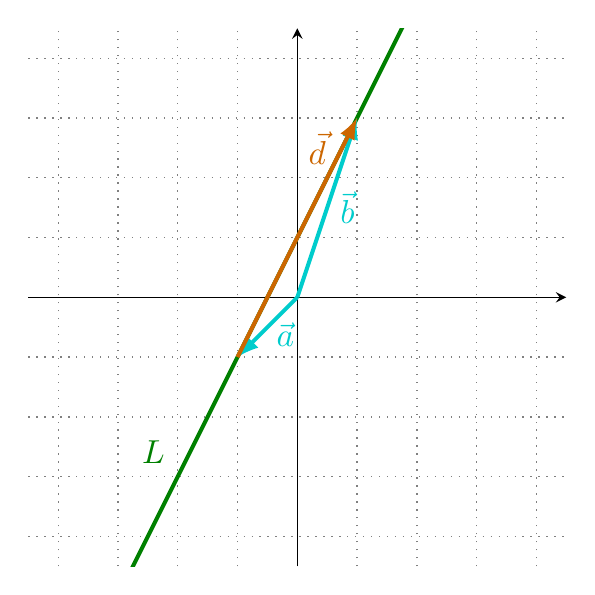
\begin{tikzpicture}[scale=1.2, >=latex]
			    \begin{axis}[scale=1,
					    axis equal image,
					    axis lines=middle,
					    axis line style = {black},
					    tick style={draw=none},
					    yticklabels={,,},
					    xticklabels={,,},
					 xmin=-4.5,
					 xmax=4.5,
					 ymin=-4.5,
					 ymax=4.5,
					 major grid style={dotted, gray},
					 xtick={-10,-9,...,10},
					 ytick={-10,-9,...,10},
					 grid=both,
					 anchor=origin]

				    \draw[Green, very thick] (-5,-9) -- (5,11) node[pos=.3, above left] {$L$};
				    \draw[cyan!80!black, very thick, ->] (0,0) -- (-1,-1) node[pos=.2, below] {$\vec a$};
				    \draw[cyan!80!black, very thick, ->] (0,0) -- (1,3) node[pos=.5, right] {$\vec b$};
				    \draw[orange!80!black, very thick, ->] (-1,-1) -- (1,3) node[near end, above, xshift=-3pt] {$\vec d$};

			    \end{axis}
				\end{tikzpicture}
			\end{solution}
		\item Is $\vec d\in L$? Explain.
			\begin{solution}
				No. $\vec d=\mat{2\\4}$ and so its entries don't satisfy $y=2x+1$.
			\end{solution}
		\item For which $t\in\R$ is it true that $\vec a+t\vec d\in L$? Explain using your picture.
			\begin{solution}
				$\vec a +t\vec d\in L$ for any $t\in \R$. We can see this because if we start at the
				vector $\vec a$ and the displace by $t\vec d$, we will always be on the line $L$.
			\end{solution}
	\end{parts}
	\begin{bookonly}\singlegrid\end{bookonly}

\begin{lesson}
	\Title{Vector Form of Lines, Intersecting Lines}

	\Heading{Textbook}
	Module 2

	\Heading{Objectives}
	\begin{itemize}
		\item Fluency with vector form of a line in $\R^2$ and $\R^3$.
		\item Recognize that vector form of a line is not unique.
		\item Find the intersection of two lines in vector form.
	\end{itemize}

	\Heading{Motivation}
	A single linear equation cannot describe a line in more than two dimensions.
	One way to describe a line that works in all dimensions is vector form, which
	is a shorthand for a particular set. Vector form has the upside that it makes it easy
	to produce points on a line, but it has the downside that it is not unique.

	\begin{annotation}
		\begin{notes}
			Giving a proper definition of vector form of a line is awkward and
			shouldn't be the focus. For vector form, that they ``know it when they see it''
			and can ``produce it'' is good enough. (This is in contrast to other definitions
			which they must be able to correctly state).
		\end{notes}
	\end{annotation}
	Vector form works because a line in any dimension can be defined by two
	points or, equivalently, a point and a direction. Though we don't yet have
	a systematic way to write solutions to a system of linear equations,
	if we have a system representing a line, all we need to do is guess two
	solutions to that system to find vector form of the line.


	\begin{annotation}
		\begin{notes}
			The biggest stumbling block for finding the intersection of two lines
			in vector form will be choosing different dummy variables before
			setting the lines equal.
		\end{notes}
	\end{annotation}
	One thing vector form makes difficult is finding intersections, but intersections
	can be turned into just another algebra problem involving a system of equations.

\end{lesson}

	\bookonlynewpage
	\SavedDefinitionRender{VectorFormofaLine}

	\question
	\begin{annotation}
		\begin{goals}
			\Goal{Practice with vector form.}

			The goal of this problem is to
			\begin{itemize}
				\item Express lines in $\R^2$ and $\R^3$ in
					vector form.
				\item Produce direction vectors by subtracting two points
					on a line.
				\item Recognize vector form is not unique.
			\end{itemize}
		\end{goals}

		\begin{notes}
			\begin{itemize}
				\item If students get stuck on part 1, ask them
					to find a vector parallel to $\ell$. If
					they're still stuck, ask them to find a vector
					connecting two points on $\ell$.
				\item Many students will intuit part 1 but get stuck on
					part 2 because they can't draw it. Ask them
					to start by finding some points on $L$.
			\end{itemize}
		\end{notes}
	\end{annotation}
	Let $\ell\subseteq \R^2$ be the line with equation $2x+y=3$,
	and let $L\subseteq \R^3$ be the line with equations $2x+y=3$ and
	$z=y$.
	\begin{parts}
		\item Write $\ell$ in vector form. Is vector form of $\ell$ unique?
			\begin{solution}
				$\vec x = t \mat{1 \\ -2} + \mat{0 \\ 3}$

				The vector form is not unique, as any non-zero scalar multiple of
				$\mat{1 \\ -2}$ can serve as a direction vector. Additionally,
				any other point on the line can be used in place of
				$\mat{0 \\3}$. For example,  $\vec x = t \mat{-4 \\ 8} + \mat{1 \\ 1}$
				is another vector form of $\ell$.
			\end{solution}
		\item Write $L$ in vector form.
			\begin{solution}[inline]
				$\vec x = t\mat{1 \\ -2 \\ -2} + \mat{0 \\ 3 \\ 3}$. This is obtained
				by finding two points: one when $x=0$ and one when $x=1$ and subtracting
				them to find a direction vector for $L$.
			\end{solution}
		\item Find another vector form for $L$ where both ``$\vec d$'' and
			``$\vec p$'' are different from before.
			\begin{solution}
				$\vec x = t \mat{-3 \\ 6 \\ 6} + \mat{1 \\ 1 \\ 1}$.

				Again, any non-zero scalar multiple of the direction vector
				will work for $\vec d$, as will any other point on the line
				work for $\vec p$.
			\end{solution}
	\end{parts}

	\bookonlynewpage
	\question
	\begin{annotation}
		\begin{goals}
			\Goal{Intersect lines in vector form.}

			The goal of this problem is to
			\begin{itemize}
				\item Practice computing the intersection between lines
					in vector form.
				\item Recognize ``$t$'' as a dummy variable as used
					in vector form and that, when comparing lines in
					vector form, ``$t$'' needs to be replaced with
					non-dummy variables.
			\end{itemize}
		\end{goals}

		\begin{notes}
			\begin{itemize}
				\item The most common mistake is to set two lines
					in vector form equal and use ``$t$'' as
					the variable in each one. Make sure to have a discussion
					about this.
			\end{itemize}
		\end{notes}
	\end{annotation}
	Let $A$, $B$, and $C$ be given in vector form by
	\[
	\overbrace{\vec x=t\mat{1\\2\\3}+\mat{0\\0\\1}}^{\displaystyle A}
	\qquad \overbrace{\vec x=t\mat{-1\\1\\1}+\mat{-1\\1\\2}}^{\displaystyle B}
	\qquad \overbrace{\vec x=t\mat{2\\-1\\1}+\mat{1\\1\\1}}^{\displaystyle C}.
	\]
	\begin{parts}
		\item Do the lines $A$ and $B$ intersect? Justify your conclusion.
			\begin{solution}
				Yes. $(0)\mat{1\\2\\3}+\mat{0\\0\\1} = \mat{0\\0\\1} = (-1)\mat{-1\\1\\1}+\mat{-1\\1\\2}$.

				To find the intersection, if there is one, we must solve the vector equation:
				\[
					t\mat{1\\2\\3}+\mat{0\\0\\1} = s\mat{-1\\1\\1}+\mat{-1\\1\\2}.
				\]
				One solution is when $t = 0$ and $s = -1$.
			\end{solution}
		\item Do the lines $A$ and $C$ intersect? Justify your conclusion.
			\begin{solution}
				No. The vector equation
				\[
					t\mat{1\\2\\3}+\mat{0\\0\\1} = s\mat{2\\-1\\1}+\mat{1\\1\\1}
				\]
				has no solutions. This is equivalent to saying that the following
				system of equations has no solutions:
				\begin{gather*}
					t = 2s + 1 \\
					2t = -s + 1 \\
					3t + 1 = s + 1
				\end{gather*}
				The third equation tells us that $s = 3t$, which when substituted
				into the first equation forces $t = -\tfrac{1}{5}$ and therefore
				$s = -\tfrac{3}{5}$. However, these two numbers don't satisfy the second
				equation.
			\end{solution}
		\item Let $\vec p\neq \vec q$ and suppose
			$X$ has vector form $\vec x=t\vec d+\vec p$ and $Y$ has
			vector form $\vec x=t\vec d+\vec q$. Is it possible
			that $X$ and $Y$ intersect?
			\begin{solution}
				Yes. If $\vec q=\vec p+a\vec d$ for $a\neq 0$, then $X$ and $Y$
				will actually be the same line, since in this case
				\[
					\vec x = t\vec d+\vec q
					= t\vec d+(\vec p+a\vec d)
					= (t+a)\vec d+\vec p.
				\]

				For example, the following two vector equations represent the
				same line.
				\[
					\vec x = t \mat{1\\1\\1} + \mat{0\\0\\0}
					\qquad \text{and} \qquad
					\vec x = t \mat{1\\1\\1} + \mat{7\\7\\7}.
				\]
			\end{solution}
	\end{parts}


\begin{lesson}
	\Title{Planes, Span}

	\Heading{Textbook}
	Module 2

	\Heading{Objectives}
	\begin{itemize}
		\item Describe a plane in vector form.
		\item Visualize spans.
		\item Recognize the dimension of $\Span(X)$ is not necessarily how many vectors
			are in $X$.
		\item Define \emph{span}.
	\end{itemize}

	\Heading{Motivation}
	Planes are just like lines but one dimension higher. Vector form of a plane is just like
	vector form of a line with all the advantages and disadvantages. But, we now have
	\emph{two} direction vectors.

	Spans are similar to lines and planes; $\Span\{\vec a,\vec b\}$ looks a lot like
	vector form of the plane
	$\vec x=t\vec a+s\vec b$. Except, $\Span\{\vec a,\vec b\}$ may not always be a plane.
	We haven't defined linear independence and linear dependence yet, but we will continue to
	foreshadow it by seeing that the dimension of the span of a set is not always the size of
	that set.

	Knowing definitions is an essential part of solving math problems. Span is
	the first definition that students will think they ``know'' but won't be
	able to write down.

\end{lesson}

	\displayonlynewpage
	\bookonlynewpage
	\SavedDefinitionRender{VectorFormofaPlane}

	\question
	\begin{annotation}
		\begin{goals}
			\Goal{Apply vector form of a plane.}

			The goal of this problem is to
			\begin{itemize}
				\item Use direction vectors for lines given in vector form.
				\item Think about planes in terms of vectors rather
					than equations.
				\item Combine direction vectors in a plane to produce new direction vectors.
			\end{itemize}
		\end{goals}

		\begin{notes}
			\begin{itemize}
				\item Students may think they need to find the intersection
					of the lines to serve as their ``$\vec p$''.
					They don't. All they need is a point
					on the plane!
			\end{itemize}
		\end{notes}
	\end{annotation}
	Recall the intersecting lines $A$ and $B$ given in vector form by
	\[
		\overbrace{\vec x=t\mat{1\\2\\3}+\mat{0\\0\\1}}^{\displaystyle A}
		\qquad
		\overbrace{\vec x=t\mat{-1\\1\\1}+\mat{-1\\1\\2}}^{\displaystyle B}.
	\]
	Let $\mathcal P$ the plane that contains the lines $A$ and $B$.
	\begin{parts}
		\item Find two direction vectors for $\mathcal P$.
			\begin{solution}
				Two possible answers are:
				\[
					\vec d_1 = \mat{1\\2\\3}
					\qquad \text{and} \qquad
					\vec d_2 = \mat{-1\\1\\1}.
				\]
				These are the two direction vectors we already know are in the
				plane---the ones from the two lines:

				Note that neither of these is a multiple of the other, so they
				really are two unique direction vectors in $\mathcal P$.
			\end{solution}
		\item Write $\mathcal P$ in vector form.
			\begin{solution}
				\[
					\vec x = t\vec d_1 +s\vec d_2+\vec p
					= t \mat{1\\2\\3} + s \mat{-1\\1\\1} + \mat{0\\0\\1}.
				\]
				We already have two direction vectors, so we just needed a point
				on the plane. We used the point $\vec p = \mat{0\\0\\1}$
				that we already know is on line $A$.
			\end{solution}
		\item Describe how vector form of a plane relates to linear
			combinations.
			\begin{solution}
				The vector form of a plane says that a vector $\vec x$ is on the
				plane exactly when it is equal to some linear combination of
				$\vec d_1$ and $\vec d_2$, plus $\vec p$.

				Another way of saying
				the same thing is that the vector $\vec x$ is on the plane
				exactly when $\vec x - \vec p$ is equal	to some linear
				combination of $\vec d_1$ and $\vec d_2$.
			\end{solution}
		\item Write $\mathcal P$ in vector form using different
			direction vectors and a different point.
			\begin{solution}
				One possible answer:
				\[
					\vec x = t\mat{-1\\-2\\-3}+s\mat{-7\\7\\7}+\mat{-1\\1\\2}.
				\]
				As with the equations of lines from before, we can use any
				non-zero scalar multiple of either direction vector and get the
				same plane. We also used the point $\vec q = \mat{-1\\1\\2}$
				that we already knew is on line $B$.
			\end{solution}
	\end{parts}

	\bookonlynewpage
	\question
	\label{ProbPlane}
	\begin{annotation}
		\begin{goals}
			\Goal{Connect vector form and scalar form of a plane.}

			The goal of this problem is to
			\begin{itemize}
				\item Produce direction vectors for a plane defined by
					an equation.
				\item Generalize the procedure for finding direction
					vectors that was used for lines.
			\end{itemize}
		\end{goals}

		\begin{notes}
			\begin{itemize}
				\item This problem is scaffolded and should be straight forward.
				\item You have the opportunity to discuss if $\vec x=t\vec d+s(-\vec d)+\vec p$
					is a valid vector form of $\mathcal P$. The two direction vectors
					are different, after all.
			\end{itemize}
		\end{notes}
	\end{annotation}
	Let $\mathcal Q\subseteq \R^3$ be a plane with equation $x+y+z=1$.
	\begin{parts}
		\item Find three points in $\mathcal Q$.
			\begin{solution}
				There are many choices here, of course. Three natural ones are:
				\[
					\vec p_1 = \mat{1\\0\\0}
					\qquad
					\vec p_2 = \mat{0\\1\\0}
					\qquad
					\vec p_3 = \mat{0\\0\\1}
				\]
			\end{solution}
		\item Find two direction vectors for $\mathcal Q$.
			\begin{solution}
				Now that we have three points on the plane, we can use the
				direction vectors joining any two pairs of them. For example:
				\[
					\vec d_1 = \vec p_1 - \vec p_2 = \mat{1\\-1\\0}
					\qquad
					\vec d_2 = \vec p_1 - \vec p_3 = \mat{1\\0\\-1}.
				\]
			\end{solution}
		\item Write $\mathcal Q$ in vector form.
			\begin{solution}
				Using the point $\vec p_1$ from above, one possible answer is:
				\[
					\vec x = t\vec d_1 + s\vec d_2 + \vec p_1
					= t \mat{1\\-1\\0} + s \mat{1\\0\\-1} + \mat{1\\0\\0}.
				\]
			\end{solution}
	\end{parts}

\begin{module}
	\Title{Spans, Translated Spans, and Linear Independence/Dependence}

	In this module you will learn
	\begin{itemize}
		\item The definition of span and how to visualize spans.
		\item How to express lines/planes/volumes through the origin as spans.
		\item How to express lines/planes/volumes \emph{not} through the origin as
			\emph{translated} spans using set addition.
		\item Geometric and algebraic definitions of linear independence and linear
			dependence.
		\item How to find linearly independent subsets.
	\end{itemize}

	Let $\vec u=\mat{1\\1}$ and $\vec v=\mat{1\\-2}$. Can the vectors $\vec w=\mat{2\\5}$ be obtained
as a linear combination of $\vec u$ and $\vec v$?

By drawing a picture, the answer appears to be \emph{yes}.

\begin{center}
	\begin{tikzpicture}
		\begin{axis}[
		    anchor=origin,
		    disabledatascaling,
		    xmin=-1,xmax=3,
		    ymin=-2,ymax=5,
			xtick={-2,...,3},
		    x=1cm,y=1cm,
		    grid=both,
		    grid style={line width=.1pt, draw=gray!10},
		    %major grid style={line width=.2pt,draw=gray!50},
		    axis lines=middle,
		    minor tick num=0,
		    enlargelimits={abs=0.5},
		    axis line style={latex-latex},
		    ticklabel style={font=\tiny,fill=white},
		    xlabel style={at={(ticklabel* cs:1)},anchor=north west},
		    ylabel style={at={(ticklabel* cs:1)},anchor=south west}
		]

			\draw [myorange, thick, ->] (0,0) -- (1,1) node[midway, below] {$\vec u$};
			\draw [mypink, thick, ->] (0,0) -- (1,-2) node[midway, below left] {$\vec v$};
			\draw [mygreen, thick, dashed, ->] (0,0) -- (2,5) node[midway, above left] {$\vec w$};
			%\draw [black!70!white, thick,dashed, ->, xshift=-.15cm] (0,0) -- (0,1) node[midway, left] {$\yhat$};
		\end{axis}
	\end{tikzpicture}
	~~~~
	\begin{tikzpicture}
		\begin{axis}[
		    anchor=origin,
		    disabledatascaling,
		    xmin=-1,xmax=3,
		    ymin=-2,ymax=5,
			xtick={-2,...,3},
		    x=1cm,y=1cm,
		    grid=both,
		    grid style={line width=.1pt, draw=gray!10},
		    %major grid style={line width=.2pt,draw=gray!50},
		    axis lines=middle,
		    minor tick num=0,
		    enlargelimits={abs=0.5},
		    axis line style={latex-latex},
		    ticklabel style={font=\tiny,fill=white},
		    xlabel style={at={(ticklabel* cs:1)},anchor=north west},
		    ylabel style={at={(ticklabel* cs:1)},anchor=south west}
		]

			\draw [black!70!white, thick, ->] (0,0) -- (1,1);
			\draw [black!70!white, thick, ->] (1,1) -- (2,2) node[midway, below right] {$3\vec u$};
			\draw [black!70!white, thick, ->] (2,2) -- (3,3);
			\draw [black!70!white, thick, ->] (3,3) -- (2,5) node[midway, below left] {$-\vec v$};
			\draw [mygreen, thick, dashed, ->] (0,0) -- (2,5) node[midway, above left] {$\vec w$};
			%\draw [black!70!white, thick,dashed, ->, xshift=-.15cm] (0,0) -- (0,1) node[midway, left] {$\yhat$};
		\end{axis}
	\end{tikzpicture}
\end{center}

Algebraically, we can use the definition of a \emph{linear combination} to set up a system of equations.
We know $\vec w$ can be expressed as a linear combination of $\vec u$ and $\vec v$ if and only if 
the vector equation
\[
	\vec w = \mat{2\\5}=\alpha\mat{1\\1}+\beta\mat{1\\-2}=\alpha \vec u+\beta \vec v
\]
has a solution. By inspection, we see $\alpha=3$ and $\beta=-1$ solve this equation.

After initial success, we might ask the following:
\emph{what are all the locations in $\R^2$ that can be obtained
as a linear combination of $\vec u$ and $\vec v$?} Geometrically, it appears
any location can be reached. To verify this algebraically, consider the vector equation
\begin{equation}
	\label{EQSPAN1}
	\vec x=\mat{x\\y} = \alpha\mat{1\\1}+\beta\mat{1\\-2} = \alpha\vec u+\beta\vec v.
\end{equation}
Here $\vec x$ represents an arbitrary point in $\R^2$. If equation \eqref{EQSPAN1} always
has a solution\footnote{ The official terminology would be to say that
the equations are always \emph{consistent}.}, any vector in $\R^2$ can be obtained as a linear combination of $\vec u$ and $\vec v$.

We can solve this equation for $\alpha$ and $\beta$ by considering the equations arising from the
first and second coordinates. Namely,
	\[
		\sysdelim..\systeme*{x=\alpha+\beta, y=\alpha-2\beta}
	\]
Subtracting the second equation from the first, we get $x-y=3\beta$ and so $\beta=(x-y)/3$. Plugging 
$\beta$ into the first equation and solving, we get $\alpha=(2x+y)/3$. Thus, equation \eqref{EQSPAN1}
\emph{always} has the solution
\begin{align*}
	\alpha &= \tfrac{1}{3}(2x+y)\\
	\beta &= \tfrac{1}{3}(x-y).
\end{align*}

There is a formal term for the set of vectors that can be obtained as linear combinations
of others: \emph{span}\index{Span}.

\SavedDefinitionRender{Span}

We just showed above that $\Span\Set*{\mat{1\\1},\mat{1\\-2}}=\R^2$.

\begin{example}
	Let $\vec u=\mat{-1\\2}$ and $\vec v=\mat{1\\-2}$. Find $\Span\Set{\vec u,\vec v}$.

	By the definition of span,
	\[
		\Span\Set{\vec u,\vec v}=
		\Set{\vec x\given \vec x=\alpha\vec u+\beta\vec v\text{ for some }\alpha,\beta\in\R}.
	\]
	We need to determine for which $x$ and $y$ the vector equation $\mat{x\\y} = \alpha\mat{-1\\2}+\beta\mat{1\\-2}$ is consistent.
	
	From the first and second coordinates, we get the system
	\[
		\sysdelim..\systeme*{x=-\alpha+\beta, y=2\alpha-2\beta}.
	\]
	Adding 2 times the first equation to the second, we get $2x+y=0$ and so $y=-2x$.
	Therefore, if $\mat{x\\y}$ makes the above system consistent, we must have
	\[
		\mat{x\\y}=\mat{t\\-2t}=t\vec v
	\]
	for some $t$.
	Thus,
	\[
		\Span\Set{\vec u,\vec v}=
		\Set{\vec x\given \vec x=t\vec v\text{ for some }t}=\Span\Set{\vec v},
	\]
	which is a line through the origin with direction $\vec v$.
\end{example}

\begin{example}
	Let $\vec a=\mat{1\\2\\1}$, $\vec b=\mat{0\\1\\0}$, and $\vec c=\mat{1\\1\\2}$. Show that
	$\R^3=\Span\Set{\vec a,\vec b,\vec c}$.

	If the equation 
	\[
		\vec x=\mat{x\\y\\z} = \alpha_1\mat{1\\2\\1}+\alpha_2\mat{0\\1\\0}+\alpha_3\mat{1\\1\\2}
		 = \alpha_1\vec a+\alpha_2\vec b+\alpha_3\vec c
	\]
	is always consistent, then any vector in $\R^3$ can be obtained as a linear combination of
	$\vec a, \vec b$, and $\vec c$.
	
	Reading off the coordinates, we get the system
	\[
		\sysdelim..\systeme*{x=\alpha_1+\alpha_3, y=2\alpha_1+\alpha_2+\alpha_3, z=\alpha_1+2\alpha_3}.
	\]
	Solving this system, we see
	\[
		\begin{aligned}
			\alpha_1&=2x-z\\
			\alpha_2&=-3x+y+z\\
			\alpha_3&=-x+z
		\end{aligned}
	\]
	is always a solution (no matter the values of $x$, $y$, and $z$). Therefore,
	$\Span\Set{\vec a,\vec b,\vec c}=\R^3$.
\end{example}

\Heading{Representing Lines \& Planes as Spans}

If spans remind you of vector forms of lines and planes, your intuition is keen.
Consider the line $\ell$ given in vector form by
\[
	\vec x=t\vec d+\vec 0.
\]
The line $\ell$ passes through the origin, and if we unravel its definition, we see
\[
	\ell=\Set{\vec x\given \vec x=t\vec d+\vec 0\text{ for some }t\in \R}
	=\Set{\vec x\given \vec x=t\vec d\text{ for some }t\in \R}=\Span\Set{\vec d}.
\]

Similarly, if $\mathcal P$ is a plane given in vector form by
\[
	\vec x=t\vec d_1+s\vec d_2+\vec 0,
\]
then
\[
	\mathcal P=
	\Set{\vec x\given \vec x=t\vec d_1+s\vec d_2\text{ for some }t,s\in \R}=\Span\Set{\vec d_1,\vec d_2}.
\]

If the ``$\vec p$'' in our vector form is $\vec 0$, then that vector form actually defines
a span. This means (if you accept that every line/plane through the origin has a
vector form) that every line/plane through the origin can be written as a span. Conversely,
if $X=\Span\Set{\vec v_1,\ldots,\vec v_n}$ is a span, we know $\vec 0=0\vec v_1+\cdots+0\vec v_n\in X$,
and so every span passes through the origin.


As it turns out, spans exactly describe points, lines, planes, and volumes\index{Volume}\footnote{
 We use the word \emph{volume} to indicate the higher-dimensional analogue of a plane.} through the origin.

\begin{example}
	The line $\ell_1\subseteq\R^2$ is described by the equation $x+2y=0$ and the line 
	$\ell_2\subseteq \R^2$ is described by the equation $4x-2y=6$.
	If possible, describe $\ell_1$ and $\ell_2$ using spans.

	We can express $\ell_1$ in vector form by
	\[
		\vec x=t\mat{2\\-1}+\vec 0,
	\]
	and so 
	\[
		\ell_1=\Span\Set*{\mat{2\\-1}}.
	\]

	However, $\ell_2$ does not pass through $\vec 0$, and so $\ell_2$ cannot be written as a span.
\end{example}

\begin{emphbox}[Takeaway]
	Lines and planes through the origin, and only lines and planes through the origin, can be expressed as spans.
\end{emphbox}

\Heading{Set Addition}
We're going to work around the fact that only objects which pass through the origin can be written as
spans, but first let's take a detour and learn about \emph{set addition}.

\SavedDefinitionRender{SetAddition}

Set sums are very different than regular sums despite using the same symbol, ``$+$''\footnote{
For example, $A+\Set{}=\Set{}$, which might seem counterintuitive for an ``addition'' operation.
}.
 However, they are very useful.
Let $C=\Set{\vec x\in\R^2\given \norm{\vec x}=1}$ be the unit circle centered at the origin, and consider
the sets
\[
	X=C+\Set{\yhat}\qquad Y=C+\Set{3\xhat,\yhat}\qquad Z=C+\Set{\vec 0, \xhat,\yhat}.
\]
Rewriting, we see $X=\Set{\vec x+\yhat\given \norm{\vec x}=1}$ is just $C$ translated
by $\yhat$. Similarly, $Y=\Set{\vec x+\vec v\given \norm{\vec x}=1\text{ and }\vec v=3\xhat\text{
	or }\vec v=\yhat}=(C+\Set{3\xhat})\cup (C+\Set{\yhat})$, and so $Y$ is the union
of two translated copies of $C$\footnote{ If you want to stretch your mind, consider what $C+C$
is as a set.}. Finally, $Z$ is the union of three translated copies of $C$.

\begin{center}
	\begin{tikzpicture}
		\begin{axis}[
		    anchor=origin,
		    disabledatascaling,
		    xmin=-1,xmax=1,
		    ymin=-1,ymax=2,
			xtick={-2,...,4},
		    x=1cm,y=1cm,
		    grid=both,
		    grid style={line width=.1pt, draw=gray!10},
		    %major grid style={line width=.2pt,draw=gray!50},
		    axis lines=middle,
		    minor tick num=0,
		    enlargelimits={abs=0.5},
		    axis line style={latex-latex},
		    ticklabel style={font=\tiny,fill=white},
		    xlabel style={at={(ticklabel* cs:1)},anchor=north west},
		    ylabel style={at={(ticklabel* cs:1)},anchor=south west}
		]

			\draw[myorange, thick] (0,1) circle (1cm) node[right] {$X$};
		\end{axis}
	\end{tikzpicture}
	~~~~
	\begin{tikzpicture}
		\begin{axis}[
		    anchor=origin,
		    disabledatascaling,
		    xmin=-1,xmax=4,
		    ymin=-1,ymax=2,
			xtick={-2,...,4},
		    x=1cm,y=1cm,
		    grid=both,
		    grid style={line width=.1pt, draw=gray!10},
		    %major grid style={line width=.2pt,draw=gray!50},
		    axis lines=middle,
		    minor tick num=0,
		    enlargelimits={abs=0.5},
		    axis line style={latex-latex},
		    ticklabel style={font=\tiny,fill=white},
		    xlabel style={at={(ticklabel* cs:1)},anchor=north west},
		    ylabel style={at={(ticklabel* cs:1)},anchor=south west}
		]

			\draw[mypink, thick] (0,1) circle (1cm) (3,0) circle (1cm) node[above right] {$Y$};
		\end{axis}
	\end{tikzpicture}
	~~~~
	\begin{tikzpicture}
		\begin{axis}[
		    anchor=origin,
		    disabledatascaling,
		    xmin=-1,xmax=2,
		    ymin=-1,ymax=2,
			xtick={-2,...,4},
		    x=1cm,y=1cm,
		    grid=both,
		    grid style={line width=.1pt, draw=gray!10},
		    %major grid style={line width=.2pt,draw=gray!50},
		    axis lines=middle,
		    minor tick num=0,
		    enlargelimits={abs=0.5},
		    axis line style={latex-latex},
		    ticklabel style={font=\tiny,fill=white},
		    xlabel style={at={(ticklabel* cs:1)},anchor=north west},
		    ylabel style={at={(ticklabel* cs:1)},anchor=south west}
		]

			\draw[mygreen, thick] (0,0) circle (1cm) (0,1) circle (1cm) (1,0) circle (1cm) node[above right] {$Z$};
		\end{axis}
	\end{tikzpicture}
\end{center}

\Heading{Translated Spans}\index{Span!translated}

Set addition allows us to easily create parallel lines and planes by translation. For example,
consider the lines $\ell_1$ and $\ell_2$ given in vector form as $\vec x=t\vec d$ and $\vec x=t\vec d+\vec p$,
respectively, where  $\vec d=\mat{2\\1}$ and $\vec p=\mat{-1\\1}$.  These lines
differ from each other by a translation. That is, every point in $\ell_2$ can be obtained by adding $\vec p$ to
a corresponding point in $\ell_1$. Using the idea of set addition, we can express this relationship
by the equation
\[
	\ell_2 = \ell_1+\Set{\vec p}.
\]

\begin{center}
	\begin{tikzpicture}
		\begin{axis}[
		    anchor=origin,
		    disabledatascaling,
		    xmin=-1,xmax=4,
		    ymin=-1,ymax=3,
			xtick={-2,...,4},
		    x=1cm,y=1cm,
		    grid=both,
		    grid style={line width=.1pt, draw=gray!10},
		    %major grid style={line width=.2pt,draw=gray!50},
		    axis lines=middle,
		    minor tick num=0,
		    enlargelimits={abs=0.5},
		    axis line style={latex-latex},
		    ticklabel style={font=\tiny,fill=white},
		    xlabel style={at={(ticklabel* cs:1)},anchor=north west},
		    ylabel style={at={(ticklabel* cs:1)},anchor=south west}
		]

			\draw[myorange,very thick] (-2,-1) -- (6,3) node[midway, below right] {$\ell_1$};
			\draw[mygreen, thick] (-3,0) -- (5,4) node[near end, above left] {$\ell_2=\ell_1+\Set{\vec p}$};
			\draw[black!50!white, thick,dotted, ->] (0,0) -- +(-1,1) node[midway, below left, yshift=2pt] {$\vec p$};
		\end{axis}
	\end{tikzpicture}
	~~~~
	\begin{tikzpicture}
		\begin{axis}[
		    anchor=origin,
		    disabledatascaling,
		    xmin=-1,xmax=4,
		    ymin=-1,ymax=3,
			xtick={-2,...,4},
		    x=1cm,y=1cm,
		    grid=both,
		    grid style={line width=.1pt, draw=gray!10},
		    %major grid style={line width=.2pt,draw=gray!50},
		    axis lines=middle,
		    minor tick num=0,
		    enlargelimits={abs=0.5},
		    axis line style={latex-latex},
		    ticklabel style={font=\tiny,fill=white},
		    xlabel style={at={(ticklabel* cs:1)},anchor=north west},
		    ylabel style={at={(ticklabel* cs:1)},anchor=south west}
		]

			\draw[myorange, very thick] (-2,-1) -- (6,3) node[pos=.15, below right] {$\ell_1$};
			\draw[black, thick, dashed, ->] (0,0) -- (3,1.5) node[midway, below right] {$\tfrac{3}{2}\vec d\in\ell_1$};
			\draw[mygreen, thick] (-3,0) -- (5,4);% node[near end, above left] {$\ell_1+\Set{\vec p}$};
			\draw[black!50!white, thick,dotted, ->] (0,0) -- +(-1,1);
			\draw[black!50!white, thick,dotted, ->] (-1,-1/2) -- +(-1,1);
			\draw[black!50!white, thick,dotted, ->] (1,1/2) -- +(-1,1);
			\draw[black!50!white, thick,dotted, ->] (2,1) -- +(-1,1);
			\fill[black!60!white] (2,2.5) circle (1.5pt);
			\draw[black, thick,dashed, ->] (3,3/2) -- +(-1,1) node[midway, above right] {$\vec p$} 
			node[above left]{$\tfrac{3}{2}\vec d+\vec p\in\ell_2$};
			\draw[black!50!white, thick,dotted, ->] (4,2) -- +(-1,1);
		\end{axis}
	\end{tikzpicture}
\end{center}

Note: it would be incorrect to write ``$\ell_2=\ell_1+\vec p$''. Because $\ell_1$
is a set and $\vec p$ is not a set, ``$\ell_1+\vec p$'' does not make mathematical sense.

\begin{example}
	Recall $\ell_2\subseteq\R^2$ is the line described by the equation $4x-2y=6$.
	Describe $\ell_2$ as a translated span.

	We can express $\ell_2$ in vector form with the equation
	\[
		\vec x=t\mat{1\\2}+\mat{1\\-1}.
	\]
	Therefore,
	\[
		\ell_2=\Span\Set*{\mat{1\\2}}+\Set*{\mat{1\\-1}}.
	\]
\end{example}

We can now see translated spans provide an alternative notation to vector form 
for specifying lines and planes. If $Q$ is described in vector form by
\[
	\vec x=t\vec d_1+s\vec d_2+\vec p,
\]
then
\[
	Q=\Span\Set{\vec d_1,\vec d_2}+\Set{\vec p}.
\]



\begin{emphbox}[Takeaway]
	All lines and planes, whether through the origin or not, can be expressed as translated
	spans.
\end{emphbox}

\Heading{Linear Independence \& Linear Dependence}

Let
\[
	\vec u=\mat{1\\0\\0}\qquad\vec v=\mat{0\\1\\0}\qquad \vec w=\mat{1\\1\\0}.
\]
Since $\vec w=\vec u+\vec v$, we know that $\vec w\in\Span\Set{\vec u,\vec v}$. Geometrically,
this is also clear because $\Span\Set{\vec u,\vec v}$ is the $xy$-plane in $\R^3$ and 
$\vec w$ lies on that plane.

What about $\Span\Set{\vec u,\vec v,\vec w}$? Intuitively, since $\vec w$ is already
a linear combination of $\vec u$ and $\vec v$, we can't get anywhere \emph{new} by
taking linear combinations of $\vec u$, $\vec v$, \emph{and} $\vec w$ compared to linear combinations
of just $\vec u$ and $\vec v$. So $\Span\Set{\vec u,\vec v}=\Span\Set{\vec u,\vec v,\vec w}$.

Can we prove this from the definitions? Yes! Suppose $\vec r\in \Span\Set{\vec u,\vec v,\vec w}$.
By definition,
\[
	\vec r=\alpha\vec u+\beta\vec v+\gamma\vec w
\] for some $\alpha,\beta,\gamma\in\R$. Since $\vec w=\vec u+\vec v$, we see
\[
	\vec r=\alpha\vec u+\beta\vec v+\gamma(\vec u+\vec v) 
	= (\alpha+\gamma)\vec u+(\beta+\gamma)\vec v\in\Span\Set{\vec u,\vec v}.
\]
Thus, $\Span\Set{\vec u,\vec v,\vec w}\subseteq \Span\Set{\vec u,\vec v}$. Conversely, if $\vec s\in\Span\Set{\vec u,\vec v}$,
by definition,
\[
	\vec s=a\vec u+b\vec v=a\vec u+b\vec v+0\vec w
\]
for some $a,b\in \R$,
and so $\vec s\in\Span\Set{\vec u,\vec v,\vec w}$. Thus $\Span\Set{\vec u,\vec v}\subseteq\Span\Set{\vec u,\vec v,\vec w}$.
We conclude $\Span\Set{\vec u,\vec v}=\Span\Set{\vec u,\vec v,\vec w}$.

In this case, $\vec w$ was a redundant vector---it wasn't needed for the span. When a set contains
a redundant vector, we call the set \emph{linearly dependent}.

\SavedDefinitionRender{LinearlyDependentIndependentGeometric}

We will also refer to sets of vectors (for example $\Set{\vec v_1,\ldots,\vec v_n}$) as being linearly
independent or linearly dependent. For technical reasons, we didn't state the definition in terms
of sets\footnote{ The issue is, every element of a set is unique. Clearly, the vectors $\vec v$ and $\vec v$
are linearly dependent, but $\Set{\vec v,\vec v}=\Set{\vec v}$, and so $\Set{\vec v,\vec v}$ is technically
a linearly independent set. This issue would be resolved by talking about \emph{multisets} instead of sets,
but it isn't worth the hassle.}.

The geometric definition of linear dependence says that the vectors $\vec v_1,\ldots,\vec v_n$ are linearly dependent
if you can remove at least one vector without changing the span. In other words, $\vec v_1,\ldots,\vec v_n$ 
are linearly dependent \emph{if there is a redundant vector}.

\begin{example}
	\label{EXLINDEP}
	Let $\vec a=\mat{1\\2}$, $\vec b=\mat{2\\3}$, $\vec c=\mat{4\\6}$, and $\vec d=\mat{4\\5}$. Determine whether
	$\Set{\vec a,\vec b,\vec c,\vec d}$ is linearly independent or linearly dependent.

	By inspection, we see $\vec c=2\vec b$. Therefore,
	\[
		\Span\Set{\vec a,\vec b,\vec c,\vec d}=\Span\Set{\vec a,\vec b,\vec d},
	\]
	and so $\Set{\vec a,\vec b,\vec c,\vec d}$ is linearly dependent.
\end{example}

\begin{example}
	The planes $\mathcal P$ and $\mathcal Q$ are given in vector form by
	\[
		\overbrace{\vec x=t\mat{1\\2\\1}+s\mat{2\\2\\1}}^{\mathcal P}
		\qquad\text{and}\qquad
		\overbrace{\vec x=t\mat{3\\4\\2}+s\mat{2\\2\\1}}^{\mathcal Q}.
	\]
	Determine if $\mathcal P$ and $\mathcal Q$ are the same plane.

	Let $\vec a_1=\mat{1\\2\\1}$ and $\vec a_2=\mat{2\\2\\1}$ be the direction vectors
	for $\mathcal P$ and let
	$\vec b_1=\mat{3\\4\\2}$ and $\vec b_2=\mat{2\\2\\1}$ be the direction vectors
	for $\mathcal Q$. We know that $\mathcal P=\mathcal Q$ if every direction vector for $\mathcal Q$
	is a linear combination of the direction vectors for $\mathcal P$. In other words, 
	$\mathcal P=\mathcal Q$ if
	\[
		\Set{\vec a_1,\vec a_2,\vec b_1}\qquad\text{and}\qquad \Set{\vec a_1,\vec a_2,\vec b_2}
	\]
	are both linearly dependent sets. Since $\vec a_2=\vec b_2$, clearly $\Set{\vec a_1,\vec a_2,\vec b_2}$
	is linearly dependent. 

	We will now check whether $\Set{\vec a_1,\vec a_2,\vec b_1}$ is linearly dependent. Since $\Set{\vec a_1,\vec a_2}$
	is a linearly independent set, we only need to check if $\vec b_1$ can be written as a linear combination of $\vec a_1$ and $\vec a_2$.
	After solving the system
	\[
		\mat{3\\4\\2}=x\mat{1\\2\\1}+y\mat{2\\2\\1},
	\]
	we see that $\vec b_1=\vec a_1+\vec a_2$, and so $\Set{\vec a_1,\vec a_2,\vec b_1}$ is linearly dependent. Therefore,
	$\mathcal P=\mathcal Q$.
\end{example}

We can also think of linear independence/dependence from an algebraic perspective.
Suppose the vectors $\vec u$, $\vec v$, and $\vec w$ satisfy 
\begin{equation}
	\label{EQLIND}
	\vec w=\vec u+\vec v.
\end{equation}
The set
$\Set{\vec u,\vec v,\vec w}$ is linearly dependent since $\vec w\in\Span\Set{\vec u,\vec v}$,
but equation \eqref{EQLIND} can be rearranged
to get
\begin{equation}
	\label{EQLIND2}
	\vec 0=\vec u+\vec v-\vec w.
\end{equation}
Here we have expressed $\vec 0$ as a linear combination of $\vec u$, $\vec v$, and $\vec w$.
By itself, this is nothing special. After all, we know $\vec 0=0\vec u+0\vec v+0\vec w$
is a linear combination of $\vec u$, $\vec v$, and $\vec w$. However, the right side of equation \eqref{EQLIND2} has non-zero
coefficients, which makes the linear combination \emph{non-trivial}.

\SavedDefinitionRender{TrivialLinearCombination}

We can always write $\vec 0$ as a linear combination of vectors if we let all the coefficients
be zero, but it turns out we can only write $\vec 0$ as a \emph{non-trivial} linear combination
of vectors if those vectors are linearly dependent. This is the inspiration for another definition
of linear independence/dependence.

\SavedDefinitionRender{LinearlyDependentIndependentAlgebraic}

The idea of a ``redundant vector'' coming from the geometric definition of linear dependence
is easy to visualize, but it can be hard to prove things with---checking for linear independence
with the geometric definition involves verifying for every vector that it is not in the span of the others.
The algebraic definition on the other hand is less obvious, but the reasoning is easier.
You only need to analyze solutions to one equation!

\begin{example}
	Let $\vec u=\mat{1\\2}$, $\vec v=\mat{2\\3}$, and $\vec w=\mat{4\\5}$. Use the algebraic definition
	of linear independence to determine whether
	$\Set{\vec u,\vec v,\vec w}$ is linearly independent or dependent.

	We need to determine if there is a non-trivial solution to 
	\[
		x\vec u+y\vec v+z\vec w=\vec 0.
	\]
	This vector equation is equivalent to the system of equations
	\[
		\systeme{x+2y+4z=0,2x+3y+5z=0}.
	\]
	Solving this system using row reduction, we see the complete solution set can be expressed as
	\[
		\mat{x\\y\\z}=t\mat{2\\-3\\1}.
	\]
	In particular, $(x,y,z)=(2,-3,1)$ is a non-trivial solution to this system. Therefore $\Set{\vec u,\vec v,\vec w}$
	is linearly dependent.
\end{example}


\begin{theorem}
	The geometric and algebraic definitions of linear independence are equivalent.
\end{theorem}
\begin{proof}
	To show the two definitions are equivalent, we need to show that geometric~$\implies$~algebraic
	and algebraic~$\implies$~geometric.

	\medskip
	\noindent
	(geometric~$\implies$~algebraic) Suppose $\vec v_1,\ldots,\vec v_n$ are linearly dependent by the 
	geometric definition. That means that for some $i$, we have
	\[
		\vec v_i \in \Span\Set{\vec v_1,\ldots,\vec v_{i-1},\vec v_{i+1},\ldots,\vec v_n}.
	\]
	Fix such an $i$. Then, by the definition of span we know
	\[
		\vec v_i=\alpha_1\vec v_1+\cdots \alpha_{i-1}\vec v_{i-1}+\alpha_{i+1}\vec v_{i+1}+\cdots +\alpha_n\vec v_n,
	\]
	and so
	\[
		\vec 0=\alpha_1\vec v_1+\cdots \alpha_{i-1}\vec v_{i-1}-\vec v_i+\alpha_{i+1}\vec v_{i+1}+\cdots +\alpha_n\vec v_n.
	\]
	This must be a non-trivial linear combination because the coefficient of $\vec v_i$ is $-1\neq 0$. Therefore, 
	$\vec v_1,\ldots,\vec v_n$ is linearly dependent by the algebraic definition.
	
	\medskip
	\noindent
	(algebraic~$\implies$~geometric) Suppose $\vec v_1,\ldots,\vec v_n$ are linearly dependent by the 
	algebraic definition. That means there exist $\alpha_1,\ldots,\alpha_n$, not all zero, so that
	\[
		\vec 0=\alpha_1\vec v_1+\cdots +\alpha_n\vec v_n.
	\]
	Fix $i$ so that $\alpha_i\neq 0$ (why do we know there is such an $i$?). Rearranging we get
	\[
		-\alpha_i\vec v_i=\alpha_1\vec v_1+\cdots \alpha_{i-1}\vec v_{i-1}+\alpha_{i+1}\vec v_{i+1}+\cdots +\alpha_n\vec v_n,
	\]
	and since $\alpha_i\neq 0$, we can multiply both sides by $\frac{-1}{\alpha_i}$ to get
	\[
		\vec v_i=\tfrac{-\alpha_1}{\alpha_i}\vec v_1+\cdots +\tfrac{-\alpha_{i-1}}{\alpha_i}\vec v_{i-1}
	+\tfrac{-\alpha_{i+1}}{\alpha_i}\vec v_{i+1}+\cdots +\tfrac{-\alpha_n}{\alpha_i}\vec v_n.
	\]
	This shows that
	\[
		\vec v_i \in \Span\Set{\vec v_1,\ldots,\vec v_{i-1},\vec v_{i+1},\ldots,\vec v_n},
	\]
	and so $\vec v_1,\ldots,\vec v_n$ is linearly dependent by the geometric definition.
\end{proof}

\Heading{Linear Independence and Unique Solutions}

The algebraic definition of linear independence can teach us something about
solutions to systems of equations. 

Recall the linearly dependent vectors 
\[
	\vec u=\mat{1\\0\\0}\qquad \vec v=\mat{0\\1\\0}\qquad \vec w=\mat{1\\1\\0}
\]
which satisfy the non-trivial relationship $\vec u+\vec v-\vec w=\vec 0$. Since $\vec u+\vec v-\vec w=\vec 0$
is a non-trivial relationship giving $\vec 0$, we can use it to generate others. For example,
\begin{alignat*}{2}
	17(\vec u+\vec v-\vec w)\ &=\ 17\vec u+17\vec v-17\vec w\ &=\ 17\vec 0\ &=\ \vec 0\\
	-3(\vec u+\vec v-\vec w)\ &=\ -3\vec u-3\vec v+3\vec w\ &=\ -3\vec 0\ &=\ \vec 0\\
	&\hspace{5em}\vdots&&
\end{alignat*}
are all different non-trivial linear combinations that give $\vec 0$. In other words, if 
the equation $\alpha\vec u+\beta \vec v+\gamma \vec w=\vec 0$ has a non-trivial solution,
it has \emph{infinitely many} non-trivial solutions. Conversely, if  the equation
$\alpha\vec u+\beta \vec v+\gamma \vec w=\vec 0$ has infinitely many solutions, one of them
has to be non-trivial!

Equations where one side is $\vec 0$ show up often and are called \emph{homogeneous} equations.
\SavedDefinitionRender{HomogeneousSystem}

This insight links linear independence and homogeneous systems together, and is encapsulated
in the following theorem.

\begin{theorem}
	The vectors $\vec v_1$, \ldots, $\vec v_n$ are linearly independent if and only if
	the homogeneous equation
	\[
		\alpha_1\vec v_1+\cdots +\alpha_n\vec v_n=\vec 0
	\]
	has a unique solution.
\end{theorem}

This theorem has a practical application: suppose you wanted to decide if the vectors $\vec a$, $\vec b$, and
$\vec c$ were linearly dependent. You could (i) find a non-trivial solution to $x\vec a+y\vec b+z\vec c=\vec 0$, 
or (ii) merely show that $x\vec a+y\vec b+z\vec c=\vec 0$ has more than one solution. Sometimes one is easier than
the other.

\Heading{Linear Independence and Vector Form}

The equation
\[
	\vec x=t_1\vec d_1+t_2\vec d_2
\]
represents a plane in vector form whenever $\vec d_1$ and $\vec d_2$ are non-zero, non-parallel vectors.
In other words, 
	$\vec x=t_1\vec d_1+t_2\vec d_2$
	represents a plane whenever $\Set{\vec d_1,\vec d_2}$ is linearly independent.

Does this reasoning work for lines too? The equation
\[
	\vec x=t\vec d
\]
represents a line in vector form precisely when $\vec d\neq \vec 0$. And $\Set{\vec d}$ is linearly independent
exactly when $\vec d\neq 0$.

This reasoning generalizes to volumes. The equation
\[
	\vec x=t_1\vec d_1+t_2\vec d_2+t_3\vec d_3
\]
represents a \emph{volume} in vector form exactly when $\Set{\vec d_1,\vec d_2,\vec d_3}$ is linearly independent.
To see this, suppose $\Set{\vec d_1,\vec d_2,\vec d_3}$ were linearly dependent. That means one or
more vectors could be removed from $ \Set{\vec d_1,\vec d_2,\vec d_3}$ without changing its span.
Therefore, if $\Set{\vec d_1,\vec d_2,\vec d_3}$ is linearly dependent $\vec x=t_1\vec d_1+t_2\vec d_2+t_3\vec d_3$
at best represents a plane (though it could be a line or a point).

We now have a way of testing the validity of a vector-form representation of a line/plane/volume. Just check
whether the chosen direction vectors are linearly independent!
\begin{emphbox}[Takeaway]
	When writing an object in vector form, the direction vectors must always be linearly independent.
\end{emphbox}

	\begin{exercises}
		% Topics:
		% Spans
		% Representing lines/planes/volumes as spans
		% translated spans
		% linear independence
	\begin{problist}
		\prob
		For each set below, determine whether its span is a point, line, plane, volume, or other.
		\label{span of set}
		\begin{enumerate}
				\item   $\Set*{\mat{1\\1}}$ % indep
				\item   $\Set*{\mat{1\\3},\mat{2\\6}}$ % dep
				\item   $\Set*{\mat{2\\4},\mat{4\\2}}$ % indep
				\item   $\Set*{\mat{1\\2},\mat{-1\\-2}}$ % dep
				\item   $\Set*{\mat{1\\2},\mat{-1\\2}}$ % indep
				\item   $\Set*{}$
				\item		$\Set*{\mat{1\\2},\mat{2\\3},\mat{3\\4}}$ % dep
				\item   $\Set*{\mat{5\\4\\-3},\mat{1\\1\\0},\mat{2\\2\\2}}$ % indep
				\item   $\Set*{\mat{1\\-2\\0},\mat{4\\-5\\1}}$ % indep
				\item   $\Set*{\mat{1\\-2\\0},\mat{4\\-5\\1},\mat{5\\-7\\1}}$ % dep
		\end{enumerate}
		\prob
		\begin{enumerate}
			\item Determine whether the sets of vectors in question \ref{span of set} are linearly
			independent or dependent.

			\item Is the set $\Set*{\mat{1\\2\\3\\4},\mat{5\\6\\7\\8},
			\mat{9\\10\\11\\12}, \mat{13\\14\\15\\16}}$ linearly independent or dependent?

			\item Are $n+1$ vectors in $\R^n$ linearly independent or dependent?
		\end{enumerate}
		\prob
		\begin{enumerate}
			\item
			Determine which of the following lines and planes can be expressed as spans.
			Express as a span if possible, otherwise justify why it cannot be expressed as a span.
			\label{lines as span}
			\begin{enumerate}
				\item $2x+3y=0$
				\item $5x-4y=0$
				\item $-x-y=-1$
				\item $9x-15y=8$
				\item $2x-y+z=4$
				\item	$x+6y-z=0$
			\end{enumerate}
			\item
			For questions in part \ref{lines as span} that cannot be expressed as spans, express
			as a translated span.
		\end{enumerate}
		\prob
		Determine if the following planes are the same plane.
		\begin{enumerate}
			\item $\vec x = t\mat{1\\2} + s\mat{2\\7}$ and
						$\vec x = t\mat{3\\5} + s\mat{8\\4}$.
			\item $\vec x = t\mat{2\\2\\3} + s\mat{1\\0\\5}$ and
						$\vec x = t\mat{1\\0\\5} + s\mat{4\\2\\13}$.
			\item $\vec x = t\mat{1\\2\\1} + s\mat{2\\2\\1}$ and
						$\vec x = t\mat{0\\1\\0} + s\mat{1\\2\\1}$.
		\end{enumerate}
		\prob
		Use the algebraic definition of linear independence to determine whether
		$\Set*{\mat{2\\0\\7},\mat{1\\1\\1},\mat{6\\4\\11}}$ is linearly independent
		or dependent.

		\begin{solution}
		Solutions to the parts
			\begin{enumerate}
				\item   $(2,4,8)$
				\item   $(15,6,-21)$
			\end{enumerate}
		\end{solution}

	\end{problist}
\end{exercises}

\end{module}


	\bookonlynewpage
\section*{Span}
	\begin{annotation}
		\begin{notes}
			\begin{itemize}
				\item There's an opportunity for another ``for some'' vs. ``for all''
					discussion involving the definition of span. Many students won't
					understand why ``the set of all linear combinations'' should
					be written with a ``for some $\vec v_1$\ldots''.
			\end{itemize}
		\end{notes}
	\end{annotation}

	\SavedDefinitionRender{Span}

	\question
	\begin{annotation}
		\begin{goals}
			\Goal{Apply the definition of \emph{span}.}

			The goal of this problem is to
			\begin{itemize}
				\item Practice applying a new definition in a familiar context ($\R^2$).
				\item Recognize spans as lines and planes through the origin.
			\end{itemize}
		\end{goals}

		\begin{notes}
			\begin{itemize}
				\item These vectors have been used in other problems,
					so the bulk of the argument for part 3 has
					already been made.
				\item Parts 4 \& 5 foreshadow linear dependence. Emphasize
					that you cannot tell the size (dimension) of $\Span X$
					by knowing the number of vectors in $X$.
			\end{itemize}
		\end{notes}
	\end{annotation}
	Let $\vec v_1=\mat{1\\1}$, $\vec v_2=\mat{1\\-1}$, and $\vec v_3=\mat{2\\2}$.
	\begin{parts}
		\item Draw $\Span\Set{\vec v_1}$.
		\item Draw $\Span\Set{\vec v_2}$.
			\begin{solution}
				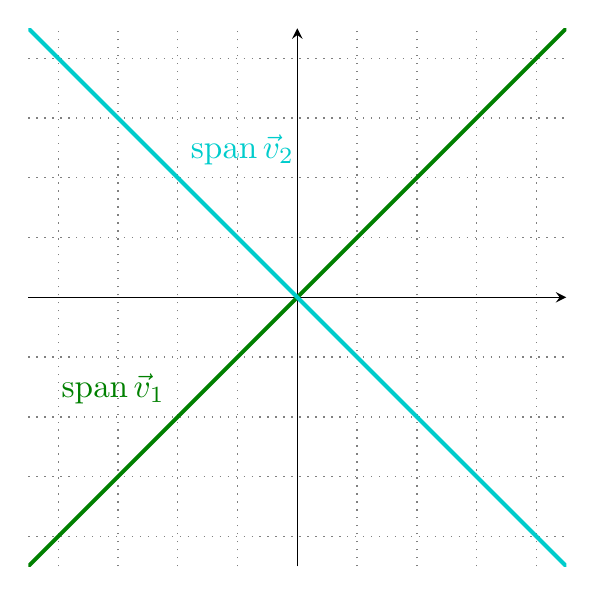
\begin{tikzpicture}[scale=1.2, >=latex]
			    \begin{axis}[scale=1,
					    axis equal image,
					    axis lines=middle,
					    axis line style = {black},
					    tick style={draw=none},
					    yticklabels={,,},
					    xticklabels={,,},
					 xmin=-4.5,
					 xmax=4.5,
					 ymin=-4.5,
					 ymax=4.5,
					 major grid style={dotted, gray},
					 xtick={-10,-9,...,10},
					 ytick={-10,-9,...,10},
					 grid=both,
					 anchor=origin]

				    \draw[Green, very thick] (-5,-5) -- (5,5) node[pos=.3, above left] {$\Span\Set{\vec v_1}$};
				    \draw[cyan!80!black, very thick] (-5,5) -- (5,-5) node[pos=.3, above right] {$\Span\Set{\vec v_2}$};
			    \end{axis}
				\end{tikzpicture}
			\end{solution}
		\item Describe $\Span\Set{\vec v_1,\vec v_2}$.
			\begin{solution}
				$\Span\Set{\vec v_1,\vec v_2} = \R^2$

				We can see this since for any $\mat{x\\y} \in \R^2$,
				\[
					\mat{x\\y}
					=\frac{x}{2}\left(\mat{1\\1}+\mat{1\\-1}\right)+\frac{y}{2}\left(\mat{1\\1}-\mat{1\\-1}\right)
					=\frac{x+y}{2}\vec v_1 + \frac{x-y}{2}\vec v_2
				\]
			\end{solution}
		\item Describe $\Span\Set{\vec v_1,\vec v_3}$.
			\begin{solution}[inline]
				$\Span\Set{\vec v_1,\vec v_3} = \Span\Set{\vec v_1}$,
				a line through the origin with direction vector $\vec v_1$.
			\end{solution}
		\item Describe $\Span\Set{\vec v_1,\vec v_2,\vec v_3}$.
			\begin{solution}[inline]
				$\Span\Set{\vec v_1,\vec v_2,\vec v_3} = \Span\Set{\vec v_1,\vec v_2} = \R^2$
			\end{solution}
	\end{parts}

	\begin{bookonly}\begin{center}\doublegrid\end{center}\end{bookonly}


\begin{lesson}
	\Title{Span, Translated Span}

	\Heading{Textbook}
	Module 3

	\Heading{Objectives}
	\begin{itemize}
		\item Explain why spans always go through the origin.
		\item Express lines or planes through the origin as spans.
		\item Express lines or planes not through the origin as translated spans.
	\end{itemize}

	\Heading{Motivation}
	Translated spans link vector form of lines and planes with sets and spans.
	Soon we will have the vocabulary of linear independence and be able to
	talk about independent direction vectors of a plane, but right now just connecting
	the concepts and notation is enough.

\end{lesson}

	\bookonlynewpage
	\question
	\begin{annotation}
		\begin{goals}
			\Goal{Connect geometric figures to spans.}

			The goal of this problem is to
			\begin{itemize}
				\item Identify a relationship between lines and spans.
				\item Describe a line through the origin as a span.
				\item Identify when a line cannot be described as a span.
				\item Apply the definition of $\Span X$ even when $X$ is infinite.
			\end{itemize}
		\end{goals}

		\begin{notes}
			\begin{itemize}
				\item The lines are not written in $y=mx+b$ form on purpose.
					We avoid this form in linear algebra since it cannot
					describe all lines.
				\item Part 3 will really stretch their minds. Students at this point are not used
					to applying definitions. They will have a conception of $\Span X$
					where $X$ is finite and will forget the definition because
					this conception is ``good enough''. This question forces
					them to think back to the definition.
			\end{itemize}
		\end{notes}
	\end{annotation}
	\label{linesAsSpans}
	Let $\ell_1\subseteq \R^2$ be the line with equation $x-y=0$ and $\ell_2\subseteq\R^2$
	the line with equation $x-y=4$.
	\begin{parts}
		\item If possible, describe $\ell_1$ as a span. Otherwise explain why
			it's not possible.
			\begin{solution}
				$\ell_1 = \Span\Set*{\mat{1\\1}}$, since $\mat{x\\y} \in \ell_1$
				if and only if $x = y$, which in turn is true if and only if it
				is a scalar multiple of $\mat{1\\1}$.
			\end{solution}
		\item If possible, describe $\ell_2$ as a span. Otherwise explain why it's
			not possible.
			\label{linesAsSpans.2}
			\begin{solution}
				This is not possible. $\mat{0\\0}$ is an element of	the span of
				\emph{any} set of vectors, since we can use all zeroes as the
				scalars in a linear combination, but $\mat{0\\0} \notin \ell_2$.
			\end{solution}
		\item Does the expression $\Span(\ell_1)$ make sense? If so, what is it?
			How about $\Span(\ell_2)$?
			\begin{solution}
				Both of these expressions do make sense. One can compute the span
				of any set of vectors, and these lines are just special set of
				points in $\R^2$ which we are already used to thinking of as vectors.

				$\Span(\ell_1) = \ell_1$, since all of the vectors on
				the line $\ell_1$ are already multiples of $\mat{1\\1}$, as we
				discovered earlier.

				$\Span(\ell_2)$ equals all of $\R^2$. It's easy to see that the
				vectors $v = \mat{4\\0}$ and $w = \mat{0\\-4}$ are both on $\ell_2$,
				and the span of these two vectors alone is all of $\R^2$.
			\end{solution}
	\end{parts}


	\bookonlynewpage
	\SavedDefinitionRender{SetAddition}


	\question
	\begin{annotation}
		\begin{goals}
			\Goal{Describing geometry using sets.}

			The goal of this problem is to
			\begin{itemize}
				\item Practice applying a new definition in a familiar context ($\R^2$).
				\item Gain an intuitive understanding of set addition.
				\item Describe lines that don't pass through $\vec 0$ using
					a combination of set addition and spans.
			\end{itemize}
		\end{goals}

		\begin{notes}
			\begin{itemize}
				\item Set addition will be brand new to most students, even
					those with a linear algebra background.
				\item Special care must be taken to differentiate
					$\vec a+\vec b$ and $\{\vec a\}+\{\vec b\}$.
				\item We will use set addition mainly as a mathematical
					notation to describe translated spans. In this
					case the summands will be an infinite set
					and a singleton. There is no need to explore the sum
					of two infinite sets.
			\end{itemize}
		\end{notes}
	\end{annotation}
	Let $A=\Set*{\mat{1\\2}}$, $B=\Set*{\mat{1\\1},\mat{1\\-1}}$,
	and $\ell=\Span\Set*{\mat{1\\-1}}$.
	\begin{parts}
		\item Draw $A$, $B$, and $A+B$ in the same picture.
			\begin{solution}
				\begin{tikzpicture}[scale=1.2, >=latex]
			    \begin{axis}[scale=1,
					    axis equal image,
					    axis line style={black},
					    axis lines=middle,
					    tick style={draw=none},
					    yticklabels={,,},
					    xticklabels={,,},
					 xmin=-4.5,
					 xmax=4.5,
					 ymin=-4.5,
					 ymax=4.5,
					 major grid style={dotted, gray},
					 xtick={-10,-9,...,10},
					 ytick={-10,-9,...,10},
					 grid=both,
					 anchor=origin]

				    %\draw[Green, very thick] (-5,0) -- (5,0) node[near end, below] {$H$};
				    %\draw[cyan!80!black, very thick] (0,-5) -- (0,5) node[near end, right] {$V$};
				    %\draw[orange!80!black, very thick] (-5,-5) -- (5,5) node[near end, below right] {$D$};


				    \fill[fill=Green] (1,2) circle[radius=2pt] node[left] {\color{Green}$A$};
				    \fill[fill=Red]
				    	(1,1) circle[radius=2pt]
				    	(1,-1) circle[radius=2pt] node[below right] {\color{Red}$B$}
				    ;
				    \fill[fill=Blue]
				    	(2,3) circle[radius=2pt]
				    	(2,1) circle[radius=2pt] node[below right] {\color{Blue}$A+B$}
				    ;
			    \end{axis}
			\end{tikzpicture}
			\end{solution}
		\item Is $A+B$ the same as $B+A$?
			\begin{solution}
				Yes. Since $A$ and $B$ are such small sets we could just
				compute all the vectors in $A+B$ and $B+A$ and see that they're
				equal. However, we know that real numbers can be added up in any
				order, and the coordinates of an element of $A+B$ or $B+A$ are
				simply sums of the corresponding coordinates of elements of $A$ and $B$.
			\end{solution}
		\item Draw $\ell+A$.
			\begin{solution}
				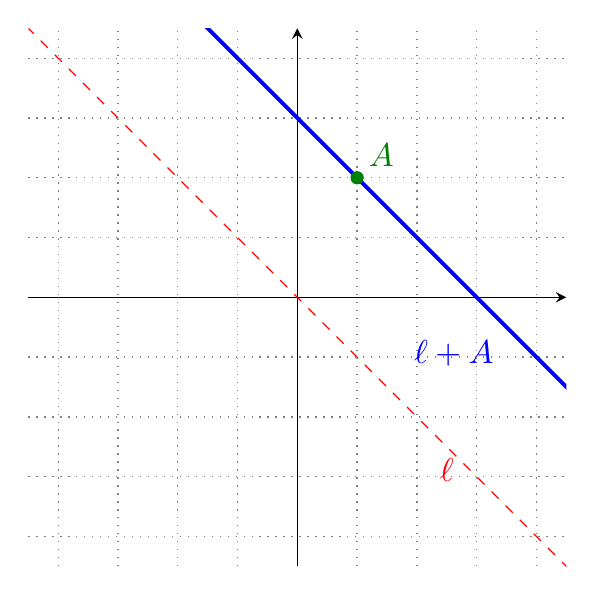
\begin{tikzpicture}[scale=1.2, >=latex]
			    \begin{axis}[scale=1,
					    axis equal image,
					    axis line style={black},
					    axis lines=middle,
					    tick style={draw=none},
					    yticklabels={,,},
					    xticklabels={,,},
					 xmin=-4.5,
					 xmax=4.5,
					 ymin=-4.5,
					 ymax=4.5,
					 major grid style={dotted, gray},
					 xtick={-10,-9,...,10},
					 ytick={-10,-9,...,10},
					 grid=both,
					 anchor=origin]

				    \draw[Red, thin, dashed] (-5,5) -- (5,-5) node[near end, below] {$\ell$};
				    \draw[Blue, very thick] (-4,7) -- (6,-3) node[near end, below left] {$\ell+A$};
				    \fill[fill=Green] (1,2) circle[radius=2pt] node[above right] {\color{Green}$A$};
			    \end{axis}
			\end{tikzpicture}
			\end{solution}
		\item Consider the line $\ell_2$ given in vector form by $\vec x=t\mat{1\\-1}+\mat{1\\2}$.
			Can $\ell_2$ be described using only a span? What about using a span
			and set addition?
			\begin{solution}
				$\ell_2$ cannot be described using only a span, for the same reason
				as the line $\ell_2$ in Problem \ref{linesAsSpans}.\ref{linesAsSpans.2}
				couldn't be. We know that the origin $\mat{0\\0}$ must be an element
				of any span, but it is not a point on $\ell_2$.

				$\ell_2$ can be described as a span plus a set addition though.
				Specifically, $\ell_2=\ell + A$.
			\end{solution}
	\end{parts}

	\begin{bookonly}\begin{center}\doublegrid\end{center}\end{bookonly}


\begin{lesson}
	\Title{Linear Independence \& Dependence}

	\Heading{Textbook}
	Module 3

	\Heading{Objectives}
	\begin{itemize}
		\item Define linear independence/dependence using spans.
		\item Pick linearly independent subsets with the same span by inspection.
		\item Explain why having a ``closed loop'' or trivial linear combination
			means a set is linearly dependent.
	\end{itemize}

	\Heading{Motivation}
	Linear independence/dependence is one of the biggest concepts in linear algebra.
	Linear independence/dependence tells us whether a set has redundant information
	in it with respect to spans. The idea of a having redundant information vs\mbox{.}
	not comes up all the time in the world (sometimes it's a plus, sometimes it's not).

	Knowing
	a set is independent tells us what its span will look like (in terms of what dimension
	it will be). It is also an abstract concept that has both a ``geometric'' definition
	and an ``algebraic'' one.
	\begin{annotation}
		\begin{notes}
			Don't define a linearly dependent \emph{set}, define
			a linearly dependent \emph{list}. Otherwise you cannot talk about
			$\mat{1\\1}$ and $\mat{1\\1}$ be linearly dependent since sets don't
			contain duplicates.
		\end{notes}
	\end{annotation}
	Geometrically, a set is linearly dependent if you can remove
	a vector without the span changing. Algebraically a set is linearly dependent if there
	is a non-trivial linear combination giving the zero vector. This lesson focuses on the
	geometric definition (with the algebraic definition coming next).

	Though the algebraic definition is easier to work with in proofs, the geometric definition
	provides intuition about how to visualize linearly
	dependent sets.

\end{lesson}

\begin{iola}
\section*{The Magic Carpet, Getting Back Home}
\addcontentsline{toc}{subsection}{The Magic Carpet Ride, Getting Back Home}
\question
	\begin{annotation}
		\begin{goals}
			\Goal{Span in higher dimensions.}

			The goal of this problem is to
			\begin{itemize}
				\item Examine subtleties that exist in three dimensions that are
					missing in two dimensions.
				\item Apply linear algebra tools to answer open-ended questions.
			\end{itemize}
		\end{goals}

		\begin{notes}
			This problem is set up to prime
			theorems about linearly dependent vectors. In particular, it
			\begin{itemize}
				\item gives an example of a non-trivial linear combination giving $\vec 0$;
				\item shows that if there is one non-trivial linear combination giving $\vec 0$,
					there are others;
				\item shows that 3 non-parallel vectors in $\R^3$ need not span $\R^3$.
			\end{itemize}

			The problem also allows linking to previous linear algebra ideas. A system
			of equations can be used to find \emph{all} non-trivial solutions, and showing
			a particular system of equations is inconsistent will show that the span
			is not $\R^3$.
		\end{notes}
	\end{annotation}
Suppose you are now in a three-dimensional world for the carpet
ride problem, and you have three modes of transportation:
\[
	\vec v_1 = \mat{1 \\1 \\ 1}\qquad
	\vec v_2 = \mat{6 \\3 \\ 8}\qquad
	\vec v_3 = \mat{4 \\1 \\ 6}
\]

You are only allowed to use each mode of transportation \textbf{once}
(in the forward or backward direction) for a fixed amount of time ($c_1$
on $\vec v_1$, $c_2$ on $\vec v_2$, $c_3$ on $\vec v_3$).

\vspace{5mm}


\begin{enumerate}
	\item  Find the amounts of time on each mode of transportation ($c_1$, $c_2$,
		and $c_3$, respectively) needed to go on a journey that starts and ends
		at home \emph{or} explain why it is not possible to do so.

	\item Is there more than one way to make a journey that meets the
		requirements described above? (In other words, are there different
		combinations of times you can spend on the modes of transportation so
		that you can get back home?) If so, how?

	\item Is there anywhere in this 3D world that Gauss
		could hide from you? If so, where? If not, why not?

	\item What is $\Span\Set*{\mat{1\\1\\1},\mat{6\\3\\8},\mat{4\\1\\6}}$?

\end{enumerate}
\end{iola}


	\begin{annotation}
		\begin{goals}
			\Goal{Geometric definition of linear independence/dependence.}
		\end{goals}

		\begin{notes}
			\begin{itemize}
				\item This definition is conceptually simple but notationally hard.
				\item The definition is phrased in terms of a list of vectors (instead of
					a set) to avoid issues with the fact that sets cannot have repeated elements. (e.g.,
					if $\vec a\neq \vec 0$, then the set $\{\vec a,\vec a\}=\{\vec a\}$ is linearly
					independent, whereas the list of vectors $\vec a,\vec a$ is linearly dependent.)
				\item Many students will not realize that $\vec v_i$ is being ``left out''
					of the span.
				\item Students might assume, for example, that $\vec v_1$ could always be removed
					from the span. This misconception is targeted in a later problem.
				\item Have students rephrase this definition in plain language.
			\end{itemize}
		\end{notes}
	\end{annotation}

	\bookonlynewpage
	\SavedDefinitionRender{LinearlyDependentIndependentGeometric}

	\question
	\begin{annotation}
		\begin{goals}
			\Goal{Apply the (geometric) definition of linear independence/dependence.}

			The goal of this problem is to
			\begin{itemize}
				\item Develop a mental picture linking linear dependence and
					``redundant'' vectors.
				\item Practice applying a new definition.
				\item Find multiple linearly independent subsets of a linearly dependent set.
			\end{itemize}
		\end{goals}

		\begin{notes}
			\begin{itemize}
				\item Students won't find this problem hard.
				\item There may be some confusion about what ``describe'' means.
			\end{itemize}
		\end{notes}
	\end{annotation}
		Let $\vec u=\mat{1\\0\\0}$, $\vec v=\mat{0\\1\\0}$, and $\vec w=\mat{1\\1\\0}$.
	\begin{parts}
		\item Describe $\Span\Set{\vec u,\vec v,\vec w}$.
			\begin{solution}
				The $xy$-plane in $\R^3$. That is, the set of all vectors in $\R^3$ with $z$-coordinate
				equal to zero.
			\end{solution}
		\item Is $\{\vec u,\vec v,\vec w\}$ linearly independent? Why or why not?
			\begin{solution}
				No. $\vec w=\vec u+\vec v$, and so $\vec w \in \Span\Set{\vec u, \vec v}$.
			\end{solution}
	\end{parts}

	Let $X=\Set{\vec u,\vec v,\vec w}$.

	\begin{parts}[resume]
		\item Give a subset $Y\subseteq X$ so that $\Span Y=\Span X$ and $Y$ is
			linearly independent.
			\begin{solution}
				$Y = \Set{\vec u,\vec v}$ is one example that works.
			\end{solution}
		\item Give a subset $Z\subseteq X$ so that $\Span Z=\Span X$ and $Z$ is
			linearly independent and $Z\neq Y$.
			\begin{solution}
				$Z = \Set{\vec u, \vec w}$ and $Z = \Set{\vec v, \vec w}$ both have
				the same span as $Y$ above.
			\end{solution}
	\end{parts}


	\bookonlynewpage
	\SavedDefinitionRender{TrivialLinearCombination}

	\question
	\begin{annotation}
		\begin{goals}
			\Goal{Link trivial/non-trivial linear combinations to linear independence/dependence.}
		\end{goals}

		\begin{notes}
			\begin{itemize}
				\item Part 2 is a chance to practice writing arguments.
				\item Many students will mistakenly assume that non-trivial means
					\emph{all} coefficients are non-zero and use this in
					their argument. Bring out this misconception.
			\end{itemize}
		\end{notes}
	\end{annotation}
		Recall $\vec u=\mat{1\\0\\0}$, $\vec v=\mat{0\\1\\0}$, and $\vec w=\mat{1\\1\\0}$.
	\begin{parts}
		\item Consider the linearly dependent
			set $\Set{\vec u,\vec v,\vec w}$ (where $\vec u,\vec v,\vec w$ are
			defined as above). Can you write $\vec 0$ as a non-trivial linear
			combination of vectors in this set?
			\begin{solution}[inline]
				$\vec 0 = \vec u + \vec v - \vec w$.
			\end{solution}
		\item Consider the linearly independent set $\Set{\vec u,\vec v}$.
			Can you write $\vec 0$ as a non-trivial linear combination of
			vectors in this set?
			\begin{solution}
				No. Suppose
				\[
					a_1 \vec u + a_2 \vec v = \vec 0
				\]
				was a non-trivial linear combination. Then at least one of $a_1$ or $a_2$
				is non-zero. If $a_1$ is non-zero, then
				\[
					\vec u = -\frac{a_2}{a_1}\vec v
				\]
				and so $\vec u\in\Span\Set{\vec v}$.
				If $a_2$ is non-zero, then
				\[
					\vec v=-\frac{a_1}{a_2}\vec u.
				\]
				and so $\vec v\in\Span\Set{\vec u}$.
				In either case, $\{\vec u,\vec v\}$ would be linearly dependent.
			\end{solution}
	\end{parts}


\begin{lesson}
	\Title{Linear Independence \& Dependence---Equivalent Definitions}

	\Heading{Textbook}
	Module 3

	\Heading{Objectives}
	\begin{itemize}
		\item Define linear independence/dependence in terms of trivial linear combinations.
		\item Explain how the geometric and algebraic definitions of linear independence/dependence relate.
		\item Explain the connection between a vector equation having multiple
			solutions and those vectors being linearly independent/dependent.
		\item Identify the largest linearly independent set that could exist in $\R^n$.
	\end{itemize}

	\Heading{Motivation}
	We've done geometry, now let's do algebra. The geometric and algebraic definitions
	are equivalent, but they suggest different consequences. The geometric definition
	of linear independence tells us about the dimension of a span. The algebraic
	definition tells us about the number of solutions to a vector equation.

\end{lesson}

	We now have an equivalent definition of linear dependence.
	\begin{annotation}
		\begin{notes}
			\begin{itemize}
				\item The algebraic definition of linear independence/dependence
					is good for proofs but hard to intuit.
			\end{itemize}
		\end{notes}
	\end{annotation}

	\bookonlynewpage
	\SavedDefinitionRender{LinearlyDependentIndependentAlgebraic}

	\question
	\begin{annotation}
		\begin{goals}
			\Goal{Link algebraic and geometric definitions of linear independence/dependence.}

			The goal of this problem is to
			\begin{itemize}
				\item Understand how the algebraic and geometric definitions of linear
					independence/dependence relate.
				\item Practice writing mathematical arguments.
			\end{itemize}
		\end{goals}

		\begin{notes}
			\begin{itemize}
				\item You could easily spend an entire class working with students
					to get well-written proofs. Be mindful of time. Since
					this is not a proofs-based course, we want to focus on the intuition here.
			\end{itemize}
		\end{notes}
	\end{annotation}
	\begin{parts}
		\item Explain how the geometric definition of linear dependence (original) implies this algebraic one (new).
			\begin{solution}
				Suppose that $\vec v_1, \vec v_2, \dots, \vec v_n$ are linearly
				dependent according to the geometric definition. Fix $i$ so that
				$\vec v_i\in \Span\Set{\vec v_1,\ldots,\vec v_{i-1},\vec v_{i+1},\ldots,\vec v_n}$.

				By the definition of $\Span$, we know that
				\[
					\vec v_i=\beta_1\vec v_1+\cdots +\beta_{i-1}\vec v_{i-1}+\beta_{i+1}\vec v_{i+1}
					+\cdots +\beta_n\vec v_{n}.
				\]
				Thus
				\[
					\vec 0 = -\vec v_i+\beta_1\vec v_1+\cdots +\beta_{i-1}\vec v_{i-1}+\beta_{i+1}\vec v_{i+1}
					+\cdots +\beta_n\vec v_{n},
				\]
				and this is a non-trivial linear combination since the coefficient of $\vec v_i$ is $-1\neq 0$.
			\end{solution}
		\item Explain how this algebraic definition of linear dependence (new) implies the geometric one (original).
			\begin{solution}
				Suppose the vectors $\vec v_1, \vec v_2, \dots, \vec v_n$ is
				linearly dependent in this new sense. That means there are
				scalars	$a_1, a_2, \dots, a_n$, at least one of which is non-zero,
				such that
				\[
					a_1 \vec v_1 + \cdots + a_n \vec v_n = 0.
				\]
				Suppose $a_i\neq 0$. Then
				\[
					\vec v_i = \tfrac{-a_1}{a_i}\vec v_1+\cdots +\tfrac{-a_{i-1}}{a_i}\vec v_{i-1}
					+\tfrac{-a_{i+1}}{a_i}\vec v_{i+1}+\cdots+\tfrac{-a_n}{a_i}\vec v_n.
				\]
				This means $\vec v_i\in \Span\Set{\vec v_1,\ldots,\vec v_{i-1},\vec v_{i+1},\ldots,\vec v_n}$,
				which is precisely the geometric definition of linear dependence.
			\end{solution}
	\end{parts}

	Since we have geometric def $\implies$ algebraic def, and algebraic def $\implies$ geometric def
	($\implies$ should be read aloud as `implies'), the two definitions
	are \emph{equivalent} (which we write as algebraic def $\iff$ geometric def).


	\displayonlynewpage
	\bookonlynewpage
	\question
	\begin{annotation}
		\begin{goals}
			\Goal{Linear dependence and infinite solutions.}

			The goal of this problem is to
			\begin{itemize}
				\item Connect linear dependence with infinite solutions.
				\item Connect linear independence with unique solutions.
			\end{itemize}
		\end{goals}

		\begin{notes}
			\begin{itemize}
				\item Part 1 won't give the students much trouble.
				\item Part 2 will be hard. The idea that you could add $\vec 0$
					but change the coefficients of a linear combination
					is hard to think of and even harder to write correctly.
			\end{itemize}
		\end{notes}
	\end{annotation}
	Suppose for some unknown $\vec u, \vec v, \vec w$, and $\vec a$,
	\[
		\vec a = 3\vec u+2\vec v +\vec w\qquad \text{and}\qquad
		\vec a = 2\vec u+\vec v -\vec w.
	\]
	\begin{parts}
		\item Could the set $\Set{\vec u,\vec v,\vec w}$ be linearly
		independent?
			\begin{solution}
				No. If both equations are true, they would combine to show
				\[
					3\vec u+2\vec v +\vec w = 2\vec u+\vec v -\vec w.
				\]
				Collecting all the terms on the left side, we get:
				\[
					\vec u + \vec v + 2\vec w = \vec 0,
				\]
				which is a non-trivial linear combination of vectors in the given
				set equalling the zero vector.
			\end{solution}
	\end{parts}
	Suppose that
	\[
		\vec a = \vec u+6\vec r-\vec s
	\]
	is the \emph{only} way to write $\vec a$ using $\vec u,\vec r,\vec s$.
	\begin{parts}[resume]
		\item Is $\Set{\vec u,\vec r,\vec s}$ linearly independent?
			\begin{solution}
				Yes. If it were not, there would exist scalars $a_1, a_2, a_3$,
				not all of which are zero, such that:
				\[
					a_1 \vec u + a_2 \vec r + a_3\vec s = \vec 0.
				\]
				But then
				\[
					\vec u+6\vec r-\vec s + (a_1 \vec u + a_2 \vec r + a_3\vec s)
				\]
				would be another way to write $\vec a$ using only the same three
				vectors.
			\end{solution}
		\item Is $\Set{\vec u,\vec r}$ linearly independent?
			\begin{solution}
				Yes. If it were not, we would necessarily have $\vec u = \beta \vec r$
				for some scalar $\beta$. But then
				\[
					(\beta + 6) \vec r - \vec s
				\]
				would be another way to write $\vec a$ using only the same three
				vectors.
			\end{solution}
		\item Is $\Set{\vec u,\vec v,\vec w,\vec r}$ linearly independent?
			\begin{solution}
				No. We know from earlier that $\vec u+\vec v+2\vec w=\vec 0$, and
				so $\vec u+\vec v+2\vec w+0\vec r=\vec 0$ is a non-trivial linear
				combination of the vectors in this set that equals the zero vector.
			\end{solution}
	\end{parts}


\begin{iola}
\section*{Linear Independence and Dependence, Creating Examples}
\addcontentsline{toc}{subsection}{Linear Independence and Dependence, Creating Examples}
\question


\begin{enumerate}
	\item Fill in the following chart keeping track of the strategies you used to generate
examples.

\vspace{2mm}

\begin{center}
	\newcommand\emptybox{\begin{bookonly}\makebox(150,80){}\end{bookonly}}
\begin{tabular}{|c|c|c|}
	\hline
	&Linearly independent & Linearly dependent \\
	\hline
	A set of 2 vectors in $\R^2$ &\emptybox&\emptybox\\
	\hline
	A set of 3 vectors in $\R^2$ &\emptybox&\\
	\hline
	A set of 2 vectors in $\R^3$ &\emptybox&\\
	\hline
	A set of 3 vectors in $\R^3$ &\emptybox&\\
	\hline
	A set of 4 vectors in $\R^3$ &\emptybox&\\
	\hline
\end{tabular}
\end{center}

		\item Write at least two generalizations that can
			be made from these examples and the strategies you
			used to create them.
	\begin{annotation}
		\begin{notes}
			\begin{itemize}
				\item Make sure ``more than $n$ vectors in $\R^n$
					is linearly dependent'' comes out.
			\end{itemize}
		\end{notes}
	\end{annotation}

\end{enumerate}

\end{iola}


\begin{module}
	\Title{Dot Products \& Normal Forms}

	In this module you will learn
	\begin{itemize}
		\item Geometric and algebraic definitions of the dot product.
		\item How dot products relate to the length of a vector and the angle
			between two vectors.
		\item The \emph{normal form} of lines, planes, and hyperplanes.
	\end{itemize}

	Let $\vec a$ and $\vec b$ be vectors rooted at the same point and let
$\theta$ denote the \emph{smaller} of the
two angles between them (so $0\leq \theta \leq \pi$).
The \emph{dot product}\index{Dot product} of $\vec a$ and $\vec b$ is defined to be
\[
	\vec a\cdot \vec b=\norm{\vec a}\norm{\vec b}\cos \theta.
\]
\index[symbols]{$\vec a\cdot \vec b$}We will call this the \emph{geometric definition of the dot product}\index{Dot product!geometric definition}\index[definitions]{Dot product!geometric definition}.

\begin{center}
	\begin{tikzpicture}
		\newcommand{\tikzAngleOfLine}{\tikz@AngleOfLine}
		  \def\tikz@AngleOfLine(#1)(#2)#3{%
		  \pgfmathanglebetweenpoints{%
		    \pgfpointanchor{#1}{center}}{%
		    \pgfpointanchor{#2}{center}}
		  \pgfmathsetmacro{#3}{\pgfmathresult}%
		  }
		\newcommand{\tikzMarkAngle}[3]{
		\tikzAngleOfLine#1#2{\AngleStart}
		\tikzAngleOfLine#1#3{\AngleEnd}
		\draw #1+(\AngleStart:0.35cm) arc (\AngleStart:\AngleEnd:0.35cm);
		}
		\coordinate (A) at (2,1);
		\coordinate (B) at (.5,2);
		\coordinate (O) at (0,0);

		\draw[->,thick,myred!60!white] (0,0) -- +(A) node [midway,below right] {$\vec a$};
		\draw[->,thick,mypink] (0,0) -- +(B) node [midway,above left] {$\vec b$};
		\tikzMarkAngle{(O)}{(A)}{(B)}
		\node at ($(O)+(50:.65)$) {$\theta$};
	\end{tikzpicture}
	\hspace{1cm}
	\begin{tikzpicture}
		\newcommand{\tikzAngleOfLine}{\tikz@AngleOfLine}
		  \def\tikz@AngleOfLine(#1)(#2)#3{%
		  \pgfmathanglebetweenpoints{%
		    \pgfpointanchor{#1}{center}}{%
		    \pgfpointanchor{#2}{center}}
		  \pgfmathsetmacro{#3}{\pgfmathresult}%
		  }
		\newcommand{\tikzMarkAngle}[3]{
		\tikzAngleOfLine#1#2{\AngleStart}
		\tikzAngleOfLine#1#3{\AngleEnd}
		\draw #1+(\AngleStart:0.35cm) arc (\AngleStart:\AngleEnd:0.35cm);
		}
		\coordinate (A) at (-2,-1);
		\coordinate (B) at (.5,2);
		\coordinate (O) at (0,0);

		\draw[->,thick,myred!60!white] (0,0) -- +(A) node [midway,below right] {$\vec a$};
		\draw[->,thick,mypink] (0,0) -- +(B) node [midway,above left] {$\vec b$};
		\tikzMarkAngle{(O)}{(B)}{(A)}
		\node at ($(O)+(140:.65)$) {$\theta$};
	\end{tikzpicture}
\end{center}

The dot product is also sometimes called the \emph{scalar product}\index{Scalar product} because
the result is a scalar.

Algebraically, we can define the dot product in terms of coordinates:
\[
	\matc{a_1\\a_2\\\vdots\\a_n}\cdot \matc{b_1\\b_2\\\vdots\\b_n}
	=a_1b_1+a_2b_2+\cdots+a_nb_n.
\]
We will call this the \emph{algebraic definition of the dot product}\index{Dot product!algebraic definition}\index[definitions]{Dot product!algebraic definition}.

By switching between algebraic and geometric definitions, we can use the dot
product to find quantities that are otherwise difficult to find.
\begin{example}
	Find the angle between the vectors $\vec v=(1,2,3)$ and $\vec w=(1,1,-2)$.

	From the algebraic definition of the dot product, we know
	\[
		\vec v\cdot \vec w = 1(1)+2(1)+3(-2) = -3.
	\]
	From the geometric definition, we know
	\[
		\vec v\cdot \vec w=\norm{\vec v}\norm{\vec w}\cos\theta
		=\sqrt{14}\sqrt{6}\cos\theta=2\sqrt{21}\cos\theta.
	\]
	Equating the two definitions of $\vec v\cdot \vec w$, we see
	\[
		\cos\theta = \frac{-3}{2\sqrt{21}}
	\]
	and so $\theta=\arccos\Big(\tfrac{-3}{2\sqrt{21}}\Big)$.
\end{example}

The dot product has several interesting properties. Since the angle between
$\vec a$ and itself is $0$, the geometric definition of the dot product tells us
\[
	\vec a\cdot \vec a=\Norm{\vec a}\Norm{\vec a}\cos 0 = \Norm{\vec a}^2.
\]
In other words,
\[
	\Norm{\vec a}=\sqrt{\vec a\cdot \vec a},
\]
and so dot products can be used to compute the length of vectors\footnote{ Oftentimes in
non-geometric settings, the dot product between two vectors is defined first and then
the length of $\vec a$ is actually \emph{defined} to be $\sqrt{\vec a\cdot \vec a}$.}.

From the algebraic definition of the dot product, we can deduce several distributive laws.
Namely, for any vectors $\vec a$, $\vec b$, and $\vec c$ and any scalar $k$ we have
\[
	(\vec a+\vec b)\cdot\vec c = \vec a\cdot \vec c+\vec b\cdot \vec c\qquad
	\vec a\cdot(\vec b+\vec c)=\vec a\cdot \vec b+\vec a\cdot \vec c
\]
\[
	(k\vec a)\cdot \vec b = k(\vec a\cdot \vec b)=\vec a\cdot (k\vec b)
\]
and
\[
	\vec a\cdot \vec b=\vec b\cdot \vec a.
\]

\Heading{Orthogonality}
Recall that for vectors $\vec a$ and $\vec b$, the relationship $\vec a\cdot \vec b=0$
can hold for two reasons: (i) either $\vec a=\vec 0$, $\vec b=\vec 0$, or both
or (ii) $\vec a$ and $\vec b$ meet at $90^{\circ}$.  Thus, the dot product
can be used to tell if two vectors are perpendicular.  There is some strangeness
with the zero vector here, but it turns out this strangeness simplifies our lives
mathematically.

\SavedDefinitionRender{Orthogonal}

The definition of orthogonal encapsulates both the idea of two vectors forming
a right angle and the idea of one of them being $\vec 0$.

\medskip
Before we continue, let's pin down exactly what we mean by
the \emph{direction} of a vector.
There are many ways we could define
this term, but we'll go with the following.

\SavedDefinitionRender{Direction}

The vector $2\xhat$ points in the direction of $\xhat$ since
$\frac{1}{2}(2\xhat)=\xhat$.  Since $\frac{1}{2}>0$, $2\xhat$ also points
in the positive direction of $\xhat$. In contrast,
$-\xhat$ points in the direction $\xhat$ but not the positive direction of $\xhat$.

When it comes to the relationship between two vectors, there are two extremes: they
point in the same direction, or they are orthogonal. The dot product can be used to
tell you which of these cases you're in, and more than that, it can tell you to
what extent one vector points in the direction of another (even if they don't point in
the same direction).

\begin{example}
	Let $\vec a=\mat{1\\2}$, $\vec b=\mat{3\\3}$, $\vec c=\mat{2\\1}$, and $\vec v=\mat{3\\4}$. Which vector out of
	$\vec a$, $\vec b$, and $\vec c$ has a direction closest to the direction of $\vec v$?

	We would like to know when $\theta$, the angle between a pair of the given vectors, is smallest.
	This is equivalent to finding when $\cos\theta$ is closest to 1 (since $\cos0=1$).
    	By equating the geometric and algebraic definitions of the dot product, we know
	    \[
        	\cos\theta = \frac{\vec p\cdot\vec q}{\norm{\vec p}\norm{\vec q}}.
	    \]

    Let $\alpha$, $\beta$, and $\gamma$ be the angles between the vector $\vec v$ and
	the vectors $\vec a$, $\vec b$, $\vec c$, respectively. Computing, we find
	\begin{align*}
	    \cos \alpha &= \frac{3+8}{5\sqrt{5}}=\frac{11\sqrt{5}}{25} \approx 0.9838699101 \\
		\cos \beta &= \frac{9+12}{5\sqrt{18}} =\frac{7\sqrt{2}}{10} \approx 0.989949437\\
	    \cos \gamma &= \frac{6+4}{5\sqrt{5}}=\frac{2\sqrt{5}}{5} \approx 0.894427191.
	\end{align*}
	Since $\cos \beta$ is the closest to $1$, we know $\vec b$ has a direction closest to that of $\vec v$.
\end{example}


\Heading{Normal Form of Lines and Planes}

Let $\vec n=\mat{1\\2}$. If a vector $\vec v=\mat{v_1\\v_2}$ is orthogonal to $\vec n$, then
\[
	\vec n\cdot\vec v=v_1+2v_2=0,
\]
and so $v_1=-2v_2$. In other words, $\vec v$ is orthogonal to $\vec n$ exactly when $\vec v\in\Span\Set*{\mat{-2\\1}}$.
What have we learned? The set of all vectors orthogonal to $\vec n$ forms a line $\ell=\Span\Set*{\mat{-2\\1}}$. In
this case, we call $\vec n$ a \emph{normal vector} for $\ell$.

\begin{center}
	\begin{tikzpicture}
		\def\dotMarkRightAngle[size=#1](#2,#3,#4){%
		 \draw ($(#3)!#1!(#2)$) --
		       ($($(#3)!#1!(#2)$)!#1!90:(#2)$) --
		       ($(#3)!#1!(#4)$);
		 \path (#3) -- ($($(#3)!#1!(#2)$)!#1!90:(#2)$);
		}
		\begin{axis}[
		    anchor=origin,
		    name=plot1,
		    disabledatascaling,
		    xmin=-3,xmax=3,
		    ymin=-2,ymax=2,
			xtick={-4,...,4},
			ytick={-2,...,4},
		    x=1cm,y=1cm,
		    grid=both,
		    grid style={line width=.1pt, draw=gray!10},
		    %major grid style={line width=.2pt,draw=gray!50},
		    axis lines=middle,
		    minor tick num=0,
		    enlargelimits={abs=0.5},
		    axis line style={latex-latex},
		    ticklabel style={font=\tiny,fill=white},
		    xlabel style={at={(ticklabel* cs:1)},anchor=north west},
		    ylabel style={at={(ticklabel* cs:1)},anchor=south west}
		]
			\coordinate (A) at (1,2);
			\coordinate (O) at (0,0);
			\coordinate (B) at (2,-1);
			\dotMarkRightAngle[size=6pt](B,O,A);
			\draw[mypink, thick] ($-2*(-2,1)$) -- ($2*(-2,1)$);
			\draw[mygreen, thick, ->] (0,0) -- (1,2) node[midway, below right] {$\vec n$};
		\end{axis}
		\node[mypink, above right] at (2,-1.2) {$\ell=\Span\Set*{\mat{-2\\1}}$};
	\end{tikzpicture}
\end{center}

\SavedDefinitionRender{NormalVector}

In $\R^2$, normal vectors provide yet another way to describe lines, including lines which don't pass
through the origin.

Let $\vec n=\mat{1\\2}$ as before, and fix $\vec p=\mat{1\\1}$. If we draw the set of all vectors
orthogonal to $\vec n$ but \emph{root all the vectors at $\vec p$}, again we get a line, but this
time the line passes through $\vec p$.

\begin{center}
	\begin{tikzpicture}
		\def\dotMarkRightAngle[size=#1](#2,#3,#4){%
		 \draw ($(#3)!#1!(#2)$) --
		       ($($(#3)!#1!(#2)$)!#1!90:(#2)$) --
		       ($(#3)!#1!(#4)$);
		 \path (#3) -- ($($(#3)!#1!(#2)$)!#1!90:(#2)$);
		}
		\begin{axis}[
		    anchor=origin,
		    name=plot1,
		    disabledatascaling,
		    xmin=-2,xmax=4,
		    ymin=-1,ymax=3,
			xtick={-4,...,4},
			ytick={-2,...,4},
		    x=1cm,y=1cm,
		    grid=both,
		    grid style={line width=.1pt, draw=gray!10},
		    %major grid style={line width=.2pt,draw=gray!50},
		    axis lines=middle,
		    minor tick num=0,
		    enlargelimits={abs=0.5},
		    axis line style={latex-latex},
		    ticklabel style={font=\tiny,fill=white},
		    xlabel style={at={(ticklabel* cs:1)},anchor=north west},
		    ylabel style={at={(ticklabel* cs:1)},anchor=south west}
		]
			\begin{scope}[cm={1,0,0,1,(1,1)}]
				\coordinate (A) at (1,2);
				\coordinate (O) at (0,0);
				\coordinate (B) at (2,-1);
				\dotMarkRightAngle[size=6pt](B,O,A);
				\draw[mypink, thick] ($-2*(-2,1)$) -- ($2*(-2,1)$);
				\draw[mygreen, thick, ->] (0,0) -- (1,2) node[midway, below right] {$\vec n$};
				\fill[myorange] (0,0) node[below left] {$\vec p$} circle[radius=2pt];
			\end{scope}
		\end{axis}
		\node[mypink, above right] at (3,0) {$\ell_2=\Span\Set*{\mat{-2\\1}}+\Set*{\mat{1\\1}}$};
	\end{tikzpicture}
\end{center}

In fact, the line we get is $\ell_2=\Span\Set*{\mat{-2\\1}}+\Set*{\mat{1\\1}}=\ell+\Set{\vec p}$, which is just $\ell$ (the
parallel line through the origin) translated by $\vec p$.

Let's relate this to dot products and normal vectors. By definition, for every $\vec v\in \ell$, we have $\vec n\cdot \vec v=0$.
Since $\ell_2$ is a translate of $\ell$ by $\vec p$, we deduce the relationship that for every $\vec v\in \ell_2$,
\[
	\vec n\cdot(\vec v-\vec p) = 0.
\]
When a line is expressed as above, we say it is expressed in \emph{normal form}.

\SavedDefinitionRender{NormalFormofaLine}

Though the definition doesn't explicitly state it, if a line $\ell\in \R^2$ is expressed in normal form
as $\vec n\cdot (\vec x-\vec p)=0$, then $\vec n$ \emph{is necessarily a normal vector for $\ell$}.
(Think about what the solution set to $\vec n\cdot (\vec x-\vec p)=0$ would be if $\vec n$ happened to be $\vec 0$!)

\bigskip
What about in $\R^3$?
Fix a non-zero vector $\vec n\in\R^3$ and let $\mathcal Q\subseteq\R^3$ be the set of vectors orthogonal to $\vec n$.
$\mathcal Q$ is a plane through the origin, and again, we call $\vec n$ a \emph{normal vector}\index{Normal vector} of the plane $\mathcal Q$.


\begin{center}
\begin{tikzpicture}
	\newcommand{\RightAngle}[4][5pt]{%
        \draw ($#3!#1!#2$)
        --($ #3!2!($($#3!#1!#2$)!.5!($#3!#1!#4$)$) $)
        --($#3!#1!#4$) ;
        }
    \begin{axis}[grid=major,view={20}{40},z buffer=sort,
	    width=12cm,
	    scale mode=scale uniformly,
	    zmin=-5,zmax=5,xmin=-10,xmax=10,ymin=-10,ymax=10,
	    xticklabels={,,}, yticklabels={,,}, zticklabels={,,},
	    xtick={-10,-5,...,10}, ytick={-10,-5,...,10}
	    ]
		\addplot3 [data cs=cart,surf,domain=-10:10,samples=2, opacity=0.5]
		{.25*x+.25*y};
		\coordinate (A) at (axis cs:-4,-4,-2);
		\coordinate (N) at (axis cs:-6,-6,6);
		\coordinate (B) at (axis cs:4,4,2);
		\coordinate (C) at (axis cs:-4,4,0);

		\draw [mypink,fill] (A) circle[radius=1.5pt] node [below right] {$\vec 0$};
		\draw [->, thick] (A) -- (B) node [midway,below right] {$\vec d_1$};
		\draw [->, thick] (A) -- (C) node [midway,above left] {$\vec d_2$};
		\draw [->, thick] (A) -- (N) node [midway,left] {$\vec n$};
		\RightAngle{(N)}{(A)}{(C)}
		%\RightAngle{(N)}{(A)}{(B)}
    \end{axis}
  \end{tikzpicture}
\end{center}

In a similar way to the line, $\mathcal Q$ is the set of solutions to $\vec n\cdot \vec x=0$.
And, for any $\vec p\in\R^3$, the translated plane $\mathcal Q+\Set{\vec p}$ is the solution set to
\[
	\vec n\cdot (\vec x-\vec p)=0.
\]
Thus, we see planes in $\R^3$ have a normal form just like lines in $\R^2$ do.

\begin{example}
	Find vector form and normal form of the plane $\mathcal P$ passing
	through the points $A=(1,0,0)$, $B=(0,1,0)$ and $C=(0,0,1)$.

	To find vector form of $\mathcal P$, we need a point on the plane and
	two direction vectors.  We have three points on the plane, so we can
	obtain two direction vectors by subtracting these points in different ways.
	Let
	\[
		\vec d_1=\overrightarrow{AB} = \mat{-1\\1\\0}\qquad\vec d_2=\overrightarrow{AC}=
		\mat{-1\\0\\1}.
	\]
	Using the point $A$, we may now express $\mathcal P$ in vector form by
	\[
		\mat{x\\y\\z} = t\mat{-1\\1\\0}+s\mat{-1\\0\\1}+\mat{1\\0\\0}.
	\]

	To write $\mathcal P$ in normal form, we need to find a normal vector for $\mathcal P$.  By inspection,
	we see that $\vec n=(1,1,1)$ is a normal vector to $\mathcal P$.  (If we weren't
	so insightful, we could also solve the system $\vec n\cdot \vec d_1=0$ and $\vec n\cdot\vec d_2=0$ to find a
	normal vector.)  Now, we may express $\mathcal P$ in normal form as
	\[
		\mat{1\\1\\1}\cdot\left(\mat{x\\y\\z}-\mat{1\\0\\0}\right)=0.
	\]
\end{example}

In $\R^2$, only lines have a normal form, and in $\R^3$ only planes have a normal form. In general,
we call objects in $\R^n$ which have a normal form \emph{hyperplanes}.

\SavedDefinitionRender{Hyperplane}

Hyperplanes always have dimension one less than the space they're contained in. So, hyperplanes in
$\R^2$ are (one-dimensional) lines, hyperplanes in $\R^3$ are regular (two-dimensional) planes,
and hyperplanes in $\R^4$ are (three-dimensional) volumes.

\Heading{Hyperplanes and Linear Equations}

Suppose $\vec n,\vec p\in \R^3$ and $\vec n\neq \vec 0$. Then, solutions to
\[
		\vec n\cdot(\vec x-\vec p)=0
\]
define a plane $\mathcal P$. But, $\vec n\cdot (\vec x-\vec p)=0$
if and only if
\[
		\vec n\cdot\vec x = \vec n\cdot \vec p = \alpha.
\]
Since $\vec n$ and $\vec p$ are fixed, $\alpha$ is a constant. Expanding using
coordinates, we see
\[
		\vec n\cdot(\vec x-\vec p)=\vec n\cdot\vec x-\alpha=
		n_xx+n_yy+n_zz-\alpha=0
\]
and so $\mathcal P$ is the set of solutions to
\begin{equation}
	\label{EQScalarForm}
		n_xx+n_yy+n_zz=\alpha.
\end{equation}
Equation \eqref{EQScalarForm} is sometimes
called \emph{scalar form}\index{Plane!scalar form of}
of a plane.  For us, it will not be important to distinguish between scalar and normal form, but
what is important is that we can use the row reduction algorithm to write the complete solution
to \eqref{EQScalarForm}, and this complete solution will necessarily be written in vector form.

\begin{example}
	Let $\mathcal Q\subseteq \R^3$ be the plane passing through $\vec p$ and with normal vector $\vec n$ where
	\[
		\vec p=\mat{1\\1\\0}\qquad\text{and}\qquad\vec n=\mat{1\\1\\1}.
	\]
	Write $\mathcal Q$ in vector form.

	We know $\mathcal Q$ is the set of solutions to $\vec n\cdot (\vec x-\vec p)=0$. In scalar form, this equation
	becomes
	\[
		\vec n\cdot (\vec x-\vec p)=\vec n\cdot \vec x-\vec n\cdot \vec p = x+y+z-2=0.
	\]
	Rearranging, we see $\mathcal Q$ is the set of all solutions to
	\[
		x+y+z=2.
	\]
	Using the row reduction algorithm to write the complete solution\footnote{ In some sense, this is overkill
	because the equation corresponds to the augmented matrix $\mat{1&1&1&\!\!\!\!|\!\!\!\!&2}$, which is already row reduced.}, we get
	\[
		\mat{x\\y\\z}=t\mat{-1\\1\\0}+s\mat{-1\\0\\1}+\mat{2\\0\\0}.
	\]
\end{example}

	\begin{exercises}
	% Topics:
	% dot products, orthogonality
	% unit vectors, vector length,
	% angle between vectors, distance between vectors
	% lines, planes, hyperplanes in normal form
	\begin{problist}
		\prob  Compute the following dot products.
		\begin{enumerate}
			\item   $\mat{9\\4} \cdot \mat{10\\-3}$
			\item   $\mat{1\\36\\2} \cdot \mat{0\\0\\1}$
			\item   $\mat{7\\6\\-3} \cdot \left(\mat{5\\11\\-1} + \mat{-2\\-6\\-1}\right)$
			\item   $\mat{1\\3\\0\\-5\\5} \cdot \mat{1\\2\\2\\1\\2}$
			\item   $\frac{1}{2}\mat{2\\5\\4} \cdot \mat{1\\0\\-1}$
		\end{enumerate}
		\prob Compute the length of the following vectors.
		\begin{enumerate}
			\item $\mat{2\\0}$
			\item $\mat{1\\2\\3}$
			\item $4\mat{5\\-6\\15\\2}$
			\item $\mat{-\frac{\sqrt{10}}{10}\\-\frac{9\sqrt{10}}{50}\\\frac{12\sqrt{10}}{50}}$
			\item $\mat{\frac{1}{3}\\\frac{\sqrt{3}}{3}\\0\\-\frac{1}{3}\\\frac{2}{3}}$
		\end{enumerate}
		\prob Find the cosine of the angle between the following vectors.
		\begin{enumerate}
			\item $\mat{1\\0}$ and $\mat{-3\\4}$
			\item $\mat{1\\0\\1}$ and $\mat{-5\\4\\-3}$
			\item $\mat{1\\2\\3}$ and $\mat{-1\\-1\\2}$
			\item $\mat{2\\4\\6}$ and $\mat{\frac{3}{2}\\3\\\frac{9}{2}}$
			\item $\mat{0\\1\\0\\1}$ and $\mat{-1\\1\\3\\0}$
		\end{enumerate}
		\prob For each vector, find two \emph{unit} vectors orthogonal to it
		\begin{enumerate}
			\item $\mat{0\\1}$
			\item $\mat{1\\2}$
			\item $\mat{1\\3\\5}$
			\item $\mat{-13\\-4\\5}$
			\item $\mat{0\\1\\1\\\frac{1}{2}}$
		\end{enumerate}

		\prob Compute the distance between the following vectors
		\begin{enumerate}
			\item $\mat{-1\\1}$ and $\mat{-1\\-4}$
			\item $\mat{2\\-6\\5}$ and $\mat{-4\\7\\-3}$
			\item $\mat{1\\1\\1}$ and $\mat{-1\\-1\\-1}$
			\item $\mat{6\\0\\2\\1}$ and $\mat{0\\1\\3\\-1}$
			\item $\mat{0\\0\\0\\0\\0}$ and $\mat{1\\1\\1\\1\\1}$
		\end{enumerate}

		\prob
		\begin{enumerate}
			\item Which vector out of $\mat{1\\0}$, $\mat{0\\1}$, and $\mat{4\\1}$
			has a direction closest to $\mat{3\\5}$?
			\item Which vector out of $\mat{2\\3\\4}$, $\mat{1\\-1\\-1}$, and $\mat{-3\\0\\1}$
			has a direction closest to $\mat{1\\0\\1}$?
		\end{enumerate}

		\prob
		\begin{enumerate}
			\item Find vector form and normal form of the plane $\mathcal P$ passing
			through the points $A=(2,0,0)$, $B=(0,3,0)$ and $C=(0,0,-1)$.
			\item Find vector form and normal form of the plane $\mathcal Q$ passing
			through the points $D=(1,1,1)$, $E=(1,-2,1)$ and $F=(0,12,0)$.
		\end{enumerate}

		\prob
		\begin{enumerate}
			\item Let $\mathcal A\subseteq \R^3$ be the plane passing through $\mat{0\\1\\1}$
			and with normal vector $\mat{-1\\-1\\-1}$. Write $\mathcal A$ in vector form.
			\item Let $\mathcal B\subseteq \R^3$ be the plane passing through $\mat{1\\2\\3}$
			and with normal vector $\mat{1\\-1\\0}$. Write $\mathcal B$ in vector form.
		\end{enumerate}

		\prob Find unit vectors in the same direction as the following vectors.
		\begin{enumerate}
			\item $\mat{90\\0}$
			\item $\mat{16\\4}$
			\item $\mat{11\\0\\13}$
			\item $\mat{3\\5\\9}$
			\item $\mat{0\\1\\0\\-1}$
			\item $\mat{434\\1337\\1999\\4568}$
		\end{enumerate}

		\prob
		\begin{enumerate}
			\item
			\label{under-add}
			\begin{enumerate}
				\item Compute $\left(\mat{1\\2} + \mat{3\\4}\right) \cdot \mat{5\\6}$
				\item Compute $\mat{1\\2} \cdot \mat{5\\6} + \mat{3\\4} \cdot \mat{5\\6}$
				\item Compare the 2 previous parts of this question. Are they similar?
			\end{enumerate}
			\item
			Do our findings from question \ref{under-add} apply to $(\vec x + \vec y) \cdot \vec u$
			for arbitrary vectors $\vec x$, $\vec y$, and $\vec u$?
			\item
			\label{under-mult}
			\begin{enumerate}
				\item Compute $\left(6\mat{2\\3}\right) \cdot \mat{4\\5}$
				\item Compute $6\left(\mat{2\\3} \cdot \mat{4\\5}\right)$
				\item Compare the 2 previous parts of this question. Are they similar?
				 Are they similar?
			\end{enumerate}
			\item
			Do our findings from question \ref{under-mult} apply to $(k\vec x) \cdot \vec y$
			for arbitrary vectors $\vec x$, $\vec y$, and scalar $k$?
			\item
			Can we show anything about $(k\vec x + \vec y) \cdot \vec u$?
			Does this also apply to $\vec u \cdot (k\vec x + \vec y)$?
		\end{enumerate}


	\end{problist}
\end{exercises}

\end{module}

\begin{lesson}
	\Title{Dot Product, Orthogonality}

	\Heading{Textbook}
	Module 4

	\Heading{Objectives}
	\begin{itemize}
		\item Compute the dot product of two vectors.
		\item Compute the length of a vector.
		\item Find the distance between two vectors.
		\item Define what it means for vectors to be orthogonal.
		\item Interpret the sign of the dot product geometrically.
		\item Create a unit vector in the direction of another.
	\end{itemize}

	\Heading{Motivation}
	Studying $\R^n$ we're in a natural inner product space with lengths and
	angles. The dot product allows us to get at lengths and angles. It will
	also give an alternative way to compute matrix products (dot product with rows
	instead of linear combination of columns).

	Most importantly, the dot product tells us how much two vectors point in
	the same direction as well as when they're orthogonal.

\end{lesson}


	\bookonlynewpage
\section*{Dot Product}
	\begin{annotation}
		\begin{notes}
			\begin{itemize}
				\item It'd be great to say $\norm{\vec v}=\sqrt{\vec v\cdot \vec v}$,
					but that would make the geometric definition of the dot product circular.
			\end{itemize}
		\end{notes}
	\end{annotation}

	\SavedDefinitionRender{Norm}

	\begin{annotation}
		\begin{notes}
			\begin{itemize}
				\item The two definitions are useful in different contexts.
				\item Students will gravitate towards the algebraic definition because
					it has an easier formula. Emphasize that if they don't know
					both definitions, there will be problems they can't solve.
			\end{itemize}
		\end{notes}
	\end{annotation}

	\SavedDefinitionRender{DotProduct}

	\question
	\begin{annotation}
		\begin{goals}
			\Goal{Practicing dot products.}

			The goal of this problem is to
			\begin{itemize}
				\item Use both the algebraic and geometric definitions of the dot product
					as appropriate to compute dot products.
				\item Gain an intuition that positive dot product
					means ``pointing in similar directions'', negative dot product
					means ``pointing in opposite directions'', and zero dot product
					means ``pointing in orthogonal directions''.
			\end{itemize}
		\end{goals}

		\begin{notes}
			\begin{itemize}
				\item For part 3(d), some students will suggest a vector
					that ``points out of the page''. This is a great idea!
					Except that such a vector would have the wrong number of components,
					so the dot products wouldn't be defined.
				\item For part 4, students will try to solve an equation. Encourage them
					to guess-and-check instead. It will be much faster.
			\end{itemize}
		\end{notes}
	\end{annotation}

		Let $\vec a=\mat{1\\1}$, $\vec b=\mat{3\\1}$, and $\vec u=\mat{1\\2\\1}$.
	\begin{parts}
		\item
		\begin{enumerate}
			\item Draw a picture of $\vec a $ and $\vec b$.
				\begin{solution}
				\begin{tikzpicture}[scale=1.2, >=latex]
			    \begin{axis}[scale=.5,
					    axis equal image,
					    axis line style={black},
					    axis lines=middle,
					    tick style={draw=none},
					    yticklabels={,,},
					    xticklabels={,,},
					 xmin=-.5,
					 xmax=4.5,
					 ymin=-.5,
					 ymax=4.5,
					 major grid style={dotted, gray},
					 xtick={-10,-9,...,10},
					 ytick={-10,-9,...,10},
					 grid=both,
					 anchor=origin]

				    \draw[Red, very thick, ->] (0,0) -- (1,1) node[near end, above] {$\vec a$};
				    \draw[Blue, very thick, ->] (0,0) -- (3,1) node[near end, above] {$\vec b$};
			    \end{axis}
			\end{tikzpicture}
				\end{solution}
			\item Compute $\vec a\cdot \vec b$.
				\begin{solution}[inline]
					$\vec a\cdot \vec b = (1)(3) + (1)(1) = 4$.
				\end{solution}
			\item Find $\|\vec a\|$ and $\|\vec b\|$ and use your knowledge of
			the multiple ways to compute the dot product to find $\theta$,
			the angle between $\vec a$ and $\vec b$. Label $\theta$ on your picture.
				\begin{solution}
					$\|\vec a\| = \sqrt{(1)^2 + (1)^2} = \sqrt{2}$ and
					$\|\vec b\| = \sqrt{(3)^2 + (1)^2} = \sqrt{10}$.

					Using the two definitions of the dot product we have:
					\begin{align*}
						\vec a\cdot \vec b &= \|\vec a\|\|\vec b\|\cos \theta \\
						\implies 4 &= (\sqrt{2})(\sqrt{10}) \cos \theta \\
						\implies \theta &= \arccos\left( \frac{2}{\sqrt{5}}\right)
					\end{align*}
				\end{solution}
		\end{enumerate}


		\begin{bookonly}\scaledgrid{.6}\end{bookonly}
		\begin{bookonly}\vspace{\stretch{1}}\end{bookonly}
		\item Draw the graph of $\cos$ and identify which angles make $\cos$
			negative, zero,	or positive.
			\begin{solution}
				\begin{tikzpicture}[scale=1.2, >=latex]
			    \begin{axis}[scale=.5,
					    axis equal image,
					    axis line style={black},
					    axis lines=middle,
					    yticklabels={,,},
					    xticklabels={,,},
					 xmin=-.5,
					 xmax=6.5,
					 ymin=-1.5,
					 ymax=1.5,
					 major grid style={dotted, gray},
					 xtick={0,.7854,...,6.284},
					 xticklabels={,,$\tfrac{\pi}{2}$,,\footnotesize $\pi$,,$\tfrac{3\pi}{2}$,,\footnotesize $2\pi$},
					 ytick={-10,-9,...,10},
					 grid=both,
					 anchor=origin]

					 \addplot[domain=0:6.283,samples=100] {cos(180/3.1415*x)};
			    \end{axis}
				\end{tikzpicture}

				Cosine is positive for angles in the interval $\left(-\frac{\pi}{2},\frac{\pi}{2}\right)$,
				as well as all shifts of this interval by a multiple of $2\pi$ in
				either direction.

				$\cos$ is positive for angles in the interval $\left(\frac{\pi}{2},\frac{3\pi}{2}\right)$,
				as well as all shifts of this interval by a multiple of $2\pi$ in
				either direction.
			\end{solution}


		\begin{bookonly}\scaledshortgrid{.7}\end{bookonly}
		\bookonlynewpage
		\item Draw a new picture of $\vec a$ and $\vec b$ and on that picture draw
		\begin{enumerate}
			\item a vector $\vec c$ where $\vec c\cdot \vec a$ is negative.
			\item a vector $\vec d$ where $\vec d\cdot \vec a=0$ and $\vec d\cdot \vec b < 0$.
			\item a vector $\vec e$ where $\vec e\cdot \vec a=0$ and $\vec e\cdot \vec b>0$.
			\item Could you find a vector $\vec f$ where $\vec f\cdot \vec a=0$ and $\vec f\cdot \vec b=0$?
				Explain why or why not.
				\begin{solution}
				\begin{tikzpicture}[scale=1.2, >=latex]
			    \begin{axis}[scale=1,
					    axis equal image,
					    axis line style={black},
					    axis lines=middle,
					    tick style={draw=none},
					    yticklabels={,,},
					    xticklabels={,,},
					 xmin=-4.5,
					 xmax=4.5,
					 ymin=-4.5,
					 ymax=4.5,
					 major grid style={dotted, gray},
					 xtick={-10,-9,...,10},
					 ytick={-10,-9,...,10},
					 grid=both,
					 anchor=origin]

				    \draw[Red, very thick, ->] (0,0) -- (1,1) node[near end, above] {$\vec a$};
				    \draw[Blue, very thick, ->] (0,0) -- (3,1) node[near end, below] {$\vec b$};
				    \draw[Yellow!70!black, very thick, ->] (0,0) -- (-2,0) node[near end, below] {$\vec c$};
				    \draw[Orange, very thick, ->] (0,0) -- (-2,2) node[near end, below] {$\vec d$};
				    \draw[Green, very thick, ->] (0,0) -- (2,-2) node[near end, below] {$\vec e$};
			    \end{axis}
			\end{tikzpicture}

					(d) $\vec f = \vec 0$ is the only possibility. For any vector
					$\vec f = \mat{x\\y}$, we can compute:
					\[
						\vec f\cdot \vec a = x + y
						\qquad \text{and} \qquad
						\vec f\cdot \vec b = 3x + y.
					\]
					If these both equal zero, the first equation says that $y = -x$,
					and in turn the second one says $x = 0$ (and so $y = 0$ as well).
				\end{solution}
		\end{enumerate}

		\item Recall the vector $\vec u$ whose coordinates are given at the beginning of this problem.
		\begin{enumerate}
			\item Write down a vector $\vec v$ so that the angle between $\vec u$
				and $\vec v$ is $\pi/2$. (Hint, how does this relate to the dot
				product?)
				\begin{solution}
					$\vec v = \mat{1\\1\\-3}$ is one such vector.

					Since $\cos(\pi/2) = 0$, from the second definition of the dot
					product above we know we are looking for a $\vec v$ such that
					$\vec u \cdot \vec v = 0$. Using the first definition of the
					dot product, we can see that the $\vec v$ given above is one
					possibility.
				\end{solution}
			\item Write down another vector $\vec w$ (in a different direction from
				$\vec v$) so that the angle between $\vec w$ and $\vec u$ is $\pi/2$.
				\begin{solution}
					$\vec w = \mat{-1\\1\\-1}$ is a possible answer.

					$\vec u \cdot \vec w = 0$, and $\vec w$ is clearly not parallel
					to $\vec v$ from above.
				\end{solution}
			\item Can you write down other vectors different than both $\vec v$
				and $\vec w$ that still	form an angle of $\pi/2$ with $\vec u$?
				How many such vectors are there?
				\begin{solution}
					Yes. $\mat{0\\2\\-4}$ is one possibility.

					There are actually infinitely many such vectors; any linear
					combination of $\vec w$ and $\vec v$ will work.

					To see this, note that any such vector $\vec x$ is of the form
					\[
						\vec x = t \mat{1\\1\\-3} + s \mat{-1\\1\\-1}
						= \matc{t-s\\t+s\\-3t-s},
					\]
					for scalars $t$ and $s$. We can then compute
					\[
						\vec u \cdot \vec x = (1)(t-s) + (2)(t+s) + (1)(-3t-s) = 0,
					\]
					and so any such vector $\vec x$ forms an angle of $\pi/2$
					with $\vec u$.
				\end{solution}
		\end{enumerate}
	\end{parts}


	\begin{bookonly}\singlegrid\end{bookonly}

	\bookonlynewpage
	\displayonlynewpage
	\begin{theorem}
		For a vector $\vec v\in \R^n$, the formula
		\[
			\|\vec v\| = \sqrt{\vec v\cdot \vec v}
		\]
		always holds.
	\end{theorem}

	\SavedDefinitionRender{Distance}

	\SavedDefinitionRender{UnitVector}

	\question
	\begin{annotation}
		\begin{goals}
			\Goal{Practice using norms.}

			The goal of this problem is to
			\begin{itemize}
				\item Practice finding the distance between two vectors.
				\item Produce a unit vector pointing in the same direction as another vector.
				\item Intuitively apply the triangle inequality: $\norm{\vec a+\vec b}\leq \norm{\vec a}+\norm{\vec b}$.
			\end{itemize}
		\end{goals}

		\begin{notes}
			\begin{itemize}
				\item Part 1 will be easy.
				\item Many will have trouble with part 2. Encourage them to write definitions! $\vec a$ is
					in the direction of $\vec u$ if $\vec a=k\vec u$ and $\vec a$ is a unit vector if $\norm{\vec a}=1$.
					Now, solve for $k$.

					They will forget that $\sqrt{k^2}=\abs{k}$ and so there are two solutions
					unless you insist on $k\geq 0$. You could mention ``in the direction of'' vs. the
					more specific ``in the positive direction of'' if you want to have a detailed discussion.
				\item Have them draw a picture for part 3.
				\item Part 4 will be very hard. Only go into it if you have plenty of time.
			\end{itemize}
		\end{notes}
	\end{annotation}
	Let $\vec u=\mat{1\\2\\1}$ and $\vec v=\mat{1\\1\\3}$.
	\begin{parts}
		\item Find the distance between $\vec u$ and $\vec v$.
			\begin{solution}
				$\vec u - \vec v = \mat{0\\1\\-2}$, and so $\norm{\vec u-\vec v} = \sqrt{5}$.
			\end{solution}
		\item Find a unit vector in the direction of $\vec u$.
			\begin{solution}
				$\frac{1}{\sqrt{6}} \vec u = \mat{\frac{1}{\sqrt{6}}\\\frac{2}{\sqrt{6}}\\\frac{1}{\sqrt{6}}}$.

				$\norm{\vec u} = \sqrt{6}$, and so if we multiply $\vec u$ by $\frac{1}{\sqrt{6}}$,
				the length of the resulting vector will be 1.
			\end{solution}
		\item Does there exist a \emph{unit vector} $\vec x$ that is distance
			$1$ from $\vec u$?
			\begin{solution}
				No. $\norm{\vec u} = \sqrt{6}$, and so the shortest length that a
				vector whose distance from $\vec u$ is 1 can have is $\sqrt{6} - 1$,
				which is greater than 1.
			\end{solution}
		\item Suppose $\vec y$ is a unit vector and the distance between $\vec y$
			and	$\vec u$ is $2$. What is the angle between $\vec y$ and $\vec u$?
			\begin{solution}
				The angle between $\vec u$ and $\vec y$ is $\arccos\left(\frac{3}{2\sqrt{6}}\right)$.

				By assumption, $2=\norm{\vec u-\vec y}$, and so
				\begin{align*}
					4 &= \norm{\vec u-\vec y}^2\\
					&= (\vec u-\vec y)\cdot(\vec u-\vec y)\\
					&= \vec u\cdot\vec u - 2(\vec u\cdot\vec y) + \vec y\cdot\vec y\\
					&=\norm{\vec u}^2 - 2\vec u\cdot\vec y + \norm{\vec y}^2\\
					&=6 - 2\vec u\cdot\vec y + 1.
				\end{align*}
				Then we rearrange to find that $\vec u\cdot \vec y = \frac{3}{2}$.

				Using this in the second definition of the dot product, we see:
				\[
					\frac{3}{2} = \left(\sqrt{6}\right)(1) \cos \theta,
				\]
				where $\theta$ is the angle between $\vec u$ and $\vec y$.
			\end{solution}
	\end{parts}

	\bookonlynewpage
	\SavedDefinitionRender{Orthogonal}

	\question
	\begin{annotation}
		\begin{goals}
			\Goal{Apply the definition of \emph{orthogonal}.}

			The goal of this problem is to
			\begin{itemize}
				\item Gain an intuitive understanding of \emph{orthogonal vectors}.
				\item Produce orthogonal vectors via guess-and-check.
				\item Apply the Pythagorean theorem to orthogonal vectors to find lengths.
			\end{itemize}
		\end{goals}

		\begin{notes}
			\begin{itemize}
				\item It won't occur to most students that $\vec 0$ is orthogonal to everything. Make sure
					this comes up.
				\item Guessing-and-checking is a valid and useful mathematical technique. Students aren't
					comfortable with this method because there's no algorithm for it (and so it
					doesn't seem reliable and repeatable). We should change their attitude. Most problems
					in their lives won't be solved with repeatable algorithms (unless they work on
					an assembly line).
			\end{itemize}
		\end{notes}
	\end{annotation}
	\begin{parts}
		\item Find two vectors orthogonal to $\vec a=\mat{1\\-3}$.  Can you find
			two such vectors that are not parallel?
			\begin{solution}
				Two such vectors are $\mat{3\\1}$ and $\mat{-6\\-2}$.

				It is impossible for two non-parallel vectors to both be
				orthogonal to $\vec a$. If $\vec b = \mat{x\\y}$ is orthogonal to
				$\vec a$, then we must have that $x - 3y = 0$, or in other words
				that $x = 3y$. Any $\vec b$ satisfying this is a multiple of
				$\mat{3\\1}$.
			\end{solution}
		\item Find two vectors orthogonal to $\vec b=\mat{1\\-3\\4}$.  Can you
			find two such vectors that are not parallel?
			\begin{solution}
				Two such vectors are $\mat{7\\1\\-1}$ and $\mat{2\\2\\1}$.

				These two vectors are not parallel.
			\end{solution}
		\item Suppose $\vec x$ and $\vec y$ are orthogonal to each other and
			$\norm{\vec x}=5$ and $\norm{\vec y}=3$. What is the distance between
			$\vec x$ and $\vec y$?
			\begin{solution}
				The distance between them must be $\sqrt{34}$.

				One way to see this is with Pythagoras' theorem. Two perpendicular
				line segments of lengths 3 and 5 form the two shorter sides of a
				right angle triangle, and so the length of the third side is
				$\sqrt{5^2 + 3^2} = \sqrt{34}$.

				An equivalent way to see this is to use what we know about dot
				products to calculate $\norm{\vec x-\vec y}$ as follows:
				\[
					\norm{\vec x-\vec y} = \sqrt{(\vec x-\vec y)\cdot(\vec x-\vec y)}
					= \sqrt{\norm{\vec x}^2 - 2(\vec x\cdot\vec y) + \norm{\vec y}^2}
					= \sqrt{5^2 + 2(0) + 3^2},
				\]
				where in the last step we've used the fact that $\vec x$ and $\vec y$
				are orthogonal, so $\vec x\cdot\vec y = 0$.
			\end{solution}
	\end{parts}

\begin{lesson}
	\Title{Normal Form of Lines and Planes}

	\Heading{Textbook}
	Module 4

	\Heading{Objectives}
	\begin{itemize}
		\item Describe lines and planes in normal form.
	\end{itemize}

	\Heading{Motivation}
	Physics often describes surfaces in terms of normal and tangential components.
	Normal form of lines and planes is one way to get at this decomposition. Further, thinking
	about lines and planes in terms of right angles will help when visualizing orthogonal projections.

\end{lesson}

	\bookonlynewpage
	\question
	\begin{annotation}
		\begin{goals}
			\Goal{Generate lines using orthogonality.}

			The goal of this problem is to
			\begin{itemize}
				\item Visually see how the set of all vectors orthogonal to
					a given vector forms a line.
				\item Given a line defined as the set of all vectors orthogonal
					to a given vector, express the line using an equation or
					span.
			\end{itemize}
		\end{goals}

		\begin{notes}
			\begin{itemize}
				\item This problem won't be hard, so don't spend too much time on it.
				\item For part 1, students might insist on drawing arrowheads and tails
					on their vectors. This is an opportunity to discuss when you should
					draw arrowheads/tails and when you shouldn't.
			\end{itemize}
		\end{notes}
	\end{annotation}
	\begin{parts}
		\item Draw $\vec u=\mat{2\\3}$ and \emph{all} vectors orthogonal to it.
			Call this set $A$.
			\begin{solution}
				\begin{tikzpicture}[scale=1.2, >=latex]
			    \begin{axis}[scale=1,
					    axis equal image,
					    axis line style={black},
					    axis lines=middle,
					    tick style={draw=none},
					    yticklabels={,,},
					    xticklabels={,,},
					 xmin=-4.5,
					 xmax=4.5,
					 ymin=-4.5,
					 ymax=4.5,
					 major grid style={dotted, gray},
					 xtick={-10,-9,...,10},
					 ytick={-10,-9,...,10},
					 grid=both,
					 anchor=origin]

				    \draw[Red, very thick, ->] (0,0) -- (2,3) node[near end, left] {$\vec u$};
				    \draw[Green, very thick] (-6,4) -- (6,-4) node[near end, below left] {$A$};
			    \end{axis}
			\end{tikzpicture}
			\end{solution}
		\item If $\vec x=\mat{x\\y}$ and $\vec x$ is orthogonal to $\vec u$,
			what is $\vec x\cdot \vec u$?
			\begin{solution}[inline]
				$\vec x\cdot \vec u = 0$, by the definition of orthogonality.
			\end{solution}
		\item Expand the dot product $\vec u\cdot \vec x$ to get an equation for $A$.
			\begin{solution}
				$A$ is the line with vector equation $\vec x = t\mat{3\\-2}$.

				If $\vec x=\mat{x\\y} \in A$, then $\vec x\cdot\vec u = 2x + 3y = 0$.
			\end{solution}
		\item If possible, express $A$ as a span.
			\begin{solution}[inline]
				$A = \Span\Set*{\mat{3\\-2}}$.
			\end{solution}
	\end{parts}

	\begin{bookonly}\singlegrid\end{bookonly}
	\bookonlynewpage
	\displayonlynewpage
	\SavedDefinitionRender{NormalVector}

	\question
	\begin{annotation}
		\begin{goals}
			\Goal{Express lines in normal form.}

			The goal of this problem is to
			\begin{itemize}
				\item Express lines, including lines that don't pass through $\vec 0$,
					in normal form.
				\item See the $\vec q$ in $\vec n\cdot (\vec x-\vec q)=0$ is similar
					to the $\vec p$ in the vector form $\vec x=t\vec d+\vec p$ in
					that it accommodates lines that don't pass through $\vec 0$.
				\item Use the dot product to represent a line compactly.
			\end{itemize}
		\end{goals}

		\begin{notes}
			\begin{itemize}
				\item In part 2 there may be some lingering confusion about the difference between
					a vector and a point. In particular, $\vec u-\vec p$ is a direction vector for $\ell_2$,
					but is not \emph{contained in} $\ell_2$.
				\item In part 3, have a discussion about the role that $\vec q$ plays. Namely,
					that it ``translates'', in a similar way that $\vec p$ in the vector
					form $\vec x=t\vec d+\vec p$ translates.

					However, be careful about the discussion here. Students may find it very
					confusing that we ``subtract $\vec q$'' to translate in normal form, whereas in
					vector form we add $\vec p$. Have a good explanation prepared if you go
					down this route.
			\end{itemize}
		\end{notes}
	\end{annotation}
	Let $\vec d=\mat{1\\2}$ and $\vec p=\mat{1\\-1}$, and define the lines
	\[
		\ell_1 = \Span\Set{\vec d}\qquad\text{and}\qquad \ell_2=\Span\Set{\vec d}+\Set{\vec p}.
	\]
	\begin{parts}
		\item Find a vector $\vec n$ that is a normal vector for both $\ell_1$
			and	$\ell_2$.
			\begin{solution}
				$\vec n=\mat{2\\-1}$ is one possibility.

				This vector is orthogonal to $\vec d$, which is a direction
				vector for both lines.
			\end{solution}
		\item Let $\vec v\in \ell_1$ and $\vec u\in \ell_2$.
			What is $\vec n\cdot \vec v$? What about $\vec n\cdot (\vec u-\vec p)$? Explain using a picture.
			\begin{solution}
				$\vec n\cdot \vec v =\vec n\cdot(\vec u-\vec p)= 0$.

				This is because any $\vec v \in \ell_1$ is a multiple
				of $\vec d$, which is orthogonal to $\vec n$. Similarly, for any $\vec u\in \ell_2$,
				the vector $\vec u-\vec p$ is a direction vector for $\ell_2$, and so it is orthogonal to $\vec n$.

				$\vec n\cdot \vec u=3$, since any such $\vec u$ is of the form
				$\vec u=\vec p+t\vec d$ for some scalar $t$, and so
				\[
					\vec n\cdot \vec u
					=\vec n\cdot (\vec p+t\vec d)
					=\vec n\cdot \vec p+t(\vec n\cdot \vec d)
					=3+t(0)
					=3.
				\]
			\end{solution}
		\item A line is expressed in \emph{normal form} if it is represented by
			an equation of the form $\vec n\cdot (\vec x-\vec q)=0$ for some
			$\vec n$ and $\vec q$. Express $\ell_1$ and $\ell_2$ in normal form.
			\begin{solution}
				A normal form of $\ell_1$ is $\mat{2\\-1}\cdot\vec x=0$.

				A normal form of $\ell_2$ is $\mat{2\\-1}\cdot\left(\vec x-\mat{1\\-1}\right)=0$.
				In the previous part we saw that $\vec n\cdot \vec x=\vec n\cdot \vec p$
				for all $\vec x\in \ell_2$, or in other words $\vec n\cdot (\vec x-\vec p) = 0$.
			\end{solution}
		\item Some textbooks would claim that $\ell_2$ could be expressed in normal form as {\color{cyan}$\mat{2\\-1}\cdot \vec x=3$}.
			How does this relate to the $\vec n\cdot(\vec x-\vec p)=0$ normal form? Where does the $3$ come from?
			\begin{solution}
				Let $\vec n=\mat{2\\-1}$ and let $\vec x\in \ell_2$. From the previous part, we know
				\[
					0=\vec n\cdot (\vec x-\vec p)
					=\vec n\cdot \vec x-\vec n\cdot \vec p
					=\vec n\cdot \vec x-3.
				\]
				Therefore
				\[
					\vec n\cdot \vec x= 3.
				\]
			\end{solution}
	\end{parts}

	\bookonlynewpage
	\question
	\begin{annotation}
		\begin{goals}
			\Goal{Planes in normal form.}

			The goal of this problem is to
			\begin{itemize}
				\item Observe that the set of all vectors orthogonal to another in $\R^3$
					is a plane.
				\item Translate descriptions of sets into precise mathematical statements using
					set-builder notation.
				\item Express a plane in multiple ways.
			\end{itemize}
		\end{goals}

		\begin{notes}
			\begin{itemize}
				\item Students have already worked with this plane in problem \ref{ProbPlane},
					but they won't remember. Emphasize part 1 and go quickly through the other parts,
					referring to problem \ref{ProbPlane} if needed.
			\end{itemize}
		\end{notes}
	\end{annotation}
	Let $\vec n=\mat{1\\1\\1}$.
	\begin{parts}
		\item Use set-builder notation to write down the set, $X$, of
			all vectors orthogonal to $\vec n$. Describe this set
			geometrically.
			\begin{solution}
				$X = \Set*{\vec x\in \R^3 \given \vec x\cdot \vec n = 0}$.

				Geometrically, this is a plane through the origin and
				orthogonal to $\vec n$.
			\end{solution}
		\item Describe $X$ using an equation.
			\begin{solution}[inline]
				$x+y+z=0$.
			\end{solution}
		\item Describe $X$ as a span.
			\begin{solution}[inline]
				$X = \Span\Set*{\mat{1\\-1\\0},\mat{1\\0\\-1}}$ is one way to do this.
			\end{solution}
	\end{parts}


\begin{module}
	\Title{Projections \& Vector Components}

	In this module you will learn
	\begin{itemize}
		\item The definition of the projection of a vector onto a set and the definition of the vector component of one vector
			in the direction of another.
		\item The relationship between projection, orthogonality, and vector components.
		\item How to project a vector onto a line.
	\end{itemize}

	Consider the following situation: you're designing a 3d video game, but your uses only have 2d screens.
Or, you have a 900-dimensional dataset, but you want to visualize it on a continuum (i.e., as a line). 
Each of these is an example
of finding the best approximation to particular points given some restrictions. In general, this operation
is called a \emph{projection}\footnote{ What we define as a \emph{projection} is sometimes
called an \emph{orthogonal projection} to distinguish it from other types of projections.}, 
and in the world of linear algebra, it has a very particular meaning.

\SavedDefinitionRender{Projection}

Let $\mathcal P_{xy}\subseteq\R^3$ be the $xy$-plane in $\R^3$ and let $\vec v=\mat{1\\2\\3}$. Intuitively, 
$\Proj_{\mathcal P_{xy}}\!\!\vec v$ is the ``shadow'' that  $\vec v$ would casts on ${\mathcal P_{xy}}$ if 
the sun were directly overhead.
In other words,
\[
	\Proj_{\mathcal P_{xy}}\vec v=\mat{1\\2\\0}.
\]

XXX Figure

Let $\ell_y\subseteq \R^3$ be the $y$-axis in $\R^3$. It's a little bit harder to visualize what $\Proj_{\ell_y}\vec v$
is, so let's appeal to some definitions.

By definition, every vector in $\ell_y$ takes the form $\vec u_t=\mat{0\\t\\0}$ for some $t\in \R$. The distance
between $\vec u_t$ and $\vec v$ is
\[
	\Norm{\vec u_t-\vec v}=\norm*{\mat{0\\t\\0}-\mat{1\\2\\3}} = \sqrt{1^2+(t-2)^2+3^2}.
\]
Since $(t-2)^2$ is always positive, the quantity $\sqrt{1^2+(t-2)^2+3^2}$ is minimized when $(t-2)^2=0$. That is,
when $t=2$. Thus, we see $\vec u_2$ is the closest vector in $\ell_y$ to $\vec v$ and so,
\[
	\Proj_{\ell_y}\vec v=\vec u_2=\mat{0\\2\\0}.
\]


\begin{example}
	Let $\ell\subseteq \R^2$ be the line given in vector form by $\vec x=t\mat{1\\1}+\mat{3\\-2}$,
	and let $\vec v=\mat{-1\\-1}$. Use the definition of projection to find $\Proj_\ell \vec v$.

	By definition, the distance between $\vec v$ and vectors in $\ell$ is given by
	\[
	    \Norm{\vec u-\vec v}=\norm*{\mat{t+3\\t-2}-\mat{-1\\-1}} = \sqrt{(t+4)^2+(t-1)^2}=\sqrt{2t^2+6t+17}=\sqrt{2\left(t+\frac{3}{2}\right)^2+\frac{25}{2}},
	\]
	where $t=-\frac{3}{2}$ minimizes the value of the distance. Therefore, we find 
	\[
	    \Proj_\ell \vec v=-\frac{3}{2}\mat{1\\1}+\mat{3\\-2}=\frac{1}{2}\mat{3\\-7}.
	\]
\end{example}

Every example of a projection so far shares a geometric property. In the case of lines and planes,
the vector from the tip of the projection to the original point is a normal vector for the line or plane (provided it's non-zero).

XXX Figure

Stated precisely, if $X$ is a line or plane and $\vec v\notin X$ is a vector, then $\vec v-\Proj_X\vec v$ is a
normal vector for $X$. Using this fact, we can find projections onto lines and planes without needing to compute
any distances!

\begin{example}
	Let $\ell\subseteq \R^2$ be the line given in vector form by $\vec x=t\mat{1\\1}+\mat{3\\-2}$,
	and let $\vec v=\mat{-1\\-1}$. Use the fact that $\vec v-\Proj_\ell\vec v$ is a normal vector to $\ell$
	to find Find $\Proj_\ell \vec v$.

	Since $\vec v-\Proj_\ell\vec v$ is a normal vector to $\ell$, $\vec v-\Proj_\ell\vec v$ is orthogonal to $\vec d=\mat{1\\1}$. Thus, let $\Proj_\ell\vec v = \mat{x\\y}$ for some unknown $x,y\in\R$, we have
	\begin{equation}
	\label{EQREGSYS1}
	    (\vec v-\Proj_\ell\vec v)\cdot\vec d=0 \implies \mat{-1-x\\-1-y}\cdot \mat{1\\1}=0\implies x+y=-2.
	\end{equation}
	Also, since $\Proj_\ell\vec v$ is a vector in $\ell$, $\Proj_\ell\vec v$ also satisfies
	\begin{equation}
	\label{EQREGSYS2}
	    \mat{x\\y}=t\mat{1\\1}+\mat{3\\-2}\implies
	    \sysdelim\{.
		\systeme*{
			x=t+3,
			y=t-2
		} \implies x-y=5
	\end{equation}
	Solve the two-equations system given by \eqref{EQREGSYS1} and \eqref{EQREGSYS2}, we find $\Proj_\ell\vec v = \frac{1}{2}\mat{3\\-7}$. 
\end{example}

\Heading{Projections Onto Other Sets}
For projections onto lines and planes, we can use what we know about normal vectors to simplify our life.
The same is true when projecting onto other sets, but we must always keep the definition in mind.

\begin{example}
	Let $\mathcal T\subseteq \R^2$ be the filled in triangle with vertices $\mat{0\\0}$, 
	$\mat{1\\0}$, and $\mat{0\\2}$, and let
	\[
		\vec a=\mat{1/4\\1/4}\qquad \vec b=\mat{3\\1/2}\qquad \vec c=\mat{1\\1}.
	\]
	Find $\Proj_{\mathcal T}\vec a$, $\Proj_{\mathcal T}\vec b$, and  $\Proj_{\mathcal T}\vec c$.

	XXX Finish
	XXX Figure
\end{example}

\Heading{Subtleties of Projections}
You might be wondering, what is $\Proj_X\vec v$ if $\vec v$ is equidistant from \emph{two}
closest points in $X$? Or, what if $X$ is an \emph{open} set (for example, an open interval in $\R^1$)?
Then there might not be a closest point in $X$ to $\vec v$. In both these cases, we say $\Proj_X\vec v$
is \emph{undefined}.

Formally, for a fixed set $X$, we consider $P(\vec v)=\Proj_X\vec v$ as a function that inputs and outputs
vectors. And, as a function, $P$ has a domain consisting of exactly the vectors $\vec v$ for which $P(\vec v)$
is defined. As it happens, if $X$ is a line or a plane, the domain of $P$ is all of $\R^n$, and in this text,
we will be sensible and only ask about projections that exist. 

\Heading{Vector Components}

We've seen before that dot products can be used to measure how much one
vector points in the direction of another. But, we can go further. Suppose 
$\vec v\neq \vec 0$ and $\vec u$ are vectors. We might want to \emph{decompose}
$\vec u$ into the sum of two vectors, one which is in the direction of $\vec v$
and the other which is orthogonal to $\vec v$. The tool to that does this is the \emph{vector component}.

\SavedDefinitionRender{Component}

From the definition, it's obvious that
\[
	\vec u=\Vcomp_{\vec v}\vec u + (\vec u-\Vcomp_{\vec v}\vec u)
\]
is a decomposition of $\vec u$ into the sum of two vectors, one, $\Vcomp_{\vec v}\vec u$, is in the direction of $\vec v$,
and the other, $\vec u-\Vcomp_{\vec v}\vec u$, is orthogonal to $\vec v$.

\begin{example}
	Find the vector component of $\vec a=\mat{1\\2}$ in the direction of $\vec b=\mat{1\\1}$.

    Let $\Vcomp_{\vec b}\vec a=\mat{x\\y}$ for some unknown $x,y\in\R$. 
    
    By definition, $\vec a - \Vcomp_{\vec b}\vec a$ is orthogonal to $\vec b$. That is,
    \begin{equation}
    \label{e1}
        (\vec a-\Vcomp_{\vec b}\vec a)\cdot\vec b=0. \implies \mat{1-x\\2-y}\cdot\mat{1\\1} = 0 \implies x+y=3.
    \end{equation}
    Also from the definition, $\Vcomp_{\vec b}\vec a$ is the vector in the direction of $\vec b$. Thus, for some $k\in\R$, we have
    \begin{equation}
    \label{e2}
        \Vcomp_{\vec b}\vec a = k\vec b \implies\mat{x\\y}=\mat{k\\k}\implies x-y=0.
    \end{equation}
    Therefore, solving the two-equation system given by \eqref{e1} and \eqref{e2}, we have
    \[
        \vec a-\Vcomp_{\vec b}\vec a=\frac{3}{2}\mat{1\\1}.
    \]
\end{example}

Since we'll be computing vector components often, let's try to find a formula for $\Vcomp_{\vec v}\vec u$.

By definition $\Vcomp_{\vec v}\vec u$ is a vector in the direction of $\vec v$, so
\[
	\Vcomp_{\vec v}\vec u = k\vec v.
\]
Further, from the definition $\vec u-\Vcomp_{\vec v}\vec u$ is orthogonal to $\vec v$, and so
\[
	\vec v\cdot (\vec u-\Vcomp_{\vec v}\vec u) = \vec v\cdot (\vec u-k\vec v)=\vec v\cdot \vec u-k\vec v\cdot \vec v=0,
\]
Because $\vec v\neq \vec 0$, we know $\vec v\cdot \vec v\neq 0$. Therefore, we may rearrange and solve for $k$ to find
\[
	k=\frac{\vec v\cdot \vec u}{\vec v\cdot \vec v},
\]
which means
\[
	\Vcomp_{\vec v}\vec u = \left(\frac{\vec v\cdot \vec u}{\vec v\cdot \vec v}\right)\vec v.
\]

\Heading{The Relationship Between Vector Components and Projections}

Vector components and projections onto lines are closely related. So closely related that many textbooks
use the single word \emph{projection} to talk about both vector components and projections\footnote{ We will not.}. Let's take a moment
to explore this relationship.

Let $\vec v=\mat{2\\4}$ and $\vec u=\mat{2\\-1}$ and let $\ell=\Span\Set{\vec v}$. Drawing a picture of
$\ell$, $\vec u$, and $\Proj_\ell\vec u$, we see that $\Proj_\ell\vec u$ satisfies all the properties
of $\Vcomp_{\vec v}\vec u$.

XXX Figure

Since $\ell=\Span\Set{\vec v}$ and $\Proj_\ell\vec u\in\ell$, we know that $\Proj_\ell\vec u$ is in the direction
of $\vec v$. Further, using geometric arguments, we know $\vec u-\Proj_\ell\vec u$ is a normal vector for $\ell$
and is therefore orthogonal to its direction vector $\vec v$! What's more, we didn't
use anything in particular about $\vec u$ and $\vec v$ when making this argument (other than $\vec v\neq \vec 0$). This means,
we have established a general fact. 

\begin{theorem}
	For vectors $\vec u$ and $\vec v\neq 0$, we have
	\[
		\Proj_{\Span\Set{\vec v}}\vec u=\Vcomp_{\vec v}\vec u.
	\]
\end{theorem}

This is great news because vector components are easy to compute using dot products while projections are usually hard to compute.

\begin{example}
	Compute the projection of $\vec a=\mat{3\\7}$ onto $\ell=\Span\Set*{\mat{1\\-4}}$.

	By the theorem above, let $\vec b = \mat{1\\-4}$, we have
	\[
	    \Proj_\ell \vec a = \Vcomp_{\vec b} \vec a = \left(\frac{\vec d\cdot \vec a}{\vec b\cdot \vec b}\right)\vec b = -\frac{3-28}{1+16}\mat{1\\-4}=-\frac{25}{17}\mat{1\\-4}.
	\]
\end{example}

It's worth noting, however, that vector components are equal to projections \emph{only in the case when you're
projecting onto a span}. In general, projections and vector components are unrelated. 

\begin{example}
	Let $\vec a=\mat{3\\7}$ , $\vec b=\mat{1\\-4}$, and let $\ell$ be the line given in vector form by
	$\vec x=t\vec b+\vec a$. Show that $\Proj_\ell\vec a\neq \Vcomp_{\vec b}\vec a$.

	By definition, $\Proj_{\ell}\vec a$ is the closest point in $\ell$ to $\vec a$. Since the distance is given by
	\[
	    \norm*{(t\vec b+\vec a)-\vec a}=t\norm*{\vec b}=\sqrt{17}t,
	\]
	where $t=0$ minimizes the value of the distance. Therefore, we obtain
	\[
	    \Proj_{\ell}\vec b = \vec 0 + \vec a = \mat{3\\7}.
	\]
	But by definition, $\Vcomp_{\vec b}\vec a$ is the vector in the direction of $\vec b$ so that $\vec a - \Vcomp_{\vec b}\vec a$ is orthogonal to $\vec b$. Therefore, $\Vcomp_{\vec b}\vec a$ would be the same as the example above. Thus, we find 
	\[
	    \Proj_{\ell}\vec b=\mat{3\\7}\neq-\frac{25}{17}\mat{1\\-4}=\Vcomp_{\vec b}\vec a.
	\]
	
\end{example}


	\begin{exercises}

	\begin{problist}
		\prob Let $T=\Set*{\mat{0\\0}, \mat{-1\\2}, \mat{1\\-2}}$. Find $\Proj_{T}
		\mat{3 \\ 1}$.
		\begin{solution}
			The distances from $\mat{ 3 \\ 1 }$ to $\mat{0\\0}$, $\mat{-1\\2}$,
			and $\mat{1\\-2}$ are $\sqrt{10}$, $\sqrt{17}$, and
			$\sqrt{13}$, respectively. So $\Proj_{T} \mat{3 \\ 1}= \mat{
			0 \\ 0}$.
		\end{solution}

		\prob Let $C=\Set*{ \vec v \in \R^2\given \norm{ \vec v} = 1}$ be
		the unit circle in $\R^{2}$. Find $\Proj_{C} \mat{2 \\ 0}$. Justify
		your answer.
		\begin{solution}
			Suppose $\vec v=\mat{x\\y}\in C$. We would like to minimize
			$\left \Vert \mat{ x \\ y }- \mat{ 2 \\ 0 }\right \Vert$,
			or equivalently
			$\left \Vert \mat{ x \\ y }- \mat{ 2 \\ 0 }\right \Vert^{2}$.
			This expression can be rewritten as
			\[
				\left \Vert \mat{ x \\ y }- \mat{ 2 \\ 0 }\right
				\Vert^{2} = (x-2)^{2}+y^{2} = (x^{2}+y^{2})-4x+4
			\]

			\[
				= \left\Vert \vec v \right \Vert^{2}-4x+4 = 5 - 4x.
			\]
			 Since $x \leq 1$, the above expression is minimized when
			$x = 1$ (and thus $y = 0$). That is,
			\[
				\Proj_{C} \mat{2 \\ 0}= \mat{ 1 \\ 0 }.
			\]

		\end{solution}

		\prob Let $\ell=\Span \Set*{ \mat{2 \\ 1}}$, $L=\Span \Set*{ \mat{2
		\\ 1}}+\Set*{\mat{4\\0}}$, and let $S$ be the set of convex
		linear combinations of $\mat{2 \\ 1}$ and $\mat{4 \\ 2}$. For $\vec
		v = \mat{ 1 \\ 0}$, find
		\begin{enumerate}
			\item $\Proj_{\ell} \vec v$.

			\item $\Proj_{L} \vec v$.

			\item $\Proj_{S} \vec v$.
		\end{enumerate}
		\begin{solution}

			\begin{enumerate}
				\item Let $\vec u=\mat{ 2 \\ 1 }$. Then
					$\Proj_{\ell} \vec v=t\vec u$ for some
					$t\in \R$ which minimizes


					\[
						\left \Vert \vec v - t \vec u
						\right \Vert^{2} = \left \Vert \vec
						u \right \Vert^{2} t^{2} - (2
						\vec u \cdot \vec v) t + \left \Vert
						\vec v \right \Vert^{2}.
					\]


					This quantity is minimized when
					$t = \frac{\vec u \cdot \vec v}{\left
					\Vert \vec u \right \Vert^2}= \frac{2}{5}$,
					so
					\[
						\Proj_{\ell} \vec v = \tfrac{2}{5}\vec
						u=\tfrac 15 \mat{4\\2}.
					\]


				\item Let $\vec u=\mat{ 2 \\ 1 }$. Then
					$\Proj_{L} \mat{ 1 \\ 0}=\mat{4\\0}+t\vec
					u$
					for some $t\in \R$ which minimizes
					\[
						\left \Vert \mat{ 1 \\ 0}- \mat{4\\0}-t
						\vec u \right \Vert^{2} = (-3-2t)^{2}+(0-t)^{2}
					\]

					\[
						= 9+12t+5t^{2}.
					\]
					 The quantity $9+12t+5t^{2}=5(t+\frac 65
					)^{2}+\frac 95$ is minimized when $t = -\frac
					65$, so
					\[
						\Proj_{L} \vec v = \mat{4\\0}-\tfrac
						65\vec u=\tfrac 15 \mat{8\\-6}
					\]


				\item The set $S$ is equal to $\Set{t \vec u: 1
					\leq t \leq 2}$ (check this), and so $S\subseteq
					\ell$. We found
					$\Proj_{\ell}\vec v=\mat{4/5\\2/5}$
					which is not in $S$. Therefore, $\Proj_{S}\vec
					v$ must be one of the endpoints of $S$.
					Checking both endpoints, we conclude
					$\Proj_{S} \vec v = \mat{2 \\ 1}$.
			\end{enumerate}
		\end{solution}

		\prob Let $T$ be the set of convex linear combinations of
		$\Set*{\mat{1\\1}, \mat{-1\\1},\mat{-1\\-2}}$. Find $\Proj_{T}(\vec
		v)$, for
		\begin{enumerate}
			\item $\vec v = \mat{3\\3}$

			\item $\vec v = \mat{0\\0}$

			\item $\vec v = \mat{1\\-2}$

			\item $\vec v = \mat{0\\-4}$
		\end{enumerate}
		\begin{solution}
			Geometrically, $T$ is a filled in triangle with vertices
			$\mat{1\\1}, \mat{-1\\1}$ and $\mat{-1\\-2}$. So for points
			outside the triangle, the closest point in $T$ will be on
			the nearest side of $T$, and so we can project onto $T$
			by projecting onto line segments.


			\begin{enumerate}
				\item $\Proj_{T} \mat{3\\3}= \mat{1\\1}$; since
					$\mat{3\\3}$ is above $T$, the closest point
					will be on the line segment $y=1$,
					$-1\leq x \leq 1$.

				\item $\Proj_{T} \mat{0\\0}= \mat{0\\0}$, since
					$\vec 0\in T$.

				\item $\Proj_{T} \mat{1\\-2}= \frac{1}{13}\mat{-5\\-14}$;
					let $\ell$ be the line segment
					$\vec x= \mat{1\\1}+t\mat{-2\\-3}, 0\leq
					t \leq 1$. Then $\Proj_{T} \mat{1\\-2}= \Proj_{\ell}
					\mat{1\\-2}$, and then either by
					minimizing the length function, or
					drawing a perpendicular line to $\ell$, we
					find the closest point is when $t=\frac{9}{13}$.

				\item $\Proj_{T} \mat{0\\-4}= \mat{-1\\-2}$, as
					in $(c)$, but now the minimizer is at $t>1$,
					so the constraints $0\leq t \leq 1$
					force us to take the closest point on
					the line segment.
			\end{enumerate}
		\end{solution}

		\prob Explain in your own words how to find
		$\Proj_{\ell}(\vec v)$ when $\ell=\Span\Set{\vec d}$ for some
		$\vec d \neq \vec 0$.

		\prob Let $\vec e_{1}=\mat{1 \\ 0}$, $\vec e_{2} =\mat{0 \\ 1}$,
		and $\vec u = \mat{2 \\ 3}$.
		\begin{enumerate}
			\item Draw $\vec e_{1}$, $\vec e_{2}$, $\vec u$,
				$\Comp_{\vec e_1}\vec u$, and $\Comp_{\vec e_2}\vec
				u$ on the same grid.

			\item Write down two characterizing properties for $\Comp_{\vec
				e_2}\vec u$.

			\item Check that $\vec u - \Comp_{\vec e_1}\vec u$ satisfies
				the above properties.

			\item $\Comp_{\xhat}\vec u+\Comp_{\yhat}\vec u=\vec u$.
				Does this always happen? Explain.
		\end{enumerate}

		\prob In this problem, we will find the projection of a vector onto
		a plane in $\R^{3}$. Let $\vec u=\mat{1\\2\\-2}$, $\vec v = \mat{0\\1\\1}$,
		$\vec a = \mat{6\\4\\-2}$, and let $\mathcal P=\Span\Set{\vec u,\vec v}$.


		\begin{enumerate}
			\item Find $\Comp_{\vec u}(\vec a)$ and $\Comp_{\vec v}(\vec
				a)$.

			\item \label{PROBplaneproj} Show that
				$\vec a-\Comp_{\vec u}(\vec a)-\Comp_{\vec v}(\vec
				a)$
				is a normal vector for $\mathcal P$.

			\item Use \ref{PROBplaneproj} to find
				$\Proj_{\mathcal P} (\vec a)$.
		\end{enumerate}


		\begin{solution}

			\begin{enumerate}
				\item Using the formula for vector components, we
					have
					\[
						\Comp_{\vec u}(\vec a) = \frac{\vec
						a \cdot \vec u}{\vec u \cdot
						\vec u}\vec u = \frac{18}{9}\vec
						u = \mat{2\\4\\-4}
					\]



					\[
						\Comp_{\vec v}(\vec a) = \frac{\vec
						a \cdot \vec v}{\vec v \cdot
						\vec v}\vec v = \frac{2}{2}\vec
						v = \mat{0\\1\\1}.
					\]


				\item Let $\vec b = \vec a-\Comp_{\vec u}(\vec a)-\Comp_{\vec
					v}(\vec a)$. Directly computing, we have
					$\vec b = \mat{ 4 \\-1 \\1 }$.

					To show $\vec b$ is orthogonal to $P$,
					we need to check that
					\[
						\vec b \cdot \vec u = 4-2-2 = 0
					\]
					 and
					\[
						\vec b \cdot \vec v = 0-1+1 = 0.
					\]
					 Hence $\vec b$ is a normal vector to
					$P$. (Note that this only worked because
					$\vec u\cdot \vec v = 0$. Subtracting
					each vector component from $\vec a$ will
					not produce a normal vector in general.)

				\item Since $\vec b$ is orthogonal to $P$ and $\vec
					a - \vec b$ is a linear combination of $\vec
					u$ and $\vec v$, the vector
					$\vec a - \vec b=\mat{2\\5\\-3}$ is the
					closest point to $\vec a$ on $P$.
			\end{enumerate}
		\end{solution}
	\end{problist}
\end{exercises}


\end{module}
\begin{lesson}
	\Title{Projections}

	\Heading{Textbook}
	Module 5

	\Heading{Objectives}
	\begin{itemize}
		\item Project a vector onto lines and finite sets.
		\item Find the vector components of one vector in terms of another.
	\end{itemize}

	\Heading{Motivation}
	Projection of a vector onto a set, defined as the closet point in the
	set to the vector, is a general operation used outside of linear algebra.
	However, in the land of linear algebra, we have exact formulas for the
	projection of a vector onto particular sets (e.g., subspaces).
	Projections are a chance to explore a seemingly simple definition
	and see it relate to sets, lines, normal form, and vector form.

	\begin{annotation}
		\begin{notes}
			In this class, we don't write $\Proj_{\vec v}\vec u$,
			i.e., the projection of one vector onto another. We
			instead call this $\Comp_{\vec v}\vec u$. We do this so
			as not to confuse $\Proj_{\{\vec v\}}\vec u$ and
			$\Comp_{\vec v}\vec u$. One is projection onto a singleton.
			The other is $\frac{\vec u\cdot \vec v}{\vec v\cdot \vec v}\vec v$.
		\end{notes}
	\end{annotation}
	$\Comp_{\vec v}\vec u$ is the vector component of a vector in the direction of another,
	which is sometimes called the ``projection'' of $\vec u$ onto $\vec v$ (but we're not using
	this terminology!). It relates
	to how much one vector points in the direction of another and
	provides a decomposition of vectors in terms of orthogonal components.


\end{lesson}
	\bookonlynewpage
\section*{Projections}

	\SavedDefinitionRender{Projection}

	\question
	\begin{annotation}
		\begin{goals}
			\Goal{Apply the definition of projection.}

			The goal of this problem is to
			\begin{itemize}
				\item Use the definition of projection to compute projections onto finite sets and lines.
				\item Pick an appropriate representation of a line to solve a projection problem.
			\end{itemize}
		\end{goals}
		\begin{notes}
			\begin{itemize}
				\item Projections will be new and strange. Some students will be familiar with
					the notation $\Proj_{\vec b}\vec a$ and will confuse this
					with $\Proj_{\{\vec b\}}\vec a$. Make them apply the definition of projection.
				\item When visualizing projections, it is often better to draw vectors as dots instead
					of line segments. Students will have a cluttered diagram if they try to
					draw vectors with ``tails''.
				\item General projections have no formula. This might make students unhappy, but it's an
					important point to emphasize.
				\item The goal of part 3 is to have students pick a form the many representations of $\ell$
					a suitable one. Vector avoids multivariable calculus.

				\item Some students might already know about a relationship between orthogonality and
					a closest point. If you don't want to optimize a quadratic,
					you may ask students to do part 4 first with a picture and then do part 3 by inspection.
			\end{itemize}
		\end{notes}
	\end{annotation}
	Let $\vec a=\mat{1\\0}$, $\vec b=\mat{4\\0}$, $\vec v=\mat{2\\2}$ and
	$\ell=\Span\Set{\vec a}$.
	\begin{parts}
		\item Draw $\vec a$, $\vec b$, and $\vec v$ in the same picture.
			\begin{solution}
				\begin{tikzpicture}[scale=1.2, >=latex]
			    \begin{axis}[scale=1,
					    axis equal image,
					    axis line style={black},
					    axis lines=middle,
					    tick style={draw=none},
					    yticklabels={,,},
					    xticklabels={,,},
					 xmin=-4.5,
					 xmax=4.5,
					 ymin=-4.5,
					 ymax=4.5,
					 major grid style={dotted, gray},
					 xtick={-10,-9,...,10},
					 ytick={-10,-9,...,10},
					 grid=both,
					 anchor=origin]

				    \fill[fill=Red] (1,0) circle[radius=2pt] node[below right] {\color{Red}$\vec a$};
				    \fill[fill=Green] (4,0) circle[radius=2pt] node[below right] {\color{Green}$\vec b$};
				    \fill[fill=Orange] (2,2) circle[radius=2pt] node[below right] {\color{Orange}$\vec v$};
			    \end{axis}
			\end{tikzpicture}
			\end{solution}
		\item Find $\Proj_{\Set{\vec b}}\vec v$, $\Proj_{\Set{\vec a,\vec b}}\vec v$.
			\begin{solution}
				$\Proj_{\Set{\vec b}}\vec v = \vec b$. Since there is only one
				point in $\Set{\vec b}$, it must be the closest point to $\vec v$.

				$\Proj_{\Set{\vec a,\vec b}}\vec v=\vec a$. We can simply compute
				$\norm{\vec v-\vec a} = \sqrt{5}$ and $\norm{\vec v-\vec b} = \sqrt{8}$,
				so $\vec a$ is closer to $\vec v$.
			\end{solution}
		\item Find $\Proj_\ell \vec v$. (Recall that a quadratic $at^2+bt+c$ has
			a minimum at $t=-\tfrac{b}{2a}$).
			\begin{solution}
				$\Proj_\ell \vec v = 2\vec a=\mat{2\\0}$.

				Any point in $\ell$ is of the form $t\vec a$ for some scalar
				$t$. The distance between such a point and $\vec v$ is
				\[
					\norm{\vec v - t\vec a}
					=\sqrt{\norm{v}^2 - 2t(\vec v\cdot \vec a) + t^2 \norm{a}^2}
					=\sqrt{8 - 4t + t^2}
				\]
				The quadratic inside the square root has a minimum at
				$t = 2$, so $2 \vec a$ is the closest point in the line
				to $\vec v$.
			\end{solution}
		\item Is $\vec v-\Proj_\ell \vec v$ a normal vector for $\ell$?
			Why or why not?
			\begin{solution}
				Yes.

				By the previous part, $\vec v-\Proj_\ell \vec v=\vec v-2\vec a=\mat{0\\2}$.
				This vector is orthogonal to $\vec a$, and therefore to $\ell$.
			\end{solution}
	\end{parts}

	\begin{bookonly}\singlegrid\end{bookonly}
	\bookonlynewpage
	\question
	\begin{annotation}
		\begin{goals}
			\Goal{Project onto lines.}

			The goal of this problem is to
			\begin{itemize}
				\item Use orthogonality to compute the projection onto a line.
				\item Project onto lines that don't pass through $\vec 0$.
			\end{itemize}
		\end{goals}

		\begin{notes}
			\begin{itemize}
				\item This is not a calculus class, so we want to avoid
					doing projections via calculus. This problem forces
					the use of orthogonality to solve a projection question.
				\item When drawing pictures for part 2, there will be a question
					of where you should root your vectors. Rooting your vectors
					on $K$ makes the picture clearer.
			\end{itemize}
		\end{notes}
	\end{annotation}
	Let $K$ be the line given in vector form by $\vec x=t\mat{1\\2}+\mat{1\\0}$ and let
	$\vec c=\mat{1\\3}$.
	\begin{parts}
		\item Make a sketch with $\vec c$, $K$, and $\Proj_K\vec c$ (you don't need to compute
		$\Proj_K\vec c$ exactly).
			\begin{solution}
				\begin{tikzpicture}[scale=1.2, >=latex]
			    \begin{axis}[scale=1,
					    axis equal image,
					    axis line style={black},
					    axis lines=middle,
					    tick style={draw=none},
					    yticklabels={,,},
					    xticklabels={,,},
					 xmin=-4.5,
					 xmax=4.5,
					 ymin=-4.5,
					 ymax=4.5,
					 major grid style={dotted, gray},
					 xtick={-10,-9,...,10},
					 ytick={-10,-9,...,10},
					 grid=both,
					 anchor=origin]

				    \draw[Green, very thick] (-2,-6) -- (4,6) node[pos=.4, below right] {$K$};

				    \fill[fill=Orange] (1,3) circle[radius=2pt] node[below left] {\color{Orange}$\vec c$};
				    \fill[fill=blue] (.2*11,.2*12) circle[radius=2pt] node[below right] {\color{blue}$\Proj_K\vec c$};
			    \end{axis}
			\end{tikzpicture}
			\end{solution}
		\item What should $(\vec c-\Proj_K\vec c)\cdot \mat{1\\2}$ be? Explain.
			\begin{solution}
				$(\vec c-\Proj_K\vec c)\cdot \mat{1\\2} = 0$.

				From our picture we can see that $c-\Proj_K\vec c$ is perpendicular
				to the line $K$, and so the dot product of this vector with any
				direction vector for $K$ should be zero.
			\end{solution}
		\item Use your formula from the previous part to find $\Proj_K\vec c$
			\emph{without} computing any distances.
			\begin{solution}
				$\Proj_K\vec c = \frac{1}{5}\mat{11\\12}$

				If $\Proj_K\vec c = \mat{x\\y}$, the formula from the previous
				part tells us
				\[
					\left(\mat{1\\3}-\mat{x\\y}\right)\cdot \mat{1\\2}
					=1-x+6-2y=0
					\quad \iff \quad
					x+2y=7
				\]
				So we need a point on $K$ that satisfies this equation. In other
				words, we need
				\[
					(t+1) + 2(2t) = 7 \quad \implies \quad t = \frac{6}{5}.
				\]
				The point on $K$ for this value of $t$ is $\frac{1}{5}\mat{11\\12}$.
			\end{solution}
	\end{parts}

	\begin{bookonly}\singlegrid\end{bookonly}
	\bookonlynewpage
	\SavedDefinitionRender{Component}

	\begin{annotation}
		\begin{notes}
			\begin{itemize}
				\item This is called $\Proj_{\vec v}\vec u$ in some courses. This
					operation is renamed \emph{component \ldots} to avoid
					possible notational confusion with $\Proj_{\Set{\vec v}}\vec u$.
			\end{itemize}
		\end{notes}
	\end{annotation}

	\question
	\begin{annotation}
		\begin{goals}
			\Goal{Component of a vector in the direction of another.}

			The goal of this problem is to
			\begin{itemize}
				\item Read and apply a new definition.
				\item Use orthogonality to obtain a formula for components in terms of
					dot products.
			\end{itemize}
		\end{goals}

		\begin{notes}
			\begin{itemize}
				\item For part 1, ask students to codify their conditions
					with formulas. This will be \emph{hard}. Students
					will not know how to read the definition, They will
					get one property easily, but a second property will escape them.
				\item Part 2 is an exercise in applying the two formulas from part 1.
			\end{itemize}
		\end{notes}
	\end{annotation}
	Let $\vec a,\vec b\in \R^3$ be unknown vectors.
	\begin{parts}
		\item List two conditions that $\Comp_{\vec b}\vec a$ must satisfy.
			\begin{solution}
				$\Comp_{\vec b} \vec a$ must be a scalar multiple of $\vec b$.

				$\vec a - \Comp_{\vec b} \vec a$ must be orthogonal to $\vec b$,
				or in other words $(\vec a-\Comp_{\vec b}\vec a)\cdot \vec b=0$.
			\end{solution}
		\item Find a formula for $\Comp_{\vec b}\vec a$.
			\begin{solution}
				$\Comp_{\vec b}\vec a = \dfrac{\vec a\cdot\vec b}{\vec b\cdot\vec b} \vec b$.

				From the previous part, we should have $\Comp_{\vec b}\vec a=t\vec b$
				for some scalar $t$, and $(\vec a-\Comp_{\vec b}\vec a)\cdot \vec b=0$.

				Combining these, we get:
				\[
					0=(\vec a-t \vec b)\cdot \vec b
					=\vec a\cdot\vec b - t\vec b\cdot\vec b
					=\vec a\cdot\vec b - t(\vec b\cdot\vec b).
				\]
				Solving for $t$, we get $t = \dfrac{\vec a\cdot\vec b}{\vec b\cdot\vec b}$.
			\end{solution}
	\end{parts}


\begin{lesson}
	\Title{Projections, Subspaces}

	\Heading{Textbook}
	Module 5

	\Heading{Objectives}
	\begin{itemize}
		\item Identify $\Proj_{\Span\{\vec v\}}\vec u$ with $\Comp_{\vec v}\vec u$.
		\item Identify $\Comp_{\vec v}\vec u$ and $\Comp_{\alpha\vec v}\vec u$
			for all $\alpha\neq 0$, including negative $\alpha$.
		\item Define subspace.
		\item Distinguish subspaces and non-subspaces of $\R^2$.
	\end{itemize}

	\Heading{Motivation}
	Spans are a constructive way to describe lines, planes, and other
	flat objects. Subspaces are a categorical way of defining flat objects.
	Instead of explaining how to find the vectors in a set, we list their
	properties. This is a really powerful idea that facilitates abstraction.

	\begin{annotation}
		\begin{notes}
			\begin{itemize}
			\item	Philosophically, a subspace should be defined
			as a non-empty set closed under linear combinations.
			However, defining it as closed under addition and scalar
			multiplication gives students new to proofs
			something explicit to hang on to when attempting a proof.
			\item Some people define a subspace as a set containing
			$\vec 0$ and satisfying closure. We define a subspace
			as a non-empty set satisfying closure. We won't be trying
			to trick students by asking if an empty set is a subspace,
			so don't belabor the point.
			\item Proving a set is a subspace is one of the few proofs
				that we will hold students accountable for. That is,
					it is one of the few things we expect
					students to be able to write down completely
					correctly using formal mathematical language.
					They will need practice to be able to do this!
			\end{itemize}
		\end{notes}
	\end{annotation}
	Since we do not do abstract vector spaces in this course, subspaces are
	the first place (unless you count projections) students will encounter
	a set defined by its properties. Subspaces are suitable for a first-encounter
	because 1) the properties are simple and familiar and 2) subspaces of $\R^n$
	have a concrete geometric interpretation.

\end{lesson}

	\bookonlynewpage
	\displayonlynewpage
	\question
	\begin{annotation}
		\begin{goals}
			\Goal{Relate components and projections.}

			The goal of this problem is to
			\begin{itemize}
				\item Find a connection between components and projections
					onto spans.
				\item Recognize that $\Comp_{\vec u}\vec v=\Comp_{-\vec u}\vec v$.
			\end{itemize}
		\end{goals}

		\begin{notes}
			\begin{itemize}
				\item Part 4 will be counterintuitive. Students may
					think $\Comp_{-\vec d}\vec u=-\Comp_{\vec d}\vec u$.
					Referring back to part 2 and noticing $\Span\Set{\vec d}=\Span\Set{-\vec d}$
					should be enlightening.
			\end{itemize}
		\end{notes}
	\end{annotation}
	Let $\vec d=\mat{3\\3}$ and $\vec u=\mat{1\\2}$.
	\begin{parts}
		\item Draw $\vec d$, $\vec u$, $\Span\{\vec d\}$, and $\Proj_{\Span\{\vec d\}}\vec u$
			in the same picture.
			\begin{solution}
				\begin{tikzpicture}[scale=1.2, >=latex]
			    \begin{axis}[scale=1,
					    axis equal image,
					    axis line style={black},
					    axis lines=middle,
					    tick style={draw=none},
					    yticklabels={,,},
					    xticklabels={,,},
					 xmin=-.5,
					 xmax=4.5,
					 ymin=-.5,
					 ymax=4.5,
					 major grid style={dotted, gray},
					 xtick={-10,-9,...,10},
					 ytick={-10,-9,...,10},
					 grid=both,
					 anchor=origin]

				    \draw[thin, densely dotted, black] (1.5,1.5) -- (1,2);
				    \draw[Green, very thick] (-1,-1) -- (5,5) node[pos=.7, below right] {$\Span\Set{\vec d}$};

				    \draw[blue, ->, very thick] (0,0) -- (1,2) node[above] {\color{blue}$\vec u$};
				    \draw[Orange, ->, very thick] (0,0) -- (3,3) node[above left] {\color{Orange}$\vec d$};
				    \fill[fill=purple] (1.5,1.5) circle[radius=2pt] node[below right] {\color{Purple}$\Proj_{\Span\Set{\vec d}}\vec u$};
			    \end{axis}
			\end{tikzpicture}
			\end{solution}
		\item How do $\Proj_{\Span\{\vec d\}}\vec u$ and $\Comp_{\vec d}\vec u$ relate?
			\begin{solution}[inline]
				They are equal.
			\end{solution}
		\item Compute $\Proj_{\Span\{\vec d\}}\vec u$ and $\Comp_{\vec d}\vec u$.
			\begin{solution}
				Using our formula from the previous problem
				\[
					\Proj_{\Span\{\vec d\}}\vec u
					=\Comp_{\vec d}\vec u
					=\frac{\vec u\cdot \vec d}{\norm{\vec d}^2} \vec d
					=\tfrac{9}{18}\vec d = \tfrac{1}{2}\mat{3\\3}.
				\]
			\end{solution}
		\item Compute $\Comp_{-\vec d}\vec u$. Is this the same as or different from
			$\Comp_{\vec d}\vec u$? Explain.
			\begin{solution}
				\[
					\Comp_{-\vec d}\vec u
					=\frac{\vec u\cdot (-\vec d)}{\norm{-\vec d}^2} (-\vec d)
					=\tfrac{-9}{18}(-\vec d) = \tfrac{1}{2}\mat{3\\3}
					=\Comp_{\vec d}\vec u.
				\]
				We expect them to be equal since $\vec d$ and $-\vec d$ are
				in the same direction as one another.
			\end{solution}
	\end{parts}

	\begin{bookonly}\singlegrid\end{bookonly}

\begin{module}
	\Title{Subspaces \& Bases}

	In this module you will learn
	\begin{itemize}
		\item Formal and intuitive definitions of subspaces.
		\item The relationship between subspaces and spans.
		\item How to prove whether or not a set is a subspace.
		\item How to find a basis for and the dimension of a subspace.
	\end{itemize}

	Lines or planes through the origin can be written as spans
of their direction vectors. However, a line or plane that doesn't
pass through the origin cannot be written as a span---it must
be expressed as a \emph{translated} span.

\begin{center}
	\begin{tikzpicture}
		\begin{axis}[
		    anchor=origin,
		    disabledatascaling,
		    xmin=-2,xmax=4,
		    ymin=-1,ymax=3,
			xtick={-2,...,4},
		    x=1cm,y=1cm,
		    grid=both,
		    grid style={line width=.1pt, draw=gray!10},
		    %major grid style={line width=.2pt,draw=gray!50},
		    axis lines=middle,
		    minor tick num=0,
		    enlargelimits={abs=0.5},
		    axis line style={latex-latex},
		    ticklabel style={font=\tiny,fill=white},
		    xlabel style={at={(ticklabel* cs:1)},anchor=north west},
		    ylabel style={at={(ticklabel* cs:1)},anchor=south west}
		]

			\draw[myorange, very thick] (-4,-2) -- (6,3) node[pos=.35, below right, xshift=-7pt] {The span of $\vec d$};
			\draw[black, thick, dashed, ->] (0,0) -- (2,1) node[midway, below right] {$\vec d$};
			\draw[mygreen, thick] (-3,0) -- (5,4) node[near end, above left, xshift=8pt, yshift=-2pt] {Not a span, but a translated span};
		\end{axis}
	\end{tikzpicture}
\end{center}


There's something special about sets that can be expressed as 
(untranslated) spans. In particular, since a linear combination
of linear combinations is still a linear combination, a span
is \emph{closed} with respect to linear combinations. That is, 
by taking linear combinations of vectors in a span, you cannot
escape the span. In general, sets that have this property are called
\emph{subspaces}.

\SavedDefinitionRender{Subspace}

In the definition of a subspace, property (i) is called
	being \emph{closed with respect to vector addition} and
	property (ii) is called being \emph{closed with respect to
	scalar multiplication}.

Subspaces generalize the idea of \emph{flat spaces through the origin}. They include 
lines, planes, volumes and more.

\begin{example}
	Let $\mathcal V\subseteq \R^2$ be the complete solution to 
	$x+2y=0$.  Show that $\mathcal V$ is a subspace.
	
	Let $\vec u = \mat{u_1\\u_2}$ and 
	$\vec v = \mat{v_1\\v_2}$ be in $\mathcal V$, 
	and let $k$ be a scalar.
	
	By definition, we have 
	\[
	\begin{aligned}
		u_1+2u_2&=0 \\
		v_1+2v_2&=0
	\end{aligned}.
	\]
	
	We will show that $\mathcal V$ is nonempty and that
		(i) $\vec u + \vec v \in \mathcal V$; and
		(ii) $k\vec u \in \mathcal V$.
	
	First we will show (i).
	Observe that
	\[
		\vec u + \vec v = \mat{u_1+v_1\\u_2+v_2}
	\]
	and the coordinates of $\vec u+\vec v$ satisfy
	\[
		(u_1+v_1)+2(u_2+v_2)=
		(u_1+2u_2)+(v_1+2v_2)=
		0+0=0.
	\]
	Since the coordinates of $\vec u + \vec v$ satisfy the equation $x+2y=0$, 
	we have shown that $\vec u + \vec v \in \mathcal V$.
	
	Next we will show (ii).
	Observe that
	\[
		k\vec u = \mat{ku_1\\ku_2}
	\]
	and the coordinates of $k\vec u$ satisfy
	\[
		(ku_1)+2(ku_2) = 
		k(u_1+2u_2)=
		k0=0.
	\]
	And so, we have shown that $k\vec u \in \mathcal V$.
	
	Finally, since $\vec 0 = \mat{0\\0}$ satisfies $x+2y=0$, 
	we conclude that $\vec 0\in\mathcal V$
	and so $\mathcal V$ is non-empty.
	
	Thus, by the definition, we have shown that $\mathcal V$ is a subspace.	
\end{example}

\begin{example}
	Let $\mathcal W\subseteq \R^2$ be the line expressed in vector form
	as 
	\[
		\vec x=t\mat{1\\2}+\mat{1\\1}.
	\]
	Determine whether $\mathcal W$ is a subspace.

	$\mathcal W$ is \emph{not} a subspace. To see this, notice that $\vec v=\mat{1\\1}\in \mathcal W$,
	but $0\vec v=\vec 0\notin\mathcal W$. Therefore, $\mathcal W$ is not closed under scalar multiplication
	and so cannot be a subspace.
\end{example}


As mentioned earlier, subspaces and spans are deeply connected.
This connection is given by the following theorem.

\begin{theorem}[Subspace-Span]
	Every subspace is a span and every span is a subspace.  More precisely,
	$\mathcal V\subseteq \R^n$ is a subspace if and only if $\mathcal V=
	\Span\mathcal X$ for some set $\mathcal X$.
\end{theorem}
\begin{proof}
	We will start by showing every span is a subspace.  Fix $\mathcal X\subseteq\R^n$
	and let
	$\mathcal V=\Span\mathcal X$. First note that if $\mathcal X\neq \Set{}$, then $\mathcal V$
	is non-empty because $\mathcal X\subseteq\mathcal V$ and if $\mathcal X=\Set{}$, then $\mathcal V=\Set{\vec 0}$,
	and so is still non-empty.
	
	Fix $\vec v,\vec u\in\mathcal V$. By definition there are $\vec x_1,\vec x_2,\ldots,\vec y_1,\vec y_2,\ldots\in\mathcal X$ 
	and scalars $\alpha_1,\alpha_2,\ldots,\beta_1,\beta_2,\ldots$ so that
	\[
		\vec v=\sum \alpha_i\vec x_i\qquad \vec u=\sum\beta_i\vec y_i.
	\]

	To verify property (i), observe that
	\[
		\vec u+\vec v=\sum\alpha_i\vec x_i + \sum\beta_i\vec y_i
	\]
	is also a linear combination of vectors in $\mathcal X$ (because all $\vec x_i$ and $\vec y_i$
	are in $\mathcal X$), and so $\vec u+\vec v\in	\Span\mathcal X=\mathcal V$.
	
	To verify property (ii), observe that for any scalar $\alpha$, 
	\[
		\alpha\vec v=\alpha\sum \alpha_i\vec x_i = \sum (\alpha\alpha_i)\vec x_i\in
		\Span\mathcal X=\mathcal V.
	\]
	Since $\mathcal V$ is non-empty and satisfies both properties (i) and (ii), it is a subspace.

	Now we will prove that every subspace is a span. Let $\mathcal V$ be a subspace
	and consider $\mathcal V'=\Span\mathcal V$.  Since taking a span may only enlarge a set, we know
	$\mathcal V\subseteq \mathcal V'$. If we establish that $\mathcal V'\subseteq\mathcal V$,
	then $\mathcal V=\mathcal V'=\Span\mathcal V$, which would complete the proof.

	Fix $\vec x\in\mathcal V'$. By definition, there are $\vec v_1,\vec v_2,\ldots,\vec v_n\in\mathcal V$ and scalars
	$\alpha_1,\alpha_2,\ldots,\alpha_n$ so that
	\[
		\vec x=\sum \alpha_i\vec v_i.
	\]
	Observe that 
	$\alpha_i\vec v_i\in\mathcal V$ for all $i$, since $\mathcal V$ is closed under scalar
	multiplication. It follows that $\alpha_1\vec v_1+\alpha_2\vec v_2\in\mathcal V$,
	because $\mathcal V$ is closed under sums. Continuing, 
	$(\alpha_1\vec v_1+\alpha_2\vec v_2)+\alpha_3\vec v_3\in\mathcal V$ because
	$\mathcal V$ is closed under sums. Applying the principle of finite induction, we see
	\[
		\vec x=\sum \alpha_i\vec v_i
		=\Big(\big((\alpha_1\vec v_1+\alpha_2\vec v_2)
		+\alpha_3\vec v_3\big)+\cdots+\alpha_{n-1}\vec v_{n-1} \Big)
		+\alpha_n\vec v_n\in\mathcal V.
	\]
	Thus $\mathcal V'\subseteq\mathcal V$, which completes the proof.
\end{proof}

The previous theorem is saying that spans and subspaces are two ways of talking about the same
thing. Spans provide a \emph{constructive} definition of lines/planes/volumes/etc. through the origin. That is,
when you describe a line/plane/etc. through the origin as a span, you're saying ``this is a line/plane/etc. through the origin
because every point in it is a linear combination of \emph{these specific vectors}''. In contrast, subspaces provide a \emph{categorical}
definition of lines/planes/etc. through the origin. 
When you describe a line/plane/etc. through the origin as a subspace, 
you're saying ``this is a line/plane/etc. through the origin because these \emph{properties} are satisfied''\footnote{
Categorical definitions are useful when working with objects where it's hard to pin down exactly what the elements
inside are.}.


\begin{emphbox}[Takeaway]
	Spans and subspaces are two different ways of talking about the same objects: points/lines/planes/etc. through the origin.
\end{emphbox}

\Heading{Special Subspaces}
When thinking about $\R^n$, there are two special subspaces that are always available. The first is $\R^n$ itself.
$\R^n$ is obviously non-empty, and linear combinations of vectors in $\R^n$ remain in $\R^n$. The second is
the \emph{trivial subspace}, $\Set{\vec 0}$.

\SavedDefinitionRender{TrivialSubspace}

\begin{theorem}
	The trivial subspace is a subspace.
\end{theorem}
\begin{proof}
	First note that $\Set{\vec 0}$ is non-empty since $\vec 0\in\Set{\vec 0}$. Now, since
	$\vec 0$ is the only vector in $\Set{\vec 0}$, properties (i) and (ii) follow quickly:
	\[
		\vec 0+\vec 0=\vec 0\in \Set{\vec 0}
	\]
	and
	\[
		\alpha\vec 0=\vec 0\in\Set{\vec 0}.
	\]
\end{proof}

\Heading{Bases}

Let $\vec d=\mat{2\\1}$ and consider $\ell=\Span\Set{\vec d}$.

\begin{center}
	\begin{tikzpicture}
		\begin{axis}[
		    anchor=origin,
		    disabledatascaling,
		    xmin=-1,xmax=4,
		    ymin=-1,ymax=2,
			xtick={-2,...,4},
		    x=1cm,y=1cm,
		    grid=both,
		    grid style={line width=.1pt, draw=gray!10},
		    %major grid style={line width=.2pt,draw=gray!50},
		    axis lines=middle,
		    minor tick num=0,
		    enlargelimits={abs=0.5},
		    axis line style={latex-latex},
		    ticklabel style={font=\tiny,fill=white},
		    xlabel style={at={(ticklabel* cs:1)},anchor=north west},
		    ylabel style={at={(ticklabel* cs:1)},anchor=south west}
		]

			\draw[myorange, very thick] (-2,-1) -- (6,3) node[pos=.65, above left] {$\ell=\Span\Set{\vec d}$};
			\draw[black, thick, dashed, ->] (0,0) -- (2,1) node[midway, below right, yshift=2pt] {$\vec d$};
		\end{axis}
	\end{tikzpicture}
\end{center}

We know that $\ell$ is a subspace, and we defined $\ell$ as the span of $\Set{\vec d}$,
but we didn't have to define $\ell$ that way. We could have, for instance, defined $\ell=\Span\Set{\vec d,-2\vec d,\tfrac{1}{2}\vec d}$. However,
$\Span\Set{\vec d}$ is a simpler way to describe $\ell$ than $\Span\Set{\vec d,-2\vec d,\tfrac{1}{2}\vec d}$.
This property is general: the simplest descriptions of a line involve the span of only one vector.


Analogously, let $\mathcal P=\Span\Set{\vec d_1,\vec d_2}$ be the plane
through the origin with direction vectors $\vec d_1$ and $\vec d_2$. There
are many ways to write $\mathcal P$ as a span, but the simplest ones
involve exactly two vectors. The idea of a \emph{basis} comes
from trying to find the simplest description of a subspace.

\SavedDefinitionRender{Basis}

In short, a basis for a subspace is a linearly independent set that spans that
subspace.

\begin{example}
	\label{EXLINEBASIS}
	Let $\ell=\Span\Set*{\mat{1\\2},\mat{-2\\-4}, \mat{1/2\\1}}$. Find
	two different bases for $\ell$.
	
	We are looking for a set of linearly independent vectors that spans $\ell$.
	Notice that $\mat{1\\2} = -\tfrac{1}{2}\mat{-2\\-4} = 2\matc{1/2\\1}$.
	Therefore,
    \[
		\Span\Set*{\mat{1\\2}} =
		\Span\Set*{\mat{-2\\-4}} =
		\Span\Set*{\mat{1/2\\1}} =
		\Span\Set*{\mat{1\\2},\mat{-2\\-4}, \mat{1/2\\1}} =
		\ell.
	\]
	Because $\Set*{\mat{1\\2}}$ is linearly independent and spans $\ell$,
	we have that $\Set*{\mat{1\\2}}$ is a basis for $\ell$.
	Similarly, $\Set*{\matc{1/2\\1}}$ is another basis for $\ell$.
\end{example}

Unpacking the definition of basis a bit more, we can see that 
a basis for a subspace
 is a set of vectors
that is \emph{just the right size} to describe everything in the subspace.
It's not too big---because it is linearly independent, there are no
redundancies. It's not too small---because we require it to span the subspace\footnote{ 
If you're into British fairy tales, you might call a basis a \emph{Goldilocks set}.
}.

There are several facts everyone should know about bases:
\begin{enumerate}
	\item Bases are not unique. Every subspace (except the trivial subspace)
		has multiple bases.
	\item Given a basis for a subspace, every vector in the subspace can be written
		as a \emph{unique} linear combination of vectors in that basis.
	\item Any two bases for the same subspace have the same number of elements.
\end{enumerate}

You can prove the first fact by observing that if $\mathcal B=\Set{\vec b_1,\vec b_2,\ldots}$ is a basis
with at least one element\footnote{ The empty set is a basis for the trivial subspace.}, then
$\Set{2\vec b_1,2\vec b_2,\ldots}$ is a different basis. The second fact is a consequence of all bases 
being linearly independent. The third fact is less obvious and takes some legwork to prove, so we will accept it
as is.

\Heading{Dimension}

Let $\mathcal V$ be a subspace. Though there are many bases for $\mathcal V$, they all
have the same number of vectors in them. And, this number says something fundamental about $\mathcal V$:
it tells us the maximum number of linearly independent vectors that can simultaneously exist in $\mathcal V$.
We call this number the \emph{dimension} of $\mathcal V$.

\SavedDefinitionRender{Dimension}

This definition agrees with our intuition about lines and planes: the dimension of a line through $\vec 0$ is $1$, and
the dimension of a plane through $\vec 0$ is $2$. It even tells us the dimension of the single point $\Set{\vec 0}$
is $0$\footnote{ The dimension of a line, plane, or point
not through the origin is defined to be the dimension of the subspace obtained
when it is translated to the origin.}.

\begin{example}
	Find the dimension of $\R^2$.

	Since $\Set{\xhat, \yhat}$ is a basis for $\R^2$, we know $\R^2$ is
	two dimensional.
\end{example}

\begin{example}
	Let $\ell=\Span\Set*{\mat{1\\2},\mat{-2\\-4}, \mat{1/2\\1}}$.
	Find the dimension of the subspace $\ell$.

	This is the same subspace from the earlier example where we found
	$\Set*{\mat{1\\2}}$ and $\Set*{\matc{1/2\\1}}$
	were bases for $\ell$. Both these bases contain one element, and so
	$\ell$ is a one dimensional subspace.
\end{example}

\begin{example}
	Let $A=\Set{(x_1,x_2,x_3,x_4)\given x_1+2x_2-x_3=0\text{ and }x_1+6x_4=0}$. Find a basis for and the dimension
	of $A$.

	$A$ is the complete solution to the system
	\[
		\systeme{x_1+2x_2-x_3=0,x_1+6x_4=0},
	\]
	which can be expressed in vector form as
	\[
		\mat{x_1\\x_2\\x_3\\x_4} = t\matc{0\\1/2\\1\\0}+s\mat{-6\\3\\0\\1}.
	\]
	Therefore $A=\Span\Set*{\matc{0\\1/2\\1\\0}, \mat{-6\\3\\0\\1}}$. Since $\Set*{\matc{0\\1/2\\1\\0}, \mat{-6\\3\\0\\1}}$
	is a linearly independent spanning set with two elements, $A$ is two dimensional.
\end{example}

Like $\R^2$ and $\R^3$, whenever we discuss $\R^n$, we always have a standard basis that comes
along for the ride.

\SavedDefinitionRender{StandardBasisforRn}

Note: the notation $\vec e_i$ is context specific. If we say $\vec e_i\in\R^2$,
then $\vec e_i$ must have exactly two coordinates. If we say $\vec e_i\in\R^{45}$,
then $\vec e_i$ must have $45$ coordinates. 

	\begin{exercises}
	% Topics
	% formal + intuitive definition of subspace
	% relationship between subspace and spans
	% prove a set is a subspace
	% basis + dimension of a subspace
	\begin{problist}

		\prob For each of the following sets, prove whether or not it is a subpace.
		\begin{enumerate}
			\item  $\mathcal T \subseteq \R^2$, where $\mathcal T$ is the complete solution to $3x-y=0$.
			\item  $\mathcal U \subseteq \R^2$, where $\mathcal U$ is the complete solution to $\frac{1}{2}x-6y=0$.
			\item  $\mathcal V \subseteq \R^2$, where $\mathcal V$ is the complete solution to $x-5y-1=0$.
			\item  $\mathcal X \subseteq \R^3$, where $\mathcal X$ is the complete solution to
			$5x-\pi y + (\ln 2)z=0$.
			\item $\mathcal Q \subseteq \R^n$, where $\mathcal Q$ is the complete solution to
			$a_1x_1+a_2x_2+...+a_{n-1}x_{n-1}+a_nx_n=0$ where $a_1,...,a_n \in \R$.
		\end{enumerate}
		\begin{solution}
			\begin{enumerate}
				\item $\ST$ is a subspace: it is non-empty since $\mat{0\\0}\in\ST$. 
				\begin{enumerate}
					\item Let $\mat{x_1\\y_1},\mat{x_2\\y_2}\in \ST$. Then $3x_1-y_1=0=3x_2-y_2$. Hence $3(x_1+x_2)-(y_1+y_2)=(3x_1-y_1)+(3x_2-y_1)=0+0=0$ and $\mat{x_1\\y_1}+\mat{x_2\\y_2}\in\ST$.
					\item Let $\mat{x\\y}\in\ST$. Then $3x-y=0$. Hence for all $\alpha\in\SR$, $3\alpha x-\alpha y=\alpha(3x-y)=\alpha\cdot 0=0$ and $\alpha\mat{x\\y}\in\ST$.
				\end{enumerate}

				\item $\SU$ is a subspace: it is non-empty since $\mat{0\\0}\in\SU$. 
				\begin{enumerate}
					\item Let $\mat{x_1\\y_1},\mat{x_2\\y_2}\in \SU$. Then $\frac{1}{2}x_1-6y_1=0=\frac{1}{2}x_2-6y_2$. Hence $\frac{1}{2}(x_1+x_2)-6(y_1+y_2)=(\frac{1}{2}x_1-6y_1)+(\frac{1}{2}x_2-6y_2)=0+0=0$ and $\mat{x_1\\y_1}+\mat{x_2\\y_2}\in\SU$.
					\item Let $\mat{x\\y}\in\SU$. Then $\frac{1}{2}x-6y=0$. Hence for all $\alpha\in\SR$, $\frac{1}{2}\alpha x-6\alpha y=\alpha(\frac{1}{2}x-6y)=\alpha\cdot 0=0$ and $\alpha\mat{x\\y}\in\SU$.
				\end{enumerate}

				\item $\SV$ is not a subspace, since for example $\mat{6\\1}\in\SV$, but $0\cdot\mat{6\\1}=\vec 0\not\in\SV$.

				\item $\SX$ is a subspace: it is non-empty since $\mat{0\\0\\0}\in\SX$. 
				\begin{enumerate}
					\item Let $\mat{x_1\\y_1\\z_1},\mat{x_2\\y_2\\z_2}\in \SX$. Then $5x_1-\pi y_1+(\ln 2)z_1=0=5x_2-\pi y_2+(\ln 2)z_2$. Hence $5(x_1+x_2)-\pi(y_1+y_2)+(\ln 2)(z_1+z_2)=(5x_1-\pi y_1+(\ln 2)z_1)+(5x_2-\pi y_2+(\ln 2)z_2)=0+0=0$ and $\mat{x_1\\y_1\\z_1}+\mat{x_2\\y_2\\z_2}\in\SX$.

					\item Let $\mat{x\\y\\z}\in\SX$. Then $5x-\pi y+(\ln 2)z=0$. Hence for all $\alpha\in\SR$, $5\alpha x-\pi\alpha y+(\ln 2)\alpha z=\alpha(5x-\pi y+(\ln 2)z)=\alpha\cdot 0=0$ and $\alpha\mat{x\\y\\z}\in\SX$.
				\end{enumerate}

				\item $\SQ$ is a subspace: it is non-empty since $\vec 0\in\SQ$. 
				\begin{enumerate}
					\item Let $\mat{x_1\\\vdots\\x_n},\mat{x'_1\\\vdots\\x'_n}\in \SQ$. Then $a_1x_1+\ldots+a_nx_n=0=a_1x'_1+\ldots+a_nx'_n$. Hence $a_1(x_1+x'_1)+\ldots+a_n(x_n+x'_n)=(a_1x_1+\ldots+a_nx_n)+(a_1x'_1+\ldots+a_nx'_n)=0+0=0$ and $\mat{x_1\\\vdots\\x_n}+\mat{x'_1\\\vdots\\x'_n}\in\SQ$.

					\item Let $\mat{x_1\\\vdots\\x_n}\in\SQ$. Then $a_1 x_1+\ldots+a_nx_n=0$. Hence for any scalar $\alpha\in\SR$, $a_1\alpha x_1+\ldots+a_n\alpha x_n=\alpha(a_1x_1+\ldots+a_nx_n)=\alpha\cdot 0=0$ and $\alpha\mat{x_1\\\vdots\\x_n}\in\SQ$.
				\end{enumerate}
			\end{enumerate}
		\end{solution}

		\prob For each of the following sets, prove whether or not it is a subpace.
		\begin{enumerate}
			\item $\mathcal A \subseteq \R^2$, where $\mathcal A$ is the the line specified in vector form by
			$\vec x = t\mat{5\\-7}+\mat{1\\2}$.
			\item $\mathcal B \subseteq \R^2$, where $\mathcal B$ is  the the line specified  in vector form by
			$\vec x = t\mat{-3\\4}$.
			\item $\mathcal C \subseteq \R^3$, where $\mathcal A$ is  the the line specified  in vector form by
			$\vec x = t\mat{1\\0\\5}$.
			\item $\mathcal D \subseteq \R^3$, where $\mathcal A$ is  the the line specified  in vector form by
			$\vec x = t\mat{2\\3\\4}+s\mat{10\\20\\131}+\mat{0\\0\\6}$.
			\item $\mathcal E \subseteq \R^3$, where $\mathcal A$ is  the the line specified  in vector form by
			$\vec x = t\mat{5\\7\\1}+s\mat{2\\-2\\1}$.
		\end{enumerate}
		\begin{solution}
			\begin{enumerate}
				\item $\SA$ is not a subspace, since for example $\mat{1\\2}\in\SA$, but $0\cdot\mat{1\\2}=\vec 0\not\in\SA$.

				\item $\SB$ is a subspace: it is non-empty since $\mat{-3\\4}\in\SB$. 
				\begin{enumerate}
					\item Let $\vec u,\vec v\in \SB$. Then $\vec u=t_1\mat{-3\\4}$ and $\vec v=t_2\mat{-3\\4}$ for some $t_1,t_2\in\SR$. But then $\vec u+\vec v=(t_1+t_2)\mat{-3\\4}\in \SB$.
					\item Let $\vec u=t\mat{-3\\4}\in\SB$. For any scalar $\alpha\in\SR$, we have $\alpha\vec u=(\alpha t)\mat{-3\\4}\in\SB$.
				\end{enumerate}

				\item $\SC$ is a subspace: it is non-empty since $\mat{1\\0\\5}\in\SC$. 
				\begin{enumerate}
					\item Let $\vec u,\vec v\in \SC$. Then $\vec u=t_1\mat{1\\0\\5}$ and $\vec v=t_2\mat{1\\0\\5}$ for some $t_1,t_2\in\SR$. But then $\vec u+\vec v=(t_1+t_2)\mat{1\\0\\5}\in \SC$.

					\item Let $\vec u=t\mat{1\\0\\5}\in\SC$. For any scalar $\alpha\in\SR$, we have $\alpha\vec u=(\alpha t)\mat{1\\0\\5}\in\SC$.
				\end{enumerate}

				\item $\SD$ is not a subspace, since for example $\mat{0\\0\\6}\in\SD$, but $0\cdot\mat{0\\0\\6}=\vec 0\not\in\SD$. ($\mat{0\\0\\-6}$ cannot be written as a linear combination of $\mat{2\\3\\4}$ and $\mat{10\\20\\131}$.)

				\item $\SE$ is a subspace: it is non-empty since $\mat{0\\0\\0}\in\SE$. 
				\begin{enumerate}
					\item Let $\vec u,\vec v\in \SE$. Then $\vec u=t_1\mat{5\\7\\1}+s_1\mat{2\\-2\\1}$ and $\vec v=t_2\mat{5\\7\\1}+s_2\mat{2\\-2\\1}$ for some $t_1,t_2,s_1,s_2\in\SR$. But then $\vec u+\vec v=(t_1+t_2)\mat{5\\7\\1}+(s_1+s_2)\mat{2\\-2\\1}\in \SE$.
					\item Let $\vec u=t\mat{5\\7\\1}+s\mat{2\\-2\\1}\in\SE$. For any scalar $\alpha\in\SR$, we have $\alpha\vec u=(\alpha t)\mat{5\\7\\1}+(\alpha s)\mat{2\\-2\\1}\in\SE$.
				\end{enumerate}
			\end{enumerate}

		\end{solution}		

		\prob Use the definition of subspace to prove each span below is a subspace.
		\begin{enumerate}
			\item $\Span\Set*{\mat{0\\1}, \mat{1\\2}}$
			\item $\Span\Set*{\mat{1\\1\\1}, \mat{1\\0\\0}, \mat{2\\0\\0}}$
		\end{enumerate}
		\begin{solution}
			\begin{enumerate}
				\item Let $\SA$ be $\Span\left\{\mat{0\\1},\mat{1\\2}\right\}$. $\SA$ is a subspace: it is non-empty since $\vec 0\in\SA$. 
				\begin{enumerate}
					\item Let $\vec u,\vec v\in \SA$. Then $\vec u=t_1\mat{0\\1}+s_1\mat{1\\2}$ and $\vec v=t_2\mat{0\\1}+s_2\mat{1\\2}$ for some $t_1,t_2,s_1,s_2\in\SR$. But then $\vec u+\vec v=(t_1+t_2)\mat{0\\1}+(s_1+s_2)\mat{1\\2}\in \SA$.
					\item Let $\vec u=t\mat{0\\1}+s\mat{1\\2}\in\SA$. For any scalar $\alpha\in\SR$, we have $\alpha\vec u=(\alpha t)\mat{0\\1}+(\alpha s)\mat{1\\2}\in\SA$.
				\end{enumerate}

				\item Let $\SB$ be $\Span\left\{\mat{1\\1\\1},\mat{1\\0\\0},\mat{2\\0\\0}\right\}$. Observe that since $\mat{2\\0\\0}=2\mat{1\\0\\0}$, this is the same thing as saying $\SB=\Span\left\{\mat{1\\1\\1},\mat{1\\0\\0}\right\}$.

$\SB$ is a subspace: it is non-empty since $\vec 0\in\SB$. 
				\begin{enumerate}
					\item Let $\vec u,\vec v\in \SB$. Then $\vec u=t_1\mat{1\\1\\1}+s_1\mat{1\\0\\0}$ and $\vec v=t_2\mat{1\\1\\1}+s_2\mat{1\\0\\0}$ for some $t_1,t_2,s_1,s_2\in\SR$. But then $\vec u+\vec v=(t_1+t_2)\mat{1\\1\\1}+(s_1+s_2)\mat{1\\0\\0}\in \SB$.
					\item Let $\vec u=t\mat{1\\1\\1}+s\mat{1\\0\\0}\in\SB$. For any scalar $\alpha\in\SR$, we have $\alpha\vec u=(\alpha t)\mat{1\\1\\1}+(\alpha s)\mat{1\\0\\0}\in\SB$.
				\end{enumerate}
			\end{enumerate}
		\end{solution}
		
		\prob
		A non-empty subset $\mathcal V \subseteq \R^n$ is called a subspace if
		for all $\vec u, \vec v \in \mathcal V$ and all sclaras $k$ we have
			(i) $\vec u + \vec v \in \mathcal V$ and
			(ii) $k\vec u \in \mathcal V$.
			For each set below, list which of property (i), property (ii), or non-emptiness fails.
			Justify your answer.
		\begin{enumerate}
			\item $\Set*{(x,y,z)\given x+y+z=4}$
			\item $\Set*{}$
			\item $\Set*{(x,y)\given x=y^2}$
			\item $\Set*{(x_1,x_2)\given x_1 \geq 0}$
			\item $\Set*{(x,y)\given x^2+y^2=0}$
		\end{enumerate}
		\begin{solution}
			\begin{enumerate}
				\item (i), since $\mat{4\\0\\0}$ is in the set, but $\mat{4\\0\\0}+\mat{4\\0\\0}=\mat{8\\0\\0}$ is not.

					(ii), since $\mat{4\\0\\0}$ is in the set, but $0\cdot \mat{4\\0\\0}=\vec 0$ is not.

				\item non-emptiness, since it is the empty set.

				\item (i), since $\mat{1\\1}$ is in the set ($1=1^2$), but $\mat{1\\1}+\mat{1\\1}=\mat{2\\2}$ is not ($2\neq2^2$).

					(ii), since $\mat{1\\1}$ is in the set, but $2\mat{1\\1}=\mat{2\\2}$ is not.

				\item (ii), since $\mat{1\\0}$ is in the set, but $-\mat{1\\0}=\mat{-1\\0}$ is not.

				\item None of the properties fail. The set is $\{\vec 0\}$, the trivial subspace.
			\end{enumerate}
		\end{solution}

		\prob For each subspace below, determine whether or not it is a subspace.
		If it is a subspae, find (i) its dimension and (ii) a basis for it.
		\begin{enumerate}
			\item $\Span\Set*{\mat{2\\3}, \mat{-4\\-6}, \matc{1\\3/2}}$
			\item $\Span\Set*{\mat{1\\0\\-2}, \mat{0\\2\\5}, \mat{1\\2\\3}}$
			\item The plane given in vector form by
			\[
				\vec x = t\mat{6\\1\\1}+s\mat{6\\0\\6}
			\]
			\item The line given in vector form by
			\[
				\vec x = t\mat{2\\2\\3}
			\]
			\item The complete solution to
			\[
				\mat{1\\-2\\3} \cdot \left(\mat{x\\y\\z}-\mat{2\\2\\\frac{2}{3}}\right)=0
			\]
			\item The complete solution to
			\[
				\mat{1\\3\\3\\7} \cdot \left(\mat{x\\y\\z\\w}-\mat{0\\0\\0\\0}\right)=0
			\]
		\end{enumerate}
		\begin{solution}
			\begin{enumerate}
				\item Yes, it is a subspace. Its dimension is $1$ and a basis for it is $\left\{\mat{2\\3}\right\}$.

				\item Yes, it is a subspace. Its dimension is $2$ and a basis for it is $\left\{\mat{1\\0\\-2},\mat{0\\2\\5}\right\}$.

				\item Yes, it is a subspace. Its dimension is $2$ and a basis for it is $\left\{\mat{6\\1\\1},\mat{6\\0\\6}\right\}$.

				\item Yes, it is a subspace. Its dimension is $1$ and a basis for it is $\left\{\mat{2\\2\\3}\right\}$.

				\item Yes, it is a subspace. Its dimension is $2$ and a basis for it is $\left\{\mat{6\\6\\2},\mat{2\\1\\0}\right\}$.

				\item Yes, it is a subspace. Its dimension is $3$ and a basis for it is $\left\{\mat{3\\-1\\0\\0},\mat{3\\0\\-1\\0},\mat{7\\0\\0\\-1}\right\}$.
			\end{enumerate}
		\end{solution}

		\prob Which of the following are bases for $\R^3$?
		\begin{enumerate}
			\item $\Set*{\mat{2\\6\\1}, \mat{4\\2\\1}, \mat{6\\8\\2}}$
			\item $\Set*{\mat{1\\0\\1}, \mat{1\\0\\0}, \mat{0\\-1\\0}, \mat{-2\\1\\1}}$
			\item $\Set*{\mat{2\\3\\5}, \mat{5\\-4\\2}}$
			\item $\Set*{\mat{2\\5\\-6}, \mat{4\\11\\-12}, \mat{0\\0\\-3}}$
		\end{enumerate}
		\begin{solution}
			\begin{enumerate}
				\item Not a base, as it is not linearly independent: the third vector is equal to the sum of the other two.

				\item Not a base, since four vectors in $\SR^3$ cannot be linearly independent.

				\item Not a base, as two vectors cannot span all of $\SR^3$. You need at least three vectors.

				\item It is a basis.
			\end{enumerate}
		\end{solution}


		\prob  For each statement, determine if it is true or false.
		Justify your answer by referring to a definition or a theorem.
		\begin{enumerate}
			\item All spans are subspaces.
			\item All subspaces can be expressed as spans.
			\item All translated spans are subspaces.
			\item The empty set is a subspace.
			\item The set $\Set*{\mat{1\\2}, \mat{2\\3}}$ is a subspace.
		\end{enumerate}
		\begin{solution}
			\begin{enumerate}
				\item True. This is page 78's theorem.

				\item True. This is also page 78's theorem.

				\item False. Translated spans cannot all be expressed as spans (since they do not need to contain $\vec 0$, but spans do), but page 78's theorem says that all subspaces can be expressed as spans.

				\item False. By definition of subspaces, they cannot be the empty set.

				\item False. By definition of subspaces, since $\mat{1\\2}$ and $\mat{2\\3}$ are in the set, $\mat{1\\2}+\mat{2\\3}=\mat{3\\5}$ should also be in the set. But it isn't.
\end{enumerate}
		\end{solution}

		\prob Give two examples of subspaces of $\R^4$ that are (i) 1 dimensional, (ii)
		3 dimensional. Can you give an example of a subspace that is 0 dimensional? 
		\begin{solution}
			\begin{enumerate}[label=(\roman*)]
				\item $\Span\left\{\mat{1\\2\\3\\4}\right\}$ and the line with vector form $\vec x=t\mat{2\\2\\3\\0}$.

				\item $\Span\left\{\mat{1\\0\\0\\0},\mat{0\\1\\0\\0},\mat{0\\0\\1\\0}\right\}$ and the volume with equation $x_1+x_2+x_3+x_4=0$.
			\end{enumerate}

			The set $\{\vec 0\}$ is the only 0-dimensional subspace.
		\end{solution}

		\prob Let $\mathcal G\subseteq \R^n$ be a subspace.
		Give upper and lower bounds for the dimension of $\mathcal G$.
		\begin{solution}
			As we've seen in problem 8, the dimension of $\SG$ can be as small as $0$. This is our lower bound.

			As for the upper bound, we know that $n+1$ vectors in $\SR^n$ cannot be linearly independent. So a basis for $\SG$ can have at most $n$ vectors. Hence $n$ is an upper bound for the dimension of $\SG$.
		\end{solution}
	\end{problist}
\end{exercises}

\end{module}
	\bookonlynewpage
\section*{Subspaces and Bases}
	\vspace{-1em}
	\SavedDefinitionRender{Subspace}

	Subspaces give a mathematically precise definition of a ``flat space through the origin.''

	\question
	\begin{annotation}
		\begin{goals}
			\Goal{Visualizing subspaces.}

			The goal of this problem is to
			\begin{itemize}
				\item Read and apply the definition of subspace.
				\item Identify from a picture whether or not a set is a subspace.
				\item Write formal arguments showing whether or not certain sets are subspaces.
			\end{itemize}
		\end{goals}

		\begin{notes}
			Every part of this problem highlights a misconception or builds an abstraction.
			\begin{enumerate}
				\item[1.] Satisfies (i) but not (ii).
				\item[2.] Looks fairly flat, but violates (i) and (ii) in a specific way.
				\item[3.] First subspace.
				\item[4.] Looks flat, but violates (i) and (ii).
				\item[5.] Satisfies (ii) but not (i).
				\item[6.] Second subspace.
				\item[7.] Alternate notation which requires unpacking a definition.
				\item[8.] Abstractly defined subspace requires an abstract proof.
			\end{enumerate}
			\begin{itemize}
				\item Proving a set is a subset is one of the few \emph{proofs} we hold
					students accountable for, and they need practice. Remind them
					that to prove something is not a subspace they only need to
					prove that one condition is violated, and this can be done with
					an example. However, to prove something is a subspace, we need
					to make an argument about every single vector.
				\item Subspace proofs can follow a template. ``Let $\vec u,\vec v\in X$ and
					let $\alpha$ be a scalar. By definition \ldots, and so \ldots''. Let
					students try to write a proof on their own. Then, give them
					the template. Applying the template is harder than it seems, so
					emphasize for every subspace proof how it fits the template.
			\end{itemize}
		\end{notes}
	\end{annotation}
	For each set, draw it and explain whether or not it is a subspace of $\R^2$.
	\begin{parts}
		\item $A=\Set*{\vec x\in\R^2 \given \vec x=\mat{a\\0}\text{ for some }a\in\Z}$.
			\begin{solution}
			\begin{minipage}{.25\textwidth}
			\begin{tikzpicture}[scale=.5, >=latex]
			    \begin{axis}[scale=1,
					    axis equal image,
					    axis line style={black},
					    axis lines=middle,
					    tick style={draw=none},
					    yticklabels={,,},
					    xticklabels={,,},
					 xmin=-3.5,
					 xmax=3.5,
					 ymin=-3.5,
					 ymax=3.5,
					 major grid style={dotted, gray},
					 xtick={-10,-9,...,10},
					 ytick={-10,-9,...,10},
					 grid=both,
					 anchor=origin]

				    \fill[fill=Purple] (1,0) circle[radius=2pt] node[below] {\color{Purple}$A$};
				    \fill[fill=Purple] (0,0) circle[radius=2pt];
				    \fill[fill=Purple] (-1,0) circle[radius=2pt];
				    \fill[fill=Purple] (-2,0) circle[radius=2pt];
				    \fill[fill=Purple] (-3,0) circle[radius=2pt];
				    \fill[fill=Purple] (2,0) circle[radius=2pt];
				    \fill[fill=Purple] (3,0) circle[radius=2pt];
			    \end{axis}
			\end{tikzpicture}
			\end{minipage}
			\begin{minipage}{.75\textwidth}

				$A$ is not a subspace, since for example $\mat{1\\0} \in A$ but
				$\frac{1}{2}\mat{1\\0}\notin A$.
			\end{minipage}
			\end{solution}
		\item $B=\Set*{\vec x\in\R^2 \given \vec x\neq \mat{0\\0}}$.
			\begin{solution}
				$B$ is not a subspace, since for example $\mat{1\\0}$ and $\mat{-1\\0}$
				are both in $B$, but their sum is $\mat{0\\0}$ which is not in $B$.
			\end{solution}
		\item $C=\Set*{\vec x\in\R^2 \given \vec x=\mat{0\\t}\text{ for some }t\in\R}$.
			\begin{solution}
			\begin{minipage}{.25\textwidth}
			\begin{tikzpicture}[scale=.5, >=latex]
			    \begin{axis}[scale=1,
					    axis equal image,
					    axis line style={black},
					    axis lines=middle,
					    tick style={draw=none},
					    yticklabels={,,},
					    xticklabels={,,},
					 xmin=-3.5,
					 xmax=3.5,
					 ymin=-3.5,
					 ymax=3.5,
					 major grid style={dotted, gray},
					 xtick={-10,-9,...,10},
					 ytick={-10,-9,...,10},
					 grid=both,
					 anchor=origin]

				    \draw[Orange, very thick] (0,-4) -- (0,4);
			    \end{axis}
			\end{tikzpicture}
			\end{minipage}
			\begin{minipage}{.75\textwidth}

				$C$ is a subspace.

				\begin{enumerate}[label=(\roman*)]
					\item Let $\vec u,\vec v\in C$. Then $\vec u=\mat{0\\t}$ and
						$\vec v=\mat{0\\s}$ for some $s,t\in\R$.

						But then $\vec u+\vec v=\mat{0\\s+t}\in C$.
					\item Let $\vec u=\mat{0\\t}\in C$. For any scalar $\alpha$
						we have $\alpha\vec u=\mat{0\\\alpha t}\in C$.
				\end{enumerate}
			\end{minipage}
			\end{solution}
		\item $D=\Set*{\vec x\in\R^2 \given \vec x=\mat{0\\t}+\mat{1\\1}\text{ for some }t\in\R}$.
			\begin{solution}
			\begin{minipage}{.25\textwidth}
			\begin{tikzpicture}[scale=.5, >=latex]
			    \begin{axis}[scale=1,
					    axis equal image,
					    axis line style={black},
					    axis lines=middle,
					    tick style={draw=none},
					    yticklabels={,,},
					    xticklabels={,,},
					 xmin=-3.5,
					 xmax=3.5,
					 ymin=-3.5,
					 ymax=3.5,
					 major grid style={dotted, gray},
					 xtick={-10,-9,...,10},
					 ytick={-10,-9,...,10},
					 grid=both,
					 anchor=origin]

				    \draw[Green, very thick] (1,-4) -- (1,4);
			    \end{axis}
			\end{tikzpicture}
			\end{minipage}
			\begin{minipage}{.75\textwidth}

				$D$ is not a subspace, since for example $\mat{1\\1}\in D$, but
				$0\mat{1\\1}=\mat{0\\0}\notin D$.
			\end{minipage}
			\end{solution}
		\item $E=\Set*{\vec x\in\R^2 \given \vec x=\mat{0\\t}\text{ or }\vec x=\mat{t\\0}\text{ for some }t\in\R}$.
			\begin{solution}
			\begin{minipage}{.25\textwidth}
			\begin{tikzpicture}[scale=.5, >=latex]
			    \begin{axis}[scale=1,
					    axis equal image,
					    axis line style={black},
					    axis lines=middle,
					    tick style={draw=none},
					    yticklabels={,,},
					    xticklabels={,,},
					 xmin=-3.5,
					 xmax=3.5,
					 ymin=-3.5,
					 ymax=3.5,
					 major grid style={dotted, gray},
					 xtick={-10,-9,...,10},
					 ytick={-10,-9,...,10},
					 grid=both,
					 anchor=origin]

				    \draw[Purple, very thick] (0,-4) -- (0,4);
				    \draw[Purple, very thick] (-4,0) -- (4,0);
			    \end{axis}
			\end{tikzpicture}
			\end{minipage}
			\begin{minipage}{.75\textwidth}

				$E$ is not a subspace, since for example  $\mat{1\\0}$ and $\mat{0\\1}$
				are both in $E$, but their sum is $\mat{1\\1}$ which is not in $E$.
			\end{minipage}
			\end{solution}
		\item $F=\Set*{\vec x\in\R^2 \given \vec x=t\mat{3\\1}\text{ for some }t\in\R}$.
			\begin{solution}
			\begin{minipage}{.25\textwidth}
			\begin{tikzpicture}[scale=.5, >=latex]
			    \begin{axis}[scale=1,
					    axis equal image,
					    axis line style={black},
					    axis lines=middle,
					    tick style={draw=none},
					    yticklabels={,,},
					    xticklabels={,,},
					 xmin=-3.5,
					 xmax=3.5,
					 ymin=-3.5,
					 ymax=3.5,
					 major grid style={dotted, gray},
					 xtick={-10,-9,...,10},
					 ytick={-10,-9,...,10},
					 grid=both,
					 anchor=origin]

				    \draw[Orange, very thick] (6,2) -- (-6,-2);
			    \end{axis}
			\end{tikzpicture}
			\end{minipage}
			\begin{minipage}{.75\textwidth}
				$F$ is a subspace.

				\begin{enumerate}[label=(\roman*)]
					\item Let $\vec u,\vec v\in F$. Then $\vec u=t\mat{3\\1}$ and
						$\vec v=s\mat{3\\1}$ for some $s,t\in\R$.

						But then $\vec u+\vec v=(s+t)\mat{3\\1}\in F$.
					\item Let $\vec u=t\mat{3\\1}\in F$. For any scalar $\alpha$
						we have $\alpha\vec u=(\alpha t)\mat{3\\1}\in F$.
				\end{enumerate}
			\end{minipage}
			\end{solution}
		\item $G=\Span\left\{\mat{1\\1}\right\}$.
			\begin{solution}
			\begin{minipage}{.25\textwidth}
			\begin{tikzpicture}[scale=.5, >=latex]
			    \begin{axis}[scale=1,
					    axis equal image,
					    axis line style={black},
					    axis lines=middle,
					    tick style={draw=none},
					    yticklabels={,,},
					    xticklabels={,,},
					 xmin=-3.5,
					 xmax=3.5,
					 ymin=-3.5,
					 ymax=3.5,
					 major grid style={dotted, gray},
					 xtick={-10,-9,...,10},
					 ytick={-10,-9,...,10},
					 grid=both,
					 anchor=origin]

				    \draw[Green, very thick] (-4,-4) -- (4,4);
			    \end{axis}
			\end{tikzpicture}
			\end{minipage}
			\begin{minipage}{.75\textwidth}

				$G$ is a subspace.

				By definition of a span,
				$G=\Set*{\vec x\in\R^2 \given \vec x=t\mat{1\\1}\text{ for some }t\in\R}$.

				The proof that $G$ is a subspace now proceeds similarly to the
				proof for $F$ above.

				\begin{enumerate}[label=(\roman*)]
					\item Let $\vec u,\vec v\in G$. Then $\vec u=t\mat{1\\1}$ and
						$\vec v=s\mat{1\\1}$ for some $s,t\in\R$.

						But then $\vec u+\vec v=(s+t)\mat{1\\1}\in G$.
					\item Let $\vec u=t\mat{1\\1}\in G$. For any scalar $\alpha$
						we have $\alpha\vec u=(\alpha t)\mat{1\\1}\in G$.
				\end{enumerate}
			\end{minipage}

		\end{solution}
		\item $H=\Span\Set{\vec u,\vec v}$ for some unknown vectors $\vec u,\vec v\in\R^2$.
			\begin{solution}
				$H$ is a subspace.

				\begin{enumerate}[label=(\roman*)]
					\item Let $\vec x,\vec y\in H$.
						Then $\vec x=\alpha_1\vec u+\alpha_2\vec v$ and
						$\vec y=\beta_1\vec u+\beta_2\vec v$ for some scalars
						$\alpha_1,\alpha_2,\beta_1,\beta_2$. But then
						\[
							\vec x+\vec y
							=\alpha_1\vec u+\alpha_2\vec v+\beta_1\vec u+\beta_2\vec v
							=(\alpha_1+\beta_1)\vec u+(\alpha_2+\beta_2)\vec v\in H.
						\]

					\item Let $\vec x=\alpha_1\vec u+\alpha_2\vec v\in H$.
						For any	scalar $\beta$ we have
						$\beta\vec u=(\beta\alpha_1)\vec u+(\beta\alpha_2)\vec v\in H$.
				\end{enumerate}
			\end{solution}
	\end{parts}


	\begin{bookonly}\begin{center}\hspace{-2cm}\triplegrid\hspace{-2cm}\triplegrid\end{center}\end{bookonly}

\begin{lesson}
	\Title{Basis, Dimension}

	\Heading{Textbook}
	Module 6

	\Heading{Objectives}
	\begin{itemize}
		\item Define Basis.
		\item Define Dimension.
		\item Find a basis for a subspace.
		\item Find the dimension of a subspace.
	\end{itemize}

	\Heading{Motivation}
	Bases are sets of just enough vectors to describe every vector in a subspace.
	An additional consequence of a basis is that every vector can be \emph{uniquely}
	represented as a linear combination of basis vectors. Using this fact we
	will be able to consider objects in multiple different coordinate systems. However,
	now is the time to get familiar with what a basis is and how to find one.

	Dimension ties the abstract notion of subspace to our intuition about
	Euclidean space. We already know a plane in $\R^3$ is two dimensional,
	but now we know where that number \emph{two} comes from.

\end{lesson}
	\bookonlynewpage
	\SavedDefinitionRender{Basis}
	\SavedDefinitionRender{Dimension}


	\question
	\begin{annotation}
		\begin{goals}
			\Goal{Apply the definitions of basis and dimension to a simple example.}

			The goal of this problem is to learn
			\begin{itemize}
				\item To apply the definition of basis and dimension.
				\item Intuition that a plane is two dimensional.
				\item A basis is not unique, but always has the same size (this is not proved).
				\item Spans are never bases---you must not confuse a subspace with its basis!
			\end{itemize}
		\end{goals}

		\begin{notes}
			\begin{itemize}
				\item Students will claim $V$ is $\R^2$ and fail to distinguish
					$\R^2$ and the $xy$-plane in $\R^3$.
				\item Parts 2, 3, 4, 6 will be easy; don't belabor them.
				\item Students will fail to distinguish $\Span\{\vec u,\vec v\}$
					from $\{\vec u,\vec v\}$. Make sure this distinction comes out.
			\end{itemize}
		\end{notes}
	\end{annotation}
	Let $\vec u=\mat{1\\0\\0}$, $\vec v=\mat{0\\1\\0}$, $\vec w=\mat{1\\1\\0}$,
	and $V=\Span\Set{\vec u,\vec v,\vec w}$.
	\begin{parts}
		\item Describe $V$.
			\begin{solution}[inline]
				$V$ is the $xy$-plane in $\R^3$.
			\end{solution}
		\item Is $\Set{\vec u,\vec v,\vec w}$ a basis for $V$?  Why or why not?
			\begin{solution}
				No. The set $\Set{\vec u,\vec v,\vec w}$ is linearly dependent since $\vec w=\vec u+\vec v$.
			\end{solution}
		\item Give a basis for $V$.
			\begin{solution}[inline]
				$\Set{\vec u,\vec v}$.
			\end{solution}
		\item Give another basis for $V$.
			\begin{solution}[inline]
				$\Set{\vec u,\vec w}$ or $\Set{\vec v,\vec w}$.
			\end{solution}
		\item Is $\Span\Set{\vec u,\vec v}$ a basis for $V$?  Why or why not?
			\begin{solution}
				No. $\Span\Set{\vec u,\vec v}$ is an infinite set of vectors
				which includes $\vec 0$, so it cannot be linearly independent and
				therefore isn't a basis.
			\end{solution}
		\item What is the dimension of $V$?
			\begin{solution}
				A basis for $V$ has two vectors so it is two-dimensional. We also
				know this because $V$ is the $xy$-plane in $\R^3$ and all planes
				are two-dimensional.
			\end{solution}
	\end{parts}

	\bookonlynewpage
	\question
	\begin{annotation}
		\begin{goals}
			\Goal{The relationship between subspaces, bases, unions, and intersections.}

			The goal of this problem is to learn
			\begin{itemize}
				\item Recognize intersections of subspaces as subspaces.
				\item Recognize the union of subspaces need not be a subspace.
				\item Visualize planes in $\R^3$ to solve problems without computations.
			\end{itemize}
		\end{goals}

		\begin{notes}
			\begin{itemize}
				\item Remind students that if they're stuck, they can always create a system
					of equations to help answer their question.
				\item For part 3, students could row-reduce if they're stuck, but the nicer
					way is to notice $\vec b$ is common to both spans and so, since the
					planes are not parallel, their intersection must be the line $\Span\Set{\vec b}$.
				\item Part 4 is hard to prove, but you can make a hand-wavy argument without
					too much trouble. Don't worry about getting a rock-solid proof for this part.
			\end{itemize}
		\end{notes}
	\end{annotation}
	Let $\vec a=\mat{1\\2\\3}$, $\vec b=\mat{4\\5\\6}$, $\vec c=\mat{7\\8\\8}$ (notice these vectors
	are linearly independent) and
	let $P=\Span\Set{\vec a,\vec b}$ and $Q=\Span\Set{\vec b,\vec c}$.
	\begin{parts}
		\item Give a basis for and the dimension of $P$.
			\begin{solution}
				$\Set{\vec a,\vec b}$ is a basis for $P$, and so its dimension is 2.
			\end{solution}
		\item Give a basis for and the dimension of $Q$.
			\begin{solution}
				$\Set{\vec b,\vec c}$ is a basis for $Q$, and so its dimension is 2.
			\end{solution}
		\item Is $P\cap Q$ a subspace? If so, give a basis for it and its dimension.
			\begin{solution}
				Yes. $\Set{\vec b}$ is a basis for $P\cap Q$, and so its dimension is 1.

				$P$ and $Q$ are both planes and are not parallel (since
				$\vec a,\vec b,\vec c$ are linearly independent). The intersection
				of any two non-parallel	planes in $\R^3$ is a line.
				We know that $\vec 0$ and $\vec b$ are on this line, and therefore
				the line is $\Span\Set{\vec b}$
			\end{solution}
		\item Is $P\cup Q$ a subspace? If so, give a basis for it and its dimension.
			\begin{solution}
				No. For example $\vec a$ and $\vec c$ are both in $P\cup Q$, but
				$\vec a+\vec c \notin P\cup Q$.

				Proof: A vector is in $P\cup Q$ if it is in $P$ or $Q$, so we must show
				that $\vec a+\vec c\notin P$ and $\vec a+\vec c\notin Q$

				$\vec a+\vec c \notin P$ since if it were, we would also have
				$(\vec a+\vec c)-\vec a=\vec c\in P$. We know this is impossible
				since the vectors $\vec a,\vec b,\vec c$ are linearly independent,
				and so $\vec c$ does not equal a linear combination of $\vec a$
				and $\vec b$.

				An analogous argument shows that $\vec a+\vec c \notin Q$.
			\end{solution}
	\end{parts}

\begin{module}
	\Title{Matrix Representations of Systems of Linear Equations}

	In this module you will learn
	\begin{itemize}
		\item How to represent a system of linear equations as a matrix equation.
		\item Multiple ways to interpret solutions of systems of linear equations.
		\item How linear independence/dependence relates to solutions to matrix equations.
		\item How to use matrix equations to find normal vectors to lines or planes.
	\end{itemize}

	Matrix-vector multiplication gives a compact way to represent systems of linear equations.

Consider the system
\begin{equation}
	\label{EQREGSYS}
	\sysdelim\{.
		\systeme{
			x+2y-2z=-15,
			2x+y-5z=-21,
			x-4y+z=18
		},
\end{equation}
which is equivalent to the vector equation
\[
	\mat{x+2y-2z\\
           2x+y-5z\\
	     x-4y+z}=\mat{-15\\-21\\18}.
\]
We can rewrite \eqref{EQREGSYS} using matrix-vector multiplication:
\[
	\underbrace{\mat{1&2&-2\\2&1&-5\\1&-4&1}}_{A}\mat{x\\y\\z}=\mat{-15\\-21\\18}.
\]
The matrix $A$ on the left is called the \emph{coefficient matrix}\index{Matrix!coefficient matrix}\index{System of linear equations!coefficient matrix} because it
is made up of the coefficients from equation \eqref{EQREGSYS}.

\medskip
By using coefficient matrices, every system of linear equations can be rewritten as a single matrix equation
of the form
\[
	A\vec x=\vec b
\]
where $A$ is a coefficient matrix, $\vec x$ is a column vector of variables, and $\vec b$
is a column vector of constants.

\begin{example}
	Consider the one equation system
	\begin{equation}
		\label{EQSYS1}
		\systeme{x-4y+z=5}
	\end{equation}
	and the two-equation system
	\begin{equation}
		\label{EQSYS2}
		\systeme{x-4y+z=5, y-z=9}.
	\end{equation}
	Rewrite each system as a single matrix equation.

	We can rewrite \eqref{EQSYS1} as
	\[
        \mat{1&-4&1}\mat{x\\y\\z}=\mat{5}.
    \]
    Multiplying out to verify, we see,
    \[
        \mat{1&-4&1}\mat{x\\y\\z}=\mat{x-4y+z}=\mat{5},
    \]
    which is indeed equivalent to \eqref{EQSYS1}.

	Similarly, we can rewrite \eqref{EQSYS2} as
	\[
       \mat{1&-4&1\\0&1&-1}\mat{x\\y\\z}=\mat{5\\9}.
    \]
    Multiplying out to verify, we see,
    \[
       \mat{1&-4&1\\0&1&-1}\mat{x\\y\\z}=\mat{x-4y+z\\0x+y-z}=\mat{5\\9},
    \]
    which is equivalent to \eqref{EQSYS2}.
\end{example}

\Heading{Interpretations of Matrix Equations}

The solution set to a system of linear equations, like
\begin{equation}
	\label{EQREGSYSb}
	\sysdelim\{.
		\systeme{
			x+2y-2z=-15,
			2x+y-5z=-21,
			x-4y+z=18
		},
\end{equation}
can be interpreted as the intersection of three planes (or hyperplanes if there were more variables).
Each equation (each row) specifies a plane, and the solution set is the intersection of all of these planes.
Rewriting a system of equations in matrix form gives two additional ways to interpret  the solution set.

\Heading{The \emph{Column} Picture}\index{Matrix equations!the column picture}

Using the column interpretation of matrix-vector multiplication, we see that system \eqref{EQREGSYSb} is equivalent to
\[
	\mat{1&2&-2\\2&1&-5\\1&-4&1}\mat{x\\y\\z}=
	     x\mat{1\\2\\1}+y\mat{2\\1\\-4}+z\mat{-2\\-5\\1}
	     =\mat{-15\\-21\\18}.
\]
We now see that asking, ``\emph{What coefficients
allow $\mat{1\\2\\1}$, $\mat{2\\1\\-4}$, and $\mat{-2\\-5\\1}$ to form $\mat{-15\\-21\\18}$ as a linear combination?}'' is
equivalent to asking, ``\emph{What are the solutions to system \eqref{EQREGSYSb}?}''
Here,
 $\mat{1\\2\\1}$, $\mat{2\\1\\-4}$, and $\mat{-2\\-5\\1}$ are the columns of the coefficient matrix.


\Heading{The \emph{Row} Picture}\index{Matrix equations!the row picture}
The row interpretation gives another perspective. Let $\vec r_1$, $\vec r_2$, and $\vec r_3$ be the rows of the coefficient matrix
for system \eqref{EQREGSYSb}. Then, system \eqref{EQREGSYSb} is equivalent to
\[
	\mat{1&2&-2\\2&1&-5\\1&-4&1}\mat{x\\y\\z}=
	\left[\begin{array}{c}\vec r_1\\\hline\vec r_2\\\hline\vec r_3\end{array}\right]\vec x=
	\mat{\vec r_1\cdot \vec x\\\vec r_2\cdot\vec x\\\vec r_3\cdot \vec x}
	     =\mat{-15\\-21\\18}.
\]
In other words, we can interpret solutions to system \eqref{EQREGSYSb} as vectors whose dot product
with $\vec r_1$ is $-15$, whose dot product with $\vec r_2$ is $-21$, and whose dot product with
$\vec r_3$ is $18$. Given that the dot product has a geometric interpretation, this perspective is powerful
(especially when the right side of the equation is all zeros!).

\Heading{Interpreting Homogeneous Systems}
Consider the homogeneous system/matrix equation
\begin{equation}
	\label{EQREGSYSc}
	\sysdelim..
		\systeme{
			x+2y-2z=0,
			2x+y-5z=0,
			x-4y+z=0
		}
		\qquad\iff\qquad
		\underbrace{\mat{1&2&-2\\2&1&-5\\1&-4&1}}_A\mat{x\\y\\z}=\mat{0\\0\\0}
		.
\end{equation}
Now, the column interpretation of system \eqref{EQREGSYSc} is: \emph{what linear combinations of the column vectors
of $A$ give $\vec 0$?} This directly relates to the question of whether the column vectors of $A$ are linearly independent.

Let $\vec r_1$, $\vec r_2$, and $\vec r_3$ be the rows of $A$. The row interpretation of system \eqref{EQREGSYSc} asks:
\emph{what vectors are simultaneously orthogonal to $\vec r_1$, $\vec r_2$, and $\vec r_3$?}

\begin{emphbox}[Takeaway]
	There are three ways to interpret solutions to a matrix equation $A\vec x=\vec b$: (i) the intersection of hyperplanes
	specified by the rows; (ii) what linear combinations of the columns of $A$ give $\vec b$; (iii) what vectors yield
	the entries of $\vec b$ when dot producted with the rows of $A$.
\end{emphbox}

\begin{example}
	Find all vectors orthogonal to $\vec a=\mat{1\\1\\1}$ and $\vec b=\mat{1\\2\\1}$.

	To find all vectors orthogonal to $\vec a$ and $\vec b$ we need to find vectors $\vec x$
	satisfying $\vec a\cdot \vec x=0$ and $\vec b\cdot \vec x=0$. This is equivalent to solving the matrix equation
	\[
		\left[\begin{array}{c}\vec a\\\hline\\[-9pt]\vec b\end{array}\right]\vec x
	=\mat{\vec a\cdot \vec x\\\vec b\cdot\vec x}
	=\underbrace{\mat{1&1&1\\1&2&1}}_A\mat{x\\y\\z}
	=\mat{0\\0}.
    \]
    By row reducing $A$, we get
    \[
        \Rref(A) = \mat{1&0&1\\0&1&0},
    \]
    and so the complete solution expressed in vector form is
    \[
        \vec x = t\mat{-1\\0\\1}.
    \]
\end{example}

The row picture is particularly applicable when trying to find normal vectors.

\begin{example}
	Let $\mathcal Q$ be the hyperplane specified in vector form by
	\[
		\vec x=t\mat{1\\1\\-1\\1}+s\mat{0\\1\\0\\1}+r\mat{2\\0\\0\\0}+\mat{1\\2\\3\\4}.
	\]
	Find a normal vector for $\mathcal Q$ and write $\mathcal Q$ in normal form.

	Like the above example, since normal vectors for $\mathcal Q$ need to be orthogonal to $\vec d_1=\mat{1\\1\\-1\\1}$, $\vec d_2=\mat{0\\1\\0\\1}$, and $\vec d_3=\mat{2\\0\\0\\0}$, we can find the normal vectors by solving
	\[
	\underbrace{\mat{1&1&-1&1\\0&1&0&1\\2&0&0&0}}_A\mat{x\\y\\z\\w}=\mat{0\\0\\0}.
    \]
    By row reducing $A$, we get
    \[
        \Rref(A) = \mat{1&0&0&0\\0&1&0&1\\0&0&1&0},
    \]
    and so we get that the complete solution expressed in vector form is
    \[
        \vec x = t\mat{0\\-1\\0\\1}.
	\]
    Therefore, any non-zero multiple of $\mat{0\\-1\\0\\1}$ is a normal vector for $\mathcal Q$. For example, $\vec n =\mat{0\\-1\\0\\1}$ is a normal vector for $\mathcal Q$, and $\mathcal Q$ can be written in normal form as
    \[
	    \mat{0\\-1\\0\\1}\cdot\left(\mat{x\\y\\z\\w}-\mat{1\\2\\3\\4}\right)=0.
    \]
\end{example}




	\begin{exercises}
	\begin{problist}

		\prob Rewrite each system as a single matrix equation.
		\begin{enumerate}
			\item $\systeme{
											x+z=6
										}$
			\item $\systeme{
											5x-9y+2z=0,
											-y=1
										}$
			\item $\systeme{
											x-y+z=1,
											2x-y+z=2,
											3x+y-z=3
										}$
		\end{enumerate}

		\prob Find all vectors orthogonal to:
		\begin{enumerate}
			\item $\mat{1\\2\\3}$ and $\mat{2\\2\\3}$
			\item $\mat{0\\5\\6}$ and $\mat{1\\10\\2}$
			\item $\mat{1\\0\\0}$, $\mat{0\\1\\0}$, and $\mat{0\\0\\1}$
			\item $\mat{2\\6\\-1}$
		\end{enumerate}

		\prob Write each plane or hyperplane in normal form.
		\begin{enumerate}
			\item $\vec x = t\mat{0\\2\\2}+s\mat{1\\1\\1}+\mat{1\\0\\3}$
			\item $\vec x = t\mat{1\\6\\8}+s\mat{2\\0\\2}+\mat{0\\0\\9}$
			\item $\vec x = t\mat{1\\5\\15\\20}+s\mat{3\\0\\35\\59}+
			r\mat{1\\4\\0\\18}+\mat{1\\6\\0\\0}$
		\end{enumerate}

		\prob
		Let $\mathcal P$ be the plane given by the set
		\[
			\Set{(x,y,z)\given 2x+4y-4z=7}.
		\]
		Let $\mathcal Q$ be the plane specified in vector form by
		\[
			\vec x = t\mat{-1\\2\\0}+s\mat{5\\0\\2}+\mat{0\\7\\1}.
		\]
		Let $\mathcal R$ be the plane in normal form described by
		\[
			\mat{2\\-8\\2} \cdot \left(\mat{x\\y\\z}-\mat{1\\7\\0}\right).
		\]
		Find the intersection of the three planes $\mathcal P$, $\mathcal Q$, and $\mathcal R$.

	\end{problist}
\end{exercises}

\end{module}
\begin{lesson}
	\Title{Matrices}

	\Heading{Textbook}
	Module 7

	\Heading{Objectives}
	\begin{itemize}
		\item Write a system of linear equations as a matrix equation.
		\item Write a matrix equation as a system of linear equations.
		\item Pose familiar problems (e.g., ``find a normal vector'', or
			``do these planes intersect\mbox{?}'') as matrix-equation
			questions.
	\end{itemize}

	\Heading{Motivation}
	Matrices will soon become a powerful tool to study linear transformations.
	However, we will start out viewing them as a notation to represent
	systems of linear equations. The fact that matrix-vector multiplication
	has two interpretations, as a linear combination of columns or as a dot product
	with rows, already connects geometry and angles with questions about linear combinations.

\end{lesson}
	\bookonlynewpage
\section*{Matrices}

	\question
	\begin{annotation}
		\begin{goals}
			\Goal{Relate matrix equations and systems of linear equations.}

			The goal of this problem is to
			\begin{itemize}
				\item Use matrix-vector multiplication to represent a system of equations
					with compact notation.
				\item View a matrix equation as a statement about (i) linear combinations of column vectors
					and (ii) a system of equations coming from the rows.
			\end{itemize}
		\end{goals}

		\begin{notes}
			\begin{itemize}
				\item Students know two different interpretations of matrix multiplication from
					the homework.
			\end{itemize}
		\end{notes}
	\end{annotation}
	Let $A=\mat{1&2\\3&3}$, $\vec x=\mat{x\\y}$, and $\vec b=\mat{-2\\-1}$.
	\begin{parts}
		\item Compute the product $A\vec x$.
			\begin{solution}
				$A \vec x = \mat{x+2y\\3x+3y}$.
			\end{solution}
		\item Write down a system of equations that corresponds to the matrix equation
			$A\vec x=\vec b$.
			\begin{solution}
				\begin{align*}
					x + 2y &= -2 \\
					3x + 3y &= -1
				\end{align*}
			\end{solution}
		\item Let $\mat{x_0\\y_0}$ be a solution to $A\vec x=\vec b$. Explain what
			$x_0$ and $y_0$ mean in terms of \emph{intersecting lines} (hint: think
			about systems of equations).
			\begin{solution}
				The lines represented by the equations $x+2y=-2$ and $3x+3y=-1$
				from the system of equations above intersect at the point $\mat{x_0\\y_0}$.
			\end{solution}
		\item Let $\mat{x_0\\y_0}$ be a solution to $A\vec x=\vec b$. Explain what
			$x_0$ and $y_0$ mean in terms of \emph{linear combinations} (hint: think
			about the columns of $A$).
			\begin{solution}
				$x_0$ and $y_0$, when used as scalars in a linear combination of
				the columns of $A$, make the vector $\vec b$. In other words:
				\[
					x_0 \mat{1\\3} + y_0 \mat{2\\3} = \mat{-2\\-1}.
				\]
			\end{solution}
	\end{parts}

	\bookonlynewpage
	\question
	\begin{annotation}
		\begin{goals}
			\Goal{Rephrase previous questions using matrix equations.}

			The goal of this problem is to
			\begin{itemize}
				\item Rephrase the question of linear independence as the special
					matrix equation $A\vec x=\vec 0$.
			\end{itemize}
		\end{goals}

		\begin{notes}
			\begin{itemize}
				\item We haven't formally introduced the term \emph{homogeneous system}
					yet. Now is a good time. The equation $A\vec x=\vec 0$ will be used
					again when talking about null spaces.
			\end{itemize}
		\end{notes}
	\end{annotation}
	Let $\vec u=\mat{1\\2\\3}$, $\vec v=\mat{4\\5\\6}$, $\vec w=\mat{7\\8\\9}$.
	\begin{parts}
		\item How could you determine if $\Set{\vec u,\vec v,\vec w}$ was a linearly
			independent set?
			\begin{solution}
				The set is linearly independent if and only if no non-trivial linear
				combination of the vectors $\vec u,\vec v,\vec w$ equals $\vec 0$.
				That is, if $x, y, z$ are scalars such that
				$x\vec u+y\vec v+z\vec w=\vec 0$, then $x=y=z=0$.

				In other words, the only solution of the following
				system of equations is $x=y=z=0$.
				\begin{align*}
					x + 4y + 7z &= 0 \\
					2x + 5y + 8z &= 0 \\
					3x + 6y + 9z &= 0 \\
				\end{align*}
			\end{solution}
		\item Can your method be rephrased in terms of a matrix equation? Explain.
			\begin{solution}
				The system of linear equations above can be represented by the
				matrix equation $A\vec x = \vec 0$, where $A = \mat{1&4&7\\2&5&8\\3&6&9}$
				and $\vec x=\mat{x\\y\\z}$.

				So another way to say the above is that the set is linearly independent
				if and only if the only solution to the equation $A \vec x = \vec 0$
				is $\vec x = \vec 0$.
			\end{solution}
	\end{parts}


	\bookonlynewpage
	\question
	\begin{annotation}
		\begin{goals}
			\Goal{Interpret matrix equations.}

			The goal of this problem is to
			\begin{itemize}
				\item Use knowledge about systems of linear equations to answer questions
					about matrix equations.
			\end{itemize}
		\end{goals}

		\begin{notes}
			\begin{itemize}
				\item This is mainly an exercise in applying existing knowledge about
					interpreting RREF to matrix equations.
			\end{itemize}
		\end{notes}
	\end{annotation}
	Consider the system represented by
	\[
		\mat{1&-3&0\\0&0&1\\0&0&0}\mat{x\\y\\z}=\vec b.
	\]
	\begin{parts}
		\item If $\vec b=\mat{1\\2\\3}$, is the set of solutions to this system
			a point, line, plane, or other?
			\begin{solution}
				This system has no solutions, since, if we expand the matrix
				equation into a system of equations, the third equation would be
				$0=3$, which is impossible.
			\end{solution}
		\item If $\vec b=\mat{1\\1\\0}$, is the set of solutions to this system
			a point, line, plane, or other?
			\begin{solution}
				A line. The system would be
				\begin{align*}
					x - 3y &= 1 \\
					z &= 1 \\
					0 &= 0
				\end{align*}
				A vector $\vec x=\mat{x\\y\\z}$ that satisfies this system must have
				$z=1$, and by the first equation in the system any value of $x$
				determines the value of $y$, and vice versa. In other words the
				system has one free variable, and so its set of solutions is a line.
			\end{solution}
	\end{parts}

	\bookonlynewpage
	\question
	\begin{annotation}
		\begin{goals}
			\Goal{Apply matrix equations to planes.}

			The goal of this problem is to
			\begin{itemize}
				\item Rephrase properties of a plane in terms of matrix equations.
				\item Be able to describe one application of the transpose.
			\end{itemize}
		\end{goals}

		\begin{notes}
			\begin{itemize}
				\item We are using the range of a matrix operator to describe a plane and the
					null space of a matrix to define normal vectors.
				\item Part 2 admits some trivial answers, but the interesting one is when
					the range is $\mathcal P$.
				\item For part 3, students might miss the $\vec n\neq \vec 0$ condition.
				\item The matrices $K$ and $M$ do not have to be transposes of each other,
					but arrange it so they are.
			\end{itemize}
		\end{notes}
	\end{annotation}
	Let $\vec d_1=\mat{1\\1\\2}$ and $\vec d_2=\mat{-1\\1\\0}$.
	Let $\mathcal P$ be the plane given in vector form by $\vec x=t\vec d_1+s\vec d_2$.
	Further, suppose $M$ is a matrix so that $M\vec r\in\mathcal P$ for any $\vec r\in\R^2$.
	\begin{parts}
		\item How many rows does $M$ have?
			\begin{solution}
				Three. It must have three rows in order for $M\vec r$ to be an
				element of $\R^3$.
			\end{solution}
		\item Find such an $M$.
			\begin{solution}
				$M=\mat{1&-1\\1&1\\2&0}$ is one possible answer, since if
				$\vec r = \mat{a\\b}$, then $M \vec r = a \vec d_1 + b \vec d_2$.

				Another less interesting answer is the $3\times2$ zero matrix.
			\end{solution}
		\item Find necessary and sufficient conditions (phrased as equations) for
			$\vec n$ to be a normal vector for $\mathcal P$.
			\begin{solution}
				$\vec n$ is normal to $\mathcal P$ if and only if $\vec n\neq \vec 0$,
				$\vec n\cdot\vec d_1=0$, \emph{and} $\vec n\cdot\vec d_2=0$
			\end{solution}
		\item Find a matrix $K$ so that non-zero solutions to $K\vec x=\vec 0$ are normal
			vectors for $\mathcal P$. How do $K$ and $M$ relate?
			\begin{solution}
				$K = \mat{1&1&2\\-1&1&0}$. $K$ and $M$ are transposes of
				one another.

				The conditions $\vec n\cdot\vec d_1=0$ and $\vec n\cdot\vec d_2=0$
				from the previous part translate to the following system of equations:
				\begin{align*}
					x + y + 2z &= 0 \\
					-x + y &= 0.
				\end{align*}
				This system of equations can be represented by the matrix equation
				\[
					\mat{1&1&2\\-1&1&0}\mat{x\\y\\z} = \mat{0\\0}.
				\]
			\end{solution}
	\end{parts}


\begin{module}
	\Title{Coordinates \& Change of Basis I}

	In this module you will learn
	\begin{itemize}
		\item Notation for representing a vector in multiple bases.
		\item The distinction between a vector and its representation.
		\item How to compute multiple representations of a vector.
		\item The definition of an \emph{oriented} basis.
	\end{itemize}

	
Recall that when we write $\vec x=\mat{2\\3}$, what we actually mean is $\vec x=2\xhat+3\yhat$. The numbers $2$
and $3$ are called the coordinates of the vector $\vec x$ with respect to the standard basis.  However, in general,
subspaces have many bases, and so it is possible to represent a single vector in many ways as coordinates with
respect to \emph{many} bases.

Let $\vec x=\mat{2\\3}$; let $\mathcal E=\Set{\xhat,\yhat}$ be the standard basis for $\R^2$ and let
$\mathcal B=\Set{\vec b_1,\vec b_2}$ where $\vec b_1=\mat{1\\1}$ and $\vec b_2=\mat{1\\2}$ be another
basis for $\R^2$. Now, the coordinates of $\vec x$ with respect to $\mathcal E$ are $(2,3)$, but
the coordinates of $\vec x$ with respect to $\mathcal B$ are $(1,1)$.

XXX Figure

The coordinates $(2,3)$ and $(1,1)$ represent $\vec x$ equally well, and when solving problems, we should pick the
coordinates that make our problem the easiest\footnote{ For example, maybe in one choice of coordinates, we can avoid all 
fractions in our calculations---this could be good if you're programming a computer that rounds it.}. However, now that we
are representing vectors in multiple bases, we need a way to keep track of what coordinates correspond to which basis.

\SavedDefinitionRender{RepresentationinaBasis}

\begin{example}
	Let $\mathcal E=\Set{\xhat,\yhat}$ be the standard basis for $\R^2$ and let $\mathcal B=\Set{\vec b_1,\vec b_2}$
	where $\vec b_1=\xhat+\yhat$, and $\vec b_2 =3\yhat$ be another basis for $\R^2$. Given that $\vec v=2\xhat-\yhat$, 
	find $[\vec v]_{\mathcal E}$ and $[\vec v]_{\mathcal B}$.

	Given that $\vec v=2\xhat-\yhat$, we see
	\[
	    [\vec v]_{\mathcal E}=\mat{2\\-1}.
	\]
	To find $[\vec v]_{\mathcal B}$, we can use a system of equations to find $\vec v$ as a linear combination of $\vec b_1$ and $\vec b_2$. 
	
	First, set 
	\[
		\vec v = x\vec b_1 + y\vec b_2    
	\]
	for some unknown scalars $x$ and $y$. Then, since on the one hand,
	\[
	    \vec v = 2\xhat-\yhat
	\]
	and on the other hand, 
	\[
	    \vec v  = x\vec b_1 + y\vec b_2= x(\xhat+\yhat)+3y\yhat=x\xhat+(x+3y)\yhat,
	\]
	equating the two equations above, we have
	\[
	    2\xhat-\yhat = x\xhat+(x+3y)\yhat.
	\]
	Therefore, solving the system 
	\[
	    \sysdelim\{.
		\systeme{
			x=2,
			x+3y=-1
		},
	\]
	we have $\vec v=2\vec b_1 - \vec b_2$. That is,
	\[
	   [\vec v]_{\mathcal B}=\mat{2\\-1}. 
	\]
\end{example}

\Heading{Notation Conventions}
In light of this notation, we need to revisit some past notation. Again, we have been writing $\vec x=\mat{1\\3}$ to mean
$\vec x=2\xhat+3\yhat$. However, given the representation-in-a-basis notation, we should be writing
\[
	\vec x=\mat{2\\3}_{\mathcal E},
\]
where $\mathcal E$ is the standard basis for $\R^2$. We should write $\mat{2\\3}_{\mathcal E}$ because the coordinates $(2,3)$
refer to \emph{different} vectors for \emph{different} bases. However, most of the time we are only thinking about the standard
basis. So, the convention we will follow is:
\begin{itemize}
	\item If a problem involves only one basis, we may write $\mat{x\\y}$ to mean $\mat{x\\y}_{\mathcal E}$ where
	$\mathcal E$ is the standard basis.
	\item If there are multiple bases in a problem, we will always write $\mat{x\\y}_{\mathcal X}$ to specify a vector in
	coordinates relative to a particular basis $\mathcal X$.
\end{itemize}

\begin{emphbox}[Takeaway]
	If a problem only involves the standard basis, we may use the notation we always have. If a problem involves
	multiple bases, we must \emph{always} use representation-in-a-basis notation.
\end{emphbox}


\Heading{True Vectors vs\mbox{.} Representations}

\begin{center}
\includegraphics[width=3in]{images/MagrittePipe.jpg}\footnote{Image taken from Wikipedia: \url{https://en.wikipedia.org/wiki/File:MagrittePipe.jpg}} 
\end{center}
The Belgian surrealist Ren\'e Magritte painted the work above, which is subtitled, ``This is not a pipe''. Why? Because, of course, it is not
a pipe. It is a painting of a pipe! In this work, Magritte points out a distinction that will soon become very important to
us---the distinction between an object and a representation of that object.



Let $\vec x=2\xhat+3\yhat\in \R^2$. The vector $\vec x$ is a \emph{real-life geometrical thing}, and to
emphasize this, we will call $\vec x$ a \emph{true} vector. In contrast, when we write
the column matrix $[\vec x]_{\mathcal E}=\mat{2\\3}$, we are writing a \emph{list of numbers}. The list of
numbers $\mat{2\\3}$ has no meaning until we give it a meaning by assigning it a basis. For example,
by writing $\mat{2\\3}_{\mathcal E}$ we declare that the numbers $2$ and $3$ are coefficients of $\xhat$ and
$\yhat$. By writing $\mat{2\\3}_{\mathcal B}$ where $\mathcal B=\Set{\vec b_1,\vec b_2}$,
we declare that the numbers $2$ and $3$ are coefficients of $\vec b_1$ and $\vec b_2$. Since a list of numbers
without a basis has no meaning, we must write
\[
	\vec x\,\,{\color{Red}\neq}\,\,\, [\vec x]_{\mathcal E}=\mat{2\\3},
\]
since the left side of the equation is a \emph{true vector} and the right side is a \emph{list of numbers}. Similarly,
we must write
\[
	[\vec x]_{\mathcal E}\,\,{\color{Red}\neq}\,\,\, \mat{2\\3}_{\mathcal E}=\vec x,
\]
since the left side is a \emph{list of numbers} and the right side is a \emph{true vector}.

To help keep the notation straight in your head, for a basis $\mathcal X$, remember the rule
\[
	[\text{true vector}]_{\mathcal X} = \text{list of numbers}\qquad\text{and}\qquad
	[\text{list of numbers}]_{\mathcal X} =\text{true vector}.
\]

It's easy to get confused when answering questions that involve multiple bases; precision will
make these problems much easier.

\Heading{Orientation of a Basis}
How can you tell the difference between a hand and a foot? They're similar in structure\footnote{ We might
say hands and feet are \emph{topologically} equivalent.}---a hand has five
fingers and a foot has five toes---but they're different in shape---fingers are much longer than toes and the thumb sticks off
the hand at a different angle than the big toe sticks off the foot.

How about a harder question: how can you tell the difference between a left hand and a right hand? Any length
or angle measurement you make on an (idealized) left hand or right hand will be identical. But, we know they're different
because they differ in \emph{orientation}\footnote{ Other words for orientation include \emph{chirality} and \emph{handedness}.}.

We'll build up to the definition of orientation in stages. Consider the ordered bases $\mathcal E$, $\mathcal A$, and
$\mathcal B$ shown below.

XXX Figure

The $\mathcal A$ basis can be rotated to get the $\mathcal E$ basis, but it is impossible to rotate the $\mathcal B$ basis
to get the $\mathcal E$ basis. In this case, we say that $\mathcal E$ and $\mathcal A$ have the same orientation and
$\mathcal E$ and $\mathcal B$ have opposite orientations. In this way, even though the lengths and angles between all
vectors in the $\mathcal A$ basis and the $\mathcal B$ basis are the same, we can distinguish the $\mathcal A$ and $\mathcal B$
bases because they have different \emph{orientations}.

Orientations of bases come in exactly two flavors: \emph{right-handed} (or \emph{positively oriented})
and \emph{left-handed} (or \emph{negatively oriented}). By convention, the standard basis is called right-handed.

Orthonormal bases---bases consisting of unit vectors that are orthogonal
to each other---are called right-handed if they can be rotated to align with the standard basis, otherwise
they are called left-handed. In this way, the right-hand--left-hand analogy should be clear: two right hands or
two left hands can be rotated
to align with each other, but a left hand and a right can never be rotated to alignment.


However, not all bases are orthonormal! Consider the bases $\mathcal E$, $\mathcal A'$, $\mathcal B'$.

XXX Figure where A' and B' differ only slightly from A and B

The bases $\mathcal A'$ and $\mathcal B'$ differ only slightly from $\mathcal A$ and $\mathcal B$. Neither can
be \emph{rotated} to obtain $\mathcal E$, however we'd still like to say $\mathcal A'$ is right-handed and
$\mathcal B'$ is left-handed. The following, fully general definition, allows us to do so.

\SavedDefinitionRender{OrientationofaBasis}

The term \emph{continuously transformed} can be given a precise definition\footnote{ Because you crave precision, here it is:
the basis $\vec a_1,\ldots, \vec a_n$ can be \emph{continuously transformed} to the basis $\vec b_1,\ldots,\vec b_n$ if there
exists a continuous function $\Phi:[0,1]\to\Set{\text{$n$-tuples of vectors}}$ so that $\Phi(0)=(\vec a_1,\ldots,\vec a_n)$
and $\Phi(1)=(\vec b_1,\ldots,\vec b_n)$. Here, continuity is defined in the multi-variable calculus sense.
}, but it will be enough for us
to imagine that there is a continuous transform of one basis to another if there is a ``movie'' where one
basis smoothly and without jumps transforms into another basis.

Let's consider some examples. Let $\mathcal X=\Set{\vec x_1,\vec x_2}$. We could imagine $\vec x_1,\vec x_2$ continuously 
transforming to $\xhat, \yhat$ by $\vec x_1$ staying in place and $\vec x_2$ smoothly moving along the dotted
line.

XXX Figure

Because at every step along this motion, the set of $\vec x_1$ and the transformed $\vec x_2$ stayed linearly independent, $\mathcal X$ is
\emph{positively} oriented.

Let $\mathcal Y=\Set{\vec y_1,\vec y_2}$. We are in a similar situation, except this time, somewhere along $\vec y_2$'s path,
the set of $\vec y_1$ and the transformed $\vec y_2$ becomes linearly dependent.

XXX Figure

Maybe that was just bad luck and we might be able to transform along a different path and stay linearly independent?
It turns out, we are doomed to fail, because $\mathcal Y$ is \emph{negatively} oriented.

\bigskip

Using the definition of the orientation of a basis to answer questions is difficult because to determine
that a basis is negatively oriented, you need to make a determination about \emph{every possible} way 
to continuously transform a basis to the standard basis. This is hard enough in $\R^2$ and gets much harder
in $\R^3$. Fortunately, we will encounter computational tools that will allow us to numerically determine
the orientation of a basis, but, for now, the idea is what's important.

\Heading{Reversing Orientation}

Reflections reverse orientation and can manifest in two ways\footnote{ Think back to hands. The left
and right hands \emph{are} reflections of each other.}.
Consider the reflection of $\mathcal E=\Set{\xhat, \yhat}$ across the line $y=x$.

XXX Figure

This reflection sends $\Set{\xhat,\yhat}\mapsto\Set{\yhat,\xhat}$. Alternatively, reflection across the line $x=0$ sends
$\Set{\xhat,\yhat}\mapsto\Set{-\xhat,\yhat}$. 

XXX Figure

Both $\Set{\yhat,\xhat}$ and $\Set{-\xhat,\yhat}$, as ordered bases,
are negatively oriented. This is indicative of a general theorem.

\begin{theorem}
	Let $\mathcal B=\Set{\vec b_1,\ldots,\vec b_n}$ be an ordered basis.
	The ordered basis obtained from $\mathcal B$ by replacing $\vec b_i$ with $-\vec b_i$
	and the ordered basis obtained from $\mathcal B$ by swapping the order of $\vec b_i$ and
	$\vec b_{i+1}$ have the opposite orientation as $\mathcal B$.
\end{theorem}






	\begin{exercises}

	\begin{problist}
		\prob
		\begin{enumerate}
			\item Let $\vec u=\xhat+8\yhat$, $\vec v=-\xhat+ 3\yhat$,
				and $\vec w=2\xhat$.


				\begin{enumerate}
					\item Find $[\vec u]_{\mathcal E}$,
						$[\vec v]_{\mathcal E}$ and
						$[\vec w]_{\mathcal E}$, where $\mathcal
						E$ is the standard basis for $\R^{2}$.

					\item Let $\mathcal A=\Set{3\xhat+2\yhat,4\xhat-\yhat}$.
						Find $[\vec u]_{\mathcal A}$, $[\vec
						v]_{\mathcal A}$ and $[\vec w]_{\mathcal
						A}$.

					\item Let $\mathcal B=\Set{11\yhat,\xhat+\frac{5}{2}\yhat}$.
						Find $[\vec u]_{\mathcal B}$, $[\vec
						v]_{\mathcal B}$ and $[\vec w]_{\mathcal
						B}$.
				\end{enumerate}

			\item Let $\vec q=11\yhat-4\zhat$,
				$\vec r=5\xhat-12\yhat+8\zhat$, and $\vec s=\xhat+\zhat$.


				\begin{enumerate}
					\item Find $[\vec q]_{\mathcal E}$,
						$[\vec r]_{\mathcal E}$ and
						$[\vec s]_{\mathcal E}$ where
						$\mathcal E$ is the standard
						basis for $\R^{3}$.

					\item Let $\mathcal D=\Set{1\xhat+2\yhat,-3\xhat+5\yhat-4\zhat,-8\xhat+4\yhat+11\zhat}$.
						Find $[\vec q]_{\mathcal D}$, $[\vec
						r]_{\mathcal D}$ and $[\vec s]_{\mathcal
						D}$.

					\item Let $\mathcal F=\Set{1\xhat+4\yhat+4\zhat,-3\xhat+20\yhat,21\yhat+16\zhat}$.
						Find $[\vec q]_{\mathcal F}$, $[\vec
						r]_{\mathcal F}$ and $[\vec s]_{\mathcal
						F}$.
				\end{enumerate}
		\end{enumerate}
		\begin{solution}
			\begin{enumerate}
				\item 
					\begin{enumerate}
						\item $[\vec{u}]_{\mathcal{E}} = \mat{1\\8}$ \hspace{4mm} $[\vec{v}]_{\mathcal{E}} = \mat{-1\\3}$ \hspace{4mm} $
							[\vec{w}]_{\mathcal{E}} = \mat{2\\0}$
						\item $[\vec{u}]_{\mathcal{A}} = \mat{3\\-2}$ \hspace{4mm} $[\vec{v}]_{\mathcal{A}} = \mat{1\\-1}$ \hspace{4mm} 
							$[\vec{w}]_{\mathcal{A}} = \mat{2/11\\4/11}$
						\item $[\vec{u}]_{\mathcal{B}} = \mat{1/2\\1}$ \hspace{5mm} $[\vec{v}]_{\mathcal{B}} = \mat{1/2\\-1{\tiny }}$ 
							\hspace{5mm} $[\vec{w}]_{\mathcal{B}} = \mat{-5/11\\2}$
					\end{enumerate}
				\item
					\begin{enumerate}
						\item $[\vec{q}]_{\mathcal{E}} = \mat{0\\11\\-4}$ \hspace{4mm} $[\vec{r}]_{\mathcal{E}} = \mat{5\\-12 \\8}$ 
							\hspace{4mm} $[\vec{s}]_{\mathcal{E}} = \mat{1\\0\\1}$
						\item Given $\mathcal{D} = \left\{ \mat{1\\2\\0}_{\mathcal{E}}, \mat{-3\\5\\-4}_{\mathcal{E}}, 
							\mat{-8\\4\\11}_{\mathcal{E}} \right\}$. Thus to find $[\vec{q}]_{\mathcal{D}}$, we need to find scalars 
							$x, y, z$ such that $$x \mat{1\\2\\0} + y \mat{-3\\5\\-4} +z \mat{-8\\4\\11} = \mat{0\\11\\-4}$$ which 
							gives rise to a system of equations whose augmented matrix is 
							\[
							\left[
							\begin{array}{ccc|c}
								1 & -3 & -8 & 0  \\
								2 & 5 & 4 & 11 \\
								0 & 4 & 11 & -4 \\
							\end{array}
							\right] \xrightarrow{\text{ row reduce it to obtain }}
							\left[
							\begin{array}{ccc|c}
								1 & 0 & 0 & -101/41  \\
								0 & 1 & 0 & 201/41 \\
								0 & 0 & 1 & -88/41\\
							\end{array}
							\right]
							\]
							Thus $[\vec{q}]_{\mathcal{D}} = \mat{-101/41 \\ 201/41 \\ -88/41}$. Similarly find 
							$[\vec{r}]_{\mathcal{D}} = \mat{-407/41 \\ -402/41 \\ 176/41}$ and $[\vec{s}]_{\mathcal{D}} = 
							\mat{67/41 \\ -42/41 \\ 19/41}$
						\item Given $\mathcal{F} = \left\{ \mat{1\\4\\4}_{\mathcal{E}}, \mat{-3\\20\\0}_{\mathcal{E}}, 
							\mat{0\\21\\16}_{\mathcal{E}} \right\}$.\\
							$[\vec{q}]_{\mathcal{F}} = \mat{3 \\ 1 \\ -1}$ \hspace{4mm} $[\vec{r}]_{\mathcal{F}} = 
							\mat{2 \\ -1 \\0}$ and $[\vec{s}]_{\mathcal{F}} = \mat{257/260 \\ -1/260 \\ -12/65}$
					\end{enumerate}
			\end{enumerate}
		\end{solution}

		\prob
		\begin{enumerate}
			\item Let $[\vec a]_{\mathcal E}=\mat{5\\-12}$ where $\mathcal
				E$ is the standard basis for $\R^{2}$. Find a
				basis $\mathcal M$ for $\R^{2}$ such that
				$[\vec a]_{\mathcal M}=\mat{1\\0}$.

			\item Let $[\vec b]_{\mathcal E}=\mat{2\\1\\0}$ where $\mathcal
				E$ is the standard basis for $\R^{3}$. Find a
				basis $\mathcal N$ for $\R^{3}$ such that
				$[\vec b]_{\mathcal N}=\mat{0\\1\\2}$.
		\end{enumerate}
		\begin{solution}
			\begin{enumerate}
				\item Let $\mathcal{M} = \{ \vec{u}, \vec{v}\}$. Then $[\vec{a}]_{\mathcal{M}} = \mat{1\\0} \Rightarrow \vec{a} = 1 \vec{u} + 0 
					\vec{v} \Rightarrow \vec{a} = \vec{u}$. So as long as we choose the first vector in $\mathcal{M}$ as $\vec{a}$, any 
					linearly independent second vector will do. Thus take $\mathcal{M} = \{5\vec{e}_1 - 12 \vec{e}_2 , \vec{e}_1 \}$
				\item The observation here is that the numbers that appear in the coordinates in both $[\vec{b}]_{\mathcal{E}}$ and 
					$[\vec{b}]_{\mathcal{N}}$ are same but they are just shuffled. Thus we can take $\mathcal{N}$ to be the corresponding 
					permutation of  $\mathcal{E}$. Take $\mathcal{N} = \{ \vec{e}_3, \vec{e}_2, \vec{e}_1\}$
			\end{enumerate}
		\end{solution}

		\prob Determine the orientation of each of the following bases
		for $\R^{2}$.
		\begin{enumerate}
			\item $\Set*{\mat{-5\\0},\mat{0\\-2}}$

			\item $\Set*{\mat{2\\-6},\mat{-4\\1}}$

			\item $\Set*{\mat{1\\2},\mat{2\\1}}$

			\item $\Set*{\mat{6\\-1},\mat{2\\3}}$
		\end{enumerate}
		\begin{solution}
			\begin{enumerate}
				\item Positively oriented. (Rotate both vectors 180 degrees clockwise and scale)
				\item Negatively oriented.
				\item Negatively oriented. ( $\mat{1\\2}$ is to be transformed to $\vec{e}_1$. If we rotate it clockwise at some stage it points
					 at the same direction as $\mat{2\\1}$, thus making it linearly dependent. If we try to rotate it counter clockwise, at
					 some stage it also points at the same (negative) direction as $\mat{2\\1}$, where it becomes linerly dependent. )
				\item Positively oriented.
			\end{enumerate}
		\end{solution}

		\prob
		\begin{enumerate}
			\item Determine the orientation of the basis $\mathcal V
				= \Set*{\vec v_1, \vec v_2, \vec v_3}$ for $\R^{3}$
				where $\vec v_{1} = \mat{1\\0\\0}$,
				$\vec v_{2} = \mat{0\\1\\0}$, and $\vec v_{3} =
				\mat{0\\0\\-1}$.

			\item Consider the basis $\mathcal V' = \Set*{\vec v_1,
				3\vec v_2, \vec v_3}$ for $\R^{3}$. What is the
				orientation of this basis?

			\item Consider the basis $\mathcal V'' = \Set*{-4\vec v_1,
				\vec v_2, \vec v_3}$ for $\R^{3}$. What is the
				orientation of this basis?
		\end{enumerate}
		\begin{solution}
			\begin{enumerate}
				\item Negatively oriented. ( only $\vec{v}_3$ needs to be taken care of. To transform it to $\vec{e}_3$, no matter what we do,
					at some stage we have to cross the $xy$-plane. At that stage it becomes linearly dependent.)
				\item Negatively oriented. ( $3\vec{v}_2$ can be scaled to $\vec{v}_2$. Then we are back at situation (a).)
				\item Positively oriented. (This is a little bit tricky. Note that $\vec{v}_2$ is already $\vec{e}_2$. So we can leave that 
					alone and limit our operations to the $xz$-plane. In the $xz$-plane rotate $-4 \vec{v}_1$ and $\vec{v_3}$ counter 
					clockwise 180 degrees. Then $-4 \vec{v}_1$ transforms to $4 \vec{e}_1$, which then can be scaled to $\vec{e}_1$, and 
					$\vec{v}_3$ transforms to $\vec{e}_3$.)
			\end{enumerate}
		\end{solution}

		\prob
		\begin{enumerate}
			\item Give two examples of positively oriented bases for
				$\R^{2}$ and breifly explain how you know their orientation.

			\item Give two examples of negatively oriented bases for
				$\R^{2}$ and breifly explain how you know their orientation.

			\item How does negating one vector in a basis change the
				orientation?

			\item How does swapping the order of two different vectors
				in a basis change the orientation?
		\end{enumerate}
		\begin{solution}
			For part (a) and (b) you can pick your examples form above problems.\\
			(c) and (d) follows from the theorem right above.
		\end{solution}
	\end{problist}
\end{exercises}

\end{module}
\begin{lesson}
	\Title{Change of Basis I}

	\Heading{Textbook}
	Module 8

	\Heading{Objectives}
	\begin{itemize}
		\item Write a vector in multiple bases.
		\item Explain what the notation $[\vec v]_{\mathcal B}$ means.
		\item Explain what the notation $\mat{a\\b\\c}_{\mathcal B}$ means.
	\end{itemize}

	\Heading{Motivation}
	One of the most useful ideas in linear algebra is that you can
	represent a vector, a geometric object, with a list of numbers. This
	is done by picking a basis. So far we've implicitly used the standard basis,
	but now we're going to use other bases.

	\begin{annotation}
		\begin{notes}
			So far, we have written $\mat{1\\1}$ to mean
			$\mat{1\\1}_{\mathcal E}$ where $\mathcal E$ is the
			standard basis. We will continue to do this as convenient,
			but if multiple bases are ever involved, we will be careful
			to specify the basis.
		\end{notes}
	\end{annotation}
	Now lists of numbers can mean many different things and can be identified
	with vectors in many ways, so we need some notation to keep things straight.
	It's important now to distinguish when something is a list of numbers (a matrix)
	and when it is a vector. This distinction will arise again when
	we talk about linear transformations and their matrix representations.

\end{lesson}
	\bookonlynewpage
\section*{Change of Basis \& Coordinates}

	\question
	\begin{annotation}
		\begin{goals}
			\Goal{Motivate change of basis.}

			The goal of this problem is to
			\begin{itemize}
				\item Describe points in multiple bases when given a visual description of the basis
					or when given the basis vectors numerically.
				\item Recognize ambiguity when faced with the question, ``Which basis is better?''
			\end{itemize}
		\end{goals}

		\begin{notes}
			\begin{itemize}
				\item The Oronto streets are set up like 3,4,5 right triangles and all the numbers are easy.
					This question can be answered from the picture or algebraically.
				\item Part 4 is important. A convincing argument is that one basis is not intrinsically
					``better'' than the other is that if the compass rose were
					not shown, you couldn't tell from the picture which way was north (since the streets are orthogonal
					to each other just like north and east are)!

					Emphasize that the ``best'' representation of a point will depend on what
					question you're trying to answer.
			\end{itemize}
		\end{notes}
	\end{annotation}
	The mythical town of Oronto is not aligned with the usual
	compass directions. The streets are laid out as follows:

\begin{center}
	\begin{tikzpicture}[scale=1.2, >=latex]
    \begin{axis}[scale=1,
		    axis equal image,
		    axis line style={draw=none},
		    tick style={draw=none},
		    yticklabels={,,},
		    xticklabels={,,},
		 xmin=-4.5,
		 xmax=4.5,
		 ymin=-4.5,
		 ymax=4.5,
		 major grid style={dotted, gray},
                 xtick={-10,-9,...,10},
                 ytick={-10,-9,...,10},
                 grid=both,
		 anchor=origin]

	    \foreach \ival in {-6,...,6} {
	    	\edef\temp{\noexpand\draw[blue!50!white] (-8-0.6*\ival,-6+0.8*\ival) -- (8-0.6*\ival,6+.8*\ival);}
		\temp
	    }
	    \foreach \ival in {-6,...,6} {
	    	\edef\temp{\noexpand\draw[LimeGreen] (-6+0.8*\ival,8+0.6*\ival) -- (6+0.8*\ival,-8+0.6*\ival);}
		\temp
	    }
	    \draw[Green, very thick] (-6,8) -- (6,-8);
	    \draw[cyan!80!black, very thick] (-8,-6) -- (8,6);


	  \fill[fill=black] (0,0) circle[radius=2pt] node[below right, xshift=5pt] {City Hall};
    \end{axis}
		\draw[->, thick] (4,0) -- (4,.6) node[midway, left] {North};
		\draw[->, thick] (4,0) -- (4.6,0) node[midway, below] {East};
	  \fill[fill=black] (4,0) circle[radius=1pt];
\end{tikzpicture}
\end{center}


	Instead, every street is parallel to the vector
	$\vec d_1=\frac{1}{5}\mat{4\text{ east}\\3\text{ north}}$ or
	$\vec d_2=\tfrac{1}{5}\mat{-3\text{ east}\\4\text{ north}}$. The center of
	town is City Hall at $\vec 0=\mat{0\text{ east}\\0\text{ north}}$.

	Locations in Oronto are typically specified in \emph{street coordinates}. That
	is, as a pair $(a,b)$ where $a$ is how far you walk along streets in the $\vec d_1$ direction
	and $b$ is how far you walk in the $\vec d_2$ direction, provided you start at city hall.

	\begin{parts}
		\item The points $A=(2,1)$ and $B=(3,-1)$ are given in street coordinates.
			Find their east-north coordinates.
			\begin{solution}
				$A=(1,2)$ and $B=(3,1)$ in east-north coordinates.

				We obtain $A$ for example by finding the vector $2\vec d_1+\vec d_2$.
			\end{solution}
		\item The points $X=(4,3)$ and $Y=(1,7)$ are given in east-north coordinates.
			Find their street coordinates.
			\begin{solution}[inline]
				$X=(5,0)$ and $Y=(5,5)$ in street coordinates.
			\end{solution}
		\item Define $\vec e_1=\mat{1\text{ east}\\0\text{ north}}$ and
			$\vec e_2=\mat{0\text{ east}\\1\text{ north}}$.
			Does $\Span\Set{\vec e_1,\vec e_2} = \Span\Set{\vec d_1,\vec d_2}$?
			\begin{solution}
				Yes. Both of these sets spans all of $\R^2$.
			\end{solution}
		\item Notice that $Y=5\vec d_1+5\vec d_2 = \vec e_1+7\vec e_2$. Is the point $Y$
			better represented by the pair $(5,5)$ or by the pair $(1,7)$? Explain.
			\begin{solution}
				It is equally well represented by either pair. For example, the
				street coordinates might be more useful for a resident of Oronto,
				while the east-north coordinates might be more useful for someone
				looking at Oronto on a world map.
			\end{solution}
	\end{parts}

\displayonlynewpage
	\bookonlynewpage
	\SavedDefinitionRender{RepresentationinaBasis}

	\question
	\begin{annotation}
		\begin{goals}
			\Goal{Change of basis notation.}

			The goal of this problem is to
		\displayonlynewpage
			\begin{itemize}
				\item Practice using change-of-basis notation.
				\item Compute representations of vectors in different bases.
				\item Find a matrix that computes a change of basis.
			\end{itemize}
		\end{goals}

		\begin{notes}
			\begin{itemize}
				\item Up to this point, we have been sloppy, writing $\mat{1\\2}$ when
					we mean $\mat{1\\2}_{\mathcal C}$. For this problem, be precise.
					Unscripted matrices are boxes of numbers with no meaning other
					than what we give them. Subscripted matrices are actual vectors.

					We will be sloppy again in the future---if we interpret $\mat{1\\2}$
					as a vector, we will always assume it is $\mat{1\\2}_{\mathcal E}$ unless
					specified otherwise. But, at the start of change-of-basis, we will be careful.
				\item For part 5, we do not know about inverse matrices yet. This question should
					be answered from first principles.
				\item It will be hard for students to get their head around this notation. $\mat{1\\2}$ and $[\vec v]_{\mathcal X}$
					are boxes of numbers while $\vec v$ and $\mat{1\\2}_{\mathcal X}$ are vectors.
			\end{itemize}
		\end{notes}
	\end{annotation}
	Let $\mathcal E=\Set{\xhat,\yhat}$ be the standard basis for $\R^2$ and
	let $\mathcal C=\Set{\vec c_1,\vec c_2}$ where $\vec c_1=\mat{2\\1}_{\mathcal E}$
	and $\vec c_2=\mat{5\\3}_{\mathcal E}$ be another basis for $\R^2$.
	\begin{parts}
		\item Express $\vec c_1$ and $\vec c_2$ as a linear combination of $\xhat$ and $\yhat$.
			\begin{solution}[inline]
				$\vec c_1=2\xhat+\yhat$ and $\vec c_2=5\xhat+3\yhat$.
			\end{solution}
		\item Express $\xhat$ and $\yhat$ as a linear combination of $\vec c_1$ and $\vec c_2$.
			\begin{solution}[inline]
				$\xhat=3\vec c_1-\vec c_2$ and $\yhat=-5\vec c_1+2\vec c_2$.
			\end{solution}
		\item Let $\vec v=2\xhat+2\yhat$. Find $[\vec v]_{\mathcal E}$ and $[\vec v]_{\mathcal C}$.
			\begin{solution}
				$[\vec v]_{\mathcal E} = \mat{2\\2}$ and
				$[\vec v]_{\mathcal C} = \mat{-4\\2}$.

				The second one is since
				\[
					\vec v=2\xhat+2\yhat
					=2(3\vec c_1-\vec c_2)+2(-5\vec c_1+2\vec c_2)
					=-4\vec c_1+2\vec c_2.
				\]
			\end{solution}
		\item Can you find a matrix $X$ so that $X[\vec w]_{\mathcal C} = [\vec w]_{\mathcal E}$
			for any	$\vec w$?
			\begin{solution}
				$X = \mat{2&5\\1&3}$ is such a matrix.

				We know $X$ must be a $2\times2$ matrix, so suppose $X=\mat{a&b\\c&b}$
				for some $a,b,c,d\in\R$.

				From the first part above, we know
				\[
					\mat{1\\0}_{\mathcal C} = \mat{2\\1}_{\mathcal E}
					\quad \text{and} \quad
					\mat{0\\1}_{\mathcal C} = \mat{5\\3}_{\mathcal E},
				\]
				and so we need $X$ to satisfy
				\[
					X\mat{1\\0}=\mat{2\\1}
					\quad \text{and} \quad
					X\mat{0\\1}=\mat{5\\3}.
				\]
				But $X\mat{1\\0}=\mat{a\\c}$ and $X\mat{0\\1}=\mat{b\\d}$, so we
				can now immediately solve for $a,b,c,d$ to find that $X$ must be
				the matrix $\mat{2&5\\1&3}$.
			\end{solution}
		\item Can you find a matrix $Y$ so that $Y[\vec w]_{\mathcal E} = [\vec w]_{\mathcal C}$
			for any	$\vec w$?
			\begin{solution}
				$Y = \mat{3&-5\\-1&2}$ is such a matrix.

				Using similar reasoning to the previous part, we know $Y$ must be
				a $2\times2$ matrix, so suppose $Y=\mat{a&b\\c&b}$ for some
				$a,b,c,d\in\R$.

				From the second part above, we know
				\[
					\mat{1\\0}_{\mathcal E} = \mat{3\\-1}_{\mathcal C}
					\quad \text{and} \quad
					\mat{0\\1}_{\mathcal E} = \mat{-5\\2}_{\mathcal C},
				\]
				and so we need $Y$ to satisfy
				\[
					Y\mat{1\\0}=\mat{3\\-1}
					\quad \text{and} \quad
					Y\mat{0\\1}=\mat{-5\\2},
				\]
				But $Y\mat{1\\0}=\mat{a\\c}$ and $Y\mat{0\\1}=\mat{b\\d}$, so we
				can now immediately solve for $a,b,c,d$ to find that $Y$ must be
				the matrix $\mat{3&-5\\-1&2}$.
			\end{solution}
		\item What is $YX$?
			\begin{solution}
				$YX = \mat{1&0\\0&1}$.
			\end{solution}
	\end{parts}

\begin{lesson}
	\Title{Orientation, Matrix Transformations}

	\Heading{Textbook}
	Module 8, 9

	\Heading{Objectives}
	\begin{itemize}
		\item Identify the orientation of ordered bases in $\R^2$.
		\item Given a set of input and output vectors for a
			linear transformation $L:\R^2\to\R^2$, find
			a matrix for the transformation.
		\item Given a picture $X$ and its image under a linear transformation,
			find a matrix for the transformation.
	\end{itemize}

	\Heading{Motivation}
	Orientation is a topic that comes up in physics and explains the sign
	of the determinant. We define orientation with an existential statement
	about whether or not certain homeomorphisms exist. The goal is not to
	prove anything rigorously about orientation, but to get students to
	make pictures for themselves of vectors moving.

	The idea is simple: $n-1$ vectors span a space that partitions $\R^n$ in
	two. Add a vector in the top partition (appropriately ordered) and you get
	a positive orientation; add to the bottom and you get a negative orientation.
	There's no way to get from one to the other without passing through the
	hyperplane. We focus on $\R^2$ so that the pictures are easy to draw.
	Eventually we will compute orientation from the determinant, but it's nice
	to have a grounding in where it comes from.

	While we're thinking dynamically, we can start thinking about transformation.
	We already know how to multiply a matrix and a vector and interpret it in
	two different ways. Now we will add a third: multiplication by a given
	matrix is a transformation from vectors to vectors.

	Most of our study of matrix transformations will be of transformations from $\R^n$
	to $\R^n$, even though non-square matrices can describe other transformations.
	For now we stick with pictures of $\R^2$ since they are easy to draw. Then
	we will generalize to linear transformations.

\end{lesson}

	\bookonlynewpage
	\SavedDefinitionRender{OrientationofaBasis}

	\question
	\begin{annotation}
		\begin{goals}
			\Goal{Visually understand orientation.}

			The goal of this problem is to
			\begin{itemize}
				\item Determine the orientation of a basis from a  picture.
				\item Recognize the order of vectors in a basis relates to the
					orientation of that basis.
			\end{itemize}
		\end{goals}

		\begin{notes}
			\begin{itemize}
				\item Orientation in $\R^2$ is graphically easy, but conceptually very abstract.
					The definition references ``continuously transformed''. Do not try
					to make this precise. It is sufficient to have a visual representation.
				\item For part 2, have them draw some examples of $\Set{\xhat, \vec u_\theta}$
					and $\Set{\xhat, \yhat}$ on the same set of axes and a dotted line
					showing how one can transform into the other.
				\item Most students will picture transformations that preserve the length of $\vec u_\theta$,
					but that need not be the case.

					The (hidden) quantifier order in the definition may be a stumbling block for students. Some might
					claim that since there exists a transformation that takes $\vec u_\theta$ through $\vec 0$
					before its destination, $\Set{\xhat,\vec u_\theta}$ must always be left-handed.
					Don't spend time on this unless students bring it up.
			\end{itemize}
		\end{notes}
	\end{annotation}
	Let $\Set{\xhat,\yhat}$ be the standard basis for $\R^2$ and let
	$\vec u_{\theta}$ be a unit vector. Let $\theta$ be the angle between $\vec u_{\theta}$ and
	$\xhat$ measured counter-clockwise starting at $\xhat$.
	\begin{parts}
		\item For which $\theta$ is $\Set{\xhat,\vec u_{\theta}}$ a linearly independent set?
			\begin{solution}[inline]
				Every $\theta$ that is not a multiple of $\pi$.
			\end{solution}
		\item For which $\theta$ can $\Set{\xhat,\vec u_{\theta}}$ be continuously
			transformed into $\Set{\xhat,\yhat}$ and remain linearly independent the
			whole time?
			\begin{solution}
				Every $\theta \in (0, \pi)$.

				For $\theta\in(\pi,2\pi)$, a continuous transformation of
				$\vec u_\theta$	to $\yhat$ would have to cross the $x$-axis,
				at which point $\Set{\xhat,\vec u_\theta}$ would cease to be
				linearly independent.
			\end{solution}
		\item For which $\theta$ is $\Set{\xhat,\vec u_{\theta}}$ right-handed?
			Left-handed?
			\begin{solution}
				It is right-handed for $\theta\in(0, \pi)$, and left handed for
				$\theta\in(\pi,2\pi)$.
			\end{solution}
		\item For which $\theta$ is $\Set{\vec u_{\theta},\xhat}$ (in that order)
			right-handed? Left-handed?
			\begin{solution}
				It is right-handed for $\theta\in(\pi,2\pi)$, and left handed
				for $\theta\in(0,\pi)$.
			\end{solution}
		\item Is $\Set{2\xhat, 3\yhat}$ right-handed or left-handed? What about $\Set{2\xhat, -3\yhat}$?
			\begin{solution}
				$\Set{2\xhat, 3\yhat}$ is right-handed and $\Set{2\xhat, -3\yhat}$ is left-handed.
			\end{solution}
	\end{parts}


\begin{module}
	\Title{Linear Transformations}

	In this module you will learn
	\begin{itemize}
		\item The definition of a linear transformation.
		\item The definition of the image of a set under a transformation.
		\item How to prove whether a transformation is linear or not.
		\item How to find a matrix for a linear transformation.
		\item The difference between a matrix and a linear transformation.
	\end{itemize}

	Now that we have a handle on the basics of vectors, we can start thinking about \emph{transformations}.
Transformation (or map) is another word for a function, and transformations show up any time you need to describe
vectors changing. For example, the transformation
\[
	S:\R^2\to\R^2\qquad\text{defined by}\qquad \mat{x\\y}\mapsto\mat{2x\\y}
\]
stretches all vectors in the $\xhat$ direction by a factor of $2$.

\begin{center}
	\begin{tikzpicture}
		\begin{axis}[
		    anchor=origin,
		    name=plot1,
		    disabledatascaling,
		    xmin=-2,xmax=2,
		    ymin=-2,ymax=2,
			xtick={-4,...,4},
			ytick={-2,...,4},
			xticklabels={,,},
			yticklabels={,,},
		    x=.7cm,y=.7cm,
		    grid=both,
		    grid style={line width=.1pt, draw=gray!10},
		    %major grid style={line width=.2pt,draw=gray!50},
		    axis lines=middle,
		    minor tick num=0,
		    enlargelimits={abs=0.5},
		    axis line style={latex-latex},
		    ticklabel style={font=\tiny,fill=white},
		    xlabel style={at={(ticklabel* cs:1)},anchor=north west},
		    ylabel style={at={(ticklabel* cs:1)},anchor=south west}
		]

			\fill[black!50!white, opacity=.1] (-2,-2) rectangle (2,2);
			\begin{scope}[cm={1,0,0,1,(0,0)}, myorange, thick, ->]
				\draw (0,0) -- (1,2);
				\draw (0,0) -- (1,1);
				\draw (0,0) -- (1,0);
				\draw (0,0) -- (1,-1);
				\draw (0,0) -- (1,-2);
				\draw (0,0) -- (2,2);
				\draw (0,0) -- (2,1);
				\draw (0,0) -- (2,0);
				\draw (0,0) -- (2,-1);
				\draw (0,0) -- (2,-2);
				\draw (0,0) -- (0,2);
				\draw (0,0) -- (0,1);
				\draw (0,0) -- (0,-1);
				\draw (0,0) -- (0,-2);
				\begin{scope}[densely dotted, BlueGreen]
					\draw (0,0) -- (-1,2);
					\draw (0,0) -- (-1,1);
					\draw (0,0) -- (-1,0);
					\draw (0,0) -- (-1,-1);
					\draw (0,0) -- (-1,-2);
					\draw (0,0) -- (-2,2);
					\draw (0,0) -- (-2,1);
					\draw (0,0) -- (-2,0);
					\draw (0,0) -- (-2,-1);
					\draw (0,0) -- (-2,-2);
				\end{scope}
			\end{scope}
			\coordinate (A) at (1.25,2.5);
		\end{axis}
		\begin{axis}[
			name=plot2,
			at={($(plot1.east) + (1cm, 0)$)},
			anchor=west,
		    disabledatascaling,
		    xmin=-4,xmax=4,
		    ymin=-2,ymax=2,
			xtick={-4,...,4},
			ytick={-2,...,4},
			xticklabels={,,},
			yticklabels={,,},
		    x=.7cm,y=.7cm,
		    grid=both,
		    grid style={line width=.1pt, draw=gray!10},
		    %major grid style={line width=.2pt,draw=gray!50},
		    axis lines=middle,
		    minor tick num=0,
		    enlargelimits={abs=0.5},
		    axis line style={latex-latex},
		    ticklabel style={font=\tiny,fill=white},
		    xlabel style={at={(ticklabel* cs:1)},anchor=north west},
		    ylabel style={at={(ticklabel* cs:1)},anchor=south west}
		]

			\fill[black!50!white, opacity=.1] (-2,-2) rectangle (2,2);
			\begin{scope}[cm={2,0,0,1,(0,0)}, myorange, thick, ->]
				\draw (0,0) -- (1,2);
				\draw (0,0) -- (1,1);
				\draw (0,0) -- (1,0);
				\draw (0,0) -- (1,-1);
				\draw (0,0) -- (1,-2);
				\draw (0,0) -- (2,2);
				\draw (0,0) -- (2,1);
				\draw (0,0) -- (2,0);
				\draw (0,0) -- (2,-1);
				\draw (0,0) -- (2,-2);
				\draw (0,0) -- (0,2);
				\draw (0,0) -- (0,1);
				\draw (0,0) -- (0,-1);
				\draw (0,0) -- (0,-2);
				\begin{scope}[densely dotted, BlueGreen]
					\draw (0,0) -- (-1,2);
					\draw (0,0) -- (-1,1);
					\draw (0,0) -- (-1,0);
					\draw (0,0) -- (-1,-1);
					\draw (0,0) -- (-1,-2);
					\draw (0,0) -- (-2,2);
					\draw (0,0) -- (-2,1);
					\draw (0,0) -- (-2,0);
					\draw (0,0) -- (-2,-1);
					\draw (0,0) -- (-2,-2);
				\end{scope}
			\end{scope}
			\coordinate (B) at (-1.25,2.5);
		\end{axis}

		\draw[thick] (A) edge[bend left, ->] node[midway,above] {$S$} (B) ;
	\end{tikzpicture}
\end{center}

The transformation
\[
	T:\R^2\to\R^2\qquad\text{defined by}\qquad \mat{x\\y}\mapsto\matc{x+3\\y}
\]
translates all vectors $3$ units in the $\xhat$ direction.

\begin{center}
	\begin{tikzpicture}
		\begin{axis}[
		    anchor=origin,
		    name=plot1,
		    disabledatascaling,
		    xmin=-2,xmax=2,
		    ymin=-2,ymax=2,
			xtick={-4,...,4},
			ytick={-2,...,4},
			xticklabels={,,},
			yticklabels={,,},
		    x=.7cm,y=.7cm,
		    grid=both,
		    grid style={line width=.1pt, draw=gray!10},
		    %major grid style={line width=.2pt,draw=gray!50},
		    axis lines=middle,
		    minor tick num=0,
		    enlargelimits={abs=0.5},
		    axis line style={latex-latex},
		    ticklabel style={font=\tiny,fill=white},
		    xlabel style={at={(ticklabel* cs:1)},anchor=north west},
		    ylabel style={at={(ticklabel* cs:1)},anchor=south west}
		]

			\fill[black!50!white, opacity=.1] (-2,-2) rectangle (2,2);
			\begin{scope}[cm={1,0,0,1,(0,0)}, myorange, thick, ->]
				\draw (0,0) -- (1,2);
				\draw (0,0) -- (1,1);
				\draw (0,0) -- (1,0);
				\draw (0,0) -- (1,-1);
				\draw (0,0) -- (1,-2);
				\draw (0,0) -- (2,2);
				\draw (0,0) -- (2,1);
				\draw (0,0) -- (2,0);
				\draw (0,0) -- (2,-1);
				\draw (0,0) -- (2,-2);
				\draw (0,0) -- (0,2);
				\draw (0,0) -- (0,1);
				\draw (0,0) -- (0,-1);
				\draw (0,0) -- (0,-2);
				\begin{scope}[densely dotted, BlueGreen]
					\draw (0,0) -- (-1,2);
					\draw (0,0) -- (-1,1);
					\draw (0,0) -- (-1,0);
					\draw (0,0) -- (-1,-1);
					\draw (0,0) -- (-1,-2);
					\draw (0,0) -- (-2,2);
					\draw (0,0) -- (-2,1);
					\draw (0,0) -- (-2,0);
					\draw (0,0) -- (-2,-1);
					\draw (0,0) -- (-2,-2);
				\end{scope}
			\end{scope}
			\coordinate (A) at (1.25,2.5);
		\end{axis}
		\begin{axis}[
			name=plot2,
			at={($(plot1.east) + (1cm, 0)$)},
			anchor=west,
		    disabledatascaling,
		    xmin=-2,xmax=5,
		    ymin=-2,ymax=2,
			xtick={-4,...,5},
			ytick={-2,...,4},
			xticklabels={,,},
			yticklabels={,,},
		    x=.7cm,y=.7cm,
		    grid=both,
		    grid style={line width=.1pt, draw=gray!10},
		    %major grid style={line width=.2pt,draw=gray!50},
		    axis lines=middle,
		    minor tick num=0,
		    enlargelimits={abs=0.5},
		    axis line style={latex-latex},
		    ticklabel style={font=\tiny,fill=white},
		    xlabel style={at={(ticklabel* cs:1)},anchor=north west},
		    ylabel style={at={(ticklabel* cs:1)},anchor=south west}
		]

			\fill[black!50!white, opacity=.1] (-2,-2) rectangle (2,2);
			\begin{scope}[cm={1,0,0,1,(3,0)}, myorange, thick, ->]
				\draw (-3,0) -- (1,2);
				\draw (-3,0) -- (1,1);
				\draw (-3,0) -- (1,0);
				\draw (-3,0) -- (1,-1);
				\draw (-3,0) -- (1,-2);
				\draw (-3,0) -- (2,2);
				\draw (-3,0) -- (2,1);
				\draw (-3,0) -- (2,0);
				\draw (-3,0) -- (2,-1);
				\draw (-3,0) -- (2,-2);
				\draw (-3,0) -- (0,2);
				\draw (-3,0) -- (0,1);
				\draw (-3,0) -- (0,-1);
				\draw (-3,0) -- (0,-2);
				\begin{scope}[densely dotted, BlueGreen]
					\draw (-3,0) -- (-1,2);
					\draw (-3,0) -- (-1,1);
					\draw (-3,0) -- (-1,0);
					\draw (-3,0) -- (-1,-1);
					\draw (-3,0) -- (-1,-2);
					\draw (-3,0) -- (-2,2);
					\draw (-3,0) -- (-2,1);
					\draw (-3,0) -- (-2,0);
					\draw (-3,0) -- (-2,-1);
					\draw (-3,0) -- (-2,-2);
				\end{scope}
			\end{scope}
			\coordinate (B) at (-1.25,2.5);
		\end{axis}

		\draw[thick] (A) edge[bend left, ->] node[midway,above] {$T$} (B) ;
	\end{tikzpicture}
\end{center}

\Heading{Images of Sets}

Recall the transformation $S:\R^2\to\R^2$ defined by $\mat{x\\y}\mapsto\mat{2x\\y}$.
If we had a bunch of vectors in the plane, applying $S$ would stretch those vectors in
the $\xhat$ direction by a factor of $2$. For example, let $\mathcal C$ be the circle of radius $1$
centered at $\vec 0$. Applying $S$ to all the vectors that make up $\mathcal C$ produces an ellipse.

\begin{center}
	\begin{tikzpicture}
		\begin{axis}[
		    anchor=origin,
		    name=plot1,
		    disabledatascaling,
		    xmin=-2,xmax=2,
		    ymin=-1,ymax=1,
			xtick={-4,...,4},
			ytick={-2,...,4},
		    x=1cm,y=1cm,
		    grid=both,
		    grid style={line width=.1pt, draw=gray!10},
		    %major grid style={line width=.2pt,draw=gray!50},
		    axis lines=middle,
		    minor tick num=0,
		    enlargelimits={abs=0.5},
		    axis line style={latex-latex},
		    ticklabel style={font=\tiny,fill=white},
		    xlabel style={at={(ticklabel* cs:1)},anchor=north west},
		    ylabel style={at={(ticklabel* cs:1)},anchor=south west}
		]

			\begin{scope}[cm={1,0,0,1,(0,0)}, myorange, very thick, ->]
				\draw (0,0) circle[radius=1];
			\end{scope}
			\node at (.45,.35) {$\mathcal C$};
			\coordinate (A) at (1.25,1.5);
		\end{axis}
		\begin{axis}[
			name=plot2,
			at={($(plot1.east) + (1cm, 0)$)},
			anchor=west,
		    disabledatascaling,
		    xmin=-2,xmax=2,
		    ymin=-1,ymax=1,
			xtick={-4,...,4},
			ytick={-2,...,4},
		    x=1cm,y=1cm,
		    grid=both,
		    grid style={line width=.1pt, draw=gray!10},
		    %major grid style={line width=.2pt,draw=gray!50},
		    axis lines=middle,
		    minor tick num=0,
		    enlargelimits={abs=0.5},
		    axis line style={latex-latex},
		    ticklabel style={font=\tiny,fill=white},
		    xlabel style={at={(ticklabel* cs:1)},anchor=north west},
		    ylabel style={at={(ticklabel* cs:1)},anchor=south west}
		]

			\begin{scope}[cm={2,0,0,1,(0,0)}, mypink, very thick, ->]
				\draw (0,0) circle[radius=1];
			\end{scope}
			\node at (.5,.35) {$S(\mathcal C)$};
			\coordinate (B) at (-1.25,1.5);
		\end{axis}

		\draw[thick] (A) edge[bend left, ->] node[midway,above] {$S$} (B) ;
	\end{tikzpicture}
\end{center}

The operation of applying a transformation to a specific set of vectors and seeing what results is
called taking the \emph{image} of a set.

\SavedDefinitionRender{ImageofaSet}

In plain language, the image of a set $X$ under a transformation $L$ is the set of all outputs of
$L$ when the inputs come from $X$.

If you think of sets in $\R^n$ as black-and-white ``pictures'' (a point is black if it's in the set
and white if it's not), then the image of a set under a transformation is the output after applying the
transformation to the ``picture''.

Images allow one to describe complicated geometric figures in terms of an original figure and a transformation.
For example, let $\mathcal R:\R^2\to\R^2$ be rotation counter clockwise by $30^\circ$
and let $X=\Set{x\xhat+y\yhat\given x,y\in[0,1]}$ be the filled-in unit square. Then, $\mathcal R(X)$ is the filled-in
unit square that meets the $x$-axis at an angle of $30^\circ$. Try describing that using set builder notation!

\begin{center}
	\begin{tikzpicture}
		\begin{axis}[
		    anchor=origin,
		    name=plot1,
		    disabledatascaling,
		    xmin=-0,xmax=1,
		    ymin=-0,ymax=1,
			xtick={-4,...,4},
			ytick={-2,...,4},
		    x=1.5cm,y=1.5cm,
		    grid=both,
		    grid style={line width=.1pt, draw=gray!10},
		    %major grid style={line width=.2pt,draw=gray!50},
		    axis lines=middle,
		    minor tick num=0,
		    enlargelimits={abs=0.5},
		    axis line style={latex-latex},
		    ticklabel style={font=\tiny,fill=white},
		    xlabel style={at={(ticklabel* cs:1)},anchor=north west},
		    ylabel style={at={(ticklabel* cs:1)},anchor=south west}
		]

			\begin{scope}[cm={1,0,0,1,(0,0)}, mypink, ->]
				\fill[opacity=.3] (0,0) rectangle (1,1);
				\draw (0,0) rectangle (1,1);
			\end{scope}
			\node at (.5,.5) {$X$};
			\coordinate (A) at (.75,1.25);
		\end{axis}
		\begin{axis}[
			name=plot2,
			at={($(plot1.east) + (1cm, 0)$)},
			anchor=west,
		    disabledatascaling,
		    xmin=-0,xmax=1,
		    ymin=-0,ymax=1,
			xtick={-4,...,4},
			ytick={-2,...,4},
		    x=1.5cm,y=1.5cm,
		    grid=both,
		    grid style={line width=.1pt, draw=gray!10},
		    %major grid style={line width=.2pt,draw=gray!50},
		    axis lines=middle,
		    minor tick num=0,
		    enlargelimits={abs=0.5},
		    axis line style={latex-latex},
		    ticklabel style={font=\tiny,fill=white},
		    xlabel style={at={(ticklabel* cs:1)},anchor=north west},
		    ylabel style={at={(ticklabel* cs:1)},anchor=south west}
		]

			\begin{scope}[rotate=30, BlueGreen,  ->]
				\fill[opacity=.3] (0,0) rectangle (1,1);
				\draw (0,0) rectangle (1,1);
			\end{scope}
			\node[right] at (0,.6) {$\mathcal R(X)$};
			\coordinate (B) at (-.25,1.25);
		\end{axis}

		\draw[thick] (A) edge[bend left, ->] node[midway,above] {$\mathcal R$} (B) ;
	\end{tikzpicture}
\end{center}

\Heading{Linear Transformations}

Linear algebra's main focus is the study of a special category of transformations: the \emph{linear} transformations.
Linear transformations include rotations, dilations (stretches), shears, and more.

\begin{center}
	\begin{tikzpicture}
		\begin{scope}[cm={1,0,0,1,(0,0)}, black]
			\node[transform shape, black] at (.5,.5) {Box};
			\fill[opacity=.3] (0,0) rectangle (1,1) +(-.5,0)node[opacity=1, above] {Untransformed};
			\draw[thick, ->] (0,0) -- (1,0);
			\draw[thick, densely dotted, ->] (0,0) -- (0,1);
		\end{scope}
		\begin{scope}[cm={1,0,-1,1,(3,0)}, mygreen]
			\node[transform shape, black] at (.5,.5) {Box};
			\fill[mygreen, opacity=.3] (0,0) rectangle (1,1)  +(-.5,0) node[opacity=1, above] {Shear};
			\draw[thick, ->] (0,0) -- (1,0);
			\draw[thick, densely dotted, ->] (0,0) -- (0,1);
		\end{scope}
		\begin{scope}[cm={1, 0, 0, 1,(5,.13)}, Blue]
			\draw[very thick, opacity=.5] (0,0) -- (1.15,.77) +(-.5,0)node[opacity=1, above] {Project};
			\draw[thick, ->] (0,0) -- (.69,.46);
			\draw[thick, densely dotted, ->] (0,0) -- (.46, .31);
		\end{scope}
		\begin{scope}[cm={.936, .352, -.352, .936,(7.5,-.1)}, myorange]
			\node[transform shape, black] at (.5,.5) {Box};
			\fill[opacity=.3] (0,0) rectangle (1,1)  +(-.5,0) node[opacity=1, above] {Rotate};
			\draw[thick, ->] (0,0) -- (1,0);
			\draw[thick, densely dotted, ->] (0,0) -- (0,1);
		\end{scope}
		\begin{scope}[cm={3,0,0,1,(9.4,0)}, mypink]
			\node[transform shape, black] at (.5,.5) {Box};
			\fill[opacity=.3] (0,0) rectangle (1,1)  +(-.5,0) node[opacity=1, above] {Stretch};
			\draw[thick, ->] (0,0) -- (1,0);
			\draw[thick, densely dotted, ->] (0,0) -- (0,1);
		\end{scope}
	\end{tikzpicture}
\end{center}

Linear transformations are an important type of transformation because (i) we have a complete theory of linear transformations
(non-linear transformations are notoriously difficult to understand), and (ii) many non-linear transformations can be approximated
by linear ones\footnote{Just like in one-variable calculus where if you zoom into
a function at a point its graph looks like a line, if you zoom into a (non-linear) transformation at a point, it looks like a linear
one.}. All this is to say that linear transformations are worthy of our study.

Without further ado, let's define what it means for a transformation to be linear.

\SavedDefinitionRender{LinearTransformation}

In plain language, the transformation $T$ is linear, or has the property of \emph{linearity}\index{Linearity},
if it distributes over addition and scalar multiplication.
In other words, $T$ \emph{distributes over linear combinations}.

\begin{example}
	Let $S:\R^2\to\R^2$ and $T:\R^2\to\R^2$ be defined by
	\[
		\mat{x\\y}\stackrel{S}{\mapsto}\mat{2x\\y}\qquad\text{and}\qquad
		\mat{x\\y}\stackrel{T}{\mapsto}\matc{x\\y+4}.
	\]
	For each of $S$ and $T$, determine whether the transformation is linear.
	
	Let $\vec u=\mat{u_1\\u_2}$, $\vec v=\mat{v_1\\v_2}$ be vectors, and let $\alpha$ be a scalar.

	We first consider $\mathcal S$.
	We need to verify that $\mathcal S(\vec u+\vec v)=\mathcal S(\vec u)+\mathcal S(\vec v)$ 
	and $\mathcal S(\alpha\vec u)=\alpha\mathcal S(\vec u)$. 
	
	Computing, we see
	\[
	    \mathcal S(\vec u +\vec v)=\mathcal S\left(\mat{u_1+v_1\\u_2+v_2}\right)=\matc{2u_1+2v_1\\u_2+v_2}=\mat{2u_1\\u_2}+\mat{2v_1\\v_2}=\mathcal S(\vec u) + \mathcal S(\vec v)
	\]
	and
	\[
		\mathcal S(\alpha\vec u)=\mat{2\alpha u_1\\a u_2}=\mathcal S\mat{\alpha u_1\\a u_2}=\alpha\mat{2 u_1\\ u_2}=\alpha\mathcal S(\vec u),
	\]
	and so $\mathcal S$ satisfies all the properties of a linear transformation.
	
	\medskip
	Next we consider $\mathcal T$.
	Notice that $\mathcal T(\vec u+\vec v)=\matc{u_1+v_1\\u_2+v_2+4}$ doesn't 
	look like $\mathcal T(\vec u)+\mathcal T(\vec v)=\matc{u_1+v_1\\u_2+v_2+8}$. 
	Therefore, we will guess that $\mathcal T$ is not linear and look for a counter example. 
	
	Using $\xhat=\mat{1\\0}$ and $\yhat=\mat{0\\1}$, we see
	\[
	    \mathcal T(\xhat +\yhat)=\mathcal T\left(\mat{1\\1}\right)=\mat{1\\5} \neq \mat{1\\4}+\mat{0\\5}=\mathcal T(\xhat) + \mathcal T(\yhat).
	\]
	Since at least one required property of a linear transformation is violated, $\mathcal T$ cannot be a linear transformation.
\end{example}

\Heading{Function Notation vs\mbox{.} Linear Transformation Notation}\index{Linear transformation!notation}

Linear transformations are just special types of functions. In calculus, it is traditional to use lower case
letters for a function and parenthesis ``('' and ``)'' around the input to the function.
\[
	\underbrace{f:\R\to\R}_{\text{a function named $f$}}\qquad \underbrace{f(x)}_{\text{$f$ evaluated at $x$}}
\]
For (linear) transformations, it is traditional to use capital letters to describe the function/transformation
and parenthesis around the input are optional.
\[
	\underbrace{T:\R^n\to\R^m}_{\text{a transformation named $T$}}\qquad \underbrace{T(\vec x)}_{\text{$T$ evaluated at $\vec x$}}
	\qquad
	\underbrace{T\vec x}_{\text{also $T$ evaluated at $\vec x$}}
\]
Since sets are also traditionally written using capital letters, sometimes a font variant is used to when writing the transformation
or the set. For example, we might use a regular $X$ to denote a set and a calligraphic $\mathcal T$ to describe a transformation.

\bigskip

Another difference you might not be used to is that, in linear algebra, we make a careful distinction between
a function and its output. Let $f:\R\to\R$ be a function. In calculus, you might consider the phrases ``the function $f$''
and ``the function $f(x)$'' to both make sense. In linear algebra, the first phrase is valid and the second is \emph{not}. By writing
$f(x)$, we are indicating ``the output of the function $f$ when $x$ is input''. So, properly we should say ``the \emph{number} $f(x)$''.

This distinction might seem pedantic now, but by keeping our functions as functions and our numbers/vectors as numbers/vectors,
we can avoid some major confusion in the future.


\Heading{The ``look'' of a Linear Transformation}

Images under linear transformations have a certain look to them. Based just on the word
\emph{linear} you can probably guess which figure below represents the image of a grid under
a linear transformation.

\begin{center}
	\begin{tikzpicture}
		\begin{axis}[
		    anchor=origin,
		    name=plot1,
		    disabledatascaling,
		    xmin=-2,xmax=2,
		    ymin=-2.1,ymax=2.1,
			xtick={-4,...,4},
			ytick={-2,...,4},
		    x=1cm,y=1cm,
		    grid=both,
		    grid style={line width=.1pt, draw=gray!10},
		    %major grid style={line width=.2pt,draw=gray!50},
		    axis lines=middle,
		    minor tick num=0,
		    enlargelimits={abs=0.5},
		    axis line style={latex-latex},
		    ticklabel style={font=\tiny,fill=white},
		    xlabel style={at={(ticklabel* cs:1)},anchor=north west},
		    ylabel style={at={(ticklabel* cs:1)},anchor=south west}
		]

			\begin{scope}[cm={2,.5,-.5,1,(0,0)}, mypink, thick]
				\addplot[mark=none]{0};
				\addplot[mark=none]{-1};
				\addplot[mark=none]{-2};
				\addplot[mark=none]{1};
				\addplot[mark=none]{2};
				\addplot[mark=none]({1},{x});
				\addplot[mark=none]({0},{x});
				\addplot[mark=none]({-1},{x});
				\addplot[mark=none]({-.5},{x});
				\addplot[mark=none]({.5},{x});
			\end{scope}
		\end{axis}
		\begin{axis}[
			name=plot2,
			at={($(plot1.east) + (1cm, 0)$)},
			anchor=west,
		    disabledatascaling,
		    xmin=-2,xmax=2,
		    ymin=-2.1,ymax=2.1,
			xtick={-4,...,4},
			ytick={-2,...,4},
		    x=1cm,y=1cm,
		    grid=both,
		    grid style={line width=.1pt, draw=gray!10},
		    %major grid style={line width=.2pt,draw=gray!50},
		    axis lines=middle,
		    minor tick num=0,
		    enlargelimits={abs=0.5},
		    axis line style={latex-latex},
		    ticklabel style={font=\tiny,fill=white},
		    xlabel style={at={(ticklabel* cs:1)},anchor=north west},
		    ylabel style={at={(ticklabel* cs:1)},anchor=south west}
		]

			\begin{scope}[BlueGreen, thick]
				\addplot[mark=none, smooth, samples=50]({x},{.5*sin(deg(2*x))});
				\addplot[mark=none, smooth, samples=50]({x},{.5*sin(deg(2*x))+1});
				\addplot[mark=none, smooth, samples=50]({x},{.5*sin(deg(2*x))+2});
				\addplot[mark=none, smooth, samples=50]({x},{.5*sin(deg(2*x))-1});
				\addplot[mark=none, smooth, samples=50]({x},{.5*sin(deg(2*x))-2});
				\addplot[mark=none, smooth, samples=50]({.5*cos(deg(2*x))+0},{x});
				\addplot[mark=none, smooth, samples=50]({.5*cos(deg(2*x))+1},{x});
				\addplot[mark=none, smooth, samples=50]({.5*cos(deg(2*x))+2},{x});
				\addplot[mark=none, smooth, samples=50]({.5*cos(deg(2*x))-1},{x});
				\addplot[mark=none, smooth, samples=50]({.5*cos(deg(2*x))-2},{x});
			\end{scope}
		\end{axis}

		\node[yshift=-.5cm] at (plot1.south) {Linear};
		\node[yshift=-.5cm] at (plot2.south) {Non-linear};

	\end{tikzpicture}
\end{center}

Let's prove some basic facts about linear transformations.

\begin{theorem}
	If $T:\R^n\to\R^m$ is a linear transformation, then $T(\vec 0)=\vec 0$\index{Zero vector ($\vec 0$)}.
\end{theorem}
\begin{proof}
	Suppose $T:\R^n\to\R^m$ is a linear transformation and $\vec v\in \R^n$. We know
	that $0\vec v=\vec 0$, so by linearity we have
	\[
		T(\vec 0)=T(0\vec v)=0T(\vec v)=\vec 0.
	\]
\end{proof}

\begin{theorem}
	If $T:\R^n\to\R^m$ is a linear transformation, then $T$ takes lines to lines (or points).
\end{theorem}
\begin{proof}
	Suppose $T:\R^n\to\R^m$ is a linear transformation and let $\ell\subseteq\R^n$ be the line
	given in vector form by $\vec x=t\vec d+\vec p$. We want to prove that $T(\ell)$, the image of
	$\ell$ under the transformation $T$, is a line or a point.

	By definition, every point in $\ell$ takes the form $t\vec d+\vec p$ for some scalar $t$.
	Therefore, every point in $T(\ell)$ takes the form $T(t\vec d+\vec p)$ for some scalar $t$.
	But, $T$ is a linear transformation, so
	\[
		T(t\vec d+\vec p) = tT(\vec d)+T(\vec p).
	\]
	If $T(\vec d)\neq \vec 0$, then $\vec x=tT(\vec d)+T(\vec p)$ describes a line in vector form
	and so $T(\ell)$ is a line.
	If $T(\vec d)=\vec 0$, then $T(\ell) = \Set{t\vec 0+T(\vec p)\given \text{$t$ is a scalar}}=\Set{T(\vec p)}$
	is a point.
\end{proof}

\begin{theorem}
	If $T:\R^n\to\R^m$ is a linear transformation, then $T$ takes parallel lines to parallel lines
	(or points).
\end{theorem}
\begin{proof}
	Suppose $T:\R^n\to\R^m$ is a linear transformation and 
	let $\ell_1$ and $\ell_2$ be parallel lines. Then, we may describe $\ell_1$ in vector form
	as $\vec x=t\vec d+\vec p_1$ and we may describe $\ell_2$ in vector form as $\vec x=t\vec d+\vec p_2$.
	Note that since the lines are parallel, the direction vectors are the same.

	Now, $T(\ell_1)$ can be described in vector form by
	\[
		\vec x=tT(\vec d)+T(\vec p_1)
	\]
	and $T(\ell_2)$ can be described in vector form by
	\[
		\vec x=tT(\vec d)+T(\vec p_2).
	\]
	Written this way and provided $T(\ell_1)$ and
	$T(\ell_2)$ are actually lines, we immediately see that $T(\ell_1)$ and $T(\ell_2)$ have the same direction
	vectors and hence are parallel.

	If $T(\ell_1)$ is instead a point, then we must have $T(\vec d)=\vec 0$, and so $T(\ell_2)$ must also be a point.
\end{proof}

\begin{theorem}
	If $T:\R^n\to\R^m$ is a linear transformation, then $T$ takes subspaces to subspaces.
\end{theorem}
\begin{proof}
	Let $T:\R^n\to\R^m$ be a linear transformation and let $V\subseteq \R^n$ be a subspace. We need to show
	that $T(V)$ satisfies the properties of a subspace.

	Since $V$ is non-empty, we know $T(V)$ is non-empty.

	Let $\vec x,\vec y\in T(V)$. By definition, there are vectors $\vec u,\vec v\in V$ so that
	\[
		\vec x=T(\vec u)\qquad\text{and}\qquad \vec y=T(\vec v).
	\]
	Since $T$ is linear, we know
	\[
		\vec x+\vec y=T(\vec u)+T(\vec v)=T(\vec u+\vec v).
	\]
	Because $V$ is a subspace, we know $\vec u+\vec v\in V$ and so we conclude $\vec x+\vec y=T(\vec u+\vec v)\in T(V)$.

	Similarly, for any scalar $\alpha$ we have
	\[
		\alpha\vec x=\alpha T(\vec u)=T(\alpha\vec u).
	\]
	Since $V$ is a subspace, $\alpha\vec u\in V$ and so $\alpha\vec x=T(\alpha\vec u)\in T(V)$.
\end{proof}



\Heading{Linear Transformations and Proofs}

When proving things in math, you have all of logic at your disposal, and
that freedom can be combined with creativity to show some truly amazing things.
But, for better or for worse, proving whether or not a transformation is linear
usually doesn't require substantial creativity.

Let $T:\R^n\to\R^n$ be defined by $T(\vec v)=2\vec v$. To show that $T$ is linear,
we need to show that for \emph{all} inputs $\vec x$ and $\vec y$ and for \emph{all}
scalars $\alpha$ we have
\[
	T(\vec x+\vec y)=T(\vec x)+T(\vec y)\qquad\text{and}\qquad T(\alpha\vec x)=\alpha T(\vec x).
\]
But, there are an infinite number of choices for $\vec x$, $\vec y$, and $\alpha$. How can we argue about all
of them at once?

Consider the following proof that $T$ is linear.
\begin{proof}
	Let $\vec x,\vec y\in \R^n$ and let $\alpha$ be a scalar. By applying the definition
	of $T$, we see
	\[
		T(\vec x+\vec y)=2(\vec x+\vec y)=2\vec x+2\vec y = T(\vec x)+T(\vec y).
	\]
	Similarly,
	\[
		T(\alpha\vec x) = 2(\alpha\vec x)=\alpha(2\vec x)=\alpha T(\vec x).
	\]
	Since $T$ satisfies the two properties of a linear transformation, $T$ is a linear
	transformation.
\end{proof}

This proof starts out with ``{\color{mypink}let $\vec x,\vec y\in \R^n$ and let $\alpha$ be a scalar}''.
In what follows, the only properties of $\vec x$ and $\vec y$ we use come from the fact that they're
in $\R^n$ (the domain of $T$) and the only fact about $\alpha$ we use is that it's a scalar. Because
of this, $\vec x$, and $\vec y$ are considered \emph{arbitrary} vectors and $\alpha$ is an
\emph{arbitrary} scalar. Put another way, the argument that followed would work for every single pair 
of vectors $\vec x,\vec y\in \R^n$ and for every scalar $\alpha$.
Thus, by fixing arbitrary vectors at the start of our proof, we are (i) able to argue about
all vectors at once while (ii) having named vectors that we can actually use in equations.


\begin{emphbox}[Takeaway]
	Starting a linearity proof\index{Linear transformation!proving linearity} with ``\emph{let $\vec x,\vec y\in \R^n$ and let $\alpha$ be a scalar}''
	allows you to argue about all vectors and scalars simultaneously.
\end{emphbox}


The proof given above is very typical, and almost every proof of the linearity of a function $T:\R^n\to\R^m$
will look something like
\begin{proof}
	Let $\vec x,\vec y\in \R^n$ and let $\alpha$ be a scalar. By applying the definition
	of $T$, we see
	\[
		T(\vec x+\vec y)=\text{\color{mypink}application(s) of the definition} = T(\vec x)+T(\vec y).
	\]
	Similarly,
	\[
		T(\alpha\vec x) = \text{\color{mypink}application(s) of the definition}=\alpha T(\vec x).
	\]
	Since $T$ satisfies the two properties of a linear transformation, $T$ is a linear
	transformation.
\end{proof}

This isn't to say that proving whether or not a transformation is linear is \emph{easy},
but all the cleverness and insight required appears in the ``{\color{mypink}application(s) of the definition}''
parts.

\bigskip
What about showing a transformation is \emph{not} linear? Here we don't need to show something true for all vectors
and all scalars. We only need to show something is false for \emph{one} pair of vectors or \emph{one} pair of a vector
and a scalar.

When proving a transformation is not linear, we can pick one of the properties of linearity (distribution over
vector addition or distribution over scalar multiplication) and a \emph{single example} where that property fails\footnote{
It's often tempting to argue that the properties of linearity fail for all inputs, but this is a dangerous path! For instance,
if $T(\vec 0)=\vec 0$, then $T(\vec a)=T(\vec a+\vec 0)=T(\vec a)+T(\vec 0)=T(\vec a)$ \emph{regardless} of whether
$T$ is linear or not.}.

\begin{example}
	Let $T:\R^n\to\R^n$ be defined by $T(\vec x)=\vec x+\xhat$. Show that
	$T$ is \emph{not} linear.

	\begin{proof}
		We will show that $T$ does not distribute with respect to scalar multiplication.

		Observe that
		\[
			T(2\vec 0)=T(\vec 0) = \vec e_1\neq 2\vec e_1=2T(\vec 0).
		\]
		Therefore, $T$ cannot be a linear transformation.
	\end{proof}
\end{example}


\Heading{Matrix Transformations}

We already know two ways to interpret matrix multiplication---linear combinations of the columns
and dot products with the rows---and we're about to have a third.

Let $M=\mat{1&2\\-1&1}$. For a vector $\vec v\in \R^2$, $M\vec v$ is another vector in $\R^2$. In this way,
we can think of multiplication by $M$ as a transformation on $\R^2$. Define
\[
	T:\R^2\to\R^2\qquad\text{by}\qquad T(\vec x)=M\vec x.
\]
Because $T$ is defined by a matrix, we call $T$ a \emph{matrix transformation}\index{Matrix!matrix transformation}.
It turns out all matrix transformations are linear transformations and most linear transformations
are matrix transformations\footnote{ If you believe in the axiom of choice and you allow infinitely sized matrices,
every linear transformation can be expressed as a matrix transformation.}. 

When it comes to specifying linear transformations, matrices are heroes, providing a compact notation (just like
they did for systems of linear equations). For example, we could say,
``The linear transformation $T:\R^2\to\R^2$ that doubles the $x$-coordinate and triples the $y$-coordinate'', or
we could say, ``The matrix transformation given by $\mat{2&0\\0&3}$''.

\bigskip

When talking about matrices and linear transformations, we must keep in mind that they are not
the same thing. A matrix is a box of numbers and has no meaning until we give it meaning. 
A linear transformation is a function that inputs vectors and outputs vectors. We can \emph{specify} a linear transformation
using a matrix, but a matrix by itself is \emph{not} a linear transformation\footnote{ Consider the function defined
by $f(x)=2x$. You would never say that the function $f$ is $2$!}.

\begin{emphbox}[Takeaway]
	Matrices and linear transformations are closely related, but they aren't the same thing.
\end{emphbox}

So what are some correct ways to specify a linear transformation using a matrix? 
For a matrix $M$, the following are correct.
\begin{itemize}
	\item The transformation $T$ defined by $T(\vec x)=M\vec x$.
	\item The transformation given by multiplication by $M$.
	\item The transformation induced by $M$.
	\item The matrix transformation given by $M$.
	\item The linear transformation whose matrix is $M$.
\end{itemize}

\Heading{Finding a Matrix for a Linear Transformation}

Every linear transformation from $\R^n$ to $\R^m$ has a matrix\index{Linear transformation!representation in a basis},
and we can use basic algebra to find an appropriate matrix.

Let $T:\R^n\to\R^m$ be a linear transformation. Since $T$ inputs vectors with $n$ coordinates and outputs
vectors with $m$ coordinates, we know any matrix for $T$ must be $m\times n$. The process of finding
a matrix for $T$ can now be summarized as follows: (i) create an $m\times n$ matrix of variables, (ii) use
known input-output pairs for $T$ to set up a system of equations involving the unknown variables, (iii) solve
for the variables.

\begin{example}
	Let $\mathcal T:\R^2\to\R^2$ be defined by $\mathcal T\mat{x\\y}=\matc{2x+y\\x}$. Find a matrix, $M$, for $\mathcal T$.

	Because $\mathcal T$ is a transformation for $\R^2\to\R^2$, $M$ will be a $2\times 2$ matrix. Let
	\[
		M=\mat{a&b\\c&d}.
	\]
	We now need to use input-output pairs to ``calibrate'' $M$. We know
	\[
		\mathcal T\mat{1\\1}=\mat{3\\1}\qquad\text{and}\qquad\mathcal T\mat{0\\1}=\mat{1\\0}.
	\]
	Since $M$ is a matrix for $\mathcal T$, we know $\mathcal T\vec x=M\vec x$ for all $\vec x$, and so
	\[
		M\mat{1\\1}=\mat{a&b\\c&d}\mat{1\\1}=\mat{a+b\\c+d}=\mat{3\\1}
	\]
	and
	\[
		M\mat{0\\1}=\mat{a&b\\c&d}\mat{0\\1}=\mat{b\\d}=\mat{1\\0}.
	\]
	This gives us the system of equations
	\[
		\systeme{a+b=3,\phantom{+}c+d=1,b=1,d=0},
	\]
	and solving this system tells us
	\[
		M=\mat{a&b\\c&d} = \mat{2&1\\1&0}.
	\]
\end{example}

	

	\begin{exercises}
	\begin{problist}
		\prob For each transformation listed below, prove whether or not it is a linear transformation.
		\label{PROBSETMOD9-linnonlin}
		\begin{enumerate}
			\item $\mathcal A:\R^2\to\R^2$ defined by $\mathcal A\mat{x\\y}=\mat{-x\\y}$.
			\item $\mathcal B:\R^2\to\R^2$ defined by $\mathcal A\mat{x\\y}=\mat{-x-1\\y}$.
			\item $\Ident:\R^2\to\R^2$, the function that does nothing to its input.
			\item $\mathcal C:\R^2\to\R^2$, where $\mathcal C$ sends all vectors above the $x$-axis to $\vec 0$
				and all vectors on or below the $x$-axis to $-\yhat$.
		\end{enumerate}

		\prob Draw the image of the unit circle under each transformation listed in \ref{PROBSETMOD9-linnonlin}.

		\prob Let $M=\mat{1&-2&3\\-4&5&-6}$ and let $T_M$ be the corresponding matrix transformation.
		\begin{enumerate}
			\item Determine the domain and codomain of $T_M$.
			\item Calculate $T_M\left(\mat{2\\-1\\1}\right)$.
			\item Find the image of the standard basis vectors of the domain under $T_M$.
		\end{enumerate}

		\prob Find a matrix for each transformation below, or explain why no such matrix exists.
		\begin{enumerate}
			\item $\mathcal S:\R^{2}\to\R^{2}$, where $\mathcal S$ is the
				transformation that doubles every vector.

			\item $\mathcal R:\R^{2}\to\R^{2}$, where $\mathcal R$
				is rotation clockwise by $135^{\circ}$.

			\item $\mathcal T:\R^2\to\R^2$, where $\mathcal T$ translates every vector by $3\xhat$.

			\item $\mathcal P:\R^{2}\to\R^{2}$, where $\mathcal P$
				is projection onto the $y$-axis.

			\item $\mathcal F:\R^{2}\to\R^{2}$, where $\mathcal F$
				is reflection over the line
				$y=x$.
		\end{enumerate}

		\prob Let $S:\R^n\to\R^m$ and $T:\R^n\to\R^m$ be linear transformations,
		and define the transformation $R:\R^n\to\R^m$ by $R(\vec x)=S(\vec x)+T(\vec x)$.
		Show that $R$ is also linear.

		\prob For a fixed vector $\vec a\in\R^3$, define the function $D_{\vec a}$ by
		$D_{\vec a}(\vec x) = \vec a\cdot\vec x$.
		\begin{enumerate}
			\item Identify the domain and codomain of $D_{\vec a}$.
			\item Show that when $\vec a=\xhat$, then $D_{\vec a}$ is a linear transformation.
			\item Is $D_{\vec a}$ a linear transformation for all $\vec a$? Prove your claim.
			\item Find a matrix for $D_{\vec a}$ or explain why no such matrix exists.
		\end{enumerate}

		\prob Let $T:\R^2\to\R^2$ be a transformation with the property that $T(V)$ is a subspace
		whenever $V$ is a subspace. Is this enough information to conclude that $T$ is a linear
		transformation? Justify your answer.

		\prob For each statement below, determine whether it is true or false. Justify you answer.
		\begin{enumerate}
			\item Every transformation from $\R^n$ to $\R^m$ can be represented by a matrix.
			\item The image of a subspace under a linear transformation is not a subspace.
			\item A transformation that takes every vector in the domain to $\vec 0$ is not linear.
			\item Every matrix is a linear transformation.
			\item Parallel lines stay parallel under a linear transformation.
		\end{enumerate}

	\end{problist}
\end{exercises}

\end{module}
\begin{iola}
\section*{Italicizing N}
\addcontentsline{toc}{subsection}{Italicizing N}
\question

The citizens of Oronto want to erect a sign welcoming visitors to the city. They've commissioned letters to be built, but
at the last council meeting, they decided they wanted italicised letters instead of regular ones. Can you help them?

\hfill\begin{tikzpicture}[scale=1.5]
    \begin{axis}[
		    axis equal image,
		    axis line style={draw=none},
		    tick style={draw=none},
		    yticklabels={,,},
		    xticklabels={,,},
		 xmin=-.5,
		 xmax=3.5,
		 ymin=-.5,
		 ymax=5.5,
		 major grid style={dotted, gray, thick},
                 xtick={0,1,2,3},
		 ytick={0,1,2,3,4,5},
                 grid=both]

	 \draw[black, thick] (0,0) -- (0,3) -- (2,0) -- (2,3);
    \end{axis}
\end{tikzpicture}\hfill
\begin{tikzpicture}[scale=1.5]
    \begin{axis}[
		    axis equal image,
		    axis line style={draw=none},
		    tick style={draw=none},
		    yticklabels={,,},
		    xticklabels={,,},
		 xmin=-.5,
		 xmax=3.5,
		 ymin=-.5,
		 ymax=5.5,
		 major grid style={dotted, gray, thick},
                 xtick={0,1,2,3},
		 ytick={0,1,2,3,4,5},
                 grid=both]

	 \draw[black, thick] (0,0) -- (1,4) -- (2,0) -- (3,4);
    \end{axis}
\end{tikzpicture}\hfill


	\begin{annotation}
		\begin{notes}
			\begin{itemize}
				\item Students might need some hints. Good starting hints are: ``Discuss
					what size the inputs and outputs to your matrix are and then what size
					the matrix must be.'' and ``If you're stuck, try making a matrix of variables
					and then figuring out what the variables are.''
				\item Many groups will miss the ``12''-point and ``16''-point designations, assuming that each
					grid line indicates one unit.
				\item Groups will pick different vectors: some will pick
					vectors rooted in the lower-left and others will pick vectors
					that go ``along'' the $N$. Have a discussion about how
					these relate via linear combinations and why you get the
					same matrix either way.
				\item Most groups will only deal with the ``corners'' of the $N$ and ignore
					the fact that the $N$ is made up of line segments. Using the language
					of convex linear combinations and linearity of matrix multiplication,
					we can come up with a proof that generalizes the corners to the whole $N$.
			\end{itemize}
		\end{notes}
	\end{annotation}

Suppose that the ``N'' on the left is written in regular 12-point font.  Find a matrix $A$ that will transform
	the ``N'' into the letter on the right which is written in an \emph{italic} 16-point font.

Work with your group to write out your solution and approach.  Make a list of any assumptions you
notice your group making or any questions for further pursuit.
\end{iola}


\begin{lesson}
	\Title{Linear Transformations I}

	\Heading{Textbook}
	Module 9

	\Heading{Objectives}
	\begin{itemize}
		\item Use the fact that linear transformations take lines to lines and preserve
			ratios to classify transformations as linear or not.
		\item Use the formal definition of a linear transformation to prove whether or not a
			transformation is linear.
	\end{itemize}

	\Heading{Motivation}
		Linear transformations are one of the fundamental objects of study in linear algebra.
		It's time to see what they look like and what they can do.

		We want to develop both a visual and algebraic intuition for linear transformations.
		Visually, a linear transformation takes straight lines to straight lines and preserves ``ratios'' between
		vectors (making this statement precise is hard). Algebraically, linear transformations are exactly
		the functions that factor in and out of linear combinations, making them easy to work with.

		Though few things in our world are linear, calculus shows us how to approximate
		non-linear functions with linear ones. As a consequence, linear transformations show
		up all over the place, and so it's worth spending time to understand them.
\end{lesson}

\begin{iola}
\section*{Beyond the N}
\addcontentsline{toc}{subsection}{Beyond the N}

\question
	Some council members were wondering how letters placed in other
	locations in the plane would be transformed under $A= \mat{ 1&  1/3  \\ 0 & 4/3}$.
	If other letters are placed around the
	``N,'' the council members argued over four different possible results for the
	transformed letters. Which choice below, if any, is correct, and why? If none of
	the four options are correct, what would the correct option be, and why?



\begin{minipage}{6.5in}
\begin{tikzpicture}
    \begin{axis}[scale=1.2,
		    axis equal image,
		    axis line style={draw=none},
		    tick style={draw=none},
		    yticklabels={,,},
		    xticklabels={,,},
		 xmin=-4.5,
		 xmax=7.5,
		 ymin=-4.5,
		 ymax=11.5,
		 major grid style={dotted, blue!50!white},
                 xtick={-10,-9,...,10},
                 ytick={-10,-9,...,11},
                 grid=both]
	 \draw[black, thick] (0,0) -- (0,3) -- (2,0) -- (2,3);

	\draw[black, thick] (-2,0) -- (0,0) -- (0,-1.5) -- (-2,-1.5) -- (-2,-3) -- (0,-3);

	\draw[black, thick] (5, 3) -- (3, 3) -- (3, 0) -- (5, 0)  (3, 1.5) -- (5, 1.5);
	\draw[black, thick] (2, 8) -- (0, 8) -- (0, 5) -- (2, 5) -- (2,8);

	    \node[blue, right] at (-4,10.5) {Original};
	    \fill[red] (0,0) circle[radius=1pt] node[below right, black] {$(0,0)$};

    \end{axis}
\end{tikzpicture}
\hfill
\begin{tikzpicture}
    \begin{axis}[scale=1.2,
		    axis equal image,
		    axis line style={draw=none},
		    tick style={draw=none},
		    yticklabels={,,},
		    xticklabels={,,},
		 xmin=-4.5,
		 xmax=7.5,
		 ymin=-4.5,
		 ymax=11.5,
		 major grid style={dotted, gray},
                 xtick={-10,-9,...,10},
                 ytick={-10,-9,...,11},
                 grid=both]
	\draw[black, thick] (0, 0) -- (1, 4) -- (2, 0) -- (3, 4);


	\draw[black, thick] (-2,0)--(0,0)--(-0.5,-2)--(-2.5,-2)--(-3,-4)--(-1,-4);
	\draw[black, thick] (5, 0) -- (3, 0) -- (4, 4) -- (6, 4) (3.5, 2) -- (5.5, 2);
	\draw[black, thick](2, 6) -- (0, 6) -- (1, 10) -- (3, 10) -- (2,6) ;
	    \node[red] at (-3.5,10.5) {\bfseries (A)};
	    \fill[red] (0,0) circle[radius=1pt] node[below right, black] {$(0,0)$};
    \end{axis}
\end{tikzpicture}
\hfill
\begin{tikzpicture}
    \begin{axis}[scale=1.2,
		    axis equal image,
		    axis line style={draw=none},
		    tick style={draw=none},
		    yticklabels={,,},
		    xticklabels={,,},
		 xmin=-4.5,
		 xmax=7.5,
		 ymin=-4.5,
		 ymax=11.5,
		 major grid style={dotted, gray},
                 xtick={-10,-9,...,10},
                 ytick={-10,-9,...,11},
                 grid=both]
	\draw[black, thick] (0, 0) -- (1, 4) -- (2, 0) -- (3, 4);

	\draw[black, thick] (-2,0)--(0,0)--(-0.5,-2)--(-2.5,-2)--(-3,-4)--(-1,-4);
	\draw[black, thick] (5, 0) -- (3, 0) -- (4, 4) -- (6, 4) (3.5, 2) -- (5.5, 2);
	\draw[black, thick] (3.5, 6) -- (1.5, 6) -- (2.5, 10) -- (4.5, 10) -- (3.5,6);
	    \node[red] at (-3.5,10.5) {\bfseries (B)};
	    \fill[red] (0,0) circle[radius=1pt] node[below right, black] {$(0,0)$};
    \end{axis}
\end{tikzpicture}
\end{minipage}
\hfill

\hfill
\begin{minipage}{6.5in}
	\hspace{2.13in}
	\hfill
\begin{tikzpicture}
    \begin{axis}[scale=1.2,
		    axis equal image,
		    axis line style={draw=none},
		    tick style={draw=none},
		    yticklabels={,,},
		    xticklabels={,,},
		 xmin=-4.5,
		 xmax=7.5,
		 ymin=-4.5,
		 ymax=11.5,
		 major grid style={dotted, gray},
                 xtick={-10,-9,...,10},
                 ytick={-10,-9,...,11},
                 grid=both]
	\draw[black, thick] (0, 0) -- (1, 4) -- (2, 0) -- (3, 4);

	\draw[black, thick] (-2,0)--(0,0)--(-0.5,-2)--(-2.5,-2)--(-3,-4)--(-1,-4);
	\draw[black, thick] (5, 0) -- (3, 0) -- (4, 4) -- (6, 4) (3.5, 2) -- (5.5, 2);
	\draw[black, thick] (3.666666666666667, 6.666666666666667) -- (1.6666666666666667, 6.666666666666667) -- (2.666666666666667, 10.666666666666668) -- (4.666666666666667, 10.666666666666668) -- (3.666666666666667, 6.666666666666667);
	    \node[red] at (-3.5,10.5) {\bfseries (C)};
	    \fill[red] (0,0) circle[radius=1pt,fill=blue] node[below right, black] {$(0,0)$};
    \end{axis}
\end{tikzpicture}
\hfill
\begin{tikzpicture}
    \begin{axis}[scale=1.2,
		    axis equal image,
		    axis line style={draw=none},
		    tick style={draw=none},
		    yticklabels={,,},
		    xticklabels={,,},
		 xmin=-4.5,
		 xmax=7.5,
		 ymin=-4.5,
		 ymax=11.5,
		 major grid style={dotted, gray},
                 xtick={-10,-9,...,10},
                 ytick={-10,-9,...,11},
                 grid=both]
	\draw[black, thick] (0, 0) -- (1, 4) -- (2, 0) -- (3, 4);

	\draw[black, thick] (-1,0)--(1,0)--(0.5,-2)--(-1.5,-2)--(-2,-4)--(0,-4);
	\draw[black, thick] (5, 0) -- (3, 0) -- (4, 4) -- (6, 4) (3.5, 2) -- (5.5, 2);
	\draw[black, thick] (3.666666666666667, 6.666666666666667) -- (1.6666666666666667, 6.666666666666667) -- (2.666666666666667, 10.666666666666668) -- (4.666666666666667, 10.666666666666668) -- (3.666666666666667, 6.666666666666667);
	    \node[red] at (-3.5,10.5) {\bfseries (D)};
	    \fill[red] (0,0) circle[radius=1pt,fill=blue] node[below left, black] {$(0,0)$};
    \end{axis}
\end{tikzpicture}
\end{minipage}
\hfill

	\begin{annotation}
		\begin{notes}
			\begin{itemize}
				\item Every picture focuses on a different
					property of linear transformations. (D) will
					be the easiest to argue against. Be warned, the numbers
					don't work out so nicely, and the correct answer is not
					aligned to the grid.
			\end{itemize}
		\end{notes}
	\end{annotation}

\vfill
\end{iola}


	\bookonlynewpage
\section*{Linear Transformations}
\vspace{-1.5em}

	\question
	\begin{annotation}
		\begin{goals}
			\Goal{Apply geometric transformations to vectors.}

			The goal of this problem is to
			\begin{itemize}
				\item Given a transformation described in words, compute the result
					of the transformation applied to particular vectors.
				\item Use linear combinations to compute the result of rotations applied
					to unknown vectors.
				\item Distinguish between a general transformation and a matrix transformation.
			\end{itemize}
		\end{goals}

		\begin{notes}
			\begin{itemize}
				\item Expect at least one student to say $\mathcal R\mat{1\\0}=\mat{1&0}$.
				\item In part 2, emphasize the relationship between linear combinations
					in the input and linear combinations in the output.
				\item In part 4, emphasize that $\mathcal R$ is \emph{not} the matrix $R$.
					That multiplication by $R$ is just one way to write $\mathcal R$.
					(For analogy, the squaring function is \emph{not} ``$x^2$'', nor is it ``$x\cdot x$''.
					Those are both sequences of symbols that describe how to square a number $x$, but
					the squaring function itself is an abstract \emph{function}.)

			\end{itemize}
		\end{notes}
	\end{annotation}
	$\mathcal R:\R^2\to\R^2$ is the transformation that rotates vectors counter-clockwise
	by $90^\circ$.
	\begin{parts}
		\item Compute $\mathcal R\mat{1\\0}$ and $\mathcal R\mat{0\\1}$.
			\begin{solution}[inline]
				$\mathcal R\mat{1\\0}=\mat{0\\1}$ and
				$\mathcal R\mat{0\\1}=\mat{-1\\0}$.
			\end{solution}
		\item Compute $\mathcal R\mat{1\\1}$. How does this relate to
			$\mathcal R\mat{1\\0}$ and $\mathcal R\mat{0\\1}$?
			\begin{solution}
				$\mathcal R\mat{1\\1}=\mat{-1\\1}=\mathcal R\mat{1\\0}+\mathcal R\mat{0\\1}$.
			\end{solution}
		\item What is $\mathcal R\left(a\mat{1\\0}+b\mat{0\\1}\right)$?
			\begin{solution}
				$\mathcal R\left(a\mat{1\\0}+b\mat{0\\1}\right)=a\mat{0\\1}+b\mat{-1\\0}$.

				Rotating a vector and then multiplying by a scalar gives the same
				result as multiplying first then rotating. Similarly, adding two
				vectors and then rotating their sum gives the same result as rotating
				them and then adding.
			\end{solution}
		\item Write down a matrix $R$ so that $R\vec v$ is $\vec v$ rotated
			counter-clockwise by $90^\circ$.
			\begin{solution}
				$R = \mat{0&-1\\1&0}$ is such a matrix.
			\end{solution}
	\end{parts}

	\bookonlynewpage
	\SavedDefinitionRender{LinearTransformation}

	\question
	\begin{annotation}
		\begin{goals}
			\Goal{Apply the definition of a linear transformation to examples.}

			The goal of this problem is to
			\begin{itemize}
				\item Distinguish between a linear transformation and a non-linear transformation.
				\item Provide a proof of whether a transformation is linear or not.
			\end{itemize}
		\end{goals}

		\begin{notes}
			\begin{itemize}
				\item When talking about transformations, it is common
					to drop the parentheses around the function argument.
					E.g., $T(\vec x)\equiv T\vec x$. Point this out to students.
				\item Part (a) is hard to write down a proof for. Don't spend so much time on it.
				\item Spend time on the remaining parts having students write proofs. Proofs
					of whether something is linear follow a template. Motivate the template as:
					\emph{Start with the definitions, then write what you want. Next, write what you know.}
					By that point, the problem is almost finished.
			\end{itemize}
		\end{notes}
	\end{annotation}
	\begin{parts}
		\item Classify the following as linear transformations or not.
			\begin{enumerate}
				\item $\mathcal R$ from before (rotation counter-clockwise by $90^\circ$).
					\begin{solution}
						A linear transformation. We proved this in the previous problem.
					\end{solution}
				\item $W:\R^2\to\R^2$ where $W\mat{x\\y}=\matc{x^2\\y}$.
					\begin{solution}
						Not a linear transformation, since for example
						$W\left(2\mat{1\\0}\right)=\mat{4\\0}\neq\mat{2\\0}=2W\mat{1\\0}$.
					\end{solution}
				\item $T:\R^2\to\R^2$ where $T\mat{x\\y}=\matc{x+2\\y}$.
					\begin{solution}
						Not a linear transformation, since for example
						$T\left(2\mat{1\\0}\right) = \mat{4\\0} \neq 2T\mat{1\\0}$.
					\end{solution}
				\item $\mathcal P:\R^2\to\R^2$ where
					$\mathcal P\mat{x\\y}=\Comp_{\vec u}\mat{x\\y}$ and
					$\vec u=\mat{2\\3}$.
					\begin{solution}
						A linear transformation.

						We found a general formula for $\Comp_{\vec u}$ in a previous
						exercise:
						\[
							\Comp_{\vec u}\vec x
							=\frac{\vec u\cdot\vec x}{\vec u\cdot\vec u}\vec u
							=\frac{\vec u\cdot\vec x}{13}\vec u.
						\]

						For any two vectors $\vec x$ and $\vec y$, we have
						\begin{align*}
							\Comp_{\vec u}(\vec x + \vec y)&=\frac{\vec u\cdot(\vec x + \vec y)}{13}\vec u\\
							&=\frac{\vec u\cdot\vec x}{13}\vec u + \frac{\vec u\cdot\vec y}{13}\vec u\\
							&=\Comp_{\vec u}\vec x + \Comp_{\vec u}\vec y.
						\end{align*}
						For any $\vec x$ and scalar $\alpha$, we have
						\[
							\Comp_{\vec u}(\alpha\vec x)
							=\frac{\vec u\cdot(\alpha\vec x)}{13}\vec u
							=\frac{\alpha(\vec u\cdot\vec x)}{13}\vec u
							=\alpha\Comp_{\vec u}\vec x.
						\]
					\end{solution}
			\end{enumerate}
	\end{parts}

\begin{lesson}
	\Title{Linear Transformations II, Composition of Linear Transformations}

	\Heading{Textbook}
	Module 10

	\Heading{Objectives}
	\begin{itemize}
		\item Draw the image of a set under a (not necessarily linear) transformation.
		\item Recognize composition of functions as not commutative.
		\item Decompose complicated transformations in terms of simpler ones.
	\end{itemize}

	\Heading{Motivation}
		Linear transformations are a big topic, and we're continuing our study.

		We start by introducing the technical term \emph{image} so that we can describe
		a transformation changing a bunch of points at once. This term will be used again when
		we start looking at determinants, which measure how transformations change volumes.

		Linear transformations are nice because the composition of two linear transformations
		is another linear transformation. That means, given a complicated transformation, we can
		search for a sequence of simple transformations that will have the same effect. This is
		where many of the matrix decompositions (which we aren't covering in this course) come from.

		Geometrically, it's easier to reason about simple transformations in a sequence than a complicated
		transformation. Algebraically, we will be relying on composition of linear functions and its relationship
		to matrices when we decompose a matrix into a product of elementary matrices (which in turn will
		allow us to think about the determinant algebraically).
\end{lesson}
	\bookonlynewpage
	\SavedDefinitionRender{ImageofaSet}

	\question
	\begin{annotation}
		\begin{goals}
			\Goal{Work with \emph{Images}.}

			The goal of this problem is to
			\begin{itemize}
				\item Compute images of sets under transformations.
				\item Develop geometric intuition for transformations of $\R^n$
					in terms of inputs and outputs.
				\item Relate \emph{images} to graphical problems like italicising $N$.
			\end{itemize}
		\end{goals}

		\begin{notes}
			\begin{itemize}
				\item The idea of images applies to linear and non-linear functions.
					Though soon we will only consider linear functions, now
					we will work in generality.
			\end{itemize}
		\end{notes}
	\end{annotation}
	Let $S=\Set*{\mat{x\\y} \given 0\leq x\leq 1\text{ and } 0\leq y\leq 1}\subseteq \R^2$ be the filled-in unit
	square and let $C=\Set{\vec 0, \xhat,\yhat,\xhat+\yhat}\subseteq \R^2$
	be the corners of the unit square.
	\begin{parts}
		\item Find $\mathcal R(C)$, $W(C)$, and $T(C)$ (where $\mathcal R$, $W$,
			and $T$ are from the previous question).
			\begin{solution}
				$\mathcal R(C) = \Set{\vec 0,\yhat,-\xhat,-\xhat+\yhat}$.

				$W(C) = C$.

				$T(C) = \Set*{\mat{2\\0},\mat{3\\0},\mat{2\\1},\mat{3\\1}}$.
			\end{solution}
		\item Draw $\mathcal R(S)$, $T(S)$, and $\mathcal P(S)$ (where $\mathcal R$,
			$T$, and $\mathcal P$ are from the previous question).
			\begin{solution}
			\begin{tikzpicture}[scale=1, >=latex]
			    \begin{axis}[scale=1,
					    axis equal image,
					    axis line style={black},
					    axis lines=middle,
					    tick style={draw=none},
					    yticklabels={,,},
					    xticklabels={,,},
					 xmin=-3.5,
					 xmax=3.5,
					 ymin=-1.5,
					 ymax=2.5,
					 major grid style={dotted, gray},
					 xtick={-10,-9,...,10},
					 ytick={-10,-9,...,10},
					 grid=both,
					 anchor=origin]

				    \fill[Green, opacity=.5] (2,0) -- (3,0) -- (3,1) -- (2,1) -- cycle node[opacity=1, below right] {$\mathcal T(S)$};
				    \fill[Blue, opacity=.5] (0,0) -- (0,1) -- (-1,1) -- (-1,0) -- cycle node[opacity=1, below left] {$\mathcal R(S)$};
				    \draw[Purple, opacity=.5, thick] (0,0) -- (10/13,15/13) node[opacity=1, above] {$\mathcal P(S)$};
			    \end{axis}
			\end{tikzpicture}
			\end{solution}
		\item Let $\ell=\Set{\text{all convex combinations of }\vec a\text{ and }\vec b}$
			be a line segment with endpoints $\vec a$ and $\vec b$ and let $A$ be
			a linear transformation. Must $A(\ell)$ be a line segment?
			What are its endpoints?
			\begin{solution}
				$A(\ell)$ must be a line segment, with endpoints $A(\vec a)$ and
				$A(\vec b)$.

				For any scalars $\alpha_1$ and $\alpha_2$, by the linearity of $A$
				we have: $A(\alpha_1\vec a+\alpha_2\vec b)=\alpha_1A(\vec a)+\alpha_2A(\vec b)$.

				If $\alpha_1+\alpha_2=1$, then the linear combination on the right
				is also convex, and so $A(\ell)$ is the set of convex combinations
				of $A(\vec a)$ and $A(\vec b)$.
				This is precisely the straight line segment joining $A(\vec a)$
				and $A(\vec b)$.

				Note that if $A(\vec a)=A(\vec b)$ (for example, if $A$ is the
				zero transformation), then $A(\ell)$ will consist of the single
				point, which we think of as a ``degenerate'' line segment in this
				situation.
			\end{solution}
		\item Explain how images of sets relate to the \emph{Italicizing N} task.
			\begin{solution}
				The task asked us to find a linear transformation such that the
				image of the regular ``N'' is the italicized ``N''.

				By the previous exercise, we now know it suffices to find a
				linear transformation that sends the four endpoints of line
				segments on the regular ``N'' to the corresponding four endpoints
				on the italicized ``N''.
			\end{solution}
	\end{parts}

	\begin{bookonly}\begin{center}\hspace{-2cm}\triplegrid\end{center}\end{bookonly}
\begin{module}
	\Title{The Composition of Linear Transformations}

	In this module you will learn
	\begin{itemize}
		\item How to break a complicated transformation into the composition
			of simpler ones.
		\item How the composition of linear transformations relates to matrix multiplication.
	\end{itemize}

	
In life, we encounter situations where we do one thing after another. For example, you
put on your socks and then your shoes. We might call this whole operation (of first putting on your socks
and then your shoes) ``getting dressed'', and it is an example of \emph{function composition}. 

\SavedDefinitionRender{CompositionofFunctions}

We can formalize the shoes-socks example 
with mathematical notation.
\[
	\text{getting dressed} = (\text{putting on shoes})\circ (\text{putting on socks})
\]
Or, if $X$ represented putting on socks, $S$ represented putting on shoes, and $D$ represented getting dressed,
$D=S\circ X$.

This real-life example has utility when talking to children. Getting dressed is a complicated operation, but by breaking
it up into simpler operations, even a young child can understand the process. In this vein, we can understand
complicated linear transformations by breaking them up into the composition of simpler ones.

For example, define
\[
	\mathcal T:\R^2\to\R^2\qquad\text{by}\qquad \mathcal T(\vec x)=\matc{\sqrt{2}&-\sqrt{2}\\{\sqrt{2}}/{2} & {\sqrt{2}}/{2}}\vec x.
\]
It's hard to understand what $\mathcal T$ does just by looking at inputs and outputs. However, if we were keen enough to notice that
\[
	\mathcal T=\mathcal S\circ \mathcal R
\]
where $\mathcal R$ was rotation counter-clockwise by $45^\circ$ and $\mathcal S$ was a stretch in the $\xhat$ direction by a factor of $2$,
suddenly $\mathcal T$ wouldn't be such a mystery.

\medskip
How does one figure out the ``simple transformations'' that when composed give the full transformation?
In truth, there are many, many methods and there are whole books written about how to find these decompositions efficiently.
We will encounter two algorithms for this\footnote{ Phrased in terms of matrices instead of linear transformations, the decompositions we
will study are called: (i) decomposition into \emph{elementary} matrices, and (ii) \emph{diagonalization}.}, but for now
our methods will be ad hoc.

\begin{example}
	Let $\mathcal U:\R^2\to\R^2$ be the transformation given by $M=\matc{\sqrt{2}/2&-\sqrt{2}/2\\0&0}$,
	let $\mathcal R:\R^2\to\R^2$ be rotation counter clockwise by $45^\circ$, and let $\mathcal P:\R^2\to\R^2$
	be projection onto the $x$-axis.
	Write $\mathcal U$ as the composition (in some order) of $\mathcal R$ and $\mathcal P$.

	We will use $\xhat$ and $\yhat$ to determine whether $\mathcal U$ is $\mathcal R\circ\mathcal P$ or
	$\mathcal P\circ \mathcal R$.
	
	Computing,
	\[
	    \mathcal U(\xhat)=\matc{\frac{\sqrt{2}}{2}\\0}\\\qquad\text{and}\qquad \mathcal U(\yhat)=\mat{-\frac{\sqrt{2}}{2}\\0}.
	\]
	
	For $\mathcal R\circ \mathcal P$:
	\begin{align*}
	    \mathcal R\circ \mathcal P(\xhat)=\mathcal R(\mathcal P(\xhat))&=\mathcal R\mat{1\\0}=\mat{\frac{\sqrt{2}}{2}\\\frac{\sqrt{2}}{2}}\\
	    \mathcal R\circ \mathcal P(\yhat)=\mathcal R(\mathcal P(\yhat))&=\mathcal R\mat{0\\0}=\mat{0\\0}.
	\end{align*}
	For $\mathcal P\circ \mathcal R$:
	\begin{align*}
	    \mathcal P\circ \mathcal R(\xhat)=\mathcal P(\mathcal R(\xhat))&=\mathcal P\mat{\frac{\sqrt{2}}{2}\\\frac{\sqrt{2}}{2}}=\matc{\frac{\sqrt{2}}{2}\\0}\\
	    \mathcal P\circ \mathcal R(\yhat)=\mathcal P(\mathcal R(\yhat))&=\mathcal P\mat{-\frac{\sqrt{2}}{2}\\\frac{\sqrt{2}}{2}}=\mat{-\frac{\sqrt{2}}{2}\\0}.
	\end{align*}
	Since $\mathcal P\circ \mathcal R$ agrees with $\mathcal U$ on the standard basis (i.e., 
	$\mathcal P\circ\mathcal R$ and $\mathcal U$ output
	the same vectors when $\xhat$ and $\yhat$ are input), they must agree for all vectors. Therefore $\mathcal U=\mathcal P\circ \mathcal R$.
\end{example}

\Heading{Compositions and Matrix Products}

Let $\mathcal A:\R^2\to\R^2$ and $\mathcal B:\R^2\to\R^2$ be matrix transformations with matrices
\[
	M_A=\mat{1&2\\0&2}\qquad\text{and}\qquad M_B=\mat{-1&-1\\-2&0}.
\]
(Make sure you understand why $\mathcal A\neq M_A$ before continuing!)


Define $\mathcal T=\mathcal A\circ \mathcal B$. Since $\mathcal T:\R^2\to\R^2$ is a linear transformation, 
we know $\mathcal T$ has a matrix $M_T$ which is $2\times 2$. We can
find $M_T$ by the usual methods. First, compute some input-output pairs for $\mathcal T$.
\[
	\mathcal T\mat{1\\0} = \mathcal A\left( \mathcal B\mat{1\\0}\right) = \mathcal A\mat{-1\\-2}=\mat{-5\\-4}
	\qquad\text{and}\qquad
	\mathcal T\mat{0\\1} = \mathcal A\left( \mathcal B\mat{0\\1}\right) = \mathcal A\mat{-1\\0}=\mat{-1\\0}
\]
Letting $M_T=\mat{a&b\\c&d}$, we use the input-output pairs to see
\[
	\mat{a\\c}=M_T\mat{1\\0}=\mat{-5\\-4}\qquad \text{and}\qquad \mat{b\\d}=M_T\mat{0\\1}=\mat{-1\\0},
\]
and so
\[
	M_T=\mat{-5&-1\\-4&0}.
\]

We found $M_T$, the matrix for $\mathcal T$, using traditional techniques, but could we have used $M_A$ and $M_B$ to somehow find $M_T$?
As it turns out, yes, we could have!

By definition,
\[
	\mathcal A\vec x=M_A\vec x\qquad\text{and}\qquad \mathcal B\vec x=M_B\vec x,
\]
since $\mathcal A$ and $\mathcal B$ are matrix transformations. Therefore,
\[
	\mathcal A(\mathcal B\vec x) = M_A(M_B\vec x).
\]
But, matrix multiplication is \emph{associative}\footnote{ If an operation is associative, it means
that where you put the parenthesis doesn't matter.}, and so
\[
	M_A(M_B\vec x)=(M_AM_B)\vec x.
\]
Thus $M_AM_B$ must be a matrix for $\mathcal A\circ \mathcal B=\mathcal T$. Indeed, computing the matrix product, we see
\[
	M_AM_B=\mat{1&2\\0&2}\mat{-1&-1\\-2&0}=\mat{-5&-1\\-4&0}=M_T.
\]
The fact that matrix multiplication\index{Matrix!matrix multiplication} corresponds to function composition is no coincidence. It is the very
reason matrix multiplication is defined the way it is. This is reiterated in the following theorem.

\begin{theorem}
	If $\mathcal P:\R^a\to\R^b$ and $\mathcal Q:\R^c\to \R^a$ are matrix transformations with matrices 
	$M_P$ and $M_Q$, then $\mathcal P\circ \mathcal Q$ is a matrix transformation whose matrix is given
	by the matrix product $M_PM_Q$.
\end{theorem}

It should now be clear why the order of matrix multiplication matters. The order of function composition
matters (you must put on your socks before your shoes!), and since matrix multiplication corresponds
to function composition, the order of matrix multiplication must matter.

	\begin{exercises}
    %Patrick:
        %45 min
        %60 min
        %10 min
	\begin{problist}
	    \prob \label{Q1}Let $\mathcal S:\R^2\to\R^2$ be a transformation that doubles every vector, and let $M_{\mathcal S}$ be the corresponding matrix. Find $M_S$.
	    \prob \label{Q2}Let $\mathcal R:\R^2\to\R^2$ be rotation clockwise by $135^\circ$, and let $M_R$ be the corresponding matrix. Find $M_{\mathcal R}$.
	    \prob \label{Q3}Let $\mathcal P:\R^2\to\R^2$ be projection onto the $y$-axis,and let $M_P$ be the corresponding matrix. Find $M_{\mathcal P}$.
	    \prob \label{Q4}Let $\mathcal F:\R^2\to\R^2$ be a transformation reflecting over the line $y=x$,and let $M_F$ be the corresponding matrix. Find $M_{\mathcal F}$.
	    
	    \prob Let $\mathcal U:\R^2\to\R^2$ be the matrix transformation given by $M=\mat{0&0\\-\sqrt{2}/2 & -\sqrt{2}/2}$, let $\mathcal R$ and $\mathcal P$ be the transformations given in problems \ref{Q1} and \ref{Q2}.
		\begin{enumerate}
			\item   Compute the matrix $M_1$ that gives $\mathcal R \circ \mathcal P$.
			\item   Compute the matrix $M_2$ that gives $\mathcal P \circ \mathcal R$.
			\item   Write $\mathcal U$ as the composition (in some order) of $\mathcal R$ and $\mathcal P$.
		\end{enumerate}
		
		\prob Let $\mathcal V:\R^2\to\R^2$ be the matrix transformation given by $M=\mat{0&2\\2&0}$, let $\mathcal F$ and $\mathcal S$ be the transformations given in problems \ref{Q3} and \ref{Q4}.
		\begin{enumerate}
			\item   Compute the matrix $M_1$ that gives $\mathcal F \circ \mathcal S$.
			\item   Compute the matrix $M_2$ that gives $\mathcal S \circ \mathcal F$.
			\item   Write $\mathcal U$ as the composition (in some order) of $\mathcal F$ and $\mathcal S$.
		\end{enumerate}
		    
		\prob Let $\mathcal A: \R^2 \to \R^2$ and $\mathcal B: \R^2 \to \R^2$ be the matrix transformations with matrices
		\[
		    M_A = \mat{2&2\\1&3} \quad and \quad M_B = \mat{3&2\\0&4}
		\]
		Define $\mathcal T = \mathcal A \circ \mathcal B$, we know $\mathcal T$ has a matrix $M_T$. 
		\begin{enumerate}
		    \item Find $M_T$ by computing some input-output pairs for $\mathcal T$.
		    \item Find $M_T$ by applying the theorem we learned in this module. 
		\end{enumerate}
		
		\prob Let $\mathcal A: \R^3 \to \R^2$ and $\mathcal B: \R^2 \to \R^1$ be matrix transformations with matrices
		\[
		    M_A = \mat{2&2\\1&3\\0&0} \quad and \quad M_B = \mat{3&2}
		\]
		Define $\mathcal T = \mathcal A \circ \mathcal B$, we know $\mathcal T$ has a matrix $M_T$. 
		\begin{enumerate}
		    \item Find $M_T$ by computing some input-output pairs for $\mathcal T$.
		    \item Find $M_T$ by using matrix multiplication applied to $M_A$ and $M_B$. 
		\end{enumerate}
		
		\begin{solution}
		Solutions to the parts
			\begin{enumerate}
				\item   $(2,4,8)$
				\item   $(15,6,-21)$
			\end{enumerate}
		\end{solution}

	\end{problist}
\end{exercises}

\end{module}
\begin{iola}
\section*{Pat and Jamie}
\addcontentsline{toc}{subsection}{Pat and Jamie}
\question

\begin{minipage}{.5\textwidth}
\begin{tikzpicture}[scale=.8]
    \begin{axis}[
		    axis equal image,
		    axis line style={draw=none},
		    tick style={draw=none},
		    yticklabels={,,},
		    xticklabels={,,},
		 xmin=-.5,
		 xmax=3.5,
		 ymin=-.5,
		 ymax=5.5,
		 major grid style={dotted, gray, thick},
                 xtick={0,1,2,3},
		 ytick={0,1,2,3,4,5},
                 grid=both]

	 \draw[black, thick] (0,0) -- (0,3) -- (2,0) -- (2,3);
    \end{axis}
\end{tikzpicture}\hfill
\begin{tikzpicture}[scale=.8]
    \begin{axis}[
		    axis equal image,
		    axis line style={draw=none},
		    tick style={draw=none},
		    yticklabels={,,},
		    xticklabels={,,},
		 xmin=-.5,
		 xmax=3.5,
		 ymin=-.5,
		 ymax=5.5,
		 major grid style={dotted, gray, thick},
                 xtick={0,1,2,3},
		 ytick={0,1,2,3,4,5},
                 grid=both]

	 \draw[black, thick] (0,0) -- (1,4) -- (2,0) -- (3,4);
    \end{axis}
\end{tikzpicture}\hfill
\end{minipage}
\begin{minipage}{.5\textwidth}

Suppose that the ``N'' on the left is written in regular 12-point font.  Find a matrix $A$ that will transform
	the ``N'' into the letter on the right which is written in an \emph{italic} 16-point font.
\end{minipage}
	\begin{annotation}
		\begin{goals}
			\Goal{Decompose a transformation into a composition of simpler transformations.}

			The goal of this problem is to
			\begin{itemize}
				\item Decompose a transformation into simpler ones.
				\item Produce examples showing matrix multiplication is not commutative.
			\end{itemize}
		\end{goals}

		\begin{notes}
			\begin{itemize}
				\item Carefully plan how to name your matrices. For example, $T$ for
					the matrix that makes it \emph{taller} and $L$ for the matrix
					that \emph{leans} the $N$.
				\item Some students will have the question, ``Do we lean the taller $N$ or the original $N$?''
					Make sure this discussion point comes out.

			\end{itemize}
		\end{notes}
	\end{annotation}

Two students---Pat and Jamie---explained their approach to italicizing the N as follows:
\begin{quote}\itshape
	In order to find the matrix $A$, we are going to find a matrix that makes the ``N'' taller,
	find a matrix that italicizes the taller ``N,'' and a combination of those two matrices
	will give the desired matrix $A$.
\end{quote}

\begin{enumerate}
	\item Do you think Pat and Jamie's approach allowed them to find $A$?  If so, do
		you think they found the same matrix that you did during Italicising N?
	\item Try Pat and Jamie's approach.  Either (a) come up with a matrix $A$ using
		their approach, or (b) explain why their approach does not work.
\end{enumerate}

\end{iola}

\begin{lesson}
	\Title{Composition \& Matrix Transformations, Range, Nullspace}

	\Heading{Textbook}
	Module 11

	\Heading{Objectives}
	\begin{itemize}
		\item Recognize matrix multiplication as an operation related to function composition.
		\item Define \emph{range} and \emph{null space} for both a matrix and a transformation.
		\item Compute the range and null space of linear transformations described
			with a formula or geometrically.
	\end{itemize}

	\Heading{Motivation}
		We've studied composition of linear transformations in detail, and we have explored
		matrix transformations. Now it is time to see how the two relate. That is, given
		two matrix transformations, the matrix for their composition can be obtained by
		multiplying the matrices in the proper order.

		Every linear transformation has a range and a null space. The dimension of the range
		will give the rank of the transformation, and the dimension of the null space
		will tell how far a transformation is from being one-to-one. These two subspaces come up
		a lot when posing and solving problems, so we'd like to get some familiarity with them,
		both computationally
		and visually.


\end{lesson}
	\question
	\begin{annotation}
		\begin{goals}
			\Goal{Connect function composition and matrix multiplication.}

			The goal of this problem is to
			\begin{itemize}
				\item Distinguish between matrices and linear transformations.
				\item Explain the relationship between matrix multiplication and composition
					of linear transformations.
			\end{itemize}
		\end{goals}

		\begin{notes}
			\begin{itemize}
				\item Many students won't distinguish between $\mathcal P$ and $P$. Nor
					will they understand that the fact that $PR$ is the matrix for $P\circ R$
					is a theorem---they will think it's obvious.
				\item For part 3, many students will multiply matrices (based on intuition),
					but couldn't answer the question without matrix multiplication. Encourage
					them to return to the definition of function composition and the procedure
					for finding a matrix for a linear transformation.
			\end{itemize}
		\end{notes}
	\end{annotation}
	\label{projectionAndRotation}
	Define $\mathcal P$ to be projection onto $\Span\Set{\vec u}$ where $\vec u=\mat{2\\3}$,
	and let $\mathcal R$ be rotation counter-clockwise by $90^\circ$.
	\begin{parts}
		\item Find a matrix $P$ so that $P\vec x=\mathcal P(\vec x)$ for all $\vec x\in\R^2$.
			\begin{solution}
				$P = \frac{1}{13}\mat{4&6\\6&9}$ is such a matrix.

				The matrix $P$ corresponding to $\mathcal P$ is a $2\times 2$ matrix,
				so suppose $P=\mat{a&b\\c&d}$ for some $a,b,c,d\in\R$. Then we
				know that if $\Set{\xhat,\yhat}$ is the standard basis for $\R^2$,
				\[
					P(\xhat)=\mat{a\\c} \quad \text{and} \quad P(\yhat)=\mat{b\\d}.
				\]
				We know from an earlier exercise that
				$\mathcal P(\vec x)=\dfrac{\vec x\cdot\vec u}{\vec u\cdot\vec u}\vec u$.
				Therefore, the first column of $P$ is
				\[
					\mat{a\\c}=\mathcal P(\xhat)=\frac{2}{13}\vec u=\frac{1}{13}\mat{4\\6}
				\]
				and the second column of $P$ is
				\[
					\mat{b\\d}=\mathcal P(\yhat)=\frac{3}{13}\vec u=\frac{1}{13}\mat{6\\9}.
				\]
			\end{solution}
		\item Find a matrix $R$ so that $R\vec x=\mathcal R(\vec x)$ for all $\vec x\in\R^2$.
			\begin{solution}
				$R=\mat{0&-1\\1&0}$ is such a matrix.

				Using the same reasoning as the previous part, we can compute
				\[
					\mathcal R(\xhat)=\yhat=\mat{0\\1}
					\quad \text{and} \quad
					\mathcal R(\yhat)=-\xhat=\mat{-1\\0}.
				\]
				Therefore, the matrix $R$ for $\mathcal R$ is the matrix with the
				two vectors above as its respective columns.
			\end{solution}
		\item Write down matrices $A$ and $B$ for $\mathcal P\circ\mathcal R$
			and $\mathcal R\circ \mathcal P$.
			\begin{solution}
				$A=\frac{1}{13}\mat{6&-4\\9&-6}$ and $B=\frac{1}{13}\mat{-6&-9\\4&6}$
				are two such matrices.

				Using the same reasoning as above, we can compute
				\[
					(\mathcal P\circ\mathcal R)(\xhat)
					=\mathcal P(\mathcal R(\xhat))
					=\mathcal P(\yhat)
					=\frac{1}{13}\mat{6\\9}
					\qquad \text{and} \qquad
					(\mathcal P\circ\mathcal R)(\yhat)
					=\mathcal P(\mathcal R(\yhat))
					=\mathcal P(-\xhat)
					=\frac{1}{13}\mat{-4\\-6}.
				\]
				Therefore, the matrix $A$ for $\mathcal P\circ\mathcal R$ is the
				matrix with the two vectors above as its respective columns.

				Similarly, for $\mathcal R\circ \mathcal P$, we can compute:
				\begin{gather*}
					(\mathcal R\circ\mathcal P)(\xhat)
					=\mathcal R(\mathcal P(\xhat))
					=\mathcal R\left(\frac{1}{13}\mat{4\\6}\right)
					=\frac{1}{13}\mat{-6\\4} \\
					(\mathcal R\circ\mathcal P)(\yhat)
					=\mathcal R(\mathcal P(\yhat))
					=\mathcal R\left(\frac{1}{13}\mat{6\\9}\right)
					=\frac{1}{13}\mat{-9\\6}.
				\end{gather*}
				Therefore, the matrix $B$ for $\mathcal R\circ\mathcal P$ is the
				matrix with these two vectors as its respective columns.
			\end{solution}
		\item How do the matrices $A$ and $B$ relate to the matrices $P$ and $R$?
			\begin{solution}
				$A = PR$ and $B = RP$.

				We can compute these matrix products to see this, but
				from the previous parts, we know that for any vector $\vec x$
				\[
					A\vec x
					=(\mathcal P\circ\mathcal R)(\vec x)
					=\mathcal P(\mathcal R(\vec x))
					=\mathcal P(R\vec x)
					=PR\vec x
				\]
				and
				\[
					B\vec x
					=(\mathcal R\circ\mathcal P)(\vec x)
					=\mathcal R(\mathcal P(\vec x)
					=\mathcal R(P\vec x)
					=RP\vec x.
				\]
				Using $\vec x = \xhat$ shows that first column of $A$ must equal
				the first column of $PR$, and using $\vec x = \yhat$ shows that
				the second column of $A$ must equal the second column of $PR$,
				and therefore $A = PR$. For the same reason, we must also have $B=RP$.
			\end{solution}

	\end{parts}

\begin{module}
	\Title{Range \& Nullspace of a Linear Transformation}

	In this module you will learn
	\begin{itemize}
		\item The definition of the range and null space of a linear transformation.
		\item How to precisely notate the matrix for a linear transformation.
		\item The fundamental subspaces corresponding to a matrix (row space, column space,
			null space) and how they relate to the range and null space of a linear transformation.
		\item How to find a basis for the fundamental subspaces of a matrix.
		\item The definition of rank and the rank-nullity theorem.
	\end{itemize}

	
Associated with every linear transformation
are two specially named subspaces: the range and the null space.

\Heading{Range}
\SavedDefinitionRender{Range}

The range of a linear transformation has the exact same definition as the range of a function---it's the set of all outputs.
In other words, the range of a linear transformation is the \emph{image} of the entire domain with respect to that linear
transformation\footnote{ Some people say ``the \emph{image} of $T$'' as a short way of saying ``the image
of the entire domain of $T$ under $T$''. Used in this sense $\text{Image}(T)=\Range(T)$.}. However, unlike the range of an arbitrary function, the range of a linear transformation
is always a subspace.

\begin{theorem}
	Let $T:\R^n\to\R^m$ be a linear transformation. Then $\Range(T)\subseteq \R^m$ is a
	subspace\index{Subspace}.
\end{theorem}
\begin{proof}
	Since $\Range(T)=T(\R^n)$ and $\R^n$ is non-empty, we know that $\Range(T)$ is non-empty.
	Therefore, to show that $\Range(T)$ is a subspace, what remains to be shown is (i) that it's closed under vector addition,
	and (ii) that it is closed under scalar multiplication.
	\begin{enumerate}[label=(\roman*)]
		\item Let $\vec x,\vec y\in\Range(T)$.
			By definition, there exist $\vec u,\vec v\in\R^n$ such that $\vec x=T(\vec u)$
			and $\vec y=T(\vec v)$. Since $T$ is linear,
			\[
				\vec x+\vec y=T(\vec u)+T(\vec v)=T(\vec u+\vec v),
			\]
			and so $\vec x+\vec y\in\Range(T)$.
		\item Let $\vec x\in\Range(T)$ and let $\alpha$ be a scalar.
			By definition, there exists $\vec u\in\R^n$ such that $\vec x=T(\vec u)$,
			and so by the linearity of $T$,
			\[
			\alpha\vec x=\alpha T(\vec u)=T(\alpha\vec u).
			\]
			Therefore $\alpha\vec x\in\Range(T)$.
	\end{enumerate}
\end{proof}

When analyzing subspaces, we are often interested in how big they are. That information is captured by a number---the
\emph{dimension}\index{Dimension} of the subspace. For transformations, we also have a notion of how ``big'' they are, which is captured
in a number called the \emph{rank}.

\SavedDefinitionRender{RankofaLinearTransformation}

The rank of a linear transformation can be used to measure
its complexity or compressibility. A rank $0$ transformation must send all vectors to $\vec 0$. A rank
$1$ transformation must send all vectors to a line, etc.. So, by knowing just a single number---the rank---you
can judge how complicated the set of outputs of a linear transformation will be.

\begin{example}
	Let $\mathcal P$ be the plane given by $x+y+z=0$, and let $T:\R^3\to\R^3$ be projection onto $\mathcal P$.
	Find $\Range(T)$ and $\Rank(T)$.

	\medskip
	First we will find $\Range(T)$. Since $T$ is a projection onto $\mathcal P$, we know $\Range(T)\subseteq \mathcal P$.
	Because $T(\vec p)=\vec p$ for all $\vec p\in \mathcal P$, we know $\mathcal P\subseteq \Range(T)$, and so
	\[
		\Range(T)=\mathcal P.
	\]

	Since $\mathcal P$ is a plane, we know $\Dim(\mathcal P)=2=\Dim(\Range(T))=\Rank(T)$.
\end{example}

\Heading{Null Space}
The second special subspace is called the \emph{null space}.

\SavedDefinitionRender{NullSpace}

We've seen null spaces before. In the context of matrices when we asked questions like, ``Are these column vectors
linearly independent?'' Now that we understand linear transformation and subspaces,
we can consider this question anew.

Just like the range of a linear transformation, the null space of a linear transformation is always a subspace.

\begin{theorem}
	Let $T:\R^n\to\R^m$ be a linear transformation. Then $\Null(T)\subseteq \R^n$ is a subspace.
\end{theorem}
\begin{proof}
	Since $T$ is linear, $T(\vec 0)=\vec 0$ and so $\vec 0\in\Null(T)$ which shows that $\Null(T)$ is non-empty.
	Therefore, to show that $\Null(T)$ is a subspace, we only need to show (i) that it's closed under vector addition,
	and (ii) that it is closed under scalar multiplication.
	\begin{enumerate}[label=(\roman*)]
		\item Let $\vec x,\vec y\in\Null(T)$.
			By definition, $T(\vec x)=T(\vec y)=\vec 0$. By linearity we see
			\[
				T(\vec x+\vec y)=T(\vec x)+T(\vec y)=\vec 0+\vec 0=\vec 0,
			\]
			and so $\vec x+\vec y\in\Null(T)$.
		\item Let $\vec x\in\Null(T)$ and let $\alpha$ be a scalar.
			By definition, $T(\vec x)=\vec 0$,
			and so by the linearity of $T$,
			\[
			T(\alpha\vec x)=\alpha T(\vec x)=\alpha\vec 0=\vec 0.
			\]
			Therefore $\alpha\vec x\in\Null(T)$.
	\end{enumerate}
\end{proof}

Akin to the rank--range connection, there is a special number called the \emph{nullity} 
which specifies the dimension of the null space.

\SavedDefinitionRender{Nullity}

\begin{example}
	Let $\mathcal P$ be the plane given by $x+y+z=0$, and let $T:\R^3\to\R^3$ be projection onto $\mathcal P$.
	Find $\Null(T)$ and $\Nullity(T)$.

	\medskip
	First we will find $\Null(T)$. Since $T$ is a projection onto $\mathcal P$ (and because $\mathcal P$ passes
	through $\vec 0$), we know every normal vector for $\mathcal P$ will get sent to $\vec 0$ when $T$ is applied.
	And, besides $\vec 0$ itself, these are the only vectors that get sent to $\vec 0$. Therefore
	\[
		\Null(T)=\Set{\text{normal vectors}}\cup\Set{\vec 0}=\Span\Set*{\mat{1\\1\\1}}.
	\]
	Since $\Null(T)$ is a line, we know
	$
		\Nullity(T)=1.
	$
\end{example}

\Heading{Fundamental Subspaces of a Matrix}
Every linear transformation has a range and a null space. Analogously, every matrix is associated with
three fundamental subspaces.

\SavedDefinitionRender{FundamentalSubspaces}

Computationally, it's much easier to find the row space/column space/null space of a matrix than it is
to find the range/null space of a linear transformation because we can turn matrix questions into systems
of linear equations.

\begin{example}
	Find the null space of $M=\mat{1&2&5\\2&-2&-2}$.

	To find the null space of $M$, we need to solve the homogeneous matrix equation $M\vec x=\vec 0$.
	Row reducing, we see
	\[
		\Rref(M)=\mat{1&0&1\\0&1&2},
	\]
	and so the $z$ column is a free variable column. Therefore, the complete solution can be expressed in
	vector form as
	\[
		\mat{x\\y\\z}=t\mat{-1\\-2\\1},
	\]
	and so
	\[
		\Null(M)=\Span\Set*{\mat{-1\\-2\\1}}.
	\]
\end{example}

The column space and row space are just as easy to compute, since it just involves picking
a basis from the existing row or column vectors.

\begin{example}
	Let $M=\mat{1&2&5\\2&-2&-2}$. Find a basis for the row space and the column space of $M$.

	\medskip
	First the column space. We need to pick a basis for $\Span\Set*{\mat{1\\2},\mat{2\\-2},\mat{5\\-2}}$,
	which is the same thing as picking a maximal linearly independent subset of $\Set*{\mat{1\\2},\mat{2\\-2},\mat{5\\-2}}$.

	Putting these vectors as columns in a matrix and row reducing, we see
	\[
		\Rref\left(\mat{1&2&5\\2&-2&-2}\right) = \mat{1&0&1\\0&1&2}.
	\]
	The first and second columns are the only pivot columns and so the first and second \emph{original} vectors
	form a maximal linearly independent subset. Thus,
	\[
		\Col(M) = \Span\Set*{\mat{1\\2},\mat{2\\-2}} = \R^2\qquad\text{and a basis is}\qquad \Set*{\mat{1\\2},\mat{2\\-2}}.
	\]

	To find the row space, we need to pick a basis for $\Span\Set*{\mat{1\\2\\5},\mat{2\\-2\\-2}}$. Repeating
	a similar procedure, we see
	\[
		\Rref\left(\mat{1&2\\2&-2\\5&-2}\right) = \mat{1&0\\0&1\\0&0},
	\]
	and so $\Set*{\mat{1\\2\\5},\mat{2\\-2\\-2}}$ is linearly independent. Therefore
	\[
		\Row(M)=\Span\Set*{\mat{1\\2\\5},\mat{2\\-2\\-2}}\qquad\text{and a basis is}\qquad \Set*{\mat{1\\2\\5},\mat{2\\-2\\-2}}.
	\]
\end{example}

When talking about fundamental subspaces, we often switch between talking about column vectors and
row vectors belonging to a matrix. The operation of swapping rows for columns is
called the \emph{transpose}.

\SavedDefinitionRender{Transpose}

Using the transpose, we can make statements like
\[
	\Col(M)=\Row(M^T)\qquad\text{and}\qquad \Row(M)=\Col(M^T).
\]

In addition, it helps us state the following theorem.
\begin{theorem}[Row-Col Dimension]
	For a matrix $A$, the dimension of the row space equals the dimension of the column space. 
	%That is,
	%$\Rank(A)=\Rank(A^T)$.
\end{theorem}
\begin{proof}
	To prove $\Rank(A)=\Rank(A^T)$, we will rely on what we know about the row reduction algorithm and what
	the reduced row echelon form\index{Matrix!reduced row echelon form} of a matrix tells us.

	\emph{Claim 1}: $\Row(\Rref(A))\subseteq \Row(A)$. To see this, observe that to get $\Rref(A)$, we take
	linear combinations of the rows of $A$. Therefore, it must be that the span of the rows of $\Rref(A)$
	is contained in the span of the rows of $A$.

	\emph{Claim 2}: $\Row(\Rref(A))=\Row(A)$. To see this, observe that every elementary row operation is
	reversible. Therefore every row in $A$ can be obtained as a linear combination of rows in $\Rref(A)$
	(by just reversing the steps). Thus the row vectors of $\Rref(A)$ and the row vectors of $A$ must
	have the same span.

	\emph{Claim 3}: The non-zero rows of $\Rref(A)$ form a basis for $\Row(A)$. We already know that
	the non-zero rows of $\Rref(A)$ span $\Row(A)$, so we only need to argue that they are linearly
	independent. However, this follows immediately from the fact that $\Rref(A)$ is in reduced row
	echelon form. Above and below every pivot in $\Rref(A)$ are zeros. Therefore, a row in $\Rref(A)$
	with a pivot cannot be written as a linear combination of any other row. Since every non-zero
	row has a pivot, this proves the claim.

	Now, note the following two facts.
	\begin{enumerate}
		\item The columns of $A$ corresponding to pivot columns of $\Rref(A)$ form a basis for $\Col(A)$.
		\item The non-zero rows of $\Rref(A)$ form a basis for $\Row(A)$.
	\end{enumerate}

	To complete the proof, note that every pivot of $\Rref(A)$ lies in exactly one row and one column. Therefore,
	the number of basis vectors in $\Row(A)$ is the same as the number of basis vectors in $\Col(A)$. 
	%Thus
	%$\Rank(A)=\Rank(A^T)$.
\end{proof}

\Heading{Equations, Null Spaces, and Geometry}

Let $M=\mat{1&2&5\\2&-2&-2}$. Using the typical row-reduction steps, we know that the complete solution to $M\vec x=\vec 0$
(i.e., the null space of $M$) can be expressed in vector form as
\[
	\vec x=t\mat{-1\\-2\\1}.
\]
Similarly, the complete solution to $M\vec x=\vec b$ where $\vec b=\mat{1\\2}$ can be expressed in vector form as
\[
	\vec x=t\mat{-1\\-2\\1}+\mat{1\\0\\0}.
\]

The set of solutions to $M\vec x=\vec 0$ and $M\vec x=\vec b$ look very similar. In fact,
\[
	\Set{\text{solutions to $M\vec x=\vec b$}} = \Set{\text{solutions to $M\vec x=\vec 0$}}+\Set{\vec p}\qquad\text{where}
	\qquad \vec p=\mat{1\\0\\0}.
\]
Or, phrased another way, the solution set to $M\vec x=\vec b$ is
\[
	\Null(M)+\Set{\vec p}.
\]

In the context of what we already know about lines and translated subspaces, this makes perfect sense. We know
that the solution set to $M\vec x=\vec b$ is a line (which doesn't pass through the origin) and may therefore
be written as a translated span $\Span\Set{\vec d}+\Set{\vec p}$. Here $\vec d$ is a direction vector for the line
and $\vec p$ is a point on the line.

Because $\vec p\in\Span\Set{\vec d}+\Set{\vec p}$, we call $\vec p$ a \emph{particular solution} to $M\vec x=\vec b$.
 Using a similar argument, we can show that for any matrix $A$, and any vector $\vec b$, the set of all solutions
to $A\vec x=\vec b$ (provided there are any) can be expressed as
\[
	V+\Set{\vec p}
\]
where $V$ is a subspace and $\vec p$ is a particular solution. In fact, we can do better. We can say $V=\Null(A)$.

\begin{theorem}
	Let $A$ be a matrix, $\vec b$ be a vector, and let $\vec p$ be a particular solution
	to $A\vec x=\vec b$. Then, the set of all solutions to $A\vec x=\vec b$ is
	\[
		\Null(A)+\Set{\vec p}.
	\]
\end{theorem}
\begin{proof}
	Let $S=\Set{\text{all solutions to $A\vec x=\vec b$}}$ and assume $\vec p\in S$. We will show $S=\Null(A)+\Set{\vec p}$.

	First we will show $\Null(A)+\Set{\vec p}\subseteq S$. Let $\vec v\in \Null(A)+\Set{\vec p}$. By definition,
	$\vec v=\vec n+\vec p$ for some $\vec n\in \Null(A)$. Now, by linearity of matrix multiplication
	and the definition of the null space,
	\[
		A\vec v=A(\vec n+\vec p)=A\vec n+A\vec p=\vec 0+\vec b=\vec b,
	\]
	and so $\vec v\in S$.

	Next we will show $S\subseteq \Null(A)+\Set{\vec p}$. First observe that for any
	$\vec u,\vec v\in S$ we have
	\[
		A(\vec u-\vec v)=A\vec u-A\vec v=\vec b-\vec b=\vec 0,
	\]
	and so $\vec u-\vec v\in \Null(A)$.

	Fix $\vec w\in S$. By our previous observation, $\vec w-\vec p\in \Null(A)$. Therefore
	\[
		\vec w=(\vec w-\vec p)+\vec p\in \Null(A)+\Set{\vec p},
	\]
	which completes the proof.
\end{proof}


\begin{emphbox}[Takeaway]
	To write the complete solution to $A\vec x=\vec b$, all you need is the
	null space of $A$ and a particular solution to $A\vec x=\vec b$.
\end{emphbox}


\bigskip
Null spaces are also closely connected with row spaces. Let $\mathcal P\subseteq \R^3$ be the plane
with equation $x+2y+2z=0$. We can rewrite this equation as a matrix equation and as the equation
of a plane in normal form.
\[
	\underbrace{\mat{1&2&2}\mat{x\\y\\z}=\vec 0}_{\text{a matrix equation}}\qquad\qquad
	\underbrace{\mat{1\\2\\2}\cdot \mat{x\\y\\z}=0}_{\text{normal form}}
\]
Now we see that $\mathcal P=\Null\left(\mat{1&2&2}\right)$ and that every non-zero vector in $\Row\left(\mat{1&2&2}\right)$
is a normal vector for $\mathcal P$. In other words, $\Null\left(\mat{1&2&2}\right)$ is orthogonal to $\Row\left(\mat{1&2&2}\right)$.

This is no coincidence. Let $M$ be a matrix and let $\vec r_1,\ldots,\vec r_n$ be the rows of $M$. By definition,
\[
	M\vec x=\matc{\vec r_1\cdot \vec x\\\vdots\\\vec r_n\cdot \vec x},
\]
and so solutions to $M\vec x=\vec 0$ are precisely the vectors which are orthogonal to every row of $M$. In other words,
$\Null(M)$ consists of all vectors orthogonal to the rows of $M$.
Conversely, $\Row(M)$ consists of all vectors orthogonal to everything in $\Null(M)$. We can use this
fact to approach questions in a new way.

\begin{example}
	Let $\vec a=\mat{1\\2\\5}$ and $\vec b=\mat{2\\-2\\-2}$. Find the set of all vectors orthogonal
	to both $\vec a$ and $\vec b$.

	Let $M=\mat{1&2&5\\2&-2&-2}$ be the matrix whose rows are $\vec a$ and $\vec b$. Since
	$\Null(M)$ consists of all vectors orthogonal to $\Row(M)$, the set we are looking for is
	$\Null(M)$. Computing via row reduction, we find
	\[
		\Null(M)=\Span\Set*{\mat{-1\\-2\\1}}.
	\]
\end{example}



\Heading{Transformations and Matrices}

Matrices are connected to systems of linear equations via matrix equations (like $A\vec x=\vec b$)
and to linear transformations through matrix transformations (like $\mathcal T(\vec x)=M\vec x$).
This means that we can think about systems of equations in terms of linear transformations and
we can gain insight about linear transformations by looking at systems of equations!

In preparation for this, let's reconsider matrix transformations and be pedantic about our notation.

Let $\mathcal T:\R^n\to\R^n$ be a linear transformation and let $M$ be its corresponding matrix.
$\mathcal T$ is a function that inputs and outputs \emph{vectors}. $M$ is a box of numbers,
which has no meaning by itself, but we know how to multiply $M$ by lists of numbers (or other boxes of numbers).
Therefore, strictly speaking, the expression ``$M\vec x$'' doesn't make sense. The quantity ``$\vec x$'' is a
vector, but we only know how to multiply $M$ by lists of numbers.

Ah! But we know how to turn $\vec x$ into a list of numbers. Just pick a basis! The expression
\[
	M[\vec x]_{\mathcal E}
\]
makes perfect sense since $[\vec x]_{\mathcal E}$ is a list of numbers. Continuing to be pedantic, we know
$\mathcal T(\vec x)\neq M[\vec x]_{\mathcal E}$ since the left side is a vector and the right side is a list of numbers.
We can fix this by either turning the right side into a vector or the left side into a list of numbers.
Doing this, we see the precise relationship between a linear transformation $\mathcal T:\R^n\to\R^n$ and its matrix $M$ is
\[
	[\mathcal T(\vec x)]_{\mathcal E}=M[\vec x]_{\mathcal E}.
\]

If we have a matrix $M$, by picking a basis (usually the standard basis),
we can define a linear transformation by first taking the input vector and rewriting it in the basis,
next multiplying by the matrix, and finally taking the list of numbers and using them as coefficients
for a linear combination involving the basis vectors. This is what we actually mean
when we say that a matrix \emph{induces} a linear transformation.

\SavedDefinitionRender{InducedTransformation}

Previously, we would write ``$\mathcal T(\vec x)=M\vec x$'' which hides the fact that when we relate a matrix and a linear
transformation, there is a basis hidden in the background. And, like before, when we're only considering a single basis,
we can be sloppy with our notation and write things like ``$M\vec x$'', but when there are multiple bases or when we're
trying to be extra precise, we must make sure our boxes/lists of numbers and our transformations/vectors stay separate.

\begin{example}
	Let $\mathcal T$ be the transformation induced by the matrix $M=\mat{1&2&5\\2&-2&-2}$,
	and let $\vec v=3\xhat-3\zhat$. Compute $\mathcal T(\vec v)$.

	Since $\mathcal T$ is induced by $M=\mat{1&2&5\\2&-2&-2}$, by definition,
	\[
	    [\mathcal T_{M}\vec v]_{\mathcal E'}= M[\vec v]_{\mathcal E}=\mat{1&2&5\\2&-2&-2}[\vec v]_{\mathcal E}.
	\]
	Further, since $\vec v=3\xhat-3\zhat$, by definition we have $[\vec v]_{\mathcal E}=\mat{3\\0\\-3}$. Therefore,
	\[
	    [\mathcal T_{M}\vec v]_{\mathcal E'}=\mat{1&2&5\\2&-2&-2}\mat{3\\0\\-3}=\mat{-12\\12}.
	\]
	In other words, $\mathcal T(\vec v) = \mat{-12\\12}_{\mathcal E'}=-12\xhat+12\yhat$.
\end{example}

Using induced transformations, we can extend linear-transformation definitions to matrix definitions.
In particular, we can define the rank and nullity of a matrix.

\SavedDefinitionRender{RankofaMatrix}
\SavedDefinitionRender{NullityofaMatrix}

\Heading{Range vs\mbox{.} Column Space \& Null Space vs\mbox{.} Null Space}
Let $M=\mat{C_1&C_2&\cdots &C_m}$ be an $m\times m$ matrix with columns $C_1$, \ldots, $C_m$, and let $\mathcal T$ be
the transformation induced by $M$. The column space of $M$ is the set of all linear combinations of the columns of
$M$. But, let's be precise. The columns of $M$ are lists of numbers, so to talk about the column space of $M$,
we need to turn them into vectors. Fortunately, we have a nice notation for that. Since $C_i$ is a list of numbers,
$[C_i]_{\mathcal E}$ is a (true) vector, and
\[
	\Col(M)=\Span\Set*{\hspace{1pt}[C_1]_{\mathcal E},[C_2]_{\mathcal E},\ldots,[C_m]_{\mathcal E}}.
\]

Can we connect this to the range of $\mathcal T$? Well, by the definition of matrix multiplication, we know that
\[
	M\matc{1\\0\\\vdots\\0}=M[\vec e_1]_{\mathcal E} = C_1
\]
and in general $M[\vec e_i]_{\mathcal E}=C_i$. By the definition of induced transformation, we know
\[
	[\mathcal T(\vec e_i)]_{\mathcal E} = M[\vec e_i]_{\mathcal E} = C_i,
\]
and so
\[
	\mathcal T(\vec e_i)= [C_i]_{\mathcal E}.
\]
Every input to $\mathcal T$ can be written as a linear combination of $\vec e_i$'s (because $\mathcal E$ is a basis)
and so, because $\mathcal T$ is linear, every output of $\mathcal T$ can be written as a linear combination of $[C_i]_{\mathcal E}$'s.
In other words,
\[
	\Range(\mathcal T)=\Col(M).
\]
This means that when trying to answer a question about the range of a linear transformation, we could think about
the column space of its matrix instead (or vice versa).

\begin{example}
	Let $\mathcal T:\R^3\to\R^2$ be defined by
	\[
		\mathcal T\mat{x\\y\\z} = \matc{2x-z\\4x-2z}.
	\]
	Find $\Range(\mathcal T)$ and $\Rank(\mathcal T)$.

	\medskip
	Let $M$ be a matrix for $\mathcal T$. We know $\Range(\mathcal T)=\Col(M)$ and $\Rank(\mathcal T)=\Dim(\Range(\mathcal T))
	=\Dim(\Col(M))$. By inspection, we see that
	\[
		M=\mat{2&0&-1\\4&0&-2}.
	\]
	Again, by inspection, we see that $\Set*{\mat{2\\4}}$ is a basis for $\Col(M)$ and $\Col(M)$ is one dimensional.
	Therefore,
	\[
		\Range(\mathcal T) = \Span\Set*{\mat{2\\4}}\qquad \text{and}\qquad \Rank(\mathcal T)=1.
	\]
\end{example}

There is an alternative definition of the rank of a matrix which commonly appears.
We'll state it as a theorem.

\begin{theorem}
	Let $M$ be a matrix. The rank of $M$ is equal to the number
	of pivots in $\Rref(M)$.
\end{theorem}
\begin{proof}
	We know that $\Rank(M)=\Dim(\Range(\mathcal T_M))=\Dim(\Col(M))$ where $\mathcal T_M$ is the transformation
	induced by $M$. Further, a basis for $\Col(M)$ consists of a maximal linearly independent subset
	of the columns of $M$. To find such a subset, we row reduce $M$ and look at the columns of $M$ that correspond
	to pivot columns of $\Rref(M)$.

	When all is said and done, the number of elements in a basis for $\Col(M)$ will be the number of pivots in $\Rref(M)$,
	which is the same as $\Rank(M)$.
\end{proof}

\begin{emphbox}[Takeaway]
	If $\mathcal T$ is a linear transformation and $M$ is a corresponding
	matrix, $\Range(\mathcal T)=\Col(M)$, and answering questions about $M$ answers
	questions about $\mathcal T$.
\end{emphbox}

Just like the range--column-space relationship, we also have a null-space--null-space relationship.
More specifically, if $\mathcal T$ is a linear transformation with matrix $M$, then
$\Null(\mathcal T)=\Null(M)$. From this fact, we deduce the following theorem.

\begin{theorem}
	Let $\mathcal T$ be a linear transformation and let $M$ be a matrix for $\mathcal T$. Then
	$\Nullity(\mathcal T)$ is equal to the number of free variable columns in $\Rref(M)$.
\end{theorem}
\begin{proof}
	We know $\Nullity(\mathcal T)=\Dim(\Null(\mathcal T))=\Dim(\Null(M))$. Further, we know
	that the complete solution to $M\vec x=\vec 0$ will take the form
	\[
		\vec x=t_1\vec d_1+\cdots +t_k\vec d_k
	\]
	where $k$ is the number of free variable columns in $\Rref(M)$. The algorithm for
	writing the complete solution to $M\vec x=\vec 0$ ensures that $\Set{\vec d_1,\ldots,\vec d_k}$
	is a basis for $\Null(M)$, and so $\Nullity(\mathcal T)=k$, which completes the proof.
\end{proof}

Combining these facts, we can reformulate the Row-Col Dimension theorem as a theorem
about ranks.
\begin{theorem}
	For a matrix $A$, we have $\Rank(A)=\Rank(A^T)$.
\end{theorem}
\begin{proof}
	By the Row-Col Dimension theorem, we know $\dim(\Col(A))=\dim(\Row(A))$. By the definition
	of the transpose, we know $\Row(A)=\Col(A^T)$. Therefore,
	\[
		\dim(\Col(A))=\dim(\Col(A^T)),
	\]
	which is another way of saying $\Rank(A)=\Rank(A^T)$.
\end{proof}


\Heading{The Rank-Nullity Theorem}

The rank and the nullity of a linear transformation/matrix are connected by a powerful theorem.

\begin{theorem}[Rank-nullity Theorem for Matrices]\index{Rank-nullity theorem!for matrices} For a matrix $A$,
\[
	\Rank(A)+\Nullity(A)=\ \#\text{ of columns in $A$}.
\]
\end{theorem}

The rank-nullity theorem's statement is simple, but it is surprisingly useful. Consider
the matrix \[M=\mat{1&2&2}.\] We already know that $\Null(M)$ is the plane with equation
$x+2y+2z=0$ and therefore is two dimensional. Since $M$ has three columns, $\Rank(M)=1$, and
so $\Dim(\Col(M))=\Dim(\Row(M))=1$, which means that $M$ has a one-dimensional set of normal vectors
(if we include $\vec 0$).

By contrast, let $\mathcal P\subseteq \R^4$ be the plane in $\R^4$ given in vector form by
\[
	\vec x=t\mat{1\\2\\2\\2}+s\mat{-1\\1\\-1\\1}.
\]
How many normal vectors does $\mathcal P$ have? Well, the matrix $A=\mat{1&2&2&2\\-1&1&-1&1}$ is rank $2$,
and so has nullity $2$. Therefore, there exist two linearly independent normal directions for $\mathcal P$.

\medskip
There is an equivalent rank-nullity theorem for linear transformations.
\begin{theorem}[Rank-nullity Theorem for Linear Transformations]\index{Rank-nullity theorem!for linear transformations} Let $\mathcal T$ be a linear transformation.
Then
\[
	\Rank(\mathcal T)+\Nullity(\mathcal T)=\Dim(\text{domain of $\mathcal T$}).
\]
\end{theorem}

Just like the rank-nullity theorem for matrices, the rank-nullity theorem for linear transformations
can give insights about linear transformations that would be otherwise hard to see.

	
\begin{exercises}

	\begin{problist}
		\prob For the following matrices, find their null space, column space, and
		row space.
		\begin{enumerate}
			\item $M_{1}=\mat{1&2&1\\3&1&-2\\8&6&-2}$.

			\item $M_{2}=\mat{0&2&1\\3&2&5}$.

			\item $M_{3}=\mat{1&2\\3&1\\4&0}$.

			\item $M_{4}=\mat{1&-2&0&-1\\3&5&-1&0\\2&3&-2&0\\0&0&0&1}$.
		\end{enumerate}

		% Q1 Solutions

		\begin{solution}

			\begin{enumerate}
				\item $M_{1} = \mat{1&2&1\\3&1&-2\\8&6&-2}$ $\Null(M_{1})=\Set*{\vec{x}
					\in \R^3: M_1 \vec{x}=\vec 0}$ Therefore we need to
					solve $\mat{M_1|\vec0}$. And
					$\rref(M_{1})=\mat{1&0&-1\\0&1&1\\0&0&0}$. $\Null(M_{1})=\Set*{\vec
					x \in \R^3:\vec x = s\mat{1\\-1\\1} \; \text{for
					some }
					s\in\R}= \Span \Set*{\mat{1\\-1\\1}}$ $\Col(A) = \Span\Set*{\mat{1\\3\\8},\mat{2\\1\\6},\mat{1\\-2\\-2}}=
					\Span\Set*{\mat{1\\3\\8},\mat{2\\1\\6}}$ $\Row(A)=\Span\Set*{\mat{1\\2\\1},\mat{3\\1\\-2},\mat{8\\6\\-2}}=\Span\Set*{\mat{1\\2\\1},\mat{3\\1\\-2}}=\Span\Set*{\mat{1\\0\\-1},\mat{0\\1\\1}}$

				\item $\rref(M_{2})=\mat{1&0&4/3\\0&1&1/2}$ $\Null(M_{2})=\Span\Set*{\mat{4/3\\1/2\\-1}};\;\Col(M_{2})=\Span\Set*{\mat{0\\3},\mat{2\\2}}=\R^{2}$
					$\Row(M_{2})=\Span\Set*{\mat{0\\2\\1},\mat{3\\2\\5}}$

				\item $\rref(M_{3})=\mat{1&0\\0&1\\0&0};\; \Null(M_{3})=\Set*{\mat{0\\0}}$
					$\Col(M_{3})=\Span\Set*{\mat{1\\3\\4},\mat{2\\1\\0}};\;
					\Row(M_{3})=\Span\Set*{\mat{1\\2},\mat{3\\1}}=\R^{2}$

				\item $\rref(M_{4})=I_{4\times4}\implies \Null(M_{4})=\Set*{\mat{0\\0\\0\\0}}$
					$\Col(M_{4})=\R^{4}; \; \Row(M_{4})=\R^{4}$
			\end{enumerate}
		\end{solution}

		\prob Let $\mathcal P$ be the plane given by $3x+4y+5z=0$, and let $T:\R^{3}\to\R^{3}$
		be projection onto $\mathcal P$.
		\begin{enumerate}
			\item Find $\Range(T)$ and $\Rank(T)$.

			\item Find $\Null(T)$ and $\Nullity(T)$.
		\end{enumerate}

		% Q2 Solutions

		\begin{solution}

			\begin{enumerate}
				\item $\Range(T)=\mathcal{P}$ For any vector $\vec x \in
					\mathcal{P}$; $T(\vec x) = \vec x$ So,
					$\vec x\in \text{Image}(T) \implies \mathcal{P}\subseteq
					\Range(T)$

					Let $\vec{y}\in$ Range $(T) \Rightarrow$ There is
					an input $\vec{a}\in \mathbb{R}^{3}$ such that
					$T(\vec{a})=\vec{y}$. By definition of projection,
					the closest point to $\vec{a}$ in $\mathcal{P}$ is
					$\vec{y}$. In particular, $\vec{y}$ is a point in
					$\mathcal{P}$. $\Rightarrow \vec{y}\in P$

					Thus Range $(T) \subseteq \mathcal{P},$ and hence $\mathcal{P}=$
					Range $(T)$

					$\mathcal{P}$ is a plane through origin in $\mathbb{R}^{3}$;
					So it is a 2 dimensional subspace of
					$\mathbb{R}^{3}$. dim $\mathcal{P}=2$

					$\implies \Dim \Range(T) = \Rank(T)=2$

				\item By Rank-Nullity theorem, $\Rank(T)+\Nullity(T) =
					\Dim(\text{domain of }T)$
					\[
						\implies 2+\Nullity(T)=3 \implies \Nullity(T)=1
					\]


					Notice that the vector $\vec n = \mat{3\\4\\5}$ is
					normal to P.

					Thus, the projection of $\vec n$ onto P is $\vec 0$;
					i.e. $T(\vec n) =\vec 0$

					So, $\vec n\in \Null(T)$. Since $\Nullity(T)=1, \;\Null(T)$
					is a 1 dimensional subspace.

					Hence, $\Null(T) = \Span\Set*{\mat{3\\4\\5}}$
			\end{enumerate}
		\end{solution}

		\prob Find the range and null space of the following linear
		transformations.
		\begin{enumerate}
			\item $\mathcal P:\R^{2}\to\R^{2}$, where $\mathcal P$ is
				projection on to the line $y=x$.

			\item Let $\theta\in \R$ and let $\mathcal R:\R^{2}\to\R^{2}$ to be
				the transformation which rotates all vectors by counter-clockwise
				by $\theta$ radians.

			\item $\mathcal F:\R^{2}\to\R^{2}$, where $\mathcal F$ reflects
				over the $x$-axis.

			\item $\mathcal M:\R^{3}\to\R^{3}$ where $\mathcal M$ is the matrix
				transformation given by $\mat{1&2&3\\4&5&6\\7&8&9}$.

			\item $\mathcal Q:\R^{3}\to\R^{1}$ defined by $\mathcal Q\mat{x\\y\\z}=x+z$.
		\end{enumerate}

		% Q3 Solutions

		\begin{solution}

			\begin{enumerate}
				\item Similar to Problem 2.(a)
					$\Range(P) = \Set*{\text{line given by the
					equation } y=x}= \Span\Set*{\mat{1\\1}}$
					$\Null(P) = \Set*{\text{line given by the equation }
					y=-x}= \Span\Set*{\mat{1\\-1}}$

				\item Notice that if we have a non-zero vector, after rotation
					the vector still remains non-zero as rotation does
					not change magnitude of vectors. Thus, $\Null(R)=\Set*{\mat{0\\0}}$.
					From the rank-nullity theorem, $\Rank(R) = 2$
					$\implies \Range(R) = \R^{2}$

				\item So, $F\mat{x\\y}= \mat{x\\-y}$. Thus,
					$F\mat{x\\y}= \mat{0\\0}\implies x=0, \; y=0$
					Thus, $\Null(F)=\Set*{\mat{0\\0}}$. From the rank-nullity
					theorem, $\Rank(F) = 2$ $\implies \Range(F) = \R^{2}$

				\item Let M be the matrix of the transformation $\mathcal{M}$.
					$\Rref(M)= \mat{1&0&-1\\0&1&2\\0&0&0}$ So,
					$\Range(M)=\Col(M)=\Span\Set*{\mat{1\\4\\7},\mat{2\\5\\8}}$
					$\Null(M)=\Span\Set*{\mat{1\\-2\\1}}$

				\item Notice, $\Range(Q)\subseteq \R^{1}$ For any $t\in\R^{1},
					\; Q\mat{t\\0\\0}=t+0=t \implies t \in \Range(Q)$ Hence,
					$\Range(Q) = \R^{1}$ For $\vec x \in \R^{3}, \; Q(\vec
					x) = \vec 0 \implies Q\mat{x\\y\\z}=0 \implies x+z=0$
					Thus, $\Null(Q)$ is the plane given by the equation
					$x+z=0$ Alternatively, $\Null(Q) = \Span\Set*{\mat{1\\0\\-1},\mat{0\\1\\0}}$
			\end{enumerate}
		\end{solution}

		\prob
		\begin{enumerate}
			\item Let $\mathcal T$ be the transformation induced by the matrix
				$\mat{7&5\\-2&-2}$, and $\vec v=3\xhat-3\yhat$. Compute $\mathcal
				T\vec v$ and $[\mathcal T\vec v]_{\mathcal E}$.

			\item Let $\mathcal T$ be the transformation induced by the matrix
				$\mat{3&7&5\\1&-2&-2}$, and $\vec v=2\xhat+0\yhat+4\zhat$.
				Compute $\mathcal T\vec v$ and $[\mathcal T\vec v]_{\mathcal
				E}$.
		\end{enumerate}

		% Q4 Solutions

		\begin{solution}

			\begin{enumerate}
				\item $[\vec v]_{\varepsilon} = \mat{3\\-3}\;$ So, $[T\vec
					v]_{\varepsilon} = \mat{7&5\\-2&-2}\mat{3\\-3}=\mat{6\\0}$

					Thus $T\vec v =6\vec e_{1}.$

				\item $[\vec v]_{\varepsilon} = \mat{2\\0\\4}\;$ So, $[T\vec
					v]_{\varepsilon} = \mat{3&7&5\\1&-2&-2}\mat{2\\0\\4}=\mat{26\\-6}$

					Thus $T\vec v =26\vec e_{1}-6\vec e_{2}\;$ [Here $\vec
					e_{1}, \vec e_{2}\in \R^{2}$]
			\end{enumerate}
		\end{solution}

		\prob For each statement below, determine whether it is true or false.
		Justify your answer.
		\begin{enumerate}
			\item Let $A$ be an arbitrary matrix. Then $\Range(A)=\Range(A^{T})$.

			\item Let $T:\R^{m}\to\R^{n}$ be a transformation (not necessarily
				linear). If $\Null(T)=\Set{\vec x\in\R^m \given T(\vec x)=\vec
				0}$ is a subspace, then $T$ is linear.

			\item Let $T:\R^{m}\to\R^{n}$ be a linear transformation. Then $\Nullity(T)
				\geq n$.

			\item Let $T:\R^{m}\to\R^{n}$ be a linear transformation induced by
				a matrix $M$. If $\Rank(T) = n$, then $\Nullity(M) = 0$.
		\end{enumerate}


		\begin{solution}

			\begin{enumerate}
				\item False. $\Range(A)$ and $\Range(A^{T})$ need not even
					be in the same space.

					For example, take $A=\mat{1&0\\0&1\\0&0}, A^{T}=\mat{1&0&0\\0&1&0}$
					Then $\Range(A)=\Set*{xy-\text{plane in }\R^3}$,
					whereas $\Range(A^{T})=\R^{2}$

				\item False. Consider, $T:\R^{2}\to\R^{2}$ given by
					\[
						T\mat{x\\y}=\mat{x^2\\y}
					\]
					 Then, $\Null(T)= \Set*{\mat{0\\0}}$ which is a subspace.
					But $T$ is not linear.

				\item False. From rank-nullity theorem,
					\begin{align*}
						\Nullity(T) & \leq \Dim(\text{ domain of }T) & =m \quad \text{ (in this case) }
					\end{align*}So, for any $n>m$ this is false. Consider
					for example
					\begin{align*}
						 & T:\R^{1}\to\R^{2}\;\text{given by} & T(x)=\mat{x\\0};\; \Nullity(T)=0
					\end{align*}

				\item False. This is false whenever $m>n$ (follows from rank-nullity
					theorem) Take for example: $T:\R^{3}\to\R^{2}$ induced
					by the matrix $A=\mat{1&0&0\\0&1&0}$;\\ $\Rank(T)=\Dim(\Col
					A)=2$ $\Nullity(T) = \Nullity(A)=1$
			\end{enumerate}
		\end{solution}
	\end{problist}
\end{exercises}
\end{module}

	\bookonlynewpage
	\SavedDefinitionRender{Range}
	\SavedDefinitionRender{NullSpace}

	\question
	\begin{annotation}
		\begin{goals}
			\Goal{Understanding ranges and null spaces.}

			The goal of this problem is to
			\begin{itemize}
				\item Read and apply the definition of range and null space.
				\item Geometrically visualize the range and null space of a projection.
			\end{itemize}
		\end{goals}

		\begin{notes}
			\begin{itemize}
				\item The definition of range is \emph{much} harder for students
					because there is an extra quantifier.
				\item Encourage students to draw pictures. Projections are nice because you can illustrate
					a set and its image in the same drawing without the drawing becoming too cluttered.
			\end{itemize}
		\end{notes}
	\end{annotation}
	Let $\mathcal P:\R^2\to\R^2$ be projection onto $\Span\Set{\vec u}$ where
	$\vec u=\mat{2\\3}$ (like before).
	\begin{parts}
		\item What is the range of $\mathcal P$?
			\begin{solution}
				$\Range(\mathcal P)=\Span\Set{\vec u}$.

				$\mathcal P(\vec x)$ is by definition the vector in $\Span\Set{\vec u}$
				that is closest to $\vec x$, so in particular
				$\mathcal P(\vec x) \in \Span\Set{\vec u}$ for all $\vec x\in\R^2$.
				Therefore $\Range(\mathcal P)\subseteq\Span\Set{\vec u}$.

				On the other hand, $\mathcal P(\alpha \vec u)=\alpha\mathcal P(\vec u)=\alpha\vec u$
				for any scalar $\alpha$, and so $\Range(\mathcal P)=\Span\Set{\vec u}$.
			\end{solution}
		\item What is the null space of $\mathcal P$?
			\begin{solution}
				$\Null(\mathcal P)=\Span\Set*{\mat{3\\-2}}$.

				A vector $\vec x$ projects to $\vec 0$ if and only if $\vec x$
				is on the line orthogonal to $\Span\Set{\vec u}$ passing
				through the origin.
			\end{solution}
	\end{parts}

	\bookonlynewpage
	\question
	\begin{annotation}
		\begin{goals}
			\Goal{Practicing proofs.}

			The goal of this problem is to
			\begin{itemize}
				\item Practice proving an abstract set (the range or the null space) is a subspace.
			\end{itemize}
		\end{goals}

		\begin{notes}
			\begin{itemize}
				\item These proofs have the same template as the previous subspace proofs but
					are more abstract and so will present a new challenge to students. When
					they are stuck, emphasize the technique: \emph{write the definitions; write what you want;
					write what you know.} Most will not have internalized this procedure!
			\end{itemize}
		\end{notes}
	\end{annotation}
	Let $T:\R^n\to\R^m$ be an arbitrary linear transformation.
	\begin{parts}
		\item Show that the null space of $T$ is a subspace.
			\begin{solution}
				\begin{enumerate}[label=(\roman*)]
					\item Let $\vec u,\vec v\in\Null(T)$.
						Applying the linearity of $T$ we see
						$T(\vec u+\vec v)=T(\vec u)+T(\vec v)=\vec 0+\vec 0=\vec 0$,
						and so $\vec u+\vec v\in\Null(T)$.
					\item Let $\vec u\in\Null(T)$ and let $\alpha$ be any scalar.
						Again using the linearity of $T$ we see
						$T(\alpha\vec u)=\alpha T(\vec u)=\alpha\vec 0=\vec 0$,
						and so $\alpha\vec u\in\Null(T)$.
				\end{enumerate}
			\end{solution}
		\item Show that the range of $T$ is a subspace.
			\begin{solution}
				Since $\Range(T)=T(\R^n)$ and $\R^n$ is non-empty, we know that $\Range(T)$ is non-empty.
				Therefore, to show that $\Range(T)$ is a subspace, we need to show (i) that it's closed under vector addition,
				and (ii) that it is closed under scalar multiplication.
				\begin{enumerate}[label=(\roman*)]
					\item Let $\vec x,\vec y\in\Range(T)$.
						By definition, there exist $\vec u,\vec v\in\R^n$ such that $T(\vec u)=\vec x$
						and $T(\vec v)=\vec y$. Since $T$ is linear,
						$
							\vec x+\vec y=T(\vec u)+T(\vec v)=T(\vec u+\vec v),
						$
						and so $\vec x+\vec y\in\Range(T)$.
					\item Let $\vec x\in\Range(T)$ and let $\alpha$ be a scalar.
						By definition, there exists $\vec u\in\R^n$ such that $T(\vec u)=\vec x$,
						and so by the linearity of $T$,
						$
						\alpha\vec x=\alpha T(\vec u)=T(\alpha\vec u).
						$
						Therefore $\alpha\vec x\in\Range(T)$.
				\end{enumerate}
			\end{solution}
	\end{parts}

\begin{lesson}
	\Title{Fundamental Subspaces}

	\Heading{Textbook}
	Module 11

	\Heading{Objectives}
	\begin{itemize}
		\item Recognize a matrix as the representation of a linear transformation in a basis.
		\item Distinguish between matrices and linear transformations.
		\item Compute the fundamental subspaces of a matrix and relate them to the range and null space
			of the corresponding linear transformation.
		\item Identify which subspaces of a matrix are changed when row operations are performed.
	\end{itemize}

	\Heading{Motivation}
		Just like column vectors were really a shorthand for describing linear combinations
		of standard basis vectors,
		matrices are a shorthand for describing linear transformations. Most of the time we play fast
		and loose with notation and treat matrices as linear transformations. However there are times,
		like when talking about change of basis, when it is important to distinguish between
		a transformation and its representation. In preparation for this, we are going to spend some
		time studying the relationship between linear transformations and matrices.

		Once we find a matrix for a linear transformation, we have a natural set of row vectors and column
		vectors (coming from the matrix). These span the row space and the column space,
		and together with the null space give the fundamental subspaces of a matrix. The column space of
		a matrix corresponds to the range of a transformation and the null space of a matrix corresponds
		to the null space of a transformation. The row space is the odd one out, but is included since it is
		the orthogonal complement to the null space (which will allow us to tie together normal form and vector
		form of planes through the origin).

		In this setting, we also start studying row reduction as a ``transformation''. It changes
		the column space but not the null space. When we study elementary matrices and inverses, we will
		see row reduction in terms of matrix multiplication.

\end{lesson}

	\bookonlynewpage
	\begin{annotation}
		\begin{notes}
			\begin{itemize}
				\item Students will ask if $\mathcal E$ and $\mathcal E'$ are the same thing.
			\end{itemize}
		\end{notes}
	\end{annotation}
	\SavedDefinitionRender{InducedTransformation}

	\question
	\begin{annotation}
		\begin{goals}
			\Goal{Formalizing the connection between matrices and linear transformations.}

			The goal of this problem is to
			\begin{itemize}
				\item Distinguish between linear transformations and matrices.
				\item Explain how to relate matrices and linear transformations.
				\item Practice using formal language and notation, avoiding category errors.
			\end{itemize}
		\end{goals}

		\begin{notes}
			\begin{itemize}
				\item At this point, students have a notion that linear transformations
					and matrices are connected, and some will know that matrices and linear
					transformations are not the same thing. However, most will not know how to
					create correct sentences that distinguish between matrices and linear transformations.

					This problem forces the use of precise language and terminology (e.g., that of
					change of basis) to discuss a matrix and its induced transformation.
				\item Throughout most of the course, we are sloppy in distinguishing $\mat{1\\2}$ and
					$\mat{1\\2}_{\mathcal E}$. This allows us to write $T\left(\mat{1\\2}\right)$ when $T:\R^2\to\R^2$
					is a linear transformation (instead of the correct $T\left(\mat{1\\2}_{\mathcal E}\right)$).

					Acknowledge this---we will continue to be sloppy some times, but when push comes to
					shove, we must be able to be precise.
				\item Saying ``$T$ is the transformation induced by $M$'' is slightly faster
					than saying ``$T$ is the transformation given by multiplication by $M$ when
					vectors are written in the standard basis'',
					but both are formal and correct. We might also say, ``Consider the matrix transformation
					$M:\R^m\to\R^n$.'' When we say this, we mean that we are using the letter $M$
					to represent both the matrix and the induced transformation.
			\end{itemize}
		\end{notes}
	\end{annotation}
	\label{inducedTransform}
	Let $M=\mat{a&b\\c&d}$, let $\vec v=\xhat+\yhat\in \R^2$, and let $\mathcal T_M$
	be the transformation induced by $M$.
	\begin{parts}
		\item What is the difference between
			``$M\vec v$'' and ``$M[\vec v]_{\mathcal E}$''?
			\begin{solution}
				``$M\vec v$'' is ambiguous notation, as it is only defined if
				$\vec v$ is a specific list of numbers. There are infinitely many
				different bases of $\R^2$ and so $\vec v$ has
				infinitely many different representations as a list of numbers
				(a different basis produces a different representation). For example,
				let $\mathcal B=\Set{\vec v, \xhat}$. We now have
				$[\vec v]_{\mathcal E}=\mat{1\\1}$ and $[\vec v]_{\mathcal B}=\mat{1\\0}$.
				There's no way to decide whether $M\vec v$ should mean $M\mat{1\\1}$ or $M\mat{1\\0}$
				or any of the infinitely many other options.

				``$M[\vec v]_{\mathcal E}$'' is unambiguous, as
				$[\vec v]_{\mathcal E}$ is an explicit representation of $\vec v$
				in a particular basis.
			\end{solution}
		\item What is $[\mathcal T_M\xhat]_{\mathcal E}$?
			\begin{solution}
				It is the first column of $M$.

				By definition,
				$[\mathcal T_M\xhat]_{\mathcal E}=M[\xhat]_{\mathcal E}=M\mat{1\\0}$,
				which equals the first column of $M$.
			\end{solution}
		\item \label{inducedTransform.3}
			Can you relate the columns of $M$ to the range of $\mathcal T_M$?
			\begin{solution}
				The range of $\mathcal T_M$ equals the span of the columns of $M$.

				By the previous part, the first column of $M$ is in the range of
				$\mathcal T_M$. By a similar argument, the second column of $M$ is also
				in the range of $\mathcal T_M$, since it equals $[\mathcal T_M\yhat]_{\mathcal E}$.
				Therefore the span of the columns of $M$ is a subset of the range
				of $\mathcal T_M$.

				On the other hand, if $\vec v_1=\mat{a\\c}$ and $\vec v_2=\mat{b\\d}$
				are the columns of $M$ and $\vec x = \alpha_1\vec v_1+\alpha_2\vec v_2$
				is an element of $\Span\Set*{\vec v_1,\vec v_2}$, then
				\[
					[\vec x]_{\mathcal E}
					=\alpha_1\mat{a\\c}+\alpha_2\mat{b\\d}
					=\alpha_1[\mathcal T_M\xhat]_{\mathcal E}+\alpha_2[\mathcal T_M\yhat]_{\mathcal E}
					=[\mathcal T_M(\alpha_1\xhat+\alpha_2\yhat)]_{\mathcal E}.
				\]
				Therefore $\vec x$ is in the range of $\mathcal T_M$.
			\end{solution}
	\end{parts}


	\displayonlynewpage
	\bookonlynewpage
	\SavedDefinitionRender{FundamentalSubspaces}

	\question
	\begin{annotation}
		\begin{goals}
			\Goal{Fundamental subspaces of a matrix.}

			The goal of this problem is to
			\begin{itemize}
				\item Compute row and column spaces of a matrix.
				\item Recognize that row and column spaces may be unrelated.
				\item Geometrically relate the row space to the null space.
				\item Connect the fundamental subspaces of a matrix to the
					range and null space of a transformation.
			\end{itemize}
		\end{goals}

		\begin{notes}
			\begin{itemize}
				\item In part 3, a lot of students will say they're both $\R^2$.
				\item In part 4, students might claim $\R^3\backslash\Set{\text{$xy$-plane}}$.
					These students are still thinking about rooted vectors that can be moved anywhere.
				\item In part 5, emphasize the new geometric interpretation of null space.
			\end{itemize}
		\end{notes}
	\end{annotation}
	\label{fundamentalSubspaces}
	Consider $A=\mat{1&0&0\\0&1&0}$.
	\begin{parts}
		\item Describe the row space of $A$.
			\begin{solution}
				$\Row(A) = \Span\Set*{\mat{1\\0\\0},\mat{0\\1\\0}}$,
				which is the $xy$-plane in $\R^3$.
			\end{solution}
		\item Describe the column space of $A$.
			\begin{solution}
				$\Col(A)=\Span\Set*{\mat{1\\0},\mat{0\\1},\mat{0\\0}}
					=\Span\Set*{\mat{1\\0},\mat{0\\1}}=\R^2$.
			\end{solution}
		\item Is the row space of $A$ the same as the column space of $A$?
			\begin{solution}
				No.

				Although they are both two dimensional spaces, $\Row(A)$ is a
				subspace of $\R^3$ and all vectors in it have three coordinates
				(with the third always being zero), while $\Col(A)$ is a
				subspace of $\R^2$ and all vectors in it have two coordinates.
				Therefore, these two spaces are different.
			\end{solution}
		\item Describe the set of all vectors orthogonal to the rows of $A$.
			\begin{solution}
				The $z$-axis in $\R^3$.

				A vector $\vec x=\mat{x\\y\\z}$ is orthogonal to the rows of $A$
				if and only if its dot product with both rows is zero. That is
				\[
					\vec x\cdot\mat{1\\0\\0} = x = 0
					\quad \text{and} \quad
					\vec x\cdot\mat{0\\1\\0} = y = 0.
				\]
				$\vec x$ satisfies these equations if and only if $\vec x=\mat{0\\0\\t}$
				for some real number $t$, or in other words if $\vec x$ is on the
				$z$-axis.
			\end{solution}
		\item Describe the null space of $A$.
			\begin{solution}
				The $z$-axis in $\R^3$.

				A vector $\vec x=\mat{x\\y\\z}$ is in $\Null(A)$ if
				and only if
				\[
					A\vec x = \mat{x\\y} = \vec 0.
				\]
				These are the same conditions as in the previous part, so the set
				of vectors satisfying this is the $z$-axis.
			\end{solution}
		\item Describe the range and null space of $T_A$, the transformation
			induced by $A$.
			\label{fundamentalSubspaces.6}
			\begin{solution}
				$\Range(T_A)=\Col(A)=\R^2$ and $\Null(T_A)=\Null(A)$,
				which is the $z$-axis in $\R^3$.

				By Problem \ref{inducedTransform}.\ref{inducedTransform.3}, the
				range of an induced transformation equals the span of the columns
				of the matrix. In other words, $\Range(T_A)=\Col(A)$.

				Next, by definition $\vec v\in\Null(T_A)$ when
				$[T_A\vec v]_{\mathcal E}=A[\vec v]_{\mathcal E}=\vec 0$.
				In other words, $\vec v\in\Null(T_A)$ if and only if
				$[\vec v]_{\mathcal E}\in\Null(A)$. We know from the previous
				part that $\Null(A)$ is the $z$-axis in $\R^3$.
			\end{solution}
	\end{parts}

	\bookonlynewpage
	\question
	\begin{annotation}
		\begin{goals}
			\Goal{Fundamental subspaces and row reduction.}

			The goal of this problem is to
			\begin{itemize}
				\item Explain why row reduction doesn't change the row space or the null space.
			\end{itemize}
		\end{goals}

		\begin{notes}
			\begin{itemize}
				\item In part 2, encourage students to think both geometrically
					and algebraically. How do the solutions to $B\vec x=\vec 0$ and
					$C\vec x=\vec 0$ relate? What is the orthogonal complement to their row
					spaces?
			\end{itemize}
		\end{notes}
	\end{annotation}
	\[
		B=\mat{1&2&3\\1&1&1}\qquad C=\rref(B)=\mat{1&0&-1\\0&1&2}
	\]
	\begin{parts}
		\item How does the row space of $B$ relate to the row space of $C$?
			\begin{solution}
				They are equal.

				Row operations replace rows with linear combinations of rows.
				Therefore, since $C$ is the matrix $B$ after the application of
				some row operations, $\Row(C)\subseteq\Row(B)$.

				Since row operations are all reversible, we also know that $B$
				can be obtained from $C$ by applying row operations, so
				$\Row(B)\subseteq\Row(C)$.

				Therefore, $\Row(B)=\Row(C)$.
			\end{solution}
		\item How does the null space of $B$ relate to the null space of $C$?
			\begin{solution}
				They are equal.

				A vector is in $\Null(B)$ or $\Null(C)$ if and only if it is
				orthogonal to all vectors in $\Row(B)$ or all vectors in $\Row(C)$,
				respectively. But $\Row(B)=\Row(C)$ by the previous part, so
				their null spaces must also be equal.
			\end{solution}
		\item Compute the null space of $B$.
			\begin{solution}
				$\Null(C)=\Span\Set*{\mat{1\\-2\\1}}$.

				We compute $\Null(C)$, since it equals $\Null(B)$ by the previous part.

				$\vec x=\mat{x\\y\\z}$ is in $\Null(C)$ if and only if
				$C\vec x = \mat{x-z\\y+2z} = \vec 0$. The complete solution to this matrix equation is
				\[
					\Null(C)=
					\Set*{\mat{t\\-2{t}\\t}\in\R^3 \given t\in\R}
					=\Span\Set*{\mat{1\\-2\\1}}.
				\]
			\end{solution}
	\end{parts}

	\bookonlynewpage
	\question
	\begin{annotation}
		\begin{goals}
			\Goal{Fundamental subspaces and row reduction.}

			The goal of this problem is to
			\begin{itemize}
				\item Recognize that row reduction may change the column space of a matrix.
			\end{itemize}
		\end{goals}

		\begin{notes}
			\begin{itemize}
				\item This question should be straightforward for students.
			\end{itemize}
		\end{notes}
	\end{annotation}
	\[
		P=\mat{0&0\\1&2}\qquad Q=\rref(P)=\mat{1&2\\0&0}
	\]
	\begin{parts}
		\item How does the column space of $P$ relate to the column space of $Q$?
			\begin{solution}
				They are not equal, but have the same dimension.
			\end{solution}
		\item Describe the column space of $P$ and the column space of $Q$.
			\begin{solution}
				$\Col(P)=\Span\Set*{\mat{0\\1},\mat{0\\2}}=\Span\Set*{\mat{0\\1}}$,
				which is the $y$-axis in $\R^2$.

				$\Col(Q)=\Span\Set*{\mat{1\\0},\mat{2\\0}}=\Span\Set*{\mat{1\\0}}$,
				which is the $x$-axis in $\R^2$.
			\end{solution}
	\end{parts}


\begin{lesson}
	\Title{Rank}

	\Heading{Textbook}
	Module 11

	\Heading{Objectives}
	\begin{itemize}
		\item Compute the rank of a linear transformation or a matrix.
		\item Relate rank, linear independence of column vectors, and number of solutions.
	\end{itemize}

	\Heading{Motivation}
	\begin{annotation}
		\begin{notes}
			\begin{itemize}
				\item Students will gravitate towards rank for matrices because it's definition
					is ``easier''. Further, the book emphasizes this definition more. However,
					when viewed as a fact about transformations, it won't matter which
					basis you write down a transformation in. For this reason, we study the
					rank of a transformation directly.
			\end{itemize}
		\end{notes}
	\end{annotation}
	Rank is a number that tells us a lot about a linear transformation or a matrix. In particular,
	if a linear transformation $T$ is full rank, we know it is one-to-one and onto and that there are unique
	solutions to $T(\vec x)=\vec b$. In contrast, if the rank is not full, we know the transformation either fails to be
	one-to-one or fails to be onto. By considering the domain of $T$, we can decide which property fails.

	The language of rank will help us reason about dimension, and for us the main application will be the
	rank-nullity theorem. We will not use the ideas of rank to their full potential, but in
	future courses, students will hear the term ``rank'' thrown around a lot.

\end{lesson}
	\bookonlynewpage
	\SavedDefinitionRender{Rank}

	\question
	\begin{annotation}
		\begin{goals}
			\Goal{Rank of linear transformations.}

			The goal of this problem is to
			\begin{itemize}
				\item Apply the definition of \emph{rank} to compute the rank of a linear transformation.
				\item Use geometric intuition to compute the rank of a linear transformation.
				\item Relate the rank of a linear transformation to the rank of its matrix.
			\end{itemize}
		\end{goals}

		\begin{notes}
			\begin{itemize}
				\item Don't labor over proofs in this question.
			\end{itemize}
		\end{notes}
	\end{annotation}
	\label{rankOfMatricesAndTransformations}
	Let $\mathcal P$ be projection onto $\Span\Set{\vec u}$ where $\vec u=\mat{2\\3}$,
	and let $\mathcal R$ be rotation counter-clockwise by $90^\circ$.
	\begin{parts}
		\item Describe $\Range(\mathcal P)$ and $\Range(\mathcal R)$.
			\begin{solution}
				$\Range(\mathcal P)=\Span\Set{\vec u}$, and $\Range(\mathcal R)=\R^2$.

				For $\mathcal P$, by the definition of projection $\mathcal P(\vec x)$
				is the vector in $\Span\Set{\vec u}$ that is closest to $\vec x$,
				so in particular $\mathcal P(\vec x) \in \Span\Set{\vec u}$ for
				all $\vec x\in\R^2$. Therefore $\Range(\mathcal P)\subseteq\Span\Set{\vec u}$.

				On the other hand, $\mathcal P(\alpha \vec u)=\alpha\mathcal P(\vec u)=\alpha\vec u$
				for any scalar $\alpha$, and so $\Range(\mathcal P)=\Span\Set{\vec u}$.

				For $\mathcal Q$, we have that any vector $\vec x\in\R^2$,
				$\vec x=\mathcal Q(\vec y)$, where $\vec y$ is the rotation of
				$\vec x$ clockwise by $90^\circ$. Therefore $\Range(\mathcal Q)=\R^2$.
			\end{solution}
		\item What is the rank of $\mathcal P$ and the rank of $\mathcal R$?
			\begin{solution}
				$\Rank(\mathcal P)=1$ and $\Rank(\mathcal R)=2$.

				By the previous part, we know $\Range(\mathcal P)$ is 1-dimensional
				and $\Range(\mathcal Q)$ is 2-dimensional.
			\end{solution}
		\item Let $P$ and $R$ be the matrices corresponding to $\mathcal P$ and
			$\mathcal R$. What is the rank of $P$ and the rank of $R$?
			\begin{solution}
				$\Rank(P)=1$ and $\Rank(R)=2$.

				By Problem \ref{projectionAndRotation}, $P=\frac{1}{13}\mat{4&6\\6&9}$
				and $R=\mat{0&-1\\1&0}$ are the	matrices corresponding to
				$\mathcal P$ and $\mathcal R$. Then we compute:
				\[
					\rref(P)=\mat{1&\frac{3}{2}\\0&0}
					\quad \text{and} \quad
					\rref(R)=\mat{1&0\\0&1}.
				\]
				These matrices have 1 and 2 pivots, respectively.
			\end{solution}
		\item Make a conjecture about how the rank of a transformation and the
			rank of its corresponding matrix relate. Can you justify your claim?
			\label{rankOfMatricesAndTransformations.4}
			\begin{solution}
				They are equal.

				By Problem \ref{inducedTransform}.\ref{inducedTransform.3}, the
				range of a transformation is equal to the column space of its
				corresponding matrix, and therefore the dimensions of these two
				spaces are equal. In other words, the rank of a transformation is
				equal to the dimension of the column space of its corresponding
				matrix.

				We already know that the dimension of the column space of a matrix
				is equal to the number of pivots in its reduced row echelon form,
				and that is by definition the rank of the matrix.
			\end{solution}
	\end{parts}


	\displayonlynewpage
	\bookonlynewpage
	\question
	\begin{annotation}
		\begin{goals}
			\Goal{Rank of matrices.}

			The goal of this problem is to
			\begin{itemize}
				\item Use the definition of rank  to compute the rank of matrices.
			\end{itemize}
		\end{goals}

		\begin{notes}
			\begin{itemize}
				\item Part (d) will be the only hard one; don't spend much time on this question.
			\end{itemize}
		\end{notes}
	\end{annotation}
	\begin{parts}
		\item Determine the rank of
		\begin{enumerate*}
			\item $\mat{1&1\\2&2}$
			\item $\mat{1&2\\3&4}$
			\item $\mat{1&1&0\\0&0&1}$
			\item $\mat{3\\3\\2}$
			\item $\mat{1&0&1\\0&1&0\\0&0&1}$.
		\end{enumerate*}
		\begin{solution}
			For each part, we compute the reduced row echelon form of the matrix
			and count the number of pivots.
			\begin{enumerate}
				\item $\Rank\left(\mat{1&1\\2&2}\right)=1$, since
					$\rref\left(\mat{1&1\\2&2}\right)=\mat{1&1\\0&0}$ has one pivot.
				\item $\Rank\left(\mat{1&2\\3&4}\right)=2$, since
					$\rref\left(\mat{1&2\\3&4}\right)=\mat{1&0\\0&1}$ has two pivots
				\item $\Rank\left(\mat{1&1&0\\0&0&1}\right)=2$.
					This matrix is already in reduced row echelon form, and has two pivots.
				\item $\Rank\left(\mat{3\\3\\2}\right)=1$, since
					$\rref\left(\mat{3\\3\\2}\right)=\mat{1\\0\\0}$ has one pivot.
				\item $\Rank\left(\mat{1&0&1\\0&1&0\\0&0&1}\right)=3$, since
					$\rref\left(\mat{1&0&1\\0&1&0\\0&0&1}\right)=\mat{1&0&0\\0&1&0\\0&0&1}$
					has three pivots.
			\end{enumerate}
		\end{solution}
	\end{parts}


	\vspace{\stretch{1}}
	\question
	\begin{annotation}
		\begin{goals}
			\Goal{Connect rank to existing concepts.}

			The goal of this problem is to
			\begin{itemize}
				\item Connect $\Rank(A)$ to the number of solutions to $A\vec x=\vec 0$.
				\item Connect $\Rank(A)$ to linear independence or dependence of the columns of $A$.
			\end{itemize}
		\end{goals}

		\begin{notes}
			\begin{itemize}
				\item This problem is a warmup to the abstract one that follows.
			\end{itemize}
		\end{notes}
	\end{annotation}
	Consider the homogeneous system
		\begin{equation}\label{eq4bx}
			\begin{array}{llll}
				x&+2y&+z &= 0\\
				x&+2y&+3z &= 0\\
				-x&-2y&+z &= 0
			\end{array}
		\end{equation}
	and the non-augmented matrix of coefficients $A=\mat{1&2&1\\1&2&3\\-1&-2&1}$.
	\begin{parts}
		\item What is $\Rank(A)$?
			\begin{solution}
				$\Rank(A)=2$, since $\rref(A)=\mat{1&2&0\\0&0&1\\0&0&0}$ as two pivots.
			\end{solution}
		\item Give the general solution to system \eqref{eq4bx}.
			\begin{solution}
				$\vec x$ is a solution to the system if
				$\vec x=t\mat{-2\\1\\0}$ for some real number $t$.

				If $\vec x=\mat{x\\y\\z}$ is a solution to the system, then we
				must have $\mat{1&2&0\\0&0&1\\0&0&0}\mat{x\\y\\z}=\mat{x+2y\\z\\0}=\mat{0\\0\\0}$,
				from which it follows that $z=0$ and $x=-2y$. In other words,
				any scalar multiple of $\mat{-2\\1\\0}$ is a solution.
			\end{solution}
		\item Are the column vectors of $A$ linearly independent?
			\begin{solution}
				No. The second column is two times the first column.
			\end{solution}
		\item Give a non-homogeneous system with the same coefficients as \eqref{eq4bx} that has
			\begin{enumerate}
				\item infinitely many solutions
				\item no solutions.
			\end{enumerate}
			\begin{solution}
				\begin{enumerate}
					\item
						\begin{equation*}
							\begin{array}{llll}
								x&+2y&+z &= 1\\
								x&+2y&+3z &= 1\\
								-x&-2y&+z &= -1
							\end{array}
						\end{equation*}
					\item
						\begin{equation*}
							\begin{array}{llll}
								x&+2y&+z &= 0\\
								x&+2y&+3z &= 0\\
								-x&-2y&+z &= 1
							\end{array}
						\end{equation*}
				\end{enumerate}
			\end{solution}
	\end{parts}

	\vspace{\stretch{1}}
	\bookonlynewpage
	\question
	\begin{annotation}
		\begin{goals}
			\Goal{Connect the rank of a matrix to the linear independence/dependence of its columns.}

			The goal of this problem is to
			\begin{itemize}
				\item Determine the linear independence/dependence of the columns of a matrix
					based on its size and rank.
			\end{itemize}
		\end{goals}
	\end{annotation}
	\begin{parts}
		\item The rank of a $3\times 4$ matrix $A$ is $3$.
			Are the column vectors of $A$ linearly independent?
			\begin{solution}
				No. A $3 \times 4$ matrix has four columns, each of which are
				vectors in $\R^3$. It is not possible for four different vectors
				in $\R^3$ to be linearly independent.
			\end{solution}
		\item The rank of a $4\times 3$ matrix $B$ is $3$.
			Are the column vectors of $B$ linearly independent?
			\begin{solution}
				Yes. Since $\Rank(B)=3$, there are three pivots in $\rref(B)$.
				Pivot positions in $\rref(B)$ indicate a maximal linearly
				independent subset of the columns of $B$. Since there are three
				columns in $B$ and three pivots, the three columns of $B$ must be
				linearly independent.
			\end{solution}
	\end{parts}


\begin{lesson}
	\Title{Rank-nullity Theorem, Inverses I}

	\Heading{Textbook}
	Module 11

	\Heading{Objectives}
	\begin{itemize}
		\item Relate the rank-nullity theorem for matrices and the rank-nullity theorem for transformations.
		\item Use the rank-nullity theorem to compute ranks and nullities.
		\item View an inverse transformation as one that ``undoes'' the transformation.
		\item Recognize the rank of $A$ and $A^T$ are equal.
	\end{itemize}

	\Heading{Motivation}
	\begin{annotation}
		\begin{notes}
			\begin{itemize}
				\item The fact that $\Rank(A)=\Rank(A^T)$ is easy to see by reasoning
					about the dimensions of the row space and column space of $A$
					via row-reduction and pivots. This is where RREF really shines.
			\end{itemize}
		\end{notes}
	\end{annotation}
	The rank-nullity theorem is our big application of rank. It states that whatever
	left-over dimensions of the domain are not accounted for by the rank end up in the null space.
	This is valuable to know because a matrix equation $A\vec x=\vec b$ has infinitely many
	solutions if and only if $A\vec x=\vec b$ is consistent and $A$ has a non-trivial null space. Using
	the rank-nullity theorem, we can connect the rank of a matrix to whether a matrix equation has infinitely
	many solutions. And, pulling this back into the world of transformations, we can start reasoning
	about the number of solutions to an abstract equation $T(\vec x)=\vec b$ where $T$ is a linear
	transformation.

	We also start talking about inverses. Invertible transformations always have full rank, but
	our goal here is to start thinking about transformations that ``undo'' other transformations. We
	are building up to things like an intuitive understanding of $(T\circ S)^{-1} = S^{-1}\circ T^{-1}$.

\end{lesson}
	\bookonlynewpage
	\begin{theorem}[Rank-nullity Theorem]
	The \emph{nullity} of a matrix is the dimension of the null space.

	The rank-nullity theorem for a matrix $A$ states
	\[
		\Rank(A)+\Nullity(A) = \#\text{ of columns in }A.
	\]
	\end{theorem}

	\question
	\begin{annotation}
		\begin{goals}
			\Goal{Relate linear transformation concepts with matrix concepts.}

			The goal of this problem is to
			\begin{itemize}
				\item Rephrase the rank-nullity theorem as stated for matrices as
					the rank-nullity theorem for linear transformations.
			\end{itemize}
		\end{goals}

		\begin{notes}
			\begin{itemize}
				\item The rank-nullity theorem for matrices is easy to argue for using
					the reduced row echelon form. The rank-nullity theorem for
					linear transformations is much harder to prove (unless you exploit
					the links between transformations and their corresponding matrices).
			\end{itemize}
		\end{notes}
	\end{annotation}
	\begin{parts}
		\item Is there a version of the rank-nullity theorem that applies to linear
			transformations instead of matrices? If so, state it.
			\begin{solution}
				Yes. If $T:V\to W$ is a linear transformation, then
				$\Rank(T)+\Dim(\Null(T))=\Dim(V)$.

				If $A$ is the matrix corresponding to $T$, then $\Rank(T)=\Rank(A)$
				by Problem \ref{rankOfMatricesAndTransformations}.\ref{rankOfMatricesAndTransformations.4}.

				$\Null(T)=\Null(A)$ by Problem \ref{fundamentalSubspaces}.\ref{fundamentalSubspaces.6},
				since $T=T_A$, and so $\Dim(\Null(T))=\Nullity(A)$.

				Finally, the number of columns of $A$ is equal to the dimension
				of the domain of $T$.
			\end{solution}
	\end{parts}

	\vspace{\stretch{1}}
	\question
	\begin{annotation}
		\begin{goals}
			\Goal{Apply the rank-nullity theorem.}

			The goal of this problem is to
			\begin{itemize}
				\item Apply the rank-nullity theorem to compute the rank or nullity of unknown matrices.
			\end{itemize}
		\end{goals}
	\end{annotation}
	The vectors $\vec u,\vec v\in\R^9$ are linearly independent and $\vec w=2\vec u-\vec v$.
	Define $A=[\vec u|\vec v|\vec w]$.
	\begin{parts}
		\item What is the rank and nullity of $A^T$?
			\begin{solution}
				$\Rank(A^T)=2$ and $\Nullity(A^T)=7$.

				$A^T$ is the matrix with rows $\vec u,\vec v$, and $\vec w$.
				Since $\vec w=2\vec u-\vec v$, the third row of $A^T$ can be
				reduced to a row of zeros by the row operation
				$R_3\mapsto R_3-2R_1+R_2$. Neither of the first two rows can be
				reduced to rows of zeros since they are linearly independent.
				Therefore $\rref(A^T)$ has two pivots, meaning $\Rank(A^T)=2$.

				The rank-nullity theorem then says that $2+\Nullity(A^T)=9$, and so
				$\Nullity(A^T)=7$
			\end{solution}
		\item What is the rank and nullity of $A$?
			\begin{solution}
				$\Rank(A)=2$ and $\Nullity(A)=1$.

				We know that $\Rank(A)$ equals the number of pivots in $\rref(A)$,
				which in turn equals the dimension of $\Col(A)$. Since $A$ has two
				linearly independent columns, $\Dim(\Col(A))=2$.

				Again, the rank-nullity theorem then says that $2+\Nullity(A)=3$,
				and so $\Nullity(A)=1$
			\end{solution}
	\end{parts}
	\vspace{\stretch{1}}







\begin{module}
	\Title{Inverse Functions \& Inverse Matrices}

	In this module you will learn
	\begin{itemize}
		\item The definition of an inverse function and an inverse matrix.
		\item How to decompose a matrix into the product of elementary matrices and how to use
			elementary matrices to compute inverses.
		\item How the order of matrix multiplication matters.
		\item How row-reduction and matrix inverses relate.
	\end{itemize}

	
We should think of transformations or functions as machines
that perform some manipulation of their input and then give an output. This perspective 
allows us to divide functions into two natural categories: those that can be undone and
those that cannot. The official term for a function that can be undone is an
\emph{invertible} function.

\Heading{Invertible Functions}

The simplest function is the \emph{identity function}.

\SavedDefinitionRender{IdentityFunction}

The identity function is the function that does nothing to its input\footnote{ Technically, for every
set there exists a unique identity function with that set as the domain/codomain, but we won't
belabor this point.}. When doing precise mathematics, we often prove a function or composition of functions
does nothing to its input by showing it is \emph{equal} to the identity function\footnote{ This is similar to saying that
we know $\vec x=\vec y$ if and only if $\vec x-\vec y=\vec 0$.}.

In plain terms, a function is invertible if it can be undone. More precisely a function
is invertible if there exists an inverse function that when composed with the original function
produces the identity function and vice versa.

\SavedDefinitionRender{InverseFunction}

Let's consider an example. You have some money in your 
pockets. Let $l:\Set{\text{nickels in left pocket}}\to \N$
be the function that adds up the value of all the nickels in your
left pocket. Let $r:\Set{\text{nickels in either pocket}}\to \N$
be the function that adds up the value of all the nickels in both of
your pockets. In this case, $l$ would be invertible---if you know that
$l(\text{\# nickels})=25$, you must have had $5$ nickels in your left pocket. We can write
down a formula for $l^{-1}$ as
\[
	l^{-1}(n)=\frac{n}{5}.
\]

However, $r$ is not invertible. If $r(\text{\# nickels})=25$, you \emph{might}
have had $5$ nickels in your left pocket, but you might have $3$ nickels in your left pocket
and $2$ in your right. We just don't know, so no inverse to $r$ can exist.

What we've just learned is that for a function to be invertible, it must be \emph{one-to-one}.

\SavedDefinitionRender{Onetoone}

Whenever a function $f$ is one-to-one, there exists a function $g$ so that $g\circ f=\Ident$.
However, this is not enough to declare that $f$ is invertible\footnote{ In this situation, we say that
$f$ is \emph{left}-invertible.} because we also need $f\circ g=\Ident$. To ensure this, we need
$f$ to be \emph{onto}.

\SavedDefinitionRender{Onto}

Every invertible function is both one-to-one and onto, and every one-to-one and onto function
is invertible. And, as we will learn, this has implications for the rank and nullity of linear transformations.

\Heading{Invertibility and Linear Transformations}

Let's now focus on linear transformations. We know that a linear transformation $\mathcal T:\R^n\to\R^m$ is
invertible if and only if it is one-to-one and onto. 

If $\mathcal T$ is one-to-one, that means that distinct inputs to $\mathcal T$ yield distinct outputs. In other words,
the solution to $\mathcal T(\vec x)=\vec b$ is always unique. But, the set of all solutions to $\mathcal T(\vec x)=\vec b$
can be expressed as
\[
	\Null(\mathcal T)+\Set{\vec p}.
\]
Therefore, $\mathcal T$ is one-to-one if and only if $\Nullity(\mathcal T)=0$.
If $\mathcal T$ is onto, then $\Range(\mathcal T)=\R^m$ and so $\Rank(\mathcal T)=m$. 

Now, suppose $\mathcal T$ is one-to-one and onto. By the rank-nullity theorem,
\[
	\Rank(\mathcal T)+\Nullity(\mathcal T) = 0+m=m=n=\Dim(\text{domain of $\mathcal T$}),
\]
and so $\mathcal T$ has the same domain and codomain (at least a domain and codomain of the same dimension).

Using the rank-nullity theorem\index{Rank-nullity theorem!for linear transformations}, we can start developing a list of properties that are equivalent to invertibility of a
linear transformation.
\begin{itemize}
	\item $\mathcal T:\R^n\to\R^m$ is invertible if and only if $\Nullity(\mathcal T)=0$ and $\Rank(\mathcal T)=m$.
	\item $\mathcal T:\R^n\to\R^m$ is invertible if and only if $m=n$ and $\Nullity(\mathcal T)=0$.
	\item $\mathcal T:\R^n\to\R^m$ is invertible if and only if $m=n$ and $\Rank(\mathcal T)=m$.
\end{itemize}

\begin{example}
	Let $\mathcal P:\R^2\to\R^2$ be projection onto the $x$-axis and let $\mathcal R:\R^2\to\R^2$ be rotation counter-clockwise
	by $15^\circ$. Classify each of $\mathcal P$ and $\mathcal R$ as invertible or not.
	
	\medskip
	Notice that $\mathcal P(\yhat)=\mathcal P(2\yhat)=\vec 0$, therefore $\mathcal P$ is not one-to-one and so is not invertible.
	
	\medskip
	Let $\mathcal Q: \R^2\to\R^2$ be rotation clockwise by $15^\circ$. $\mathcal R$ and $\mathcal Q$ will undo each other. Phrased mathematically,
	\[
	    \mathcal R\circ \mathcal Q=\Ident\qquad\text{and}\qquad \mathcal Q\circ \mathcal R=\Ident.
	\]
	Therefore, $\mathcal Q$ is an inverse of $\mathcal R$, and so $\mathcal R$ is invertible. 
\end{example}

One important fact about linear transformations is that if a linear transformation is invertible,
its inverse is also a linear transformation.
\begin{theorem}
	Let $\mathcal T$ be an invertible linear transformation. Then $\mathcal T^{-1}$ is also
	a linear transformation.
\end{theorem}
\begin{proof}
	Let $\mathcal T$ be an invertible linear transformation and let $\mathcal T^{-1}$ be its inverse.
	We need to show that (i) $\mathcal T^{-1}$ distributes over addition and (ii) $\mathcal T^{-1}$
	distributes over scalar multiplication.
	\begin{enumerate}
		\item[(i)] First observe that since $\mathcal T\circ \mathcal T^{-1}=\Ident$ and because $\mathcal T$ is linear, we have
		\[
			\vec a+\vec b = \mathcal T\circ \mathcal T^{-1}\vec a+\mathcal T\circ \mathcal T^{-1}\vec b=
			\mathcal T(\mathcal T^{-1}\vec a+ \mathcal T^{-1}\vec b).
		\]
		Since $\mathcal T^{-1}\circ \mathcal T=\Ident$, by using the fact that
			$\vec a+\vec b=\mathcal T(\mathcal T^{-1}\vec a+ \mathcal T^{-1}\vec b)$ we know
		\[
			\mathcal T^{-1}(\vec a+\vec b) = 
			\mathcal T^{-1}\Big(\mathcal T(\mathcal T^{-1}\vec a+ \mathcal T^{-1}\vec b)\Big)=
			\mathcal T^{-1}\vec a+ \mathcal T^{-1}\vec b.
		\]
		\item[(ii)] Similar to the proof of (i), we see
		\[
			\mathcal T^{-1}(\alpha\vec a) = \mathcal T^{-1}\Big(\alpha \big(\mathcal T\circ \mathcal T^{-1}\vec a\big)\Big)
			=\mathcal T^{-1}\circ \mathcal T(\alpha \mathcal T^{-1}\vec a) = \alpha\mathcal T^{-1}\vec a.
		\]
	\end{enumerate}
\end{proof}

\Heading{Invertibility and Matrices}

In the world of matrices, the \emph{identity matrix} takes the place of the identity function.

\SavedDefinitionRender{IdentityMatrix}

We can now define what it means for a matrix to be invertible\footnote{ This should look very similar to what it means
for a function to be invertible.}.

\SavedDefinitionRender{MatrixInverse}

\begin{example}
	Determine whether the matrices $A=\mat{2&5\\-3&-7}$ and $B=\mat{-7&-5\\3&2}$ are inverses of each other.

	\begin{align*}
	    AB &=\mat{2&5\\-3&-7}\mat{-7&-5\\3&2} =\mat{1&0\\0&1} = I\\
	    BA &=\mat{-7&-5\\3&2}\mat{2&5\\-3&-7} =\mat{1&0\\0&1} = I .
	\end{align*}

	Therefore,  $A$ and $B$ are inverses of each other.
\end{example}

\begin{example}
	Determine whether the matrices $A=\mat{2&5&0\\-3&-7&0}$ and $B=\mat{-7&-5\\3&2\\1&1}$ are inverses of each other.

	\[
	    AB =\mat{2&5&0\\-3&-7&0}\mat{-7&-5\\3&2\\1&1}=\mat{1&0\\0&1}=I
	    \]but\[
	    BA =\mat{-7&-5\\3&2\\1&1}\mat{2&5&0\\-3&-7&0}=\mat{1&0&0\\0&1&0\\-1&-2&0}\neq I.
	\]
	Therefore,  $A$ and $B$ are not inverses of each other.
\end{example}

Since every matrix induces a linear transformation, we can use the facts we know about invertible linear
transformations to produce facts about invertible matrices. In particular:
\begin{itemize}
	\item An $n\times m$ matrix $A$ is invertible if and only if $\Nullity(A)=0$ and $\Rank(A)=n$.
	\item An $n\times n$ matrix $A$ is invertible if and only if $\Nullity(A)=0$.
	\item An $n\times n$ matrix $A$ is invertible if and only if $\Rank(A)=n$.
\end{itemize}

\Heading{Matrix Algebra}

The linear equation $ax=b$ has solution $x=\frac{b}{a}$ whenever $a\neq 0$.  We arrive at this solution by
dividing both sides of the equation by $a$. Does a similar process exist for solving the matrix equation $A\vec x=\vec b$? It
sure does!

Unfortunately, we cannot divide by a matrix, but to solve $A\vec x=\vec b$, we don't need to ``divide'' by a matrix, we just need to
eliminate $A$ from the left side. This could be accomplished by using an inverse.

Suppose $A$ is invertible, then
\[
	A\vec x=\vec b\qquad\implies\qquad A^{-1}A\vec x=A^{-1}\vec b\qquad\implies\qquad \vec x=A^{-1}\vec b.
\]
Thus, if we have the inverse of a matrix handy, we can use it to solve a system of equations.

\begin{example}
	Use the fact that $\mat{2&5\\-3&-7}^{-1}=\mat{-7&-5\\3&2}$ to solve the system $\systeme{2x+5y=2,-3x-7y=1}$.

	The system can be rewritten as
	\[
	    \mat{2&5\\-3&-7}\mat{x\\y}=\mat{2\\1}.
	\]
	Multiplying both sides by $\mat{2&5\\-3&-7}^{-1}$ gives 
	\[
	    \mat{x\\y}=\mat{2&5\\-3&-7}^{-1}\mat{2\\1}=\mat{-7&-5\\3&2}\mat{2\\1}=\mat{-19\\8}.
	\]
\end{example}

It's important to note that, unlike in the case with regular scalars, the order of matrix multiplication matters.
So, whereas with scalars you could get away with something like
\[
	ax=b \qquad\implies \qquad \tfrac{1}{a}ax=b\tfrac{1}{a}\qquad\implies \qquad x=\tfrac{b}{a},
\]
with matrices $A\vec x=\vec b$ \emph{does not imply} $A^{-1}A\vec x=\vec b A^{-1}$. In fact, if $\vec b$ is a column
vector, the expression $\vec bA^{-1}$ is almost always undefined!

\Heading{Finding a Matrix Inverse}
Whereas before we only knew how to solve a matrix equation $A\vec x=\vec b$ using row reduction, we now
know how to use $A^{-1}$ to solve the same system. In fact, $A^{-1}$ is the exact matrix so that $\vec x=A^{-1}\vec b$
is the solution to $A\vec x=\vec b$. Therefore, by picking different $\vec b$'s and solving for $\vec x$, we
can find $A^{-1}$.

\begin{example}
	Let $A=\mat{2&5\\-3&-7}$. Find $A^{-1}$.

	We know $A^{-1}=\mat{a&b\\c&d}$ will be a $2\times 2$ matrix, and we know $\vec x=A^{-1}\vec b$ will always
	be the unique solution to $A\vec x=\vec b$. Therefore, we can find $A^{-1}$ by finding $\vec x,\vec b$ pairs that
	satisfy $A\vec x=\vec b$.

	Using row reduction, we see
	\[
		A\vec x=\mat{1\\0}\quad\text{has solution}\quad \vec x=\mat{-7\\3}, 
		\qquad\text{and}
		\qquad
		A\vec x=\mat{0\\1}\quad\text{has solution}\quad \vec x=\mat{-5\\2}.
	\]
	Therefore
	\[
		A^{-1}\mat{1\\0}=\mat{a\\c}=\mat{-7\\3}\qquad \text{and}\qquad
		A^{-1}\mat{0\\1}=\mat{b\\d}=\mat{-5\\2},
	\]
	and so
	\[
		A^{-1}=\mat{-7&-5\\3&2}.
	\]
\end{example}

\Heading{Elementary Matrices}

Finding the inverse of a matrix can be a lot of work. However
if you already know how to undo what the matrix does, finding the inverse might not be so hard. For example, 
if $R_{30}$ is the matrix that rotates vectors in $\R^2$ counter-clockwise by $30^\circ$, its inverse must be
$R_{-30}$, the matrix that rotates vectors in $\R^2$ \emph{clockwise} by $30^\circ$.

Like before when we analyzed linear transformations by breaking them up into compositions
of simpler linear transformations, another strategy for finding an inverse matrix is to break a matrix
into simpler ones whose inverses we can just write down.

Some of the simplest matrices around are the \emph{elementary matrices}.

\SavedDefinitionRender{ElementaryMatrix}

Examples of elementary matrices include
\[
	\mat{1&0&0\\0&1&0\\0&0&-5}\qquad
	\mat{1&0&7\\0&1&0\\0&0&1}\qquad
	\mat{0&1&0\\1&0&0\\0&0&1}.
\]
These matrices are obtained from the row operations ``multiply the last row by $-5$'', ``add $7$ times the last row to the first'',
and ``swap the first two rows''.

Elementary matrices are useful because multiplying by an elementary matrix performs the corresponding elementary row operation! See for
yourself:
\begin{align*}
	\mat{1&0&0\\0&1&0\\0&0&-5}
	\mat{a&b&c\\d&e&f\\g&h&i}
	&=
	\mat{a&b&c\\d&e&f\\-5g&-5h&-5i}
\\
	\mat{1&0&7\\0&1&0\\0&0&1}
	\mat{a&b&c\\d&e&f\\g&h&i}
	&=
	\matc{a+7g&b+7h&c+7i\\d&e&f\\g&h&i}
\\
	\mat{0&1&0\\1&0&0\\0&0&1}
	\mat{a&b&c\\d&e&f\\g&h&i}
	&=
	\mat{d&e&f\\a&b&c\\g&h&i}
\end{align*}
As a refresher, the elementary row operations are:
\begin{itemize}
	\item multiply a row by a non-zero constant;
	\item add a multiple of one row to another; and
	\item swap two rows.
\end{itemize}
Each one of these operations can be undone, and so every elementary matrix is invertible. What's more, the inverse is
another elementary matrix that is
easy to write down.

\begin{example}
	Find the inverse of $E=
	\mat{1&0&7\\0&1&0\\0&0&1}$.

	Since $E$ corresponds to the row operation ``add $7$ times the last row to the first'', $E^{-1}$ must correspond
	to the row operation ``subtract $7$ times the last row from the first''. Therefore,
	\[
		E^{-1}=\mat{1&0&-7\\0&1&0\\0&0&1}.
	\]
\end{example}

\Heading{Elementary Matrices and Inverses}

For a matrix $M$ to be invertible, we know that $M$ must be square and $\Nullity(M)=0$. That means,
$M$ is invertible if and only if $\Rref(M)=I$. In other words, $M$ is invertible if there is a sequence of elementary row operations
that turn $M$ into $I$. Each one of these row operations can be represented by an elementary matrix, which gives us the
following theorem.

\begin{theorem}
	A matrix $M$ is invertible\index{Matrix!invertible} if and only if there are elementary matrices $E_1,\ldots, E_k$ so that
	\[
		E_k\cdots E_2E_1M=I.
	\]
\end{theorem}

Now, suppose $M$ is invertible and let $E_1,\ldots,E_k$ be elementary matrices so that $E_k\cdots E_2E_1M=I$. We now know
\[
	E_k\cdots E_2E_1M=\underbrace{(E_k\cdots E_2E_1)}_QM=QM=I.
\]
If we can argue that $MQ=I$, then $Q$ will be the inverse of $M$!

\begin{theorem}
	If $A$ is a square matrix and $AB=I$ for some matrix $B$, then
	$BA=I$.
\end{theorem}
\begin{proof}
	Suppose $A$ is a square matrix and that $AB=I$. Since $AB=I$, $B$ must also be square.
	Since $\Null(B)\subseteq\Null(AB)$, we know $\Nullity(B)\leq \Nullity(AB)=\Nullity(I)=0$, 
	and so $B$ is invertible (since it's a square matrix whose nullity is $0$). Let $B^{-1}$
	be the inverse of $B$. Observe now that
	\[
		A=AI=A(BB^{-1})=(AB)B^{-1}=IB^{-1}=B^{-1},
	\]
	and so $A=B^{-1}$. Finally, substituting $B^{-1}$ for $A$ shows
	\[
		BA=BB^{-1}=I.
	\]
\end{proof}

In light of this theorem, we now have a new algorithm for finding the inverse of a matrix---find
elementary matrices that turn the matrix into the identity matrix and multiply those elementary
matrices together to find the inverse.

\begin{example}
	Let $A=\mat{1&2&0\\0&4&0\\0&-1&1}$. Find $A^{-1}$ using elementary matrices.

	We can row-reduce $A$ with the following steps:
	\[
	    \mat{1&2&0\\0&4&0\\0&-1&1}\to \mat{1&2&0\\0&1&0\\0&-1&1}\to \mat{1&0&0\\0&1&0\\0&-1&1}\to \mat{1&0&0\\0&1&0\\0&0&1} 
	\]
	The elementary matrices corresponding to these steps are
	\[
	    E_1=\mat{1&0&0\\0&\frac{1}{4}&0\\0&0&1} \qquad E_2=\mat{1&-2&0\\0&1&0\\0&0&1}\qquad E_3=\mat{1&0&0\\0&1&0\\0&1&1}.
	\]
	We now have 
	\[
	    E_3 E_2 E_1 A = I,
	\]
	and so
	\[
	    A^{-1}=E_3 E_2 E_1 = \mat{1&0&0\\0&1&0\\0&1&1}\mat{1&-2&0\\0&1&0\\0&0&1}\mat{1&0&0\\0&\frac{1}{4}&0\\0&0&1} = \mat{1&-\frac{1}{2}&0\\ 0&\frac{1}{4}&0\\ 0&\frac{1}{4}&1}.
	\]
\end{example}

\Heading{Decomposition into Elementary Matrices}

If $A$ is an invertible matrix, then the double-inverse of $A$ (i.e., $(A^{-1})^{-1}$) is $A$ itself\footnote{ Formally
we say that the operation of taking a matrix inverse is an \emph{involution}.}. This is easily proved. By definition, $(A^{-1})^{-1}$
is a matrix $B$ so that $BA^{-1}=I$ and $A^{-1}B=I$. But $B=A$ satisfies this condition! 

Now, suppose $M$ is an invertible matrix. Then, there exists a sequence of elementary matrices $E_1,\ldots, E_k$ so that
$E_k\cdots E_2E_1M=I$ and 
\[
	M^{-1}=E_k\cdots E_2E_1.
\]
Therefore 
\[
	M=(M^{-1})^{-1} = (E_k\cdots E_2E_1)^{-1}.
\]
Thinking carefully about what $(E_k\cdots E_2E_1)^{-1}$ should be, we see that 
\[
	(E_1^{-1}E_2^{-1}\cdots E_k^{-1})E_k\cdots E_2E_1=I\qquad\text{and}\qquad E_k\cdots E_2E_1(E_1^{-1}E_2^{-1}\cdots E_k^{-1})=I,
\]
and so
\[
	M=(E_k\cdots E_2E_1)^{-1}=E_1^{-1}E_2^{-1}\cdots E_k^{-1}.
\]
(Notice the order of matrix multiplication reversed!)
Each $E_i^{-1}$ is also an elementary matrix, and so we have just shown that every invertible matrix can
be written as the product of elementary matrices. This is actually a double-sided implication (if and only if).

\begin{theorem}
	A matrix $M$ is invertible if and only if it can be written as the product of elementary matrices.
\end{theorem}
\begin{proof}
	Suppose $M$ is invertible. Then, there exists a sequence of elementary matrices $E_1,\ldots,E_k$ so that
	$E_k\cdots E_1M=I$. It follows that
	\[
		M=E_1^{-1}E_2^{-1}\cdots E_k^{-1}
	\]
	is the product of elementary matrices. Conversely, since the product of invertible matrices is invertible
	and every elementary matrix is invertible, the product of elementary matrices must be invertible.
	Therefore, if $M$ is not invertible, it \emph{cannot} be written as the product of elementary matrices.
\end{proof}

	\begin{exercises}
	\begin{problist}
		\prob Determine whether the following linear transformations are
		one-to-one, onto, or both. As well, determine whether or not they are
		invertible. Justify your answers.
		\begin{enumerate}
			\item $\mathcal S:\R^{2}\to\R^{2}$, where $\mathcal S$
				is the linear transformation that doubles every
				vector.

			\item $\mathcal R:\R^{2}\to\R^{2}$, where $\mathcal R$
				the linear transformation that rotates every
				vector clockwise by $72^{\circ}$.

			\item $\mathcal P:\R^{2}\to\R^{2}$, where $\mathcal P$
				the linear transformation that projects every
				vector onto the $y$-axis.

			\item $\mathcal F:\R^{2}\to\R^{2}$, where $\mathcal F$
				is the linear transformation that reflects every
				vector over the line $y=x$.

			\item $T:\R^{3}\to\R^{3}$, where $T$ is the linear
				transformation induced by the matrix
				$M_{T} = \mat{1&2&3\\4&5&6\\7&8&9}$.

			\item $U:\R^{3}\to\R^{2}$, where $U$ is the linear
				transformation induced by the matrix
				$M_{U} = \mat{1&2&3\\3&4&5}$.
		\end{enumerate}

		\prob Invert the following matrices or explain why they are not invertible.
		\begin{enumerate}
			\item $M_{1} = \mat{2&3\\1&-1}$.

			\item $M_{2} = \mat{1&0\\1&0}$.

			\item $M_{3} = \mat{0&2&1\\1&0&1\\-2&3&0}$.

			\item $M_{4} = \mat{2&0&1&8\\1&-5&2&2\\3&-1&0&7}$.

			\item $M_{5} = \mat{0&-3&1&2\\1&0&-1&1\\2&-1&0&0\\0&0&1&3}$.
		\end{enumerate}
		
		\prob Solve the following systems in two ways: (i) by using row reduction,
		and (ii) by using inverse matrices.
		\begin{enumerate}
			\item $\systeme{2x+y=5,3x+7y=3}$.

			\item $\systeme{2x+2y+3z=4,2x+2y+z=0, 4x+5y+6z=2}$.
		\end{enumerate}

		\prob Let $A=\mat{1&3&5\\0&2&0\\-1&0&2}$.
		\begin{enumerate}
			\item Express $A^{-1}$ as the product of elementary matrices.

			\item Express $A$ as the product of elementary matrices.
		\end{enumerate}

		\prob For each statement below, determine whether it is true or false. Justify your answer.
		\begin{enumerate}
			\item For an arbitrary linear transformation $T:\R^{m}\to\R^{n}$,
				if $n \neq m$, then the linear transformation is
				not invertible.

			\item The matrix $M = \mat{1&0&0\\1&1&0}$ is an elementary
				matrix.
			\item Every elementary matrix is invertible.
			\item The product of elementary matrices is sometimes an elementary matrix.
			\item The product of elementary matrices is always an elementary matrix.
		\end{enumerate}
	\end{problist}
\end{exercises}

\end{module}

\begin{iola}
\section*{Getting back N}
\addcontentsline{toc}{subsection}{Getting back N}
\question

``We've made a terrible mistake,'' a council member says. ``Can we go back to the regular N?''


Recall the original Italicising N task.

\begin{minipage}{.5\textwidth}
\begin{tikzpicture}[scale=.8]
    \begin{axis}[
		    axis equal image,
		    axis line style={draw=none},
		    tick style={draw=none},
		    yticklabels={,,},
		    xticklabels={,,},
		 xmin=-.5,
		 xmax=3.5,
		 ymin=-.5,
		 ymax=5.5,
		 major grid style={dotted, gray, thick},
                 xtick={0,1,2,3},
		 ytick={0,1,2,3,4,5},
                 grid=both]

	 \draw[black, thick] (0,0) -- (0,3) -- (2,0) -- (2,3);
    \end{axis}
\end{tikzpicture}\hfill
\begin{tikzpicture}[scale=.8]
    \begin{axis}[
		    axis equal image,
		    axis line style={draw=none},
		    tick style={draw=none},
		    yticklabels={,,},
		    xticklabels={,,},
		 xmin=-.5,
		 xmax=3.5,
		 ymin=-.5,
		 ymax=5.5,
		 major grid style={dotted, gray, thick},
                 xtick={0,1,2,3},
		 ytick={0,1,2,3,4,5},
                 grid=both]

	 \draw[black, thick] (0,0) -- (1,4) -- (2,0) -- (3,4);
    \end{axis}
\end{tikzpicture}\hfill
\end{minipage}
\begin{minipage}{.5\textwidth}

Suppose that the ``N'' on the left is written in regular 12-point font.  Find a matrix $A$ that will transform
	the ``N'' into the letter on the right which is written in an \emph{italic} 16-point font.
\end{minipage}

Pat and Jamie explained their approach to the Italicizing N task as follows:
\begin{quote}\itshape
	In order to find the matrix $A$, we are going to find a matrix that makes the ``N'' taller,
	find a matrix that italicizes the taller ``N,'' and a combination of those two matrices
	will give the desired matrix $A$.
\end{quote}


	\begin{annotation}
		\begin{notes}
			\begin{itemize}
				\item This is the time to think about composition and ``undoing''
					transformations. In particular, the order that you undo
					them in matters!
				\item Plan the names of your transformations carefully. One option is to use the letters
					$T$ for matrix that makes it taller, $L$ for the matrix that leans,
					$U$ for the matrix that unleans, and $S$ for the matrix that shortens.
			\end{itemize}
		\end{notes}
	\end{annotation}

	The Oronto city council has asked you to \emph{unitalicise} the N.
	Your new task is to find a matrix $C$ that transforms the ``N'' on the right to the ``N'' on the left.
\begin{enumerate}
	\item Use any method you like to find $C$.
	\item Use a method similar to Pat and Jamie's method, only use it to find $C$ instead
		of $A$.
\end{enumerate}
\end{iola}


\begin{lesson}
	\Title{Inverses II, Elementary Matrices}

	\Heading{Textbook}
	Module 12

	\Heading{Objectives}
	\begin{itemize}
		\item Define the \emph{inverse} of a matrix.
		\item Define an \emph{elementary matrix}.
		\item Use elementary matrices to compute inverses.
	\end{itemize}

	\Heading{Motivation}
	A common mathematical technique is to decompose a complicated problem into lots of simpler ones.
	In this lesson, the complicated problem is that of finding the inverse of a matrix. We will do this
	by recasting row reduction in terms of elementary matrices and using the rules of matrix arithmetic
	to produce the inverse of a matrix. This is not the most efficient way to produce the inverse, but we
	do it this way for three reasons:
	\begin{enumerate}
		\item Elementary matrices bring row reduction out of the realm of ``algorithms on entries'' and into
			the realm of matrices and function composition.
		\item Decomposition into elementary matrices foreshadows further matrix decompositions (like $LU$ or $QR$, etc.),
			even though we won't be working with those decompositions in this course.
		\item Decomposition into elementary matrices will be used to compute general determinants.
	\end{enumerate}


	\begin{annotation}
		\begin{notes}
			\begin{itemize}
				\item Most students won't know the definition of the inverse of a function.
					They think of the inverse of a function in terms of ``the reflection of the graph
					across $y=x$''. This is a big problem for us.
			\end{itemize}
		\end{notes}
	\end{annotation}
	As far as inverses are concerned, they will allow us to recast solutions to systems of equations as ``inverse problems''.


\end{lesson}

	\bookonlynewpage
\section*{Inverses}

	\question
	\begin{annotation}
		\begin{goals}
			\Goal{Elementary matrices.}

			The goal of this problem is to
			\begin{itemize}
				\item Define \emph{elementary matrices}.
				\item Relate elementary matrices to row reduction.
				\item Use the ``reversibility'' of elementary row
					operations to create inverses to elementary matrices.
			\end{itemize}
		\end{goals}

		\begin{notes}
			\begin{itemize}
				\item One punchline is that elementary matrices
					allow you to do the same thing as elementary row
					operations. This means we can understand row
					reduction in terms of matrix multiplication instead
					of as an algorithm that operates on matrix entries.
				\item Parts 4 and 5 foreshadow inverses. They're meant to start
					building the intuition that inverses ``undo'' operations.
			\end{itemize}
		\end{notes}
	\end{annotation}
	\begin{parts}
		\item Apply the row operation $R_3\mapsto R_3+2R_1$ to the $3\times 3$ identity
		matrix and call the result $E_1$.
			\begin{solution}
				$\mat{1&0&0\\0&1&0\\0&0&1} \xrightarrow{R_3\mapsto R_3+2R_1} \mat{1&0&0\\0&1&0\\2&0&1}=E_1$.
			\end{solution}
		\item Apply the row operation $R_3\mapsto R_3-2R_1$ to the $3\times 3$ identity
		matrix and call the result $E_2$.
			\begin{solution}
				$\mat{1&0&0\\0&1&0\\0&0&1} \xrightarrow{R_3\mapsto R_3-2R_1} \mat{1&0&0\\0&1&0\\-2&0&1}=E_2$.
			\end{solution}
	\end{parts}

	\SavedDefinitionRender{ElementaryMatrix}

	\[
		A=\mat{1&2&3\\4&5&6\\7&8&9}
	\]
	\begin{parts}[resume]
		\item Compute $E_1A$ and $E_2A$. How do the resulting matrices relate to row
		operations?
			\begin{solution}
				$E_1A=\mat{1&2&3\\4&5&6\\9&12&15}$ and $E_2A=\mat{1&2&3\\4&5&6\\5&4&3}$.

				$E_1A$ is the result applying the row operation $R_3\mapsto R_3+2R_1$
				to $A$, and similarly $E_2A$ is the result of applying the row
				operation $R_3\mapsto R_3-2R_1$ to $A$.
			\end{solution}
		\item Without computing, what should the result of applying the row
		operation $R_3\mapsto R_3-2R_1$ to $E_1$ be? Compute and verify.
			\begin{solution}
				It should be the identity matrix, since the row operation
				$R_3\mapsto R_3-2R_1$ should undo the operation $R_3\mapsto R_3+2R_1$.
			\end{solution}
		\item Without computing, what should $E_2E_1$ be? What about $E_1E_2$?
		Now compute and verify.
			\begin{solution}
				They should both be the identity matrix.

				The solution to part 3 above lead us to believe that applying $E_1$
				to a matrix has the effect of applying the row operation $R_3\mapsto R_3+2R_1$
				to it. Applying that row operation to $E_2$ would produce the
				identity matrix, so we expect that $E_1E_2$ should equal the
				identity matrix.

				Similar reasoning leads us to believe that $E_2E_1$ should also
				equal the identity matrix.

				Indeed, we can compute
				\[
					E_1E_2
					=\mat{1&0&0\\0&1&0\\2&0&1}\mat{1&0&0\\0&1&0\\-2&0&1}
					=\mat{1&0&0\\0&1&0\\0&0&1}
					=\mat{1&0&0\\0&1&0\\-2&0&1}\mat{1&0&0\\0&1&0\\2&0&1}
					=E_2E_1.
				\]
			\end{solution}
	\end{parts}

	\begin{annotation}
		\begin{notes}
			\begin{itemize}
				\item The definition is written as $AB=I$ and $BA=I$ instead
					of $AB=BA=I$ so that a simple dimension argument cannot rule
					out invertibility.
			\end{itemize}
		\end{notes}
	\end{annotation}

	\bookonlynewpage
	\SavedDefinitionRender{MatrixInverse}

	\question
	\begin{annotation}
		\begin{goals}
			\Goal{Apply the definition of \emph{inverse matrix}.}

			The goal of this problem is to
			\begin{itemize}
				\item Use the definition of \emph{inverse matrix} to
					identify whether two matrices are inverses of each other.
			\end{itemize}
		\end{goals}

		\begin{notes}
			\begin{itemize}
				\item In a large class, students will find all pairs, but many will miss
					$F,F$ as a pair.
				\item Make sure to have a discussion of $B,C$, since $BC=I$ but $CB\neq I$.
					The fact that you can multiply both ways and get $I$ is a really important
					part of the definition!
			\end{itemize}
		\end{notes}
	\end{annotation}
	Consider the matrices
	\[
		A=\mat{1&2&0\\0&1&0\\-3&-6&1}\qquad
		B=\mat{1&0&0\\0&1&0}\qquad
		C=\mat{1&0\\0&1\\0&0}
	\]
	\[
		D=\mat{1&-2&0\\0&1&0\\3&0&1}\qquad
		E=\mat{1&0&0\\0&2&0\\0&1&1}\qquad
		F=\mat{1&0&0\\0&1&0\\0&0&1}
	\]
	\begin{parts}
		\item Which pairs of matrices above are inverses of each other?
			\begin{solution}
				$A$ and $D$ are inverses of each other, and $F$ is its own
				inverse.
			\end{solution}
	\end{parts}

	\bookonlynewpage
	\question
	\begin{annotation}
		\begin{goals}
			\Goal{Compute inverses.}

			The goal of this problem is to
			\begin{itemize}
				\item Use elementary matrices to compute matrix inverses.
				\item Decompose an invertible matrix into the product of elementary matrices.
			\end{itemize}
		\end{goals}

		\begin{notes}
			\begin{itemize}
				\item There are two different ways to row reduce $B$ using two elementary row
					operations. They give different pairs of elementary matrices, but produce
					the same inverse. This is a good discussion point.
				\item In part 3, many will forget to check that $B(E_2E_1)=I$. They don't know
					the theorem that for a square matrix a left inverse is also a right inverse,
					so they must check this!
				\item In part 4, emphasize the order in which the elementary matrices must be multiplied.
				\item You can use the two different decompositions of $B^{-1}$ as an opportunity to
					show that order matters.
			\end{itemize}
		\end{notes}
	\end{annotation}
	\[
		B=\mat{1 &4\\0 &2}
	\]
	\begin{parts}
		\item Use two row operations to reduce $B$ to $I_{2\times 2}$ and write
			an elementary matrix $E_1$ corresponding to the first operation and
			$E_2$ corresponding to the second.
			\begin{solution}
				$\mat{1&4\\0&2}\xrightarrow{R_2\mapsto \frac{1}{2}R_2}\mat{1&4\\0&1}
				\xrightarrow{R_1\mapsto R_1-4R_2}\mat{1&0\\0&1}$.

				The two elementary matrices are $E_1=\mat{1&0\\0&\frac{1}{2}}$
				and $E_2=\mat{1&-4\\0&1}$.
			\end{solution}
		\item What is $E_2E_1B$?
			\begin{solution}
				$E_2E_1B=\mat{1&-4\\0&1}\mat{1&0\\0&\frac{1}{2}}\mat{1 &4\\0 &2}=\mat{1&0\\0&1}$.
			\end{solution}
		\item Find $B^{-1}$.
			\begin{solution}
				$B^{-1}=E_2E_1=\mat{1&-2\\0&\frac{1}{2}}=\frac{1}{2}\mat{2&-4\\0&1}$.

				By the previous part we already know that $(E_2E_1)B=I$. We can also
				check that $B(E_2E_1)=I$, meaning $E_2E_1$ is the inverse of $B$.
			\end{solution}
		\item Can you outline a procedure for finding the inverse of a matrix
		using elementary matrices?
			\begin{solution}
				Suppose $A$ is a matrix that can be row reduced to the identity.
				Let $E_1, E_2, \dots, E_n$ be the elementary matrices corresponding
				to the sequence of row operations that reduces $A$ to $I$. Then
				as we have seen, we have $E_n E_{n-1} \cdots E_2 E_1 A = I$.

				Thus $E_n E_{n-1} \cdots E_2 E_1$ is the inverse of $A$.
			\end{solution}
	\end{parts}

\begin{lesson}
	\Title{Applications of Inverses I}

	\Heading{Textbook}
	Module 12

	\Heading{Objectives}
	\begin{itemize}
		\item Recognize applying an inverse as ``undoing'' a transformation.
		\item Use inverses to solve matrix equations.
		\item Relate inverses to row reduction.
		\item Correctly reproduce a formula for $(XY)^{-1}$.
		\item Apply inverses to change of basis.
	\end{itemize}

	\Heading{Motivation}
	Inverses give a new way to solve systems of equations. Using row reduction, solving $A\vec x=\vec b_i$ for $i=1,\ldots, 7$
	would involve row-reducing 7 times. But, if we compute $A^{-1}$ we can do matrix multiplication instead of row reduction!


\end{lesson}
	\bookonlynewpage
	\question
	\begin{annotation}
		\begin{goals}
			\Goal{Solve systems with inverses.}

			The goal of this problem is to
			\begin{itemize}
				\item Relate inverse matrices to the previous methods for solving
					equations, row reduction.
				\item Symbolically write the solution to a matrix equation using inverses.
			\end{itemize}
		\end{goals}

		\begin{notes}
			\begin{itemize}
				\item Many will not know how to answer part 3. Ask them
					to think $A^{-1}$ as representing a series of elementary row
					operations (because it is a product of elementary matrices).
				\item In part 4, emphasize that order matters and that $\vec bA^{-1}$ doesn't
					even make sense as a product.
			\end{itemize}
		\end{notes}
	\end{annotation}
	\[
		A=\mat{1&2&-1\\2&2&4\\1&3&-3}\qquad
		\vec b=\mat{1\\2\\3}\qquad
		C=[A|\vec b]\qquad
		A^{-1}=\mat{9&-3/2&-5\\-5&1&3\\-2&1/2&1}
	\]
	\begin{parts}
		\item What is $A^{-1}A$?
			\begin{solution}
				$A^{-1}A = I$. This is true by the definition of an inverse,
				but we can also verify it by hand.
			\end{solution}
		\item What is $\rref(A)$?
			\begin{solution}
				$\rref(A) = \mat{1&0&0\\0&1&0\\0&0&1} = I$.
			\end{solution}
		\item What is $\rref(C)$? (Hint, there is no need to actually do row reduction!)
			\begin{solution}
				$\rref(C) = \left[I\middle|A^{-1}\vec b\right]
				=\left[
					\begin{array}{rrr|r}
						1&0&0&-9\\
						0&1&0&6\\
						0&0&1&2
					\end{array}
				\right]$.

				We know that the reduced row echelon form of $C$ must be of the
				form $[I|\vec c]$ for some $\vec c$, and we know that multiplying
				on the left by $A^{-1}$ is equivalent to applying the sequence of
				row operations that reduces $A$ to $\rref(A)=I$. So the same sequence
				of row operations applied to $\vec b$, the last column of $C$,
				will produce the vector $\vec c=A^{-1}\vec b=\mat{-9\\6\\2}$.
			\end{solution}

		\item Solve the system $A\vec x=\vec b$.
			\begin{solution}
				The system has one solution: $\vec x=A^{-1}\vec b=\mat{-9\\6\\2}$.

				We can read this solution from the reduced row echelon form of the
				augmented matrix $C$ representing this system. We can also multiply
				both sides of the equation on the left by $A^{-1}$:
				\[
					A\vec x=\vec x
					\implies A^{-1}A\vec x=A^{-1}\vec b
					\implies \vec x=A^{-1}\vec b.
				\]
			\end{solution}
	\end{parts}

	\bookonlynewpage
	\question
	\begin{annotation}
		\begin{goals}
			\Goal{Inverses and composition.}

			The goal of this problem is to
			\begin{itemize}
				\item Create a correct formula for $(XY)^{-1}$ and
					explain it algebraically or in terms of
					function composition.
				\item Relate invertibility of a matrix and its induced transformation.
			\end{itemize}
		\end{goals}

		\begin{notes}
			\begin{itemize}
				\item Depending on time, you can do a ``soft'' argument for part 2.
			\end{itemize}
		\end{notes}
	\end{annotation}
	\begin{parts}
		\item For two square matrices $X,Y$, should $(XY)^{-1}=X^{-1}Y^{-1}$?
			\begin{solution}
				No.

				By the definition of an inverse we need $(XY)^{-1}(XY)=I$, so
				that multiplying by $(XY)^{-1}$ undoes multiplication
				by $XY$. To do this, we must first undo multiplication by $X$,
				then undo multiplication by $Y$. That is, we must first multiply
				by $X^{-1}$ then multiply by $Y^{-1}$.

				In other words, we expect that $(XY)^{-1} = Y^{-1}X^{-1}$. We can
				then verify this by computing
				\[
					(XY)(Y^{-1}X^{-1}) = XYY^{-1}X^{-1} = XIX^{-1} = XX^{-1} = I
				\]
				and
				\[
					(Y^{-1}X^{-1})(XY) = Y^{-1}X^{-1}XY = Y^{-1}IY = Y^{-1}Y = I.
				\]
			\end{solution}
		\item If $M$ is a matrix corresponding to a non-invertible linear transformation $T$,
			could $M$ be invertible?
			\begin{solution}
				No.

				Suppose $M^{-1}$ exists. Then $M^{-1}M=MM^{-1}=I$.
				Let $S$ be the linear transformation induced by $M^{-1}$.
				Since $M$ is the matrix for $T$ we must have $S\circ T=T\circ S=\Id$. But
				then $S$ would be the inverse of $T$, which is impossible.
			\end{solution}
	\end{parts}

\begin{module}
	\Title{Change of Basis II}

	In this module you will learn
	\begin{itemize}
		\item How to create \emph{change-of-basis} matrices.
		\item How to write a linear transformation in multiple bases.
	\end{itemize}

	
Given a basis $\mathcal A$ for $\R^n$, every  vector $\vec x\in\R^n$ uniquely
corresponds to the list of numbers $[\vec x]_{\mathcal A}$ (its coordinates with respect
to $\mathcal A$), and  the operation of writing a vector in a basis is \emph{invertible}.

If we have two bases, $\mathcal A$ and $\mathcal B$, for $\R^n$, we have two equally valid
ways of representing a vector in coordinates.

\[
	\begin{tikzcd}[row sep=huge]
		&\vec x\in \R^n 
			\arrow[rd, to-to, "\text{Represent in $\mathcal{B}$ basis}"] 
			\arrow[ld, to-to, "\text{Represent in $\mathcal{A}$ basis}" above left]&\\
		{[\vec x]_{\mathcal A}} 
			%\arrow[rr, to-to, dashed, "\text{Switch representations}" below]
		&&{[\vec x]_{\mathcal B}}
	\end{tikzcd}
\]

Not only that, but there must be a function that converts between $[\vec x]_{\mathcal A}$ and $[\vec x]_{\mathcal B}$.
The function works as follows: input the list of numbers $[\vec x]_{\mathcal A}$, use
those numbers as coefficients of the $\mathcal A$ basis vectors to get the true vector $\vec x$, and then find
the coordinates of that vector with respect to the $\mathcal B$ basis.

\begin{example}
	Let $\mathcal A=\Set{\vec a_1,\vec a_2}$ where $\vec a_1=\mat{1\\1}_{\mathcal E}$ and $\vec a_2=\mat{1\\-1}_{\mathcal E}$ and let
	$\mathcal B=\Set{\vec b_1,\vec b_2}$ where $\vec b_1=\mat{2\\1}_{\mathcal E}$ and $\vec b_2=\mat{5\\3}_{\mathcal E}$ be bases for $\R^2$.
	Given that $[\vec x]_{\mathcal A}=\mat{2\\-3}$, find $[\vec x]_{\mathcal B}$.

	By definition,
	\[
		\vec x=2\vec a_1-3\vec a_2=2(\xhat+\yhat)-3(\xhat-\yhat)=-\xhat+5\yhat.
	\]
	We need to rewrite $\vec x$ as a linear combination of $\vec b_1=2\xhat+\yhat$ and $\vec b_2=5\xhat+3\yhat$. That is,
	we need to solve the equation
	\[
		\vec x=-\xhat+5\yhat = \alpha(2\xhat+\yhat)+\beta(5\xhat+3\yhat)=(2\alpha+5\beta)\xhat+(\alpha+3\beta)\yhat.
	\]
	Equating the coefficients of $\xhat$ and $\yhat$, we get
	\[
		\systeme[\alpha\beta]{2\alpha+5\beta=-1,\alpha+3\beta=5},
	\]
	which has a unique solution $(\alpha,\beta)=(-28,11)$. We conclude
	\[
		[\vec x]_{\mathcal B} =\mat{-28\\11}.
	\]
\end{example}

For a basis $\mathcal A$, the invertible function that takes a vector $\vec x$ and generates the coordinates $[\vec x]_{\mathcal A}$
is a linear function. Therefore, for bases $\mathcal A$ and $\mathcal B$, the function that converts $[\vec x]_{\mathcal A}$ to $[\vec x]_{\mathcal B}$
must have a matrix. This matrix is called the \emph{change of basis} matrix.

\SavedDefinitionRender{ChangeofBasisMatrix}

\begin{example}
	Let $\mathcal A=\Set{\vec a_1,\vec a_2}$ where $\vec a_1=\mat{1\\1}_{\mathcal E}$ and $\vec a_2=\mat{1\\-1}_{\mathcal E}$ and let
	$\mathcal B=\Set{\vec b_1,\vec b_2}$ where $\vec b_1=\mat{2\\1}_{\mathcal E}$ and $\vec b_2=\mat{5\\3}_{\mathcal E}$ be bases for $\R^2$.
	Find the change of basis matrix $\BasisChange{\mathcal A}{\mathcal B}$.

	We know $\BasisChange{\mathcal A}{\mathcal B}$ will be a $2\times 2$ matrix and that
	\[
		\BasisChange{\mathcal A}{\mathcal B}[\vec a_1]_{\mathcal A}=[\vec a_1]_{\mathcal B}\qquad
		\text{and}\qquad
		\BasisChange{\mathcal A}{\mathcal B}[\vec a_2]_{\mathcal A}=[\vec a_2]_{\mathcal B}.
	\]
	Therefore, we need to compute $[\vec a_1]_{\mathcal B}$ and $[\vec a_2]_{\mathcal B}$. Repeating the procedure from the previous example,
	we find
	\[
		[\vec a_1]_{\mathcal B}=\mat{-2\\1}\qquad \text{and}\qquad [\vec a_2]_{\mathcal B}=\mat{8\\-3},
	\]
	and so
	\[
		\BasisChange{\mathcal A}{\mathcal B}=\mat{-2&8\\1&-3}.
	\]
\end{example}

We can now enhance our diagram from earlier.

\[
	\begin{tikzcd}[row sep=huge]
		&\vec x\in \R^n 
			\arrow[rd, to-to, "\text{Represent in $\mathcal{B}$ basis}"] 
			\arrow[ld, to-to, "\text{Represent in $\mathcal{A}$ basis}" above left]&\\
		{[\vec x]_{\mathcal A}} 
			\arrow[rr, -to, dashed, "\BasisChange{\mathcal A}{\mathcal B}" below, yshift=-.25em, mygreen]
			\arrow[rr, to-, dashed, "\BasisChange{\mathcal B}{\mathcal A}" above, yshift=.25em, mypink]
		&&{[\vec x]_{\mathcal B}}
	\end{tikzcd}
\]

The notation $\BasisChange{\mathcal A}{\mathcal B}$ for the matrix that changes from the $\mathcal A$ basis to
the $\mathcal B$ basis is suggestive. Suppose we have another basis $\mathcal C$. We can obtain
$\BasisChange{\mathcal A}{\mathcal C}$ by multiplying $\BasisChange{\mathcal A}{\mathcal B}$ on the left by $\BasisChange{\mathcal B}{\mathcal C}$.
That is,
\[
	\BasisChange{\mathcal A}{\mathcal C}=\BasisChange{\mathcal B}{\mathcal C}\BasisChange{\mathcal A}{\mathcal B}.
\]
The backwards arrow ``$\leftarrow$'' in the change-of-basis matrix notation comes because when we multiply a
vector and a matrix, the matrix is always to the \emph{left} of the vector. So, \[
	[\vec x]_{\mathcal C}=
	\BasisChange{\mathcal A}{\mathcal C}[\vec x]_{\mathcal A}
	=\BasisChange{\mathcal B}{\mathcal C}\BasisChange{\mathcal A}{\mathcal B}[\vec x]_{\mathcal A}.
\]
As such, the notation for the change of basis matrix chains, allowing you to figure out what's going on without too much trouble.

\Heading{Change of Basis Matrix in Detail}

Let $\mathcal A$ and $\mathcal B$ be bases for $\R^n$ and $M=\BasisChange{\mathcal A}{\mathcal B}$ be the matrix
that changes from the $\mathcal A$ to the $\mathcal B$ basis. Since we can change vectors back from $\mathcal B$ to
$\mathcal A$, we know $M$ is invertible and
\[
	M^{-1}=\BasisChange{\mathcal B}{\mathcal A}.
\]
Just playing with notation, we see
\[
	M^{-1}M=\BasisChange{\mathcal B}{\mathcal A}\BasisChange{\mathcal A}{\mathcal B}=\BasisChange{\mathcal A}{\mathcal A} = I\qquad
	MM^{-1}=\BasisChange{\mathcal A}{\mathcal B}\BasisChange{\mathcal B}{\mathcal A}=\BasisChange{\mathcal B}{\mathcal B} = I,
\]
which makes sense. The matrices $\BasisChange{\mathcal A}{\mathcal A}$ and $\BasisChange{\mathcal B}{\mathcal B}$
take vectors and rewrite them in the same basis, which is to say, they do nothing to the vectors.

The argument above shows that every change of basis matrix is invertible. The converse is also true.

\begin{theorem}
	An $n\times n$ matrix is invertible\index{Matrix!invertible} if and only if it is a change of basis matrix.
\end{theorem}
\begin{proof}
	Suppose $M=\BasisChange{\mathcal A}{\mathcal B}$ is a change-of-basis matrix. Then
	\[
		M^{-1}=\BasisChange{\mathcal B}{\mathcal A},
	\]
	and so $M$ is invertible.

	Alternatively, suppose $M=[C_1|C_2|\cdots|C_n]$ is an invertible $n\times n$ matrix with columns $C_1$, \ldots, $C_n$.
	Let $\vec c_i=[C_i]_{\mathcal E}$. That is, $\vec c_i$ is the vector which comes from interpreting $C_i$ as coordinates
	with respect to the standard basis.

	Since $M$ is invertible, $\Rref(M)=I$, and so $\Set{\vec c_1,\ldots,\vec c_n}$ is a linearly independent set of $n$ vectors.
	Therefore $\mathcal C=\Set{\vec c_1,\ldots,\vec c_n}$ is a basis for $\R^n$. Now, observe
	\[
		M[\vec c_i]_{\mathcal C} = C_i=[\vec c_i]_{\mathcal E}
	\]
	for $i=1,\ldots, n$,
	and so $M=\BasisChange{\mathcal C}{\mathcal E}$ is a change-of-basis matrix.
\end{proof}

The proof of the above theorem highlights something interesting. Let $\mathcal A=\Set{\vec a_1,\ldots, \vec a_n}$
be a basis for $\R^n$. It is always the case that
\[
	[\vec a_i]_{\mathcal A}=\matc{\vdots\\0\\1\\0\\0\\\vdots}
\]
has a $1$ in the $i$th position and zeros elsewhere. Now, let 
$\mathcal B=\Set{\vec b_1,\ldots,\vec b_n}$ be another basis for $\R^n$
and define the matrix $M=\mat{[\vec a_1]_{\mathcal B}&[\vec a_2]_{\mathcal B}&\cdots&[\vec a_n]_{\mathcal B}}$
to be the matrix with columns $[\vec a_1]_{\mathcal B},\ldots, [\vec a_n]_{\mathcal B}$.
Since multiplying a matrix by $[\vec a_i]_{\mathcal A}$ will pick out the $i$th column, we have that
\[
	M[\vec a_i]_{\mathcal A} = [\vec a_i]_{\mathcal B}.
\]
In other words,
\[
	M=\BasisChange{\mathcal A}{\mathcal B}.
\]

\Heading{Transformations and Bases}
A linear transformation $\mathcal T:\R^n\to\R^n$ always has a matrix associated with it.
This matrix is defined as the matrix $M$ so that
\[
	[\mathcal T\vec x]_{\mathcal E}=M[\vec x]_{\mathcal E}.
\]
But, what if we swapped out $\mathcal E$ for a different basis?

\SavedDefinitionRender{LinearTransformationinaBasis}

Just like there are many ways to write down coordinates for a vector---one per choice of basis---there
are many ways to write down a matrix for a linear transformation. Up to this point, when we've said
``$M$ is a matrix for $\mathcal T$'', what we meant is ``$M=[\mathcal T]_{\mathcal E}$''. And, like
with vectors, if we talk about a matrix for a linear transformation without specifying the basis,
we mean the matrix for the transformation with respect to the standard basis.

\begin{example}
	Let $\mathcal B=\Set{\vec b_1,\vec b_2}$ where $\vec b_1=\mat{2\\-3}_{\mathcal E}$ and $\vec b_2=\mat{5\\-7}_{\mathcal E}$
	be a basis for $\R^2$ and let $\mathcal T:\R^2\to\R^2$ be the transformation that stretches in the $\vec e_1$ direction 
	by a factor of $2$. Find $[\mathcal T]_{\mathcal E}$ and $[\mathcal T]_{\mathcal B}$.

	Since $\mathcal T\xhat=2\xhat$ and $\mathcal T\yhat=\yhat$, We know
	\[
		[\mathcal T]_{\mathcal E}\mat{1\\0}=\mat{2\\0}\qquad\text{and}\qquad
		[\mathcal T]_{\mathcal E}\mat{0\\1}=\mat{0\\1}
	\]
	and so
	\[
		[\mathcal T]_{\mathcal E}=\mat{2&0\\0&1}.
	\]

	We can find $[\mathcal T]_{\mathcal B}$ in two ways: directly from the definition, or by using change of basis matrices.
	First, we will work directly from the definition.

	To find $[\mathcal T]_{\mathcal B}$, we need to figure out what $\mathcal T$ does to $\vec b_1$ and $\vec b_2$.
	However, since $\mathcal T$ is described in term of $\xhat$ and $\yhat$, it might be easier to express $\xhat$ and
	$\yhat$ in the $\mathcal B$ basis, and then analyze $\mathcal T$.

	Computing,
	\[
		\begin{aligned}
			[\xhat]_{\mathcal B} &= \BasisChange{\mathcal E}{\mathcal B}\mat{1\\0} = \mat{2&5\\-3&-7}^{-1}\mat{1\\0}=\mat{-7\\3}\\
			[\yhat]_{\mathcal B} &= \BasisChange{\mathcal E}{\mathcal B}\mat{0\\1} = \mat{2&5\\-3&-7}^{-1}\mat{0\\1}=\mat{-5\\2}
		\end{aligned}.
	\]
	Now we know
	\[
		\begin{aligned}
			[\mathcal T]_{\mathcal B}[\xhat]_{\mathcal B}&=[\mathcal T\xhat]_{\mathcal B}=[2\xhat]_{\mathcal B}=\mat{-14\\6}\\
			[\mathcal T]_{\mathcal B}[\yhat]_{\mathcal B}&=[\mathcal T\yhat]_{\mathcal B}=[\yhat]_{\mathcal B}=\mat{-5\\2}
		\end{aligned}.
	\]
	Since $[\mathcal T]_{\mathcal B}$ is a $2\times 2$ matrix, we can use what we know to solve for its entries, finding
	\[
		[\mathcal T]_{\mathcal B}=\mat{-13&-35\\6&16}.
	\]

	Let's try finding $[\mathcal T]_{\mathcal B}$ using change of basis matrices. We already know $[\mathcal T]_{\mathcal E}$, and so
	\[
		[\mathcal T]_{\mathcal B} = \BasisChange{\mathcal E}{\mathcal B}[\mathcal T]_{\mathcal E}\BasisChange{\mathcal B}{\mathcal E}.
	\]
	Further, we know
	\[
		\BasisChange{\mathcal B}{\mathcal E}=\mat{2&5\\-3&-7}\qquad \text{and}\qquad
		\BasisChange{\mathcal E}{\mathcal B}=\mat{2&5\\-3&-7}^{-1}=\mat{-7&-5\\3&2}.
	\]
	Putting it all together,
	\[
		[\mathcal T]_{\mathcal B}=\mat{-7&-5\\3&2}\mat{2&0\\0&1}\mat{2&5\\-3&-7} = \mat{-13&-35\\6&16}.
	\]

\end{example}

\Heading{Similar Matrices}

Just like some bases are better than others to represent particular vectors, some bases are better than others
to represent a particular linear transformation.

\begin{example}
	Let $\mathcal B=\Set{\vec b_1,\vec b_2}$ where $\vec b_1=\mat{2\\-3}_{\mathcal E}$ and $\vec b_2=\mat{5\\-7}_{\mathcal E}$
	be a basis for $\R^2$ and let $\mathcal S:\R^2\to\R^2$ be the transformation that stretches in the $\vec b_1=2\vec e_1-3\vec e_2$ direction 
	by a factor of $2$ and reflects vectors in the $\vec b_2=5\xhat-7\yhat$ direction. 
	Find $[\mathcal S]_{\mathcal E}$ and $[\mathcal S]_{\mathcal B}$.

	In this example, $\mathcal S$ is described in terms of the $\mathcal B$ basis. We know
	\[
		\mathcal S\vec b_1=2\vec b_1\qquad\text{and}\qquad\mathcal S\vec b_2=-\vec b_2.
	\]
	Therefore,
	\[
		[\mathcal S]_{\mathcal B}=\mat{2&0\\0&-1}.
	\]

	To find $[\mathcal S]_{\mathcal E}$, we will use change of basis matrices. Notice that
	\[
		[\mathcal S]_{\mathcal E} = \BasisChange{\mathcal B}{\mathcal E}[\mathcal S]_{\mathcal B}\BasisChange{\mathcal E}{\mathcal B},
	\]
	and that
	\[
		\BasisChange{\mathcal B}{\mathcal E}=\mat{2&5\\-3&-7}\qquad \text{and}\qquad
		\BasisChange{\mathcal E}{\mathcal B}=\mat{2&5\\-3&-7}^{-1}=\mat{-7&-5\\3&2}.
	\]
	Therefore
	\[
		[\mathcal S]_{\mathcal E} = \mat{2&5\\-3&-7}\mat{2&0\\0&-1}\mat{-7&-5\\3&2}=\mat{-34&-30\\63&44}.
	\]
\end{example}

In the example above, $[\mathcal S]_{\mathcal B}$ is a much nicer matrix than $[\mathcal S]_{\mathcal E}$. However, the
two matrices relate to each other. After all,
\[
	[\mathcal S]_{\mathcal B}=\BasisChange{\mathcal E}{\mathcal B}[\mathcal S]_{\mathcal E}\BasisChange{\mathcal B}{\mathcal E}.
\]
In this case, we call these matrices \emph{similar}\footnote{ Another commonly used term is \emph{conjugate}.}.

\SavedDefinitionRender{SimilarMatrices}

The $X$ in the definition of similar matrices is always a change-of-basis matrix. 

When studying a linear transformation, you can pick any basis to represent it in and study the resulting
matrix. Different choices of basis will give you different perspectives on the linear transformation.
In what's to follow, we will work to find the ``best'' basis in which to study a given linear transformation\footnote{ If you
cannot wait, the ``best'' basis will turn out to be the \emph{eigen basis} (provided it exists).}.

	\begin{exercises}
	\begin{problist}
		\prob 
		Let
		\[
			\mathcal A=\Set*{\mat{2\\1}_{\mathcal E},
			\mat{1\\-2}_{\mathcal E}}\quad\text{and}\quad
			\mathcal B=\Set*{\mat{3\\-1}_{\mathcal E},
			\mat{-2\\3}_{\mathcal E}}.
		\]
		be bases for $\R^2$. Define $\vec x\in \R^2$ by $[\vec x]_{\mathcal A}=\mat{1\\-1}$.
		\begin{enumerate}
			\item	Find $[\vec x_3]_{\mathcal E}$ and
				 $[\vec x_3]_{\mathcal B}$.

			\item Find the change of basis matrices 
				$\BasisChange{\mathcal A}{\mathcal E}$,
				$\BasisChange{\mathcal E}{\mathcal A}$,
				$\BasisChange{\mathcal A}{\mathcal B}$, and
				$\BasisChange{\mathcal B}{\mathcal A}$.
		\end{enumerate}

		\prob 
		Let
		\[
			\mathcal A=\Set*{
				\mat{2\\1\\0}_{\mathcal E},
				\mat{1\\-2\\0}_{\mathcal E},
				\mat{0\\0\\1}_{\mathcal E}
			}\quad\text{and}\quad
			\mathcal B=\Set*{\vec b_1,\vec b_2,\vec b_3
			}
		\]
		be bases for $\R^3$ where
		\[
			\vec b_1=\mat{1\\0\\0}_{\mathcal A}
			\qquad
			\vec b_2=\mat{1\\1\\0}_{\mathcal A}
			\qquad
			\vec b_3=\mat{1\\1\\1}_{\mathcal A}.
		\]
		
		\begin{enumerate}
			\item Find the representation of $\vec b_1$, $\vec b_2$, and $\vec b_3$
				in the standard basis.
			\item Find the change of basis matrices $\BasisChange{\mathcal E}{\mathcal A}$
				and $\BasisChange{\mathcal B}{\mathcal E}$.
			\item Use $\BasisChange{\mathcal E}{\mathcal A}$
				and $\BasisChange{\mathcal B}{\mathcal E}$ to compute
				$\BasisChange{\mathcal B}{\mathcal A}$.
		\end{enumerate}

		\prob Let $\mathcal B=\Set*{\mat{1\\0}_{\mathcal E},\mat{1\\1}_{\mathcal E}}$.
		For each linear transformation
		$\mathcal T:\R^{2}\to\R^{2}$ defined below, compute
		$[\mathcal T]_{\mathcal E}$ and $[\mathcal T]_{\mathcal B}$.
		\begin{enumerate}
			\item Let $\mathcal T$ be the transformation that doubles
				every vector.

			\item Let $\mathcal T$ be the transformation that rotates
				every vector counter clockwise by $180^{\circ}$.

			\item Let $\mathcal T$ be the transformation that projects
				every vector onto the $y$-axis.

			\item Let $\mathcal T$ be the transformation that reflects
				every vector over the line $y=x$.
		\end{enumerate}

		\prob For each statement below, determine whether it is true or false. Justify your answer.
		\begin{enumerate}
			\item Any invertible $n \times n$ matrix can be viewed as
				a change of basis matrix.

			\item Any $n \times n$ matrix is similar to itself.

			\item Let $A$ be an $m \times n$ matrix. If $m
				\neq n$, then there is not matrix that is
				similar to $A$.

			\item Any invertible $n \times n$ matrix $A$ is similar to
				$A^{-1}$ since $AA^{-1}=I$.
		\end{enumerate}
	\end{problist}
\end{exercises}

\end{module}
	\bookonlynewpage
\subsection*{More Change of Basis}
	\question
	\begin{annotation}
		\begin{goals}
			\Goal{Inverses and change of basis.}

			The goal of this problem is to
			\begin{itemize}
				\item Use inverses to answer change-of-basis questions.
				\item Explain why the inverse of a change-of-basis matrix is another
					change of basis matrix.
			\end{itemize}
		\end{goals}

		\begin{notes}
			\begin{itemize}
				\item It's been a while since change of basis. Students might be rusty.
				\item This question was foreshadowed in the initial change-of-basis exercises.
			\end{itemize}
		\end{notes}
	\end{annotation}
	Let $\mathcal B=\Set{\vec b_1,\vec b_2}$ where $\vec b_1=\mat{1\\1}$, $\vec b_2=\mat{1\\-1}$
	and let $X=[\vec b_1|\vec b_2]$ be the matrix whose columns are $\vec b_1$ and $\vec b_2$.
	\begin{parts}
		\item Compute $[\xhat]_{\mathcal B}$ and $[\yhat]_{\mathcal B}$.
			\begin{solution}
				$[\xhat]_{\mathcal B}=\frac{1}{2}\mat{1\\1}$ and
				$[\yhat]_{\mathcal B}=\frac{1}{2}\mat{1\\-1}$.

				This is because $\xhat=\frac{1}{2}(\vec b_1+\vec b_2)$ and
				$\yhat=\frac{1}{2}(\vec b_1-\vec b_2)$
			\end{solution}
		\item Compute $X[\xhat]_{\mathcal B}$ and $X[\yhat]_{\mathcal B}$.
			What do you notice?
			\begin{solution}
				$X[\xhat]_{\mathcal B}=\frac{1}{2}\mat{1&1\\1&-1}\mat{1\\1}
				=\frac{1}{2}\mat{1\\1}+\frac{1}{2}\mat{1\\-1}
				=\frac{1}{2}\vec b_1+\frac{1}{2}\vec b_2=\mat{1\\0}$
				and

				$X[\yhat]_{\mathcal B}=\frac{1}{2}\mat{1&1\\1&-1}\mat{1\\-1}
				=\frac{1}{2}\mat{1\\1}-\frac{1}{2}\mat{1\\-1}
				=\frac{1}{2}\vec b_1-\frac{1}{2}\vec b_2=\mat{0\\1}$

				We notice that multiplying by $X$ turns the representations	of
				these two vectors in the basis $\mathcal B$ into representations
				in the standard basis.
			\end{solution}
		\item Find the matrix $X^{-1}$. How does $X^{-1}$ relate to change of basis?
			\begin{solution}
				$X^{-1}=\tfrac{1}{2}\mat{1&1\\1&-1}$.

				$X^{-1}$ should undo what $X$ does. In the previous part we saw
				that $X$ takes vectors represented in $\mathcal B$ and represents
				them in the standard basis. So $X^{-1}$ should do the reverse, and
				take vectors represented in the standard basis and represent them
				in the basis $\mathcal B$.
			\end{solution}
	\end{parts}


\begin{lesson}
	\Title{Applications of Inverses II, Change of Basis}

	\Heading{Textbook}
	Module 13

	\Heading{Objectives}
	\begin{itemize}
		\item Create and use change-of-basis matrices.
		\item Describe in words what a change-of-basis matrix and its inverse does.
		\item Given a linear transformation, explain how to get from a matrix representation in a basis $\mathcal A$
			to a matrix representation in a basis $\mathcal B$.
	\end{itemize}

	\Heading{Motivation}
	Change of basis is one of \emph{the} big ideas in linear algebra. The universe has no
	privileged basis. Some bases are nicer than others, they may be orthonormal, for example, but
	other than that, all bases are created equal. Therefore, we must understand the relationship
	\emph{between} bases. We need facility in converting from one basis to another. And, lo and behold,
	converting between representations in a basis is a linear transformation!

	Just as coordinates represent vectors with respect to a basis, matrices represent
	linear transformations with respect to a basis. And, just as the same vector can
	have two different representations in terms of coordinates, the same transformation
	can have different representations in terms of a basis. If two matrices represent the
	same transformation, we call them \emph{similar}. The question of ``given two
	matrices, how can you tell if they're similar?'' is answered in the next course, MAT224, with
	the study of Jordan forms.

\end{lesson}
	\bookonlynewpage
	\question
	\begin{annotation}
		\begin{goals}
			\Goal{Inverses and change of basis in arbitrary dimensions.}

			The goal of this problem is to
			\begin{itemize}
				\item Recognize $[\vec b_1|\cdots|\vec b_n]$ as a change-of-basis matrix.
				\item Explain why changing basis is an invertible operation.
				\item Explain how the representation of the standard basis vectors as columns
					of $0$'s and one $1$ is a result of representing a vector in its own
					basis and not something special about the standard basis.
			\end{itemize}
		\end{goals}

		\begin{notes}
			\begin{itemize}
				\item This problem abstracts the previous and should come easily.
				\item In part 1, The existence of $X^{-1}$ can be argued by arguing that change of basis
					is invertible, or that $X$ has $n$ linearly independent columns and
					so is a square matrix with full rank. Ideally, both these arguments come out.
				\item In part 3, many students will assert ``$[\vec b_1]_{\mathcal B}=\vec e_1$''.
					We are often loose with our notation, writing $\mat{1\\0}$
					when we mean $\mat{1\\0}_{\mathcal E}$. However, in this case,
					$[\vec b_1]_{\mathcal B}$ is explicitly a list of numbers and we're
					not allowed to be sloppy with notation.
				\item A student might ask how $[\vec b_1|\cdots|\vec b_n]$ is a matrix if the $\vec b_i$
					are vectors and not lists of numbers. In this case, we're sloppy and actually
					mean $\Big[[\vec b_1]_{\mathcal E}|\cdots|[\vec b_n]_{\mathcal E}\Big]$. However, that is
					notational overload for most students. Don't bring it up unless they do.
			\end{itemize}
		\end{notes}
	\end{annotation}
	Let $\mathcal E=\Set{\vec e_1,\vec e_2,\ldots,\vec e_n}$ be the standard basis for $\R^n$.
	Given a basis $\mathcal B=\Set{\vec b_1,\vec b_2,\ldots,\vec b_n}$ for $\R^n$, the
	matrix $X=[\vec b_1|\vec b_2|\cdots|\vec b_n]$ converts
	vectors from the $\mathcal B$ basis into the standard basis. In other words,
	\[
		X[\vec v]_{\mathcal B} = [\vec v]_{\mathcal E}.
	\]
	\begin{parts}
		\item Should $X^{-1}$ exist? Explain.
			\begin{solution}
				Yes. $X$ converts vectors from the
				$\mathcal B$ basis to the standard basis, and this process can be undone.
				$X^{-1}$ is the matrix that does this.
			\end{solution}
		\item Consider the equation
			\[
				X^{-1}[\vec v]_{?} = [\vec v]_{?}.
			\]
			Can you fill in the ``?''~symbols so that the equation makes sense?
			\begin{solution}
				$X^{-1}[\vec v]_{\mathcal E} = [\vec v]_{\mathcal B}$.

				As we said in the previous part $X^{-1}$ should undo what $X$ does,
				meaning it should convert vectors from the standard basis into
				the $\mathcal B$ basis.
			\end{solution}
		\item What is $[\vec b_1]_{\mathcal B}$?  How about $[\vec b_2]_{\mathcal B}$?  Can
			you generalize to $[\vec b_i]_{\mathcal B}$?
			\begin{solution}
				$[\vec b_1]_{\mathcal B}=\matc{1\\0\\0\\\vdots\\0}$, and
				$[\vec b_2]_{\mathcal B}=\matc{0\\1\\0\\\vdots\\0}$, where each of
				these vectors have $n$ coordinates.

				In general, $[\vec b_i]_{\mathcal B}$ should be the column vector
				with zeroes in all coordinates except for a 1 in the $i^\text{th}$
				coordinate.
			\end{solution}
	\end{parts}

	\bookonlynewpage
	\question
	\begin{annotation}
		\begin{goals}
			\Goal{Representations of transformations.}

			The goal of this problem is to
			\begin{itemize}
				\item Represent a transformation as a matrix in different bases.
				\item Recognize that some bases give \emph{nicer} matrix representations
					than others.
				\item Connect the definition of similar matrices to change-of-basis.
			\end{itemize}
		\end{goals}

		\begin{notes}
			\begin{itemize}
				\item This problem is coming back again after we do eigenvectors.
				\item Since we have vectors in multiple bases and transformations in
					multiple bases, it's especially important to be consistent
					with vector/list of numbers notation.
				\item Students have been primed for this problem for a long time. It won't
					be \emph{so} hard, but they'll need the instructors help to connect the
					pieces.
				\item Part 6 can be solved in two ways: (i) find $[T]_{\mathcal E}$ by ``calibrating''
					using vectors written in the $\mathcal E$ basis, and (ii) using $[T]_{\mathcal C}$
					and the change of basis matrices $X$ and $X^{-1}$. Make sure both of these come out.
					You'll have more wow-factor if they come out in order (i) (the one
					they already know) then (ii) (the one that gives a new perspective).
			\end{itemize}
		\end{notes}
	\end{annotation}
	Let $\vec c_1=\mat{2\\1}_{\mathcal E}$, $\vec c_2=\mat{5\\3}_{\mathcal E}$, $\mathcal C=\Set{\vec c_1,\vec c_2}$, and $A=\mat{2&5\\1&3}$.
	Note that $A^{-1}=\mat{3&-5\\-1&2}$ and that $A$ changes vectors from the $\mathcal C$ basis to the standard
	basis and $A^{-1}$ changes vectors from the standard basis to the $\mathcal C$ basis.
	\begin{parts}
		\item Compute $[\vec c_1]_{\mathcal C}$ and $[\vec c_2]_{\mathcal C}$.
			\begin{solution}[inline]
				$[\vec c_1]_{\mathcal C}=\mat{1\\0}$ and
				$[\vec c_2]_{\mathcal C}=\mat{0\\1}$.
			\end{solution}
	\end{parts}
	Let $T:\R^2\to\R^2$ be the linear transformation that stretches in the $\vec c_1$ direction by a factor of $2$
	and doesn't stretch in the $\vec c_2$ direction at all.
	\begin{parts}[resume]
		\item Compute $T\mat{2\\1}_{\mathcal E}$ and $T\mat{5\\3}_{\mathcal E}$.
			\begin{solution}[inline]
				$T\mat{2\\1}_{\mathcal E}=T\vec c_1=2\vec c_1=\mat{4\\2}_{\mathcal E}$ and
				$T\mat{5\\3}_{\mathcal E}=T\vec c_2=\vec c_2=\mat{5\\3}_{\mathcal E}$.
			\end{solution}
		\item Compute $[T\vec c_1]_{\mathcal C}$ and $[T\vec c_2]_{\mathcal C}$.
			\begin{solution}[inline]
				$[T\vec c_1]_{\mathcal C}=[2\vec c_1]_{\mathcal C}=\mat{2\\0}$ and
				$[T\vec c_2]_{\mathcal C}=[\vec c_2]_{\mathcal C}=\mat{0\\1}$.
			\end{solution}
		\item Compute the result of $T\mat{\alpha\\\beta}_{\mathcal C}$ and express the result in the
			$\mathcal C$ basis (i.e., as a vector of the form $\mat{?\\?}_{\mathcal C}$).
			\begin{solution}
				$T\mat{\alpha\\\beta}_{\mathcal C}=\mat{2\alpha\\\beta}_{\mathcal C}$.

				If $\vec v$ is a vector such that
				$[\vec v]_{\mathcal C}=\mat{\alpha\\\beta}$, then
				$\vec v=\alpha\vec c_1+\beta\vec c_2$. Since $T$ is linear, we can
				then compute
				\[
					T\vec v
					=T(\alpha\vec c_1+\beta\vec c_2)
					=\alpha T(\vec c_1)+\beta T(\vec c_2)
					=2\alpha\vec c_1+\beta\vec c_2
					=\mat{2\alpha\\\beta}_{\mathcal C}.
				\]
			\end{solution}
		\item Find $[T]_{\mathcal C}$, the matrix for $T$ in the $\mathcal C$ basis.
			\begin{solution}
				$[T]_{\mathcal C}=\mat{2&0\\0&1}$.

				From the results of the previous parts, we know that we must have
				$[T]_{\mathcal C}\mat{1\\0}=\mat{2\\0}$ and
				$[T]_{\mathcal C}\mat{0\\1}=\mat{0\\1}$, so these
				must be the first and second columns of $[T]_{\mathcal C}$, respectively.
			\end{solution}
		\item Find $[T]_{\mathcal E}$, the matrix for $T$ in the standard basis.
			\begin{solution}
				$[T]_{\mathcal E}=\mat{7&-10\\3&-4}$

				There are two methods to determine this.

				Method 1:
				Since $\xhat=3\vec c_1-\vec c_2$ and $\yhat=-5\vec c_1+2\vec c_2$,
				we compute
				\[
					[T\xhat]_{\mathcal E}
					=[T(3\vec c_1-\vec c_2)]_{\mathcal E}
					=3[T(\vec c_1)]_{\mathcal E}-[T(\vec c_2)]_{\mathcal E}
					=3\mat{4\\2}-\mat{5\\3}
					=\mat{7\\3}
				\]
				and
				\[
					[T\yhat]_{\mathcal E}
					=[T(-5\vec c_1+2\vec c_2)]_{\mathcal E}
					=-5[T(\vec c_1)]_{\mathcal E}+2[T(\vec c_2)]_{\mathcal E}
					=-5\mat{4\\2}+2\mat{5\\3}
					=\mat{-10\\-4}.
				\]
				These two vectors are the respective columns of $[T]_{\mathcal E}$,
				as usual.

				Method 2:
				Since $A$ changes vectors from the $\mathcal C$ basis to the standard
				basis and $A^{-1}$ changes vectors from the standard basis to the
				$\mathcal C$ basis, we know $[T]_{\mathcal E} = A[T]_{\mathcal C}A^{-1}$.
				Using $[T]_{\mathcal C}$ from the previous part, we compute
				\[
					[T]_{\mathcal E}
					=\mat{2&5\\1&3}\mat{2&0\\0&1}\mat{3&-5\\-1&2}
					=\mat{7&-10\\3&-4}.
				\]


			\end{solution}
	\end{parts}

	\SavedDefinitionRender{SimilarMatrices}



\begin{module}\label{determinant module}
	\Title{Determinants}

	In this module you will learn
	\begin{itemize}
		\item The definition of the determinant of a linear transformation and of a matrix.
		\item How to interpret the determinant as a change-of-volume factor.
		\item How to relate the determinant of $S\circ T$ to the determinant of $S$ and
			of $T$.
		\item How to compute the determinants of elementary matrices and how to compute determinants
			of large matrices using row reduction.
	\end{itemize}

	
Linear transformations transform vectors, but they also change \emph{sets}.

\begin{center}
	\begin{tikzpicture}
		\begin{axis}[
		    anchor=origin,
		    name=plot1,
		    disabledatascaling,
		    xmin=-1,xmax=2,
		    ymin=0,ymax=3,
			xtick={-2,...,4},
			ytick={-2,...,4},
			xticklabels={,,},
			yticklabels={,,},
		    x=1cm,y=1cm,
		    grid=both,
		    grid style={line width=.1pt, draw=gray!10},
		    %major grid style={line width=.2pt,draw=gray!50},
		    axis lines=middle,
		    minor tick num=0,
		    enlargelimits={abs=0.5},
		    axis line style={latex-latex},
		    ticklabel style={font=\tiny,fill=white},
		    xlabel style={at={(ticklabel* cs:1)},anchor=north west},
		    ylabel style={at={(ticklabel* cs:1)},anchor=south west}
		]

		\begin{scope}[cm={1,0,0,1,(0,0)}, myorange]
			%\node[transform shape, black] at (.5,.5) {$C_2$};
			%\fill[opacity=.3] (0,0) rectangle (1,1);
			\draw[fill, opacity=.3] plot [smooth cycle] coordinates {(0,0) (1,0.1) (2,0.3) (2,1.4) (1.5,2.5) (0.8,2.5) (0.3,1.2) (-0.2,0.6)};
			\draw plot [smooth cycle] coordinates {(0,0) (1,0.1) (2,0.3) (2,1.4) (1.5,2.5) (0.8,2.5) (0.3,1.2) (-0.2,0.6)};
			\draw[black!70, very thick, ->] (0,0) -- (1,0);
			\draw[black!70, very thick, densely dotted, ->] (0,0) -- (0,1);
		\end{scope}
			\coordinate (A) at (1.25,3.25);
		\end{axis}
		\begin{axis}[
			name=plot2,
			at={($(plot1.east) + (1cm, 0)$)},
			anchor=west,
		    disabledatascaling,
		    xmin=-1,xmax=4,
		    ymin=0,ymax=3,
			xtick={-2,...,4},
			ytick={-2,...,4},
			xticklabels={,,},
			yticklabels={,,},
		    x=1cm,y=1cm,
		    grid=both,
		    grid style={line width=.1pt, draw=gray!10},
		    %major grid style={line width=.2pt,draw=gray!50},
		    axis lines=middle,
		    minor tick num=0,
		    enlargelimits={abs=0.5},
		    axis line style={latex-latex},
		    ticklabel style={font=\tiny,fill=white},
		    xlabel style={at={(ticklabel* cs:1)},anchor=north west},
		    ylabel style={at={(ticklabel* cs:1)},anchor=south west}
		]

		\begin{scope}[cm={2,1,-1,.5,(0,0)}, BlueGreen]
			%\node[transform shape, black] at (.5,.5) {$C_2$};
			%\node[black] at (.5,.5) {$\mathcal T(C_2)$};
			\draw[fill, opacity=.3] plot [smooth cycle] coordinates {(0,0) (1,0.1) (2,0.3) (2,1.4) (1.5,2.5) (0.8,2.5) (0.3,1.2) (-0.2,0.6)};
			\draw plot [smooth cycle] coordinates {(0,0) (1,0.1) (2,0.3) (2,1.4) (1.5,2.5) (0.8,2.5) (0.3,1.2) (-0.2,0.6)};
			\draw[black!70, very thick, ->] (0,0) -- (1,0);
			\draw[black!70, very thick, densely dotted, ->] (0,0) -- (0,1);
		\end{scope}
			\coordinate (B) at (-.25,3.25);
		\end{axis}

		\draw[thick] (A) edge[bend left, ->] node[midway,above] {Linear Transformation} (B) ;
	\end{tikzpicture}
\end{center}

It turns out to be particularly useful to track by how much a linear transformation
changes area/volume. This number (which is associated with a linear transformation with
the same domain and codomain) is called the \emph{determinant}\footnote{ This number is \emph{almost} the determinant.
The only difference is that the determinant might have a $\pm$ in front.}.

\Heading{Volumes}\index{Volume}

In this module, most examples will be in $\R^2$ because they're easier to draw.
The definitions given will extend to $\R^n$ for any $n$, however we need to establish some conventions
to properly express these ideas in English. In English, we say that a two-dimensional figure has an
\emph{area} and a three-and-up dimensional figure has a \emph{volume}. In this section, \emph{we
will use the term volume to also mean area} where appropriate.

To measure how volume changes, we need to compare input volumes and output volumes. 
The easiest volume to compute is that of the \emph{unit $n$-cube}, which has a special notation.

\SavedDefinitionRender{Unitncube}

$C_2$ should look familiar as the unit square in $\R^2$ with lower-left corner at the origin.

\begin{center}
	\begin{tikzpicture}
		\begin{axis}[
		    anchor=origin,
		    disabledatascaling,
		    xmin=-1,xmax=2,
		    ymin=0,ymax=1,
			xtick={-2,...,4},
			ytick={-2,...,4},
		    x=1.5cm,y=1.5cm,
		    grid=both,
		    grid style={line width=.1pt, draw=gray!10},
		    %major grid style={line width=.2pt,draw=gray!50},
		    axis lines=middle,
		    minor tick num=0,
		    enlargelimits={abs=0.5},
		    axis line style={latex-latex},
		    ticklabel style={font=\tiny,fill=white},
		    xlabel style={at={(ticklabel* cs:1)},anchor=north west},
		    ylabel style={at={(ticklabel* cs:1)},anchor=south west}
		]

		\begin{scope}[cm={1,0,0,1,(0,0)}, mypink]
			\node[transform shape, black] at (.5,.5) {$C_2$};
			\fill[opacity=.3] (0,0) rectangle (1,1);
			\draw[very thick, ->] (0,0) -- (1,0);
			\draw[very thick, densely dotted, ->] (0,0) -- (0,1);
		\end{scope}
		\end{axis}
	\end{tikzpicture}
\end{center}

$C_n$ always has volume $1$\footnote{ The fact that the volume of $C_n$ is $1$ is actually by definition.}, and by
analyzing the image of $C_n$ under a linear transformation, we can see by
how much a given transformation changes volume.

\begin{example}
	Let $\mathcal T:\R^2\to\R^2$ be defined by $\mathcal T\mat{x\\y}=\matc{2x-y\\x+\tfrac{1}{2}y}$.
	Find the volume of $\mathcal T(C_2)$.

	Recall that $C_2$ is the unit square in $\R^2$ with sides given by $\xhat = \mat{1\\0}$ 
	and $\yhat = \mat{0\\1}$. Applying the linear transformation $\mathcal T$ to $\xhat$ and $\yhat$, we obtain
	\[
	    \mathcal T(\xhat)=\mat{2\\1} \qquad\text{and}\qquad \mathcal T(\yhat)=\mat{-1\\\frac{1}{2}}.
	\]
	Plotting $\mat{2\\1}$ and $\mat{-1\\\frac{1}{2}}$, we see $\mathcal T(C_2)$ is a parallelogram 
	with base $\sqrt{5}$ and height $\frac{2\sqrt{5}}{5}$.
	
\begin{center}
	\begin{tikzpicture}
		\begin{axis}[
		    anchor=origin,
		    name=plot1,
		    disabledatascaling,
		    xmin=-1,xmax=2,
		    ymin=0,ymax=1,
			xtick={-2,...,4},
			ytick={-2,...,4},
		    x=1.5cm,y=1.5cm,
		    grid=both,
		    grid style={line width=.1pt, draw=gray!10},
		    %major grid style={line width=.2pt,draw=gray!50},
		    axis lines=middle,
		    minor tick num=0,
		    enlargelimits={abs=0.5},
		    axis line style={latex-latex},
		    ticklabel style={font=\tiny,fill=\currentbackgroundcolor},
		    xlabel style={at={(ticklabel* cs:1)},anchor=north west},
		    ylabel style={at={(ticklabel* cs:1)},anchor=south west}
		]

		\begin{scope}[cm={1,0,0,1,(0,0)}, mypink]
			\node[transform shape, black] at (.5,.5) {$C_2$};
			\fill[opacity=.3] (0,0) rectangle (1,1);
			\draw[very thick, ->] (0,0) -- (1,0);
			\draw[very thick, densely dotted, ->] (0,0) -- (0,1);
		\end{scope}
			\coordinate (A) at (1.25,1.25);
		\end{axis}
		\begin{axis}[
			name=plot2,
			at={($(plot1.east) + (1cm, 0)$)},
			anchor=west,
		    disabledatascaling,
		    xmin=-1,xmax=2,
		    ymin=0,ymax=1,
			xtick={-2,...,4},
			ytick={-2,...,4},
		    x=1.5cm,y=1.5cm,
		    grid=both,
		    grid style={line width=.1pt, draw=gray!10},
		    %major grid style={line width=.2pt,draw=gray!50},
		    axis lines=middle,
		    minor tick num=0,
		    enlargelimits={abs=0.5},
		    axis line style={latex-latex},
		    ticklabel style={font=\tiny,fill=\currentbackgroundcolor},
		    xlabel style={at={(ticklabel* cs:1)},anchor=north west},
		    ylabel style={at={(ticklabel* cs:1)},anchor=south west}
		]

		\begin{scope}[cm={2,1,-1,.5,(0,0)}, mygreen]
			%\node[transform shape, black] at (.5,.5) {$C_2$};
			\node[black] at (.5,.5) {$\mathcal T(C_2)$};
			\fill[opacity=.3] (0,0) rectangle (1,1);
			\draw[very thick, ->] (0,0) -- (1,0);
			\draw[very thick, densely dotted, ->] (0,0) -- (0,1);
		\end{scope}
			\coordinate (B) at (-.25,1.25);
		\end{axis}

		\draw[thick] (A) edge[bend left, ->] node[midway,above] {$\mathcal T$} (B) ;
	\end{tikzpicture}
\end{center}
	
	Therefore, the volume of $\mathcal T(C_2)$ is 2.
\end{example}

Let $\Vol(X)$ stand for the volume of the set $X$.
Given a linear transformation $\mathcal S:\R^n\to\R^n$, we can define a number
\[
	\VolChange(\mathcal S)=\frac{\Vol(\mathcal S(C_n))}{\Vol(C_n)}=\frac{\Vol(\mathcal S(C_n))}{1}=\Vol(\mathcal S(C_n)).
\]

A priori, $\VolChange(\mathcal S)$ only describes how $\mathcal S$ changes the volume of $C_n$. However, because $\mathcal S$
is a linear transformation, $\VolChange(\mathcal S)$ actually describes how $\mathcal S$ changes the volume of any figure.

\begin{theorem}
	Let $\mathcal T:\R^n\to\R^n$ be a linear transformation and let $X\subseteq \R^n$ be a subset
	with volume $\alpha$. Then the volume of $\mathcal T(X)$ is $\alpha\!\cdot\!\VolChange(\mathcal T)$.
\end{theorem}

A full proof of the above theorem requires calculus and limits, but the linear algebra ideas are based on the following
theorems.

\begin{theorem}
	Suppose $\mathcal T:\R^n\to\R^n$ is a linear transformation, $X\subseteq \R^n$ is a subset, and the
	volume of $\mathcal T(X)$ is $\alpha$.
	Then for any $\vec p\in \R^n$, the volume of $\mathcal T(X+\Set{\vec p})$ is $\alpha$.
\end{theorem}
\begin{proof}
	Fix $\mathcal T:\R^n\to\R^n$, $X\subseteq \R^n$, and $\vec p\in \R^n$. Combining linearity with
	the definition of set addition, we see
	\[
		\mathcal T(X+\Set{\vec p}) = \mathcal T(X)+\mathcal T(\Set{\vec p}) = \mathcal T(X)+\Set{\mathcal T(\vec p)}
	\]
	and so $\mathcal T(X+\Set{\vec p})$ is just a translation of $\mathcal T(X)$. Since translations don't change
	volume, $\mathcal T(X+\Set{\vec p})$ and $\mathcal T(X)$ must have the same volume.
\end{proof}

\begin{theorem}
	Fix $k$ and let $B_n$ be $C_n$ scaled to have side lengths $\frac{1}{k}$ and let $\mathcal T:\R^n\to\R^n$ be a linear
	transformation. Then
	\[
		\VolChange(\mathcal T) = \frac{\Vol(\mathcal T(B_n))}{\Vol(\mathcal B_n)}.
	\]
\end{theorem}

Rather than giving a formal proof of the above theorem, let's make a motivating picture.

\begin{center}
	\begin{tikzpicture}[
			%x=2cm,y=2cm,
		    x=1.5cm,y=1.5cm,
			]

	\begin{scope}[	spy using outlines={circle, lens={scale=5}, size=3.25cm, connect spies}]
			\coordinate (A) at (.3,.15*4);
			\coordinate (B) at (.4,.1*5);
			\fill[myorange,opacity=.5] (A) rectangle (B);
		\begin{axis}[
		    anchor=origin,
		    name=plot1,
		    disabledatascaling,
		    xmin=0,xmax=1,
		    ymin=0,ymax=1,
			xtick={-4,...,4},
			ytick={-2,...,4},
		    x=1.5cm,y=1.5cm,
		    %x=2cm,y=2cm,
		    grid=both,
		    grid style={line width=.1pt, draw=gray!10},
		    %major grid style={line width=.2pt,draw=gray!50},
		    axis lines=middle,
		    minor tick num=0,
		    enlargelimits={abs=0.5},
		    axis line style={latex-latex},
		    ticklabel style={font=\tiny,fill=white},
		    xlabel style={at={(ticklabel* cs:1)},anchor=north west},
		    ylabel style={at={(ticklabel* cs:1)},anchor=south west}
		]
		\end{axis}


			\begin{scope}[mypink, very thin]
				\foreach \x in {0,.1,...,1.05} {
					\draw ($(\x,0)$) -- ($(\x,1)$);
				}
				\foreach \y in {0,.1,...,1.05} {
					\draw ({0,\y}) -- ({1,\y});
				}
			\end{scope}


			\spy [black!80, dashed] on ($.5*(A)+.5*(B)$)
		     in node (a) at (2.3,1);


	\end{scope}
	\coordinate (L) at ($(a.center) - (.25,.25)$);
	\coordinate (R) at ($(a.center) - (-.25,.25)$);
	\coordinate (T) at ($(a.center) + (.25,.25)$);
	\node[right, mypink] at ($.5*(R)+.5*(T)$) {$1/k$};
	\node[below, mypink] at ($.5*(R)+.5*(L)$) {$1/k$};
	\node[black] at (a.center) {$B_2$};

	\begin{scope}[	spy using outlines={circle, lens={scale=5}, size=3.25cm, connect spies}, cm={1,0,0,1,(4.5,0)}]
		\begin{axis}[
		    anchor=origin,
		    name=plot2,
		    disabledatascaling,
		    xmin=0,xmax=1,
		    ymin=0,ymax=1,
			xtick={-4,...,4},
			ytick={-2,...,4},
		    x=1.5cm,y=1.5cm,
		    grid=both,
		    grid style={line width=.1pt, draw=gray!10},
		    %major grid style={line width=.2pt,draw=gray!50},
		    axis lines=middle,
		    minor tick num=0,
		    enlargelimits={abs=0.5},
		    axis line style={latex-latex},
		    ticklabel style={font=\tiny,fill=white},
		    xlabel style={at={(ticklabel* cs:1)},anchor=north west},
		    ylabel style={at={(ticklabel* cs:1)},anchor=south west}
		]
		\end{axis}



			\begin{scope}[mygreen, very thin,cm={1.5,.2,.5,1,(0,0)}]
				\coordinate (A) at (.3,.15*4);
				\coordinate (B) at (.4,.1*5);
				\fill[myorange,opacity=.5] (A) rectangle (B);
				\foreach \x in {0,.1,...,1.05} {
					\draw ($(\x,0)$) -- ($(\x,1)$);
				}
				\foreach \y in {0,.1,...,1.05} {
					\draw ({0,\y}) -- ({1,\y});
				}
			\end{scope}


			\spy [black!80, dashed] on ($.5*(A)+.5*(B)$)
		     in node (a) at (3.3,1);


	\end{scope}
	\coordinate (L) at ($(a.center) - (.25,.25)$);
	\coordinate (R) at ($(a.center) - (-.25,.25)$);
	\coordinate (T) at ($(a.center) + (.25,.25)$);
	\node[black] at (a.center) {$\mathcal T(B_2)$};

	\draw[thick] (plot1.south) edge[bend right, ->] node[midway, above] {$\mathcal T$} (plot2.south);
	\node[yshift=.5cm] (bn) at (plot1.north) {$k^2$ copies of $B_2$} node[above, yshift=-5pt] at (bn.north) {$C_2$ contains};
	\node[yshift=.5cm] (tbn) at (plot2.north) {$k^2$ copies of $\mathcal T(B_2)$} node[above, yshift=-5pt] at (tbn.north) {$\mathcal T(C_2)$ contains};
	\end{tikzpicture}
\end{center}

The argument now goes: there are $k^n$ copies of $B_n$ in $C_n$ and $k^n$ copies of $\mathcal T(B_n)$ in
$T(C_n)$. Thus,
\[
	\VolChange(\mathcal T)
	=\frac{\Vol(\mathcal T(C_n))}{\Vol(\mathcal C_n)}=\frac{k^n\Vol(\mathcal T(B_n))}{k^n\Vol(\mathcal B_n)}
	=\frac{\Vol(\mathcal T(B_n))}{\Vol(\mathcal B_n)}.
\]

Now we can finally show that for a linear transformation $\mathcal T:\R^n\to\R^n$,
the number ``$\VolChange(\mathcal T)$'' actually corresponds to how much $\mathcal T$ changes the volume
of any figure by.

The argument goes as follows: for a figure $X\subseteq \R^n$, we can fill it with shrunken and
translated copies, $B_n$, of $C_n$. The same number of copies of $\mathcal T(B_n)$ fit inside $\mathcal T(X)$
as do $B_n$'s fit inside $X$. Therefore, the change in volume between $\mathcal T(X)$ and $X$ must be the same
as the change in volume between $\mathcal T(B_n)$ and $B_n$, which is $\VolChange(\mathcal T)$.

\begin{center}
	\begin{tikzpicture}[
			%x=2cm,y=2cm,
		    x=1cm,y=1cm,
			]

	\begin{scope}[	spy using outlines={circle, lens={scale=5}, size=3.25cm, connect spies}]
		\begin{axis}[
		    anchor=origin,
		    name=plot1,
		    disabledatascaling,
		    xmin=0,xmax=1,
		    ymin=0,ymax=1,
			xtick={-4,...,4},
			ytick={-2,...,4},
		    x=1.5cm,y=1.5cm,
		    %x=2cm,y=2cm,
		    grid=both,
		    grid style={line width=.1pt, draw=gray!10},
		    %major grid style={line width=.2pt,draw=gray!50},
		    axis lines=middle,
		    minor tick num=0,
		    enlargelimits={abs=0.5},
		    axis line style={latex-latex},
		    ticklabel style={font=\tiny,fill=white},
		    xlabel style={at={(ticklabel* cs:1)},anchor=north west},
		    ylabel style={at={(ticklabel* cs:1)},anchor=south west}
		]
		\end{axis}


		\begin{scope}[cm={1,0,0,1,(0,0)}, myorange]
			\clip plot [smooth cycle] coordinates {(0,0) (1,0.1) (2,0.3) (2,1.4) (1.5,2.5) (0.8,2.5) (0.3,1.2) (-0.2,0.6)};
			\coordinate (A) at (.35,.15*4);
			\coordinate (B) at (.5,.15*5);
			\fill[myorange,opacity=.5] (A) rectangle (B);
			\begin{scope}[mypink, very thin]
				\draw plot [smooth cycle] coordinates {(0,0) (1,0.1) (2,0.3) (2,1.4) (1.5,2.5) (0.8,2.5) (0.3,1.2) (-0.2,0.6)};
				\foreach \x in {-1,-.85,...,2.05} {
					\draw ($(\x,0)$) -- ($(\x,3)$);
				}
				\foreach \y in {0,.15,...,3.05} {
					\draw ({-1,\y}) -- ({3,\y});
				}
			\end{scope}
		\end{scope}



			\spy [black!80, dashed] on ($.5*(A)+.5*(B)$)
		     in node (a) at (-2.5,1.5);


	\end{scope}
	\coordinate (L) at ($(a.center) - (.25,.25)$);
	\coordinate (R) at ($(a.center) - (-.25,.25)$);
	\coordinate (T) at ($(a.center) + (.25,.25)$);
	\node[black] at (a.center) {$B_2$};

	\begin{scope}[	spy using outlines={circle, lens={scale=8}, size=3.25cm, connect spies}, cm={1,0,0,1,(3.5,0)}]
		\begin{axis}[
		    anchor=origin,
		    name=plot2,
		    disabledatascaling,
		    xmin=0,xmax=1,
		    ymin=0,ymax=1,
			xtick={-4,...,4},
			ytick={-2,...,4},
		    x=1.5cm,y=1.5cm,
		    grid=both,
		    grid style={line width=.1pt, draw=gray!10},
		    %major grid style={line width=.2pt,draw=gray!50},
		    axis lines=middle,
		    minor tick num=0,
		    enlargelimits={abs=0.5},
		    axis line style={latex-latex},
		    ticklabel style={font=\tiny,fill=white},
		    xlabel style={at={(ticklabel* cs:1)},anchor=north west},
		    ylabel style={at={(ticklabel* cs:1)},anchor=south west}
		]
		\end{axis}



			\begin{scope}[mygreen, very thin,cm={1.5,.2,.5,1,(0,0)}]
				\coordinate (A) at (.3,.15*4);
				\coordinate (B) at (.4,.1*5);
				\fill[myorange,opacity=.5] (A) rectangle (B);
				\clip plot [smooth cycle] coordinates {(0,0) (1,0.1) (2,0.3) (2,1.4) (1.5,2.5) (0.8,2.5) (0.3,1.2) (-0.2,0.6)};
				\begin{scope}[mygreen, very thin]
					\draw plot [smooth cycle] coordinates {(0,0) (1,0.1) (2,0.3) (2,1.4) (1.5,2.5) (0.8,2.5) (0.3,1.2) (-0.2,0.6)};
					\foreach \x in {-1,-.9,...,2.05} {
						\draw ($(\x,0)$) -- ($(\x,3)$);
					}
					\foreach \y in {0,.1,...,3.05} {
						\draw ({-1,\y}) -- ({3,\y});
					}
				\end{scope}
			\end{scope}
		

			\spy [black!80, dashed] on ($.5*(A)+.5*(B)$)
		     in node (a) at (5.7,1.5);


	\end{scope}
	\coordinate (L) at ($(a.center) - (.25,.25)$);
	\coordinate (R) at ($(a.center) - (-.25,.25)$);
	\coordinate (T) at ($(a.center) + (.25,.25)$);
	\node[black] at (a.center) {$\mathcal T(B_2)$};

	\draw[thick] ($(plot1.north)+(0,.75cm)$) edge[bend left, ->] 
		node[midway, below] {$\mathcal T$}
		node[midway, above] {Number of pieces doesn't change}
	($(plot2.north)+(0,.75cm)$);
	\node[mypink] at (plot1.south) {$X$};
	\node[mygreen] at (plot2.south) {$\mathcal T(X)$};
	%\node[yshift=.5cm] (bn) at (plot1.north) {$k^2$ copies of $B_2$} node[above, yshift=-5pt] at (bn.north) {$C_2$ contains};
	%\node[yshift=.5cm] (tbn) at (plot2.north) {$k^2$ copies of $\mathcal T(B_2)$} node[above, yshift=-5pt] at (tbn.north) {$\mathcal T(C_2)$ contains};
	\end{tikzpicture}
\end{center}

\Heading{The Determinant}

The determinant of a linear transformation $\mathcal T:\R^n\to\R^n$ is \emph{almost} the same
as $\VolChange(\mathcal T)$, but with one twist: \emph{orientation}.

\SavedDefinitionRender{Determinant}

We need to understand what the term \emph{oriented volume} means.
We've previously defined the orientation of a basis, and we can use the orientation
of a basis to define whether a linear transformation is \emph{orientation preserving}
or \emph{orientation reversing}.

\SavedDefinitionRender{OrientationPreservingLinearTransformation}

\begin{center}
	\begin{tikzpicture}
		\begin{axis}[
		    anchor=origin,
		    name=plot1,
		    disabledatascaling,
		    xmin=-1,xmax=2,
		    ymin=0,ymax=1,
			xtick={-2,...,4},
			ytick={-2,...,4},
			xticklabels={,,},
			yticklabels={,,},
		    x=1.5cm,y=1.5cm,
		    grid=both,
		    grid style={line width=.1pt, draw=gray!10},
		    %major grid style={line width=.2pt,draw=gray!50},
		    axis lines=middle,
		    minor tick num=0,
		    enlargelimits={abs=0.5},
		    axis line style={latex-latex},
		    ticklabel style={font=\tiny,fill=white},
		    xlabel style={at={(ticklabel* cs:1)},anchor=north west},
		    ylabel style={at={(ticklabel* cs:1)},anchor=south west}
		]

		\begin{scope}[cm={1,0,0,1,(0,0)}, mypink]
			%\node[transform shape, black] at (.5,.5) {$C_2$};
			\fill[opacity=.3] (0,0) rectangle (1,1);
			\draw[very thick, ->] (0,0) -- (1,0) node[midway, below] {$\xhat$};
			\draw[very thick, densely dotted, ->] (0,0) -- (0,1) node[midway, left] {$\yhat$};
		\end{scope}
			\coordinate (A) at (1.25,1.25);
		\end{axis}
		\begin{axis}[
			name=plot2,
			at={($(plot1.east) + (1cm, 0)$)},
			anchor=west,
		    disabledatascaling,
		    xmin=-1,xmax=2,
		    ymin=0,ymax=1,
			xtick={-2,...,4},
			ytick={-2,...,4},
			xticklabels={,,},
			yticklabels={,,},
		    x=1.5cm,y=1.5cm,
		    grid=both,
		    grid style={line width=.1pt, draw=gray!10},
		    %major grid style={line width=.2pt,draw=gray!50},
		    axis lines=middle,
		    minor tick num=0,
		    enlargelimits={abs=0.5},
		    axis line style={latex-latex},
		    ticklabel style={font=\tiny,fill=white},
		    xlabel style={at={(ticklabel* cs:1)},anchor=north west},
		    ylabel style={at={(ticklabel* cs:1)},anchor=south west}
		]

		\begin{scope}[cm={2,1,-1,.5,(0,0)}, mygreen]
			%\node[transform shape, black] at (.5,.5) {$C_2$};
			%\node[black] at (.5,.5) {$\mathcal T(C_2)$};
			\fill[opacity=.3] (0,0) rectangle (1,1);
			\draw[very thick, ->] (0,0) -- (1,0) node[midway, below right] {$\mathcal T(\xhat)$};;
			\draw[very thick, densely dotted, ->] (0,0) -- (0,1) node[midway, below left, yshift=4pt] {$\mathcal T(\yhat)$};
		\end{scope}
			\coordinate (B) at (-.25,1.25);
		\end{axis}

		\draw[thick] (A) edge[bend left, ->] node[midway,above] {$\mathcal T$} (B) ;
		\node at ($(plot2.north)+(0,.5cm)$) {Orientation Preserving};
	\end{tikzpicture}

	\begin{tikzpicture}
		\begin{axis}[
		    anchor=origin,
		    name=plot1,
		    disabledatascaling,
		    xmin=-1,xmax=2,
		    ymin=0,ymax=1,
			xtick={-2,...,4},
			ytick={-2,...,4},
			xticklabels={,,},
			yticklabels={,,},
		    x=1.5cm,y=1.5cm,
		    grid=both,
		    grid style={line width=.1pt, draw=gray!10},
		    %major grid style={line width=.2pt,draw=gray!50},
		    axis lines=middle,
		    minor tick num=0,
		    enlargelimits={abs=0.5},
		    axis line style={latex-latex},
		    ticklabel style={font=\tiny,fill=white},
		    xlabel style={at={(ticklabel* cs:1)},anchor=north west},
		    ylabel style={at={(ticklabel* cs:1)},anchor=south west}
		]

		\begin{scope}[cm={1,0,0,1,(0,0)}, mypink]
			%\node[transform shape, black] at (.5,.5) {$C_2$};
			\fill[opacity=.3] (0,0) rectangle (1,1);
			\draw[very thick, ->] (0,0) -- (1,0) node[midway, below] {$\xhat$};
			\draw[very thick, densely dotted, ->] (0,0) -- (0,1) node[midway, left] {$\yhat$};
		\end{scope}
			\coordinate (A) at (1.25,1.25);
		\end{axis}
		\begin{axis}[
			name=plot2,
			at={($(plot1.east) + (1cm, 0)$)},
			anchor=west,
		    disabledatascaling,
		    xmin=-1,xmax=2,
		    ymin=0,ymax=1,
			xtick={-2,...,4},
			ytick={-2,...,4},
			xticklabels={,,},
			yticklabels={,,},
		    x=1.5cm,y=1.5cm,
		    grid=both,
		    grid style={line width=.1pt, draw=gray!10},
		    %major grid style={line width=.2pt,draw=gray!50},
		    axis lines=middle,
		    minor tick num=0,
		    enlargelimits={abs=0.5},
		    axis line style={latex-latex},
		    ticklabel style={font=\tiny,fill=white},
		    xlabel style={at={(ticklabel* cs:1)},anchor=north west},
		    ylabel style={at={(ticklabel* cs:1)},anchor=south west}
		]

		\begin{scope}[cm={-1,.5,2,1,(0,0)}, Blue]
			%\node[transform shape, black] at (.5,.5) {$C_2$};
			%\node[black] at (.5,.5) {$\mathcal S(C_2)$};
			\fill[opacity=.3] (0,0) rectangle (1,1);
			\draw[very thick, ->] (0,0) -- (1,0) node[midway, below left, yshift=4pt] {$\mathcal S(\xhat)$};;
			\draw[very thick, densely dotted, ->] (0,0) -- (0,1) node[midway, below right] {$\mathcal S(\yhat)$};
		\end{scope}
			\coordinate (B) at (-.25,1.25);
		\end{axis}

		\draw[thick] (A) edge[bend left, ->] node[midway,above] {$\mathcal S$} (B) ;
		\node at ($(plot2.north)+(0,.5cm)$) {Orientation Reversing};
	\end{tikzpicture}
\end{center}

In the figure above, $\mathcal T$ is orientation preserving and $\mathcal S$ is orientation reversing.

For an arbitrary linear transformation $\mathcal Q:\R^n\to\R^n$ and a set $X\subseteq\R^n$, we
define the \emph{oriented volume} of $\mathcal Q(X)$ to be $+\Vol\mathcal Q(X)$ if $\mathcal Q$ is
orientation preserving and $-\Vol\mathcal Q(X)$ if $\mathcal Q$ is orientation reversing.


\begin{example}
	Let $\mathcal T:\R^2\to\R^2$ be defined by $\mathcal T\mat{x\\y}=\matc{2x+y\\-x+\tfrac{1}{2}y}$.
	Find $\det(\mathcal T)$.

	This is the same $\mathcal T$ as from the previous example where we computed
	$\Vol\mathcal T(C_2)=2$. Since $\mathcal T$ is orientation preserving, we conclude that $\det(\mathcal T)=2$.
\end{example}
\begin{example}
	Let $\mathcal S:\R^2\to\R^2$ be defined by $\mathcal S\mat{x\\y}=\mat{-x+y\\x+y}$.
	Find $\det(\mathcal S)$.

	By drawing a picture, we see that $\mathcal S(C_2)$ is a square and $\Vol\mathcal S(C_2)=2$.
	However, $\mathcal S(\xhat) = \mat{-1\\1}$ and $\mathcal S(\yhat) = \mat{1\\1}$
	form a negatively oriented basis, and so $\mathcal S$ is orientation reversing. Therefore,
	$\det(\mathcal S) = - \Vol\mathcal S(C_2) = -2$.
\end{example}
\begin{example}
	Let $\mathcal P:\R^2\to\R^2$ be projection onto the line with equation $x+2y=0$. Find $\det(\mathcal P)$.

	Because $\mathcal P$ projects everything to a line, we know $\mathcal P(C_2)$ must be a line segment and
	therefore has volume zero. Thus $\det(\mathcal P)=0$.
\end{example}


\Heading{Determinants of Composition}\index{Linear transformation!composition of}

Volume changes are naturally multiplicative. If a linear transformation $\mathcal T$ changes volume by a factor
of $\alpha$ and $\mathcal S$ changes volume by a factor of $\beta$, then $\mathcal S\circ \mathcal T$ changes
volume by a factor of $\beta\alpha$. Thus, determinants must also be multiplicative\footnote{ To fully argue this, we need
to show that the composition of two orientation-reversing transformations is orientation preserving.}.

\begin{center}
	\begin{tikzpicture}
		\begin{axis}[
		    anchor=origin,
		    name=plot1,
		    disabledatascaling,
		    xmin=-1,xmax=2,
		    ymin=0,ymax=3,
			xtick={-2,...,4},
			ytick={-2,...,4},
			xticklabels={,,},
			yticklabels={,,},
		    x=.7cm,y=.7cm,
		    grid=both,
		    grid style={line width=.1pt, draw=gray!10},
		    %major grid style={line width=.2pt,draw=gray!50},
		    axis lines=middle,
		    minor tick num=0,
		    enlargelimits={abs=0.5},
		    axis line style={latex-latex},
		    ticklabel style={font=\tiny,fill=white},
		    xlabel style={at={(ticklabel* cs:1)},anchor=north west},
		    ylabel style={at={(ticklabel* cs:1)},anchor=south west}
		]

		\begin{scope}[cm={1,0,0,1,(0,0)}, myorange]
			%\node[transform shape, black] at (.5,.5) {$C_2$};
			%\fill[opacity=.3] (0,0) rectangle (1,1);
			\draw[fill, opacity=.3] plot [smooth cycle] coordinates {(0,0) (1,0.1) (2,0.3) (2,1.4) (1.5,2.5) (0.8,2.5) (0.3,1.2) (-0.2,0.6)};
			\draw plot [smooth cycle] coordinates {(0,0) (1,0.1) (2,0.3) (2,1.4) (1.5,2.5) (0.8,2.5) (0.3,1.2) (-0.2,0.6)};
			\draw[black!70, very thick, ->] (0,0) -- (1,0);
			\draw[black!70, very thick, densely dotted, ->] (0,0) -- (0,1);
		\end{scope}
			\coordinate (A) at (1.25,3.25);
			\coordinate (X) at (1.25,-.25);
		\end{axis}
		\begin{axis}[
			name=plot2,
			at={($(plot1.east) + (1cm, 0)$)},
			anchor=west,
		    disabledatascaling,
		    xmin=-1,xmax=4,
		    ymin=0,ymax=3,
			xtick={-2,...,4},
			ytick={-2,...,4},
			xticklabels={,,},
			yticklabels={,,},
		    x=.7cm,y=.7cm,
		    grid=both,
		    grid style={line width=.1pt, draw=gray!10},
		    %major grid style={line width=.2pt,draw=gray!50},
		    axis lines=middle,
		    minor tick num=0,
		    enlargelimits={abs=0.5},
		    axis line style={latex-latex},
		    ticklabel style={font=\tiny,fill=white},
		    xlabel style={at={(ticklabel* cs:1)},anchor=north west},
		    ylabel style={at={(ticklabel* cs:1)},anchor=south west}
		]

		\begin{scope}[cm={2,1,-1,.5,(0,0)}, BlueGreen]
			%\node[transform shape, black] at (.5,.5) {$C_2$};
			%\node[black] at (.5,.5) {$\mathcal T(C_2)$};
			\draw[fill, opacity=.3] plot [smooth cycle] coordinates {(0,0) (1,0.1) (2,0.3) (2,1.4) (1.5,2.5) (0.8,2.5) (0.3,1.2) (-0.2,0.6)};
			\draw plot [smooth cycle] coordinates {(0,0) (1,0.1) (2,0.3) (2,1.4) (1.5,2.5) (0.8,2.5) (0.3,1.2) (-0.2,0.6)};
			\draw[black!70, very thick, ->] (0,0) -- (1,0);
			\draw[black!70, very thick, densely dotted, ->] (0,0) -- (0,1);
		\end{scope}
			\coordinate (B) at (-.25,3.25);
			\coordinate (C) at (1.5,3.25);
		\end{axis}
		
		\begin{axis}[
			name=plot3,
			at={($(plot2.south east) + (1cm, 0)$)},
			anchor=south west,
		    disabledatascaling,
		    xmin=-1,xmax=6,
		    ymin=0,ymax=5,
			xtick={-2,...,6},
			ytick={-2,...,6},
			xticklabels={,,},
			yticklabels={,,},
		    x=.7cm,y=.7cm,
		    grid=both,
		    grid style={line width=.1pt, draw=gray!10},
		    %major grid style={line width=.2pt,draw=gray!50},
		    axis lines=middle,
		    minor tick num=0,
		    enlargelimits={abs=0.5},
		    axis line style={latex-latex},
		    ticklabel style={font=\tiny,fill=white},
		    xlabel style={at={(ticklabel* cs:1)},anchor=north west},
		    ylabel style={at={(ticklabel* cs:1)},anchor=south west}
		]

		\begin{scope}[cm={3, 0, -1, 2,(0,0)}, mypink]
			%\node[transform shape, black] at (.5,.5) {$C_2$};
			%\node[black] at (.5,.5) {$\mathcal T(C_2)$};
			\draw[fill, opacity=.3] plot [smooth cycle] coordinates {(0,0) (1,0.1) (2,0.3) (2,1.4) (1.5,2.5) (0.8,2.5) (0.3,1.2) (-0.2,0.6)};
			\draw plot [smooth cycle] coordinates {(0,0) (1,0.1) (2,0.3) (2,1.4) (1.5,2.5) (0.8,2.5) (0.3,1.2) (-0.2,0.6)};
			\draw[black!70, very thick, ->] (0,0) -- (1,0);
			\draw[black!70, very thick, densely dotted, ->] (0,0) -- (0,1);
		\end{scope}
			\coordinate (D) at (-.75,3.25);
			\coordinate (Y) at (1.25,-.25);
		\end{axis}

		\draw[thick] (A) edge[bend left, ->] node[midway,above] {$2\times\text{Volume}$} node[midway,below] {$\mathcal T$} (B) ;
		\draw[thick] (C) edge[bend left, ->] node[midway,above] {$3\times\text{Volume}$} node[midway,below] {$\mathcal S$}  (D) ;
		\draw[thick] (X) edge[bend right=20, ->] node[midway,above] {$6\times\text{Volume}$} node[midway,below] {$\mathcal S\circ \mathcal T$}  (Y) ;
	\end{tikzpicture}
\end{center}

\begin{theorem}
	Let $\mathcal T:\R^n\to\R^n$ and $\mathcal S:\R^n\to\R^n$ be linear transformations. Then
	\[
		\det(\mathcal S\circ \mathcal T)=\det(\mathcal S)\det(\mathcal T).
	\]
\end{theorem}

This means that we can compute the determinant of a complicated transformation by breaking it up
into simpler ones and computing the determinant of each piece. 

\Heading{Determinants of Matrices}\index{Matrix!elementary matrix}

The determinant of a matrix is defined as the determinant of its induced transformation.
That means, the determinant is multiplicative with respect to matrix multiplication (because
it's multiplicative with respect to function composition).

\begin{theorem}
	Let $A$ and $B$ be $n\times n$ matrices. Then
	\[
		\det(AB)=\det(A)\det(B).
	\]
\end{theorem}

We will derive an algorithm for finding the determinant of a matrix by considering the determinant of
elementary matrices. But first, consider the following theorem.

\begin{theorem}[Volume Theorem I]\index{Volume!theorem I}
	For a square matrix $M$, $\det(M)$ is the oriented volume of the parallelepiped\footnote{ A parallelepiped is the
	$n$-dimensional analog of a parallelogram.} given by the column
	vectors.
\end{theorem}
\begin{proof}
	Let $M$ be an $n\times n$ matrix and let $\mathcal T_M$ be its induced transformation. We know the sides of
	$\mathcal T_{M}(C_n)$ are given by $\Set{\mathcal T_M(\vec e_1),\ldots,\mathcal T_M(\vec e_n)}$. And, by definition,
	\[
		[\mathcal T_M(\vec e_i)]_{\mathcal E} = M[\vec e_i]_{\mathcal E} = \text{ $i$th column of $M$.}
	\]
	Therefore $\mathcal T_{M}(C_n)$ is the parallelepiped whose sides are given by the columns of $M$.
\end{proof}

This means we can think about the determinant of a matrix by considering its columns. Now we are ready to consider
the determinants of the elementary matrices!

\bigskip
There are three types of elementary matrices corresponding to the three elementary row operations. For each
one, we need to understand how the induced transformation changes volume.

{\bfseries Multiply a row by a non-zero constant $\alpha$.} Let $E_m$ be such an elementary matrix. 
Scaling one row of $I$ is equivalent to scaling one column of $I$, and so the columns of $E_m$ specify a parallelepiped
that is scaled by $\alpha$ in one direction.

For example, if
\[
	E_m=\mat{1&0&0\\0&1&0\\0&0&\alpha}\qquad\text{then}\qquad \Set{\vec e_1,\vec e_2,\vec e_3}\mapsto\Set{\vec e_1,\vec e_2,\alpha\vec e_3}.
\]

Thus $\det(E_m)=\alpha$.

{\bfseries Swap two rows.} Let $E_s$ be such an elementary matrix. Swapping two rows of $I$ is equivalent to swapping
two columns of $I$, so $E_s$ is $I$ with two columns swapped. This reverses the orientation of the basis given by the columns.

For example, if
\[
	E_s=\mat{0&1&0\\1&0&0\\0&0&1}\qquad\text{then}\qquad \Set{\vec e_1,\vec e_2,\vec e_3}\mapsto\Set{\vec e_2,\vec e_1,\vec e_3}.
\]

Thus $\det(E_s)=-1$.

{\bfseries Add a multiple of one row to another.} Let $E_a$ be such an elementary matrix. The columns of $E_a$ are the same as the columns
of $I$ except that one column where $\vec e_i$ is replaced with $\vec e_i+\alpha\vec e_j$. This has the effect of \emph{shearing} $C_n$ in
the $\vec e_j$ direction.


\begin{center}
	\begin{tikzpicture}
		\coordinate (A) at (2,0);
		\coordinate (B) at (0,2);
		\coordinate (O) at (0,0);

		%\draw [mypink,fill] (A) circle[radius=1.5pt] node [right] {initial point};
		%\draw [mypink,fill] (B) circle[radius=1.5pt] node [left] {terminal point};
		\draw[fill,gray!30!white] (O) -- +(B) -- +($(A)+(B)$) -- +(A) -- (O);
		\draw[->,thick,myred!60!white] (0,0) -- +(A) node [midway,below] {$\vec e_j$};
		\draw[->,thick,mypink] (0,0) -- +(B) node [midway,above left] {$\vec e_i$};
		\draw[black,dashed,<->] ($.1*(A)$) -- ($.1*(A)+(0,2)$) node [midway,right] {$\text{height}=1$};
	\end{tikzpicture}
	\hspace{1cm}
	\begin{tikzpicture}
		\coordinate (A) at (2,0);
		\coordinate (B) at (0,2);
		\coordinate (C) at ($(B)+2*(A)$);
		\coordinate (O) at (0,0);

		%\draw [mypink,fill] (A) circle[radius=1.5pt] node [right] {initial point};
		%\draw [mypink,fill] (B) circle[radius=1.5pt] node [left] {terminal point};
		\draw[fill,gray!30!white] (O) -- +(C) -- +($(A)+(C)$) -- +(A) -- (O);
		\draw[->,thick,myred!60!white] (0,0) -- +(A) node [midway,below] {$\vec e_j$};
		\draw[->,thick,gray,dashed] (0,0) -- +(B);% node [midway,above left] {$\vec b$};
		\draw[->,thick,gray,dashed] (B) -- +($2*(A)$);% node [midway,above] {$2\vec a$};
		\draw[->,thick,mypink] (0,0) -- +(C) node [midway,above left] {$\vec e_i+\alpha\vec e_j$};
		\draw[black,dashed,<->] ($2.3*(A)$) -- ($2.3*(A)+(0,2)$) node [midway,right] {$\text{height}=1$};
	\end{tikzpicture}
\end{center}

Since $C_n$ is sheared in a direction parallel to one of its other sides, its volume is not changed. Thus $\det(E_a)=1$.

\begin{emphbox}[Takeaway]
	The determinants of elementary matrices are all easy to compute and the determinant of the
	most-used type of elementary matrix is $1$.
\end{emphbox}

Now, by decomposing a matrix into the product of elementary matrices, 
we can use the multiplicative property of the determinant (and the formulas for the determinants
of the different types of elementary matrices) to compute the determinant of an invertible
matrix.

\begin{example}
	Use elementary matrices to find the determinant of $A=\mat{1&2\\3&4}$.

	We can row-reduce $A$ with the following steps.
	\[
	    \mat{1&2\\3&4}\to \mat{1&2\\0&-2}\to \mat{1&2\\0&1}\to \mat{1&0\\0&1}.
	\]
	The elementary matrices corresponding to these steps are
	\[
		E_1=\mat{1&0\\-3&1} \qquad E_2=\mat{1&0\\0&-\frac{1}{2}}\qquad\text{and}\qquad E_3=\mat{1&-2\\0&1}, 
	\]
	and so $E_3 E_2 E_1 A = I$. Therefore
	\[
	    A=E_1^{-1}E_2^{-1}E_3^{-1}I=E_1^{-1}E_2^{-1}E_3^{-1}=
	    \mat{1&0\\3&1}\mat{1&0\\0&-2}\mat{1&2\\0&1}.
	\]
	Using the fact that the determinant is multiplicative, we get
	\begin{align*}
	    \det(A)&=\det\left(\mat{1&0\\3&1}\mat{1&0\\0&-2}\mat{1&2\\0&1}\right)\\
	           &=\det\left(\mat{1&0\\3&1}\right)\det\left(\mat{1&0\\0&-2}\right)\det\left(\mat{1&2\\0&1}\right)\\
		   &=(1)(-2)(1) = -2.
	\end{align*}
\end{example}

\Heading{Determinants and Invertibility}

We can use elementary matrices to compute the determinant of any invertible matrix by
decomposing it into the product of elementary matrices. But, what about non-invertible matrices?

Let $M$ be an $n\times n$ matrix that is \emph{not} invertible. Then, we must have $\Nullity(M)>0$
and $\Dim(\Col(M))=\Rank(M)<n$. Geometrically, this means there is at least one line of vectors, $\Null(M)$, that gets
collapsed to $\vec 0$, and the column space of $M$ must be ``flattened'' (i.e., it has lost a dimension). 
Therefore, the volume of the parallelepiped given by the columns of $M$ must be zero, and so $\det(M)=0$.

Based on this argument, we have the following theorem.
\begin{theorem}
	Let $A$ be an $n\times n$ matrix. $A$ is invertible\index{Matrix!invertible} if and only if $\det(A)\neq 0$.
\end{theorem}
\begin{proof}
	If $A$ is invertible, $A=E_1\cdots E_k$, where $E_1,\ldots,E_k$ are elementary matrices,
	and so
	\[
		\det(A)=\det(E_1\cdots E_k) = \det(E_1)\cdots \det(E_k).
	\]
	All elementary matrices have non-zero determinants,
	and so $\det(A)\neq 0$.

	Conversely, if $A$ is not invertible, $\Rank(A)<n$, which means the parallelepiped 
	given by the columns of $A$ is ``flattened'' and has zero volume.
\end{proof}

We now have another way to tell if a matrix is invertible! But, for an invertible matrix $A$,
how do $\det(A)$ and $\det(A^{-1})$ relate?  Well, by definition
\[
	AA^{-1}=I,
\]
and so
\[
	\det(AA^{-1})=\det(A)\det(A^{-1})=
	\det(I)=1,
\]
which gives
\[
	\det(A^{-1})=\frac{1}{\det(A)}.
\]

\Heading{Determinants and Transposes}

Somewhat mysteriously, we have the following theorem.
\begin{theorem}[Volume Theorem II]\index{Volume!theorem II}
	The determinant of a square matrix $A$ is equal to the oriented volume of the parallelepiped
	given by the rows of $A$.
\end{theorem}

Volume Theorem II can be concisely stated as $\det(A)=\det(A^T)$, and joins other
strange transpose-related facts (like $\Rank(A)=\Rank(A^T)$).

We can prove Volume Theorem II using elementary matrices.
\begin{proof}
	Suppose $A$ is not invertible. Then, neither is $A^T$ and so $\det(A)=\det(A^T)=0$.

	Suppose $A$ is invertible and $A=E_1\cdots E_k$ where $E_1,\ldots, E_k$ are elementary
	matrices. We then have
	\[
		A^T = E_k^T\cdots E_1^T,
	\]
	which follows from the fact that the transpose reverses the order of matrix multiplication
	(i.e., $(XY)^T=Y^TX^T$).
	However, for each $E_i$, we may observe that $E_i^T$ is another elementary matrix
	of the same type and with the same determinant. Therefore,
	\begin{align*}
		\det(A^T) = \det(E_k^T\cdots E_1^T)&=\det(E_k^T)\cdots \det(E_i^T)\\ 
		&=
		\det(E_k)\cdots \det(E_1)\\ &= \det(E_1)\cdots \det(E_k) = \det(E_1\cdots E_k)=\det(A).
	\end{align*}
	The key observations for this proof are that (i) $\det(E_i^T)=\det(E_i)$ and (ii) since the 
	$\det(E_i)$'s are just scalars, the order in which they are multiplied doesn't matter.
\end{proof}

	\begin{exercises}
	\begin{problist}
		\prob Let $\mathcal T:\R^{2}\to\R^{2}$ be defined by
		$\mathcal T\mat{x\\y}=\matc{3x-y\\x-\tfrac{1}{4}y}$. Find the volume
		of $\mathcal T(C_{2})$.

		\prob Let $\mathcal S:\R^{3}\to\R^{3}$ be defined by
		$\mathcal S\mat{x\\y\\z}=\matc{2x+y+z\\x-\tfrac{1}{2}y\\z}$. Find
		the volume of $\mathcal S(C_{3})$.

		\prob Let $\mathcal T:\R^{2}\to\R^{2}$ be defined by
		$\mathcal T\mat{x\\y}=\matc{x+2y\\-x-y}$.
		\begin{enumerate}
			\item draw $\mathcal{E}$ and $\mathcal{T}(\mathcal{E})$ and
				then determine whether $\mathcal{T}$ is orientation
				preserving or orientation reversing.

			\item Find $\det(\mathcal T)$.
		\end{enumerate}

		\prob For each linear transformation defined below, find its
		determinant.
		\begin{enumerate}
			\item $\mathcal S:\R^{2}\to\R^{2}$, where $\mathcal S$
				shortens
				every vector by a factor of $\tfrac{2}{3}$.

			\item $\mathcal R:\R^{2}\to\R^{2}$, where $\mathcal R$
				is rotation counter-clockwise by $90^{\circ}$.

			\item $\mathcal F:\R^{2}\to\R^{2}$, where $\mathcal F$
				is reflection across the line $y=-x$.

			\item $\mathcal G:\R^{2}\to\R^{2}$, where
				$\mathcal G(\vec x)=\mathcal{P}(\vec x)+
				\mathcal{Q}(\vec x)$ and where $\mathcal{P}$ is projection onto the
				line $y=x$ and $\mathcal{Q}$ is projection onto
				the line $y=-\tfrac{1}{2}x$.

			\item $\mathcal T:\R^{3}\to\R^{3}$, where
				$\mathcal T\mat{x\\y\\z}=\matc{x-y+z\\z+x-\tfrac{1}{3}y\\z}$.

			\item $\mathcal J:\R^{3}\to\R^{3}$, where
				$\mathcal J\mat{x\\y\\z}=\matc{0\\0\\x+y+z}$.

			\item $\mathcal K\circ \mathcal H:R^{2}\to\R^{2}$, where
				$\mathcal H\mat{x\\y}=\matc{x+2y\\-x-y}$,

				and $\mathcal K\mat{x\\y}=\matc{-x-2y\\x+y}$.
		\end{enumerate}

		\prob Let $A=\mat{2&3\\1&5}$.
		\begin{enumerate}
			\item Use elementary matrices to find $\det(A)$.

			\item Draw a picture of the parallelogram given by the rows
				of $A$.
				\label{PROBMOD14-rows}

			\item Draw a picture of the parallelogram given by the columns
				of $A$.
				\label{PROBMOD14-cols}
			\item How do the areas of the parallelograms drawn in parts \ref{PROBMOD14-rows} and
				\ref{PROBMOD14-cols} relate?
		\end{enumerate}

		\prob Let $A=\mat{1&2&0\\0&2&1\\1&2&3}$.
		\begin{enumerate}
			\item \label{Module14-q8} Use elementary matrices to
				find $\det(A)$.

			\item Find $\det(A^{-1})$.

			\item Find $\det(A^{T})$, and compare your answer with
				\ref{Module14-q8}. Are they the same? Explain.
		\end{enumerate}

		\prob Let $A$ be an $n \times n$ matrix that can be decomposed into
		the product of elementary matrices.
		\begin{enumerate}
			\item What is $\Rank(A)$? Justify your answer.

			\item What is $\Null(A^{-1})$? Justify your answer.
		\end{enumerate}
\prob Anna and Ella are studying relations between the determinant and the volume. In particular, they are studying $\mathcal{S}:\mathbb{R}^3\rightarrow\mathbb{R}^3$, where $\mathcal{S}\matc{x \\ y \\ z}=\matc{4x \\ 2z \\ 0}$, and $\mathcal{T}:\mathbb{R}^3\rightarrow\mathbb{R}^2$, where $\mathcal{T}\matc{x \\ y \\ z}=\matc{2x \\ 8z}$.
\begin{enumerate}
	\item Anna says: \emph{since the image of $C_{3}$ under $\mathcal{S}$ is the
		parallelepiped generated by
		$\matc{4 \\ 0 \\ 0},\matc{0 \\ 0 \\ 0}, and \matc{0 \\ 2 \\ 0}$, which is
		2-dimensional parallelogram, the volume of $\mathcal{S}(C_{3})$ is just
		the area of this parallelogram, which is 8. Thus, $\det(\mathcal{S})=8$.}
		Ella disagrees with Anna. She claims: \emph{$\det(\mathcal{S})$ is
		undefined, because $\mathcal{S}$ is not invertible.} Do you think any of
		their arguments are correct? If not, point out the mistake each of them made
		and determine $\det(\mathcal{S})$ (give a number or explain why it is
		undefined).

	\item Anna says: \emph{since the image of $C_{3}$ under $\mathcal{T}$ is the
		parallelepiped generated by $\matc{2 \\ 0}$, $\matc{0 \\ 0}$, and
		$\matc{0 \\ 8}$, which is a parallelogram in $\mathbb{R}^{2}$, the
		signed volume of $\mathcal{T}(C_{3})$ is just the signed area of this
		parallelogram, which is 16. Thus, $\det(\mathcal{T})=16$.} Again, Ella disagrees
		with Anna. She claims: \emph{$\det(\mathcal{T})$ is undefined, because
		$\det(\mathcal{T})$ is only defined when the domain and codomain of
		$\mathcal{T}$ have the same dimension.} Do you think any of their
		arguments are correct? If not, point out the mistake each of them made
		and determine $\det(\mathcal{T})$ (give a number or explain why it is undefined).
\end{enumerate}
	\end{problist}
\end{exercises}


\end{module}
\begin{lesson}
	\Title{Determinants}

	\Heading{Textbook}
	Module 14

	\Heading{Objectives}
	\begin{itemize}
		\item Define the determinant as an oriented volume.
		\item Given a linear transformation $T:\R^2\to\R^2$,
			compute the determinant from the definition.
		\item Correctly extend the definition of orientation of a basis to the sign
			of the determinant.
	\end{itemize}

	\Heading{Motivation}
	\begin{annotation}
		\begin{notes}
			\begin{itemize}
				\item From the online homework, students already know how to compute $2\times 2$ and
					$3\times 3$ determinants.
				\item At this point in the class, everything is coming together. In particular, orientation
					of a basis, images of sets, null spaces, and invertibility.
			\end{itemize}
		\end{notes}
	\end{annotation}
	Determinants are geometric and combinatoric objects. We leave the combinatoric perspective for another
	course and focus only on the geometric perspective. We do this because:
	\begin{enumerate}
		\item Seeing determinants as change of volumes explains the use of the Jacobian in multivariable calculus.
		\item Determinants of linear transformations, by definition, don't depend on a choice of basis.
		\item The product rule for determinants is a consequence of composition of functions.
		\item $\det(T) = 0$ $\implies$ $T$ is not invertible has a straightforward explanation: If the volume
			becomes zero, a dimension was ``crushed'' and therefore $T$ has a non-trivial null space.
	\end{enumerate}
	The disadvantage of the purely geometric approach is that $\det(A)=\det(A^T)$ becomes a mysterious theorem
	(though this can be explained with elementary matrices).



\end{lesson}
	\bookonlynewpage
\section*{Determinants}
	\SavedDefinitionRender{Unitncube}
	The sides of the unit $n$-cube are always length 1 and its volume is always 1.

	\question
	\begin{annotation}
		\begin{goals}
			\Goal{Volumes of images.}

			The goal of this problem is to
			\begin{itemize}
				\item Apply the definitions of \emph{unit $n$-cube} and \emph{image of a set}.
				\item Use tools from outside of linear algebra class to compute the area of a polygon.
				\item Be comfortable using the word ``volume'' in $\R^2$.
			\end{itemize}
		\end{goals}

		\begin{notes}
			\begin{itemize}
				\item Most of this problem is review.
				\item Students will struggle computing the area of the rhombus. By dividing
					the figure into right triangles you can compute its area quickly.
			\end{itemize}
		\end{notes}
	\end{annotation}
	The picture shows what the linear transformation $T$ does to the unit square (i.e., the unit $2$-cube).

	\begin{center}
\begin{tikzpicture}[>=latex]
    \begin{axis}[scale=.9,
		    axis equal image,
		    axis lines=middle,
		    %axis line style={draw=none},
		    %tick style={draw=none},
		    %yticklabels={,,},
		    %xticklabels={,,},
		 xmin=-.3,
		 xmax=2.3,
		 ymin=-.3,
		 ymax=2.3,
		 major grid style={black!30!white},
		 minor grid style={dotted, gray},
		 minor tick num=1,
                 xtick={-10,-9,...,10},
                 ytick={-10,-9,...,10},
                 grid=both]



		\fill[blue!50!white, opacity=0.3] (0,0) -- (0,1) -- (1,1) -- (1,0) -- (0,0);
		\draw[thick,blue] (0,1) -- (1,1) -- (1,0);
		\draw[->,very thick,violet] (0,0) -- (1,0);
		\draw[->,very thick,blue,densely dotted] (0,0) -- (0,1);
	    \fill[fill=violet] (0,0) circle[radius=2pt];
    \end{axis}
\end{tikzpicture}\hspace{.5cm}
\begin{tikzpicture}[>=latex]
    \begin{axis}[scale=.9,
		    axis equal image,
		    axis lines=middle,
		    %axis line style={draw=none},
		    %tick style={draw=none},
		    %yticklabels={,,},
		    %xticklabels={,,},
		 xmin=-.3,
		 xmax=2.3,
		 ymin=-.3,
		 ymax=2.3,
		 major grid style={black!30!white},
		 minor grid style={dotted, gray},
		 minor tick num=1,
                 xtick={-10,-9,...,10},
                 ytick={-10,-9,...,10},
                 grid=both]



		\fill[blue!50!white, opacity=0.3] (0,0) -- (0.5,1) -- (1.5,1.5) -- (1,0.5) -- (0,0);
		\draw[thick,blue] (0.5,1) -- (1.5,1.5) -- (1,0.5);
		\draw[->,very thick,violet] (0,0) -- (1,0.5);
		\draw[->,very thick,blue,densely dotted] (0,0) -- (0.5,1);
	    \fill[fill=violet] (0,0) circle[radius=2pt];
    \end{axis}
\end{tikzpicture}
\end{center}


	\begin{parts}
		\item What is $T\mat{1\\0}$, $T\mat{0\\1}$, $T\mat{1\\1}$?
			\begin{solution}
				$T\mat{1\\0}=\mat{1\\\frac{1}{2}}$,
				$T\mat{0\\1}=\mat{\frac{1}{2}\\1}$, and
				$T\mat{1\\1}=\mat{\frac{3}{2}\\\frac{3}{2}}$?

				We can see first two directly in the picture.

				Using the linearity of $T$, we can compute
				\[
					T\mat{1\\1}
					=T\left(\mat{1\\0}+\mat{0\\1}\right)
					=T\mat{1\\0}+T\mat{0\\1}
					=\mat{1\\\frac{1}{2}}+\mat{\frac{1}{2}\\1}
					=\mat{\frac{3}{2}\\\frac{3}{2}}.
				\]

			\end{solution}
		\item Write down a matrix for $T$.
			\begin{solution}
				The matrix for $T$ in the standard basis is
				$\mat{1&\frac{1}{2}\\\frac{1}{2}&1}$.
			\end{solution}
		\item What is the volume of the image of the unit square
			(i.e., the volume of $T(C_2)$)? You may use trigonometry.
			\begin{solution}
				The volume is $\frac{3}{4}$.
			\end{solution}
	\end{parts}

	\bookonlynewpage
	\SavedDefinitionRender{Determinant}
	\begin{annotation}
		\begin{notes}
			\begin{itemize}
				\item This is the first time orientation has shown up since we saw it last. Spend some
					time explaining how orientation of a basis relates to orientation of $T(C_n)$.

					It's helpful to draw an analogy with ``area under the curve'' and ``integral''
					from calculus. Rectangles with positive integral have sides in the $\vec e_1,\vec e_2$
					directions (right-handed basis), and rectangles with negative integral
					have sides in the $\vec e_1,-\vec e_2$ directions (left-handed basis).
			\end{itemize}
		\end{notes}
	\end{annotation}

	\question
	\begin{annotation}
		\begin{goals}
			\Goal{Apply the definition of determinant.}

			The goal of this problem is to
			\begin{itemize}
				\item Compute a determinant from the definition.
				\item Practice finding the area of a parallelogram.
			\end{itemize}
		\end{goals}

		\begin{notes}
			\begin{itemize}
				\item This example is very hands-on with minimal complications.
			\end{itemize}
		\end{notes}
	\end{annotation}
	We know the following about the transformation $A$:
	\[
		A\mat{1\\0}=\mat{2\\0}\qquad\text{and}\qquad A\mat{0\\1}=\mat{1\\1}.
	\]
	\begin{parts}
		\item Draw $C_2$ and $A(C_2)$, the image of the unit square
			under $A$.
			\begin{solution}
\begin{tikzpicture}[>=latex]
    \begin{axis}[scale=.9,
		    axis equal image,
		    axis lines=middle,
		 xmin=-.3,
		 xmax=3.3,
		 ymin=-.3,
		 ymax=2.3,
		 major grid style={black!30!white},
		 minor grid style={dotted, gray},
		 minor tick num=1,
                 xtick={-10,-9,...,10},
                 ytick={-10,-9,...,10},
                 grid=both]



		\fill[blue!50!white, opacity=0.3] (0,0) -- (0,1) -- (1,1) -- (1,0) -- cycle;
		\fill[Purple, opacity=0.3] (0,0) -- (1,1) -- (3,1) node[opacity=1, above left] {$A(C_2)$} -- (2,0) -- cycle;
    \end{axis}
\end{tikzpicture}
			\end{solution}
		\item Compute the area of $A(C_2)$.
			\begin{solution}[inline]
				The area of this parallelogram is 2.
			\end{solution}
		\item Compute $\det(A)$.
			\begin{solution}
				$\det(A)=2$.

				The parallelogram with sides $\mat{2\\0}$ and $\mat{0\\1}$ is
				positively oriented, so $\det(A)=+2$.
			\end{solution}
	\end{parts}

	%\begin{bookonly}\begin{center}\doublegrid\end{center}\end{bookonly}
	\vspace{\stretch{1}}

	\question
	\begin{annotation}
		\begin{goals}
			\Goal{Apply the definition of determinant.}

			The goal of this problem is to
			\begin{itemize}
				\item Compute a determinant from the definition by applying geometric reasoning.
			\end{itemize}
		\end{goals}

		\begin{notes}
			\begin{itemize}
				\item This example is difficult to ``compute'' without thinking about it.
			\end{itemize}
		\end{notes}
	\end{annotation}
	Suppose $R$ is a rotation counter-clockwise by $30^\circ$.
	\begin{parts}
		\item Draw $C_2$ and $R(C_2)$.
			\begin{solution}
\begin{tikzpicture}[>=latex]
    \begin{axis}[scale=.9,
		    axis equal image,
		    axis lines=middle,
		 xmin=-.8,
		 xmax=2.3,
		 ymin=-.3,
		 ymax=2.3,
		 major grid style={black!30!white},
		 minor grid style={dotted, gray},
		 minor tick num=1,
                 xtick={-10,-9,...,10},
                 ytick={-10,-9,...,10},
                 grid=both]



		\fill[blue!50!white, opacity=0.3] (0,0) -- (0,1) -- (1,1) -- (1,0) -- cycle;
		\fill[Purple, opacity=0.3] (0,0) -- (.866, .5) -- (.366, 1.366) node[opacity=1, above] {$R(C_2)$} -- (-.5, .866) -- cycle;
    \end{axis}
\end{tikzpicture}
			\end{solution}
		\item Compute the area of $R(C_2)$.
			\begin{solution}
				The area is 1.

				$R$ rotates the entire unit square, which does not change its area.
			\end{solution}
		\item Compute $\det(R)$.
			\begin{solution}
				Since $R$ preserves orientation, $\det(R)$ must be positive.
				Since $R$ does not change the area of the unit square, $\det(R)=+1$.
			\end{solution}
	\end{parts}

	%\begin{bookonly}\begin{center}\doublegrid\end{center}\end{bookonly}
	\vspace{\stretch{1}}

	\displayonlynewpage
	\bookonlynewpage
	\question
	\begin{annotation}
		\begin{goals}
			\Goal{Apply the definition of determinant.}

			The goal of this problem is to
			\begin{itemize}
				\item Compute a determinant from the definition when orientation is reversed.
			\end{itemize}
		\end{goals}
	\end{annotation}
	We know the following about the transformation $F$:
	\[
		F\mat{1\\0}=\mat{0\\1}\qquad\text{and}\qquad F\mat{0\\1}=\mat{1\\0}.
	\]
	\begin{parts}
		\item What is $\det(F)$?
			\begin{solution}
				$\det(F)=-1$.

				$F$ does not change the area of the unit square, but reverses its
				orientation, so $\det(F)=-1$.
			\end{solution}
	\end{parts}

	\vspace{\stretch{1}}

	\begin{theorem}[Volume Theorem I]
		For a square matrix $M$, $\det(M)$ is the oriented volume of the parallelepiped
		($n$-dimensional parallelogram) given by the column vectors of $M$.
	\end{theorem}
	\begin{theorem}[Volume Theorem II]
		For a square matrix $M$, $\det(M)$ is the oriented volume of the parallelepiped
		($n$-dimensional parallelogram) given by the row vectors of $M$.
	\end{theorem}
	\question
	\begin{annotation}
		\begin{goals}
			\Goal{Relate determinants of transformations and matrices.}

			The goal of this problem is to
			\begin{itemize}
				\item Relate the image of the unit cube under a transformation $T$ to the columns
					of $T$'s matrix representation.
				\item Relate the determinant of a matrix and its transpose.
			\end{itemize}
		\end{goals}

		\begin{notes}
			\begin{itemize}
				\item The explanation for part 1 harks back to the relationship between
					the range of a transformation and the column space of its matrix.
			\end{itemize}
		\end{notes}
	\end{annotation}
	\begin{parts}
		\item Explain volume theorem I using the definition of determinant.
			\begin{solution}
				If $T:\R^n\to\R^n$ is a transformation with standard matrix $M=[\vec c_1|\cdots|\vec c_n]$,
				then
				$T(\vec e_i)$ (represented in the standard basis) will be $c_i$, the $i$th
				column of $M$. The image of the unit cube will be a parallelepiped
				with sides $T(\vec e_1)=\vec c_1$, \ldots, $T(\vec e_n)=\vec c_n$, and so $\det(T)$
				will be the oriented volume of the parallelepiped with sides given by $\vec c_1$, \ldots, $\vec c_n$.
			\end{solution}
		\item Based on volume theorems I and II, how should $\det(M)$ and $\det(M^T)$
			relate for a square matrix $M$?
			\begin{solution}
				$\det(M)=\det(M^T)$. Since the transpose switches columns for rows,
				this is an immediate consequence of volume theorems I and II.
			\end{solution}
	\end{parts}
	\vspace{\stretch{1}}

\begin{lesson}
	\Title{Determinants and Compositions}

	\Heading{Textbook}
	Module 14

	\Heading{Objectives}
	\begin{itemize}
		\item Compute the volume/area of a figure after multiple linear transformations
			have been applied.
		\item Explain the multiplicative property $\det(A\circ B)=\det(A)\det(B)$ in terms
			of function composition and change of area.
		\item Compute the determinant of each type of elementary matrix.
		\item Quickly compute the determinant of triangular matrices.
		\item Compute the determinant of an arbitrary matrix by decomposing it into the product of elementary matrices.
		\item Explain the relationship $\det(X^{-1})=1/\det(X)$.
	\end{itemize}

	\Heading{Motivation}
	\begin{annotation}
		\begin{notes}
			\begin{itemize}
				\item Students will have memorized the formula for $2\times 2$ and $3\times 3$ determinants
					from their homework.
			\end{itemize}
		\end{notes}
	\end{annotation}
	Determinants, especially higher-dimensional ones, are difficult to compute from the definition. However,
	since $\det(A\circ B)=\det(A)\det(B)$, we can compute the determinant of complicated transformations/matrices
	by decomposing them into simple ones.

	Elementary matrices come in three types, one for each type of elementary operation. Two of the elementary
	matrices change the determinant by a multiplicative factor, and the last one (the workhorse of row reduction) doesn't
	change the determinant at all. Given a decomposition of a matrix as the product of elementary matrices,
	it is easy to compute the determinant. However, if we just want to compute the determinant, it's easier than that.
	By row reducing while keeping track of row swaps and when
	we normalize rows, we can efficiently compute the determinant of any matrix.

	Elementary matrices also nail down two theorems:
	\begin{enumerate}
		\item[(1)] $\det(A) = 0$ $\iff$ $A$ is not invertible.
		\item[(2)] $\det(A)=\det(A^T)$.
	\end{enumerate}

	The first theorem is proved because, for a matrix $A$, we have $A=X\!\Rref(A)$ where $X$ is the product of elementary matrices.
	If $\Rref(A)\neq I$, the matrix cannot be invertible and $\det(A)=0$. If $\Rref(A)=I$, then $\det(A)\neq 0$.

	The second theorem follows by noticing that if $E$ is an elementary matrix, $E^T$ is an elementary matrix
	of the same type and it changes volume by the same amount. Thus, by decomposing $A$ as a product of elementary
	matrices (assume it is invertible), we see $\det(A)=\det(A^T)$.

\end{lesson}
	\bookonlynewpage
	\question
	\begin{annotation}
		\begin{goals}
			\Goal{Determinants and areas.}

			The goal of this problem is to
			\begin{itemize}
				\item Use determinants to compute areas/volumes of images of
					arbitrary sets.
				\item See determinants as a ``change of area/volume'' \emph{factor}.
				\item Explain the multiplicative property of determinants in
					terms of area/volume changes.
			\end{itemize}
		\end{goals}

		\begin{notes}
			\begin{itemize}
				\item So far, determinants have only been used to compute
					the volume of $T(C_n)$. However, they can be used to compute
					the volume of $T(X)$ given that you know the volume of $X$.

					The argument comes from calculus: if we can show it works
					for translated and scaled copies of $C_n$, it works for any
					reasonable shape.

					The pieces of this argument are there, but it isn't put together.
					Put this together for the students in part 4.
				\item When concluding part 4, make sure the formula $\det(T\circ M)=
					\det(T)\det(M)$ comes up.
			\end{itemize}
		\end{notes}
	\end{annotation}
\begin{minipage}{.45\textwidth}
\begin{tikzpicture}[>=latex]
    \begin{axis}[scale=1,
		    axis equal image,
		    axis lines=middle,
		 xmin=-.2,
		 xmax=1.2,
		 ymin=-.2,
		 ymax=1.2,
		 major grid style={black!30!white},
		 minor grid style={dotted, gray},
		 minor tick num=1,
                 xtick={-10,-9,...,10},
                 ytick={-10,-9,...,10},
                 grid=both]

		\fill[blue!50!white, opacity=0.3] (0,0) -- (0,1) -- (1,1) -- (1,0) -- cycle;
		\draw[black!80!white] (.5,0) -- (.5,1) (0, .5) -- (1, .5);
		\node at (.25,.25) {$R_1$};
		\node at (.75,.25) {$R_2$};
		\node at (.75,.75) {$R_3$};
		\node at (.25,.75) {$R_4$};
    \end{axis}
\end{tikzpicture}\hspace{.55cm}
\end{minipage}
\begin{minipage}{.5\textwidth}
	Let $R=R_1\cup R_2\cup R_3\cup R_4$. You know the following about the linear transformations $M$, $T$, and $S$.

	\[M\mat{x\\y}=\mat{2x\\y}\]
	\[T:\R^2\to\R^2\text{ has determinant }2\]
	\[S:\R^2\to\R^2\text{ has determinant }3\]


\end{minipage}

	\begin{parts}
		\item Find the volumes (areas) of $R_1$, $R_2$, $R_3$, $R_4$, and $R$.
			\begin{solution}
				The volumes of $R_1$, $R_2$, $R_3$, and $R_4$ are $\tfrac{1}{4}$. The
				volume of $R$ is $1$.
			\end{solution}
		\item Compute the oriented volume of $M(R_1)$, $M(R_2)$, and $M(R)$.
			\begin{solution}
				The oriented volumes of $M(R_1)$ and $M(R_2)$ are $\tfrac{1}{2}$ and the oriented volume of
				$M(R)$ is $2$.
			\end{solution}
		\item Do you have enough information to compute the oriented volume of $T(R_2)$? What about the oriented volume of $T(R+\Set{\yhat})$?
			\begin{solution}
				Yes. The oriented volume of $T(R_2)=\tfrac{1}{2}$ and the oriented volume of $T(R+\Set{\vec e_2})=2$.

				We don't have enough information to determine what $T(R_2)$ looks like, but we do know (i) $T(R_2)$
				will be a parallelogram, (ii) $T(R)$ has oriented volume $2$, and (iii) $T(R)$ is made of
				four translated copies of $T(R_2)$. From this we deduce that the oriented volume of $T(R_2)=\tfrac{1}{4}\big($oriented
				volume of $T(R)\big)=(\tfrac{1}{4})(2)$.

				To find the oriented volume of $T(R+\Set{\yhat})$, we use linearity to observe
				\[
					T(R+\Set{\yhat})=T(R)+T(\Set{\yhat}) = T(R)+\Set{T\yhat}.
				\]
				This shows that $T(R+\Set{\yhat})$ is just a translation of $T(R)$ and therefore has the same oriented volume.
			\end{solution}
%		\item Suppose $Q\subseteq \R^2$ is a shape (which is \emph{not} a rectangle) that has volume $7$. Can you determine
%			the volume of $T(Q)$?
%			\begin{solution}
%				Yes. The volume of $T(Q)$ is $(2)(7)=14$.
%
%				Based on t
%			\end{solution}
		\item What is the oriented volume of $S\circ T(R)$? What is $\det(S\circ T)$?
			\begin{solution}
				They are both equal to $6$.

				$S\circ T(R)=S(T(R))$. We already know $T(R)$ has a volume
				of $2$, and so $S(T(R))$ has a volume of $6$, since $S$ scales
				the volumes of all regions by $3$. The oriented volume of $S\circ T(R)$
				is the determinant of $S\circ T$ by definition.
			\end{solution}
	\end{parts}

	\bookonlynewpage
	\question
	\begin{annotation}
		\begin{goals}
			\Goal{Determinants of elementary matrices.}

			The goal of this problem is to
			\begin{itemize}
				\item Memorize the determinant of each type of elementary matrix.
				\item Justify why the determinant of an elementary matrix of type ``add a
					multiple of one row to another'' is always $1$.
				\item Outline a method to compute determinants of arbitrary matrices.
			\end{itemize}
		\end{goals}

		\begin{notes}
			\begin{itemize}
				\item Part 1 and 2 will be easy.
				\item Part 3 makes sense if it is explained right. Carefully
					plan out what pictures you will use to explain this.
					It's helpful to draw the parallelepiped with the $z$-axis sticking
					straight out of the board, effectively reducing it to the 2d case.
				\item The punchline from part 6 is that you can now compute the determinant
					of any matrix by decomposing it into the product of elementary matrices.
					If you haven't explicitly talked about this decomposition before, now is
					the time.
			\end{itemize}
		\end{notes}
	\end{annotation}
	\begin{itemize}
		\item $E_f$ is $I_{3\times 3}$ with the first two rows swapped.
		\item $E_m$ is $I_{3\times 3}$ with the third row multiplied by 6.
		\item $E_a$ is $I_{3\times 3}$ with $R_1\mapsto R_1+2R_2$ applied.
	\end{itemize}

	\begin{parts}
		\item What is $\det(E_f)$?
			\begin{solution}
				$\det(E_f)=-1$.

				$\det(I_{3\times 3})=1$, and swapping one pair of rows of a matrix
				changes the sign of its determinant.
			\end{solution}
		\item What is $\det(E_m)$?
			\begin{solution}
				$\det(E_m)=6$.

				Multiplying one row of a matrix by a constant multiplies its
				determinant by the same constant.
			\end{solution}
		\item What is $\det(E_a)$?
			\begin{solution}
				$\det(E_a)=1$.

				Adding a multiple of one row of a matrix to another row has no
				effect on its determinant.
			\end{solution}
		\item What is $\det(E_fE_m)$?
			\begin{solution}[inline]
				$\det(E_fE_m)=\det(E_f)\det(E_m)=(-1)(6)=-6$.
			\end{solution}
		\item What is $\det(4I_{3\times 3})$?
			\begin{solution}[inline]
				$\det(4I_{3\times 3})=4^3=64$.
			\end{solution}
		\item What is $\det(W)$ where $W=E_fE_aE_fE_mE_m$?
			\begin{solution}
				$\det(W)=\det(E_f)\det(E_a)\det(E_f)\det(E_m)\det(E_m)=(-1)(1)(-1)(6)(6)=36$.
			\end{solution}
	\end{parts}

	\bookonlynewpage
	\question
	\begin{annotation}
		\begin{goals}
			\Goal{Reasoning about determinants via elementary matrices.}

			The goal of this problem is to
			\begin{itemize}
				\item Develop a shortcut for computing determinants of triangular matrices.
				\item Reason about the determinant of a matrix when given its reduced
					row echelon form.
			\end{itemize}
		\end{goals}

		\begin{notes}
			\begin{itemize}
				\item In part 1, give the hint, ``imagine that you decomposed
					$U$ into the product of elementary matrices. What types of
					elementary matrices would you need?''
				\item For part 1, a good way to to explain it is by explaining that
					reducing $U$ to a diagonal matrix won't affect the determinant.
					Now reason geometrically about a diagonal matrix.
				\item For part 2, argue algebraically: there is a matrix $R$ so $V=R\Rref(V)$.
					Therefore $\det(V)=\det(R\Rref(V))=\det(V)\det(\Rref(V))$, but $\Rref(V)$
					has a zero on the diagonal! The geometric perspective will come in the next problem.
			\end{itemize}
		\end{notes}
	\end{annotation}
	$U=\mat{1&2&1&2\\0&3&-2&4\\0&0&-1&0\\0&0&0&4}$
	\begin{parts}
		\item What is $\det(U)$?
			\begin{solution}
				$\det(U)=-12$.
			\end{solution}
		\item $V$ is a square matrix and $\Rref(V)$ has a row of zeros.
			What is $\det(V)$?
			\begin{solution}
				$\det(V)=0$.
			\end{solution}
	\end{parts}

	\bookonlynewpage
	\question
	\begin{annotation}
		\begin{goals}
			\Goal{Determinants of singular matrices.}

			The goal of this problem is to
			\begin{itemize}
				\item Reason geometrically about why a transformation that isn't one-to-one
					has a zero determinant.
			\end{itemize}
		\end{goals}

		\begin{notes}
			\begin{itemize}
				\item For part 1, emphasize the geometry first: if
					the columns are linearly dependent they will
					specify a ``flattened'' parallelepiped, which must have zero volume.

					Then, connect this to the previous question where $\Rref(V)$ had a row of zeros.
				\item For part 2, reemphasize the ``flattening'' picture. You can also mention
					that if the transformation is not invertible, the image of $C_n$ will
					be flattened.
			\end{itemize}
		\end{notes}
	\end{annotation}
	\begin{parts}
		\item $V$ is a square matrix whose columns are linearly dependent.
			What is $\det(V)$?
			\begin{solution}
				$\det(V)=0$.
			\end{solution}
		\item $P$ is projection onto $\Span\Set*{\mat{-1\\-1}}$. What is $\det(P)$?
			\begin{solution}
				$\det(P)=0$.

				The image of the unit square under $P$ is a line segment, which
				has zero volume.
			\end{solution}
	\end{parts}

	\bookonlynewpage
	\question
	\begin{annotation}
		\begin{goals}
			\Goal{Determinants and invertibility.}

			The goal of this problem is to
			\begin{itemize}
				\item Produce the determinant of $X^{-1}$ give the determinant of $X$.
				\item Explain why a transformation $T$ is invertible if and only if
					$\det(T)\neq 0$.
			\end{itemize}
		\end{goals}
	\end{annotation}
	Suppose you know $\det(X)=4$.
	\begin{parts}
		\item What is $\det(X^{-1})$?
			\begin{solution}
				$\det(X^{-1})=\frac{1}{4}$.

				We know that $XX^{-1}=I$. Therefore we must have that
				$\det(XX^{-1})=\det(X)\det(X^{-1})=\det(I)=1$,
				and so $\det(X^{-1})=\frac{1}{4}$.
			\end{solution}
		\item Derive a relationship between $\det(Y)$
			and $\det(Y^{-1})$ for an arbitrary matrix $Y$.
			\begin{solution}
				$\det(Y^{-1})=\frac{1}{\det(Y)}$.

				Using the same reasoning as the previous part, we know that
				$YY^{-1}=I$. Therefore we must have
				$\det(Y)\det(Y^{-1})=\det(YY^{-1})=\det(I)=1$, and so
				$\det(Y^{-1})=\frac{1}{\det(Y)}$.
			\end{solution}
		\item Suppose $Y$ is not invertible. What is $\det(Y)$?
			\begin{solution}
				$\det(Y)=0$.

				If $Y$ is not invertible, it has linearly dependent columns. Therefore
				the parallelepiped formed by the columns of $Y$ will be ``flattened''
				and have zero volume.

				This is consistent with our previous findings. For a square matrix $Y$,
				$\det(Y^{-1})=\frac{1}{\det(Y)}$. This
				formula always works, except when $\det(Y)=0$.
			\end{solution}
	\end{parts}

\begin{module}
	\Title{Eigenvalues and Eigenvectors}

	In this module you will learn
	\begin{itemize}
		\item The definition of eigenvalues and eigenvectors.
		\item That eigenvectors give a particularly nice basis in which to study a linear transformation.
		\item How the characteristic polynomial relates to eigenvalues.
	\end{itemize}

	From here on out, we will only be considering linear transformations with the same domain
and codomain (i.e., transformations $\mathcal T:\R^n\to\R^n$). Why? Because that will allow us
to \emph{compare} input and output vectors. By comparing inputs and outputs, we
may describe a linear transformation as a stretch, twist, shear, rotation, projection, or some combination
of all of these operations. 

\begin{center}
	\begin{tikzpicture}
		\begin{scope}[cm={1,0,0,1,(0,0)}, black]
			\node[transform shape, black] at (.5,.5) {Box};
			\fill[opacity=.3] (0,0) rectangle (1,1) +(-.5,0)node[opacity=1, above] {Untransformed};
			\draw[thick, ->] (0,0) -- (1,0);
			\draw[thick, densely dotted, ->] (0,0) -- (0,1);
		\end{scope}
		\begin{scope}[cm={1,0,-1,1,(3,0)}, mygreen]
			\node[transform shape, black] at (.5,.5) {Box};
			\fill[mygreen, opacity=.3] (0,0) rectangle (1,1)  +(-.5,0) node[opacity=1, above] {Shear};
			\draw[thick, ->] (0,0) -- (1,0);
			\draw[thick, densely dotted, ->] (0,0) -- (0,1);
		\end{scope}
		\begin{scope}[cm={1, 0, 0, 1,(5,.13)}, Blue]
			\draw[very thick, opacity=.5] (0,0) -- (1.15,.77) +(-.5,0)node[opacity=1, above] {Project};
			\draw[thick, ->] (0,0) -- (.69,.46);
			\draw[thick, densely dotted, ->] (0,0) -- (.46, .31);
		\end{scope}
		\begin{scope}[cm={.936, .352, -.352, .936,(7.5,-.1)}, myorange]
			\node[transform shape, black] at (.5,.5) {Box};
			\fill[opacity=.3] (0,0) rectangle (1,1)  +(-.5,0) node[opacity=1, above] {Rotate};
			\draw[thick, ->] (0,0) -- (1,0);
			\draw[thick, densely dotted, ->] (0,0) -- (0,1);
		\end{scope}
		\begin{scope}[cm={3,0,0,1,(9.4,0)}, mypink]
			\node[transform shape, black] at (.5,.5) {Box};
			\fill[opacity=.3] (0,0) rectangle (1,1)  +(-.5,0) node[opacity=1, above] {Stretch};
			\draw[thick, ->] (0,0) -- (1,0);
			\draw[thick, densely dotted, ->] (0,0) -- (0,1);
		\end{scope}
	\end{tikzpicture}
\end{center}

It's the stretched vectors that we're most interested in now. If $\mathcal T$ stretches the vector $\vec v$,
then $\mathcal T$, in that direction, can be described by $\vec v\mapsto \alpha\vec v$, which is an easy-to-understand
linear transformation. The ``stretch'' directions for a linear transformation have a special name---\emph{eigen directions}---and
the vectors that are stretched are called \emph{eigenvectors}.

\SavedDefinitionRender{Eigenvector}

The word \emph{eigen} is German for characteristic, representative, or intrinsic, and
we will see that eigenvectors provide one of the best contexts in which to understand a linear transformation.

\begin{example}
	Let $\mathcal P:\R^2\to\R^2$ be projection onto the line $\ell$ given by $y=x$.
	Find the eigenvectors and eigenvalues of $\mathcal P$.

	We are looking for vectors $\vec v\neq \vec 0$ such that $\mathcal P\vec v=\lambda \vec v$ for some $\lambda$.
	Since $\mathcal P(\ell)=\ell$, we know for any $\vec v\in \ell$
	\[
		\mathcal P(\vec v)=1\vec v=\vec v.
	\]
	Therefore, any non-zero multiple of $\mat{1\\1}$ is an eigenvector for $\mathcal P$ with corresponding
	eigenvalue $1$.

	By considering the null space of $\mathcal P$, we see, for example,
	\[
		\mathcal P\mat{1\\-1}=\mat{0\\0}=0\mat{1\\-1},
	\]
	and so $\mat{1\\-1}$ and all its non-zero multiples are eigenvectors of $\mathcal P$ with corresponding
	eigenvalue $0$.
\end{example}

\Heading{Finding Eigenvectors}

Sometimes you can find the eigenvectors/values of a linear transformation just by thinking about it.
For example, for reflections, projections, and dilations, the eigen directions
are geometrically clear. However, for an arbitrary matrix transformation, it may not be obvious.

Our goal now will be to see if we can leverage linear algebra knowledge to find eigenvectors/values.
So that we don't have to switch back and forth
between thinking about linear transformations and thinking about matrices, let's just think about matrices for now.

Let $M$ be a square matrix. The vector $\vec v\neq \vec 0$
is an eigenvector for $M$ if and only if there exists a scalar $\lambda$ so that
\begin{equation}
	\label{EQEIGEN}
	M\vec v=\lambda \vec v.
\end{equation}
Put another way, $\vec v\neq \vec 0$ is an eigenvector for $M$ if and only if
\[
	M\vec v-\lambda \vec v=(M-\lambda I)\vec v=\vec 0.
\]
The middle equation provides a key insight. The operation $\vec v\mapsto M\vec v-\lambda\vec v$ can be achieved
by multiplying $\vec v$ by the single matrix $E_\lambda=M-\lambda I$.

Now we have that $\vec v\neq \vec 0$ is an eigenvector for $M$ if and only if
\[
	E_\lambda \vec v=(M-\lambda I)\vec v = M\vec v-\lambda \vec v=\vec 0,
\]
or, phrased another way, $\vec v$ is a non-zero vector satisfying $\vec v\in \Null(E_\lambda)$.

We've reduced the problem of finding eigenvectors/values of $M$ to finding the null space\index{Null space} of $E_\lambda$,
a related matrix.

\Heading{Characteristic Polynomial}

Let $M$ be an $n\times n$ matrix and define $E_\lambda=M-\lambda I$. Every eigenvector for
$M$ must be in the null space of $E_\lambda$ for some $\lambda$. However, because eigenvectors
must be non-zero, the only chance we have of finding an eigenvector is if $\Null(E_\lambda)\neq \Set{\vec 0}$.
In other words, we would like to know when $\Null(E_\lambda)$ is \emph{non-trivial}.

We're well equipped to answer this question. Because $E_\lambda$ is an $n\times n$ matrix, we know $E_\lambda$ has
a non-trivial null space if and only if $E_\lambda$ is not invertible which is true if and only if $\det(E_\lambda)=0$.
Every $\lambda$ defines a different $E_\lambda$ where eigenvectors could be hiding. By viewing $\det(E_\lambda)$
\emph{as a function of $\lambda$}, we can use our mathematical knowledge of single-variable functions to 
figure out when $\det(E_\lambda)=0$.

The quantity $\det(E_\lambda)$, viewed as a function of $\lambda$, has a special name---it's
called the \emph{characteristic polynomial}\footnote{ This time the term is traditionally given the English name, rather
than being called the \emph{eigenpolynomial}.}.

\SavedDefinitionRender{CharacteristicPolynomial}

\begin{example}
	Find the characteristic polynomial of $A=\mat{1&2\\3&4}$.
	
	By the definition of the characteristic polynomial of A, we have
	\begin{align*}
	    \Char(A) &=\det(A-\lambda I)\\
	            &=\det\left(\mat{1&2\\3&4}-\mat{\lambda&0\\0&\lambda}\right)=\det\left(\mat{1-\lambda&2\\3&4-\lambda}\right)\\
	            &=(1-\lambda)(4-\lambda) - 6=\lambda^2 -5\lambda-2.
	\end{align*}
\end{example}
For an $n\times n$ matrix $A$, $\Char(A)$ has some nice properties.
\begin{itemize}
	\item $\Char(A)$ is a polynomial\footnote{ A priori, it's not obvious that $\det(A-\lambda I)$
	should be a polynomial as opposed to some other type of function.}.
	\item $\Char(A)$ has degree $n$.
	\item The coefficient of the $\lambda^n$ term in $\Char(A)$ is $\pm1$; $+1$ if $n$ is even and $-1$ if $n$ is odd.
	\item $\Char(A)$ evaluated at $\lambda = 0$ is $\det(A)$.
	\item The roots of $\Char(A)$ are precisely the eigenvalues of $A$.
\end{itemize}
We will just accept these properties as facts, but each of them can be proved with the tools we've developed.

\Heading{Using the Characteristic Polynomial to find Eigenvalues}

With the characteristic polynomial in hand, finding eigenvectors/values becomes easier.

\begin{example}
	Find the eigenvectors/values of $A=\mat{1&2\\3&2}$.

	Like the previous example, we first compute $\Char(A)$.
	\begin{align*}
	    \Char(A)&=\det\left(\mat{1-\lambda&2\\3&2-\lambda}\right)\\
	            &=(1-\lambda)(2-\lambda)-6=\lambda^2-3\lambda-4=(4-\lambda)(-1-\lambda)
	\end{align*}
	Next, we solve for when
	$\chr(A)=0$ to find eigenvalues, 
	which are $\lambda_1=-1$ and $\lambda_2=4$. 
	
	We know non-zero vectors in $\Null(A-\lambda_1I)$ are eigenvectors with eigenvalue $-1$. Computing, 
	\[
	\Null(A-\lambda_1I) = \Null\left(\mat{2&2\\3&3}\right)=
	\Span\Set*{\mat{1\\-1}},
	\]
	And so the eigenvectors of $A$ corresponding to eigenvalue $\lambda_1=-1$
	are the non-zero multiples of $\mat{1\\-1}$.
	
	Similarly, for $\lambda_2=4$, we compute
	\[
	\Null(A-\lambda_2I) = \Null\left(\mat{-3&2\\3&-2}\right)=
	\Span\Set*{\mat{2\\3}},
	\]
	and so the eigenvectors for $A$ with eigenvalue $4$ are the non-zero multiples of $\mat{2\\3}$.
	
\end{example}

Using the characteristic polynomial, we can show that every eigenvalue
for a matrix is a root of some polynomial (the characteristic polynomial).
In general, finding roots of polynomials is a hard problem\footnote{ In fact,
numerically approximating eigenvalues turns out to be easier than finding roots
of a polynomial, so many numerical root finding algorithms actually create a matrix
with an appropriate characteristic polynomial and use numerical linear
algebra to approximate its roots.}, and it's not one we will focus on. However, it's
handy to have the quadratic formula in your back pocket for factoring particularly
stubborn polynomials.

\begin{example}
	Find the eigenvectors/values of $A=\mat{1&2\\3&4}$.

	First, we find the roots of $\Char(A)$ by setting it to $0$.
	\begin{align*}
	    \Char(A)&=\det\left(\mat{1-\lambda&2\\3&4-\lambda}\right)\\
	            &=(1-\lambda)(4-\lambda)-6=\lambda^2-5\lambda-2=0
	\end{align*}
	By the quadratic formula\footnote{ Recall that the
	roots of $ax^2+bx+c$ are given by $\frac{-b\pm\sqrt{b^2-4ac}}{2a}$.}, we find that
	\[\lambda_1=\frac{5-\sqrt{33}}{2}\qquad\lambda_2=\frac{5+\sqrt{33}}{2}\]
	are the roots of $\Char(A)$.
	
	
	Following the procedure outlined above, we need to
	find $\Null(A-\lambda_1I)$ and $\Null(A-\lambda_2I)$.
	
	We will start by row reducing $A-\lambda_1I$.
	\begin{align*}
	    \matc{1-\frac{5-\sqrt{33}}{2}&2\\3&4-\frac{5-\sqrt{33}}{2}} & \to
	    \matc{\frac{-3+\sqrt{33}}{2}&2\\3&\frac{3+\sqrt{33}}{2}} \to \mat{1&\frac{4}{-3+\sqrt{33}}\\1&\frac{3+\sqrt{33}}{6}}\\
	    & \to \matc{1&\frac{4(3+\sqrt{33})}{(-3+\sqrt{33})(3+\sqrt{33})}\\1&\frac{3+\sqrt{33}}{6}} \to \mat{1&\frac{3+\sqrt{33}}{6}\\1&\frac{3+\sqrt{33}}{6}}\\
	    & \to \matc{1&\frac{3+\sqrt{33}}{6}\\0&0}
	\end{align*}
	Thus, we conclude that the eigenvectors with eigenvalue $\frac{5-\sqrt{33}}{2}$ are the non-zero multiples of 
	$\matc{\frac{3+\sqrt{33}}{6}\\-1}$. 
	Similarly, the eigenvectors with eigenvalue $\frac{5+\sqrt{33}}{2}$ 
	are the non-zero multiples of $\matc{\frac{3-\sqrt{33}}{6}\\-1}$.
\end{example}

\Heading{Transformations without Eigenvectors}\index{Linear transformation}

Are there linear transformations without eigenvectors? Well, it
depends on exactly what you mean. Let $\mathcal R:\R^2\to\R^2$
be rotation counter-clockwise by $90^\circ$. Are there any non-zero
vectors that don't change direction when $\mathcal R$ is applied?
Certainly not.

Let's examine further. We know $M_R=\mat{0&-1\\1&0}$ is a matrix for $\mathcal R$,
and
\[
	\Char(M_R) = \lambda^2+1.
\]
The polynomial $\lambda^2+1$ has no real roots, which means that $M_R$ (and $\mathcal R$) have
no real eigenvalues. However, $\lambda^2+1$ does have \emph{complex} roots of $\pm i$.
So far, we've always thought of scalars as real numbers, but if we allow complex numbers as
scalars and view $\mathcal R$ as a transformation from $\mathbb C^2\to\mathbb C^2$, it would have eigenvalues
and eigenvectors.

Complex numbers play an invaluable role in advanced linear algebra and applications of linear
algebra to physics. We will leave the following theorem as food for thought\footnote{ The theorem
is a direct corollary of the fundamental theorem of algebra.}.

\begin{theorem}
	If $A$ is a square matrix, then $A$ always has an eigenvalue provided complex eigenvalues are permitted.
\end{theorem}

	\begin{exercises}
	\begin{problist}
		\prob For each linear transformation defined below, find its
		eigenvectors and eigenvalues. If it has no eigenvectors/values,
		explain why not.
		\begin{enumerate}
			\item $\mathcal S:\R^{2}\to\R^{2}$, where $\mathcal S$
				stretches every
				vector by the factor of $3$.

			\item $\mathcal R:\R^{2}\to\R^{2}$, where $\mathcal R$  
				rotates every vector
				clockwise by $\frac{\pi}{4}$.

			\item $\mathcal P:\R^{2}\to\R^{2}$, where $\mathcal P$
				projects every vector
				onto the line $\ell$ given by $y=-x$.

			\item $\mathcal F:\R^{2}\to\R^{2}$, where $\mathcal F$
				reflects every
				vector over the line $\ell$ given by $y=-x$.

			\item $T:\R^{3}\to\R^{3}$, where $T$ is a linear
				transformation induced by the matrix
				$\mat{1&2&3\\3&4&5\\5&6&7}$.

			\item $U:\R^{3}\to\R^{2}$, where $U$ is a linear
				transformation induced by the matrix
				$\mat{1&2&3\\3&4&5}$.
		\end{enumerate}

		\prob Let $A = \mat{a&b\\c&d}$, where $a,b,c,d \in R$.
		\begin{enumerate}
			\item Find the characteristic polynomial of $A$.
		
			\item Find conditions on $a,b,c,d$ so that $A$ has (i) two distinct
				real eigenvalues, (ii) exactly one real eigenvalue, (iii) no
				real eigenvalues.
		\end{enumerate}

		\prob Let $B=\mat{1&2\\0&4}$.
		\begin{enumerate}
			\item Find the eigenvalues of $B$.
			\item Find the eigenvalues of $B^T$.
			\item A vector $\vec v\neq\vec 0$ is called a \emph{left-eigenvector} for $B$ if
				$\vec vB=\lambda \vec v$ for some scalar $\lambda$. Find all
				left eigenvectors for $B$.
		\end{enumerate}

		\prob For each statement below, determine whether it is true or false. Justify you answer.
		\begin{enumerate}
			\item Zero cannot be an eigenvalue of any matrix.
			\item $\vec 0$ cannot be an eigenvector of any matrix.
			\item A $2\times 2$ matrix always has a real eigenvalue.
			\item A $3\times 3$ matrix always has a real eigenvalue.
			\item A $3\times 2$ matrix always has a real eigenvalue.
			\item The matrix $M = \mat{3&3&3&3\\3&3&3&3\\3&3&3&3\\3&3&3&3}$
				has exactly one eigenvalue.
			\item An invertible matrix can never have zero as an eigenvalue.
		\end{enumerate}
	\end{problist}
\end{exercises}

\end{module}
\begin{lesson}
	\Title{Eigenstuff I}

	\Heading{Textbook}
	Module 15

	\Heading{Objectives}
	\begin{itemize}
		\item Compute linear transformations presented in different bases.
		\item Recognize a preferred basis (the eigen basis) for transformations
			which can be described as stretching in particular directions.
	\end{itemize}

	\Heading{Motivation}
	Eigenvectors and diagonalization are the capstones of this course. However,
	they are a major stumbling block for students because they can easily get lost in
	the algebraic procedure of finding eigenvectors/values and not have any grounding
	of their meaning.

	We will start out with a very concrete example where we see that
	describing a transformation in terms of stretch directions gives us a preferred basis.
	We will later realize this basis as the eigen basis.

\end{lesson}
\begin{iola}
\section*{The Green and the Black}
\addcontentsline{toc}{subsection}{The Green and the Black}

\question
The subway system of Oronto is laid out in a skewed grid. All tracks run parallel to one of the
green lines shown. Compass directions are given by the black lines.

While studying the subway map, you decide to pick two bases to help:
	the green basis $\mathcal G=\{\vec g_1,\vec g_2\}$,
	and the black basis $\mathcal B=\{\vec e_1,\vec e_2\}$.
\begin{center}
\begin{tikzpicture}[>=latex]
    \begin{axis}[scale=2,
		    axis equal image,
		    axis line style={draw=none},
		    tick style={draw=none},
		    yticklabels={,,},
		    xticklabels={,,},
		 xmin=-9.5,
		 xmax=9.5,
		 ymin=-9.5,
		 ymax=9.5,
		 major grid style={black!30!white},
                 xtick={-10,-9,...,11},
                 ytick={-10,-9,...,11},
                 grid=both]

		 \coordinate (A) at (-9.5, 0);
		 \coordinate (B) at (9.5, 0);
		 \coordinate (C) at (0, -9.5);
		 \coordinate (D) at (0, 9.5);
		\draw[<->, very thick, black!50!white] (A) -- (B);
		\draw[<->, very thick, black!50!white] (C) -- (D);


	    \foreach \ival in {-40,-36,...,40} {
	    	\edef\temp{\noexpand\draw[PineGreen!40!white] (-12,36+\ival) -- (12,-36+\ival);}
		\temp
	    	\edef\temp{\noexpand\draw[PineGreen!40!white] (-36,-36+\ival) -- (36,36+\ival);}
		\temp
	    }
	    \draw[PineGreen!80!white, thick] (-12,36) -- (12,-36) (-36,-36) -- (36, 36);
	    \draw[->, ultra thick, LimeGreen!90!black] (0,0) -- (1,1);
	    \draw[->, ultra thick, LimeGreen!90!black] (0,0) -- (-1,3);
	    \draw[->, very thick, black] (0,0) -- (0,1);
	    \draw[->, very thick, black] (0,0) -- (1,0);


	  	\fill[fill=black] (0,0) circle[radius=2pt];
	  	\fill[red] (2,6) circle[radius=2pt] node[below right] {$\vec a$};
	  	\fill[red] (-8,0) circle[radius=2pt] node[below right] {$\vec b$};
	  	\fill[red] (2,-6) circle[radius=2pt] node[below left] {$\vec c$};
	  	\fill[red] (0,4) circle[radius=2pt] node[below right] {$\vec d$};
	  	\fill[red] (8,0) circle[radius=2pt] node[below right] {$\vec e$};
	  	\fill[red] (-3,9) circle[radius=2pt] node[below left] {$\vec f$};
    \end{axis}
\end{tikzpicture}
\end{center}

	\begin{annotation}
		\begin{notes}
			This problem is very similar to a previous problem except that
			the vectors are more complicated and most of the information
			is presented graphically instead of numerically. It is also
			longer and has less scaffolding.

			\begin{itemize}
				\item In part 2, of course $Y=X^{-1}$. Some students will
					compute it that way and others will find $Y$ from
					first principles.
				\item In part 4, we have an opportunity to practice communicating
					a value judgement. Ask students to prepare a 20 second explanation
					that they might give in a business meeting where an excavation
					team was trying to decide what basis to record measurements
					in.
				\item Though the problem doesn't explicitly ask it, you have the opportunity
					to discuss inverse matrices (in terms of change of basis) and similar
					matrices (giving different, but equivalent, representations of $T$).
			\end{itemize}
		\end{notes}
	\end{annotation}


\begin{enumerate}
	\item Write each point above in both the green and the black bases.
	\item Find a change-of-basis matrix $X$ that converts vectors from
		a green basis representation to a black basis representation. Find
		another matrix $Y$ that converts vectors from a black basis representation
		to a green basis representation.
	\item The city commission is considering renumbering all the stops along the $y=-3x$ direction.
		You deduce that the commission's proposal can be modeled by a linear transformation.

		Let $T:\R^2\to\R^2$ be the linear transformation that stretches in the $y=-3x$ direction
		by a factor of $2$ and leaves vectors in the $y=x$ direction fixed.

		Describe what happens to the vectors $\vec u$, $\vec v$, and $\vec w$ when
		$T$ is applied given that
		\[
			[\vec u]_{\mathcal G} = \mat{6\\1} \qquad
			[\vec v]_{\mathcal G} = \mat{4\\-3} \qquad
			[\vec w]_{\mathcal B} = \mat{-8\\-7}.
		\]
	\item When working with the transformation $T$, which basis do you prefer vectors be
		represented in? What coordinate system would you propose the city commission
		use to describe their plans?
\end{enumerate}
\end{iola}



\begin{lesson}
	\Title{Eigenstuff II}

	\Heading{Textbook}
	Module 15

	\Heading{Objectives}
	\begin{itemize}
		\item Define eigenvector/value.
		\item Compute eigenvectors/values given a geometric description of a linear transformation.
		\item Argue that $A-\lambda I$ has a non-trivial null space $\iff$ $\lambda$ is an eigenvector for $A$.
	\end{itemize}

	\Heading{Motivation}
	We want students to be able to explain how the procedure for finding eigenvectors/values
	relates to the definition of eigenvectors/values. Therefore, we proceed slowly, exploring
	properties of eigenvectors/values one step at a time.

	As we've already seen, if $\vec v$ is an eigenvector for $A$, then $A\vec v$ is easy to compute.
	It's less obvious to students that $(A+tI)\vec v$ is equally easy to compute.
	The algorithm for
	finding eigenvectors/values relies on (i) our ability to compute the null space of $A-\lambda I$,
	and (ii) our ability to algorithmically determine if $A-\lambda I$ is invertible. In this lesson we
	establish both needs, but don't yet practice an algorithm.


\end{lesson}
	\bookonlynewpage
\section*{Eigenvectors}

	\SavedDefinitionRender{Eigenvector}

	\question
	\begin{annotation}
		\begin{goals}
			\Goal{Apply the definition of eigenvector/value geometrically.}

			The goal of this problem is to
			\begin{itemize}
				\item Find eigenvectors/values from transformations defined geometrically.
				\item Produce new eigenvectors from existing ones by scaling.
			\end{itemize}
		\end{goals}

		\begin{notes}
			\begin{itemize}
				\item Most students will miss the eigenvector $\mat{-1\\1}$, but they
					may succeed in finding multiple eigenvectors by scaling the obvious one.
					Scaling is a great idea! But, after they figure out how to produce multiple
					eigenvectors by scaling, ask them if they can find another linearly independent
					eigenvector.
			\end{itemize}
		\end{notes}
	\end{annotation}
	The picture shows what the linear transformation $T$ does to the unit square (i.e., the unit $2$-cube).

	\begin{center}
\begin{tikzpicture}[>=latex]
    \begin{axis}[scale=.75,
		    axis equal image,
		    axis lines=middle,
		    %axis line style={draw=none},
		    %tick style={draw=none},
		    %yticklabels={,,},
		    %xticklabels={,,},
		 xmin=-.3,
		 xmax=2.3,
		 ymin=-.3,
		 ymax=2.3,
		 major grid style={black!30!white},
		 minor grid style={dotted, gray},
		 minor tick num=1,
                 xtick={-10,-9,...,10},
                 ytick={-10,-9,...,10},
                 grid=both]



		\fill[blue!50!white, opacity=0.3] (0,0) -- (0,1) -- (1,1) -- (1,0) -- (0,0);
		\draw[thick,blue] (0,1) -- (1,1) -- (1,0);
		\draw[->,very thick,violet] (0,0) -- (1,0);
		\draw[->,very thick,blue,densely dotted] (0,0) -- (0,1);
	    \fill[fill=violet] (0,0) circle[radius=2pt];
    \end{axis}
\end{tikzpicture}\hspace{.5cm}
\begin{tikzpicture}[>=latex]
    \begin{axis}[scale=.75,
		    axis equal image,
		    axis lines=middle,
		    %axis line style={draw=none},
		    %tick style={draw=none},
		    %yticklabels={,,},
		    %xticklabels={,,},
		 xmin=-.3,
		 xmax=2.3,
		 ymin=-.3,
		 ymax=2.3,
		 major grid style={black!30!white},
		 minor grid style={dotted, gray},
		 minor tick num=1,
                 xtick={-10,-9,...,10},
                 ytick={-10,-9,...,10},
                 grid=both]



		\fill[blue!50!white, opacity=0.3] (0,0) -- (0.5,1) -- (1.5,1.5) -- (1,0.5) -- (0,0);
		\draw[thick,blue] (0.5,1) -- (1.5,1.5) -- (1,0.5);
		\draw[->,very thick,violet] (0,0) -- (1,0.5);
		\draw[->,very thick,blue,densely dotted] (0,0) -- (0.5,1);
	    \fill[fill=violet] (0,0) circle[radius=2pt];
    \end{axis}
\end{tikzpicture}
\end{center}


	\begin{parts}
		\item Give an eigenvector for $T$. What is the eigenvalue?
			\begin{solution}
				$\vec v=\mat{1\\1}$ is an eigenvector for $T$, with corresponding
				eigenvalue $\frac{3}{2}$.

				We can see from the image that
				$T\mat{1\\1}=\mat{\frac{3}{2}\\\frac{3}{2}}=\frac{3}{2}\mat{1\\1}$.
			\end{solution}
		\item Can you give another?
			\begin{solution}
				Any scalar multiple of $\mat{1\\1}$ is also an eigenvector for $T$.

				For any scalar $\alpha$, we have
				$T\left(\alpha\mat{1\\1}\right)=\alpha T\mat{1\\1}=\alpha\frac{3}{2}\mat{1\\1}$,
				meaning $\alpha\mat{1\\1}$ is an eigenvector for $T$ with
				eigenvalue $\frac{3}{2}\alpha$.

				More interestingly, since $T\mat{-1\\1}=\frac{1}{2}\mat{-1\\1}$,
				$\mat{-1\\1}$ is an eigenvector with corresponding eigenvalue
				$\frac{1}{2}$.
			\end{solution}
	\end{parts}


	\bookonlynewpage
	\question
	\begin{annotation}
		\begin{goals}
			\Goal{Apply the definition of eigenvector/value algebraically.}

			The goal of this problem is to
			\begin{itemize}
				\item Identify numerically whether a vector is an eigenvector.
				\item Use numerical evidence to compute an eigenvalue.
				\item Reason about the matrix $A-\lambda I$ given $\lambda$ is an eigenvalue.
			\end{itemize}
		\end{goals}

		\begin{notes}
			\begin{itemize}
				\item In part 1, students might need a hint like, ``try testing the only vector
					that you're given information about.''
				\item Part 2 will be surprisingly hard for students.
				\item Part 3 has no exact answer. Many students will claim $\Nullity(B)=3$.
					Make sure you discuss why you can only draw a limited conclusion.
			\end{itemize}
		\end{notes}
	\end{annotation}
	For some matrix $A$,
	\vspace{-.2cm}
	\[
		A\mat{3\\3\\1}=\mat{2\\2\\2/3}\qquad\text{ and }\qquad B=A-\tfrac{2}{3}I.
	\]
	\vspace{-.4cm}
	\begin{parts}
		\item Give an eigenvector and a corresponding eigenvalue for $A$.
			\begin{solution}
				$\mat{3\\3\\1}$ is an eigenvector for $A$, with corresponding
				eigenvalue $\frac{2}{3}$.
			\end{solution}
		\item What is $B\mat{3\\3\\1}$?
			\begin{solution}
				$B\mat{3\\3\\1}=\mat{0\\0\\0}$.

				We compute
				\[
					B\mat{3\\3\\1}
					=(A-\frac{2}{3}I)\mat{3\\3\\1}
					=A\mat{3\\3\\1} - \frac{2}{3}I\mat{3\\3\\1}
					=\mat{2\\2\\2/3} - \mat{2\\2\\2/3}
					=\mat{0\\0\\0}.
				\]
			\end{solution}
		\item What is the dimension of $\Null(B)$?
			\begin{solution}
				The most we can say is that $\Nullity(B)\geq1$.

				We know $\mat{3\\3\\1}\in\Null(B)$ by the previous part, and so
				the dimension of $\Null(B)$ is at least 1. It could be larger, but
				we do not have enough information to say for sure.
			\end{solution}
		\item What is $\det(B)$?
			\begin{solution}[inline]
				$\det(B)=0$.
			\end{solution}
	\end{parts}

	\bookonlynewpage
	\question
	\begin{annotation}
		\begin{goals}
			\Goal{Explore the matrix $C-\lambda I$.}

			The goal of this problem is to
			\begin{itemize}
				\item Relate the matrix $C-\lambda I$ to the problem of finding eigenvectors/values.
				\item Relate the equation $C\vec x=\lambda \vec x$ to the null
					space of the matrix $E_{\lambda} = C-\lambda I$.
				\item Use the determinant to determine when a parameterized family of matrices
					is invertible or not.
				\item Numerically compute eigenvalues/vectors without extra geometric information.
			\end{itemize}
		\end{goals}

		\begin{notes}
			\begin{itemize}
				\item This example combines lots of linear algebra tools. Make sure to draw
					connections with our previous work so that students see that
					everything we did was for a reason.
				\item In part 1, students might need a little push along the lines of:
					``what can the determinant tell you about a null space?''
				\item In part 2, it's time to make the connection explicit: $C\vec v=\lambda \vec v$
					if and only if $\vec v$ is in the null space of $C-\lambda I$. And in this case,
					$\lambda$ is the eigenvalue.
				\item In part 3, students might need a little push: ``remember, you know how
					to compute the null space of any matrix (using row reduction)!''
			\end{itemize}
		\end{notes}
	\end{annotation}
	Let $C=\mat{-1&2\\1&0}$ and $E_\lambda = C-\lambda I$.
	\begin{parts}
		\item For what values of $\lambda$ does $E_\lambda$ have a non-trivial
			null space?
			\begin{solution}
				$\lambda=-2$ and $\lambda=1$.

				$E_\lambda$ has a non-trivial null space exactly when its
				determinant is zero. We compute:
				\[
					\det(E_\lambda)
					=\det\left(\mat{-1-\lambda&2\\1&-\lambda}\right)
					=(-1-\lambda)(-\lambda)-(1)(2)
					=\lambda^2+\lambda-2
					=(\lambda-1)(\lambda+2).
				\]
				This equals zero exactly when $\lambda=-2$ or $\lambda=1$.
			\end{solution}
		\item What are the eigenvalues of $C$?
			\begin{solution}
				$-2$ and $1$.

				The scalar $\lambda$ is an eigenvalue of $C$ if and only if $C\vec v=\lambda \vec v$ for
				some $\vec v\neq \vec 0$. Thus
				\[
					\vec 0=C\vec v-\lambda \vec v=(C-\lambda I)\vec v=E_\lambda \vec v,
				\]
				and so $E_{\lambda}$ has a non-trivial null space if and only if $\lambda$ is
				an eigenvalue of $C$.
			\end{solution}
		\item Find the eigenvectors of $C$.
			\begin{solution}
				$\mat{-2\\1}$ and $\mat{1\\1}$ (along with all non-zero scalar
				multiples of these).

				We know from the previous part that finding an eigenvector with
				corresponding eigenvalue $-2$ amounts to finding the non-zero
				vectors	in the null space of
				$E_{-2}=\mat{1&2\\1&2}$. Computing,
				\[\Null(E_{-2})=\Span\Set*{\mat{-2\\1}}.\]
				Similarly, the eigenvectors with corresponding eigenvalue $1$ are
				the non-zero vectors in the null space of $E_1=\mat{-2&2\\1&-1}$,
				and we compute that $\Null(E_1)=\Span\Set*{\mat{1\\1}}$.
			\end{solution}
	\end{parts}

\begin{lesson}
	\Title{Characteristic Polynomial, Diagonalization I}

	\Heading{Textbook}
	Module 15

	\Heading{Objectives}
	\begin{itemize}
		\item Define \emph{characteristic polynomial}
		\item Explain how the characteristic polynomial relates to eigenvalues.
		\item Use the characteristic polynomial to determine if a matrix is invertible.
		\item Compute eigenvalues given eigenvectors.
		\item Compute the image of a vector written in an eigen basis.
	\end{itemize}

	\Heading{Motivation}
	\begin{annotation}
		\begin{notes}
			\begin{itemize}
				\item We define $\Char(A)=\det(A-\lambda I)$.
					Some define $\Char(A)=\det(\lambda I-A)$.

					The up side of the second definition is
					that the characteristic polynomial is always monic.
					The up side of our definition is that
					$\Char(A)(0)=\det(A)$, and the down side is that
					the leading coefficient of $\Char(A)$ is $\pm\lambda^n$ depending
					on whether $n$ is even or odd.

					When writing a factored characteristic polynomial, write
					\[
						(\lambda_1-x)(\lambda_2-x)\cdots
					\]
					instead of
					\[
						\pm(x-\lambda_1)(x-\lambda_2)\cdots
					\]
					to avoid issues.
			\end{itemize}
		\end{notes}
	\end{annotation}
	We are building up to diagonalization. One of the tools along the way is the characteristic polynomial,
	which connects algebra (in particular the fundamental theorem of algebra) to matrices. It is a deep
	and mysterious connection and is not technically needed to study eigenvalues and eigenvectors\footnote{
		For example, see \emph{Linear Algebra Done Right}'s approach.}, but characteristic polynomials
	are used in many fields and provide a quick way to find eigenvalues.

	We are not studying characteristic polynomials outright. Instead, they are a clever object
	that allows us to determine when a matrix $A-\lambda I$ has a non-trivial null space. (Alas, the
	study of minimal polynomials must wait for a different course.)
	\emph{Our end-goal is to see that the eigen basis is useful.}

\end{lesson}
	\bookonlynewpage
	\SavedDefinitionRender{CharacteristicPolynomial}
	\begin{annotation}
		\begin{notes}
			\begin{itemize}
				\item $\chr(A)$ could be defined as $\det(\lambda I-A)$
					but if done this way, the constant term of the polynomial
					is not equal to the determinant. The
					downside of our definition is that $\chr(A)$ is not always monic.
			\end{itemize}
		\end{notes}
	\end{annotation}

	\question
	\begin{annotation}
		\begin{goals}
			\Goal{Apply the definition of the characteristic polynomial.}

			The goal of this problem is to
			\begin{itemize}
				\item Compute a characteristic polynomial by applying the definition.
				\item Relate the characteristic polynomial to eigenvalues.
			\end{itemize}
		\end{goals}

		\begin{notes}
			\begin{itemize}
				\item This problem is largely a sanity check to see if students
					remember what was done in the previous problem.
			\end{itemize}
		\end{notes}
	\end{annotation}
	Let $D=\mat{1&2\\3&0}$.
	\begin{parts}
		\item Compute $\chr(D)$.
			\begin{solution}
				$\chr(D)=(-2-\lambda)(3-\lambda)$.

				We compute:
				\[
					\det(D-\lambda I)
					=\det\left(\mat{1-\lambda&2\\3&-\lambda}\right)
					=(1-\lambda)(-\lambda)-(2)(3)
					=\lambda^2-\lambda-6
					=(-2-\lambda)(3-\lambda).
				\]
			\end{solution}
		\item Find the eigenvalues of $D$.
			\begin{solution}
				The eigenvalues of $D$ are $-2$ and $3$.
				The eigenvalues of $D$ are the roots of $\chr(D)$.
			\end{solution}
	\end{parts}


	\bookonlynewpage
	\question
	\begin{annotation}
		\begin{goals}
			\Goal{Getting information from the characteristic polynomial.}

			The goal of this problem is to
			\begin{itemize}
				\item Use the characteristic polynomial to determine eigenvalues
					and invertibility of matrices.
				\item Relate the characteristic polynomial to determinants.
			\end{itemize}
		\end{goals}

		\begin{notes}
			\begin{itemize}
				\item Part 2 will seem obvious to students, but only
					in retrospect. They will forget that the characteristic polynomial
					relates to the determinant!
				\item Part 3 requires carefully keeping track of signs. The definition of characteristic
					polynomial is $\det(A-\lambda I)$, not $\det(A+\lambda I)$.

					This part also requires a lot of sophistication to pin down.
					It's easy to argue that the appropriate nullities will be $\geq 1$
					and $<3$, but arguing that they are equal to $1$ (and not $2$) takes work.
					Don't bother completing the argument pinning down the exact nullities
					(but feel free to tell them the exact nullities).
			\end{itemize}
		\end{notes}
	\end{annotation}
	\vspace{-.2cm}
	Suppose $\chr(E)=-\lambda(2-\lambda)(-3-\lambda)$ for some unknown $3\times 3$
	matrix $E$.
	\begin{parts}
		\item What are the eigenvalues of $E$?
			\begin{solution}
				$0$, $2$, and $-3$.

				The eigenvalues of $E$ are the roots of $\chr(E)$.
			\end{solution}
		\item Is $E$ invertible?
			\begin{solution}
				No.

				Since $0$ is an eigenvalue of $E$, there must be a non-zero vector
				$\vec v$ such that $E\vec v=0\vec v=\vec 0$. This means $\Nullity(E)>0$,
				which implies $E$ is not invertible.
			\end{solution}
		\item What can you say about $\Nullity(E)$, $\Nullity(E-3I)$, $\Nullity(E+3I)$?
			\begin{solution}
				$\Nullity(E)=1$, $\Nullity(E-3I)=0$, $\Nullity(E+3I)=1$

				Notice that evaluating the characteristic polynomial at $\lambda$
				give the determinant of $E-\lambda I$. From this, we can determine the
				invertibility of any matrix of the form $E-\lambda I$.

				Since $E$ is not invertible, $\Nullity(E)\geq 1$. Since $E-3I$ is
				invertible, $\Nullity(E-3I)=0$, and since $E+3I$ is not invertible,
				$\Nullity(E+3I)\geq 1$.

				To pin down the nullities of $E$ and $E+3I$ exactly takes more work.
				$E$ has three distinct eigenvalues and so $E$ must have three linearly
				independent eigenvectors $\vec v_0,\vec v_2,\vec v_{-3}$. Further, $\Span\Set{\vec v_i}\subseteq
				\Null(E-\lambda_i I)$.
				Since $\vec v_0,\vec v_1,\vec v_{-3}\in\R^3$, it must be the case that $\Null(E-\lambda_i I)$ is one
				dimensional for $i\in\Set{0,2,-3}$.
			\end{solution}
	\end{parts}






\begin{module}
	\Title{Diagonalization}

	In this module you will learn
	\begin{itemize}
		\item How to diagonalize a matrix.
		\item When a matrix can and cannot be diagonalized.
	\end{itemize}

	
Suppose $\mathcal T$ is a linear transformation and $\vec v_1$ and $\vec v_2$ are eigenvectors
with eigenvalues $\lambda_1$ and $\lambda_2$. With this setup, for any $\vec a\in\Span\Set{\vec v_1,\vec v_2}$,
we can compute $\mathcal T(\vec a)$ with minimal effort.

Let's get specific. Define $\mathcal T:\R^2\to\R^2$
to be the linear transformation with matrix $M=\mat{1&2\\3&2}$. Let $\vec v_1=\mat{-1\\1}$ and $\vec v_2=\mat{2\\3}$,
and notice that $\vec v_1$ is an eigenvector for $\mathcal T$ with eigenvalue $-1$ and that $\vec v_2$ is an
eigenvector for $\mathcal T$ with eigenvalue $4$. Let $\vec a=\vec v_1+\vec v_2$.

Now,
\[
	\mathcal T(\vec a)=\mathcal T(\vec v_1+\vec v_2)=\mathcal T(\vec v_1)+\mathcal T(\vec v_2)=-\vec v_1+4\vec v_2.
\]

We didn't need to refer to the entries of $M$ to compute $\mathcal T(\vec a)$.

Exploring further, let $\mathcal V=\Set{\vec v_1,\vec v_2}$ and notice that $\mathcal V$ is a basis
for $\R^2$. By definition $[\vec a]_{\mathcal V}=\mat{1\\1}$, and so we just computed
\[
	\mathcal T\mat{1\\1}_{\mathcal V} = \mat{-1\\4}_{\mathcal V}.
\]
When represented in the $\mathcal V$ basis, computing $\mathcal T$ is easy. In general,
\[
	\mathcal T(\alpha\vec v_1+\beta\vec v_2)=\alpha\mathcal T(\vec v_1)+\beta\mathcal T(\vec v_2)=-\alpha\vec v_1+4\beta\vec v_2,
\]
and so
\[
	\mathcal T\mat{\alpha\\\beta}_{\mathcal V} = \mat{-\alpha\\4\beta}_{\mathcal V}.
\]
In other words, $\mathcal T$, when acting on vectors written in the $\mathcal V$ basis, just multiplies each coordinate
by an eigenvalue. This is enough information to determine the matrix for $\mathcal T$ in the $\mathcal V$ basis:
\[
	[\mathcal T]_{\mathcal V}=\mat{-1&0\\0&4}.
\]

The matrix representations $[\mathcal T]_{\mathcal E}=\mat{1&2\\3&2}$ and $[\mathcal T]_{\mathcal V}=\mat{-1&0\\0&4}$
are equally valid, but writing $\mathcal T$ in the $\mathcal V$ basis gives a very simple matrix!

\Heading{Diagonalization}

Recall that two matrices are similar if they represent the same transformation but in possibly different bases.
The process of \emph{diagonalizing} a matrix $A$ is that of finding a diagonal matrix that is similar to $A$,
and you can bet that this processes is closely related to eigenvectors/values.

Let $\mathcal T:\R^n\to\R^n$ be a linear transformation and suppose that $\mathcal B=\Set{\vec b_1,\ldots,\vec b_n}$
is a basis so that
\[
	[\mathcal T]_{\mathcal B} = \matc{\alpha_1&0&\cdots &0\\0&\alpha_2&\cdots &0\\\vdots&\vdots&\ddots&\vdots\\0&0&\cdots&\alpha_n}
\]
is a diagonal matrix. This means that $\vec b_1,\ldots,\vec b_n$ are eigenvectors for $\mathcal T$! The proof goes as follows:
\[
	[\mathcal T]_{\mathcal B}[\vec b_1]_{\mathcal B} = 
	\matc{\alpha_1&0&\cdots &0\\0&\alpha_2&\cdots &0\\\vdots&\vdots&\ddots&\vdots\\0&0&\cdots&\alpha_n}
	\matc{1\\0\\\vdots\\0} = \matc{\alpha_1\\0\\\vdots\\0}=\alpha_1[\vec b_1]_{\mathcal B}=[\alpha_1\vec b_1]_{\mathcal B},
\]
and in general
\[
	[\mathcal T]_{\mathcal B}[\vec b_i]_{\mathcal B} = \alpha_i[\vec b_i]_{\mathcal B}=[\alpha_i\vec b_i]_{\mathcal B}.
\]
Therefore, for $i=1,\ldots,n$, we have
\[
	\mathcal T\vec b_i=\alpha_i\vec b_i.
\]
Since $\mathcal B$ is a basis, $\vec b_i\neq \vec 0$ for any $i$, and so each $\vec b_i$ is an eigenvector for $\mathcal T$ with
corresponding eigenvalue $\alpha_i$.

We've just shown that if a linear transformation $\mathcal T:\R^n\to\R^n$ can be represented by a diagonal matrix,
then there must be a basis for $\R^n$ consisting of eigenvectors for $\mathcal T$. The converse is also true.

Suppose again that $\mathcal T:\R^n\to\R^n$ is a linear transformation and that $\mathcal B=\Set{\vec b_1,\ldots,\vec b_n}$
is a basis of eigenvectors for $\mathcal T$ with corresponding eigenvalues $\alpha_1,\ldots,\alpha_n$. By definition,
\[
	\mathcal T(\vec b_i)=\alpha_i\vec b_i,
\]
and so
\[
	\mathcal T\matc{k_1\\k_2\\\vdots\\k_n}_{\mathcal B} = \matc{\alpha_1k_1\\\alpha_2k_2\\\vdots\\\alpha_nk_n}_{\mathcal B}
	\qquad\text{which is equivalent to}\qquad
	[\mathcal T]_{\mathcal B}\matc{k_1\\k_2\\\vdots\\k_n} = \matc{\alpha_1k_1\\\alpha_2k_2\\\vdots\\\alpha_nk_n}.
\]
The only matrix that does this is
\[
	[\mathcal T]_{\mathcal B} = \matc{\alpha_1&0&\cdots &0\\0&\alpha_2&\cdots &0\\\vdots&\vdots&\ddots&\vdots\\0&0&\cdots&\alpha_n},
\]
which is a diagonal matrix.

What we've shown is summarized by the following theorem.
\begin{theorem}
	A linear transformation $\mathcal T:\R^n\to\R^n$ can be represented by a diagonal matrix if and
	only if there exists a basis for $\R^n$ consisting of eigenvectors for $\mathcal T$. If
	$\mathcal B$ is such a basis, then $[\mathcal T]_{\mathcal B}$ is a diagonal matrix.
\end{theorem}

Now that we have a handle on representing a linear transformation by a diagonal matrix, let's tackle
the problem of diagonalizing a matrix itself.

\SavedDefinitionRender{Diagonalizable}

Suppose $A$ is an $n\times n$ matrix. $A$ induces some transformation $\mathcal T_A:\R^n\to\R^n$. By definition,
this means $A=[\mathcal T_A]_{\mathcal E}$. The matrix $B$ is similar to $A$ if there is some basis $\mathcal V$ so that
$B=[\mathcal T_A]_{\mathcal V}$. Using change-of-basis matrices, we see
\[
	A=\BasisChange{\mathcal V}{\mathcal E}[\mathcal T_A]_{\mathcal V}\BasisChange{\mathcal E}{\mathcal V}
	=\BasisChange{\mathcal V}{\mathcal E}B\BasisChange{\mathcal E}{\mathcal V}.
\]
In other words, $A$ and $B$ are similar if there is some invertible change-of-basis matrix $P$ so
\[
	A=PBP^{-1}.
\]
Based on our earlier discussion, $B$ will be a diagonal matrix if and only if $P$ is the change-of-basis matrix for a
basis of eigenvectors. In this case, we know $B$ will be the diagonal matrix with eigenvalues along the diagonal (in the proper order).

\begin{example}
	Let $A=\mat{1&2&5\\-11&14&5\\-3&2&9}$ be a matrix and notice that $\vec v_1=\mat{5\\5\\1}$, $\vec v_2=\mat{1\\1\\1}$,
	and $\vec v_3=\mat{1\\3\\1}$ are eigenvectors for $A$. Diagonalize $A$.

	First, we find the eigenvalues that correspond to the eigenvectors $\vec v_1, \vec v_2$, 
	and $\vec v_3$. Computing,
	\[
A\vec v_1=\mat{5\\5\\1}=4\vec v_1,\qquad A\vec v_2=\mat{8\\8\\8}=8\vec v_2,\qquad\text{and}\qquad
	A\vec v_3=\mat{12\\36\\12}=12\vec v_3, \]
	and so the eigenvalue corresponding to $\vec v_1$ is $4$, to $\vec v_2$ is $8$, 
	and to $\vec v_3$ is $12$.
	
	The change-of-basis matrix which converts from the $\Set{\vec v_1,\vec v_2,\vec v_3}$ to the standard basis is
	\[
		P = \mat{5&1&1\\5&1&3\\1&1&1},
	\]
	and
	\[
		P^{-1} = \mat{\frac{1}{4}&0&-\frac{1}{4}\\\frac{1}{4}&-\frac{1}{2}&\frac{5}{4}\\-\frac{1}{2}&\frac{1}{2}&0}.
	\]

	Define $D$ to be the $3\times 3$ matrix with the eigenvalues of $A$ along the diagonal (in the order, $4,8,12$). That is,
	The matrix $A$ written in the basis of eigenvectors is
	\[
		D = \mat{4&0&0\\0&8&0\\0&0&12}.
	\]
	We now know
	\[
		A = PDP^{-1}= \mat{5&1&1\\5&1&3\\1&1&1}\mat{4&0&0\\0&8&0\\0&0&12}
		\mat{\frac{1}{4}&0&-\frac{1}{4}\\\frac{1}{4}&-\frac{1}{2}&\frac{5}{4}\\-\frac{1}{2}&\frac{1}{2}&0},
	\]
	and that $D$ is the diagonalized form of $A$.
\end{example}

\Heading{Non-diagonalizable Matrices}

Is every matrix diagonalizable? Unfortunately the world is not that sweet. But, we have a tool to tell if a matrix is
diagonalizable---checking to see if there is a basis of eigenvectors.

\begin{example}
	Is the matrix $R=\mat{0&-1\\1&0}$ diagonalizable?

	Computing, $\Char(R)=\lambda^2+1$ has no real roots. Therefore,
	$R$ has no real eigenvalues. Consequently, $R$ has no real eigenvectors,
	and so $R$ is not diagonalizable\footnote{ If we allow complex eigenvalues, then $R$ \emph{is}
	diagonalizable and is similar to the matrix $\mat{i&0\\0&-i}$. So, to be more precise, we
	might say $R$ is not \emph{real} diagonalizable.}.
\end{example}

\begin{example}
	Is the matrix $D=\mat{5&0\\0&5}$ diagonalizable?

	For every vector $\vec v\in \R^2$, we have $D\vec v=5\vec v$, and so every
	non-zero vector in $\R^2$ is an eigenvector for $D$. Thus, $\mathcal E=\Set{\xhat, \yhat}$
	is a basis of eigenvectors for $\R^2$, and so $D$ is diagonalizable\footnote{ Of course, every
	square matrix is similar to itself and $D$ is already diagonal, so of course it's diagonalizable.}.
\end{example}

\begin{example}
	Is the matrix $J=\mat{5&1\\0&5}$ diagonalizable?
	
	Computing, $\Char(J)=(5-\lambda)^2$ which has a double root at 5. Therefore, 5 is the
	only eigenvalue of $J$. The eigenvectors of $J$ all lie in 
	\[
		\Null(J-5I)=\Span\Set*{\mat{1\\0}}.
	\]
	Since this is a one dimensional space, there is no basis for $\R^2$ consisting
	of eigenvectors for $J$. Therefore,  $J$ is not diagonalizable.
\end{example}

\begin{example}
	Is the matrix $K=\mat{5&1\\0&2}$ diagonalizable?
	
	Computing, $\Char(K)=(5-\lambda)(2-\lambda)$ which has roots at 5 and 2. Therefore, 5 and 2 are
	the eigenvalues of $K$. The eigenvectors of $K$ lie in one of
	\[
		\Null(K-5I) = \Span\Set*{\mat{1\\0}}\qquad\text{or}\qquad\Null(K-2I) = \Span\Set*{\mat{-1\\3}}.
	\]
	Picking one eigenvector from each null space, we have that 
	$\Set*{\mat{1\\0},\mat{-1\\3}}$ is a basis for $\R^2$ consisting of eigenvectors of $K$. Thus, $K$ is diagonalizable.
\end{example}

\begin{emphbox}[Takeaway]
	Not all matrices are diagonalizable, but you can check if an $n\times n$
	matrix is diagonalizable by determining whether there is a basis of eigenvectors for $\R^n$.
\end{emphbox}

\Heading{Geometric and Algebraic Multiplicities}

When analyzing linear transformations or matrices, we're often interested in
studying the subspaces where vectors are stretched by only one eigenvalue. These 
are called the \emph{eigenspaces}.

\SavedDefinitionRender{Eigenspace}

Now is the time when linear algebra and regular algebra (the solving of non-linear equations)
combine. We know, every root of the characteristic polynomial of a matrix gives an eigenvalue
for that matrix. Since the degree of the characteristic polynomial of an $n\times n$ matrix
is always $n$, the fundamental theorem of algebra tells us exactly how many roots to expect.

Recall that the \emph{multiplicity} of a root of a polynomial is the power of that root
in the factored polynomial. So, for example $p(x)=(4-x)^3(5-x)$ has a root of $4$ with multiplicity
$3$ and a root of $5$ with multiplicity $1$.

\begin{example}
	Let $R=\mat{0&-1\\1&0}$ and find the geometric and algebraic multiplicity of each eigenvalue of $R$.
	
	Computing, $\Char(R)=\lambda^2+1$ which has no real roots. Therefore,
	$R$ has no real eigenvalues.\footnote{ If we allow complex eigenvalues, then the eigenvalues
	$i$ and $-i$ both have geometric and algebraic multiplicity of 1.}
\end{example}

\begin{example}
	Let $D=\mat{5&0\\0&5}$ and find the geometric and algebraic multiplicity of each eigenvalue of $D$.
	
	Computing, $\Char(D)=(5-\lambda)^2$, so $5$ is an eigenvalue of $D$ with algebraic multiplicity $2$.
	The eigenspace of $D$ corresponding to 5 is $\R^2$. Thus, the geometric multiplicity of $5$ is $2$.
\end{example}

\begin{example}
	Let $J=\mat{5&1\\0&5}$ and find the geometric and algebraic multiplicity of each eigenvalue of $J$.
	
	Computing, $\Char(J)=(5-\lambda)^2$, so $5$ is an eigenvalue of $J$ with algebraic multiplicity $2$.
	The eigenspace of $J$ corresponding to $5$ is $\Span\Set*{\mat{1\\0}}$. Thus, the geometric 
	multiplicity of $5$ is $1$.
\end{example}

\begin{example}
	Let $K=\mat{5&1\\0&2}$ and find the geometric and algebraic multiplicity of each eigenvalue of $K$.
	
	Computing, $\Char(K)=(5-\lambda)(2-\lambda)$, so $5$ and $2$ are eigenvalues of $K$, both with algebraic multiplicity $1$.
	The eigenspace of $K$ corresponding to $5$ is $\Span\Set*{\mat{1\\0}}$ and the eigenspace
	corresponding to $2$ is $\Span\Set*{\mat{-1\\3}}$. Thus, both $5$ and $2$ have a geometric
	multiplicity of $1$.
\end{example}


Consider the following two theorems.

\begin{theorem}(Fundamental Theorem of Algebra)
	Let $p$ be a polynomial of degree $n$. Then, if complex roots are allowed,
	the sum of the multiplicities of the roots of $p$ is $n$.
\end{theorem}

\begin{theorem}
	Let $\lambda$ be an eigenvalue of the matrix $A$. Then
	\[
		\text{geometric mult}(\lambda)\leq \text{algebraic mult}(\lambda).
	\]
\end{theorem}

We can now deduce the following.
\begin{theorem}
	An $n\times n$ matrix $A$ is diagonalizable if and only if the sum of its geometric multiplicities
	is equal to $n$. Further, provided complex eigenvalues are permitted, $A$ is diagonalizable if and
	only if all its geometric multiplicities equal its algebraic multiplicities.
\end{theorem}
\begin{proof}
	Let $A$ be an $n\times n$ matrix.
	First we will establish that eigenvectors from distinct eigenspaces of $A$ are linearly independent. We proceed by
	induction. If $\vec v_1$ is an eigenvector for $A$, it is non-zero and so $\Set{\vec v_1}$ is linearly independent.
	Suppose $\Set{\vec v_1,\ldots,\vec v_k}$ is a linearly independent set of eigenvectors for $A$ with eigenvalues
	$\alpha_1,\ldots,\alpha_k$ and that $\vec v_{k+1}$ is an eigenvector with eigenvalue $\alpha_{k+1}\neq \alpha_i$
	for $i\leq k$. Further, suppose $\vec v_{k+1}\in\Span\Set{\vec v_1,\ldots,\vec v_k}$. Since $\Set{\vec v_1,\ldots,\vec v_k}$
	is linearly independent, there are unique scalars $s_1,\ldots,s_k$ so that
	\[
		\vec v_{k+1}=\sum_{i\leq k}s_i\vec v_i.
	\]
	Applying $A$, on the one hand we get
	\[
		A\vec v_{k+1}=\alpha_{k+1}\vec v_{k+1} = 
		\sum_{i\leq k}s_i\alpha_{k+1}\vec v_i.
	\]
	On the other hand we get
	\[
		A\vec v_{k+1}=
		A\left(\sum_{i\leq k}s_i\vec v_i\right)=
		\sum_{i\leq k}s_iA\vec v_i=
		\sum_{i\leq k}s_i\alpha_i\vec v_i.
	\]
	Since the representations of $\vec v_{k+1}$ and $\alpha_{k+1}\vec v_{k+1}$ are unique, 
	we must have $\alpha_{k+1}=\alpha_i$ for at least one $i\leq k$, which is a contradiction. Therefore,
	$\alpha_{k+1}\notin\Span\Set{\vec v_1,\ldots,\vec v_k}$ and $\Set{\vec v_1,\ldots,\vec v_k, \vec v_{k+1}}$
	is linearly independent.


	Now, suppose the geometric multiplicities of the eigenvalues of $A$ sum to $n$, then by
	taking the union of bases for each eigenspace, by the previous fact, we have a linearly independent
	set of $n$ eigenvectors, which is therefore a basis of eigenvectors for $\R^n$. Conversely, if there is
	a basis for $\R^n$ of eigenvectors, we must have a linearly independent set of $n$ eigenvectors. Grouping
	these eigenvectors by eigenvalue, we see that each one belongs to an eigenspace and the sum of the geometric
	multiplicities must be $n$.

	Finally, if complex eigenvalues are allowed, the algebraic multiplicities sum to $n$. Since the algebraic multiplicities
	bound the geometric multiplicities, the only way for the geometric multiplicities to sum to $n$ is if
	corresponding geometric and algebraic multiplicities are equal.


\end{proof}

	
\begin{exercises}

	\begin{problist}
		\prob For each of the matrices below, find the geometric and algebraic
		multiplicity of each eigenvalue. \label{PROBMOD16-matrices}
		\begin{enumerate}
			\item $A=\mat{2&0\\-2&1}$

			\item $B=\mat{3&0\\0&3}$

			\item $C=\mat{3&0\\3&0}$

			\item $D=\mat{0&3/2&4\\0&1&0\\-1&1&4}$

			\item $E=\mat{2&1/2&0\\0&1&0\\0&1/2&2}$
		\end{enumerate}% Q1 Solutions

		\begin{solution}

			\begin{enumerate}
				% a


				\item
					\begin{enumerate}
						\item $\lambda=1$, Algebraic: 1,
							Geometric: 1

						\item $\lambda=2$, Algebraic: 1,
							Geometric: 1
					\end{enumerate}% b


				\item
					\begin{enumerate}
						\item $\lambda=3$, Algebraic: 2,
							Geometric: 2
					\end{enumerate}% c


				\item
					\begin{enumerate}
						\item $\lambda=0$, Algebraic: 1,
							Geometric: 1

						\item $\lambda=3$, Algebraic: 1,
							Geometric: 1
					\end{enumerate}% d


				\item
					\begin{enumerate}
						\item $\lambda=1$, Algebraic: 1,
							Geometric: 1

						\item $\lambda=2$, Algebraic: 2,
							Geometric: 1
					\end{enumerate}% e


				\item
					\begin{enumerate}
						\item $\lambda=2$, Algebraic: 2,
							Geometric: 2

						\item $\lambda=1$, Algebraic: 1,
							Geometric: 1
					\end{enumerate}
			\end{enumerate}
		\end{solution}

		\prob For each matrix from question \ref{PROBMOD16-matrices},
		diagonalize the matrix if possible. Otherwise explain why the matrix cannot
		be diagonalized. % Q2 Solutions

		\begin{solution}

			\begin{enumerate}
				\item $\mat{2&0\\0&1}$

				\item $\mat{3&0\\0&3}$

				\item $\mat{3&0\\0&0}$

				\item Not diagonalizable.

				\item $\mat{2&0&0\\0&2&0\\0&0&1}$
			\end{enumerate}
		\end{solution}

		\prob Give an example of a $4\times 4$ matrix with $2$ and $7$
		as its only eigenvalues.
		\begin{solution}

				$\mat{2&0&0&0\\0&2&0&0\\0&0&7&0\\0&0&0&7}$
		\end{solution}

		\prob Can the geometric multiplicity of an eigenvalue ever be $0$?
		Explain.


		\begin{solution}
			No. If $\lambda$ is an eigenvalue of a matrix $A$, then $det(A -
			\lambda I)=0$ and therefore $A - \lambda I$ is not invertible. Specifically,
			$\Nullity(A - \lambda I) \geq 1$ and hence there exists at least one
			eigenvector for the eigenvalue $\lambda$. Therefore the geometric
			multiplicity of $\lambda$ is at least one.
		\end{solution}

		\prob
		\begin{enumerate}
			\item Show that if $\vec v_{1}$ and $\vec v_{2}$ are eigenvectors for
				a matrix $M$ corresponding to different eigenvalues, then $\vec
				v_{1}$ and $\vec v_{2}$ are linearly independent.
				\label{MOD16PROBLININD}

			\item If possible, give an example of a non-diagonalizable $3\times
				3$ matrix where $1$ and $-1$ are the only eigenvalues.

			\item If possible, give an example of a non-diagonalizable $2\times
				2$ matrix where $1$ and $-1$ are the only eigenvalues.
		\end{enumerate}

		\begin{solution}
			\begin{enumerate}
				\item Let $\vec v_{1}$ and $\vec v_{2}$ be eigenvectors for a matrix $M$
					corresponding to distinct eigenvalues $\lambda_{1}$ and
					$\lambda_{2}$ respectively. Let $a,b \in \R$ be such that $a
					\vec v_{1}+ b\vec v_{2}= \vec 0$. Multiplying both sides by
					$M - \lambda_{1} I$,
					we get 
					\[
						b(\lambda_{2}- \lambda_{1}) \vec v_{2}= \vec 0.
					\]
					Since
					$\vec v_{2}$ is an eigenvector, it is nonzero. Hence, either $b=0$
					or $\lambda_{2}- \lambda_{1} = 0$. Since $\lambda_1\neq\lambda_2$
					we know $\lambda_{2}- \lambda_{1} \neq 0$ and so $b=0$.

					We have deduced that $a
					\vec v_{1}= \vec 0$. However, since $\vec v_{1}$ is nonzero (because it is an
					eigenvector), we must have that $a = 0$. This means that $\vec v_{1}$
					and $\vec v_{2}$ are linearly independent.

				\item $\mat{1&1&0\\0&1&0\\0&0&-1}$

				\item This is impossible. Suppose that for some matrix $M$, $\vec v_{1}$
					is an eigenvector corresponding to $1$ and $\vec v_{2}$ is an eigenvector
					corresponding to $-1.$ By \ref{MOD16PROBLININD}, $\vec v_{1}$ and $\vec v_{2}$
					are linearly independent and thus form a basis for $\R^{2}$.
					Since, $\R^{2}$ has a basis consisting of eignvectors of $M$,
					we know $M$ is diagonalizable.
			\end{enumerate}
		\end{solution}
	\end{problist}
\end{exercises}

\end{module}
	\bookonlynewpage
	\question
	\label{actingOnEigenvectors}
	\begin{annotation}
		\begin{goals}
			\Goal{Eigen bases.}

			The goal of this problem is to
			\begin{itemize}
				\item Compute eigenvalues when given eigenvectors.
				\item Compute a characteristic polynomial without using a determinant
					when given eigenvalues.
				\item Compute the result of a transformation when vectors are written in an eigen basis.
			\end{itemize}
		\end{goals}

		\begin{notes}
			\begin{itemize}
				\item In part 2, many students will waste their time computing a determinant instead
					of using the information they already have. For those that use the eigenvalues
					directly, many will miss the fact that the leading coefficient of $\chr(A)$ is $-1$.
					This point is not important.
				\item Parts 4 and 5 should look very familiar to students. We have done them again and again.
					The moral is, some bases are better than others, and the eigen basis is awesome!
			\end{itemize}
		\end{notes}
	\end{annotation}
	Consider
	\[
		A=\mat{1&0&1\\0&1&1\\1&1&0}\qquad
		\vec v_1=\mat{1\\1\\1}\qquad
		\vec v_2=\mat{1\\1\\-2}\qquad
		\vec v_3=\mat{-1\\1\\0}
	\]
	and notice that $\vec v_1,\vec v_2,\vec v_3$ are eigenvectors for $A$. Let $T_A$ be the transformation induced by $A$.
	\begin{parts}
		\item Find the eigenvalues of $T_A$.
			\begin{solution}
				The eigenvalues of $T_A$ are $2$, $-1$, and $1$.

				We compute that $T_A\vec v_1=2\vec v_1$, $T_A\vec v_2=-\vec v_2$,
				and $T_A\vec v_3=\vec v_3$, so $2$, $-1$, and $1$ are eigenvalues
				of $T_A$. By the last part of the previous problem, there are no
				other eigenvalues.
			\end{solution}
		\item Find the characteristic polynomial of $T_A$.
			\begin{solution}
				$\chr(A)=(2-\lambda)(1-\lambda)(-1-\lambda)=-(\lambda-2)(\lambda+1)(\lambda-1)$.

				Sine we know the roots of the characteristic polynomial are the eigenvalues and
				we know $\chr(T_A)$ is a cubic, we can immediately write down
				$\chr(T_A)=(2-\lambda)(1-\lambda)(-1-\lambda)$ without computing a determinant.
			\end{solution}
		\item Compute $T_A\vec w$ where $w=2\vec v_1-\vec v_2$.
			\begin{solution}
				$T_A\vec w=4\vec v_1+\vec v_2$.

				Using the computations we did in the first part above, we find
				\[
					T_A\vec w
					=T_A(2\vec v_1-\vec v_2)
					=2T_A\vec v_1-A\vec v_2
					=2(2\vec v_1)-(-\vec v_2)
					=4\vec v_1+\vec v_2.
				\]
			\end{solution}
		\item Compute $T_A\vec u$ where $\vec u=a\vec v_1+b\vec v_2+c\vec v_3$ for
			unknown scalar coefficients $a,b,c$.
			\begin{solution}
				$T_A\vec u=2a\vec v_1-b\vec v_2+c\vec v_3$.

				Using the same reasoning as the previous part, we compute
				\[
					T_A\vec u
					=aA\vec v_1+bA\vec v_2+cA\vec v_3
					=2a\vec v_1-b\vec v_2+c\vec v_3.
				\]
			\end{solution}
	\end{parts}
	Notice that $\mathcal V=\Set{\vec v_1,\vec v_2,\vec v_3}$ is a basis for $\R^3$.
	\begin{parts}[resume]
	\item If $[\vec x]_{\mathcal V}=\mat{1\\3\\4}$ is $\vec x$ written in the $\mathcal V$ basis,
		compute $T_A\vec x$ in the $\mathcal V$ basis.
		\begin{solution}
			$[T_A\vec x]_{\mathcal V}=\mat{2\\-3\\4}$.

			If $[\vec x]_{\mathcal V}=\mat{1\\3\\4}$, then
			$\vec x=\vec v_1+3\vec v_2+4\vec v_3$. Using the previous part, we
			then have that $T_A\vec x=2\vec v_1-3\vec v_2+4\vec v_3$, so
			$[T_A\vec x]_{\mathcal V}=\mat{2\\-3\\4}$.
		\end{solution}
	\end{parts}


\begin{lesson}
	\Title{Diagonalization II}

	\Heading{Textbook}
	Module 16

	\Heading{Objectives}
	\begin{itemize}
		\item Explain how diagonalization can be used to compute large matrix powers.
		\item Explain a link between eigenvectors, eigenvalues, and diagonalization.

	\end{itemize}

	\Heading{Motivation}
	We finally have all the tools we need to diagonalize a matrix and to explain why diagonalization is useful.
	Let's do it!

	However, not all matrices are diagonalizable. We need to carefully outline that we need a
	basis of eigenvectors to diagonalize a matrix, and that this condition is an if and only if.

\end{lesson}
	\bookonlynewpage
	\question
	\begin{annotation}
		\begin{goals}
			\Goal{Diagonalizing matrices.}

			The goal of this problem is to
			\begin{itemize}
				\item Diagonalize a matrix.
				\item Explain diagonalization in terms of change of basis.
				\item Use diagonalization to compute large matrix powers.
			\end{itemize}
		\end{goals}

		\begin{notes}
			\begin{itemize}
				\item In part 2, students will struggle to articulate their ideas.
				\item In part 4, students are regularly impressed seeing the $P$'s and
					$P^{-1}$'s cancel in $PDP^{-1}PDP^{-1}\cdots$.
			\end{itemize}
		\end{notes}
	\end{annotation}
	Recall from Problem \ref{actingOnEigenvectors} that
	\[
		A=\mat{1&0&1\\0&1&1\\1&1&0}\qquad
		\vec v_1=\mat{1\\1\\1}\qquad
		\vec v_2=\mat{1\\1\\-2}\qquad
		\vec v_3=\mat{-1\\1\\0}
	\]
	and $\mathcal V=\Set{\vec v_1,\vec v_2, \vec v_3}$.
	Let $T_A$ be the transformation induced by $A$.
	The matrix $P^{-1}$ takes vectors in the standard basis and outputs
	vectors in their $\mathcal V$-basis representation.
	\begin{parts}
		\item Describe in words what $P$ does.
			\begin{solution}
				$P$ undoes what $P^{-1}$ does, which is to say that it takes vectors
				in the $\mathcal V$ basis and outputs vectors in their representation
				in the standard basis.
			\end{solution}
		\item Describe how you can use $P$ and $P^{-1}$ to compute
			$T_A\vec y$ for any $\vec y\in \R^3$.
			\begin{solution}
				Computing $[T_A]_{\mathcal V}[\vec y]_{\mathcal V}$ is easy, since
				$[T_A]_{\mathcal V}$ just multiplies each coordinate of $[\vec y]_{\mathcal V}$
				by a scalar. We know that $P^{-1}[\vec y]_{\mathcal E}=[\vec y]_{\mathcal V}$
				and that $P[\vec x]_{\mathcal V}=[\vec x]_{\mathcal E}$ and so
				given any vector $\vec v$ represented by $[\vec v]_{\mathcal E}$
				in the standard basis, we have
				\[
					A[\vec v]_{\mathcal E}=P[T_A]_{\mathcal V}P^{-1}[\vec v]_{\mathcal E}
				\]
				since
				\[
					P[T_A]_{\mathcal V}P^{-1}[\vec v]_{\mathcal E}
					=P[T_A]_{\mathcal V}[\vec v]_{\mathcal V}
					=P[T_A\vec v]_{\mathcal V}
					=[T_A\vec v]_{\mathcal E}
					=A[\vec v]_{\mathcal E}.
				\]
			\end{solution}
		\item Can you find a matrix $D$ so that
			\[
				PDP^{-1}=A?
			\]
			\begin{solution}
				$D=\mat{2&0&0\\0&-1&0\\0&0&1}$.

				$D=[A]_{\mathcal V}$, so by the previous part we have that
				that for any vector $\vec v$
				\[
					A[\vec v]_{\mathcal E}=PDP^{-1}[\vec v]_{\mathcal E}.
				\]
			\end{solution}
		\item $[\vec x]_{\mathcal V}=\mat{1\\3\\4}$.  Compute $T_A^{100}\vec x$. Express
			your answer in both the $\mathcal V$ basis and the standard basis.
			\begin{solution}
				$T_A^{100}\vec x=\mat{2^{100}\\3\\4}_{\mathcal V}$.

				By the previous problem, we know how $T_A$ acts on vectors represented
				in the $\mathcal V$ basis: it multiplies the first coordinate by
				$2$, the second by $-1$, and leaves the third coordinate unchanged.
				So we compute
				\[
					T_A^{100}\mat{1\\3\\4}
					=T_A^{99}\mat{2\\-3\\4}
					=TA^{98}\mat{2^2\\3\\4}
					=T_A^{97}\mat{2^3\\-3\\4}
					=\dots
				\]
				To express $T_A^{100}\vec x$ in the standard basis, we use $P$.
				\[
					[T_A^{100}\vec x]_{\mathcal E} = P[T_A^{100}\vec x]_{\mathcal V} = \mat{2^{100}-1\\2^{100}+7\\2^{100}-6}.
				\]
			\end{solution}
	\end{parts}


	\bookonlynewpage
	\SavedDefinitionRender{Diagonalizable}
	\question
	\begin{annotation}
		\begin{goals}
			\Goal{Eigenvectors and diagonalization.}

			The goal of this problem is to
			\begin{itemize}
				\item Explain how the existence of a basis of eigenvectors implies diagonalizability.
				\item Explain how if there isn't a basis of eigenvectors a matrix is not diagonalizable.
				\item Not confuse diagonalizability and invertibility.
			\end{itemize}
		\end{goals}

		\begin{notes}
			\begin{itemize}
				\item In part 2, many students will answer ``no'' on autopilot. Make
					sure they think about this. It's a common error that students
					conflate diagonalizability with invertibility.
				\item Part 3 is hard to explain. Prepare your explanation carefully.
			\end{itemize}
		\end{notes}
	\end{annotation}
	Let $B$ be an $n\times n$ matrix and let $T_B$ be the induced transformation.
	Suppose $T_B$ has eigenvectors $\vec v_1,\ldots, \vec v_n$ which
	form a basis for $\R^n$, and let $\lambda_1,\ldots,\lambda_n$ be the corresponding
	eigenvalues.


	\begin{parts}
		\item How do the eigenvalues and eigenvectors of $B$ and $T_B$ relate?
		\begin{solution}
			The eigenvalues of $B$ and $T_B$ are the same. The eigen vectors
			are also the same, except eigenvectors for $B$ must be written
			in the standard basis. E.g., $[\vec v_1]_{\mathcal E},\ldots,[\vec v_n]_{\mathcal E}$
			are eigenvectors for $B$.
		\end{solution}
		\item Is $B$ diagonalizable (i.e., similar to a diagonal matrix)?  If so, explain how to obtain its diagonalized form.
		\begin{solution}
			Yes.

			$\mathcal V=\Set{\vec v_1,\ldots \vec v_n}$ is a basis consisting
			of eigenvectors for $T_B$. By definition, $B[\vec v_i]_{\mathcal E}=\lambda_i[\vec v_i]_{\mathcal E}$
			for each $i$.

			Let $P$ be the matrix that takes vectors represented in the
			$\mathcal V$ basis and outputs their representations in the standard
			basis $\mathcal E$. Then, for example, we should have that
			\[
				P^{-1}BP\matc{1\\0\\\vdots\\0}
				=P^{-1}BP[\vec v_1]_{\mathcal V}
				=P^{-1}B[\vec v_1]_{\mathcal E}
				=\lambda_1P^{-1}[\vec v_1]_{\mathcal E}
				=\lambda_1[\vec v_1]_{\mathcal V}
				=\matc{\lambda_1\\0\\\vdots\\0}.
			\]
			Therefore, the first column of $P^{-1}BP$ is $\matc{\lambda_1\\0\\\vdots\\0}$.
			By similar reasoning, the $i^\text{th}$ column of $P^{-1}BP$ consists
			of all zeroes except for $\lambda_i$ in the $i^\text{th}$ position.
			In other words, $B$ is similar to the diagonal matrix $D$ with
			$\lambda_1, \lambda_2, \dots, \lambda_n$ along the diagonal, in that
			order.
		\end{solution}
		\item What if one of the eigenvalues of $T_B$ is zero?  Would $B$ be diagonalizable?
			\begin{solution}
				Yes.

				The argument in the previous part does not depend on any of the
				eigenvalues being non-zero.
			\end{solution}
		\item What if the eigenvectors of $T_B$ did not form a basis for $\R^n$.
			Would $B$ be diagonalizable?
			\begin{solution}
				No.

				The argument we used in the first part definitely would not work.

				Consider the converse, and assume $B$ is similar to diagonal
				matrix $D$. That is, suppose there is an invertible matrix
				$P$ such that $B=PDP^{-1}$. Then, if $\vec v_1$ is the first
				column of $P$ and $\lambda_1$ is the first entry on	the diagonal
				of $D$, we would have
				\[
					B[\vec v_1]_{\mathcal E}
					=PDP^{-1}[\vec v_1]_{\mathcal E}
					=PD[\vec v_1]_{\mathcal V}
					=PD\matc{1\\0\\\vdots\\0}
					=\lambda_1P\matc{1\\0\\\vdots\\0}
					=\lambda_1[\vec v_1]_{\mathcal E},
				\]
				meaning that $[\vec v_1]_{\mathcal E}$ is an eigenvector of $B$. Similarly, all
				of the columns of $P$ would be eigenvectors of $B$, with eigenvalues
				equal to the corresponding entry on the diagonal of $D$. Since $P$ is
				invertible, its columns must be linearly independent, and therefore
				the $n$ columns of $P$ would form a basis of $\R^n$ consisting of
				eigenvectors of $B$.
			\end{solution}
	\end{parts}

\begin{lesson}
	\Title{Diagonalization III}

	\Heading{Textbook}
	Module 16

	\Heading{Objectives}
	\begin{itemize}
		\item Define \emph{eigenspace}, \emph{geometric multiplicity}, and \emph{algebraic multiplicity}.
		\item State the theorem a matrix is diagonalizable iff the algebraic multiplicities match the geometric
			multiplicities and sum to the dimension of the space.
		\item Show a particular matrix is not diagonalizable.
		\item Produce a non-diagonalizable matrix.
	\end{itemize}

	\Heading{Motivation}
	\begin{annotation}
		\begin{notes}
			\begin{itemize}
				\item Half of the students in this class have never seen complex
					numbers before. We aren't holding students accountable
					for knowing how to use complex numbers, but the fundamental
					theorem of algebra is worth mentioning.
			\end{itemize}
		\end{notes}
	\end{annotation}
	Diagonalization is great, but not all matrices can be diagonalized. This is because the transformation might not
	have a basis of eigenvectors. The sum of the geometric multiplicities gives the dimension of the span
	of all the eigenvectors. If it is not $n$ (for an $n\times n$ matrix), the transformation cannot be diagonalizable.
	This is the start of the theory of Jordan forms. We aren't developing this theory, but we do want to understand
	the limitations of diagonalization.

\end{lesson}

	\bookonlynewpage
	\SavedDefinitionRender{Eigenspace}

	\question
	\begin{annotation}
		\begin{goals}
			\Goal{Non-diagonalizable matrices.}

			The goal of this problem is to
			\begin{itemize}
				\item Explain why not all matrices are diagonalizable.
				\item Memorize an example of a non-diagonalizable matrix.
			\end{itemize}
		\end{goals}

		\begin{notes}
			\begin{itemize}
				\item Part 1 asks students to do all the diagonalization steps
					without any scaffolding. This will take time and may take
					some prodding.
				\item The explanation for part 3 depends on whether you allow complex numbers.
					If you allow complex numbers, then $\sum$ algebraic multiplicities = dim
					of space. If not, it's $\leq$ dim of space. In either case, geometric
					multiplicity $<$ algebraic multiplicity implies not diagonalizable.
					But only in the case of an algebraically closed field do you get
					converse.
				\item If you like, you can bring up an example of a rotation that has non-real
					eigenvalues, and so isn't real-diagonalizable for a different reason.
			\end{itemize}
		\end{notes}
	\end{annotation}
	Let $F=\mat{3&1\\0&3}$ and $G=\mat{3&0\\0&3}$.
	\begin{parts}
		\item Is $F$ diagonalizable?  Why or why not?
			\begin{solution}
				No.

				$F$ is diagonalizable if and only if there is a basis of $\R^2$
				consisting of eigenvectors of $F$, so we begin by computing all
				eigenvectors of $F$.
				$\chr(F)=(3-\lambda)^2$, so the only eigenvalue of $F$ is $3$,
				meaning that the eigenvectors of $F$ are precisely the non-zero
				vectors in $\Null(F-3I)$. We check that
				\[
					\Null(F-3I)
					=\Null\left(\mat{0&1\\0&0}\right)
					=\Span\Set*{\mat{1\\0}},
				\]
				which is one-dimensional, and so there cannot be a basis of $\R^2$
				consisting of eigenvectors of $F$.
			\end{solution}
		\item Is $G$ diagonalizable?  Why or why not?
			\begin{solution}
				Yes. $G$ is already diagonal (and is necessarily similar to itself).
			\end{solution}
		\item What are the geometric and algebraic multiplicities of each eigenvalue
			of $F$? What about the multiplicities for each eigenvalue of $G$?
			\begin{solution}
				The only eigenvalue for $F$ is $3$. Its geometric multiplicity is $1$,
				and its algebraic multiplicity is $2$.

				The only eigenvalue for $G$ is $3$. Its geometric and algebraic multiplicity is $2$.
			\end{solution}
		\item Suppose $A$ is a matrix where the geometric multiplicity of one of its eigenvalues
			is smaller than the algebraic multiplicity of the same eigenvalue.  Is
			$A$ diagonalizable?  What if all the geometric and algebraic multiplicities
			match?
		\begin{solution}
				If one of the geometric multiplicities is smaller than the corresponding
				algebraic multiplicity, $A$ cannot be diagonalizable.

				Since the characteristic polynomial of an $n\times n$ matrix has degree $n$,
				it has at most $n$ real roots. Since each root is an eigenvalue, we have
				\[
					\sum \text{ algebraic multiplicities }\leq n.
				\]
				If one of the geometric multiplicities is smaller than the algebraic multiplicities,
				we have
				\[
					\sum \text{ geometric multiplicities } < n,
				\]
				and so there cannot be a basis for $\R^n$ consisting of eigenvectors.

				For the converse statement, we need the fundamental theorem of algebra:\emph{
					a degree $n$ polynomial has exactly $n$ complex roots, counting multiplicity.}

				If we allow eigenvalues to be complex numbers, then
				\[
					\sum \text{ algebraic multiplicities }= n,
				\]
				and so if all geometric and algebraic multiplicities are equal, we have
				\[
					\sum \text{ geometric multiplicities } = n.
				\]
				Thus, there would be a basis of eigenvectors.
			\end{solution}
	\end{parts}

\begin{appendix}
	\Title{Systems of Linear Equations I}

	In this appendix you will learn
	\begin{itemize}
		\item What a system of linear equations is.
		\item What the solution set to a system of equations is, and what it means for a system of equations
			to be consistent or inconsistent.
		\item How augmented matrices can be used to solve systems of linear equations.
		\item How to apply row reduction to find a unique solution to a system of linear
			equations and to determine if a system of linear equations is consistent or inconsistent.
	\end{itemize}

		\label{APPSLEI}

	An \emph{equation} encodes a relationship between quantities. For
	example, writing
	\[
		\underbrace{\text{Slices of cake}}_C = \underbrace{\text{Slices you ate}}_M + \underbrace{\text{Slices your brother ate}}_B
	\]
	specifies a precise relationship between the quantities $C$, $M$, and $B$. 
	Without more information, $C$, $M$, and $B$ could be almost anything. As such, we call 
	$C$, $M$, and $B$
	\emph{variables} or \emph{unknowns}. 
	However, the
	relationship \emph{between} them is precisely defined. 

	Additional relationships give rise to additional equations, which we express concisely as a
	\emph{system of equations}, that is, a list of equations. For example, suppose you know the cake
	had six pieces and your brother ate twice as many pieces as you. We might now write the system
	\[
		\sysdelim..
		\systeme{C=M+B,B=2M,C=6}
	\]
	which should be interpreted as: ``the relationship $C=M+B$ holds \emph{and} the relationship $B=2M$ holds \emph{and}
	the relationship $C=6$ holds.''
	All this information, taken together, is enough to deduce the unknowns: $M=2$, $B=4$, and $C=6$.

	Systems of equations naturally appear in linear algebra through vector equations. Suppose $\vec u=\mat{1\\2}$, $\vec v=\mat{2\\3}$,
	and $\vec w=\mat{1\\1}$. You might wonder if $\vec w$ was a linear combination of $\vec u$ and $\vec v$. The answer is \emph{yes} if and
	only if the vector equation
	\[
		\vec w=a\vec u+b\vec v
	\]
	has a solution for some $a$ and $b$. Written in coordinates, this equation is equivalent to
	\[
		\mat{1\\1}=a\mat{1\\2}+b\mat{2\\3} = \mat{a+2b\\2a+3b}.
	\]
	Equating coordinates, a system of equations appears:
	\[
		\systeme{a+2b=1,2a+3b=1}
	\]

	Every vector equation, by way of coordinates, corresponds to a system of equations. And, fortunately for us, there is
	an \emph{algorithm} to find all solutions to these systems\footnote{ Saying there is an \emph{algorithm} for ``$X$''
	means that there is a specific set of (non-random) rules that \emph{always} accomplishes ``$X$''. As a consequence, doing
	``$X$'' never requires special insight. For example, there \emph{is} an algorithm for multiplying numbers, but there \emph{is not}
	an algorithm for factoring polynomials of degree 5 or greater.}.

	\Heading{Systems of Linear Equations}

	There's no guarantee that a general equation, like $x^4-e^x+7=0$, has a solution, and it might
	be impossible to decide if an arbitrary equation has a solution, let alone what the solutions 
	are!\footnote{ Fermat's Last Theorem famously claimed that $a^n+b^n=c^n$
	has no positive integer solutions for $n\geq 3$. However, it took 350 years of human ingenuity before anyone was able rigorously
	back up the claim.} However, for \emph{linear} equations and systems of linear equations we can \emph{always} tell
	whether there is a solution and what the solution(s) are.
	
	\begin{definition}[Linear Equation]
		A \emph{linear equation} in the variables $x_1,\ldots,x_n$ is one that can be expressed
		as
		\[
			a_1x_1+a_2x_2+\cdots+a_nx_n=c
		\]
		for constants $a_1,\ldots, a_n$ and $c$. A \emph{system of linear equations} is a system of equations 
		consisting of one or more linear equations.
	\end{definition}

	Every vector equation corresponds to an \emph{equivalent} system of linear equations and vice versa, where equivalent
	means ``expresses the same relationships between variables''.

	\begin{example}
		Write down the vector equation corresponding to the system of linear equations $\systeme{2x+3y+z=2,y-z=-1}$
		and the system of linear equations corresponding to the vector equation $t\vec w+\vec u=r\vec v$ where $\vec w=\mat{1\\-1}$, $\vec u=\mat{2\\3}$,
		and $\vec v=\mat{4\\4}$.

		The system $\systeme{2x+3y+z=2,0x+y-z=-1}$ corresponds to the vector equation
		\[
			x\mat{2\\0} + y\mat{3\\1} + z\mat{1\\-1} = \mat{2\\-1}.
		\]
		
		As for the vector equation $t\vec w+\vec u=r\vec v$, rewriting each vector in coordinates gives us a corresponding system of linear equations:
		\begin{align*}
			t\vec w + \vec u = r\vec v
			\rightarrow
			t\mat{1\\-1} + \mat{2\\3} &= r\mat{4\\4}\\
			\mat{t+2\\-t+3} &= \mat{4r\\4r}
			\rightarrow
			\systeme{t-4r=-2, -t-4r=-3}.
		\end{align*}
	\end{example}

	\begin{emphbox}[Takeaway]
		Every vector equation corresponds to a system of linear equations and every system of linear equations
		corresponds to a vector equation.
	\end{emphbox}

	\Heading{Solution Sets}

	Before looking at how to solve systems of linear equations, let's agree on some terminology.

	A \emph{solution} to an equation is a particular choice of values for the variables that satisfy (i.e. make true)
	the equation. For example
	\begin{equation}
		\label{SOLNSETEXAMPLE}
		x+y=4
	\end{equation}
	has a solution $x=y=2$. However, $x=y=2$ is just one of \emph{many} possible solutions; we also have $x=4$ and $y=0$ or $x=-2$ and
	$y=6$. The \emph{solution set},
	also called the \emph{complete solution}, to an equation (or system of equations) is the set of all possible solutions.
	For example, the solution set to Equation \eqref{SOLNSETEXAMPLE} is $S=\Set{(x,y)\given y=4-x}$. %=\Set{(t,4-t)\given a\in \R}$.
	In this case, $S$ contains infinitely many solutions, including $(x,y)=(2,2)$, the first solution we found.

	Solution sets look a lot like sets of vectors: the set $S=\Set{(x,y)\given y=4-x}$ could be thought of as a subset of $\R^2$
	where we identify a solution $x=a$ and $y=b$ with the column vector $\mat{a\\b}$. Drawing $S$ as a subset of $\R^2$, we see a familiar
	picture.

	\begin{center}
		\begin{tikzpicture}
			\begin{axis}[
				anchor=origin,
				disabledatascaling,
				xmin=0,xmax=5,
				ymin=0,ymax=5,
				xtick={-1,...,5},
				ytick={-1,...,5},
				x=1cm,y=1cm,
				grid=both,
				grid style={line width=.1pt, draw=gray!10},
				axis lines=middle,
				minor tick num=0,
				enlargelimits={abs=0.5},
				axis line style={latex-latex},
				ticklabel style={font=\tiny,fill=white},
				xlabel style={at={(ticklabel* cs:1)},anchor=north west},
				ylabel style={at={(ticklabel* cs:1)},anchor=south west}
			]
				\draw [mygreen, thick] (-2,6) -- (6,-2);
			\end{axis}
		\end{tikzpicture}
	\end{center}

	It's the graph of the line given in $y=mx+b$ form by $y=-x+4$. In other words, \emph{via solution sets, equations and systems
	of equations can represent geometric objects.}

%	\medskip
%	If this all seems straightforward, great! Since grade school you've been training to apply algebra to geometry problems
%	and vice versa\footnote{ It was a big deal when equations saw their first applications to geometry and it is by no means
%	an obvious idea! If you're interested, look up the history of \emph{analytic geometry}, which is the formal name for what
%	we're doing.}. However, we need to take special care to note the assumptions we've made. After all, it would be
%	perfectly reasonable to claim that $S'=\Set{(y,x)\given y=4-x}$ (note the difference between $S$ and $S'$) 
%	is the solution set to Equation \eqref{SOLNSETEXAMPLE}.
%	However, it becomes less clear how $S'$ should be interpreted as a subset of $\R^2$. Should $(y,x)=(a,b)$ correspond to the
%	column vector $\mat{a\\b}$ or is $\mat{b\\a}$ the correct column vector? To solve this issue, we use the following convention.
%
%	\begin{emphbox}[Solution Set Convention] Unless otherwise specified,
%		solutions are converted to column vectors based on the order the variables are specified
%		in the original equations. This order will almost always be alphabetical if variables are assigned
%		different letters (e.g, $x$, $y$, $z$) or numerically if variables are indexed (e.g., $x_1$, $x_2$, $x_3$).
%	\end{emphbox}
%
%	Following this convention, $S$ is the ``correct'' solution set. That is, without specifying otherwise, the solutions
%	to $x+y=4$ correspond to the set $\Set*{\mat{a\\b}\given b=4-a}\subseteq \R^2$. This just so happens to agree with grade-school
%	convention\footnote{ It's as if there's a vast underworld of educators who plan how math should be taught from the time you
%	were five up until now.}.

	\Heading{Consistent \& Inconsistent Systems}

	Consider the following equations (as separate equations, not as a system):
	\[
		x^2=0\qquad\text{with solution set}\qquad S_x\subseteq \R,
	\]
	\[
		y^2=4\qquad\text{with solution set}\qquad S_y\subseteq \R,
	\]
	and
	\[
		z^2=-1\qquad\text{with solution set}\qquad S_z\subseteq \R.
	\]
	$S_x=\Set{0}$ consists of a single number. $S_y=\Set{2,-2}$ consists of two numbers, and $S_z=\Set{}$ consists of no
	numbers\footnote{ We're not allowing complex numbers at the moment.}.
	In this case, we would call the first two equations \emph{consistent} and the third equation \emph{inconsistent}.

	\begin{definition}[Consistent \& Inconsistent]
		An equation or system of equations is called \emph{consistent} if it has at least one solution. That
		is, its solution set is non-empty. Otherwise, an equation or system of equations is called \emph{inconsistent}.
	\end{definition}

	Why the word \emph{consistent}? This comes from the term \emph{logically consistent} which means ``able to be true''.
	An equation is an assertion that the left hand side equals the right hand side. If that can never happen, the assertion
	is not logically consistent.

	This terminology becomes more clear with systems. Consider the system
	\[
		\systeme{x-y=0,x-y=1}.
	\]
	From the first equation, we deduce $x=y$. From the second equation, we deduce $x=1+y$. Since $x=x$, we know that
	$y=1+y$. However, this is never true! There is a logical inconsistency between the two equations. In isolation they're
	fine, but taken together they're not.

	\Heading{Equivalent Systems}
	Two systems of equations are logically equivalent if they express the same relationships
	between their variables. For example, the equations $x=2y$ and $\tfrac{1}{2}x=y$ express the exact same
	relationship between the variables $x$ and $y$. This can be formalized using solution sets.

	\begin{definition}[Equivalent Systems]
		Two equations or systems of equations are called \emph{equivalent}\index[definitions]{Equivalent systems} if they have the same solution sets.
	\end{definition}

	Again, $x=2y$ and $\tfrac{1}{2}x=y$ both have the same solution set (a line through the origin of slope $\tfrac{1}{2}$),
	and so they are equivalent.

	Philosophical note: the process of ``doing algebra'' can be viewed as
	the process of \emph{manipulating equations/systems into easier to understand equivalent 
	equations/systems}. When you're asked to algebraically solve $x^2-4=0$. You might first factor it to get the 
	equivalent equation $(x-2)(x+2)=0$. Then, since non-zero numbers cannot multiply to give zero, we know
	$x-2=0$ or $x+2=0$, which in turn is equivalent to $x=\pm2$. It's always been about equivalent systems!\footnote{
	Technically, up to this point we've been talking about \emph{conjunctive} systems, which means that a solution
	must hold for all equations of a system. The system $x=\pm 2$ is a \emph{disjunctive} system, which means a solution
	only needs to hold for \emph{one} of the equations ($x=2$ or $x=-2$), but the idea is the same.}

	\Heading{Row Reduction}

	Consider the vector equation
	\[
		t\vec u+s\vec v+r\vec w = \vec p\qquad\text{where}\qquad \vec u=\mat{1\\2\\1},\ 
		\vec v=\mat{2\\1\\-4},\ \vec w=\mat{-2\\-5\\1},\ \vec p=\mat{-15\\-21\\18}.
	\]
	By expanding in terms of coordinates, we get an equivalent system of linear equations.
	\begin{equation}
		\label{EQVECEQ2}
		\systeme[tsr]{
			t+2s-2r=-15@\qquad\text{row}_1,
			2t+s-5r=-21@\qquad\text{row}_2,
			t-4s+r=18@\qquad\text{row}_3
		}
	\end{equation}

	The most general way to solve any system is by \emph{substitution}. For System 
	\eqref{EQVECEQ2}, we could solve the first equation for $t$, substitute the result in
	the remaining equations, solve the next equation for $s$, etc.. However,
	because System \eqref{EQVECEQ2} is a \emph{linear} system, there's an alternate
	method: \emph{row reduction}\footnote{
	Row reduction is sometimes referred to as \emph{Gaussian elimination},
	\emph{Gauss-Jordan elimination}, or just \emph{elimination}; though there are subtle differences between Gaussian
	and Gauss-Jordan elimination,
	they aren't important, and we'll refer to all similar methods as \emph{row reduction}.}.

	Study the following manipulations of System \eqref{EQVECEQ2} and convince yourself
	that each operation produces a system equivalent to the one it came from.
	\begin{align}
	\sysdelim\{.
		\systeme[tsr]{
			t+2s-2r=-15,
			2t+s-5r=-21,
			t-4s+r=18
		}
		&\xrightarrow{\text{row}_3\mapsto\text{row}_3-\text{row}_1}
	\sysdelim\{.
		\systeme[tsr]{
			t+2s-2r=-15,
			2t+s-5r=-21,
			-6s+3r=33
		}\nonumber\\[4pt]
		&\xrightarrow{\text{row}_2\mapsto\text{row}_2-2\text{row}_1}
	\sysdelim\{.
		\systeme[tsr]{
			t+2s-2r=-15,
			-3s-r=9,
			-6s+3r=33
		}\nonumber\\[4pt]
		&\xrightarrow{\text{row}_3\mapsto\text{row}_3-2\text{row}_3}
	\sysdelim\{.
		\systeme[tsr]{
			t+2s-2r=-15,
			-3s-r=9,
			  5r=15
		}\label{EQEQUIVSYS}
	\end{align}
	From the final system, System \eqref{EQEQUIVSYS}, it's easy to see that $r=3$.
	From there,
	we can substitute $r=3$ into the second row of System \eqref{EQEQUIVSYS}
	to find $s=-4$ and we can substitute both $r$ and $s$ into the first row of System \eqref{EQEQUIVSYS}
	to find $t=-1$.

	By adding and subtracting rows, we ``reduced'' the number of variables from some equations until
	they were easy to solve. As an added benefit, every system along the way to System \eqref{EQEQUIVSYS}
	was nicely organized and formatted. In fact, the systems are so well organized that we can
	save time by not writing the variables and keeping track of the numbers in an \emph{augmented matrix}\footnote{
		A \emph{matrix} is a box of numbers. An \emph{augmented matrix} is a matrix with
		extra information associated with it.
	}. That is, instead of writing
	\[
		\systeme[tsr]{
			t+2s-2r=-15,
			2t+s-5r=-21,
			t-4s+r=18
		}
	\]
	we will write
	\[
		\begin{bmatrix}[rrr|r]
			1&2&-2 & -15\\
			2&1&-5&-21\\
			1&-4&1&18
		\end{bmatrix}.
	\]
	We call the matrix an \emph{augmented matrix} to stress that it contains two types of information:
	the \emph{coefficients} of the variables $t$, $s$, and $r$ and the \emph{constants} on
	the right hand side of the equations. An (optional) vertical line
	separates the two types of numbers.


	Now, the process of row reduction looks like this:
	\begin{align*}
		{\footnotesize
		\systeme[tsr]{
			t+2s-2r=-15,
			2t+s-5r=-21,
			t-4s+r=18
		}
		} \rightarrow
		\begin{bmatrix}[rrr|r]
			1&2&-2 & -15\\
			2&1&-5&-21\\
			1&-4&1&18
		\end{bmatrix}
		&\xrightarrow{\text{row}_3\mapsto\text{row}_3-\text{row}_1}
		\begin{bmatrix}[rrr|r]
			1&2&-2 & -15\\
			2&1&-5&-21\\
			0&-6&3&33
		\end{bmatrix}\\
		&\xrightarrow{\text{row}_2\mapsto\text{row}_2-2\text{row}_1}
		\begin{bmatrix}[rrr|r]
			1&2&-2 & -15\\
			0&-3&-1&9\\
			0&-6&3&33
		\end{bmatrix}\\
		&\xrightarrow{\text{row}_3\mapsto\text{row}_3-2\text{row}_3}
		\begin{bmatrix}[rrr|r]
			1&2&-2 & -15\\
			0&-3&-1&9\\
			0&0&5&15
		\end{bmatrix}
		\rightarrow
		{\footnotesize
			\systeme[tsr]{
			t+2s-2r=-15,
			-3s-r=9,
			  5r=15
			}
		}
	\end{align*}

	The operations are identical, but we write augmented matrices instead of equations.

	\begin{emphbox}[Takeaway]
		Augmented matrices are a notational tool that makes the process of doing row reduction more efficient.
	\end{emphbox}

	\Heading{The Rules of Row Reduction}

	So far, we've been able to row reduce systems by adding a multiple of one row to another\footnote{ Technically, we subtracted, but
	that's just adding a negative.}, but to fully solve \emph{any} system, we need additional operations\footnote{ If you're clever,
	you can think up alternatives to the elementary row operations that work just as well, but there's good reason to favor 
	the
	three elementary row operations. We'll see them when discussing matrix decompositions.}.
	\begin{definition}[Elementary Row Operations]
		The three \emph{elementary row operations}, which can be performed on a matrix or system of equations, are
		\smallskip
		\begin{itemize}
			\item swapping two rows (written $\text{row}_i\leftrightarrow \text{row}_j$),
			\item multiplying a row by a non-zero scalar (written $\text{row}_i\mapsto k\,\text{row}_i$), and
			\item adding a multiple of one row to another (written $\text{row}_i\mapsto \text{row}_i+ k\,\text{row}_j$).
		\end{itemize}
	\end{definition}

	Notice that each elementary row operation can be undone. For example, if you perform $\text{row}_i\mapsto k\,\text{row}_i$,
	you can undo it with $\text{row}_i\mapsto \tfrac{1}{k}\,\text{row}_i$. Therefore, applying an elementary row operation
	to a system is guaranteed to
	produce an equivalent system. 

	The strategy for solving a system is now summarized as:
	\begin{enumerate}
		\item Rewrite the system as an augmented matrix.
		\item Use elementary row operations to zero-out the lower triangle of the augmented matrix.
		\item Convert the matrix back to a system of equations.
		\item Read off the solution (substituting when necessary).
	\end{enumerate}

	\begin{example}
		Find a solution to the following system:
		\[
			\systeme{
				a+3b+2c=1,
				2a+7b+5c=2,
				-a-4b=11
			}.
		\]
		To do so, we rewrite the system as an augmented matrix then row reduce.
		\begin{align*}
			{\footnotesize
			\systeme{
				a+3b+2c=1,
				2a+7b+5c=2,
				-a-4b=11
			}
			} \rightarrow
			\begin{bmatrix}[rrr|r]
				1&3&2 & 1\\
				2&7&5 & 2\\
				-1&-4&0 & 11
			\end{bmatrix}
			&\xrightarrow{\text{row}_2\mapsto\text{row}_2-2\text{row}_1}
			\begin{bmatrix}[rrr|r]
				1&3&2 & 1\\
				0&1&1 & 0\\
				-1&-4&0 & 11
			\end{bmatrix}\\
			&\xrightarrow{\text{row}_3\mapsto\text{row}_3+\text{row}_1+\text{row}_2}
			\begin{bmatrix}[rrr|r]
				1&3&2 & 1\\
				0&1&1 & 0\\
				0&0&3 & 12
			\end{bmatrix}
			\rightarrow
			{\footnotesize
				\systeme{
				a+3b+2c=1,
				b+c=0,
				3c=12
				}
			}
		\end{align*}
		The third row reveals that $c=4$; substituting into the second row, we find $b=-4$. Now we can substitute $b=-4$ and $c=4$ into the first row and we obtain $a=5$.
		
		Thus, the solution is $\mat{a\\b\\c}=\mat{5\\-4\\4}$. Since this is the only solution to the system, the solution set is $\Set*{\mat{5\\-4\\4}}$.
	\end{example}

	\begin{example}
		Solve the system
		\[
			\systeme[tsr]{
				3t+s+13r=-2,
				t+5r=1,
				-t+s-6r=-8,
				t+s+4r=-6
			}.
		\]
		Again, we row reduce the corresponding augmented matrix to find an equivalent system\index{System of linear equations!equivalent} from which we can more easily compute the solution.
		\begin{align*}
			{\footnotesize
			\systeme[tsr]{
				3t+s+13r=-2,
				t+5r=1,
				-t+s-6r=-8,
				t+s+4r=-6
			}
			} \rightarrow
			\begin{bmatrix}[rrr|r]
				3&1&13 & -2\\
				1&0&5 & 1\\
				-1&1&-6 & -8\\
				1&1&4 & -6
			\end{bmatrix}
			&\xrightarrow{\text{row}_1\leftrightarrow\text{row}_2}
			\begin{bmatrix}[rrr|r]
				1&0&5 & 1\\
				3&1&13 & -2\\
				-1&1&-6 & -8\\
				1&1&4 & -6
			\end{bmatrix}\\
			&\xrightarrow{\text{row}_2\mapsto\text{row}_2-3\text{row}_1}
			\begin{bmatrix}[rrr|r]
				1&0&5 & 1\\
				0&1&-2 & -5\\
				-1&1&-6 & -8\\
				1&1&4 & -6
			\end{bmatrix}\\
			&\xrightarrow{\text{row}_3\mapsto\text{row}_3+\text{row}_1-\text{row}_2}
			\begin{bmatrix}[rrr|r]
				1&0&5 & 1\\
				0&1&-2 & -5\\
				0&0&1 & -2\\
				1&1&4 & -6
			\end{bmatrix}\\
			&\xrightarrow{\text{row}_4\mapsto\text{row}_4-\text{row}_1-\text{row}_2}
			\begin{bmatrix}[rrr|r]
				1&0&5 & 1\\
				0&1&-2 & -5\\
				0&0&1 & -2\\
				0&0&1 & -2
			\end{bmatrix}\\
			&\xrightarrow{\text{row}_4\mapsto\text{row}_4-\text{row}_3}
			\begin{bmatrix}[rrr|r]
				1&0&5 & 1\\
				0&1&-2 & -5\\
				0&0&1 & -2\\
				0&0&0 & 0
			\end{bmatrix}
			\rightarrow
			{\footnotesize
				\systeme[tsr]{
				t+5r=1,
				s-2r=-5,
				r=-2,
				0=0
				}
			}
		\end{align*}
		Our equivalent system reveals $r=-2$, which we can substitute back into the first and second rows to find that $t=11$ and $s=-9$.
		
		As a vector, the solution is $\mat{t\\s\\r}=\mat{11\\-9\\-2}$ and so the solution set is $\Set*{\mat{11\\-9\\-2}}$.
	\end{example}

	In the examples so far, we've stopped row reducing when the equations became simple enough
	to solve by inspection. However, we could continue row reducing until the system is as simple as possible.

	\begin{example}
		Solve the system
		\[
			\systeme{
				a+3b+2c=1,
				2a+7b+5c=2,
				-a-4b=11
			}
		\]
		Notice that we solved this system using a combination of row reduction and substitution in a previous example.
		This time, let us use only row reduction.
		
		The augmented matrix for this system is
		\[
			\begin{bmatrix}[rrr|r]
				1&3&2 & 1\\
				2&7&5 & 2\\
				-1&-4&0 & 11
			\end{bmatrix}.
		\]
		Based on the work from the previous example, we know it can be reduced to
		\[
			\begin{bmatrix}[rrr|r]
				1&3&2 & 1\\
				0&1&1 & 0\\
				0&0&3 & 12
			\end{bmatrix}.
		\]
		Now let us continue row reducing.
		\begin{align*}
			\begin{bmatrix}[rrr|r]
				1&3&2 & 1\\
				0&1&1 & 0\\
				0&0&3 & 12
			\end{bmatrix}
			&\xrightarrow{\text{row}_3\mapsto\tfrac{1}{3}\,\text{row}_3}
			\begin{bmatrix}[rrr|r]
				1&3&2 & 1\\
				0&1&1 & 0\\
				0&0&1 & 4
			\end{bmatrix}\\
			&\xrightarrow{\text{row}_2\mapsto\text{row}_2-\text{row}_3}
			\begin{bmatrix}[rrr|r]
				1&3&2 & 1\\
				0&1&0 & -4\\
				0&0&1 & 4
			\end{bmatrix}\\
			&\xrightarrow{\text{row}_1\mapsto\text{row}_1-3\text{row}_2-2\text{row}_3}
			\begin{bmatrix}[rrr|r]
				1&0&0 & 5\\
				0&1&0 & -4\\
				0&0&1 & 4
			\end{bmatrix}
			\rightarrow
			{\footnotesize
				\systeme{
				a=5,
				b=-4,
				c=4
				}
			}
		\end{align*}
		The solution is $\mat{a\\b\\c}=\mat{5\\-4\\4}$ and the solution set is $\Set*{\mat{5\\-4\\4}}$, which is the same as we got before.
	\end{example}

	What happens when you apply row reduction to an inconsistent system? Let's see. Consider the system
	\begin{equation}
		\label{EQSYSINCONEX}
		\systeme{x+y=1,4x+4y=7}.
	\end{equation}
	Before continuing, convince yourself that this system is inconsistent.
	The augmented matrix for System \eqref{EQSYSINCONEX} is
	\[
		\begin{bmatrix}[cc|c]1&1&1\\4&4&7\end{bmatrix}.
	\]
	We apply the row operation $\text{row}_2\mapsto \text{row}_2-4\text{row}_1$ to get
	\[
		\begin{bmatrix}[cc|c]1&1&1\\0&0&3\end{bmatrix},
	\]
	which corresponds to the system
	\[
		\systeme{x+y=1,0x+0y=3}.
	\]
	But, the last equation says $0x+0y=3$, which is not true for any choice of $x$ and $y$!
	Thus, we see applying row reduction to an inconsistent system reveals its inconsistency.

	\begin{example}
		Find a solution to the following system:
		\[
			\systeme{
				x+z=4,
				x+y+2z=-8,
				x+3y+4z=-18
			}.
		\]
		As usual we rewrite the system as an augmented matrix and then row reduce.
		\begin{align*}
			{\footnotesize
			\systeme{
				x+z=4,
				x+y+2z=-8,
				x+3y+4z=-18
			}
			} \rightarrow
			\begin{bmatrix}[rrr|r]
				1&0&1 & 4\\
				1&1&2 & -8\\
				1&3&4 & -18
			\end{bmatrix}
			&\xrightarrow{\text{row}_3\mapsto\text{row}_3-\text{row}_2}
			\begin{bmatrix}[rrr|r]
				1&0&1 & 4\\
				1&1&2 & -8\\
				0&2&2 & -10
			\end{bmatrix}\\
			&\xrightarrow{\text{row}_2\mapsto\text{row}_2-\text{row}_1}
			\begin{bmatrix}[rrr|r]
				1&0&1 & 4\\
				0&1&1 & -12\\
				0&2&2 & -10
			\end{bmatrix}\\
			&\xrightarrow{\text{row}_3\mapsto\text{row}_3-2\text{row}_2}
			\begin{bmatrix}[rrr|r]
				1&0&1 & 4\\
				0&1&1 & -12\\
				0&0&0 & 14
			\end{bmatrix}
			\rightarrow
			{\footnotesize
				\systeme{
				x+z=4,
				y+z=-12,
				0x+0y+0z=14
				}
			}
		\end{align*}
		The equation $0x + 0y + 0z = 14$ is never true and so the system is inconsistent.
		Since there are no values of $x$, $y$, and $z$ that satisfy the system, the solution set is $\Set*{}$, the empty set.
	\end{example}

	\begin{exercises}
	\begin{problist}
		\prob For each equation given below, determine if it is a linear
		equation. If not, explain what makes it nonlinear.
		\begin{enumerate}
			\item $\cos(4)x_{1}+\mathrm{e}y_{2}+\pi z_{3}=\mathrm{e}^{\pi}$

			\item $4x_{1}+2x_{2}+5x_{4}=4x_{2}+4x_{5}+5$

			\item $12x+3xy+5z=2$

			\item $\cos(4)x+\sin(4)y+\tan(4)z=\sec(4)x+\csc(4)y+\cot(4)z$

			\item $5x+2y+8z=\cos(y)$

			\item $\mathrm{e}^{x}=2^{x+y}$

			\item $\frac{x}{y}=1$
		\end{enumerate}

		\prob Convert each vector equation given below to a system of linear
		equations.

		\begin{enumerate}
			\item $x\mat{3 \\ 2 \\ 4}+y\mat{3 \\ 4 \\ 7}+z\mat{4 \\ 6 \\ 1}=\mat{4 \\ 6 \\ 2}$

			\item $x\mat{7 \\ 16}+y\mat{8 \\ 13}=\mat{11 \\ 30}$
		\end{enumerate}

		\prob Convert each system of linear equations given below to a vector equation.
		\begin{enumerate}
			\item \systeme{4x_2+2x_3=0, x_1+2x_3=0, 9x_2+2x_3=1}

			\item \systeme{0x+0y+0z=0, x+y+z=3}
		\end{enumerate}

		\prob For each system of linear equations given below: (i) write down
		its augmented matrix, (ii) use row reduction algorithm to determine if it
		is consistent or not, (iii) for each consistent system, give its complete
		solution.
		\begin{enumerate}
			\item \systeme{-10x_1-4x_2+4x_3=28, 3x_1+x_2-x_3=-8, x_1+x_2-\frac{1}{2}x_3=-3}

			\item \systeme{3x_1-2x_2+4x_3=54, 5x_1-3x_2+6x_3=88, x_1=-3}

			\item \systeme{x+2y=5}

			\item \systeme{4x=6, 2x=3}

			\item \systeme{x_1+2x_2+4x_3-3x_4=0, 3x_1+5x_2+6x_3-4x_4=1, 4x_1+5x_2-2x_3+3x_4=3}

			\item \systeme{x_1-x_2+5x_3+x_4=1, x_1+x_2-2x_3+3x_4=3, 3x_1-x_2+8x_3+x_4=5, x_1+3x_2-9x_3+7x_4=5}

			\item \systeme{0x+0y+0z=0}
		\end{enumerate}

		\prob Consider the vector equation $x\mat{2 \\ 4}+y\mat{8 \\ 16}=\vec b$.
		\begin{enumerate}
			\item Show that with $\vec b=\mat{7 \\ 14}$, the system is
				consistent.

			\item Come up with another $\vec b$ to make the system consistent.
				Justify your answer.

			\item Show that with $\vec b=\mat{5 \\ 12}$, the system is
				inconsistent.

			\item Come up with another $\vec b$ to make the system inconsistent.
				Justify your answer.
		\end{enumerate}

		\prob On Kokoro's farm, there is a cage with $35$ animals, some are chickens
		and some are rabbits. Kokoro counted the total number of legs in the
		cage and found that there were $94$ legs in all (notably, each chicken
		has exactly two legs and each rabbit has four legs). Kokoro then decided
		to use this information to figure out how many chickens and how many
		rabbits there were.\footnote{This problem is modified based on a
		classical Chinese problem, which first occurred in the ancient Chinese treatise
		\emph{Mathematical Classic of Master Sun} (or \emph{Sunzi Suanjing}) written
		during 3rd to 5th centuries \textsc{a.d.}.}

		\begin{enumerate}
			\item Set up a system of linear equations representing this scenario.

			\item Is the system consistent? If so, give the complete solution and,
				based on you solution, tell how many chickens and how many rabbits
				there were. If not, what would that mean about the information (total
				number of animals and total number of legs) Kokoro shared?

			\item Kokoro wants to set up three other cages so that for each cage,
				one of the following conditions is satisfied. Explain to Kokoro,
				using complete English sentences, if there exists a configuration
				of animals so that the condition is satisfied. If so, give her one
				such configuration. If not, explain to her why she cannot configure
				a cage to satisfy the condition.
				\begin{enumerate}
					\item Kokoro wants to set up the first cage with \emph{cats}
						and \emph{dogs} (notably, each cat has exactly four legs
						and each dog has four legs) so that there are $35$
						animals in total, and the total number of legs is $94$.

					\item Kokoro wants to set up the second cage with \emph{cats}
						and \emph{dogs} so that there are $35$ animals in total,
						and the total number of legs is $140$.

					\item Kokoro wants to set up the third cage with \emph{chickens}
						and \emph{rabbits} so that there are $42$ animals in total,
						and the total number of legs is $77$.
				\end{enumerate}
		\end{enumerate}

		\prob For each statement below, determine whether it is true or false. Justify
		your answer.
		\begin{enumerate}
			\item A system of linear equations of 4 variables with 3 equations is
				always consistent.

			\item Any system of linear equation with $0x_{1}+0x_{2}+\cdots+0x_{n}
				=0$ being one of the equations must be consistent.

			\item Swapping two rows can also be achieved by performing a sequence
				of the other two elementary row operations.

			\item Let $\mathcal{L}_{1}$ be given by $y=kx+b$, and let
				$\mathcal{L}_{2}$ be given by $y=mx+c$. Then $\mathcal{L}_{1}$ and
				$\mathcal{L}_{2}$ intersect at exactly one point if and only if $k
				\ne m$.

			\item The $y$-axis can be represented by $y=mx+c$ for some $m,c\in \R$.
		\end{enumerate}
	\end{problist}
\end{exercises}
\end{appendix}

\begin{appendix}
	\Title{Systems of Linear Equations II}

	In this appendix you will learn
	\begin{itemize}
		\item How to put a matrix into reduced row echelon form.
		\item How to use free variables to write down the complete solution to a system of linear equations.
		\item That a system of linear equations has 0, 1, or infinitely many solutions.
		\item How solution sets to systems of linear equations relate to intersecting hyperplanes.
	\end{itemize}

		Consider the system
	\begin{equation}
		\label{EQUNDERDET}
		\systeme{x-2y=0,2x-4y=0}.
	\end{equation}
	Notice that every solution to the first equation is also a solution to the second equation.
	Applying row reduction, we get the system
	\[
		\systeme{x-2y=0,0x+0y=0},
	\]
	but that second equation, $0x+0y=0$, is funny. It is always true, no matter the choice of $x$ and $y$.
	It adds no new information! In retrospect, it might be obvious that both equations from System \eqref{EQUNDERDET}
	contain the same information making one equation redundant.

	System \eqref{EQUNDERDET} is an example of an \emph{underdetermined} system of equations, meaning 
	there is not enough information to uniquely determine the value of each variable.
	Its solution
	set is a line, which we can find by graphing.
	
	\begin{center}
		\begin{tikzpicture}
			\begin{axis}[
				anchor=origin,
				name=plot1,
				disabledatascaling,
				xmin=-2,xmax=2,
				ymin=-2,ymax=2,
				xtick={-2,...,2},
				ytick={-2,...,2},
				x=1cm,y=1cm,
				grid=both,
				grid style={line width=.1pt, draw=black!10},
				%major grid style={line width=.2pt,draw=gray!50},
				axis lines=middle,
				minor tick num=0,
				enlargelimits={abs=0.5},
				axis line style={latex-latex},
				ticklabel style={font=\tiny,fill=\currentbackgroundcolor},
				xlabel style={at={(ticklabel* cs:1)},anchor=north west},
				ylabel style={at={(ticklabel* cs:1)},anchor=south west}
			]
			\end{axis}
			\draw[thick, mypink] (-2.5,-1.25) -- (2.5,1.25);
		\end{tikzpicture}
	\end{center}

	From this picture, we could describe the complete solution to System \eqref{EQUNDERDET} in \emph{vector form} by
	\[
		\vec x = t\mat{2\\1}.
	\]

	But, what about a more complicated system? The system
	\[
		\systeme{x+y+z=1,y-z=2}
	\]
	is also underdetermined. It has a complete solution described by
	\[
		\mat{x\\y\\z} =t\mat{-2\\1\\1} + \mat{-1\\2\\0},
	\]
	but this is much harder to find by graphing.
	Fortunately, we won't have to graph. Row reduction, combined with the notion of \emph{free variables},
	will provide a solution.

	\Heading{Reduced Row Echelon Form}
	Before we tackle complete solutions for underdetermined systems, we need to talk about \emph{reduced row echelon form}\footnote{
		Reduced row echelon form is alternatively called \emph{row reduced echelon form}; whether you say ``reduced row'' or 
		``row reduced'' makes no difference to the math!
	},
	which is abbreviated \emph{rref}.
	The reduced row echelon form of a matrix is the
	simplest (in terms of reading off solutions) form a matrix can be turned into via elementary row operations.

	\begin{definition}[Reduced Row Echelon Form (RREF)]
		A matrix $X$ is in \emph{reduced row echelon form} if the following conditions hold:
		\smallskip
		\begin{itemize}
			\item The first non-zero entry in every row is a $1$; these entries are called \emph{pivots}
				or \emph{leading ones}.
			\item Above and below each leading one are zeros.
			\item The leading ones form an echelon (staircase) pattern. That is, if row $i$ has a leading
				one, every leading one appearing in row $j>i$ also appears to the {\it right} of
				the leading one in row $i$.
			\item All rows of zeros occur at the bottom of $X$.
		\end{itemize}
		\smallskip

		Columns of a reduced row echelon form matrix that contain pivots are called \emph{pivot columns}\footnote{
			If a matrix is augmented, we usually do not refer to the augmented column as a pivot column, even
			if it contains a pivot.
		}.
	\end{definition}

	\begin{example}
		Which of the follow matrices are in reduced row echelon form? For those that are, identify which
		columns are pivot columns. For those that are not, what condition(s) fail?
		\[
			A=
			\begin{bmatrix}[cccc]
			1 & 0 & 0 & 2\\
			0 & 0 & 0 & 0\\
			0 & 0 & 1 & 7
			\end{bmatrix}\qquad
			B=
			\begin{bmatrix}[cccc]
			1 & 0 & 0 & 8\\
			0 & 1 & 3 & 7\\
			0 & 2 & 1 & 4\\
			\end{bmatrix}\qquad
			C=
			\begin{bmatrix}[cccc]
			1 & 0 & 0 & 2\\
			0 & 1 & 0 & 1\\
			0 & 0 & 1 & 8
			\end{bmatrix}\qquad
			D=
			\begin{bmatrix}[cccc]
			0 & 1 & 3 & 6\\
			1 & 0 & 0 & 9\\
			0 & 0 & 1 & 4\\
			\end{bmatrix}
		\]
		
		$A$ is not in reduced row echelon form because the second row of $A$ is a row of zeros but does not occur at the bottom.
		
		\[
			A=
			\begin{bmatrix}[cccc]
			1 & 0 & 0 & 2\\
			{\color{mypink} 0} & {\color{mypink} 0} & {\color{mypink} 0} & {\color{mypink} 0}\\
			0 & 0 & 1 & 7
			\end{bmatrix}
		\]
		
		$B$ is not in reduced row echelon form for two reasons: (i) the first non-zero entry in the third row is not a $1$, and (ii) the entry below the leading one in the second row is not zero.
		
		\[
			B=
			\begin{bmatrix}[cccc]
			1 & 0 & 0 & 8\\
			0 & 1 & 3 & 7\\
			0 & {\color{mypink} 2} & 1 & 4\\
			\end{bmatrix}
		\]
		
		$C$ is in reduced row echelon form and the first, second, third columns are the pivot columns of $C$.
		
		\[
			C=
			\begin{bmatrix}[cccc]
			{\color{mygreen} 1} & 0 & 0 & 2\\
			0 & {\color{mygreen} 1} & 0 & 1\\
			0 & 0 & {\color{mygreen} 1} & 8
			\end{bmatrix}
		\]
		
		$D$ is not in reduced row echelon form for two reasons: (i) the entries above the leading one in the third row are not all zeros, and (ii) the leading one in the second row appears to the left of the leading one in the first row.
		
		\[
			D=
			\begin{bmatrix}[cccc]
			0 & {\color{mypink} 1} & {\color{mypink} 3} & 6\\
			{\color{mypink} 1} & 0 & 0 & 9\\
			0 & 0 & 1 & 4\\
			\end{bmatrix} 
		\]
	\end{example}

	We've encountered the reduced row echelon form of a matrix already in the examples of Appendix \ref{APPSLEI}.
	Recall the system 
	\[
		\systeme[tsr]{
			t+2s-2r=-15,
			2t+s-5r=-21,
			t-4s+r=18
		}\qquad\text{with augmented matrix}\qquad
		X=\begin{bmatrix}[rrr|r]
			1&2&-2 & -15\\
			2&1&-5&-21\\
			1&-4&1&18
		\end{bmatrix}.
	\]
	The matrix $X$ could be row reduced to
	\[
		X'=\begin{bmatrix}[rrr|r]
			1&2&-2 & -15\\
			0&-3&-1&9\\
			0&0&5&15
		\end{bmatrix},
	\]
	which was suitable for solving the system. However, $X'$ is not in reduced row echelon form (the leading non-zero entries
	must all be ones). We can further row reduce $X'$ to
	\[
		X''=\begin{bmatrix}[rrr|r]
			1&0&0 & -1\\
			0&1&0&-4\\
			0&0&1&3
		\end{bmatrix}.
	\]
	$X''$ is the \emph{reduced row echelon form} of $X$, and reading off the solution to the original system from $X''$ is as simple
	as can be!

	\medskip
	Every matrix, $M$, has a unique reduced row echelon form, written $\Rref(M)$, which can be obtained from
	$M$ by applying elementary row operations. There are many ways to compute the reduced row echelon form
	of a matrix, but the following algorithm always works.

	\begin{definition}[Row Reduction Algorithm]
		Let $M$ be a matrix.
		\begin{enumerate}
			\item If $M$ takes the form $M=[\vec 0|M']$ (that is, its first column
			is all zeros), apply the algorithm to $M'$.
			\item If not, perform a row-swap (if needed) so the upper-left entry of $M$ is
				non-zero.
			\item Let $\alpha$ be the upper-left entry of $M$. 
				Perform the row operation $\text{row}_1\mapsto \tfrac{1}{\alpha}\text{row}_1$.
				The upper-left entry of $M$ is now $1$ and is called a 
				\emph{pivot}.
			\item Use row operations of the form $\text{row}_i\mapsto \text{row}_i+\beta\,\text{row}_1$
			to zero every entry below the pivot.
			\item Now, $M$ has the form
			\[
				M=\begin{bmatrix}[c|c]
					1 & ??\\
					\hline\\[\dimexpr-\normalbaselineskip+2pt]
					\vec 0 & M'
				\end{bmatrix},
			\]
			where $M'$ is a {\it submatrix} of $M$.
			Apply the algorithm to $M'$.

		\end{enumerate}

		The resulting matrix is in \emph{pre-reduced row echelon form}. To put the matrix in 
		\emph{reduced row echelon form}, additionally apply step 6.
		\begin{enumerate}
			\item[6.] Use the row operations of the form $\text{row}_i\mapsto \text{row}_i+\beta\,\text{row}_j$
			to zero above each pivot.
		\end{enumerate}
	\end{definition}

	Though there might be more efficient ways, and you might encounter ugly fractions, the row reduction algorithm will
	\emph{always} convert a matrix to its reduced row echelon form.

	\begin{example}
		Apply the row-reduction algorithm to the matrix
		\[
			M=\mat{0&0&0&-2&-2\\0&1&2&3&2\\0&2&4&5&3}.
		\]
		
		First notice that $M$ starts with a column of zeros, so we will focus on
		the right side of $M$. We will draw a line to separate it.
		\[
		M=\begin{bmatrix}[r|rrrr]
			0&0&0&-2&-2\\0&1&2&3&2\\0&2&4&5&3
		\end{bmatrix}
		\]
		Next, we perform a row swap to bring a non-zero entry to the upper left.
		\[
		\begin{bmatrix}[r|rrrr]
			0&0&0&-2&-2\\0&1&2&3&2\\0&2&4&5&3
		\end{bmatrix}
		\xrightarrow{\text{row}_1\leftrightarrow\text{row}_2}
		\begin{bmatrix}[r|rrrr]
			0&1&2&3&2\\0&0&0&-2&-2\\0&2&4&5&3
		\end{bmatrix}
		\]
		The upper-left entry is already a $1$, so we can use it to zero all entries below.
		\[
		\begin{bmatrix}[r|rrrr]
			0&1&2&3&2\\0&0&0&-2&-2\\0&2&4&5&3
		\end{bmatrix}
		\xrightarrow{\text{row}_3\mapsto\text{row}_3-2\text{row}_1}
		\begin{bmatrix}[r|rrrr]
			0&1&2&3&2\\0&0&0&-2&-2\\0&0&0&-1&-1
		\end{bmatrix}
		\]
		Now we work on the submatrix.
		\[
		\begin{bmatrix}[rr|rrr]
			0&1&2&3&2\\
			\hline\\[\dimexpr-\normalbaselineskip+2pt]
			0&0&0&-2&-2\\0&0&0&-1&-1
		\end{bmatrix}
		\]
		Again, the submatrix has a first column of zeros, so we pass to a sub-submatrix.
		\[
		\begin{bmatrix}[rrr|rr]
			0&1&2&3&2\\
			\hline\\[\dimexpr-\normalbaselineskip+2pt]
			0&0&0&-2&-2\\0&0&0&-1&-1
		\end{bmatrix}
		\]
		Now we turn the upper left entry into a $1$ and use that pivot
		to zero all entries below.
		\[
		\begin{bmatrix}[rrr|rr]
			0&1&2&3&2\\
			\hline\\[\dimexpr-\normalbaselineskip+2pt]
			0&0&0&-2&-2\\0&0&0&-1&-1
		\end{bmatrix}
		\xrightarrow{\text{row}_2\mapsto\tfrac{-1}{2}\text{row}_2}
		\begin{bmatrix}[rrr|rr]
			0&1&2&3&2\\
			\hline\\[\dimexpr-\normalbaselineskip+2pt]
			0&0&0&1&1\\0&0&0&-1&-1
		\end{bmatrix}
		\xrightarrow{\text{row}_3\mapsto\text{row}_3+\text{row}_2}
		\begin{bmatrix}[rrr|rr]
			0&1&2&3&2\\
			\hline\\[\dimexpr-\normalbaselineskip+2pt]
			0&0&0&1&1\\0&0&0&0&0
		\end{bmatrix}
		\]
		The matrix is now in pre-reduced row echelon form. To put it in reduced row echelon
		form, we zero above each pivot.
		\[
			\mat{
				0&1&2&3&2\\
				0&0&0&1&1\\0&0&0&0&0
			}
			\xrightarrow{\text{row}_1\mapsto\text{row}_1-3\text{row}_2}
			\mat{
				0&1&2&0&-1\\
				0&0&0&1&1\\0&0&0&0&0
			}
		\]
	\end{example}

	All matrices, whether augmented or not, have a reduced row echelon form. 
	Correctly applying the row reduction algorithm takes practice,
	but being able to row reduce a matrix is the analogue of ``knowing your multiplication tables'' for
	linear algebra.


	\Heading{Free Variables \& Complete Solutions}
	
	By now we are very familiar with the system
	\[
			\systeme{
				x+2y-2z=-15,
				2x+y-5z=-21,
				x-4y+z=18
			},
	\]
	which has a unique solution $(x,y,z)=(-1,-4,3)$. 
	We can compute this by row reducing the associated augmented matrix:
	\[
		\Rref\left(\begin{bmatrix}[rrr|r]
				1&2&-2 & -15\\
				2&1&-5&-21\\
				1&-4&1&18
		\end{bmatrix}\right)
			\qquad=\qquad
			\begin{bmatrix}[rrr|r]
				1&0&0 & -1\\
				0&1&0&-4\\
				0&0&1&3
			\end{bmatrix},
	\]
	which corresponds to the system
	\[
			\systeme{
				x\quad =-1,y\quad =-4,z=3
			},
	\]
	from which the solution is immediate. But what happens when there isn't a 
	unique solution?

	Consider the system
	\begin{equation}
		\label{EQFREEVAR}
		\systeme{x+3y=2,2x+6y=4}.
	\end{equation}
	When using an augmented matrix to solve this system, we run into an issue.
	\[
			\begin{bmatrix}[rr|r]
				1&3 & 2\\
				2&6&4\\
			\end{bmatrix}
			\qquad\Rrefto\qquad
			\begin{bmatrix}[rr|r]
				1&3&2\\
				0&0&0\\
			\end{bmatrix}
	\]
	From the reduced row echelon form, we're left with the equation $x+3y=2$, which isn't exactly
	a \emph{solution}. Effectively, the original system had only one equation's worth of information,
	so we cannot solve for both $x$ and $y$ based on the original system. To get ourselves out of
	this pickle, we will use a notational trick: introduce the arbitrary equation $y=t$\footnote{ This equation
	is called \emph{arbitrary} because it introduces no new information about the original variables. The restrictions
	on $x$ and $y$ aren't changed by introducing the fact $y=t$.}.
	Now, because we've already done row-reduction, we see
	\[
		\systeme{x+3y=2,2x+6y=4,y=t}\qquad\Rrefto\qquad
		\systeme{x+3y=2,y=t}.
	\]
	Here we've omitted the equation $0=0$ since it adds no information.
	Now, we can solve for $x$ and $y$ in terms of $t$.
	\[
		\vec x=\mat{x\\y} = \matc{2-3t\\t}=t\mat{-3\\1}+\mat{2\\0}.
	\]
	Notice that $t$ here stands for an arbitrary real number. Any choice of $t$
	produces a valid solution to the original system (go ahead, pick some values
	for $t$ and see what happens).  We call $t$ a \emph{parameter} and $y$ a
	\emph{free variable}\footnote{ We call $y$ \emph{free} because we may pick
	it to be anything we want and still produce a solution to the system.}.
	Notice further that 
	\[
		\vec x=t\mat{-3\\1}+\mat{2\\0}
	\]
	is vector form of the line $x+3y=2$.

	\medskip
	Though you can usually make many choices about which variables are free variables, one choice always works:
	\emph{pick all variables corresponding to non-pivot columns to be free variables}. For this reason,
	we refer to non-pivot non-augmented columns of a row-reduced matrix as \emph{free variable columns}.

	\begin{example}
		Use row reduction to find the complete solution to $\systeme{x+y+z=1,y-z=2}$
		
		The corresponding augmented matrix for the system is
		\[
			A=\begin{bmatrix}[ccc|c]
			1 & 1 & 1 & 1\\
			0 & 1 & -1 & 2
			\end{bmatrix}.
		\]
		
		$A$ is already in pre-reduced row echelon form, so we only need to zero above each pivot.
		\[
			\begin{bmatrix}[ccc|c]
			1 & 1 & 1 & 1\\
			0 & 1 & -1 & 2
			\end{bmatrix}
			\xrightarrow{\text{row}_1\mapsto\text{row}_1-\text{row}_2}
			\begin{bmatrix}[ccc|c]
			1 & 0 & 2 & -1\\
			0 & 1 & -1 & 2
			\end{bmatrix}
			=\Rref(A).
		\]
		
		The third column of $\Rref(A)$ is a free variable column, so we
		introduce the arbitrary equation $z=t$ and solve the system in terms of $t$:
		\[
			\systeme{x+2z=-1,y-z=2,z=t}.
		\]
		
		Written in vector form, the complete solution is
		\[
			\mat{x\\y\\z} = \matc{-1-2t\\2+t\\t} = t\mat{-2\\1\\1}+\mat{-1\\2\\0},
		\]
		and written as a set, the solution set is
		\[
			\Set*{\vec x\in\R^3 \given \vec x= t\mat{-2\\1\\1}+\mat{-1\\2\\0}\text{ for some } t\in\R}.
		\]
	\end{example}


	\medskip
	Consider the (somewhat strange) system of one equation
	\[
		\systeme{0x+0y+z=1}.
	\]
	The solution set for this system is the $xy$-plane in $\R^3$ shifted up by one unit. We can
	use row reduction and free variables to see this.

	The system corresponds to the augmented matrix
	\[
		\begin{bmatrix}[ccc|c]
			0&0&1&1
		\end{bmatrix}
	\]
	which is already in reduced row echelon form. It's third column is the only pivot column, making columns $1$ and $2$
	free variable columns (remember, we don't count augmented columns as free variable columns). 
	Thus, we introduce two arbitrary equations, $x=t$ and $y=s$, and solve the new system
	\[
		\systeme{0x+0y+z=1,x=t,y=s}
	\]
	for $(x,y,z)$, which gives
	\[
		\mat{x\\y\\z}= \mat{t\\s\\1} = t\mat{1\\0\\0}+s\mat{0\\1\\0}+\mat{0\\0\\1}.
	\]

	\medskip
	Using row reduction and free variables, we can find complete solutions to very complicated systems.
	The process is straight-forward enough that even a computer can do it!\footnote{
		Computers usually don't follow the algorithm outlined here because they have
		to deal with \emph{rounding error}. But, there is a modification of the row
		reduction algorithm called row reduction with \emph{partial pivoting} which
		solves some issues with rounding error.
	}

	\begin{example}
		Consider the system of equations in the variables $x$, $y$, $z$, and $w$:
		\[
			\systeme[xyzw]{-2w=-2,y+2z+3w=2,2y+4z+5w=3}
		\]
		Find the solution set for this system.

		The augmented matrix corresponding to this system is
		\[
			M=\begin{bmatrix}[cccc|c]0&0&0&-2&-2\\0&1&2&3&2\\0&2&4&5&3\end{bmatrix},
		\]
		which we've row reduced in a previous example:
		\[
			\Rref(M) = 
			\begin{bmatrix}[cccc|c]
				0&1&2&0&-1\\
				0&0&0&1&1\\
				0&0&0&0&0
			\end{bmatrix}.
		\]

		Here, columns $1$ and $3$ are free variable columns, so we introduce the equations $x=t$ and $z=s$.
		Now, solving the system
		\[
			\systeme[xyzw]{y+2z=-1,w=1,x=t,z=s}
		\]
		for $(x,y,z,w)$, gives
		\[
			\mat{x\\y\\z\\w} = \matc{t\\-1-2s\\s\\1} = t\mat{1\\0\\0\\0}+s\mat{0\\-2\\1\\0}+\mat{0\\-1\\0\\1}.
		\]
		Thus, the solution set to the system is
		\[
			\Set*{\vec x\in\R^4\given \vec x = t\mat{1\\0\\0\\0}+s\mat{0\\-2\\1\\0}+\mat{0\\-1\\0\\1} \text{ for some }t,s\in\R}.
		\]
	\end{example}

	\Heading{Free Variables \& Inconsistent Systems}

	If you need a free variable/parameter to describe the complete solution to a system of linear equations,
	the system necessarily has an infinite number of solutions---one coming from every choice of value for your
	free variable/parameter. However, one still needs to be careful when deciding \emph{from an augmented matrix}
	whether a system of linear equations has an infinite number of solutions.

	Consider the augmented matrices $A$ and $B$, which are given in reduced row echelon form.
	\[
		A=\begin{bmatrix}[cc|c]
			1&2&-1\\0&0&0
		\end{bmatrix}
		\qquad
		B=\begin{bmatrix}[cc|c]
			1&2&0\\0&0&1
		\end{bmatrix}
	\]
	Both matrices lack a pivot in their second column. However, $A$ corresponds to a system with an infinite solution
	set, while $B$ corresponds to an inconsistent system with an empty solution set. We can debate whether it is appropriate
	to say that $B$ has a free variable column\footnote{ On the one hand, the second column fits the description. On the other hand,
	you cannot make any choices when picking a solution, since there are no solutions.}, but one thing is clear:
	when evaluating the number of solutions to a system, you must pay attention to whether or not the system is consistent.


	Putting everything together, we can fully classify the number of solutions to a system of linear equations
	based on pivots/free variables.

	\begin{center}
		\begin{tabular}{ccc}
			Consistent & Pivots & Number of Solutions\\
			\hline
			False & At least one column doesn't have a pivot & 0\\
			True & Every column has a pivot & 1\\
			True & At least one column doesn't have a pivot & Infinitely many\\
		\end{tabular}
	\end{center}

	This information is so important, we will also codify it in a theorem.

	\begin{theorem}
		A system of linear equations has either $0$ solutions, $1$ solution, or infinitely many solutions.
	\end{theorem}
	
	\Heading{The Geometry of Systems of Equations}

	Consider the system of equations
	\begin{equation}
		\label{EQINTERSECTINGLINES}
		\systeme{
			x-2y=0@\qquad\text{row}_1,
			x+y=3@\qquad\text{row}_2
		}
	\end{equation}
	The only values of $x$ and $y$ that satisfy both equations is
	$(x,y)=(2,1)$. However, each row, viewed in isolation, specifies a line in $\R^2$. Call the line
	coming from the first row $\ell_1$ and the line coming from the second row $\ell_2$.

	\begin{center}
		\begin{tikzpicture}
			\begin{axis}[
				anchor=origin,
				disabledatascaling,
				xmin=-1,xmax=4,
				ymin=-1,ymax=4,
				xtick={-1,...,4},
				ytick={-1,...,4},
				x=1cm,y=1cm,
				grid=both,
				grid style={line width=.1pt, draw=gray!10},
				%major grid style={line width=.2pt,draw=gray!50},
				axis lines=middle,
				minor tick num=0,
				enlargelimits={abs=0.5},
				axis line style={latex-latex},
				ticklabel style={font=\tiny,fill=white},
				xlabel style={at={(ticklabel* cs:1)},anchor=north west},
				ylabel style={at={(ticklabel* cs:1)},anchor=south west}
			]
			\end{axis}
			\coordinate (A) at (2,1);
			\coordinate (B) at (1,-1);
			\draw [mygreen, thick] ($-0.5*(A)$) -- ($2*(A)$);
			\draw [myorange, thick] ($(A)-3*(B)$) -- ($(A)+2*(B)$);
			\fill [mypink] (A) circle (2pt);
			\node [mygreen] at (3.5,2.25) {$\ell_1$};
			\node [myorange] at (0.75,2.75) {$\ell_2$};
		\end{tikzpicture}
	\end{center}

	These two lines intersect exactly at the point $\mat{2\\1}$. And, of course they should.
	By definition, a solution to a system of equations satisfies \emph{all} equations. In other words,
	a solution to System \eqref{EQINTERSECTINGLINES} is a point that lies in both $\ell_1$ and $\ell_2$.
	In other words, solutions lie in $\ell_1\cap \ell_2$.

	\begin{emphbox}[Takeaway]
		Geometrically, a solution to a system of equations is the intersection of objects specified
		by the individual equations.
	\end{emphbox}

	This perspective sheds some light on inconsistent systems. The system
	\[
		\systeme{
			x-2y=0@\qquad\text{row}_1,
			2x-4y=2@\qquad\text{row}_2
		}
	\]
	is inconsistent. And, when we graph the lines specified by the rows, we see that they are parallel 
	and never intersect. Thus, the solution set is empty.

	\Heading{Planes \& Hyperplanes}

	Consider the solution set to a single linear equation viewed in isolation. For example,
	in the three-variable case, we might consider
	\[
		x+2y-z=3.
	\]
	The solution set to this equation is a \emph{plane}. Why? For starters, writing down the complete
	solution involves picking two free variables. Suppose we pick $y=t$ and $z=s$. Then, before we
	even do a calculation, we know the complete solution will be described in vector form by
	\[
		\vec x=t\vec d_1+s\vec d_2+\vec p,
	\]
	where $\vec d_1$, $\vec d_2$, and $\vec p$ come from doing the usual computations. But, that is vector form
	of a plane!

	In general, a single equation in $n$ variables requires $n-1$ free variables to describe its complete
	solution. The only exception is the trivial equation, $0x_1+\cdots +0x_n=0$, which requires $n$ free variables.
	For the sake of brevity, from now on we will assume that \emph{a linear equation in $n$ variables} means 
	\emph{a non-trivial
	linear equation in $n$ variables}.

	Applying this knowledge, we can construct a table for systems consisting of a single linear equation.

	\begin{center}
		\begin{tabular}{ccc}
			Number of Variables & Number of Free Variables & Complete Solution\\
			\hline\\[-9pt]
			2 & 1 & Line in $\R^2$\\
			3 & 2 & Plane in $\R^3$\\
			4 & 3 & Volume in $\R^4$\\
		\end{tabular}
	\end{center}

	Notice that the dimension of the solution set (a line being one dimensional, a plane being two dimensional, and a volume
	being three dimensional) is always one less than the dimension of the ambient space ($\R^2$, $\R^3$, $\R^4$)\footnote{
		Another way to describe these sets would be to say that they have \emph{co-dimension} 1.}.
	Such sets are called \emph{hyperplanes} because they are flat and plane-like. However, unlike a plane,
	the dimension of a \emph{hyperplane} need not be two.

	\medskip
	With our newfound geometric intuition, we can understand solutions to systems of linear equations in a different way.
	The solution set to a system of linear equations of two variables must be the result of intersecting lines. Therefore,
	the only options are: a point, a line, or the empty set. The solution to a system of linear equations of three variables
	is similarly restricted. It can only be: a point, a line, a plane, or the empty set.
	
	\begin{center}
		\begin{tikzpicture}
			\begin{axis}[
				view={10}{20},
				z buffer=sort,
				hide axis,
			]
			\addplot3 [surf,domain=-5:0,y domain=-10:10,samples=2, opacity=.6, mygreen] ({x}, {y}, {x/2});
			\addplot3 [surf,domain=-5:0,y domain=-10:10,samples=2, opacity=.6, myorange] ({x}, {y}, {0});
			\addplot3 [surf,domain=-5:0,y domain=-10:10,samples=2, opacity=.6, WildStrawberry] ({x}, {y}, {-x/2});
			\addplot3 [surf,domain=0:5,y domain=-10:10,samples=2, opacity=.6, WildStrawberry] ({x}, {y}, {-x/2});
			\addplot3 [surf,domain=0:5,y domain=-10:10,samples=2, opacity=.6, myorange] ({x}, {y}, {0});
			\addplot3 [surf,domain=0:5,y domain=-10:10,samples=2, opacity=.6, mygreen] ({x}, {y}, {x/2});
			\end{axis}
			\node [black] at (5.5,7.5,5) {Intersecting in a line};
		\end{tikzpicture}
		\hspace{.4in}
		\begin{tikzpicture}
			\begin{axis}[
				view={10}{20},
				z buffer=sort,
				hide axis,
			]
			\addplot3 [surf,domain=-5:-2.5,y domain=-10:10,samples=2, opacity=.6, mygreen] ({x}, {y}, {2*x+5});
			\addplot3 [surf,domain=-5:2.5,y domain=-10:10,samples=2, opacity=.7, myorange] ({x}, {y}, {0});
			\addplot3 [surf,domain=-2.5:0,y domain=-10:10,samples=2, opacity=.6, mygreen] ({x}, {y}, {2*x+5});
			\addplot3 [surf,domain=-2.5:0,y domain=-10:10,samples=2, opacity=.6, WildStrawberry] ({x}, {y}, {-2*x+5});
			\addplot3 [surf,domain=0:2.5,y domain=-10:10,samples=2, opacity=.6, WildStrawberry] ({x}, {y}, {-2*x+5});
			\addplot3 [surf,domain=2.5:5,y domain=-10:10,samples=2, opacity=.6, WildStrawberry] ({x}, {y}, {-2*x+5});
			\addplot3 [surf,domain=2.5:5,y domain=-10:10,samples=2, opacity=.7, myorange] ({x}, {y}, {0});
			\addplot3 [surf,domain=0:2.75,y domain=-10:10,samples=2, opacity=.6, mygreen] ({x}, {y}, {2*x+5});
			\end{axis}
			\node [black] at (5.5,7.5,5) {Empty intersection};
		\end{tikzpicture}
	\end{center}

	In higher dimensions, the story is the same: solution sets are formed by intersecting hyperplanes and we can use
	algebra to precisely describe these sets of intersection.

	\begin{exercises}
	\begin{problist}
		\prob Find the complete solution to the following systems.
		\begin{enumerate}
			\item $\systeme[xyzw]{4x+6y+3z-10w=6,5x+2y+z-7w=2,-6x+2y+z+4w=2}$
			\item $\systeme[xyzw]{2x+2y+z=-1,y-4z+2w=3,x-y-3z-4w=5}$
			\item $\systeme{x+y-2z=-5,-4x+y+5z=3}$
			\item $\systeme{3x-2y=-4,x+y+3z=3,-4x+y-3z=1}$
			\item $\systeme{x-y+2z=-1,2x+y+4z=1,3x-4y+3z=-2}$
			\item $\systeme{2x+z=8,x+y+z=4,x+3y+2z=4,3x+2y+4z=9}$
		\end{enumerate}
		\begin{solution}
			\begin{enumerate}
				\item 
				Let
				\[
					X=
					\begin{bmatrix}[cccc|c]
						4 & 6 & 3 & -10 & 6\\
						5 & 2 & 1 & -7 & 2\\
						-6 & 2 & 1 & 4 & 2
					\end{bmatrix}
				\]
				be the augmented matrix corresponding to the system.
				
				By row reduction,
				\[
					\Rref(X)=
					\begin{bmatrix}[cccc|c]
						1 & 0 & 0 & -1 & 0\\
						0 & 1 & 1/2 & -1 & 1\\
						0 & 0 & 0 & 0 & 0
					\end{bmatrix}.
				\]
				
				The third and fourth column of $\Rref(X)$ are free variable columns,
				so we introduce the arbitrary equations $z=t$ and $w=s$, and
				solve the system in terms of $t$ and $s$:
				\[
					\systeme[xyzw]{x-w=0,y+1/2z-w=1,z=t,w=s}.
				\]
				
				Written in vector form, the complete solution is
				\[
					\mat{x\\y\\z\\w} = \matc{s\\1-1/2t+s\\t\\s}
					=t\mat{0\\-1/2\\1\\0}+s\mat{1\\1\\0\\1}+\mat{0\\1\\0\\0}.
				\]
				\item 
				Let
				\[
					X=
					\begin{bmatrix}[cccc|c]
						2 & 2 & 1 & 0 & -1\\
						0 & 1 & -4 & 2 & 3\\
						1 & -1 & -3 & -4 & 5
					\end{bmatrix}
				\]
				be the augmented matrix corresponding to the system.
				
				By row reduction,
				\[
					\Rref(X)=
					\begin{bmatrix}[cccc|c]
						1 & 0 & 0 & -2 & 1\\
						0 & 1 & 0 & 2 & -1\\
						0 & 0 & 1 & 0 & -1
					\end{bmatrix}.
				\]
				
				The fourth column of $\Rref(X)$ is a free variable column,
				so we introduce the arbitrary equation $w=t$, and solve the system
				in terms of $t$:
				\[
					\systeme[xyzw]{x-2w=1,y+2w=-1,z=-1,w=t}.
				\]
				
				Written in vector form, the complete solution is
				\[
				\mat{x\\y\\z\\w} = \matc{1+2t\\-1-2t\\-1\\t} = t\mat{2\\-2\\0\\1}+\mat{1\\-1\\-1\\0}.
				\]
				\item 
				Let
				\[
					X=
					\begin{bmatrix}[ccc|c]
						1 & 1 & -2 & -5\\
						-4 & 1 & 5 & 3
					\end{bmatrix}
				\]
				be the augmented matrix corresponding to the system.
				
				By row reduction,
				\[
					\Rref(X)=
					\begin{bmatrix}[ccc|c]
						1 & 0 & -7/5 & -8/5\\
						0 & 1 & -3/5 & -17/5
					\end{bmatrix}.
				\]
				
				The third column of $\Rref(X)$ is a free variable column, so
				we introduce the arbitrary equation $z=t$, and solve the system
				in terms of $t$:
				\[
					\systeme{x-7/5z=-8/5,y-3/5z=-17/5,z=t}.
				\]
				
				Written in vector form, the complete solution is
				\[
					\mat{x\\y\\z} = \matc{-8/5+7/5t\\-17/5+3/5t\\t} = t\mat{7/5\\3/5\\1}+\mat{-8/5\\-17/5\\0}.
				\]
				\item 
				Let
				\[
					X=
					\begin{bmatrix}[ccc|c]
						3 & -2 & 0 & -4\\
						1 & 1 & 3 & 3\\
						-4 & 1 & -3 & 1
					\end{bmatrix}
				\]
				be the augmented matrix corresponding to the system.
				
				By row reduction,
				\[
					\Rref(X)=
					\begin{bmatrix}[ccc|c]
						1 & 0 & 6/5 & 2/5\\
						0 & 1 & 9/5 & 13/5\\
						0 & 0 & 0 & 0
					\end{bmatrix}.
				\]
				
				The third column of $\Rref(X)$ is a free variable column, so
				we introduce the arbitrary equation $z=t$, and solve the system
				in terms of $t$:
				\[
					\systeme{x+6/5z=2/5,y+9/5z=13/5,z=t}.
				\]
				
				Written in vector form, the complete solution is
				\[
					\mat{x\\y\\z} = \matc{2/5-6/5t\\13/5-9/5t\\t} = t\mat{-6/5\\-9/5\\1}+\mat{2/5\\13/5\\0}.
				\]
				\item 
				Let
				\[
					X=
					\begin{bmatrix}[ccc|c]
						1 & -1 & 2 & -1\\
						2 & 1 & 4 & 1\\
						3 & -4 & 3 & -2
					\end{bmatrix}
				\]
				be the augmented matrix corresponding to the system.
				
				By row reduction,
				\[
					\Rref(X)=
					\begin{bmatrix}[ccc|c]
						1 & 0 & 0 & 4/3\\
						0 & 1 & 0 & 1\\
						0 & 0 & 1 & -2/3
					\end{bmatrix}.
				\]
				
				Written in vector form, the complete solution is
				\[
					\mat{x\\y\\z} = \mat{4/3\\1\\-2/3}.
				\]
				\item 
				Let
				\[
					X=
					\begin{bmatrix}[ccc|c]
						2 & 0 & 1 & 8\\
						1 & 1 & 1 & 4\\
						1 & 3 & 2 & 4\\
						3 & 2 & 4 & 9
					\end{bmatrix}
				\]
				be the augmented matrix corresponding to the system.
				
				By row reduction,
				\[
					\Rref(X)=
					\begin{bmatrix}[ccc|c]
						1 & 0 & 0 & 5\\
						0 & 1 & 0 & 1\\
						0 & 0 & 1 & -2\\
						0 & 0 & 0 & 0
					\end{bmatrix}.
				\]
				
				Written in vector form, the complete solution is
				\[
					\mat{x\\y\\z} = \mat{5\\1\\-2}.
				\]
			\end{enumerate}
		\end{solution}
		\prob 
		\begin{enumerate}
			\item Let $\vec v_{1}=\mat{1\\1\\-2\\4}$,
			$\vec v_{2}=\mat{1\\4\\0\\2}$ and
			$\vec v_{3}=\mat{-2\\-2\\4\\-8}$.
			
			Set up and solve a system of linear equations whose solution
			will determine if the vectors $\vec v_{1}$, $\vec v_{2}$ and $\vec
			v_{3}$ are linearly independent.
			
			\item Let $\vec v_{1}=\mat{1\\2\\3}$, $\vec v_{2}=\mat{-2\\1\\0}$
			and $\vec v_{3}=\mat{2\\7\\1}$.
			
			Set up and solve a system of linear equations whose solution
			will determine if the vectors $\vec v_{1}$, $\vec v_{2}$ and $\vec
			v_{3}$ span $\R^{3}$.
			\item Let $\ell_1$ and $\ell_2$ be described in vector form by
			\[
				\overbrace{\vec x=t\mat{1\\3}+\mat{1\\1}}^{\displaystyle \ell_1}
				\quad
				\overbrace{\vec x=t\mat{2\\1}+\mat{3\\4}}^{\displaystyle \ell_2}.
			\]
			Set up and solve a system of linear equations whose solution will
			determine if the lines $\ell_{1}$ and $\ell_{2}$ intersect.
			\item Let $\mathcal{P}_{1}$, $\mathcal{P}_{2}$ and $\mathcal{P}_{3}$
			be described in vector form by
			\[
				\begin{aligned}
					&\mathcal{P}_1: \vec x=t\mat{1\\-1\\0}+s\mat{-1\\-1\\2},\\
					&\mathcal{P}_2: \vec x=t\mat{1\\-1\\1}+s\mat{-1\\3\\-2}+\mat{0\\1\\-1},\\
					&\mathcal{P}_3: \vec x=t\mat{1\\0\\1}+s\mat{0\\-3\\1}+\mat{-1\\4\\-3}.
				\end{aligned}
			\]
			Set up and solve a system of linear equations whose solution
			will determine if the planes $\mathcal{P}_{1}$ and
			$\mathcal{P}_{2}$ intersect.
		\end{enumerate}
		\begin{solution}
			\begin{enumerate}
				\item The vectors $\vec v_{1}$, $\vec v_{2}$ and $\vec v_{3}$
				are linearly independent if there does not exist a non-trivial
				solution to
				\[
					x\vec v_1+y\vec v_2+z\vec v_3=\vec 0.
				\]
				
				The vector equation is equivalent to the system of linear equations
				\[
					\systeme{x+y-2z=0,x+4y-2z=0,-2x+4z=0,4x+2y-8z=0}.
				\]
				
				The complete solution to this system is
				\[
					\mat{x\\y\\z}=t\mat{2\\0\\1}.
				\]
				
				Since $(x, y, z)=(2, 0, 1)$ is a non-trivial solution to this
				system, the vectors $\vec v_{1}$, $\vec v_{2}$ and $\vec v_{3}$
				are linearly dependent.
				
				\item Since $\vec v_{1}, \vec v_{2}, \vec v_{3}\in\R^{3}$, they
				span $\R^{3}$ if they are linearly independent. We need to determine
				if there exists a non-trivial solution to
				\[
					x\vec v_1+y\vec v_2+z\vec v_3=\vec 0.
				\]
				
				This is equivalent to the system of linear equations
				\[
					\systeme{x-2y+2z=0,2x+y+7z=0,3x+z=0}.
				\]
				
				The only solution to this system is
				\[
					\mat{x\\y\\z}=\mat{0\\0\\0}.
				\]
				
				Since the only solution is the trivial solution, the vectors
				$\vec v_{1}$, $\vec v_{2}$ and $\vec v_{3}$ are linearly
				independent.
				
				\item The lines $\ell_{1}$ and $\ell_{2}$ intersect when the components
				of $\vec x$ are equal. We first set the parameter of
				$\ell_{2}$ to $s$. Then, equating the components of $\vec x$
				gives the system of linear equations
				\[
					\systeme[ts]{t-2s=2,3t-s=3}.
				\]
				
				The solution to this system is
				\[
					\mat{t\\s}=\mat{4/5\\-3/5}.
				\]
				
				Since $\vec x=\mat{9/5\\17/5}$ when $t=4/5$, the intersection
				of $\ell_{1}$ and $\ell_{2}$ is the point $\mat{9/5\\17/5}$.
				
				\item The planes $\mathcal{P}_{1}$ and $\mathcal{P}_{2}$ intersect
				when the components of $\vec x$ are equal. We first set the
				parameter variables of $\mathcal{P}_{2}$ to $q$ and $r$. Then,
				equating the components of $\vec x$ gives the system of
				linear equations
				\[
					\systeme[tsqr]{t-s-q+r=0,-t-s+q-3r=1,2s-q+2r=-1}.
				\]
				
				The complete solution to this system is
				\[
					\mat{t\\s\\q\\r}=u\mat{-2\\-1\\0\\1}+\mat{-1/2\\-1/2\\0\\0}.
				\]
				
				Substitute $q=0$ and $r=u$ into the vector form of
				$\mathcal{P}_{2}$, the intersection of $\mathcal{P}_{1}$ and
				$\mathcal{P}_{2}$ is
				\[
					\mat{x\\y\\z}=u\mat{-1\\3\\-2}+\mat{0\\1\\-1}.
				\]
			\end{enumerate}
		\end{solution}
		\prob Presented below are other students' arguments for the previous
		problem. Evaluate whether their reasoning is correct, and point out the
		flaws in their reasoning, if any.
		\begin{enumerate}
			\item The following argument is for part (a):
			
			Consider the vector equation
			\[
				x\vec v_1+y\vec v_2+z\vec v_3=\vec 0
			\]
			where $x, y, z\in\R$.
			
			Since $(x, y, z)=(0, 0, 0)$ is a solution to the equation, the
			vectors $\vec v_{1}$, $\vec v_{2}$ and $\vec v_{3}$ are linearly
			independent.
			\item The following argument is for part (a):
			
			Consider the vector equation
			\[
				x\vec v_1+y\vec v_2+z\vec v_3=\vec 0
			\]
			where $x, y, z\in\R$.
			
			Notice that $(x, y, z)=(-2, 0, -1)$ is a solution to the equation.
			Since $y=0$ in this solution, it is a trivial solution and therefore
			the vectors $\vec v_{1}$, $\vec v_{2}$ and $\vec v_{3}$ are
			linearly independent.
			
			\item The following argument is for part (c):
			
			The lines $\ell_{1}$ and $\ell_{2}$ intersect when the components
			of $\vec x$ are equal. Equating the components of $\vec x$ gives
			the equations
			\[
				\systeme{t+1=2t+3,3t+1=t+4}.
			\]
			
			This system is equivalent to
			\[
				\systeme{t=-2,2t=3}.
			\]
			
			Since this system is inconsistent, there does not exist a solution
			to this system, so the lines $\ell_{1}$ and $\ell_{2}$ do not
			intersect.
			
			\item The following argument is for part (c):
			
			The lines $\ell_{1}$ and $\ell_{2}$ intersect when the components
			of $\vec x$ are equal. Equating the components of $\vec x$ gives
			the equations
			\[
				\systeme{t+1=2s+3,3t+1=s+4}.
			\]
			
			This system is equivalent to
			\[
				\systeme[ts]{t-2s=2,3t-s=3}.
			\]
			
			The solution to this system is
			\[
				\mat{t\\s}=\mat{4/5\\-3/5},
			\]
			so the lines $\ell_1$ and $\ell_2$ intersect at $\mat{4/5\\3/5}$.
			\item The following argument is for part (d):
			
			Notice that
			\[
				\vec x=\mat{1/2\\-1/2\\0}=1/2\mat{1\\-1\\0}+0\mat{-1\\-1\\2}
			\]
			and
			\[
				\vec x=\mat{1/2\\-1/2\\0}=0\mat{1\\-1\\1}-1/2\mat{-1\\3\\-2}+\mat{0\\1\\-1}.
			\]
			
			Then, $\vec x=\mat{1/2\\-1/2\\0}$ is a point on $\mathcal{P}_{1}$
			and $\mathcal{P}_{2}$, so the planes $\mathcal{P}_{1}$ and
			$\mathcal{P}_{2}$ intersect.
			
			\item The following argument is for part (d):
			
			Notice that $\vec x=\mat{1\\0\\0}$ is a point on $\mathcal{P}_{2}$,
			but it is not a point on $\mathcal{P}_{3}$. Then, we conclude
			that the planes $\mathcal{P}_{2}$ and $\mathcal{P}_{3}$ do not
			intersect.
		\end{enumerate}
		\begin{solution}
			\begin{enumerate}
				\item The reasoning is incorrect. The solution
				$(x, y, z)=(0, 0, 0)$ is the trivial solution to the vector
				equation, and it is always a solution to the homogeneous equation
				\[
					\alpha_1\vec v_1+\cdots+\alpha_k\vec v_k=\vec 0
				\]
				where $\vec v_{1}, \dots, \vec v_{k}$ are arbitrary vectors in
				$\R^{n}$.
				
				To determine if a set of vectors is linearly independent, we
				need to find out whether the trivial solution is the \emph{only}
				solution to the vector equation. That is, there does not exist
				any non-trivial solution to the vector equation.
				
				\item The reasoning is incorrect. The trivial solution is the
				solution where \emph{all} the variables equal to zero, so
				the solution $(x, y, z)=(-2, 0, -1)$ is not the trivial
				solution.
				
				\item The reasoning is incorrect. When equating the components
				of $\vec x$, the parameter variables needs to be set to different
				letters.
				
				A valid system of linear equations is
				\[
					\systeme[ts]{t-2s=2,3t-s=3}.
				\]
				
				Here we have set the parameter $t$ in the vector form of
				$\ell_{2}$ to $s$.
				
				\item The reasoning is incorrect. The solution $\mat{4/5\\-3/5}$
				to the system of linear equations gives the value of $t$ and
				$s$ at the intersection. To find the intersection of $\ell_{1}$
				and $\ell_{2}$, the value $t=4/5$ or $s=-3/5$ needs to be
				plugged into the vector form of $\ell_{1}$ or $\ell_{2}$.
				
				\item The reasoning is correct. Since
				$\vec x=\mat{1/2\\-1/2\\0}$ is a point on both
				$\mathcal{P}_{1}$ and $\mathcal{P}_{2}$, it is in the intersection
				of $\mathcal{P}_{1}$ and $\mathcal{P}_{2}$, so the planes
				$\mathcal{P}_{1}$ and $\mathcal{P}_{2}$ intersect. However,
				we can not determine if the intersection is a line or a
				plane based on only one point, so we need to set up and solve
				an appropriate system of linear equations.
				
				\item The reasoning is incorrect. Since the intersection of two planes can be a line,
				finding one point that is on $\mathcal{P}_{2}$ but not on $\mathcal{P}_{3}$ is
				not sufficient to conclude that the planes do not intersection. There may exist some
				points that are on $\mathcal{P}_{2}$ but not on $\mathcal{P}_{3}$ and some points
				that are on $\mathcal{P}_{3}$ but not on $\mathcal{P}_{2}$.
			\end{enumerate}
		\end{solution}
	\end{problist}
\end{exercises}

\end{appendix}

\begin{appendix}
	\Title{Formulas for $2\times 2$ and $3\times 3$ Determinants}
	In this appendix you will learn:
\begin{itemize}
  \item A practical formula for $2\times 2$ determinants.
  \item How to calculate $3\times 3$ determinants using diagonal method.
  \item How to calculate $3\times 3$ determinants using cofactor expansion method.
\end{itemize}

A \emph{matrix}\index{Matrix!definition} is a box (rectangular array) of numbers, usually surrounded
by brackets\footnote{ The word \emph{matrix} comes from the Latin word for womb; you can think of a matrix as
``holding numbers together''.}. For example, 
\[
	\mat{1&2&3\\4&5&6} \qquad \mat{x\\y\\z}\qquad \begin{pmatrix}7.5&-2\\-3&0\end{pmatrix}\qquad \begin{matrix}1&2\\3&4\\5&6\end{matrix}
\]
are matrices. In this book, we always write matrices with square brackets ``$\,[\,\cdots\,]\,$''.
We have already used matrices in two ways: to keep track of the coefficients when solving a system of linear equations
and to describe vectors (as a column of numbers). In both of these cases, matrices were a notational tool used to keep related numbers together.
But, as we will soon see, matrices are also mathematical objects that you can do arithmetic with.

\Heading{Matrix Notation}

A matrix can be described by its \emph{shape}\footnote{ Other terms for the \emph{shape} of a matrix
include the ``\emph{size} of a matrix'' and the ``\emph{dimensions} of a matrix''. But, be careful not to confuse this
usage of ``dimension'' with the term ``dimension'' in the context of subspaces.} 
(the number of rows and columns in the matrix) and its \emph{entries} (the numbers
inside the matrix). Traditionally, matrices are labeled with capital letters and their entries are labeled with lower-case letters.

Consider the matrix $A$ with $m$ rows and $n$ columns:
\NiceMatrixOptions{nullify-dots}
\[
	A = \ \ \begin{bNiceMatrix}[first-row,first-col]
&
		& \Ldots[line-style={solid,<->,color=mypink},shorten=0pt]^{\color{mypink}n \text{ columns}} \\
		& a_{11} & a_{12} & a_{13} & \cdots & a_{1n} \\
		& a_{21} & a_{22} & a_{23} & \cdots & a_{2n} \\
		\Vdots[line-style={solid,<->,mygreen}]_{\color{mygreen}m \text{ rows}} & \vdots & \vdots & \vdots &\ddots & \vdots \\
		& a_{m1} & a_{m2} & a_{m3} & \cdots & a_{mn}
	\end{bNiceMatrix}
\]
We call $A$ an ``\emph{$m$ by $n$} matrix'', or in notation, an ``$m\times n$ matrix''\footnote{ In this context, ``$\,\times\,$'' is read as ``by''}.
The entries of $A$ are indexed by their $(\text{\emph{row}},\text{\emph{column}})$ coordinates. So, the $(1,1)$ entry of $A$ is $a_{11}$,
the $(2,1)$ entry of $A$ is $a_{21}$, etc..  When subscripting a matrix entry, it is tradition to omit a separator between the row and column
index. That is, we write $a_{ij}$ instead of $a_{i,j}$ or $a_{(i,j)}$\footnote{ There's nothing wrong
with including a separator. It's just not common practice.}.

\begin{example}Let $A=\mat{1&2&3\\4&5&6}$. Find the shape of $A$ as well as the $(1,3)$ entry of $A$.

	$A$ has two rows and three columns, so $A$ is a $2\times 3$ matrix. The $(1,3)$ entry of $A$
	is the number in the first row and third column of $A$, which is $3$.
\end{example}

Since a matrix is completely determined by its shape and entries, we can define a matrix via a formal. For example,
define $B$ to be the $2\times 3$ matrix whose $(i,j)$ entry, $b_{ij}$, satisfies the formula $b_{ij}=i+j$. In this case
\[
	B=\mat{b_{11}&b_{12}&b_{13}\\b_{21}&b_{22}&b_{23}}=\mat{2&3&4\\3&4&5}.
\]
The shorthand $B=[b_{ij}]$ means that ``$B$ is a matrix whose $(i,j)$ entry is $b_{ij}$''. Using this shorthand, we could
alternatively say $B=[b_{ij}]$ is a $2\times 3$ matrix satisfying $b_{ij}=i+j$.

\begin{example}
	Let $C=[c_{ij}]$ be a $3\times 3$ matrix satisfying $c_{ij}=i-j$. Write down $C$.

	\[
		C=\mat{c_{11}&c_{12}&c_{13}\\c_{21}&c_{22}&c_{23}\\c_{31}&c_{32}&c_{33}}=\mat{0&-1&-2\\1&0&-1\\2&1&0}.
	\]
\end{example}

\Heading{Basic Terms}
A matrix has three special parts: the diagonal, the upper triangle, and the lower triangle.

\[
	\underbrace{
			\begin{bNiceArray}{
				CCCCC
			}[code-before={\cellcolor{LimeGreen!72}{1-1,2-2,3-3,4-4}}]
				a_{11} & a_{12} & a_{13} & a_{14} & a_{15} \\
				a_{21} & a_{22} & a_{23} & a_{24} & a_{25} \\
				a_{31} & a_{32} & a_{33} & a_{34} & a_{35} \\
				a_{41} & a_{42} & a_{43} & a_{44} & a_{45} \\
			\end{bNiceArray}
		}_{\text{\color{LimeGreen!50!black}Diagonal}}
			\qquad
		\underbrace{
			\begin{bNiceArray}{
				CCCCC
			}[code-before={\cellcolor{NavyBlue!52}{1-1,2-2,3-3,4-4,1-2,1-3,1-4,1-5,2-3,2-4,2-5,3-4,3-5,4-5}}]
				a_{11} & a_{12} & a_{13} & a_{14} & a_{15} \\
				a_{21} & a_{22} & a_{23} & a_{24} & a_{25} \\
				a_{31} & a_{32} & a_{33} & a_{34} & a_{35} \\
				a_{41} & a_{42} & a_{43} & a_{44} & a_{45} \\
			\end{bNiceArray}
		}_{\text{\color{NavyBlue!80}Upper Triangle}}
			\qquad
		\underbrace{
			\begin{bNiceArray}{
				CCCCC
			}[code-before={\cellcolor{CornflowerBlue!72}{1-1,2-2,3-3,4-4,2-1,3-1,4-1,3-2,4-2,4-3}}]
				a_{11} & a_{12} & a_{13} & a_{14} & a_{15} \\
				a_{21} & a_{22} & a_{23} & a_{24} & a_{25} \\
				a_{31} & a_{32} & a_{33} & a_{34} & a_{35} \\
				a_{41} & a_{42} & a_{43} & a_{44} & a_{45} \\
			\end{bNiceArray}
		}_{\text{\color{CornflowerBlue!50!black}Lower Triangle}}
\]

Formally, we define the diagonal and upper/lower triangle of a matrix in terms of the row and column coordinates.
\SavedDefinitionRender{Diagonal}
\SavedDefinitionRender{TriangleOf}

\Heading{Special Matrices}
There are several special matrices that come up often.
\SavedDefinitionRender{TriangularMatrix}
\SavedDefinitionRender{SquareMatrix}
\SavedDefinitionRender{DiagonalMatrix}
\SavedDefinitionRender{SymmetricMatrix}
\SavedDefinitionRender{ZeroMatrix}
\SavedDefinitionRender{IdentityMatrix}

\begin{example}Identify the diagonal of $A=\mat{-2&3\\5&6\\7&7}$.

	The diagonal of $A$ consists of the entries in $A$ whose row coordinate is equal to the column coordinate.
	So, the diagonal of $A$ consists of $-2$ and $6$.
\end{example}

\begin{example}Apply a single row operation to $B=\mat{-2&3\\0&6\\0&12}$
 to make it an upper triangular matrix.

	To make $B$ an upper triangular matrix, we need all entries below the diagonal to be zero.
	More specifically, we need to get rid of the $12$ in the lower-right corner of $B$. By applying the row
	operation $\text{row}_3\mapsto \text{row}_3-2\,\text{row}_2$ to $B$, we get the upper triangular matrix
	\[
		B'=\mat{-2&3\\0&6\\0&0}
	\]
\end{example}

\begin{example}If possible, produce a matrix that is both upper and lower triangular.

	For a matrix to be upper triangular, all entries below the diagonal must be zero. For a matrix
	to be lower triangular, all entries above the diagonal need to be zero. Therefore, if a matrix
	is both upper and lower triangular, the only non-zero entries of the matrix must be on the diagonal.
	It follows that
	\[\mat{1&0&0\\0&2&0\\0&0&3}\qquad\text{and}\qquad \mat{0&0&0\\0&0&0}\qquad\text{etc.}\]
	are valid examples.
\end{example}




\Heading{Matrix Arithmetic}

In Module \ref{module1}, we saw that vectors were an extension of numbers that allowed us to describe directions.
Similarly, we can view matrices as a more general type of ``number''. Matrices can do everything numbers can,
everything vectors can, and more!

\subsubsection*{Basic Operations}

The rules for addition and scalar multiplication of matrices are what you expect: to add two matrices, add the corresponding entries,
and to scalar multiply a matrix, distribute the scalar to each entry.

For example,
\[
	2\mat{1&2&3\\4&5&6} = \mat{2&4&6\\8&10&12}\qquad\text{and}\qquad
	\mat{1&2&3\\4&5&6}+\mat{-1&2&0\\3&0&1} = 
	\mat{1-1&2+2&3+0\\4+3&5+0&6+1}
	=\mat{0 & 4 & 3\\7&5&7}.
\]

While any matrix can be scalar multiplied by any scalar, matrix addition only makes sense for \emph{compatible} matrices.
That is, you can only add together two matrices of the same shape.

\begin{emphbox}[Takeaway]
	If two matrices are of the same shape, you can add them by adding entries ``straight across''; you
	can multiply a matrix by a scalar by distributing the scalar to each entry of the matrix.
\end{emphbox}

\begin{example}
	Let $A=\mat{1&2&3\\4&5&6}$, let $B=\mat{1&1\\2&2}$, and let $C=\mat{-1&0&-1\\2&1&2}$.
	Compute $2A+B$ and $A+3C$, if possible.

	First, note that $A$ is a $2\times 3$ matrix and so it can only be added to another $2\times 3$ matrix.
	Since $B$ is a $2\times 2$ matrix, $2A+B$ is not defined. But, $C$ is a $2\times 3$ matrix, so $A+3C$ is defined.
	Computing,
	\[
		A+3C=\mat{1&2&3\\4&5&6} + 3\mat{-1&0&-1\\2&1&2} = \mat{1&2&3\\4&5&6} + \mat{-3&0&-3\\6&3&6}
	\]\[
		= \mat{-2&2&0\\10&8&12}.
	\]
\end{example}

\Heading{Matrix-Vector Multiplication}
Matrices and vectors interact via \emph{matrix-vector} multiplication. There are two equivalent ways to think about
matrix-vector multiplication: in terms of columns 
(the \emph{column picture}) and in terms of rows (the \emph{row picture}).

\subsubsection*{Column Picture}
Let 
\[
	A=
	\matc{
				{a_{11}} & {a_{12}} & {\cdots} & {a_{1n}}\\
				{a_{21}} & {a_{22}} & {\cdots} & {a_{2n}}\\
				{\vdots} & {\vdots} & {\ddots} & {\vdots}\\
				{a_{m1}} & {a_{m2}} & {\cdots} & {a_{mn}}
				}=
			\matc{\big|&\big|&&\big|\\[3pt]
			\vec c_1&\vec c_2&\cdots&\vec c_n\\[2pt]
			\big|&\big|&&\big|}
\]
be an $m\times n$ matrix and let 
\[
	\vec c_1=\matc{a_{11}\\a_{21}\\\vdots\\a_{m1}}\qquad
	\vec c_2=\matc{a_{12}\\a_{22}\\\vdots\\a_{m2}}\qquad\cdots\qquad
	\vec c_n=\matc{a_{1n}\\a_{2n}\\\vdots\\a_{mn}}.
\]
be the vectors corresponding to the columns of $A$. Further, let $\vec x=\matc{x_1\\x_2\\\vdots\\x_n}$ be a vector.

We define the matrix-vector product $A\vec x$ to be the linear combination of $\vec c_1$, $\vec c_2$, \ldots, $\vec c_n$ with coefficients
$x_1$, $x_2$, etc.. That is,
\[
	A\vec x =
			\matc{\big|&\big|&&\big|\\[3pt]
			\vec c_1&\vec c_2&\cdots&\vec c_n\\[2pt]
			\big|&\big|&&\big|}\matc{x_1\\x_2\\\vdots\\x_n}
	=x_1\vec c_1+x_2\vec c_2+\cdots+x_n\vec c_n.
\]

\begin{example}Let $B=\mat{1&2\\-2&3}$ and let $\vec v=\mat{4\\3}$. Compute $B\vec v$ using the column picture.

	The column vectors of $B$ are $\mat{1\\-2}$ and $\mat{2\\3}$, so
	\[
		B\vec v=\mat{1&2\\-2&3}\mat{4\\3} = 4\mat{1\\-2} + 3\mat{2\\3}=\mat{10\\1}.
	\]
\end{example}

The column picture of matrix-vector multiplication hints that matrix-vector multiplication can be used
to encode sophisticated problems involving linear combinations (see Module \ref{moduleMatRep} for details).

\subsubsection*{Row Picture}

\newcommand{\hdash}{\text{\-------}}
Alternatively, let
\[
	A=
	\matc{
				{a_{11}} & {a_{12}} & {\cdots} & {a_{1n}}\\
				{a_{21}} & {a_{22}} & {\cdots} & {a_{2n}}\\
				{\vdots} & {\vdots} & {\ddots} & {\vdots}\\
				{a_{m1}} & {a_{m2}} & {\cdots} & {a_{mn}}
				}=
			\matc{\hdash&\hspace{-4pt}\vec r_1&\hspace{-6pt}\hdash\\
				\hdash&\hspace{-4pt}\vec r_2&\hspace{-6pt}\hdash\\
				&\vdots&\\
				\hdash&\hspace{-4pt}\vec r_m&\hspace{-6pt}\hdash}
\]
be an $m\times n$ matrix and let 
\[
	\vec r_1=\matc{a_{11}\\a_{12}\\\vdots\\a_{1n}}\qquad
	\vec r_2=\matc{a_{21}\\a_{22}\\\vdots\\a_{2n}}\qquad\cdots\qquad
	\vec r_m=\matc{a_{m1}\\a_{m2}\\\vdots\\a_{mn}}.
\]
be vectors corresponding to the rows of $A$. Note that we are writing the \emph{row vectors of $A$ in column vector form}. 
Further, let $\vec x=\matc{x_1\\x_2\\\vdots\\x_n}$ be a vector.

We alternatively define the matrix-vector product $A\vec x$ as the vector whose coordinates are the dot products of the
rows of $A$ and the vector $\vec x$. That is,
\[
	A\vec x =
			\matc{\hdash&\hspace{-4pt}\vec r_1&\hspace{-6pt}\hdash\\
				\hdash&\hspace{-4pt}\vec r_2&\hspace{-6pt}\hdash\\
				&\vdots&\\
				\hdash&\hspace{-4pt}\vec r_m&\hspace{-6pt}\hdash}
			\vec x
		=
	\matc{\vec r_1\cdot \vec x\\\vec r_2\cdot\vec x\\\vdots\\\vec r_m\cdot \vec x}.
\]

\begin{example}Let $B=\mat{1&2\\-2&3}$ and let $\vec v=\mat{4\\3}$. Compute $B\vec v$ using the row picture.
	Verify that the result matches with what you get from the column picture.

	The row vectors of $B$ are $\mat{1\\2}$ and $\mat{-2\\3}$, so
	\[
		B\vec v=
		\begin{bNiceArray}{
				RR
			}[code-before={\cellcolor{LimeGreen!72}{1-1,1-2}\cellcolor{CornflowerBlue!72}{2-1,2-2}}]
				1&2\\-2&3
		\end{bNiceArray}
		\mat{4\\3} = \mat{
		\begin{bNiceArray}{
				RR
			}[code-before={\cellcolor{LimeGreen!72}{1-1,2-1}}]
				1\\2
		\end{bNiceArray}
			\cdot\mat{4\\3}\\[8pt] 
		\begin{bNiceArray}{
				RR
			}[code-before={\cellcolor{CornflowerBlue!72}{1-1,2-1}}]
				-2\\3
		\end{bNiceArray}
			\cdot\mat{4\\3}}
		=\mat{(1)(4)+(2)(3)\\(-2)(4)+(3)(3)}=\mat{10\\1}.
	\]
	This is the same vector we got in the previous example using the column picture!
\end{example}

Since the row picture of matrix-vector multiplication involves dot products, which in turn relate to angles and geometry,
the row picture hints that matrix-vector multiplication can be used to encode sophisticated problems involving the angles between
multiple vectors (see Module \ref{moduleMatRep} for more).

\subsubsection*{Compatibility}

Matrix-vector multiplication is only possible when the shape of the matrix is compatible with the size of the vector. That is
the number of \emph{columns} of the matrix must match the number of \emph{coordinates} in the vector. (Try some examples using
the row an column picture to make sure you agree.)

The result of a matrix-vector product is always a vector, but the number of coordinates in the output vector
can change. For example, if $M$ is a $2\times 3$ matrix, the product $M\vec v$ is only defined if $\vec v\in \R^3$.
However, the resulting vector $\vec w=M\vec v$ is in $\R^2$ (try an example and verify for yourself).
This means matrix-vector multiplication can be used to move vectors between different spaces!

\begin{emphbox}[Takeaway] Let $A$ be an $m\times n$ matrix and $\vec x$ be a vector.
The matrix-vector product $A\vec x$ is only defined if $\vec x$ has $n$ coordinates. In that case,
the result is a vector with $m$ coordinates.
\end{emphbox}

\Heading{Matrix-Matrix Multiplication}

In many circumstances, we can also multiply two matrices with each other. To do so, we repeatedly apply matrix-vector
multiplication. Let $C$ and $A$ be matrices and let $\vec a_1$, $\vec a_2$, $\ldots$, $\vec a_k$ be the columns of $A$.
Then,
\[
	CA=C
			\matc{\big|&\big|&&\big|\\[3pt]
			\vec a_1&\vec a_2&\cdots&\vec a_k\\[2pt]
			\big|&\big|&&\big|}
	=
			\matc{\big|&\big|&&\big|\\[3pt]
			C\vec a_1&C\vec a_2&\cdots&C\vec a_k\\[2pt]
			\big|&\big|&&\big|}.
\]
Here, we ``distributed'' $C$ into the matrix $A$, creating a new matrix whose columns are $C\vec a_1$, $C\vec a_2$, \ldots.
Using the row picture to expand each $C\vec a_i$, we arrive at an explicit formula. Let $\vec r_1$,
$\vec r_2$, $\ldots$, $\vec r_m$ be the rows of $C$. Then,
\[
	CA = 
			\matc{\hdash&\hspace{-4pt}\vec r_1&\hspace{-6pt}\hdash\\
				\hdash&\hspace{-4pt}\vec r_2&\hspace{-6pt}\hdash\\
				&\vdots&\\
				\hdash&\hspace{-4pt}\vec r_m&\hspace{-6pt}\hdash}
			\matc{\big|&\big|&&\big|\\[3pt]
			\vec a_1&\vec a_2&\cdots&\vec a_k\\[2pt]
			\big|&\big|&&\big|}
			=\matc{
				\vec r_1\cdot \vec a_1 &\vec r_1\cdot \vec a_2&\cdots&\vec r_1\cdot \vec a_k\\
				\vec r_2\cdot \vec a_1 &\vec r_2\cdot \vec a_2&\cdots&\vec r_2\cdot \vec a_k\\
				\vdots&\vdots&\ddots&\vdots\\
				\vec r_m\cdot \vec a_1 &\vec r_m\cdot \vec a_2&\cdots&\vec r_m\cdot \vec a_k\\
			}.
\]

\begin{example}Let $X=\mat{1&2&3\\0&-1&0}$ and $Y=\mat{2&3\\1&1\\1&0}$. Compute $XY$ and $YX$.

	Computing $XY$ entry by entry, we get the $(1,1)$ entry is $\mat{1\\2\\3}\cdot\mat{2\\1\\1}=7$, the $(2,1)$
	entry is $\mat{0\\-1\\0}\cdot\mat{2\\1\\1}=-1$, and so on. Computing all the entries we get
	\[
		XY=\mat{1&2&3\\0&-1&0}\mat{2&3\\1&1\\1&0}=\mat{7&5\\-1&-1}.
	\]

	Computing $YX$ entry by entry, we get the $(1,1)$ entry is $\mat{2\\3}\cdot\mat{1\\0}=2$, the $(2,1)$
	entry is $\mat{1\\1}\cdot\mat{1\\0}=1$, and so on. Computing all the entries we get
	\[
		YX=\mat{2&3\\1&1\\1&0}\mat{1&2&3\\0&-1&0}=\mat{2&1&6\\1&1&3\\1&2&3}.
	\]
\end{example}

From the previous example, we see that multiplying matrices in different orders can produce
different results. Formally we say that matrix multiplication is not \emph{commutative} (in contrast,
scalars can be multiplied in any order). This non-commutativity holds even for square matrices\footnote{ Of course, it is \emph{possible}
that $AB=BA$ for matrices $A$ and $B$. It just doesn't happen very often.}. For example,
\[
	 \mat{1&1\\2&2}\quad =\quad \mat{1&0\\0&2}\mat{1&1\\1&1}\quad \neq\quad \mat{1&1\\1&1}\mat{1&0\\0&2} \quad=\quad \mat{1&2\\1&2}.
\]

Further, for a matrix-matrix multiplication to be possible, the shapes of each matrix must be compatible. Using our knowledge
of matrix-vector multiplication, we can deduce that if the matrix-matrix product $CA$ makes sense, then the number of \emph{columns}
of $C$ must match the number of \emph{rows} of $A$.

Writing the shape of two matrices side-by-side allows for a quick compatibility check.
\[
	\text{rows of $C$}\times\underbrace{\color{mypink}\text{columns of $C$}\qquad
	\text{rows of $A$}}_{\text{must be equal for $CA$ to exist}}\times \text{columns of $A$}
\]
A successful matrix-matrix multiplication will always result in a matrix with the number of rows of the first and the number of columns of the second.

\[
	\underbrace{	\text{\color{mygreen}rows of $C$}\times\text{columns of $C$}\qquad
	\text{rows of $A$}\times \text{\color{mygreen}columns of $A$}}_{
		\text{successful product will be a $\text{\color{mygreen}rows of $C$}\!\times \text{\color{mygreen}columns of $A$}$ matrix}
		}
\]

\begin{example}Let $A$ be a $2\times 3$ matrix, let $B$ be a $3\times 4$ matrix, and let $C$ be a $1\times 3$ matrix. Determine
	the shape of the matrices resulting from all possible products of $A$, $B$, and $C$.

	For the product of two matrices to exist, the number of columns of the first matrix must equal the number of rows in the second.
	Therefore, the only matrix products that are possible are $AB$ and $CB$.

	$AB$ is the product of a $2\times 3$ matrix with a $3\times 4$ matrix, and so will be a $2\times 4$ matrix.

	$CB$ is the product of a $1\times 3$ matrix with a $3\times 4$ matrix, and so will be a $1\times 4$ matrix. 
\end{example}

\Heading{Matrix Algebra}

Let $A$, $B$, and $C$ be $n\times n$ matrices and let $\alpha$ be a scalar. We can now write algebraic expressions like
\[
	A(B+\alpha C).
\]
Since the matrices are all $n\times n$, such expressions are always defined and the results
are again $n\times n$ matrices. We can \emph{almost} treat arithmetic with $n\times n$ matrices like arithmetic with numbers, save the fact
that changing the order of multiplication might change the result. Many familiar properties
of arithmetic carry over to matrices. For example, matrix multiplication is both \emph{associative} and \emph{distributive}.
That is,
\[
	(AB)C=A(BC)\qquad\text{and}\qquad A(B+C) = AB+AC\qquad\text{and}\qquad (A+B)C=AC+BC.
\]

We're already familiar with the special matrices $I$, the identity matrix, and $\mathbf 0$, the zero matrix.
In terms of matrix algebra, these behave like the numbers $1$ and $0$. That is,
\[
	IA=AI=A\qquad \text{and}\qquad \mathbf 0 A = A\mathbf 0=\mathbf 0
\]
for any compatible square matrix $A$.

To kick it up a level, when working with square matrices, we can define \emph{polynomials} of matrices. Using familiar exponent
notation, $A^2=AA$, we can formulate questions like
\begin{quote}
	Does the equation $A^2=-I$ have a $2\times 2$ matrix solution?
\end{quote}
Famously, the equation $x^2=-1$ has no real solutions, but $A^2=-I$ actually does have real $2\times 2$ matrix solutions (see if you can
find one)! In this text we will only scratch the surface of what can be done with matrix algebra, but it's powerful stuff\footnote{ Galois
theory and representation theory both heavily rely on matrix algebra.}.

\begin{emphbox}Matrix algebra behaves a lot like regular algebra except that the order of multiplication
	matters and matrices must always have compatible sizes.
\end{emphbox}

\Heading{More Notation}
Linear algebra has many different products: scalar multiplication, dot products,
matrix-vector products, and matrix-matrix products, to name a few.
To distinguish between these different products, we use different notations.

For matrix-vector and matrix-matrix products, we use \emph{adjacency} to represent multiplication. That is,
we write
\[
	A\vec v\qquad\text{and}\qquad AB
\]
to indicate a product.
Specifically, we do \emph{not} use the symbols ``$\,\cdot\,$'' or ``$\,\times\,$'' to represent matrix-vector
or matrix-matrix products (these symbols are reserved for the dot product and cross product, respectively).



\begin{exercises}
	\begin{problist}
		\prob For each matrix given below, calculate its determinant.
		\begin{enumerate}
			\item $A=\mat{1 & 0 \\ 2 & 4}$;

			\item $B=\mat{1 & 5 \\ 1 & 5}$;

			\item $C=\mat{1 & 0 \\ 0 & 1}$;

			\item $D=\mat{1 & 1 \\ 0 & 0}$.
		\end{enumerate}
		\prob For each of the following matrices, calculate its determinant by (1)
		using the diagonal trick, and (2) expanding along a suitable column or row.
		\begin{enumerate}
			\item $E=\mat{1 & 4 & 9 \\ 7 & 6 & 5 \\ 2 & 2 & 3}$;

			\item $F=\mat{1 & 0 & 8 \\ 1 & 4 & 8 \\ 1 & 6 & 5}$;

			\item $G=\mat{2 & 0 & 0 \\ 0 & 2 & 0 \\ 0 & 0 & 3}$;

			\item $H=\mat{0 & 0 & 0 \\ 0 & 0 & 0 \\ 0 & 0 & 0}$.
		\end{enumerate}
        \prob Let $A=\mat{1 & 1 & 1 \\ 4 & 2 & 1 \\\ 9 & 3 & 1}$. Let $\mathcal{T}:\mathbb{R}^3\rightarrow\mathbb{R}^3$, where $\mathcal{T}(\vec x)=A\vec x$.
        \begin{enumerate}
          \item Determine $\det(\mathcal{T})$;
          \item Determine $\VolChange(\mathcal{T})$;
          \item What is \(\Col(A)\)? Justify your answer.
        \end{enumerate}
        \prob (Harder) Suppose you are studying
		with your pal Kokoro. She understands $3\times 3$ formula on expanding
		along the first column, but she is quite unconfident about the formula on
		expanding along an arbitrary column/row. You are going to help her solve
		her confusion.
		\begin{enumerate}
			\item Explain to her, using complete English sentence, why we can expand
				along the second column. (Hint: you will probably need to use a
				theorem from Module \ref{determinant module}.)

			\item Inspired by your argument, Kokoro then developed an argument
				about the invalidity of expanding along the third columns: \emph{If
				I swap the first and the third column, the third column becomes
				the first column and I can apply the formula for expanding along
				the first column. However, this determinant differs from the
				original determinant by a sign. Thus, we cannot expand along the
				third column.} Of course, her argument is wrong. Explain, using complete
				English sentence, why her argument is wrong.

			\item Now, explain to her, using complete English sentence, why we
				can expand along the third columns. (Hint: swap columns in a smart
				way.)

			\item Finally, explain to her why we can expand along a row. (Hint: refer
				to a theorem in Module \ref{determinant module}.)
		\end{enumerate}
        \prob (Harder) Suppose $M=\mat{a & b \\ c & d}$ is invertible. Let $M^{\text{adj}}
		=\mat{d & -b \\ -c & a}$. Prove that
		$\displaystyle M^{-1}=\frac{M^{\text{adj}}}{\abs{M}}$. 
		
		\prob (Harder) In this exercise, you are going to rediscover the $2\times
		2$ formula and the famous $\det(MN)=\det(M)\det(N)$ formula (in the
		$2\times 2$ case). Let $M=\mat{a & b \\ c & d}$ and
		$N=\mat{e & f \\ g & h}$ be given.
		\begin{enumerate}
			\item Calculate $MN$.

			\item Using row reduction to show that $\det(MN)=(ad-bc)\det(N)$.

			\item Conclude that $\det(M)=ad-bc$.

			\item Conclude that $\det(MN)=\det(M)\det(N)$.
		\end{enumerate}
		Note that by the arbitrariness of $M$ and $N$, this actually gives us a
		proof of the $2\times 2$ formula and $\det(MN)=\det(M)\det(N)$ in the
		$2\times 2$ case. \footnote{In fact, we can generalize this exercise to
		get a formula for any $n\times n$ determinants. However, precisely
		stating the formula requires new algebraic tool, which is beyond the scope
		of the book.}
	\end{problist}
\end{exercises} 
\end{appendix}

\begin{bookonly}

%  \begin{tutorial}
%    \Title{Math \& the World}
%
%    		\begin{objectives}
			In this tutorial you will work on rephrasing problems
			with mathematical language---this is an essential skill if you ever
			plan on applying mathematical techniques to the world!

			These problems relate to the following course learning
			objective: \textit{work independently to understand concepts and procedures that have not
			been previously explained to you}.
		\end{objectives}

	%	\bigskip


		\subsection*{Problems}


		\begin{enumerate}
			\item Use vectors, sets, set operations, and set-builder notation
				to describe the following as subsets of $\R^2$.
				\begin{enumerate}
					\item The $x$-axis.
					\item The corners of a square $S$, which is centered at the origin and whose
						sides have length 3 and are aligned with the axes.
					\item The diagonal of $S$ (from before) starting from the lower-left to the upper-right.
					\item Both diagonals of $S$.
					\item The line segment from $(2,3)$ to $(4,1)$, including the endpoints.
					\item The line segment from $(2,3)$ to $(4,1)$, not including the endpoints.
				\end{enumerate}

			\item Let's make a smiley face!\footnote{ This question is not a joke, and a version of
				it may show up on your midterm.}
				\begin{enumerate}
					\item Describe the lower half of a circle of radius 1 centered at the origin.
						Call this set $M$ (for mouth!).
					\item Pick a location for the eyes and describe them as small, filled in
						circles. Call the left eye $L$ and the right eye $R$.
					\item Describe the whole face using $M$, $L$, and $R$. Call the face $F$.
					\item When we draw a set, we usually draw black
						for points in the set and leave points not in the set white.
						Let's draw a reverse-face. Come up with a set $F_R$
						for a face where the ``skin'' of the face is included in $F_R$, but
						the eyes and mouth are not.
				\end{enumerate}
			\item \emph{Interpolation} is the process of filling in points that might not exist already.
				It's commonly used when zooming-in or rotating a picture on your computer.  The picture $P$ consists
				of four colored pixels, \emph{\color{red}red} at $(0,0)$, \emph{\color{green!70!black}green} at $(1,0)$,
				and \emph{\color{blue}blue} at $(2,0)$ and $(3,0)$. To your brain, what is important about this picture
				is the \emph{relative spacing} between the colors, not their absolute positions. We will interpolate the color
				positions for a transformed $P$.
				\begin{enumerate}
					\item Give the coordinates of each color if $P$ were translated, going from $(1,4)$ to $(4,4)$.
					\item Give the coordinates of each color if $P$ were twice as big, going from $(0,0)$ to $(6,0)$.
					\item Give the coordinates of each color if $P$ were rotated and zoomed, going from $(-1,-1)$ to $(7,0)$.
				\end{enumerate}

		\end{enumerate}

%    % 		\begin{enumerate}
			\item \begin{enumerate}
					\item $\left\{\mat{x\\y}\in\R^2:y=0\right\}$.
					\item $\left\{\mat{-3/2\\3/2},\mat{3/2\\3/2},\mat{3/2\\-3/2},\mat{-3/2\\-3/2}
							\right\}$.
					\item $\left\{\mat{t\\t}:t\in[-3/2,3/2]\right\}$.
					\item $\left\{\mat{t\\t}:t\in[-3/2,3/2]\right\}\cup \left\{\mat{t\\-t}:t\in[-3/2,3/2]\right\}$.
					\item $\left\{\vec v: \vec v=\alpha \mat{2\\3}+(1-\alpha)\mat{4\\1}\text{ for some }\alpha\in[0,1]\right\}$.
					\item $\left\{\vec v: \vec v=\alpha \mat{2\\3}+(1-\alpha)\mat{4\\1}\text{ for some }\alpha\in(0,1)\right\}$.
			\end{enumerate}
			\item \begin{enumerate}
					\item $M=
						\left\{\mat{x\\y}: x^2+y^2 = 1\text{ and }y\leq 0\right\}$.
					\item Define $\left\|\mat{x\\y}\right\|=\sqrt{x^2+y^2}$ to
						be the length of a vector in $\mathbb R^2$.
						Let $\vec l=\mat{-1/2\\1}$ and $\vec r=\mat{1/2\\1}$. Then \[L=\{\vec v:\|\vec v-\vec l\|\leq 1/4\}
						\qquad\text{and}\qquad R=\{\vec v:\|\vec v-\vec r\|\leq 1/4\}.\]
					\item $F=M\cup L\cup R$.
					\item $F_R=\{\vec v:\|\vec v\| \leq 3/2\text{ and }\vec v\notin F\}$.
			\end{enumerate}
			\item \begin{enumerate}
				\item red at $(1,4)$, green at $(2,4)$, and blue at $(3,4)$ and $(4,4)$.
				\item red at $(0,0)$, green at $(2,0)$, and blue at $(4,0)$ and $(6,0)$.
				\item red at $(-1,-1)$, green at $(5/3,-2/3)$, and blue at $(13/3,-1/3)$ and $(7,0)$.
			\end{enumerate}
		\end{enumerate}
%      % 		\subsection*{Learning Objectives} Students need to be able to\ldots
		\begin{itemize}
			\item Turn geometric descriptions and pictures into equations/formulas/sets
				suitable for manipulation with mathematics.

			\item Be comfortable enough with set notation and operations to combine
				the operations in new ways.
		\end{itemize}


		\subsection*{Context} Students in class have gone over sets, set operations,
		vectors, linear combinations, vector form of lines and planes, and have just started
		span. Some sections may also have covered \emph{restricted} linear combinations, for example
		convex combinations. Sections have \emph{not} covered norm notation (i.e., $\|\vec x\|$) or
		lengths of vectors in general. However, they all know the Pythagorean theorem from high school.


		\subsection*{What to Do} This is the first tutorial of the term, and
		it is your chance to win the students over! This is a groupwork tutorial,
		but students may not be used to working in groups.

		\begin{itemize}
			\item Arranged for group work. Reorganize the desks and chairs
				(if possible) to facilitate groups of 3 or 4. Ask
				students to form groups of 3 or 4 with other students
				nearby. Don't allow larger groups.

			\item Begin the tutorial by introducing yourself (your name,
				your program of study, and your year). You might
				also want to give them some more personal information,
				such as where you are from or when you first started liking math.

			\item Introduce the structure and purpose of tutorials: students
				will be working to (1) better understand concepts
				from lecture, (2) practice tackling concepts that
				have not been explained in lecture, and (3) effectively
				communicate. They can expect to spend most of the
				tutorial working in small groups.

			\item Emphasize the importance of working with others when
				learning mathematics---they should be working with
				others in this tutorial \emph{and} outside of
				class.
		\end{itemize}

		This introduction should take no more than 5 minutes.

		Next, introduce the learning objectives for the day's tutorial. Explain
		that the goal of this tutorial. Their worksheet has the ``formal'' objectives
		stated and these instructions have the ``hidden'' objectives. Feel free
		to share with them the hidden objectives as well.

		Ask the students to pair up and
		start working on the problem list. Circulate around the room during
		this time and ask groups what they're thinking. They will be tempted
		to move quickly through the list without thoroughly checking their
		new answers---encourage them to think deeply.

		Problem 1 is a straightforward question, but students will struggle starting
		with part (d) and especially with (e) and (f). They may have forgotten about unions! Ask
		them to review the set operations that they know and be creative. When most people are on
		parts (e) and (f), go over parts (a)--(d). Then, let them continue working through number 2.
		If most of the class gets stuck at any point, draw the class's attention to the front
		of the room and work on the difficult part together.

		There are too many problems to finish in 50 minutes and \emph{you should not be going
		over the solution to every problem}. Solutions will be posted for the students. The goal
		of tutorial is for students to spend time \emph{doing} mathematics with an expert around
		to help them if they get stuck. Don't feel any time pressure, even if you only get through 1.5
		questions, that's okay!

		During the last 6 minutes of class, pick one problem (perhaps a few parts of one problem)
		that most groups have at least started, and do this problem as a wrapup. Seeing an expert do the
		problem is the student's reward for working so hard.

		Notes:
		\begin{itemize}
			\item Students won't have a good conceptualization of convex combinations which make 1(f) and 3(c).
				These problems can also be done by describing a line in vector form (i.e., $\vec x=t\vec d+\vec p$)
				and restricting the scalar to get points on the line segment.
			\item For 1(e), some students might write $\{\vec x:\vec x\text{ is a convex linear combination
				of }\vec p\text{ and }\vec q\}$. Other students might think that this description
				is ``mathy'' enough. This description is mathy enough, but we can also expand it
				by inserting the definition of \emph{convex linear combination} into the set.
			\item Problem 2 is more open-ended than they're used to. Some will get excited about this, and others will
				be turned off because it's not a ``plug and chug'' question. Emphasize to them that
				they will be hired for their creativity and problem-solving, and not their ability to
				answer precisely laid out questions, and this is what we're practicing!
			\item Students will be confused what part 2(d) means. If so, take some time at the front of the room
				to make a chalk drawing of a face and a reverse face.
				Remember, if you're writing on a chalkboard, black and white are already reversed!
		\end{itemize}
%  \end{tutorial}
%
%  \begin{tutorial}
%    \Title{Definitions}
%
%
%    		\begin{objectives}
			In this tutorial you work with \emph{span}, using its definition to justify
			your claims.

	These problems relate to the following Course Learning Objectives:
			\textit{Clearly and correctly express the mathematical ideas of linear algebra to others, and
			understand and apply logical arguments and definitions that have been written by others}.
		\end{objectives}

\subsection*{Problems}


\begin{enumerate}
	\item Write down a mathematically-precise definition of ``$\Span\{\vec u,\vec v,\vec w\}$''.
	\item Let $\vec a=\mat{1\\1\\0}$ and $\vec b=\mat{1\\0\\-1}$. Let $S=\Span\{\vec a,\vec b\}$.

		For each of the following, use the definition of span to justify whether they are in $S$.
		\[
			\vec x=\mat{2\\1\\-1}\qquad\vec y=\mat{2\\1\\0}\qquad\vec z=\mat{1\\1}\qquad\vec 0=\mat{0\\0\\0}
		\]

	\item Let $\mathcal P\subseteq \R^3$ be the plane with equation $x+y+z=0$.
		\begin{enumerate}
			\item Find a linearly independent set that spans $\mathcal P$.
			\item Find a linearly dependent set that spans $\mathcal P$.
		\end{enumerate}
	\item Correct the statement: \emph{The span of two vectors $\vec p,\vec q\in\R^3$ is a plane through $\vec 0$
		containing both $\vec p$ and $\vec q$.}
	\item In economics vectors are used to describe consumer preferences. Often times, it is assumed
		that these preference vectors cannot be multiplied by negative scalars. Thus, for an economist,
		``the set of all linear combinations'' might look different than the span.

		Define the \emph{positive span} of the vectors $\vec u$, $\vec v$, and $\vec w$ as the set of all
		linear combinations of $\vec u$, $\vec v$, and $\vec w$ with non-negative coefficients.

		\begin{enumerate}
			\item Write down the positive span of $\{\vec u,\vec v,\vec w\}$ using set-builder notation.
			\item Describe the positive span of $\mat{1\\0}$ and $\mat{0\\1}$. How is it different than
				the span of $\mat{1\\0}$ and $\mat{0\\1}$?
			\item Could the positive span of a linearly independent set ever be all of $\R^2$? What about the
				positive span of a linearly dependent set?
		\end{enumerate}
	
\end{enumerate}
%    % 		\begin{enumerate}
			\item $\Span\{\vec u,\vec v,\vec w\}=\{\vec x:\vec x=\alpha\vec u+\beta\vec v+\gamma \vec w\text{ for some }\alpha,\beta,\gamma\in \R\}$.
			\item $\vec x\in S$ because $\vec x=\vec a+\vec b$.
				
				$\vec y\notin S$. The last coordinate of $\vec y$ is $0$, so if $\vec y$ were a linear combination of
				$\vec a$ and $\vec b$, it would have to take the form $t\vec a+0\vec b=\mat{t\\t\\0}$. But the first
				and second coordinates of $\vec y$ differ, so this is impossible.

				$\vec z\notin S$ because $\vec z$ has two coordinates and every vector in $S$ has three
				coordinates.
				
				$\vec 0\in S$ because $\vec 0=0\vec a+0\vec b$.
			\item \begin{enumerate}
					\item $\mathcal P=\Span\left\{\mat{1\\-1\\0},\mat{1\\0\\-1}\right\}$.
					\item $\mathcal P=\Span\left\{\mat{1\\-1\\0},\mat{1\\0\\-1}, \mat{2\\-1\\-1}\right\}$.
			\end{enumerate}
			\item ``The span of two \emph{linearly independent} vector $\vec p,\vec q\in \R^3$ is \emph{the} plane through
				the origin containing them.''
			\item \begin{enumerate}
				\item Positive $\Span\{\vec u,\vec v,\vec w\}=\{\vec x:\vec x=\alpha\vec u+\beta\vec v+\gamma \vec w\text{ for some }\alpha,\beta,\gamma\geq 0\}$.
				\item The \emph{positive span} of $\mat{1\\0}$ and $\mat{0\\1}$ is the first quadrant of the $xy$-plane, whereas
					the \emph{span} is the entire $xy$-plane.
				\item The positive span of linearly independent vectors could never be all of $\R^2$.
					Let $\vec u,\vec v\in \R^2$ be linearly independent.
					In this case, $\vec u\neq 0$ and $\vec u\neq t\vec v$ for any $t$.
					Therefore, the positive span of $\vec u$ and $\vec v$ cannot contain the vector $-\vec u\in \R^2$,
					and so the positive span of $\vec u$ and $\vec v$ is not all of $\R^2$.

					However, the positive span of a linearly dependent set could be all of $\R^2$. For example, $\left\{
						\mat{1\\0},\mat{0\\1},\mat{-1\\-1}\right\}$ has positive span equal to $\R^2$.
			\end{enumerate}
		\end{enumerate}
%    % \subsection*{Learning Objectives}
	Students need to be able to\ldots
	\begin{itemize}
		\item write precise mathematical definitions of concepts used in class
		\item distinguish between a concept being ``familiar'' and actually knowing it
		\item determine whether vectors are in a span or not
		\item understand that you can take the span of linearly dependent sets (which
			might be a point of confusion when bases come around).
	\end{itemize}

\subsection*{Context}
	Students have spent several days on span and have gone over the definition of linearly independent
		and dependent. They have just started dot products and orthogonality.

\subsection*{What to Do}
	Introduce the learning objectives for the day's tutorial. Explain that linear algebra relies
		heavily on knowing precise definitions and even though you might ``feel'' like
		you know a concept, you don't really know it if you cannot write it down.
	
	Have students pair up and ask them to actually write down their definition for problem 1.
	Many will be tempted to ``do it in their head''. Don't let them!

	When many groups have something written, partition the board and invite several groups to
	write their definition on the board. Make sure to include a wrong definition (which will be
	most of them). Have the class read each definition and take a moment to vote
	``totally correct'', ``somewhat correct'', or `totally incorrect'' for each definition.
	Then, discuss what's wrong with each definition and how it might be fixed (if possible).
	\emph{Make it clear that on the midterms only ``totally correct'' definitions will get points;
	even a definition with 99\% of the correct words might get a zero if it is not totally correct.}

	After this discussion, have students move on to number 2. When most students have finished,
		have a quick discussion of number 2, rinse, and repeat.
	
	7 minutes before the end of tutorial, pick a problem most groups have started working on
	and do it as a wrap-up. Remember, the goal of tutorial is not to get through all the problems,
	and don't go over a problem the groups have not started yet---that won't be helpful to them.


\subsection*{Notes}
		\begin{enumerate}
			\item Most groups will have something wrong with their definition of span.
				Don't let them off the hook---make sure they understand that for
				definitions, there is no ``close''.
			\item Students wont know the difference between
				\[
			\{\vec x:\vec x=\alpha\vec u+\beta\vec v+\gamma \vec w\text{ for some }\alpha,\beta,\gamma\in \R\}
				\]
				and
				\[
			\{\vec x:\vec x=\alpha\vec u+\beta\vec v+\gamma \vec w\text{ for all }\alpha,\beta,\gamma\in \R\}.
				\]
				If this point comes up, emphasize it.
			\item If they're stuck on problem 2, remind them they can always use systems of linear equations to answer
				this question. They know how to solve \emph{any} system by now.

			\item If they're stuck on problem 3, ask them to write the plane down in vector form and then
				ask how the direction vectors might relate to the question.
		\end{enumerate}

%  \end{tutorial}
%
%  \begin{tutorial}
%    \Title{Orthogonality}
%
%    		\begin{objectives}
	In this tutorial you will explore orthogonality in depth.

	These problems relate to the following course learning objectives:
	\textit{Work independently to understand concepts and procedures that have not been previously
		explained to you},
		\textit{translate between algebraic and geometric viewpoints to solve problems}, and
		\textit{understand definitions that have been written by others}.
		\end{objectives}

		\vspace{-.4cm}
\subsection*{Definitions}
		Recall the vectors $\vec a$ and $\vec b$ are \emph{orthogonal} if $\vec a\cdot \vec b=0$.
		We say the \emph{sets $A$ and $B$ are orthogonal} if every vector in $A$ is orthogonal to every
		vector in $B$.

		\vspace{-.4cm}
\subsection*{Problems}
Let $\vec v_1=\mat{1\\1\\1\\1}$,
		$\vec v_2=\mat{-1\\1\\1\\1}$,
		$\vec v_3=\mat{-1\\-1\\1\\1}$,
		$\vec v_4=\mat{1\\0\\0\\1}$,
		$\vec v_5=\mat{3\\-1\\-1\\-1}$, and
		$\vec v_6=\mat{1\\1\\2\\0}$.

\begin{enumerate}
	\item
	\begin{enumerate}
		\item Identify all pairs of orthogonal vectors among $\vec v_1$, \ldots, $\vec v_6$.
		\item Let $A=\{\vec v_1, \vec v_2\}$ and $B=\{\vec v_3,\vec v_4\}$. Are $A$ and $B$ orthogonal sets?
			Why or why not?
		\item Let $P=\{\vec v_1, \vec v_6\}$ and $Q=\{\vec v_3,\vec v_5\}$. Are $P$ and $Q$ orthogonal sets?
			Why or why not?
		\item Can you split the vectors $\vec v_1$, \ldots, $\vec v_6$ into two non-empty sets that are orthogonal to
			each other? Explain.
	\end{enumerate}
	\item
	\begin{enumerate}
		\item Using guess-and-check, find two vectors that are orthogonal to both $\vec v_1$ and $\vec v_2$.
		\item Set up and solve a system of equations to find all vectors orthogonal to $\vec v_1$ and $\vec v_2$.
	\end{enumerate}
	\item The dot product is \emph{commutative} and \emph{distributive}. That is $\vec v\cdot (\alpha\vec a+\vec b)=
		(\alpha\vec a+\vec b)\cdot \vec v=\alpha(\vec a\cdot \vec v)+\vec b\cdot\vec v$. Use this to show that if
		the set $X=\{\vec x\}$ is orthogonal to the set $Y=\{\vec y_1,\vec y_2,\vec y_3,\vec y_4\}$,
		then $X$ is also orthogonal to $\Span Y$.
	
	\item We say that $\vec a$ and $\vec b$ are \emph{close} if $\|\vec a-\vec b\|$ is small. We will see if we can
		extend this concept to lines.

		Let the lines $\ell_1$, $\ell_2$, $\ell_3$, and $\ell_4$ be given by the equations $y=x$, $y=1.001x$,
				$y=2000x$, $y=3000x$.
		\begin{enumerate}
			\item Out of $\ell_1$, \ldots, $\ell_4$, which lines would you call ``close''? Can you come up
				with a mathematical definition to justify your conclusion?
			\item For $\ell_1$, \ldots, $\ell_4$, find unit normal vectors $\vec n_1$, \ldots, $\vec n_4$.
				For consistency, ensure each unit normal vector points towards the upper left (i.e., has negative first coordinate
				and positive second coordinate).
			\item Compute the distances between $\vec n_1$, \ldots, $\vec n_4$. Do these distances coincide with your
				intuition about closeness? Why might comparing normal vectors be preferable to comparing direction vectors?
		\end{enumerate}
	
\end{enumerate}
%    % 		\begin{enumerate}
			\item
			\begin{enumerate}
				\item
				$\vec v_1\perp \vec v_3$,\quad  $\vec v_1\perp \vec v_5$, \quad
				$\vec v_2\perp\vec v_4$,\quad  $\vec v_3\perp \vec v_4$,\quad
				$\vec v_3\perp \vec v_6$,\quad  $\vec v_5\perp \vec v_6$.

				\item No. $\vec v_2\cdot \vec v_3\neq 0$.
				\item Yes. $\vec v_1\cdot \vec v_3=\vec v_1\cdot \vec v_5=0$ and
					$\vec v_6\cdot \vec v_3=\vec v_6\cdot \vec v_5=0$.
				\item No. Whatever set contains $\vec v_1$ must also contain $\vec v_2$ and
					$\vec v_4$ and $\vec v_6$.
					However $\Span\{\vec v_1,\vec v_2,\vec v_4,
					\vec v_6\}=\R^4$, so the only non-empty set orthogonal
					to $\{\vec v_1,\vec v_2,\vec v_4,
					\vec v_6\}$ is $\{\vec 0\}$, which isn't a possibility in this case.
			\end{enumerate}
			\item \begin{enumerate}
					\item $\mat{0\\1\\-1\\0}$ and $\mat{0\\0\\1\\-1}$.
					\item \[
							\begin{cases}x_1+x_2+x_3+x_4&=0\\ -{x_1}+x_2+x_3+x_4&=0\end{cases}
						\]
					has complete solution
					\[
						\vec x = t\mat{0\\-1\\1\\0}+s\mat{0\\-1\\0\\1}.
					\]
			\end{enumerate}

			\item By definition, if $\vec u\in\Span(Y)$, then $\vec u=\alpha_1\vec y_1+\cdots+\alpha_4\vec y_4$.
				By distributivity of the dot product, we have
				\[
					\vec x\cdot \vec u = \vec x\cdot (\alpha_1\vec y_1+\cdots+\alpha_4\vec y_4)
					=\alpha_1(\vec x\cdot \vec y_1)+\cdots +\alpha_4(\vec x\cdot \vec y_4)=0,
				\]
				so $\vec x$ is orthogonal to every vector in $\Span(Y)$.

			\item \begin{enumerate}
				\item $\ell_1$ and $\ell_2$ are close and $\ell_3$ and $\ell_4$ are close.
				\item $\vec n_1\approx\mat{-0.70711\\0.70711}$,
					$\vec n_2\approx\mat{-0.70675\\0.70746}$,
					$\vec n_3\approx\mat{-0.0005\\1}$, and $\vec n_4\approx\mat{-0.0003\\1}$.
				\item
					$\|\vec n_1-\vec n_2\|\approx 0.0005$,
					$\|\vec n_1-\vec n_3\|\approx \|\vec n_1-\vec n_4\|
					\approx \|\vec n_2-\vec n_3\|\approx \|\vec n_2-\vec n_4\|\approx 0.765$,
					and
					$\|\vec n_3-\vec n_4\|\approx 0.0017$.

					These distances coincide with my intuitive idea of closeness. Using normal
					vectors might be preferable to using direction vectors, because it generalizes to
					planes. A plane has a unique
					normal direction but infinitely many direction vectors that might be hard to compare.
			\end{enumerate}
		\end{enumerate}
%    % \subsection*{Learning Objectives}
	Students need to be able to\ldots
	\begin{itemize}
		\item Apply the definition of orthogonality
		\item Interpret and apply a new definition, that of \emph{orthogonal sets}
		\item Set up a system of equations to produce orthogonal vectors
	\end{itemize}

\subsection*{Context}
	Students will have covered dot products, orthogonality, normal form of lines and planes, and
		projections in the previous week's lectures\footnote{ Note that if you use the word \emph{projection},
		it has a specific definition in this class: $\Proj_{X}\vec a$ is the closest point in $X$
		to $\vec a$. In particular, $\Proj_{\vec b}\vec a$ is not a defined notation, since $\vec b$ is
		not a set. Instead we use the notation $\Comp_{\vec b}\vec a$.}.

\subsection*{What to Do}
	Introduce the learning objectives for the day's tutorial. Explain that we will be extending
		the notion of orthogonality they know from lecture to sets. Further, explain that one of the skills
		we're developing in this class is to be able to read, understand, and apply a new definition, and that's
		what the first tutorial question is all about.

	
	After most groups have finished \#1, go over it as a class. There is no need to write a formal
		proof for part (d), though everyone should be able to give a convincing argument, even
		if it's not a full ``proof''. Students might be puzzled on how to explain (b),
		resorting to ``because they are\ldots''. Try to push them to refer to the definitions
		from which they can give a full argument (even if the argument seems silly).

	Continue as usual, walking around the room and asking
		questions while letting students work on the next problem and gathering them together
		for discussion when most groups have finished.

		7 minutes before class ends, pick a suitable problem to do as a wrap-up.



	
\subsection*{Notes}
	\begin{itemize}
		\item Students will have a hard time explaining themselves for 1(d). Make sure you
			have some prompts in your back pocket.
		\item Students might get stuck on \#2. Remind them to think about the definitions and
			to start by writing them down---it's amazing how impossible a problem seems before
			you write down the definition\ldots.
		\item For \#3 we want an answer written as a proof. This will be hard for most students.
		\item \#4 is there as a challenge question. You probably won't be talking about it.

	\end{itemize}
%  \end{tutorial}
%
%  \begin{tutorial}
%    \Title{Projections}
%
%    		\begin{objectives}
			Projections are used in mathematics, physics, computer science, and
			statistics.
	In this tutorial you will obtain a deeper understanding of projections.

	These problems relate to the following course learning objectives:
			\textit{Translate between algebraic and geometric viewpoints to solve problems},
			and
			\textit{work independently to understand concepts and procedures that have not been previously
			explained to you}.
		\end{objectives}

		\vspace{-.5em}
		\subsection*{Problems}
		\vspace{-.5em}

		Let $R$ be the square with side-length 1 and lower-left corner at $(0,0)$;
		let $C$ be the corners of $R$; and, let $S$ be the circle of radius $\sqrt{2}$ centered
		at $(0,0)$.

\begin{enumerate}
	\item Write down a mathematically precise definition of the projection of the vector $\vec v$ onto the set $X$.
	\item Let $\vec v_1=\mat{1/3\\0}$, $\vec v_2=\mat{2\\2}$, $\vec v_3=\mat{2\\1}$ and $\vec v_4=\mat{1/3\\2}$.
	\begin{enumerate}
		\item Draw $R$, $C$, and $S$ on separate grids.
		\item Using your drawings, estimate the projections of $\vec v_1$, \ldots, $\vec v_4$ onto $R$, $C$, and $S$.
		\item Compute exactly the projections of $\vec v_1$, \ldots, $\vec v_4$ onto $R$, $C$, and $S$.
	\end{enumerate}


	\item Let $\ell$ be the line given in vector form by $\vec x=t\vec d$ where $\vec d=\mat{1\\2}$, and let $\vec r=\mat{2\\2}$.
		\begin{enumerate}
			\item Find a formula for the distance between $t\vec d$ and $\vec r$ in terms of $t$.
			\item Compute $\Proj_\ell \vec r$.
			\item What is the angle between $\vec d$ and $\vec r-\Proj_\ell \vec r$?
			\item Explain the link between $\Proj_\ell \vec r$ and $\Comp_{\vec d}\vec r$.
		\end{enumerate}

	\item In $\R^3$, the projection of a vector onto the $xy$-plane can be thought of as the shadow
		of the vector at high noon. But where would this shadow be when it's not high noon?\

		To simplify things, let's work in $\R^2$. Assume the $x$-axis is the ``ground'' and the $y$-axis is
		pointing straight up. If the sun is located far off in the distance in the direction of $\vec e_2$,
		the shadow of a vector will be its projection onto the $x$-axis.
		\begin{enumerate}
			\item Find a formula for where the shadow of the vector $\vec x=\mat{x\\y}$ will be at high noon.
			\item Suppose the ground is modeled with the equation $y=\tfrac{1}{2}x$ and that at 4:00pm, the sun shines
				perpendicularly to the ground. That is, the sun is far away in the direction $\mat{-1\\2}$.
				Find a formula for the shadow of the vector $\vec x=\mat{x\\y}$ on the slanted ground at 4:00pm.
			\item The vector $\vec y=\mat{a\\b}$ is above flat ground (i.e., the ground is modeled by the $x$-axis).
				Find a formula for the position of the shadow of $\vec y$ at 4:00pm.
		\end{enumerate}

\end{enumerate}
%    % 		\begin{enumerate}
			\item The \emph{projection} of $\vec v$ onto $X$ is the closest point in $X$ to $\vec v$.
			\item \begin{enumerate}
					\item $\phantom{x}$

\begin{center}
	\begin{tikzpicture}[scale=.8, >=latex]
    \begin{axis}[scale=1,
		    axis equal image,
		    %axis line style={draw=none},
		    axis lines=middle,
		    tick style={draw=none},
		    yticklabels={,,},
		    xticklabels={,,},
		 xmin=-.5,
		 xmax=1.5,
		 ymin=-.5,
		 ymax=1.5,
		 major grid style={dotted, gray},
                 xtick={-10,-9,...,10},
                 ytick={-10,-9,...,10},
                 grid=both,
		 anchor=origin]

	  \draw[green!50!black, very thick]
	    (0,0)-- (0,1)--
	    (1,1) node[above right, black] {$R$}-- (1,0) -- cycle
	    ;
    \end{axis}
\end{tikzpicture}
	\begin{tikzpicture}[scale=.8, >=latex]
    \begin{axis}[scale=1,
		    axis equal image,
		    %axis line style={draw=none},
		    axis lines=middle,
		    tick style={draw=none},
		    yticklabels={,,},
		    xticklabels={,,},
		 xmin=-.5,
		 xmax=1.5,
		 ymin=-.5,
		 ymax=1.5,
		 major grid style={dotted, gray},
                 xtick={-10,-9,...,10},
                 ytick={-10,-9,...,10},
                 grid=both,
		 anchor=origin]

	  \fill[fill=blue]
	    (0,0) circle[radius=2pt] (0,1) circle[radius=2pt]
	    (1,1) circle[radius=2pt] node[above right] {$C$} (1,0) circle[radius=2pt]
	    ;
    \end{axis}
\end{tikzpicture}
	\begin{tikzpicture}[scale=.8, >=latex]
    \begin{axis}[scale=1,
		    axis equal image,
		    %axis line style={draw=none},
		    axis lines=middle,
		    tick style={draw=none},
		    yticklabels={,,},
		    xticklabels={,,},
		 xmin=-1.5,
		 xmax=1.5,
		 ymin=-1.5,
		 ymax=1.5,
		 major grid style={dotted, gray},
                 xtick={-10,-9,...,10},
                 ytick={-10,-9,...,10},
                 grid=both,
		 anchor=origin]

	  \draw[red, very thick]
	    (0,0) circle[radius=1.41]
	    ;
	   \path (1,1) node[above right] {$S$};
    \end{axis}
\end{tikzpicture}
\end{center}
					\item $\phantom{x}$

\begin{center}
	\begin{tikzpicture}[scale=.8, >=latex]
    \begin{axis}[scale=1,
		    axis equal image,
		    %axis line style={draw=none},
		    axis lines=middle,
		    tick style={draw=none},
		    yticklabels={,,},
		    xticklabels={,,},
		 xmin=-.5,
		 xmax=2.5,
		 ymin=-.5,
		 ymax=2.5,
		 major grid style={dotted, gray},
                 xtick={-10,-9,...,10},
                 ytick={-10,-9,...,10},
                 grid=both,
		 anchor=origin]

	  \draw[green!50!black, very thick]
	    (0,0)-- (0,1)--
	    (1,1) node[above right, black] {$R$}-- (1,0) -- cycle
	    ;
	    \draw[orange, ->, very thick] (0,0) -- (.333,0) node[below] {$\vec v_1$};
	    \draw[orange, ->, very thick] (0,0) -- (2,2) node[below right] {$\vec v_2$};
	    \draw[orange, ->, very thick] (0,0) -- (2,1) node[right] {$\vec v_3$};
	    \draw[orange, ->, very thick] (0,0) -- (.333,2) node[above right] {$\vec v_4$};
    \end{axis}
\end{tikzpicture}
	\begin{tikzpicture}[scale=.8, >=latex]
    \begin{axis}[scale=1,
		    axis equal image,
		    %axis line style={draw=none},
		    axis lines=middle,
		    tick style={draw=none},
		    yticklabels={,,},
		    xticklabels={,,},
		 xmin=-.5,
		 xmax=2.5,
		 ymin=-.5,
		 ymax=2.5,
		 major grid style={dotted, gray},
                 xtick={-10,-9,...,10},
                 ytick={-10,-9,...,10},
                 grid=both,
		 anchor=origin]

	  \fill[fill=blue]
	    (0,0) circle[radius=2pt] (0,1) circle[radius=2pt]
	    (1,1) circle[radius=2pt] node[above right] {$C$} (1,0) circle[radius=2pt]
	    ;
	    \draw[orange, ->, very thick] (0,0) -- (.333,0) node[below] {$\vec v_1$};
	    \draw[orange, ->, very thick] (0,0) -- (2,2) node[below right] {$\vec v_2$};
	    \draw[orange, ->, very thick] (0,0) -- (2,1) node[right] {$\vec v_3$};
	    \draw[orange, ->, very thick] (0,0) -- (.333,2) node[above right] {$\vec v_4$};
    \end{axis}
\end{tikzpicture}
	\begin{tikzpicture}[scale=.8, >=latex]
    \begin{axis}[scale=1,
		    axis equal image,
		    %axis line style={draw=none},
		    axis lines=middle,
		    tick style={draw=none},
		    yticklabels={,,},
		    xticklabels={,,},
		 xmin=-1.5,
		 xmax=2.5,
		 ymin=-1.5,
		 ymax=2.5,
		 major grid style={dotted, gray},
                 xtick={-10,-9,...,10},
                 ytick={-10,-9,...,10},
                 grid=both,
		 anchor=origin]

	  \draw[red, very thick]
	    (0,0) circle[radius=1.41]
	    ;
	   \path (1,1) node[above right] {$S$};
	    \draw[orange, ->, very thick] (0,0) -- (.333,0) node[below] {$\vec v_1$};
	    \draw[orange, ->, very thick] (0,0) -- (2,2) node[below right] {$\vec v_2$};
	    \draw[orange, ->, very thick] (0,0) -- (2,1) node[right] {$\vec v_3$};
	    \draw[orange, ->, very thick] (0,0) -- (.333,2) node[above right] {$\vec v_4$};
    \end{axis}
\end{tikzpicture}
\end{center}

	\item
		\[
			\Proj_R\vec v_1=\vec v_1\qquad
			\Proj_R\vec v_2=\mat{1\\1}\qquad
			\Proj_R\vec v_3=\mat{1\\1}\qquad
			\Proj_R\vec v_4=\mat{1/3\\1}
		\]
		\[
			\Proj_C\vec v_1=\mat{0\\0}\qquad
			\Proj_C\vec v_2=\mat{1\\1}\qquad
			\Proj_C\vec v_3=\mat{1\\1}\qquad
			\Proj_C\vec v_4=\mat{0\\1}
		\]
		\[
			\Proj_S\vec v_1=\mat{\sqrt{2}\\0}\qquad
			\Proj_S\vec v_2=\mat{1\\1}\qquad
			\Proj_S\vec v_3=\frac{\sqrt{2}\vec v_3}{\|\vec v_3\|}\qquad
			\Proj_S\vec v_4=\frac{\sqrt{2}\vec v_4}{\|\vec v_4\|}
		\]

\end{enumerate}

	\item \begin{enumerate}
			\item $f(t) = \sqrt{(t-2)^2+(2t-2)^2} = \sqrt{5t^2-12t+8}$.
			\item $\Proj_\ell \vec r$ must be the multiple of $\vec d$ that is
				closest to $\vec r$. Notice that $f(t)$ is minimized when
				$5t^2-12t+8$ is minimized which happens when $t=6/5$. Therefore
				\[
					\Proj_\ell \vec r = \tfrac{6}{5}\mat{1\\2}.
				\]
			\item $90^\circ$.
			\item They are the same thing! To find the closest point on a line
				to a point, you draw a perpendicular to the line passing through the point.
				The intersection with the line is the closest point and is therefore the projection.
				However, the line in this case is given by
				all multiples of $\vec d$, so geometrically,
				$\Comp_{\vec d}\vec r$ is defined in the exact same way as $\Proj_\ell \vec r$ (in this case).
	\end{enumerate}
		\item  \begin{enumerate}
				\item $\mat{x\\y}\mapsto \mat{x\\0}$.
			\item Let $\vec d=\mat{2\\1}$ and $\vec x=\mat{x\\y}$.
				Then $\vec x\mapsto \Comp_{\vec d}\vec x = \frac{2x+y}{5}\mat{2\\1}$.
			\item Let $\vec s=\mat{-1\\2}$ be the direction of the sunlight and let $\vec x$ be as before.
				We are looking for when $\vec x+t\vec s$ has a zero $y$-coordinate, which happens when
				$t=-y/2$. Therefore
				\[
					\mat{x\\y}\mapsto \mat{x\\y}+\tfrac{-y}{2}\mat{-1\\2} = \mat{x+y/2\\0}.
				\]
		\end{enumerate}

		\end{enumerate}
	

%    % \subsection*{Learning Objectives}
	Students need to be able to\ldots
	\begin{itemize}
		\item Compute projections from the definition without memorizing a formula
		\item Exploit right angles to compute projections that would otherwise be
			difficult
	\end{itemize}

\subsection*{Context}
	Students have covered projections and components in class two weeks ago. Last week they started
		working with matrices/matrix multiplication.

	In this class, $\Proj_X\vec v$ is defined as the closest vector in $X$ to $\vec v$. It is \emph{not}
		defined in terms of a formula. Also, to avoid confusion, we \emph{don't write}
		$\Proj_{\vec u}\vec v$, since this is easily confused with projection onto a singleton.
		Instead, the ``component of $\vec v$ in the direction $\vec u$'', written $\Comp_{\vec u}\vec v$
		is defined to be the vector in the direction of $\vec u$ so that $\vec v-\Comp_{\vec u}\vec v$
		is orthogonal to $\vec u$. There is a formula for this operation (unlike projections), and they
		should all know it since they've used it on their homework.

\subsection*{What to Do}
	Introduce the learning objectives for the day's tutorial. Explain that, like most things in life,
		there is no algorithm to compute projections---the only way to do it is to understand
		the idea. Since we're practicing learning and understanding non-algorithmic tasks in this
		class, projections provide the perfect place to practice.

	Have students pair up and write the definition of projection. Again, make them
		write it. These definitions will show up on the midterms and many will
		write them wrong. Again, you might have some groups come up to the board and
		write their definitions and then have a short class discussion on whether they are right.
		This definition will be easier for them since there aren't any quantifiers.

		After everyone is on the same page with the definition, have them continue on \#2.
		The point of \#2 is to have them cement in their minds the link between projections
		and orthogonality. Don't give this point away too readily--it's best if they discover it themselves, so
		they \emph{own} it.

		After most of finished \#2, have a class discussion and repeat with \#3. Remember, your goal
		is not to get through problems. This tutorial has \emph{way} more problems than the students
		will be able to get through.

		7 minutes before the end of class, pick a problem that most students have started working on
		to do as a wrap-up.

\subsection*{Notes}
	\begin{itemize}
		\item The definition of $\Proj_X\vec v$ is written mostly with words instead of with
			set notation. This might throw some students off---they won't be able to tell that it's precise.
		\item Projections relate to orthogonality, but not always. \#2 is designed to tease this out---that
			for non-smooth shapes projections might not relate to orthogonality.
		\item With our definition, $\Proj_X\vec v$ might not be unique and so might not be well defined. We will
			never try to trick a student by giving them a non-unique projection. If a student asks about
			this, you can tell them that on tests the projection will always be unique.
		\item For \#3, student \emph{should} know how to minimize a parabola, but many won't. However, almost all
			have taken calculus in high school, so feel free to use basic calculus to answer that question.
		\item You won't get to \#4, but if students are working on it, make sure they draw a picture. It's very
			hard to do in one's head.
	\end{itemize}
%  \end{tutorial}
%
%  \begin{tutorial}
%    \Title{Change of Basis}
%
%    		\begin{objectives}
	In this tutorial you will examine the pros and cons of different bases.

	These problems relate to the following course learning objectives:
	\textit{Write vectors in
different bases and pick an appropriate basis when working on problems}.
		\end{objectives}


\subsection*{Problems}

\begin{enumerate}
	\item Write down the definition of what it means for a set $\mathcal B$ to be a \emph{basis}
		for the subspace $V$.
	\item Let $\mathcal E=\{\vec e_1,\vec e_2,\vec e_3\}$, $\mathcal B=\left\{\mat{1\\-1\\0},\mat{0\\1\\0},\mat{2\\-2\\1}\right\}$,
		and $\mathcal C=\left\{\mat{1\\-1\\1},\mat{0\\1\\1},\mat{2\\-2\\3}\right\}$
		be ordered bases, and let $\vec v=4\vec e_1-4\vec e_2+2\vec e_3$.
	\begin{enumerate}
		\item Are the vectors in $\mathcal B$ and $\mathcal C$ written in a basis? If so, which one(s)?
			What about the vectors in $\mathcal E$?\
		\item Compute $[\vec v]_{\mathcal E}$, $[\vec v]_{\mathcal B}$, and $[\vec v]_{\mathcal C}$.
		\item Compute $[7\vec v]_{\mathcal E}$, $[7\vec v]_{\mathcal B}$, and $[7\vec v]_{\mathcal C}$. \emph{Hint: look
			at what you've already done; you might not have to do much more work.}
		\item Suppose, during a scientific experiment, you repeatedly measure multiples of the vector $\vec v$. Which
			basis would you prefer to write down your measurements in? Why?
	\end{enumerate}
\item Let $\mathcal E=\left\{\vec e_1, \vec e_2\right\}$ and $\mathcal B=\left\{\mat{1\\0},\mat{1\\1}\right\}$
		be bases for $\R^2$ and let $R:\R^2\to\R^2$ be rotation counter-clockwise by 90$^\circ$.
		\begin{enumerate}
			\item Find a matrix, $P$, for $R$ in the basis $\mathcal E$. That is $P[\vec x]_{\mathcal E} = [R\vec x]_{\mathcal E}$.
			\item Find a matrix, $Q$, for $R$ in the basis $\mathcal B$. That is $Q[\vec x]_{\mathcal B} = [R\vec x]_{\mathcal B}$.
		\end{enumerate}
	\item In math, a real number can have infinitely many digits. In a computer, however, there is limited space, so a computer
		will \emph{truncate} numbers it stores\footnote{ \emph{Truncate} means erasing digits after a certain point. So $3.14159\ldots$ might become
		$3.141$.}. Consider the bases
		\[
			\mathcal E_1=\left\{\mat{1\\0},\mat{1\\1}\right\}\qquad
			\mathcal E_2=\left\{\mat{1\\0},\mat{1\\.1}\right\}\qquad
			\mathcal E_3=\left\{\mat{1\\0},\mat{1\\.01}\right\}\qquad
			\mathcal E_4=\left\{\mat{1\\0},\mat{1\\.001}\right\}\qquad\cdots
		\]
		and the vector $\vec v=\mat{1\\0.1234567\ldots}$, written in the standard basis. Suppose your computer can only store two decimal places
		(after the decimal point) when it stores a number. Which basis should you use to represent $\vec v$? Why?
	
\end{enumerate}
%    % 		\begin{enumerate}
			\item $\mathcal B$ is a basis for $V$ if it is a linearly independent set of
				vectors that spans $V$.
			\item \begin{enumerate}
					\item Yes. The vectors in $\mathcal B$ and $\mathcal C$ are written in
						the standard basis. The vectors in $\mathcal E$ are not written in
						any basis---they are referred to directly by name.
					\item $[\vec v]_{\mathcal E} = \mat{4\\-4\\2}$,
						$[\vec v]_{\mathcal B} = \mat{0\\0\\2}$, and
						$[\vec v]_{\mathcal C} = \mat{8\\0\\-2}$.
					\item $[7\vec v]_{\mathcal E} = \mat{28\\-28\\14}$,
						$[7\vec v]_{\mathcal B} = \mat{0\\0\\14}$, and
						$[7\vec v]_{\mathcal C} = \mat{56\\0\\-14}$.
					\item I would pick basis $\mathcal B$ since every multiple of $\vec v$ written
						in the basis $\mathcal B$ takes the form $\mat{0\\0\\t}$, so there are
						fewer numbers to write down.

			\end{enumerate}
			\item \begin{enumerate}
					\item $[R]_{\mathcal E} = P=\mat{0&-1\\1&0}$.
					\item $[R]_{\mathcal B} = Q=\mat{-1&-2\\1&1}$.
			\end{enumerate}

			\item Computing, we see
				\[
					[\vec v]_{\mathcal E_1} = \mat{0.8765\ldots\\0.1234\ldots}\quad
					[\vec v]_{\mathcal E_2} = \mat{-0.2345\ldots\\1.2345\ldots}\quad
					[\vec v]_{\mathcal E_3} = \mat{-11.3456\ldots\\12.3456\ldots}\quad
					[\vec v]_{\mathcal E_4} = \mat{-122.4567\ldots\\123.4567\ldots}
				\]
			Given the pattern, it might be best to pick $\mathcal E_i$ for $i$ as large as possible.
				However, if the computer were to also store the basis in standard form,
				$\mathcal E_i$ for $i\geq 4$ couldn't be stored. Thus, the most accuracy we
				could get is by using $\mathcal E_3$.
		\end{enumerate}
	
	
%    % \subsection*{Learning Objectives}
	Students need to be able to\ldots
	\begin{itemize}
		\item Write vectors in multiple bases
		\item Write matrices for linear transformations in multiple bases
		\item Explain the pros and cons for one basis over another in a particular problem
	\end{itemize}

\subsection*{Context}
	In class, students have gone over bases, subspaces, dimension, linear transformations, and
		matrix transformations. In this class, we only work with $\R^n$ and subspaces of $\R^n$,
		so we won't be talking about bases for abstract spaces.
	
	Bases are especially hard for students---they're used to thinking of lists of numbers
		as the actual vectors instead of representations of the vectors. They need
		a lot of hand-holding to make this transition.

\subsection*{What to Do}
	Start by explaining to students that bases and linear transformations are \emph{the}
		two big ideas from linear algebra and that today we're going to focus on bases.
		Further tell them that up till now we've been considering vectors and lists
		of numbers as interchangeable, but now we think of lists of numbers
		as a \emph{representation} of a vector instead of a true vector (kind of like
		the symbol ``4'' is not literally four, it is a graphical representation of
		the abstract idea of the number four).
	
	Proceed as usual, asking students to form small groups and start working.
		Again, this tutorial starts with a definition question, which they all need to actually write out.
		The meat of this tutorial is problem \#2.
		When most groups are on \#2(c), have a class discussion on 2(a) and 2(b), to
		make sure everyone is on the same page.


	Remember, the point of this tutorial (and all tutorials) is not to get through all the problems.
	It is to get practice with difficult and new mathematics. Don't cut thinking time short trying
	to get through more problems!

	8 minutes before the end of class, pick a problem that most groups have started, or a problem
		that they've finished but you think needs more attention, and do that problem as a wrap-up.


\subsection*{Notes}
		\begin{enumerate}
			\item To talk about representations in a basis we technically need \emph{ordered} sets. In this class,
				when writing a set down and declaring it a basis, we imply that the order of the basis vectors
				is the left-to-right order that they're written in. The student's won't think about regular sets lacking
				order,
				so don't bring it up unless they ask.
			\item We use the notation $[\vec v]_{\mathcal X}$ to mean the list of numbers representing
				$\vec v$ in the basis $\mathcal X=\{\vec x_1,\vec x_2,\ldots\}$. We use $\mat{1\\2\\\vdots}_{\mathcal X}$ to
				mean the linear combination $1\vec x_1+2\vec x_2+\cdots$. Thus $[[\vec v]_{\mathcal X}]_{\mathcal X}=\vec v$.
			\item Lists of number that are not subscripted and are treated as vectors have an implicit
				subscript of $\mathcal E$, the standard basis. Students may be uncomfortable
				that sometimes we demand subscripts and sometimes we don't. It should always be clear from context
				whether we are talking about a list of numbers or a vector written in the standard basis, and on
				tests we will be very clear.
			\item For 2(c), make sure that the shortcut comes out that $[7\vec v]_{\mathcal X} = 7[\vec v]_{\mathcal X}$ and,
				in fact, changing basis is a linear operation.
			\item Problems 2(d) and 4 ask for value judgments. There's no ``right'' answer to these questions, but
				some answers are better reasoned than others. Hold the students accountable for coming
				up with good reasons.
			\item No one will get to \#4, but if they do, encourage them to use a calculator to speed things along.
		\end{enumerate}
%  \end{tutorial}
%
%  \begin{tutorial}
%    \Title{Transformations}
%
%    		\begin{objectives}
	In this tutorial you will be working with transformations and practicing your
			mathematical writing.

	These problems relate to the following course learning objectives:
			\textit{Clearly and correctly express the mathematical ideas of linear algebra to others,
			and understand and apply logical arguments and definitions that have been written by others}.
		\end{objectives}


\subsection*{Problems}


\begin{enumerate}
	\item Write the definition of what it means for the function $T:\R^n\to\R^m$ to be \emph{linear}.

	\item Each of the following functions (transformations) have $\R^2$ as their domain.
		For each one, first, decide whether or not
		it is linear, and then write out a proof of your claim.
		\[
			\mathcal A\left(\mat{x\\y}\right) = \mat{y\\0\\x},\qquad
			\mathcal B\left(\mat{x\\y}\right) = \begin{cases}
								x &\text{ if } x>0\\
								0 &\text{ else}
								\end{cases},\qquad
			\mathcal C\left(\vec x\right) = \vec 0,\qquad
			\mathcal D\left(\mat{x\\y}\right) = \mat{1\\1}
		\]
	\item For each linear transformation from the previous part, compute its rank.
	\item For each linear transformation from the previous part, find its null space and range.
	\item For each of the following, write down an example of a linear transformation with the
		given properties, or explain why it is impossible.
		\begin{enumerate}
			\item $\mathcal X:\R^2\to\R^2$ with rank $2$.
			\item $\mathcal Y:\R^2\to\R^2$ with rank $3$.
			\item $\mathcal Z:\R^2\to\R^3$ with rank $1$.
			\item $\mathcal W:\R\to\R$.
			\item $\mathcal Q:\R^{17}\to\R$ so that $\mathcal Q(\vec 0)=4$.
		\end{enumerate}
\end{enumerate}
%    % 		\begin{enumerate}
		\item $T:\R^n\to\R^m$ is linear if for all vectors $\vec u,\vec v\in \R^n$ and all
			scalars $\alpha,\beta$, we have
			\[
				T(\alpha\vec u+\beta\vec v)=\alpha T(\vec u)+\beta T(\vec v).
			\]
		\item $\mathcal A$ is linear. Let $\vec a=\mat{x\\y}$ and $\vec b=\mat{p\\q}$. Then
			\[
				\mathcal A(t\vec a+s\vec b) =
				\mathcal A\left(t\mat{x\\y}+s\mat{p\\q}\right)\]\[=
				\mathcal A\left(\mat{tx+sp\\ty+sq}\right)=\mat{tx+sp\\0\\ty+sq}
				=t\mat{x\\0\\y}+s\mat{p\\0\\q}=t\mathcal A(\vec a)+s\mathcal A(\vec b)
			\]
			for all scalars $t,s$.
			
			$\mathcal B$ is not linear because $\mathcal B(\vec e_1+(-\vec e_1)) = \mathcal B(\vec 0)=0\neq
			1=\mathcal B(\vec e_1)+\mathcal B(-\vec e_1)$.

			$\mathcal C$ is linear. Let $\vec a,\vec b$ be arbitrary. Then $\mathcal C(t\vec a+s\vec b)=
			\vec 0=t\vec 0+s\vec 0=t\mathcal C(\vec a)+s\mathcal C(\vec b)$ for all scalars $t,s$.

			$\mathcal D$ is not linear because $\mathcal D(4\vec e_1) = \mat{1\\1}\neq 4\mat{1\\1} = 4\mathcal D(\vec e_1)$.

		\item The rank of $\mathcal A$ is 2  and the rank of $\mathcal C$ is 0.
		\item The null space of $\mathcal A$ is $\{\vec 0\}$ and its range is the $xz$-plane. The null space of $\mathcal C$ is
			$\R^2$ and its range is $\{\vec 0\}$.

		\item \begin{enumerate}
			\item $\mathcal X(\vec x)=\vec x$, the identity transformation.
			\item Impossible. To have rank $3$, the dimension of the range must be three, but since the codomain
				is $\R^2$, the dimension of the range is limited to $2$.
			\item $\mathcal Z(\mat{x\\y}) = \mat{x\\0\\0}$.
			\item $\mathcal W(x)=17x$.
			\item Impossible, since $\mathcal Q$ couldn't be linear. Observe $\mathcal Q(\vec 0+\vec 0)=
				\mathcal Q(\vec 0)=4\neq 4+4=\mathcal Q(\vec 0)+\mathcal Q(\vec 0)$.
		\end{enumerate}

		\end{enumerate}
%    % \subsection*{Learning Objectives}
	Students need to be able to\ldots
	\begin{itemize}
		\item Identify whether a transformation is linear
		\item Write a coherent argument showing why a function is or isn't linear
		\item Come up with examples of linear and non-linear transformations
	\end{itemize}

\vspace*{-.5cm}
\subsection*{Context}
	Students have seen linear transformations and matrix transformations in class as well
		as range, null space, row space, column space, and rank. The \emph{rank} of a transformation
		is defined as the dimension of the range---it is a theorem, not the definition,
		that that this number is the same as the number of pivots in the reduced row
		echelon form of a matrix for the transformation.
	
	Students should have thought a lot about linear transformations as geometric things.
		In this tutorial we treat them more as formal and algebraic objects. There are
		several valid ways to define a linear transformation and different sections
		may have used different, but equivalent definitions. The most common ones are:

	\begin{itemize}
		\item A function $T:V\to W$ is \emph{linear} if it satisfies (a) $T(\vec u+\vec v)=T\vec u+T\vec v$
			and (b) $T(\alpha\vec u)=\alpha T\vec u$ for all $\vec u,\vec v\in V$ and all scalars $\alpha$.
		\item A function $T:V\to W$ is \emph{linear} if it satisfies $T(\alpha\vec u+\beta\vec v)=\alpha T\vec u+
			\beta T\vec v$ for all $\vec u,\vec v\in V$ and scalars $\alpha,\beta$.
	\end{itemize}

\vspace*{-.5cm}
\subsection*{What to Do}
	Introduce the learning objectives for the day's tutorial. Explain that linear transformations
		are the second pillar of linear algebra (the first being change of basis).
		Explain that today we are focusing on formal arguments to justify claims
		about linearity, and so we will rely heavily on definitions.

	Have students work in small groups. Again, this tutorial starts with a definition. Students from
		different sections may have different, but equivalent, definitions. Make sure everyone
		knows that there are multiple correct ways to define linearity.

	The meat of this tutorial is \#2. The point of \#2 is to have them practice writing formal proofs.
		Many will be able to come up with judgements, or even counterexamples, but not be able to write
		a proof. When the class gets stuck, have a discussion about what needs to be shown
		to satisfy the definition of linearity. You can provide them with a ``proof template'', since
		all linearity proofs follow the form:
		\begin{quote}
			Let $\vec u,\vec v\in$domain and let $\alpha$ be a scalar. Then $T(\vec u+\vec v)=\cdots$application
			of definition of $T$$\cdots=T\vec u+T\vec v$, and so on.
		\end{quote}

	\#2 will likely take the whole tutorial. Don't let groups move on until they \emph{have actually written down}
		proofs for each of the transformations. They think they have it in their head, but they don't!

		As groups come up with proofs, have multiple groups write their proofs on the board (for example,
		two proofs of $\mathcal A$), and have a class discussion about whether the proofs are correct and
		whether they could be improved. Remember: you're the ultimate math authority in the room. Have a
		friendly discussion and allow everyone to share their opinions, but be unambiguous when wrapping up and discussing
		what is ``correct''. In particular, don't say, ``it would be better like this'' if it was wrong initially. Instead,
		say, ``As written, it is not correct, but you could fix it by writing\ldots''.
	
	A good wrap-up for this tutorial is a class discussion/comparison of proofs for \#2. If everyone finishes \#2 (and
	did a good job on it, pick a suitable problem, as usual, and present a solution.

\subsection*{Notes}
	\begin{itemize}
		\item Students from different sections may have different definitions of linearity.
		\item Transformations from $\R^n\to \R$ and piecewise functions confuse students, so
			expect $\mathcal B$ to confuse them.
		\item If they get stuck on \#3, have them write down the definition of rank. The problem
			will be easier after that.
		\item The solutions for \#5 list trivial examples. The students find trivial examples
			harder than non-trivial ones. If you discuss this problem with them, pick non-trivial examples.
	\end{itemize}
%  \end{tutorial}
%
%  \begin{tutorial}
%    \Title{Inverses}
%
%    		\begin{objectives}
	In this tutorial you will be working with inverses and examining how they connect algebra
			and geometry.

	These problems relate to the following course learning objectives:
			\textit{Translate between algebraic and geometric viewpoints to solve problems}, and
	\textit{clearly and correctly express the mathematical ideas of linear algebra to others,
	and understand and apply logical arguments and definitions that have been written by others}.
		\end{objectives}


\subsection*{Problems}

	\begin{enumerate}
	\item Let $f:\R^n\to\R^n$ be a function and let $A$ be a matrix. Write down the definition of (i) what it means
		for $f$ to be \emph{invertible} and (ii) what it means for $A$ to be invertible.
	
	\item Below are several samples from student answers to a MAT223 exam question relating to solving the matrix equation
		$A\vec x=\vec b$. For each sample, decide whether it is totally correct, mostly correct, mostly incorrect, or
		totally incorrect.
		If it is not totally correct, explain what is wrong, and if possible, how to fix it.

		You may assume the student can correctly compute $A^{-1}$.
		\begin{enumerate}
			\item $A\vec x=\vec b$ $\quad\implies\quad$ $\vec x=\vec bA^{-1}$.
			\item $A\vec x=\vec b$ $\quad\implies\quad$ $\vec x=A^{-1}\vec b$.
			\item $A\vec x=\vec b$ $\quad\implies\quad$ $\vec x=\vec b/A$.
			\item $A\vec x=\vec b$ $\quad\implies\quad$ $\vec x=\tfrac{1}{A}\vec b$.
			\item $A\vec x=\vec b$ $\quad\implies\quad$ $A/\vec b=1/\vec x$. $\quad\implies\quad$ $1/(A/\vec b)=\vec x$.
		\end{enumerate}

	\item Let $R:\R^2\to\R^2$ be rotation counter-clockwise by $30^\circ$; let $D:\R^2\to\R^2$ be reflection across the
		line $y=4x$; let $P:\R^2\to\R^2$ be projection onto the line $y=4x$; and let $S:\R^2\to\R^2$ be the transformation
			that doubles the length of every vector.

			For each transformation, (i) decide if it is invertible, and (ii) describe the inverse-transformation in words.
		\item Let $R$, $D$, $P$, and $S$ be defined as before.
			\begin{enumerate}
				\item Determine the rank of $R$, $D$, $P$, and $S$.
				\item Does rank relate to invertibility? Write down an argument to support your conjecture.
				\item Find matrices for $R$, $D$, $P$, and $S$. How does the invertibility of these
					matrices relate to the invertibility of the original transformations?
					Is this relationship affected by which basis you choose to represent the
					transformation in?
			\end{enumerate}
	\end{enumerate}

%    % 		\begin{enumerate}
			\item $f:\R^n\to\R^n$ is invertible if there exists a function $g:\R^n\to\R^n$ so
				that $f\circ g=g\circ f=$id, the identity function.
				The matrix $A$ is invertible if there exists a matrix $B$ so that
				$AB=I$ and $BA=I$.
			\item \begin{enumerate}
					\item Totally incorrect. If $\vec b$ is a column
						vector $\vec b A^{-1}$ won't be defined.
						It should be $\vec x=A^{-1}\vec b$.
					\item Totally correct.
					\item Totally incorrect. There is no division operation
						for matrices. Instead, you must multiply both sides by $A^{-1}$.
					\item Mostly incorrect. The notation $\tfrac{1}{A}$ is not defined. We
						use the notation $A^{-1}$ for the matrix such that $A^{-1}A=AA^{-1}=I$.
					\item Totally incorrect. You cannot divide by a vector.
			\end{enumerate}
			\item \begin{itemize}
					\item[$R$] This transformation is invertible and its inverse is
						clockwise rotation by $30^{\circ}$.
					\item[$D$] This transformation is invertible and its inverse is
						itself.
					\item[$P$] This transformation is not invertible. Since
						$P(\vec 0) = P\left(\mat{-4\\1}\right)=\vec 0$, there
						is no way to ``undo'' $P$. Formally, $P$ is not one-to-one,
						so it cannot be invertible.
					\item[$S$] This transformation is invertible and its inverse is
						halving the length of each vector.
			\end{itemize}
			\item \begin{enumerate}
				\item $R,D,S$ are rank 2 and $P$ is rank 1.
				\item Yes. If a transformation from $\R^n\to\R^n$ is invertible
					its rank must be $n$. We can argue as follows:

					Suppose $T:\R^n\to\R^n$ has rank $< n$. Then the range of $T$ cannot
					be all of $\R^n$. Thus, there cannot exist a transformation $S$ so that
					$T\circ S=$id, where id is the identity function on all of $\R^n$.
				\item
					\[
						[R]_{\mathcal E} = \mat{\sqrt{3}/2&-1/2\\1/2&\sqrt{3}/2}\qquad
						[D]_{\mathcal E} = \tfrac{1}{17}\mat{-15&8\\8&15}
						\]\[
						[P]_{\mathcal E} = \tfrac{1}{17}\mat{1&4\\4&16}\qquad
						[S]_{\mathcal E} = \mat{2&0\\0&2}
					\]
					The matrix for a transformation is invertible if and only if the
					transformation is invertible. This is not affected by the choice of basis.
			\end{enumerate}
		\end{enumerate}
%    % \subsection*{Learning Objectives}
	Students need to be able to\ldots
	\begin{itemize}
		\item Read others' mathematical arguments and identify whether they are correct
		\item Multiply matrices in the correct order when solving matrix equations
		\item Apply the meaning of invertibility (that a transformation can be ``undone'')
		\item Formally define invertibility
		\item Recognize the identity function as a legitimate function
	\end{itemize}

\subsection*{Context}
	In lecture, students have seen rank of a matrix and a linear transformation; null space of a matrix/linear
		transformation;	column space, row space of a matrix; and elementary matrices. However, most
		of them will be shaky on what an inverse actually ``means'' and even more shaky on how to
		define the inverse of a function (even though this is grade 11 material). Many lectures,
		but not all, have used the terms ``one-to-one'' and ``onto'' when talking about inverses.
		You may use these terms (the students should know them from high school). Prefer ``one-to-one''
		and ``onto'' over ``injective'' and ``surjective''.

\subsection*{What to Do}
	Start the tutorial by stating the day's learning objectives and that today has two focuses: \emph{inverses}
		and \emph{reading others' work}. You may tell them that the idea of inverse \emph{functions} is used
		in general contexts, not just in linear algebra, but that we only
		deal with inverse \emph{matrices} in linear algebra. This is why they are asked for two
		definitions to start.

		After everyone has written down a definition for inverse functions and inverse matrices,
		get a correct definition on the board and have a short ($\leq $ 3 minute) discussion on why
		inverses are useful for solving equations/matrix equations. Then, have them start \#2.

		\#2 shouldn't take long, but should allow a for a good discussion of the fact that
		when we write out matrix equations, they look the same as equations with numbers, but if
		we don't remember that they're actually linear algebra objects, we'll do nonsensical things.
		\emph{The power of algebra (in the symbolic sense) is that it allows us to shut off our brains
		and follow symbolic steps, but we cannot shut off our brains too much!}

		\#3 asks students to connect geometric transformations with
		the formal definition of a function being invertible. This will be hard for some and easy for
		others. If they get stuck and frustrated, you can ask them to try 4(c) and then come back to 3.

		6 minutes before the end of class, pick a suitable problem to do as a wrap-up.

\subsection*{Notes}
	\begin{itemize}
		\item Students will be uncomfortable with function composition. They would prefer
			to write $h(x) = f(g(x))$ over $h=f\circ g$. We want them to get comfortable
			with $f\circ g$ notation, but you may use $f(g(x))$ notation if they're confused.
		\item \#2 is trivial in some sense. And, we could extend notational definitions to
			make many of those correct. However, in this class we're using the standard
			North-American notations, so only (b) is acceptable.
		\item For \#3 encourage them to draw some ``before and after'' pictures of vectors
			subjected to each transformation. This will aid their thinking (and should
			be their natural inclination).
		\item For \#4(b), it is easier to argue invertible$\implies$full rank than
			full rank$\implies$invertible. Focus on invertible$\implies$full rank and
			leave the converse as a challenge for the stronger students.

			Also, you may use matrix theory when arguing \#4, but make sure
			that a distinction between \emph{matrices} and \emph{transformations} is made.
			Just like we can tell things about vectors by looking
			at their representation in a basis, so can we tell things about transformations
			by looking at their matrix representation. However these aren't the same thing!
	\end{itemize}
%  \end{tutorial}
%
%  \begin{tutorial}
%    \Title{Constructing Examples}
%
%    		\begin{objectives}
	In this tutorial you will be constructing matrices and linear transformations that satisfy
			given conditions, or explaining why they don't exist.

	These problems relate to the following course learning objectives:
			\textit{Use matrices to solve problems},
			\textit{translate between algebraic and geometric viewpoints to solve problems}, and
			\textit{clearly and correctly express the mathematical ideas of linear algebra to others}.
		\end{objectives}


\begin{enumerate}
	\item Write mathematically precise definitions of the rank of a matrix $A$ and the rank of a linear transformation $\mathcal{T}$.

	\item Give an example of a $2\times 3$ matrix $A$ with the specified rank, or explain why it cannot exist.
	\begin{enumerate}
		\item $\Rank(A) = 1$
		\item $\Rank(A) = 2$
		\item $\Rank(A) = 3$
		\item $\Rank(A) = 0$
	\end{enumerate}

	\item For a linear transformation $\mathcal L: \R^n\to \R^m$, explain how $\Rank(\mathcal L)$ relates to $m$ or $n$ under the following conditions:
	\begin{enumerate}
		\item $\mathcal L$ is one-to-one.
		\item $\mathcal L$ is {\bf not} one-to-one.
		\item $\mathcal L$ is onto.
		\item $\mathcal L$ is {\bf not} onto.
	\end{enumerate}

	\item Give examples of linear transformations $\mathcal T, \mathcal S: \R^3\to\R^3$ that satisfy the following, or explain why they cannot exist.
	\begin{enumerate}
		\item $\Rank(\mathcal T)=\Rank(\mathcal S)=\Rank(\mathcal S\circ \mathcal T)=2$
		\item $\Rank(\mathcal T)=\Rank(\mathcal S)=2$, and $\Rank(\mathcal S\circ \mathcal T)=1$
		\item $\Rank(\mathcal T)=\Rank(\mathcal S)=2$, and $\Rank(\mathcal S\circ \mathcal T)=3$
		\item $\Rank(\mathcal T)=2$, $\Rank(\mathcal S)=1$ and $\Rank(\mathcal S\circ \mathcal T)=0$
	\end{enumerate}

	\item Tommy has returned once again and is working on similar matrices.
	\begin{enumerate}
		\item Write down a mathematically precise definition for two matrices to be similar.

\item
Tommy began with a $3\times 3$ matrix $A$ and multiplied by a change of basis matrix $X$ to find $B=XAX^{-1}$. His matrix computations gave
			\[A=\mat{
1 & 0 & 0  \\
0 & 2 & 0 \\
0 & 0 & 3
}\quad \text{ and } \quad
			B=\mat{
1 & 1 & 0  \\
2 & -1 & 0 \\
0 & 0 & 0
}.
\]
	Unfortunately, Tommy lost his paper containing $X$.
			Can you help him by finding a change of basis matrix
			$X$ that gives this solution or explaining to Tommy why no such matrix exists?
		\end{enumerate}
\end{enumerate} 
%    % 		\begin{enumerate}
			\item
					The rank of a matrix $A$ is the number of pivots in rref($A$);
					the rank of a linear transformation $\mathcal T$ is the dimension of the range of $\mathcal T$.
			\item
			\begin{enumerate}
				\item $A=\begin{bmatrix}
					1 & 0 & 0 \\
					0 & 0 & 0
					\end{bmatrix}$ is one example. There are many others with linearly dependent rows, not both zero.
				\item $A=\begin{bmatrix}
					1 & 0 & 0 \\
					0 & 1 & 0
					\end{bmatrix}$ is one example. There are many others with linearly independent rows.
				\item Such a matrix does not exist. $A$ only has two rows, so rref($A$) can have at most two pivot positions. Equivalently, the columnspace of $A$ is a subspace of $\R^2$, so it can't be $3$ dimensional.
				\item $A=\begin{bmatrix}
					0 & 0 & 0 \\
					0 & 0 & 0
					\end{bmatrix}$ is the only example. There are no others.
			\end{enumerate}
			\item A linear transformation $\mathcal L:\R^n\to\R^m$
				is one-to-one if its nullity is $0$, and it is onto if its range is
				all of $\R^m$.
			\begin{enumerate}
				\item Using the rank-nullity theorem, we have rank$(\mathcal L) = n$.
				\item Similarly, if $\mathcal L$ is not one-to-one, we have rank$(\mathcal L) < n$. Note that we can never have rank$(\mathcal L)>n$ (why?).
				\item $\mathcal L$ is onto if rank$(\mathcal L)=m$.
				\item $\mathcal L$ is not onto if rank$(\mathcal L)<m$.
			\end{enumerate}
			\item
			\begin{enumerate}
				\item Since the ranks of $\mathcal T$ and $\mathcal S$ are both $2$,
					their ranges are both planes in $\R^{3}$. Let $\mathcal T=\mathcal
					S$ be projection onto the $xy$-plane. Then,
					$\mathcal S=\mathcal S\circ \mathcal T$ is rank $2$.

				\item Again, the ranges of $\mathcal T$ and $\mathcal S$ must be planes,
					but this time we want the range of $\mathcal S \circ \mathcal T$
					to be a line. Let $\mathcal T$ be projection onto the $xy$-plane
					and let $\mathcal S$ be projection onto the $xz$-plane. Then
					$\mathcal S\circ \mathcal T$ is projection onto the $x$-axis, which
					has rank $1$.

				\item This is impossible. Since $\Range(\mathcal S\circ \mathcal T)
					\subseteq$ $\Range(\mathcal S)$, we cannot have \[3=\Rank(\mathcal S\circ \mathcal T)
					\ >\ \Rank(\mathcal S)=2.\]

				\item The range of $\mathcal T$ is a plane, while the range of $\mathcal
					S$ is a line, and we would like $\mathcal S \circ \mathcal T$ to
					send every vector to $0$. Let $\mathcal S$ be projection onto the $xy$-plane
					and let $\mathcal T$ be projection onto the $z$-axis. Then
					$\Null(\mathcal S)=\Range(\mathcal T)$ and so $\mathcal S\circ\mathcal T=\mathbf 0$,
					the transformation which sends every vector to zero.
			\end{enumerate}
			\item Sorry Tommy, there must be a mistake somewhere in your lost notes.
				Comparing ranks, $\Rank(A)=3$ and $\Rank(B)=2$.
				Since $X$ is invertible, it does not change the
				dimension of the image of any subspace,
				so for similar matrices $A\sim B$, we must have $\Rank(A)=\Rank(B)$.

		\end{enumerate}
%    % \subsection*{Learning Objectives}
	Students need to be able to\ldots
	\begin{itemize}
		\item Define rank (algebraically for matrices and geometrically for linear transformations)
		\item Produce examples of linear transformations
		\item Describe connection between matrix multiplication and composition of functions.
		\item Compute the image of a set of vectors under a transformation.
	\end{itemize}

\subsection*{Context}


\subsection*{What to Do}
  	\begin{itemize}
		\item Give the students a couple of minutes to think about
		problem 1. Then invite four of them up to the board. Have
		two define ``rank''
			of a matrix and two define ``rank'' of a linear
			transformation. Discuss any issues that their
			definitions may have. Make sure to end this
			portion with correct, clear definitions on
			the board. And make sure that the students
			understand them.

		\item Next, arrange the students in groups and give them
		10-12 minutes to work on problem 2 and 4. Be sure to
		walk around the room and try to get the students engaged
		and working. Once time is up, spend a few minutes at
		the board addressing any glaring issues you might've
		noticed while you were circling the room.

		\item Repeat the same process with either problem 3 or
		5. Ask the students to see if they prefer one problem
		over the other. Wrap-up the tutorial by discussing any
		issues you noticed while circling the room.
	\end{itemize}

\subsection*{Notes}
  	\begin{itemize}
		\item Be mindful of late-comers. During group work, try to approach them and make sure they are aware of what is going on, and that they are engaged and working in a group.
		\item Try to keep an organized board. A disorganized and chaotic board is just as annoying to the students as a jumbled mess on a test paper that you're trying to grade is to you.
	\end{itemize}
%  \end{tutorial}
%
%  \begin{tutorial}
%    \Title{Determinants}
%
%    	\begin{objectives}
	In this tutorial you will practice using the determinant to answer geometric and algebraic questions.

	These problems relate to the following course learning objectives:
	\textit{Translate between algebraic and geometric viewpoints to solve problems}, and
		\textit{use determinants to solve problems}.
	\end{objectives}

	\subsection*{Problems}

	\begin{enumerate}
		\item Let $\vec a=\mat{1\\1\\0}$, $\vec b=\mat{2\\1\\1}$, $\vec c=\mat{-1\\3\\1}$,
			$\vec d=\mat{1\\1\\1}$, and $\vec e=\mat{0\\1\\0}$.

			A gem expert has found several crystals in the shape of parallelepipeds (the three-dimensional
			analogue of a parallelogram). Carefully measuring, she discovers:
			crystal $X$ has edges described by $\vec a$, $\vec b$, $\vec c$; crystal $Y$ has edges described by
			$\vec c$, $\vec d$, $\vec e$;
			and crystal $Z$ has edges described by $\vec a$, $\vec d$, $\vec e$.
			\begin{enumerate}
				\item Which crystal has the largest volume?
				\item Which crystal is the ``pointiest''? Justify your conclusion.
			\end{enumerate}
		\item Use row reduction to solve the system
			\[
            \left\{
            \begin{array}{ccccc}
              ax & + & by & = & 1 \\
              cx & + & dy & = & 0
            \end{array}
            \right.				
			\]
			recording all your steps. If $\det\left(\mat{a&b\\c&d}\right)=0$, which row-reduction
			step fails? Why?
		\item Let $\vec a$ and $\vec d$ be as in problem 1, and let $\vec f$ be a unit vector.
			What is the largest possible volume of the parallelepiped with edges $\vec a$, $\vec d$, $\vec f$?
		\item For $\vec u,\vec v\in \R^3$, the \emph{cross product} of $\vec u$ and $\vec v$, written $\vec u\times \vec v$,
			is a vector orthogonal to $\vec u$ and $\vec v$ whose length is the area of the parallelogram
			with sides $\vec u$ and $\vec v$ and such that $\det([\vec u|\vec v|\vec u\times \vec v]) \geq  0$.

			Use the definition\footnote{If you know a formula for the cross product, feel free to
			use it to check your work, but the definition given above is not stated in terms
			of a formula.} of the cross product to
			find the cross product of the vectors $\vec u=\mat{1\\2\\3}$ and $\vec v=\mat{1\\1\\-1}$. \emph{Hint:
			you already know how to use dot products to find the angle between vectors.}
	\end{enumerate}


%    % 		\begin{enumerate}
			\item
				\begin{enumerate}
					\item
				We can use the determinant to compute the volume of each gem.
				\[
					\text{vol}(X) = |\det([\vec a|\vec b|\vec c])| = 5\qquad
					\text{vol}(Y) = |\det([\vec c|\vec d|\vec e])| = 2\qquad
					\text{vol}(Z) = |\det([\vec a|\vec d|\vec e])| = 1
				\]
			So gem $X$ has the largest volume.
					\item One way to define ``pointiness'' of a parallelepiped
						is as the ratio between the volume of the parallelepiped if
						it were a rectangular prism and its true volume. A sharp ``point''
						of the crystal will cause it to have less volume than a point that is close
						to $90^\circ$.

						Computing,
						\[
							\|\vec a\|=\sqrt{2}\qquad
							\|\vec b\|=\sqrt{6}\qquad
							\|\vec c\|=\sqrt{11}\qquad
							\|\vec d\|=\sqrt{3}\qquad
							\|\vec e\|=1,
						\]
						so the pointiness ratios are
						\[
							\text{rat}(X)=\frac{5}{\sqrt{2}\sqrt{6}\sqrt{11}}\approx 0.435\qquad
							\text{rat}(Y)=\frac{2}{\sqrt{11}\sqrt{3}(1)}\approx 0.348\qquad
							\text{rat}(Z)=\frac{1}{\sqrt{2}\sqrt{3}(1)}\approx 0.408.
						\]
						Using this measure, gem $Y$ would be the pointiest.
				\end{enumerate}
			\item After row reduction we get
				\[
					x=\frac{d}{ad-bc}\qquad y=\frac{-c}{ad-bc}.
				\]
				In both cases, we're dividing by $\det\left(\mat{a&b\\c&d}\right)=0$, which is not allowed.

			\item The largest possible volume occurs when $\vec f$ is orthogonal to $\vec a$ and $\vec d$.
				By inspection we see that $\vec f=t\mat{1\\-1\\0}$. Since $\vec f$ is a unit vector, we know
				$\vec f=\pm\mat{1/\sqrt{2}\\-1/\sqrt{2}\\0}$. Computing,
				\[
					\det([\vec a|\vec d|\vec f]) = \pm \frac{2}{\sqrt{2}},
				\]
				and so $2/\sqrt{2}$ is the largest possible volume.
			\item Let $\vec C=\vec u\times \vec v$. Since $\vec u\perp \vec v$, we know $\|\vec C\|=\|\vec u\|\|\vec v\|=\sqrt{42}$.
				Further, $\vec C$ is orthogonal to $\vec u$ and $\vec v$, so $\vec C\in \text{null}(M)$ where $M$ is the matrix
				with rows $\vec u$ and $\vec v$. Row reducing,
				\[
					\text{rref}(M) = \mat{1&0&-5\\0&1&4},
				\]
				and so $\vec C=t\mat{5\\-4\\1}$. Since $\|\vec C\|=\sqrt{42}$, we in fact see $\vec C=\pm \mat{5\\-4\\1}$. Finally,
				computing
				\[
					\det([\vec u|\vec v|\vec C]) = +42
				\]
				when $\vec C=-\mat{5\\-4\\1}$ and so $\vec u\times \vec v = \mat{-5\\4\\-1}$.
		\end{enumerate}

%    % \subsection*{Learning Objectives}	
Students need to be able to\ldots
	\begin{itemize}
		\item Apply determinants to solve geometric questions
		\item Use linear algebra tools to answer open-ended questions (i.e., define ``pointiness'')
		\item Work with new definitions (cross product)
	\end{itemize}

\subsection*{Context}
	At this point, all students have seen determinants in class; additionally, they have had online homework
		where they had to compute $2\times 2$ and $3\times 3$ determinants.

		In this class, determinants are defined as the oriented volume of the image of the unit cube (for a
		transformation) and the oriented volume of the parallelepiped given by the column/row vectors
		(for a matrix). We do \emph{not} define the determinant in terms of cofactors, so don't expect students
		to know this or use it. However, they must know know to compute $2\times 2$ and $3\times 3$ determinants.

\subsection*{What to Do}
	Start the tutorial by stating the day's learning objectives. Re-emphasize that the goal
		of tutorial is not to get through many problems, but to spend quality time thinking
		and applying math tools we've learned.

		Have students start in groups on \#1. When most groups have answers for part (a),
		have a class discussion about how they found the volumes (this should be straightforward). Then,
		have groups resume working on part (b). Part (b) will be very hard. There isn't a ``right'' way
		to do this,
		and they'll need to be creative. After students have adequately struggled, you might choose
		to have a group discussion about ideas for (b). Some might come up with ideas involving volumes,
		others might want to use dot products to find angles. Get two different ideas on the board and then
		let students pick which one to implement.

		It is likely that \#1 takes the whole classtime. If you do have extra time, continue as usual,
		letting students work in small groups on \#2 and then having a mini-discussion when half the groups
		have figured it out.

		6 minutes before the end of class, pick a suitable problem to do as a wrap-up.

\subsection*{Notes}
	\begin{itemize}
		\item Students should know how to compute $2\times 2$ and $3\times 3$ determinants via
			an algorithm, but they will be slow at it. Let them take their time---today is their practice day!
		\item For \#1 the idea of ``pointiness'' isn't precise and there are several valid metrics.
			First, have them use pens/pencils as vectors and actually have them orient them the way the crystal is oriented.
			Can they judge based just on their ``3d diagram'' which is pointiest?

			After they have an estimate, try to get them to formalize their intuition.
			If they need a hint, have them think about angles, and
			how could they tell whether an angle is more acute or not.

		\item For \#3, the big barrier will be figuring out that $\vec f$ should be orthogonal
			to $\vec a$ and $\vec d$. Once they figure that out, they might be stuck on how to find
			such a vector. Remind them that they can set up a system of linear equations if they
			aren't able to guess a solution.

		\item \#4 would normally be a nightmare, but the problem is set up to make the numbers easy.
			They might not notice that $\vec u$ and $\vec v$ form the sides of a rectangle, so
			they won't need trigonometry to compute its area.

			The second stumbling block will be how to get a hold of a vector orthogonal to both
			$\vec u$ and $\vec v$. This one is hard to get by guessing. Have them write equations
			for what they need.
	\end{itemize} 
%  \end{tutorial}
%
%  \begin{tutorial}
%    \Title{Eigenstuff}
%
%    		\begin{objectives}
	In this tutorial you will be working with eigenvectors and eigenvalues.

	These problems relate to the following course learning objectives:
			\textit{Clearly and correctly express the mathematical ideas of linear algebra to others}
			and \textit{translate between algebraic and geometric viewpoints to solve problems}.
		\end{objectives}


\begin{enumerate}
	\item Let $T:\R^n\to\R^n$ be a linear transformation.
	\begin{enumerate}
		\item Write a mathematically precise definition of what it means for $\vec v$ to be an eigenvector
			for $T$.
		\item Describe in plain English what it means for $\vec v$ to be an eigenvector for $T$.
	\end{enumerate}
	\item Consider
		\[
			A=\mat{3&-2\\2&-2}\qquad
			B=\mat{5&-6\\3&-4}\qquad
			C=\mat{-3&3\\-3&3}
		\]
		\[
			\vec v_1=\mat{1\\2}\qquad
			\vec v_2=\mat{2\\1}\qquad
			\vec v_3=\mat{3\\4}\qquad
			\vec v_4=\mat{1\\1}\qquad
			\vec v_5=\mat{1\\0}\qquad
			\vec v_6=\mat{0\\0}
		\]
		For each $\vec v_i$, determine whether $\vec v_i$ is an eigenvector for $A$, $B$, or $C$. If so,
		identify the corresponding eigenvalue.
	\item Let $\mathcal P:\R^2\to\R^2$ be projection onto the $x$-axis and $\mathcal R:\R^2\to\R^2$ be rotation
		counter-clockwise by $90^\circ$.

		Find all eigenvectors and eigenvalues for $\mathcal P$ and $\mathcal R$.
	\item Suppose $T:\R^n\to\R^n$ is a linear transformation and that $\vec v$ is an eigenvector for
		$T$ with eigenvalue $2$. Is it possible that $7\vec v$ is an eigenvector for $T$ with eigenvalue
		$14$? Prove your answer.

	\item Let $T:\R^2\to\R^2$ be a linear transformation. $T$ has an eigenvector $\vec v_1$ with eigenvalue $1$
		and an eigenvector $\vec v_2$ with eigenvalue $1/2$. Further, $\|\vec v_1\|,\|\vec v_2\|\leq 100$.
		\begin{enumerate}
			\item Let $\vec w=\vec v_1+\vec v_2$. Approximate $T^{100}\vec w$.
			\item Is $\{\vec v_1,\vec v_2\}$ a basis for $\R^2$? Prove your answer.
			\item Suppose $\vec v_1=\mat{1\\2}$ and $\vec v_2=\mat{3\\5}$. With this information,
				can you approximate $T^{100}\mat{a\\b}$?
			\item Can you generalize your procedure from (c) to any linear transformation $S:\R^2\to\R^2$
				that has two positive, distinct eigenvalues?
		\end{enumerate}

\end{enumerate}
%    % 		\begin{enumerate}
			\item \begin{enumerate}
					\item $\vec v$ is an eigenvector for $T$ if $\vec v\neq \vec 0$ and
						$T\vec v=\lambda \vec v$ for some scalar $\lambda$.
					\item $\vec v$ is an eigenvector for $T$ if it doesn't change directions
						when $T$ is applied.
			\end{enumerate}
			\item
				For $A$:
				$\vec v_1$ is an eigenvector with eigenvalue $-1$;
				$\vec v_2$ is an eigenvector with eigenvalue $2$.

				For $B$:
				$\vec v_2$ is an eigenvector with eigenvalue $2$;
				$\vec v_4$ is an eigenvector with eigenvalue $-1$.

				For $C$:
				$\vec v_4$ is an eigenvector with eigenvalue $0$.
			\item $\mathcal P$ has eigenvalues of $0$ and $1$. All non-zero multiples of $\mat{0\\1}$
				have eigenvalue $0$ and non-zero multiples of $\mat{1\\0}$ have eigenvalue $1$.

				$\mathcal R$ has no real eigenvalues and no real eigenvectors. Every non-zero
				vector changes direction when $\mathcal R$ is applied.
			\item It is not possible.

				\emph{Proof:} Since $\vec v$ is an eigenvector for $T$ with eigenvalue
				$2$, we know $T\vec v=2\vec v$. Since $T$ is linear, we know
				\[
					T(7\vec v)=7T\vec v=14\vec v,
				\]
				and so $7\vec v$ is an eigenvector for $T$ with eigenvalue $2$. There is no
				other possibility.
			\item \begin{enumerate}
				\item $T^{100}\vec w=\vec v_1+\tfrac{1}{2^{100}}\vec v_2 \approx \vec v_1$.
				\item Yes. Since $\vec v_1$ and $\vec v_2$ are eigenvectors, neither is zero.
				Suppose $\{\vec v_1,\vec v_2\}$ is linearly dependent. Then, $\vec v_1=t\vec v_2$
					for some $t$ (because $\vec v_2\neq \vec 0$). Computing,
					\[
						T\vec v_1=T(t\vec v_2)=tT\vec v_2=\tfrac{t}{2}\vec v_2 = \tfrac{1}{2}\vec v_1,
					\]
					and so $\vec v_1$ would have an eigenvalue of $\tfrac{1}{2}$. But, this
					is a contradiction since the eigenvalue
					of $\vec v_1$ is $1$. Thus $\{\vec v_1,\vec v_2\}$ must be linearly independent.

					Finally, a linearly independent set of two vectors in $\R^2$ must span all of $\R^2$,
					and so $\{\vec v_1,\vec v_2\}$ is a basis for $\R^2$.
				\item Yes. First write $\mat{a\\b}$ in the $\{\vec v_1,\vec v_2\}$ basis. Then throw away
					the $\vec v_2$ component.

					The matrix that converts from the standard basis to the $\{\vec v_1,\vec v_2\}$ basis is
					\[
						C=\mat{-5&3\\2&-1}.
					\]
					The matrix that drops second coordinate of a vector is
					\[
						D=\mat{1&0\\0&0}.
					\]
					Thus
					\[
						T^{100}\mat{a\\b} \approx C^{-1}DC\mat{a\\b}=\mat{-5a+3b\\-10a+6b}.
					\]
				\item Yes. Suppose $S$ has a unique, largest, positive eigenvalue $\lambda$. Then $S'=\tfrac{1}{\lambda}S$
					behaves similarly to $T$. Approximate the same way, then multiply by $\lambda$.
			\end{enumerate}
		\end{enumerate}
%    % \subsection*{Learning Objectives}
	Students need to be able to\ldots
	\begin{itemize}
		\item Define eigenvector and eigenvalue
		\item Have an intuitive geometric understanding of eigenvectors
		\item Use the definition of eigenvector to classify vectors as eigenvectors or not
		\item Apply eigenvectors to solve problems
	\end{itemize}

\subsection*{Context}
	Students have been introduced to determinants, characteristic polynomials, and the definition
		of eigenvectors/values in lecture. Some students may have started diagonalization in
		lecture.

	In this course we will only pursue real eigenvalues/vectors. Some students may know complex
		numbers from high school, but most will not.


\subsection*{What to Do}
	Start the tutorial by stating the day's learning objectives. Emphasize that eigenvectors/values
		are the capstone of this course and they take a while to get used to. Today we are getting used
		to them.

		Have students start in groups on \#1. They should be used to the style of part (a) by now,
		but they will probably struggle with part (b). Try to get them to produce something better than
		reading the mathematical definition aloud.

		\#2 is a computational question that follows straight from the definition. If you like,
		divide the class into three teams.
		One team will check for $A$, another for $B$, and the last for $C$. Write up (or have each
		team write up) a summary of their results. Then have everyone verify each team's result.

		Before finishing \#2, make sure to have a discussion about $\vec v_6$. Is it an eigenvector?
		Does it go to a multiple of itself?

		It is likely that \#1 and \#2 will take most of class time. If you do have extra time, continue as usual,
		letting students work in small groups on \#3 and then having a mini-discussion when half the groups
		have figured it out.

		6 minutes before the end of class, pick a suitable problem to do as a wrap-up.


\subsection*{Notes}
	\begin{itemize}
		\item For \#1(b), many students will write ``$\vec v$ is an eigenvector for $T$ if
			$\vec v$ is non-zero and $T$ of $\vec v$ is $\lambda$ times $\vec v$ for some scalar
			$\lambda$.'' This is reading the mathematical definition aloud and is not what we want.
			We want students to rephrase $T\vec v=\lambda \vec v$ in terms of a vector not changing
			direction.
		\item For \#2, some students will get confused between $\vec v\neq \vec 0$ and $\lambda \neq 0$.
			$C,\vec v_4$ has eigenvalue $0$ precisely so this confusion will come up. Make sure to
			have a conversation about this whether or not it comes up naturally.
		\item Encourage students to draw pictures for \#3. They will naturally try to start by writing
			down a matrix for $\mathcal P$ and $\mathcal R$, but that short-circuits thinking.
		\item
		When talking about eigenvalues of a transformation $T$
		not existing, always make sure to say ``$T$ has no real eigenvalues''. Students who
		know about complex numbers can have a deeper conversation with you about them after class.
		\item In \#4, some might find it so ``obvious'' that they don't know how to prove it. That's largely
			the point. They should be able to prove obvious things!
		\item \#5 culminates in diagonalization, but it asks students to make a judgement about whether
			a vector is ``approximated''. The fact that $\|\vec v_1\|,\|\vec v_2\|\leq 100$ is essential
			for this, but isn't the point of the problem. The point is that there is a unique, largest, positive
			eigenvalue.

	\end{itemize}
%  \end{tutorial}

\begin{appendix}
	\PrintExerciseSolutions
\end{appendix}
	\begin{indices}*
		\Title{Indices}

		\printindex[symbols]

		\bigskip
		\printindex

		\bigskip
		\printindex[definitions]
	\end{indices}
\end{bookonly}

\end{document}
